% Template:     Tesis LaTeX
% Documento:    Archivo principal
% Versión:      3.3.9 (12/04/2024)
% Codificación: UTF-8
%
% Autor: Pablo Pizarro R.
%        pablo@ppizarror.com
%
% Manual template: [https://latex.ppizarror.com/tesis]
% Licencia MIT:    [https://opensource.org/licenses/MIT]

% CREACIÓN DEL DOCUMENTO
\documentclass[
	spanish, % Idioma: spanish, english, etc.	
	letterpaper, oneside
]{book}

\usepackage{algorithm}
\usepackage{algpseudocode}
\usepackage{dsfont}
\usepackage{float}
\usepackage{wrapfig}

\newcommand{\indep}{\perp \!\!\! \perp}
\newcommand{\U}{\mathcal{U}}

% INFORMACIÓN DEL DOCUMENTO
\def\documenttitle {Algoritmo de filtraje no lineal basado en operador de Koopman, aplicado a modelos en epidemiología}
\def\documentsubtitle {}
\def\degreetitle {
	Tesis para optar al grado de magíster en ciencias de la ingeniería, mención matemáticas aplicadas
	\bigbreak\vspace{0.3cm}
	Memoria para optar al título de ingeniero civil matemático
}

\def\universityname {Universidad de Chile}
\def\universityfaculty {Facultad de Ciencias Físicas y Matemáticas}
\def\universitydepartment {Departamento de Ingeniería Matemática}
\def\universitydepartmentimage {departamentos/uchile2}
\def\universitydepartmentimagecfg {height=3cm}
\def\universitylocation {Santiago de Chile}

% INTEGRANTES, PROFESORES Y FECHAS
\def\documentauthor {Diego Andrés Olguín Wende}
\def\documentdate {2025}

\def\portrait {
	\begin{center}
	\vspace{1.5cm} ~ \\
	\MakeUppercase{\textbf{\documenttitle}} ~ \\
	\vspace{1.5cm}
	\MakeUppercase{\degreetitle} ~ \\
	\vfill
	\begin{tabular}{c}
		\MakeUppercase{\textbf{\documentauthor}} \\ \\
		\vspace{1.0cm} \\
		PROFESOR GUÍA: \\
		HÉCTOR ARIEL RAMÍREZ CABRERA \\
		PROFESOR CO-GUÍA: \\
		AXEL ESTEBAN OSSES ALVARADO \\
		\vspace{0.5cm} \\
		MIEMBROS DE LA COMISIÓN: \\
            %JOAQUÍN FONTBONA TORRES \\
            PROFESOR 1 \\
		PROFESOR 2 \\
		PROFESOR 3 \\
		\vspace{0.5cm} \\
		Este trabajo ha sido parcialmente financiado por los proyectos: \\
		Fondecyts 1201982 y 1240200, y Basal FB210005 de ANID. \\
		\vspace{0.5cm} \\
		\MakeUppercase{\universitylocation} \\
		\MakeUppercase{\documentdate}
	\end{tabular}
	\end{center}
}
\def\abstracttable {
	\begin{tabular}{l}
		RESUMEN DE LA MEMORIA PARA OPTAR \\
		AL TÍTULO DE MAGÍSTER EN CIENCIAS \\
		DE LA INGENIERÍA CON MENCIÓN MATEMÁTICAS APLICADAS \\
		POR: \MakeUppercase{\documentauthor} \\
		FECHA: \MakeUppercase{\documentdate} \\
		PROF. GUÍA: HÉCTOR ARIEL RAMÍREZ CABRERA \\
		PROF. CO-GUÍA: AXEL ESTEBAN OSSES ALVARADO \\
	\end{tabular}
}

% IMPORTACIÓN DEL TEMPLATE
% Template:     Tesis LaTeX
% Documento:    Núcleo del template
% Versión:      3.3.9 (12/04/2024)
% Codificación: UTF-8
%
% Autor: Pablo Pizarro R.
%        pablo@ppizarror.com
%
% Manual template: [https://latex.ppizarror.com/tesis]
% Licencia MIT:    [https://opensource.org/licenses/MIT]

% -----------------------------------------------------------------------------
% CONFIGURACIONES
% -----------------------------------------------------------------------------
% Definiciones previas
\usepackage[dvipsnames,table]{xcolor} % Paquete de colores avanzado

% Definición de colores
\definecolor{cardinalred}{RGB}{140, 21, 21}
\definecolor{dkcyan}{RGB}{0, 123, 167}
\definecolor{dkgray}{RGB}{90, 90, 90}
\definecolor{dkgreen}{RGB}{0, 150, 0}
\definecolor{gray}{RGB}{127, 127, 127}
\definecolor{lbrown}{RGB}{255, 252, 249}
\definecolor{lgray}{RGB}{240, 240, 240}
\definecolor{mauve}{RGB}{150, 0, 210}
\definecolor{mitred}{RGB}{161, 0, 47}
\definecolor{ocre}{RGB}{243, 102, 25}

% Definiciones en configuraciones
\def\iitembcirc {\raisebox{0.55\height}{\scriptsize$\bullet$}}
\def\iitembsquare {\raisebox{0.3\height}{\tiny$\blacksquare$}}
\def\iitemdash {\raisebox{0.35\height}{\textendash}}
\def\iitemcirc {\raisebox{0.25\height}{\small$\circ$}}
\def\iitemdiamond {\raisebox{0.25\height}{\small$\diamond$}}

% Ajustes usuario
% Template:     Tesis LaTeX
% Documento:    Configuraciones del template
% Versión:      3.3.9 (12/04/2024)
% Codificación: UTF-8
%
% Autor: Pablo Pizarro R.
%        pablo@ppizarror.com
%
% Manual template: [https://latex.ppizarror.com/tesis]
% Licencia MIT:    [https://opensource.org/licenses/MIT]

% CONFIGURACIONES GENERALES
\def\documentfontsize {12}         % Tamaño de la fuente del documento [pt]
\def\documentinterline {1.0}       % Interlineado del documento [factor]
\def\documentparindent {15}        % Tamaño del indentado de párrafos [pt]
\def\documentparskip {0}           % Tamaño adicional entre párrafos (+/-) [pt]
\def\fontdocument {lmodern}        % Tipografía base, ver soportadas en manual
\def\fonttypewriter {tmodern}      % Tipografía de \texttt, ver manual
\def\fonturl {same}                % Tipo de fuente url {tt,sf,rm,same}
\def\graphicxdraft {false}         % En true no carga las imágenes (modo draft)
\def\pointdecimal {true}           % N° decimales con punto en vez de coma
\def\predocpageromanupper {false}  % Páginas en número romano en mayúsculas
\def\showlayoutlines {false}       % Muestra el layout de la página
\def\showlinenumbers {false}       % Muestra los números de línea del documento
\def\twopagesclearformat {blank}   % Formato nueva página twoside {blank,empty}

% ESTILO HEADER-FOOTER
\def\chapterstyle {style1}         % Estilo de los capítulos (12 estilos)
\def\disablehfrightmark {false}    % Desactiva el rightmark del header-footer
\def\hfstyle {style7}              % Estilo header-footer (16 estilos)
\def\hfwidthcourse {0.35}          % Tamaño máximo del curso en header-footer
\def\hfwidthtitle {0.6}            % Tamaño máximo del título en header-footer
\def\hfwidthwrap {false}           % Activa el tamaño máximo en header-footer

% CONFIGURACIÓN DE LAS LEYENDAS - CAPTION
\def\captionalignment {justified}  % Posición {centered,justified,left,right}
\def\captionfontsize {small}       % Tamaño de fuente de los caption
\def\captionlabelformat {simple}   % Formato leyenda {empty,simple,parens}
\def\captionlabelsep {colon}       % Sep. {none,colon,period,space,quad,newline}
\def\captionlessmarginimage {0.1}  % Margen sup/inf de figura sin leyenda [cm]
\def\captionlrmargin {2}           % Márgenes izq/der de la leyenda [cm]
\def\captionlrmarginmc {1}         % Margen izq/der leyenda dentro de cols. [cm]
\def\captionmarginimage {0}        % Margen vertical entre caption e imagen [cm]
\def\captionmarginimages {0}       % Margen vertical entre caption e images [cm]
\def\captionmarginimagesmc {0}     % Margen vert. entre caption e imagesmc [cm]
\def\captionmarginmultimg {0}      % Margen izq/der leyendas múltiple img [cm]
\def\captionnumcode {arabic}       % N° código {arabic,alph,Alph,roman,Roman}
\def\captionnumequation {arabic}   % N° ecuac. {arabic,alph,Alph,roman,Roman}
\def\captionnumfigure {arabic}     % N° figuras {arabic,alph,Alph,roman,Roman}
\def\captionnumsubfigure {alph}    % N° subfigs. {arabic,alph,Alph,roman,Roman}
\def\captionnumsubtable {alph}     % N° subtabla {arabic,alph,Alph,roman,Roman}
\def\captionnumtable {arabic}      % N° tabla {arabic,alph,Alph,roman,Roman}
\def\captionsubchar {.}            % Carácter entre N° objeto - subfigura/tabla
\def\captiontbmarginfigure {9.35}  % Margen sup/inf de leyenda en figuras [pt]
\def\captiontbmargintable {7}      % Margen sup/inf de la leyenda en tablas [pt]
\def\captiontextbold {false}       % Etiqueta (código,figura,tabla) en negrita
\def\captiontextsubnumbold {false} % N° subfigura/subtabla en negrita
\def\codecaptiontop {true}         % Leyenda arriba del código fuente
\def\equationcaptioncenter {true}  % Ecuaciones están centradas o justificadas
\def\figurecaptiontop {false}      % Leyenda arriba de las imágenes
\def\marginaligncaptbottom {0.1}   % Margen inferior caption en align [cm]
\def\marginaligncapttop {-0.75}    % Margen superior caption en align [cm]
\def\marginalignedcaptbottom {0.1} % Margen inferior caption en aligned [cm]
\def\marginalignedcapttop {-0.75}  % Margen superior caption en aligned [cm]
\def\margineqncaptionbottom {0}    % Margen inferior caption ecuación [cm]
\def\margineqncaptiontop {-0.7}    % Margen superior caption ecuación [cm]
\def\margingathercaptbottom {0.1}  % Margen inferior caption en gather [cm]
\def\margingathercapttop {-0.9}    % Margen superior caption en gather [cm]
\def\margingatheredcaptbottom{0.1} % Margen inferior caption en gathered [cm]
\def\margingatheredcapttop {-0.7}  % Margen superior caption en gathered [cm]
\def\sectioncaptiondelimiter {.}   % Carácter delimitador n° objeto y sección
\def\showsectioncaptioncode {chap} % N° sec código {none,chap,(s/ss/sss/ssss)ec}
\def\showsectioncaptioneqn {chap}  % N° sec ecuac. {none,chap,(s/ss/sss/ssss)ec}
\def\showsectioncaptionfig {chap}  % N° sec figs. {none,chap,(s/ss/sss/ssss)ec}
\def\showsectioncaptionmat {chap}  % N° matemático {none,chap,(s/ss/sss/ssss)ec}
\def\showsectioncaptiontab {chap}  % N° sec tablas {none,chap,(s/ss/sss/ssss)ec}
\def\subcaptionfsize{footnotesize} % Tamaño de la fuente de los subcaption
\def\subcaptionlabelformat{parens} % Formato leyenda sub. {empty,simple,parens}
\def\subcaptionlabelsep {space}    % Sep. {none,colon,period,space,quad,newline}
\def\tablecaptiontop {true}        % Leyenda arriba de las tablas

% CONFIGURACIÓN DEL ÍNDICE
\def\addabstracttobookmarks {true} % Añade el resumen a los marcadores del pdf
\def\addagradectobookmarks {true}  % Añade el agradecimiento a los marcadores
\def\addindexsubtobookmarks {true} % Agrega índice tabla,codigo,etc a marcadores
\def\addindextobookmarks {true}    % Añade el índice a los marcadores del pdf
\def\charafterobjectindex {.}      % Carácter después de n° figura,tabla,código
\def\charnumpageindex {.}          % Carácter número de página en índice
\def\indexdepth {4}                % Profundidad máxima del índice
\def\indexstyle {tf}               % Tipo {f:figura,t:tabla,c:código,e:ecuación}
\def\indextitlemargin {11.4}       % Margen título índice \insertindextitle [pt]
\def\objectchaptermargin {false}   % Activa margen de objetos entre capítulos
\def\objectindexindent {false}     % Indenta la lista de objetos
\def\showappendixsecindex {true}   % Título de la sección de anexos en el índice

% ANEXO, CITAS, REFERENCIAS
\def\apacitebothers {et al.}       % Etiqueta usada en (y otros) con \shortcite
\def\apaciterefcitecharclose {]}   % Carácter final cita apacite
\def\apaciterefcitecharopen {[}    % Carácter inicial cita apacite
\def\apaciterefnumber {false}      % Lista de referencias con números
\def\apaciterefsep {5}             % Separación entre refs. {apacite} [pt]
\def\apaciteshowurl {false}        % Muestra las url en las referencias
\def\apacitestyle {apacite}        % Formato refs. apacite {apa,ieeetr,etc..}
\def\appendixindepobjnum {true}    % Anexo usa n° objetos independientes
\def\backrefpagecite {false}       % Las citas en bibliografía poseen nº de pag.
\def\bibtexindexbibliography{true} % Función \bibliography se inserta en índice
\def\bibtexrefsep {5}              % Separación entre refs. {bibtex} [pt]
\def\bibtexstyle {ieeetr}          % Formato refs. bibtex {apa,ieeetr,etc...}
\def\bibtextextalign {justify}     % Alineac. bibtex {justify,left,right,center}
\def\fontsizerefbibl {\normalsize} % Tamaño fuente al usar \bibliography{file}
\def\natbibrefcitecharclose {]}    % Carácter final cita natbib
\def\natbibrefcitecharopen {[}     % Carácter inicial cita natbib
\def\natbibrefcitecompress {true}  % Comprime refererencias al citar
\def\natbibrefcitesepcomma {true}  % Separador en coma (,) o punto y coma (;)
\def\natbibrefcitetype {numbers}   % Tipo citación {authoryear,numbers,super}
\def\natbibrefsep {5}              % Separación entre referencia {natbib} [pt]
\def\natbibrefstyle {natnumurl}    % Formato refs. natbib {apa,ieeetr,etc...}
\def\stylecitereferences {natbib}  % Estilo refs. {apacite,bibtex,natbib,custom}
\def\twocolumnreferences {false}   % Referencias en dos columnas

% CONFIGURACIONES DE OBJETOS
\def\animatedimageautoplay {true}  % Autoplay en imágenes animadas
\def\animatedimagecontrols {false} % Muestra los controles en imágenes animadas
\def\animatedimageloop {true}      % Hace loops en imágenes animadas
\def\columnsepwidth {2.1}          % Separación entre columnas [em]
\def\defaultimagefolder {img/}     % Carpeta raíz de las imágenes
\def\equationleftalign {false}     % Ecuaciones alineadas a la izquierda
\def\equationrestart {none}        % Reinicio n° {none,chap,(s/ss/sss/ssss)ec}
\def\footnotelmargin {10}          % Margen entre footnote y el número [pt]
\def\footnoterestart {none}        % N° foot. {none,chap,page,(s/ss/sss/ssss)ec}
\def\footnoterulefigure {false}    % Footnote en figuras tienen línea superior
\def\footnoterulepage {true}       % Footnote en páginas tienen línea superior
\def\footnoteruletable {false}     % Footnote en tablas tienen línea superior
\def\footnotetopmargin {0.5}       % Margen superior de los footnote [cm]
\def\footnotetwocolumn {false}     % Footnote en dos columnas
\def\fpremovetopbottomcenter{true} % Elimina espacio vert. al centrar con b!,t!
\def\imagedefaultplacement {H}     % Posición por defecto de las imágenes
\def\marginalignbottom {-0.4}      % Margen inferior entorno align [cm]
\def\marginalignedbottom {-0.2}    % Margen inferior entorno aligned [cm]
\def\marginalignedtop {-0.4}       % Margen superior entorno aligned [cm]
\def\marginaligntop {-0.4}         % Margen superior entorno align [cm]
\def\margineqnindexbottom {-0.9}   % Margen inferior ecuaciones índice [cm]
\def\margineqnindextop {0}         % Margen superior ecuaciones índice [cm]
\def\marginequationbottom {-0.2}   % Margen inferior ecuaciones [cm]
\def\marginequationtop {0}         % Margen superior ecuaciones [cm]
\def\marginfloatimages {-13}       % Margen sup figs. insertimageleft/right [pt]
\def\margingatherbottom {-0.2}     % Margen inferior entorno gather [cm]
\def\margingatheredbottom {-0.1}   % Margen inferior entorno gathered [cm]
\def\margingatheredtop {-0.4}      % Margen superior entorno gathered [cm]
\def\margingathertop {-0.4}        % Margen superior entorno gather [cm]
\def\marginimagebottom {-0.15}     % Margen inferior figura [cm]
\def\marginimagemultbottom {0.25}  % Margen inferior imágenes múltiples [cm]
\def\marginimagemultright {0.5}    % Margen derecho imágenes múltiples [cm]
\def\marginimagemulttop {-0.3}     % Margen superior imágenes múltiples [cm]
\def\marginimagetop {0}            % Margen superior figuras [cm]
\def\marginlinenumbers {7.5}       % Margen izquierdo (\showlinenumbers) [pt]
\def\numberedequation {true}       % Ecuaciones con \insert... numeradas
\def\senumerti {\arabic{enumi}.}   % Estilo enumerate nivel 1
\def\senumertii {\alph{enumii})}   % Estilo enumerate nivel 2
\def\senumertiii{\roman{enumiii}.} % Estilo enumerate nivel 3
\def\senumertiv {\Alph{enumiv})}   % Estilo enumerate nivel 4
\def\sitemizei {\iitembcirc}       % Estilo itemize nivel 1
\def\sitemizeii {\iitemdash}       % Estilo itemize nivel 2
\def\sitemizeiii {\iitemcirc}      % Estilo itemize nivel 3
\def\sitemizeiv {\iitembsquare}    % Estilo itemize nivel 4
\def\sitemsmargini {25}            % Margen ítems nivel 1 [pt]
\def\sitemsmarginii {22}           % Margen ítems nivel 2 [pt]
\def\sitemsmarginiii {18.7}        % Margen ítems nivel 3 [pt]
\def\sitemsmarginiv {17}           % Margen ítems nivel 4 [pt]
\def\sourcecodebgmarginbottom {0}  % Margen inferior del bloque de color [pt]
\def\sourcecodebgmarginleft {0}    % Margen izquierdo del bloque de color [pt]
\def\sourcecodebgmarginright {0}   % Margen derecho del bloque de color [pt]
\def\sourcecodebgmargintop {0}     % Margen superior del bloque de color [pt]
\def\sourcecodefontf {\ttfamily}   % Tipo de letra código fuente
\def\sourcecodefonts {\small}      % Tamaño letra código fuente
\def\sourcecodeilfontf {\ttfamily} % Tipo de letra código fuente inline
\def\sourcecodeilfonts {\small}    % Tamaño letra código fuente inline
\def\sourcecodenumbersep {6}       % Separación entre número línea y código [pt]
\def\sourcecodenumbersize {\tiny}  % Tamaño fuente número línea
\def\sourcecodeskipabove {0.75}    % Espacio sobre recuadro código [em]
\def\sourcecodeskipbelow {0.95}    % Espacio bajo recuadro código [em]
\def\sourcecodetabsize {3}         % Tamaño tabulación código fuente
\def\tabledefaultplacement {H}     % Posición por defecto de las tablas
\def\tablenotesameline {true}      % Notas en tablas en una sola línea
\def\tablenotesfontsize {\small}   % Tamaño de fuente de las notas en tablas
\def\tablepaddingh {0.75}          % Espaciado horizontal de celda de las tablas
\def\tablepaddingv {1.15}          % Espaciado vertical de celda de las tablas
\def\tikzdefaultplacement {H}      % Posición por defecto de las figuras tikz

% CONFIGURACIÓN DE LOS TÍTULOS
\def\anumsecaddtocounter {false}   % Insertar títulos anum. aumenta n° de sec
\def\chapterfontsize {\huge}       % Tamaño fuente de los capítulos
\def\chapterfontstyle {\bfseries}  % Estilo fuente de los capítulos
\def\charaftersectionnum {.}       % Carácter después n° (s/ss/sss/ssss)ection
\def\charappendixsection {.}       % Carácter entre n° sección anexo y título
\def\charbetwchaptersection {.}    % Carácter entre nº capítulo y sección
\def\charbetwsectionsubsection {.} % Carácter entre nº sección y subsección
\def\charbetwssectionsssect {.}    % Carácter entre nº subsubsección y sssección
\def\charbetwsubsectionssect {.}   % Carácter entre nº subsección y ssección
\def\formatnumapchapter {\Alph}    % Formato nº capítulo en appendixd
\def\formatnumapsection {\arabic}  % Formato nº sección en appendixd
\def\formatnumapssection {\arabic} % Formato nº subsección en appendixd
\def\formatnumapsssection{\arabic} % Formato nº sub-subsección en appendixd
\def\formatnumapssssection{\arabic}% Formato nº sub-sub-subsección appendixd
\def\formatnumchapter {\arabic}    % Formato número capítulo
\def\formatnumsection {\arabic}    % Formato número sección
\def\formatnumssection {\arabic}   % Formato número subsección
\def\formatnumsssection {\arabic}  % Formato número sub-subsección
\def\formatnumssssection {\arabic} % Formato número sub-sub-subsección
\def\paragfontsize {\normalsize}   % Tamaño fuente paragraph
\def\paragfontstyle {\bfseries}    % Estilo fuente paragraph
\def\paragspacingbottom {4}        % Espaciado inferior en paragraph [pt]
\def\paragspacingleft {0}          % Espaciado izq. en paragraph [pt]
\def\paragspacingtop {8}           % Espaciado superior en paragraph [pt]
\def\paragsubfontsize{\normalsize} % Tamaño fuente subparagraph
\def\paragsubfontstyle {\bfseries} % Estilo fuente subparagraph
\def\paragsubspacingbottom {4}     % Espaciado inferior en subparagraph [pt]
\def\paragsubspacingleft {0}       % Espaciado izq. en subparagraph [pt]
\def\paragsubspacingtop {8}        % Espaciado superior en subparagraph [pt]
\def\sectionfontsize {\Large}      % Tamaño fuente section
\def\sectionfontstyle {\bfseries}  % Estilo fuente section
\def\sectionspacingbottom {10}     % Espaciado inferior en section [pt]
\def\sectionspacingleft {0}        % Espaciado izq. en section [pt]
\def\sectionspacingtop {20}        % Espaciado superior en section [pt]
\def\spacingaftersection {\quad}   % Espaciador después nº sección
\def\ssectionfontsize {\large}     % Tamaño fuente subtítulos
\def\ssectionfontstyle {\bfseries} % Estilo fuente subsection
\def\ssectionspacingbottom {10}    % Espaciado inferior en subsection [pt]
\def\ssectionspacingleft {0}       % Espaciado izq. en subsection [pt]
\def\ssectionspacingtop {12}       % Espaciado superior en subsection [pt]
\def\sssectionfontsize{\normalsize}% Tamaño fuente subsubsection
\def\sssectionfontstyle{\bfseries} % Estilo fuente subsubsection
\def\sssectionspacingbottom {8}    % Espaciado inferior en subsubsection [pt]
\def\sssectionspacingleft {0}      % Espaciado izq. en subsubsection [pt]
\def\sssectionspacingtop {10}      % Espaciado superior en subsubsection [pt]
\def\ssssectionfontstyle{\bfseries}% Estilo fuente subsubsubsection
\def\ssssectionfontsz{\normalsize} % Tamaño fuente subsubsubsection
\def\ssssectionspacingbottom {6}   % Espaciado inferior en subsubsubsection [pt]
\def\ssssectionspacingleft {0}     % Espaciado izq. en subsubsubsection [pt]
\def\ssssectionspacingtop {8}      % Espaciado superior en subsubsubsection [pt]

% CONFIGURACIÓN DE LOS COLORES DEL DOCUMENTO
\def\chaptercolor {black}          % Color de los capítulos
\def\captioncolor {black}          % Color nombre objeto (código,figura,tabla)
\def\captiontextcolor {black}      % Color de la leyenda
\def\enumerateitemcolor {black}    % Color de los enumerate por defecto
\def\highlightcolor {yellow}       % Color del subrayado con \hl
\def\indextitlecolor {black}       % Color de los títulos del índice
\def\itemizeitemcolor {black}      % Color de los ítems por defecto
\def\linenumbercolor {gray}        % Color del n° de línea (\showlinenumbers)
\def\linkcolor {black}             % Color de los links del documento
\def\maintextcolor {black}         % Color principal del texto
\def\numcitecolor {black}          % Color del n° de las referencias o citas
\def\pagescolor {white}            % Color de la página
\def\paragcolor {black}            % Color de los paragraph
\def\paragsubcolor {black}         % Color de los subparagraph
\def\sectioncolor {black}          % Color de los section
\def\showborderonlinks {false}     % Color de un link por un recuadro de color
\def\sourcecodebgcolor {lgray}     % Color de fondo del código fuente
\def\ssectioncolor {black}         % Color de los subsection
\def\sssectioncolor {black}        % Color de los subsubsection
\def\ssssectioncolor {black}       % Color de los subsubsubsection
\def\tablelinecolor {black}        % Color de las líneas de las tablas
\def\tablerowfirstcolor {none}     % Primer color de celda de las tablas
\def\tablerowsecondcolor {gray!20} % Segundo color de celda de las tablas
\def\urlcolor {magenta}            % Color de los enlaces web (\href,\url)

% MÁRGENES DE PÁGINA
\def\pagemarginbottom {2}          % Margen inferior página [cm]
\def\pagemarginleft {3}            % Margen izquierdo página [cm]
\def\pagemarginleftportrait {2.5}  % Margen izquierdo página portada [cm]
\def\pagemarginright {2}           % Margen derecho página [cm]
\def\pagemargintop {2}             % Margen superior página [cm]

% OPCIONES DEL PDF COMPILADO
\def\cfgbookmarksopenlevel {0}     % Nivel marcadores en pdf (1:secciones)
\def\cfgpdfbookmarkopen {true}     % Expande marcadores del nivel configurado
\def\cfgpdfcenterwindow {true}     % Centra ventana del lector al abrir el pdf
\def\cfgpdfcopyright {}            % Establece el copyright del documento
\def\cfgpdfdisplaydoctitle {true}  % Muestra título del informe en visor
\def\cfgpdffitwindow {false}       % Ajusta la ventana del lector tamaño pdf
\def\cfgpdfkeywords {}             % Palabras clave del pdf
\def\cfgpdflayout {OneColumn}      % Modo de página {OneColumn,SinglePage}
\def\cfgpdfmenubar {true}          % Muestra el menú del lector
\def\cfgpdfpageview {FitH}         % {Fit,FitH,FitV,FitR,FitB,FitBH,FitBV}
\def\cfgpdfsecnumbookmarks {true}  % Número de la sec. en marcadores del pdf
\def\cfgpdftoolbar {true}          % Muestra barra de herramientas lector pdf
\def\cfgshowbookmarkmenu {true}    % Muestra menú marcadores al abrir el pdf
\def\pdfcompilecompression {9}     % Factor de compresión del pdf (0-9)
\def\pdfcompileobjcompression {2}  % Nivel compresión objetos del pdf (0-3)
\def\pdfcompileversion {7}         % Versión mínima del pdf compilado
\def\usepdfmetadata {true}         % Añade metadatos al pdf compilado

% NOMBRE DE OBJETOS
\def\nameabstract {Resumen}           % Nombre del resumen-abstract
\def\nameagradec {Agradecimientos}    % Nombre del cap. de agradecimientos
\def\nameappendixsection {Anexos}     % Nombre de los anexos
\def\namechapter {Capítulo}           % Nombre de los capítulos
\def\nameltappendixsection {Anexo}    % Etiqueta sección en anexo/apéndices
\def\nameltcont{Tabla de Contenido}   % Nombre del índice de contenidos
\def\namelteqn {Índice de Ecuaciones} % Nombre de la lista de ecuaciones
\def\nameltfigure{Índice de Ilustraciones} % Nombre de la lista de figuras
\def\nameltsrc {Índice de Códigos}    % Nombre de la lista de código
\def\namelttable {Índice de Tablas}   % Nombre de la lista de tablas
\def\nameltwfigure {Figura}           % Etiqueta leyenda de las figuras
\def\nameltwsrc {Código}              % Etiqueta leyenda del código fuente
\def\nameltwtable {Tabla}             % Etiqueta leyenda de las tablas
\def\namemathcol {Corolario}          % Nombre de los colorarios
\def\namemathdefn {Definición}        % Nombre de las definiciones
\def\namemathej {Ejemplo}             % Nombre de los ejemplos
\def\namemathlem {Lema}               % Nombre de los lemas
\def\namemathobs {Observación}        % Nombre de las observaciones
\def\namemathprp {Proposición}        % Nombre de las proposiciones
\def\namemaththeorem {Teorema}        % Nombre de los teoremas
\def\namepageof { de }                % Etiqueta página # de #
\def\nameportraitpage {Cover}         % Etiqueta página de la portada
\def\namereferences {Bibliografía}    % Nombre de la sección de referencias


% -----------------------------------------------------------------------------
% IMPORTACIÓN DE LIBRERÍAS
% -----------------------------------------------------------------------------
% Se guardan variables antes de cargar librerías
\let\RE\Re
\let\IM\Im

% Parches de librerías
\let\counterwithout\relax
\let\counterwithin\relax
\let\underbar\relax
\let\underline\relax

% Si se desactiva el idioma
\def\unaccentedoperators {}
\def\decimalpoint {}
\def\bibname {}

% Parche de sectsty.sty
\makeatletter
\def\underline#1{\relax\ifmmode\@@underline{#1}\else $\@@underline{\hbox{#1}}\m@th$\relax\fi}
\def\underbar#1{\underline{\sbox\tw@{#1}\dp\tw@\z@\box\tw@}}
\makeatother

% -----------------------------------------------------------------------------
% Librerías del núcleo
% -----------------------------------------------------------------------------
% Manejo de condicionales
\usepackage{iftex}
\usepackage{ifthen}

% Verifica el tipo de compilador
\ifPDFTeX
	\def\compilertype {pdf2latex}
\else\ifXeTeX
	\def\compilertype {xelatex}
\else\ifLuaTeX
	\def\compilertype {lualatex}
\else
	\errmessage{Compilador no soportado}
	\stop
	\fi\fi
\fi

% Carga el idioma
\usepackage{tracklang}
\ifthenelse{\equal{\stylecitereferences}{natbib}}{% Formato citas natbib
	\usepackage[nottoc,notlof,notlot]{tocbibind}
	\ifthenelse{\equal{\natbibrefcitecompress}{true}}{
		\usepackage[sort&compress]{natbib}
	}{
		\usepackage{natbib}
	}
}{}% Fin carga natbib
\IfTrackedLanguage{spanish}{
	\usepackage[es-nosectiondot,es-lcroman,es-noquoting]{babel}
}{% english, otros
	\usepackage{babel}
}

% Cambia el estilo de los títulos
\usepackage{sectsty}

% Codificación
\ifthenelse{\equal{\compilertype}{pdf2latex}}{
	\usepackage[utf8]{inputenc}}{
}

% Lanza un mensaje de error indicando mala configuración
%	#1	Parámetros opcionales (nostop,noheader)
%	#2	Mensaje de error
% 	#3	Configuración usada
%	#4	Valores esperados
\newcommand{\throwbadconfig}[4][]{
	\ifthenelse{\equal{#1}{noheader}}{
		\errmessage{LaTeX Warning: #4}
	}{
		\ifthenelse{\equal{#1}{noheader-nostop}}{
			\errmessage{LaTeX Warning: #4}
		}{
			\errmessage{LaTeX Warning: #2 (\noexpand #3= #3). Valores esperados: #4}
		}
	}
	\ifthenelse{\equal{#1}{nostop}}{}{
		\ifthenelse{\equal{#1}{noheader-nostop}}{}{
			\stop
		}
	}
}

% Librerías matemáticas
\ifthenelse{\equal{\equationleftalign}{true}}{
	\usepackage[fleqn]{amsmath}
}{
	\usepackage{amsmath}
}

% Tamaño de la fuente del documento
\usepackage{scrextend}
\usepackage{anyfontsize}
\changefontsizes{\documentfontsize pt}

% Evita error "Too many alphabets used in version normal"
\newcommand\hmmax {0}
\newcommand\bmmax {0}

% -----------------------------------------------------------------------------
% Librerías independientes
% -----------------------------------------------------------------------------
\usepackage{amsbsy}        % Símbolos matemáticos en negrita
\usepackage{amssymb}       % Librerías matemáticas
\usepackage{amsthm}        % Definición de teoremas
\usepackage{animate}       % Imágenes animadas
\usepackage{array}         % Nuevas características a las tablas
\usepackage{bigstrut}      % Líneas horizontales en tablas
\usepackage{bm}            % Caracteres en negrita en ecuaciones
\usepackage{booktabs}      % Permite manejar elementos visuales en tablas
\usepackage{caption}       % Leyendas
\usepackage{chngcntr}      % Añade números a las leyendas
\usepackage{color}         % Colores
\usepackage{datetime}      % Fechas
\usepackage{floatpag}      % Maneja estilos de páginas introducidos por objetos flotantes
\usepackage{floatrow}      % Permite administrar posiciones en los caption
\usepackage{framed}        % Permite creación de recuadros
\usepackage{gensymb}       % Simbología común
\usepackage{graphicx}      % Propiedades extra para los gráficos
\usepackage{lipsum}        % Permite crear párrafos de prueba
\usepackage{listings}      % Permite añadir código fuente
\usepackage{longtable}     % Permite utilizar tablas en varias hojas
\usepackage{mathrsfs}      % Define más fuentes matemáticas
\usepackage{mathtools}     % Permite utilizar notaciones matemáticas
\usepackage{multicol}      % Múltiples columnas
\usepackage{needspace}     % Maneja los espacios en página
\usepackage{pdflscape}     % Modo página horizontal de página
\usepackage{pdfpages}      % Permite administrar páginas en pdf
\usepackage{physics}       % Paquete de matemáticas
\usepackage{realboxes}     % Permite inserción de recuadros
\usepackage{rotating}      % Permite rotación de objetos
\usepackage{selinput}      % Compatibilidad con acentos
\usepackage{setspace}      % Cambia el espacio entre líneas
\usepackage{soul}          % Permite subrayar texto
\usepackage{stfloats}      % Permite cambiar posición de flotantes con [b] y [t]
\usepackage{subcaption}    % Permite agrupar imágenes
\usepackage{textcomp}      % Simbología común
\usepackage{wrapfig}       % Posición de imágenes
\usepackage{xspace}        % Administra espacios en párrafos y líneas
\usepackage{xurl}          % Permite añadir enlaces

% -----------------------------------------------------------------------------
% Librerías con parámetros
% -----------------------------------------------------------------------------
\usepackage[export]{adjustbox} % Agrega nuevas etiquetas de posicionado
\usepackage[makeroom]{cancel} % Cancelar términos en fórmulas
\usepackage[inline]{enumitem} % Permite enumerar ítems
\usepackage[titles]{tocloft} % Maneja entradas en el índice
\usepackage[figure,table,lstlisting]{totalcount} % Contador de objetos
\usepackage[normalem]{ulem} % Permite tachar y subrayar
\usepackage[nointegrals]{wasysym} % Contiene caracteres misceláneos

% -----------------------------------------------------------------------------
% Librerías condicionales
% -----------------------------------------------------------------------------
% Imágenes en modo draft
\ifthenelse{\equal{\graphicxdraft}{true}}{
	\usepackage[
		allfiguresdraft,
		filename,
		size={scriptsize},
		style={tt}
	]{draftfigure}}{
}

% Acepta codificación UTF-8 en código fuente
\ifthenelse{\equal{\compilertype}{pdf2latex}}{
	\usepackage{listingsutf8}}{
}

% Footnotes en dos columnas
\ifthenelse{\equal{\footnotetwocolumn}{true}}{
	\usepackage{dblfnote}}{
}

% Regla superior
\ifthenelse{\equal{\footnoterulepage}{true}}{
	\usepackage[bottom,hang]{footmisc} % Estilo pie de página
}{
	\usepackage[bottom,norule,hang]{footmisc}
}

% Referencias
\ifthenelse{\equal{\backrefpagecite}{true}}{
	\usepackage[pdfencoding=auto,psdextra,backref=page]{hyperref} % Enlaces, referencias
}{
	\usepackage[pdfencoding=auto,psdextra]{hyperref} % Enlaces, referencias
}

% Anexos/Apéndices
\ifthenelse{\equal{\showappendixsecindex}{true}}{
	\usepackage[toc]{appendix} % Eliminado en Auxiliares/Controles, sin [toc]
}{
	\usepackage{appendix}
}

% Citado
\ifthenelse{\equal{\stylecitereferences}{apacite}}{% Formato citas apacite
	\usepackage[nottoc,notlof,notlot]{tocbibind}
	\usepackage[nosectionbib]{apacite}
}{
\ifthenelse{\equal{\stylecitereferences}{bibtex}}{% Formato citas bibtex
}{
\ifthenelse{\equal{\stylecitereferences}{custom}}{% Formato citas custom
}{}}}

% Dimensiones y geometría del documento
\ifthenelse{\equal{\compilertype}{lualatex}}{% En lualatex sólo se puede cambiar 1 vez el margen
	\usepackage[top=\pagemargintop cm,bottom=\pagemarginbottom cm,left=\pagemarginleft cm,right=\pagemarginright cm, footnotesep=\footnotetopmargin cm]{geometry}
}{% pdf2latex, xelatex
	\usepackage{geometry}
}

% Notas en tablas
\ifthenelse{\equal{\tablenotesameline}{true}}{
	\usepackage[para]{threeparttable}
}{
	\usepackage{threeparttable}
}

% -----------------------------------------------------------------------------
% Librerías dependientes
% -----------------------------------------------------------------------------
\usepackage{bookmark}      % Administración de marcadores en pdf
\usepackage{fancyhdr}      % Encabezados y pie de páginas
\usepackage{float}         % Administrador de posiciones de objetos
\usepackage{hyperxmp}      % Etiquetas opcionales para el pdf compilado
\usepackage{multirow}      % Agrega nuevas opciones a las tablas
\usepackage{notoccite}     % Desactiva las citas en el índice
\usepackage{titlesec}      % Administración de títulos

% -----------------------------------------------------------------------------
% Tipografía del documento
% -----------------------------------------------------------------------------
% Tipografías clásicas
\ifthenelse{\equal{\fontdocument}{lmodern}}{
	\usepackage{lmodern}
}{
\ifthenelse{\equal{\fontdocument}{arial}}{
	\usepackage{helvet}
	\renewcommand{\familydefault}{\sfdefault}
}{
\ifthenelse{\equal{\fontdocument}{arial2}}{
	\usepackage{arial}
}{
\ifthenelse{\equal{\fontdocument}{times}}{
	\usepackage{mathptmx}
}{
\ifthenelse{\equal{\fontdocument}{mathptmx}}{
	\usepackage{mathptmx}
}{
\ifthenelse{\equal{\fontdocument}{helvet}}{
	\renewcommand{\familydefault}{\sfdefault}
	\usepackage[scaled=0.95]{helvet}
	\usepackage[helvet]{sfmath}
}{
\ifthenelse{\equal{\fontdocument}{opensans}}{
	\usepackage[default,scale=0.95]{opensans}
}{
\ifthenelse{\equal{\fontdocument}{mathpazo}}{
	\usepackage{mathpazo}
}{
\ifthenelse{\equal{\fontdocument}{cambria}}{
	\usepackage{caladea}
}{
\ifthenelse{\equal{\fontdocument}{libertine}}{
	\usepackage[libertine]{newtxmath}
	\usepackage[tt=false]{libertine}
}{
\ifthenelse{\equal{\fontdocument}{custom}}{
}{

% Otros (último: fbb el 08/08/2021 - https://tug.org/FontCatalogue/seriffonts.html)
\ifthenelse{\equal{\fontdocument}{accanthis}}{
	\usepackage{accanthis}
}{
\ifthenelse{\equal{\fontdocument}{alegreya}}{
	\usepackage{Alegreya}
	\renewcommand*\oldstylenums[1]{{\AlegreyaOsF #1}}
}{
\ifthenelse{\equal{\fontdocument}{alegreyasans}}{
	\usepackage[sfdefault]{AlegreyaSans}
	\renewcommand*\oldstylenums[1]{{\AlegreyaSansOsF #1}}
}{
\ifthenelse{\equal{\fontdocument}{algolrevived}}{
	\usepackage{algolrevived}
}{
\ifthenelse{\equal{\fontdocument}{almendra}}{
	\usepackage{almendra}
}{
\ifthenelse{\equal{\fontdocument}{antpolt}}{
	\usepackage{antpolt}
}{
\ifthenelse{\equal{\fontdocument}{antpoltlight}}{
	\usepackage[light]{antpolt}
}{
\ifthenelse{\equal{\fontdocument}{anttor}}{
	\usepackage[math]{anttor}
}{
\ifthenelse{\equal{\fontdocument}{anttorcondensed}}{
	\usepackage[condensed,math]{anttor}
}{
\ifthenelse{\equal{\fontdocument}{anttorlight}}{
	\usepackage[light,math]{anttor}
}{
\ifthenelse{\equal{\fontdocument}{anttorlightcondensed}}{
	\usepackage[light,condensed,math]{anttor}
}{
\ifthenelse{\equal{\fontdocument}{arev}}{
	\let\quarternote\relax
	\let\eighthnote\relax
	\usepackage{arev}
}{
\ifthenelse{\equal{\fontdocument}{arimo}}{
	\usepackage[sfdefault]{arimo}
	\renewcommand*\familydefault{\sfdefault}
}{
\ifthenelse{\equal{\fontdocument}{arvo}}{
	\usepackage{Arvo}
}{
\ifthenelse{\equal{\fontdocument}{baskervald}}{
	\usepackage{baskervald}
}{
\ifthenelse{\equal{\fontdocument}{baskervaldx}}{
	\usepackage[lf]{Baskervaldx}
	\usepackage[bigdelims,vvarbb]{newtxmath}
	\usepackage[cal=boondoxo]{mathalfa}
	\renewcommand*\oldstylenums[1]{\textosf{#1}}
}{
\ifthenelse{\equal{\fontdocument}{berasans}}{
	\usepackage[scaled]{berasans}
	\renewcommand*\familydefault{\sfdefault}
}{
\ifthenelse{\equal{\fontdocument}{beraserif}}{
	\usepackage{bera}
}{
\ifthenelse{\equal{\fontdocument}{biolinum}}{
	\usepackage{libertine}
	\renewcommand*\familydefault{\sfdefault}
}{
\ifthenelse{\equal{\fontdocument}{bitter}}{
	\usepackage{bitter}
}{
\ifthenelse{\equal{\fontdocument}{boisik}}{
	\let\div\relax
	\usepackage{boisik}
}{
\ifthenelse{\equal{\fontdocument}{bookman}}{
	\usepackage{bookman}
}{
\ifthenelse{\equal{\fontdocument}{cabin}}{
	\usepackage[sfdefault]{cabin}
	\renewcommand*\familydefault{\sfdefault}
}{
\ifthenelse{\equal{\fontdocument}{cabincondensed}}{
	\usepackage[sfdefault,condensed]{cabin}
	\renewcommand*\familydefault{\sfdefault}
}{
\ifthenelse{\equal{\fontdocument}{caladea}}{
	\usepackage{caladea}
}{
\ifthenelse{\equal{\fontdocument}{cantarell}}{
	\usepackage[default]{cantarell}
}{
\ifthenelse{\equal{\fontdocument}{carlito}}{
	\usepackage[sfdefault]{carlito}
	\renewcommand*\familydefault{\sfdefault}
}{
\ifthenelse{\equal{\fontdocument}{charterbt}}{
	\usepackage[bitstream-charter]{mathdesign}
}{
\ifthenelse{\equal{\fontdocument}{chivolight}}{
	\usepackage[familydefault,light]{Chivo}
}{
\ifthenelse{\equal{\fontdocument}{chivoregular}}{
	\usepackage[familydefault,regular]{Chivo}
}{
\ifthenelse{\equal{\fontdocument}{clara}}{
	\usepackage{clara}
}{
\ifthenelse{\equal{\fontdocument}{clearsans}}{
	\usepackage[sfdefault]{ClearSans}
	\renewcommand*\familydefault{\sfdefault}
}{
\ifthenelse{\equal{\fontdocument}{cochineal}}{
	\usepackage{cochineal}
}{
\ifthenelse{\equal{\fontdocument}{coelacanth}}{
	\usepackage[nf]{coelacanth}
	\let\oldnormalfont\normalfont
	\def\normalfont {\oldnormalfont\mdseries}
}{
\ifthenelse{\equal{\fontdocument}{coelacanthextralight}}{
	\usepackage[el,nf]{coelacanth}
	\let\oldnormalfont\normalfont
	\def\normalfont {\oldnormalfont\mdseries}
}{
\ifthenelse{\equal{\fontdocument}{coelacanthlight}}{
	\usepackage[l,nf]{coelacanth}
	\let\oldnormalfont\normalfont
	\def\normalfont {\oldnormalfont\mdseries}
}{
\ifthenelse{\equal{\fontdocument}{comfortaa}}{
	\usepackage[default]{comfortaa}
}{
\ifthenelse{\equal{\fontdocument}{comicneue}}{
	\usepackage[default]{comicneue}
}{
\ifthenelse{\equal{\fontdocument}{comicneueangular}}{
	\usepackage[default,angular]{comicneue}
}{
\ifthenelse{\equal{\fontdocument}{computerconcrete}}{
	\usepackage{concmath}
}{
\ifthenelse{\equal{\fontdocument}{computerconcreteeuler}}{
	\let\Re\relax
	\let\Im\relax
	\usepackage{beton}
	\usepackage{euler}
}{
\ifthenelse{\equal{\fontdocument}{computermodern}}{
}{
\ifthenelse{\equal{\fontdocument}{computermodernbright}}{
	\usepackage{cmbright}
}{
\ifthenelse{\equal{\fontdocument}{crimson}}{
	\usepackage{crimson}
}{
\ifthenelse{\equal{\fontdocument}{crimsonpro}}{
	\usepackage{CrimsonPro}
	\let\oldnormalfont\normalfont
	\def\normalfont {\oldnormalfont\mdseries}
}{
\ifthenelse{\equal{\fontdocument}{crimsonproextralight}}{
	\usepackage[extralight]{CrimsonPro}
	\let\oldnormalfont\normalfont
	\def\normalfont {\oldnormalfont\mdseries}
}{
\ifthenelse{\equal{\fontdocument}{crimsonprolight}}{
	\usepackage[light]{CrimsonPro}
	\let\oldnormalfont\normalfont
	\def\normalfont {\oldnormalfont\mdseries}
}{
\ifthenelse{\equal{\fontdocument}{crimsonpromedium}}{
	\usepackage[medium]{CrimsonPro}
	\let\oldnormalfont\normalfont
	\def\normalfont {\oldnormalfont\mdseries}
}{
\ifthenelse{\equal{\fontdocument}{cyklop}}{
	\usepackage{cyklop}
}{
\ifthenelse{\equal{\fontdocument}{dejavusans}}{
	\usepackage{DejaVuSans}
	\renewcommand*\familydefault{\sfdefault}
}{
\ifthenelse{\equal{\fontdocument}{dejavusanscondensed}}{
	\usepackage{DejaVuSansCondensed}
	\renewcommand*\familydefault{\sfdefault}
}{
\ifthenelse{\equal{\fontdocument}{domitian}}{
	\usepackage{mathpazo}
	\usepackage{domitian}
	\let\oldstylenums\oldstyle
}{
\ifthenelse{\equal{\fontdocument}{droidsans}}{
	\usepackage[defaultsans]{droidsans}
	\renewcommand*\familydefault{\sfdefault}
}{
\ifthenelse{\equal{\fontdocument}{electrum}}{
	\usepackage[lf]{electrum}
}{	
\ifthenelse{\equal{\fontdocument}{erewhon}}{
	\usepackage[proportional,scaled=1.064]{erewhon}
	\usepackage[erewhon,vvarbb,bigdelims]{newtxmath}
	\renewcommand*\oldstylenums[1]{\textosf{#1}}
}{
\ifthenelse{\equal{\fontdocument}{fbb}}{
	\usepackage{fbb}
}{
\ifthenelse{\equal{\fontdocument}{fetamont}}{
	\usepackage{fetamont}
	\renewcommand*\familydefault{\sfdefault}
}{
\ifthenelse{\equal{\fontdocument}{firasans}}{
	\usepackage[sfdefault]{FiraSans}
	\renewcommand*\familydefault{\sfdefault}
}{
\ifthenelse{\equal{\fontdocument}{firasansnewtxsf}}{
	\usepackage[sfdefault]{FiraSans}
	\usepackage{newtxsf}
}{
\ifthenelse{\equal{\fontdocument}{fourier}}{
	\usepackage{fourier}
}{
\ifthenelse{\equal{\fontdocument}{fouriernc}}{
	\usepackage{fouriernc}
}{
\ifthenelse{\equal{\fontdocument}{gfsartemisia}}{
	\let\textlozenge\relax
	\usepackage{gfsartemisia}
}{
\ifthenelse{\equal{\fontdocument}{gfsartemisiaeuler}}{
	\let\textlozenge\relax
	\let\Re\relax
	\let\Im\relax
	\usepackage{gfsartemisia-euler}
}{
\ifthenelse{\equal{\fontdocument}{heuristica}}{
	\usepackage{heuristica}
	\usepackage[heuristica,vvarbb,bigdelims]{newtxmath}
	\renewcommand*\oldstylenums[1]{\textosf{#1}}
}{
\ifthenelse{\equal{\fontdocument}{iwona}}{
	\usepackage[math]{iwona}
}{
\ifthenelse{\equal{\fontdocument}{iwonacondensed}}{
	\usepackage[condensed,math]{iwona}
}{
\ifthenelse{\equal{\fontdocument}{iwonalight}}{
	\usepackage[light,math]{iwona}
}{
\ifthenelse{\equal{\fontdocument}{iwonalightcondensed}}{
	\usepackage[light,condensed,math]{iwona}
}{
\ifthenelse{\equal{\fontdocument}{kerkis}}{
	\usepackage{kmath,kerkis}
}{
\ifthenelse{\equal{\fontdocument}{kurier}}{
	\usepackage[math]{kurier}
}{
\ifthenelse{\equal{\fontdocument}{kuriercondensed}}{
	\usepackage[condensed,math]{kurier}
}{
\ifthenelse{\equal{\fontdocument}{kurierlight}}{
	\usepackage[light,math]{kurier}
}{
\ifthenelse{\equal{\fontdocument}{kurierlightcondensed}}{
	\usepackage[light,condensed,math]{kurier}
}{
\ifthenelse{\equal{\fontdocument}{lato}}{
	\usepackage[default]{lato}
}{
\ifthenelse{\equal{\fontdocument}{libertinus}}{
	\usepackage{libertinus}
}{
\ifthenelse{\equal{\fontdocument}{librebaskerville}}{
	\usepackage{librebaskerville}
}{
\ifthenelse{\equal{\fontdocument}{librebodoni}}{
	\usepackage{LibreBodoni}
}{
\ifthenelse{\equal{\fontdocument}{librecaslon}}{
	\usepackage{librecaslon}
}{
\ifthenelse{\equal{\fontdocument}{libris}}{
	\usepackage{libris}
	\renewcommand*\familydefault{\sfdefault}
}{
\ifthenelse{\equal{\fontdocument}{lxfonts}}{
	\usepackage{lxfonts}
}{
\ifthenelse{\equal{\fontdocument}{merriweather}}{
	\usepackage[sfdefault]{merriweather}
}{
\ifthenelse{\equal{\fontdocument}{merriweatherlight}}{
	\usepackage[sfdefault,light]{merriweather}
}{
\ifthenelse{\equal{\fontdocument}{mintspirit}}{
	\usepackage[default]{mintspirit}
}{
\ifthenelse{\equal{\fontdocument}{mlmodern}}{
	\usepackage{mlmodern}
}{
\ifthenelse{\equal{\fontdocument}{montserratalternatesextralight}}{
	\usepackage[defaultfam,extralight,tabular,lining,alternates]{montserrat}
	\renewcommand*\oldstylenums[1]{{\fontfamily{Montserrat-TOsF}\selectfont #1}}
}{
\ifthenelse{\equal{\fontdocument}{montserratalternatesregular}}{
	\usepackage[defaultfam,tabular,lining,alternates]{montserrat}
	\renewcommand*\oldstylenums[1]{{\fontfamily{Montserrat-TOsF}\selectfont #1}}
}{
\ifthenelse{\equal{\fontdocument}{montserratalternatesthin}}{
	\usepackage[defaultfam,thin,tabular,lining,alternates]{montserrat}
	\renewcommand*\oldstylenums[1]{{\fontfamily{Montserrat-TOsF}\selectfont #1}}
}{
\ifthenelse{\equal{\fontdocument}{montserratextralight}}{
	\usepackage[defaultfam,extralight,tabular,lining]{montserrat}
	\renewcommand*\oldstylenums[1]{{\fontfamily{Montserrat-TOsF}\selectfont #1}}
}{
\ifthenelse{\equal{\fontdocument}{montserratlight}}{
	\usepackage[defaultfam,light,tabular,lining]{montserrat}
	\renewcommand*\oldstylenums[1]{{\fontfamily{Montserrat-TOsF}\selectfont #1}}
}{
\ifthenelse{\equal{\fontdocument}{montserratregular}}{
	\usepackage[defaultfam,tabular,lining]{montserrat}
	\renewcommand*\oldstylenums[1]{{\fontfamily{Montserrat-TOsF}\selectfont #1}}
}{
\ifthenelse{\equal{\fontdocument}{montserratthin}}{
	\usepackage[defaultfam,thin,tabular,lining]{montserrat}
	\renewcommand*\oldstylenums[1]{{\fontfamily{Montserrat-TOsF}\selectfont #1}}
}{
\ifthenelse{\equal{\fontdocument}{newpx}}{
	\usepackage{newpxtext,newpxmath}
}{
\ifthenelse{\equal{\fontdocument}{nimbussans}}{
	\usepackage{nimbussans}
	\renewcommand*\familydefault{\sfdefault}
}{
\ifthenelse{\equal{\fontdocument}{noto}}{
	\usepackage[sfdefault]{noto}
	\renewcommand*\familydefault{\sfdefault}
}{
\ifthenelse{\equal{\fontdocument}{notoserif}}{
	\usepackage{notomath}
}{
\ifthenelse{\equal{\fontdocument}{opensansserif}}{
	\usepackage[default,oldstyle,scale=0.95]{opensans}
}{
\ifthenelse{\equal{\fontdocument}{overlock}}{
	\usepackage[sfdefault]{overlock}
	\renewcommand*\familydefault{\sfdefault}
}{
\ifthenelse{\equal{\fontdocument}{paratype}}{
	\usepackage{paratype}
	\renewcommand*\familydefault{\sfdefault}
}{
\ifthenelse{\equal{\fontdocument}{paratypesanscaption}}{
	\usepackage{PTSansCaption}
	\renewcommand*\familydefault{\sfdefault}
}{
\ifthenelse{\equal{\fontdocument}{paratypesansnarrow}}{
	\usepackage{PTSansNarrow}
	\renewcommand*\familydefault{\sfdefault}
}{
\ifthenelse{\equal{\fontdocument}{pxfonts}}{
	\usepackage{pxfonts}
}{
\ifthenelse{\equal{\fontdocument}{quattrocento}}{
	\usepackage[sfdefault]{quattrocento}
}{
\ifthenelse{\equal{\fontdocument}{raleway}}{
	\usepackage[default]{raleway}
}{
\ifthenelse{\equal{\fontdocument}{ralewayblack}}{
	\usepackage[black]{raleway}
}{
\ifthenelse{\equal{\fontdocument}{ralewayextralight}}{
	\usepackage[extralight]{raleway}
}{
\ifthenelse{\equal{\fontdocument}{ralewaymedium}}{
	\usepackage[medium]{raleway}
}{
\ifthenelse{\equal{\fontdocument}{ralewaylight}}{
	\usepackage[light]{raleway}
}{
\ifthenelse{\equal{\fontdocument}{ralewaythin}}{
	\usepackage[thin]{raleway}
}{
\ifthenelse{\equal{\fontdocument}{roboto}}{
	\usepackage[sfdefault]{roboto}
}{
\ifthenelse{\equal{\fontdocument}{robotocondensed}}{
	\usepackage[sfdefault,condensed]{roboto}
}{
\ifthenelse{\equal{\fontdocument}{robotolight}}{
	\usepackage[sfdefault,light]{roboto}
}{
\ifthenelse{\equal{\fontdocument}{robotolightcondensed}}{
	\usepackage[sfdefault,light,condensed]{roboto}
}{
\ifthenelse{\equal{\fontdocument}{robotothin}}{
	\usepackage[sfdefault,thin]{roboto}
}{
\ifthenelse{\equal{\fontdocument}{rosario}}{
	\usepackage[familydefault]{Rosario}
}{
\ifthenelse{\equal{\fontdocument}{sourcesanspro}}{
	\usepackage[default]{sourcesanspro}
}{
\ifthenelse{\equal{\fontdocument}{step}}{
	\usepackage[notext]{stix}
	\usepackage{step}
}{
\ifthenelse{\equal{\fontdocument}{stickstoo}}{
	\usepackage{stickstootext}
	\usepackage[stickstoo,vvarbb]{newtxmath}
}{
\ifthenelse{\equal{\fontdocument}{texgyrebonum}}{
	\usepackage{tgbonum}
}{
\ifthenelse{\equal{\fontdocument}{txfonts}}{
	\usepackage{txfonts}
}{
\ifthenelse{\equal{\fontdocument}{uarial}}{
	\usepackage{uarial}
	\renewcommand*\familydefault{\sfdefault}
}{
\ifthenelse{\equal{\fontdocument}{ugq}}{
	\renewcommand*\sfdefault{ugq}
	\renewcommand*\familydefault{\sfdefault}
}{
\ifthenelse{\equal{\fontdocument}{universalis}}{
	\usepackage[sfdefault]{universalis}
}{
\ifthenelse{\equal{\fontdocument}{universaliscondensed}}{
	\usepackage[condensed,sfdefault]{universalis}
}{
\ifthenelse{\equal{\fontdocument}{venturis}}{
	\usepackage[lf]{venturis}
	\renewcommand*\familydefault{\sfdefault}
}{
	\throwbadconfig[nostop]{Fuente desconocida}{\fontdocument}{(Fuentes recomendadas) lmodern,carial,arial2,times,mathptmx,helvet,opensans,mathpazo,cambria,libertine,custom}
	\throwbadconfig[noheader-nostop]{Fuente desconocida}{\fontdocument}{(Fuentes adicionales) accanthis,alegreya,alegreyasans,algolrevived,almendra,antpolt,antpoltlight,anttor,anttorcondensed,anttorlight,anttorlightcondensed,arev,arimo,arvo,baskervald,baskervaldx,berasans,beraserif,biolinum,bitter,boisik,bookman,cabin,cabincondensed,cantarell,caladea,carlito,charterbt,chivolight,chivoregular,clara,clearsans,cochineal,coelacanth,coelacanthextralight,coelacanthlight,comfortaa,comicneue,comicneueangular,computerconcrete,computerconcreteeuler,computermodern,computermodernbright,crimson,crimsonpro,crimsonproextralight,crimsonprolight,crimsonpromedium,cyklop}
	\throwbadconfig[noheader-nostop]{Fuente desconocida}{\fontdocument}{dejavusans,dejavusanscondensed,domitian,droidsans,electrum,erewhon,fbb,fetamont,firasans,firasansnewtxsf,fourier,fouriernc,gfsartemisia,gfsartemisiaeuler,heuristica,iwona,iwonacondensed,iwonalight,iwonalightcondensed,kerkis,kurier,kuriercondensed,kurierlight,kurierlightcondensed,lato,libertinus,librebaskerville,librebodoni,librecaslon,libris,lxfonts}
	\throwbadconfig[noheader]{Fuente desconocida}{\fontdocument}{merriweather,merriweatherlight,mintspirit,mlmodern,montserratalternatesextralight,montserratalternatesregular,montserratalternatesthin,montserratextralight,montserratlight,montserratregular,montserratthin,newpx,nimbussans,noto,notoserif,opensansserif,overlock,paratype,paratypesanscaption,paratypesansnarrow,pxfonts,quattrocento,raleway,ralewayblack,ralewayextralight,ralewaymedium,ralewaylight,ralewaythin,roboto,robotolight,robotolightcondensed,robotothin,rosario,sourcesanspro,step,stickstoo,uarial,texgyrebonum,txfonts,ugq,universalis,universaliscondensed,venturis}
	}}}}}}}}}}}}}}}}}}}}}}}}}}}}}}}}}}}}}}}}}}}}}}}}}}}}}}}}}}}}}}}}}}}}}}}}}}}}}}}}}}}}}}}}}}}}}}}}}}}}}}}}}}}}}}}}}}}}}}}}}}}}}}}}}}}}}}
}

% -----------------------------------------------------------------------------
% Tipografía typewriter
% -----------------------------------------------------------------------------
% https://tug.org/FontCatalogue/typewriterfonts.html
\ifthenelse{\equal{\fonttypewriter}{custom}}{
}{
\ifthenelse{\equal{\fonttypewriter}{tmodern}}{
	\renewcommand*\ttdefault{lmvtt}
}{
\ifthenelse{\equal{\fonttypewriter}{anonymouspro}}{
	\usepackage[ttdefault=true]{AnonymousPro}
}{
\ifthenelse{\equal{\fonttypewriter}{ascii}}{
	\usepackage{ascii}
	\let\SI\relax
}{
\ifthenelse{\equal{\fonttypewriter}{beramono}}{
	\usepackage[scaled]{beramono}
}{
\ifthenelse{\equal{\fonttypewriter}{cascadiacode}}{
	\usepackage{cascadia-code}
}{
\ifthenelse{\equal{\fonttypewriter}{cmpica}}{
	\usepackage{addfont}
	\addfont{OT1}{cmpica}{\pica}
	\addfont{OT1}{cmpicab}{\picab}
	\addfont{OT1}{cmpicati}{\picati}
	\renewcommand*\ttdefault{pica}
}{
\ifthenelse{\equal{\fonttypewriter}{cmodern}}{
}{
\ifthenelse{\equal{\fonttypewriter}{courier}}{
	\usepackage{courier}
}{
\ifthenelse{\equal{\fonttypewriter}{courier10}}{
	\usepackage{courierten}
}{
\ifthenelse{\equal{\fonttypewriter}{cmvtt}}{
	\renewcommand*\ttdefault{cmvtt}
}{
\ifthenelse{\equal{\fonttypewriter}{dejavusansmono}}{
	\usepackage[scaled]{DejaVuSansMono}
}{
\ifthenelse{\equal{\fonttypewriter}{droidsansmono}}{
	\usepackage[defaultmono]{droidsansmono}
}{
\ifthenelse{\equal{\fonttypewriter}{firamono}}{
	\usepackage[scale=0.85]{FiraMono}
}{
\ifthenelse{\equal{\fonttypewriter}{gomono}}{
	\usepackage[scale=0.85]{GoMono}
}{
\ifthenelse{\equal{\fonttypewriter}{inconsolata}}{
	\usepackage{inconsolata}
}{
\ifthenelse{\equal{\fonttypewriter}{nimbusmono}}{
	\usepackage{nimbusmono}
}{
\ifthenelse{\equal{\fonttypewriter}{newtxtt}}{
	\usepackage[zerostyle=d]{newtxtt}
}{
\ifthenelse{\equal{\fonttypewriter}{nimbusmono}}{
	\usepackage{nimbusmono}
}{
\ifthenelse{\equal{\fonttypewriter}{nimbusmononarrow}}{
	\usepackage{nimbusmononarrow}
}{
\ifthenelse{\equal{\fonttypewriter}{lcmtt}}{
	\renewcommand*\ttdefault{lcmtt}
}{
\ifthenelse{\equal{\fonttypewriter}{sourcecodepro}}{
	\usepackage[ttdefault=true,scale=0.85]{sourcecodepro}
}{
\ifthenelse{\equal{\fonttypewriter}{texgyrecursor}}{
	\usepackage{tgcursor}
}{
\ifthenelse{\equal{\fonttypewriter}{txtt}}{
	\renewcommand*\ttdefault{txtt}
}{
	\throwbadconfig{Fuente desconocida}{\fonttypewriter}{custom,anonymouspro,ascii,beramono,cascadiacode,cmpica,cmodern,courier,courier10,cvmtt,dejavusansmono,droidsansmono,firamono,gomono,inconsolata,kpmonospaced,lcmtt,newtxtt,nimbusmono,nimbusmononarrow,texgyrecursor,tmodern,txtt}
	}}}}}}}}}}}}}}}}}}}}}}}
}

% -----------------------------------------------------------------------------
% Finales
% -----------------------------------------------------------------------------
\usepackage[T1]{fontenc} % Caracteres acentuados
\ifthenelse{\equal{\showlayoutlines}{true}}{% Muestra las líneas del layout
	\usepackage{showframe}}{
}
\ifthenelse{\equal{\showlinenumbers}{true}}{% Muestra los números de línea
	\usepackage[switch,columnwise,running]{lineno}
	\newcommand*\linenomathpatch[1]{% Parcha entornos
		\cspreto{#1}{\linenomath}%
		\cspreto{#1*}{\linenomath}%
		\csappto{end#1}{\endlinenomath}%
		\csappto{end#1*}{\endlinenomath}}
	\linenomathpatch{equation}
	\linenomathpatch{gather}
	\linenomathpatch{multline}
	\linenomathpatch{align}
	\linenomathpatch{alignat}
	\linenomathpatch{flalign}}{
}
\usepackage{commonunicode} % Símbolos unicode
\usepackage{csquotes} % Citas y comillas
\ifthenelse{\equal{\compilertype}{pdf2latex}}{
	\inputencoding{utf8}}{
}

% -----------------------------------------------------------------------------
% IMPORTACIÓN DE FUNCIONES Y ENTORNOS
% -----------------------------------------------------------------------------
% Definición de variables globales
\global\def\GLOBALemptyvar {template:empty:var}   % Usado para indicar que una variable está vacía

\global\def\GLOBALcaptiondefn {\GLOBALemptyvar}   % Definición del caption
\global\def\GLOBALchapternumenabled {false}       % Numeración de capítulos empezó
\global\def\GLOBALenvappendix {false}             % Indica que el entorno anexo está activo
\global\def\GLOBALenvimageadded {false}           % Indica que una imagen ha sido añadida
\global\def\GLOBALenvimagecf {false}              % Indica que una imagen usa ContinuedFloat
\global\def\GLOBALenvimageinitialized {false}     % Entorno images activo
\global\def\GLOBALenvmulticol {false}             % Indica que el entorno multicol está activo
\global\def\GLOBALsectionanumenabled {false}      % Sección sin numeración
\global\def\GLOBALsubsectionanumenabled {false}   % Subsección sin numeración
\global\def\GLOBALsubsubsectionanumenabled{false} % Sub-subsección sin numeración
\global\def\GLOBALtablerowcolorindex {2}          % Índice tabla colores
\global\def\GLOBALtablerowcolorswitch {false}     % Tabla con colores cambiados
\global\def\GLOBALtwoside {false}                 % Indica que el documento es twoside

% Definición de formato de secciones
\global\def\GLOBALformatnumchapter {\formatnumchapter}
\global\def\GLOBALformatnumsection {\formatnumsection}
\global\def\GLOBALformatnumssection {\formatnumssection}
\global\def\GLOBALformatnumsssection {\formatnumsssection}
\global\def\GLOBALformatnumssssection {\formatnumssssection}

% Configura si el documento es twoside
\makeatletter
\if@twoside
\global\def\GLOBALtwoside {true}
\else
\fi 
\makeatother

% Signo porcentaje para archivos
\def\LOCALpercentchar#1{}
\edef\LOCALpercentchar{\expandafter\LOCALpercentchar\string\%}

% Contador global de objetos
\newcounter{templateEquations}      % Ecuaciones
\newcounter{templateFigures}        % Figuras
\newcounter{templateIndexEquations} % Ecuaciones en el índice
\newcounter{templateListings}       % Códigos fuente
\newcounter{templatePageCounter}    % Administra números de páginas
\newcounter{templateTables}         % Tablas

% Contador nivel de bookmarks marcadores
\newcounter{templateBookmarksLevelPrev}
\setcounter{templateBookmarksLevelPrev}{\cfgbookmarksopenlevel}
\addtocounter{templateBookmarksLevelPrev}{-1}

% Aumenta contador de páginas
\stepcounter{templatePageCounter}
\AtBeginShipout{\stepcounter{templatePageCounter}}

% Define latex para uso en referencias
\let\latex\LaTeX

% Nuevas dimensiones
\newlength{\coregluevarcm}
\setlength{\coregluevarcm}{0.25 cm}
\newlength{\corefontwidth}
\settowidth{\corefontwidth}{template}

% Lanza un mensaje de error
% 	#1	Función del error
%	#2	Mensaje
\newcommand{\throwerror}[2]{%
	\errmessage{LaTeX Error: \noexpand#1 #2 (linea \the\inputlineno)}%
	\stop
}

% Lanza un mensaje de advertencia
%	#1	Mensaje
\newcommand{\throwwarning}[1]{%
	\errmessage{LaTeX Warning: #1 (linea \the\inputlineno)}%
}

% Lanza un mensaje de error indicando mala configuración dentro de begin{document}
%	#1	Mensaje de error
% 	#2	Configuración usada
%	#3	Valores esperados
\newcommand{\throwbadconfigondoc}[3]{%
	\errmessage{#1 \noexpand #2=#2. Valores esperados: #3}%
	\stop%
}

% Chequea que un módulo no haya sido cargado antes de terminar el template
%	#1	Nombre del módulo
\makeatletter%
\newcommand{\checkmodulenotloaded}[1]{%
	\@ifpackageloaded{#1}{%
		\throwwarning{Template Error: No se pueden cargar paquetes (#1) antes de importar template.tex}%
		\stop%
	}{}%
}
\makeatother%

% Comprueba si una variable está definida
%	#1	Variable
\newcommand{\checkvardefined}[1]{%
	\ifthenelse{\isundefined{#1}}{%
		\errmessage{LaTeX Warning: Variable \noexpand#1 no definida}%
		\stop}{%
	}%
}

% Escribe un mensaje en la consola
%	#1	Mensaje
\newcommand{\coretemplatemessage}[1]{%
	\message{Template: #1}%
}

% Comprueba si una variable está definida
%	#1	Variable
%	#2	Mensaje
\newcommand{\checkextravarexist}[2]{%
	\ifthenelse{\isundefined{#1}}{%
		\errmessage{LaTeX Warning: Variable \noexpand#1 no definida}%
		\ifx\hfuzz#2\hfuzz%
			\errmessage{LaTeX Warning: Defina la variable en el bloque de INFORMACION DEL DOCUMENTO al comienzo del archivo principal del template}%
		\else%
			\errmessage{LaTeX Warning: #2}%
		\fi}{%
	}%
}

% Lanza un mensaje de error si una variable no ha sido definida
% 	#1	Función del error
%	#2	Variable
%	#3	Mensaje
\newcommand{\emptyvarerr}[3]{%
	\ifx\hfuzz#2\hfuzz%
		\errmessage{LaTeX Warning: \noexpand#1 #3 (linea \the\inputlineno)}%
	\fi
}

% Cambiar el margen de los caption
% 	#1	Margen en centímetros
\newcommand{\setcaptionmargincm}[1]{
	\captionsetup{margin=#1cm}
}

% Cambia márgenes de las páginas [cm]
% 	#1	Margen izquierdo
%	#2	Margen superior
%	#3	Margen derecho
%	#4	Margen inferior
\newcommand{\setpagemargincm}[4]{%
	\ifthenelse{\equal{\compilertype}{lualatex}}{%
		% Geometry no válido en lualatex
	}{%
		\newgeometry{left=#1cm, top=#2cm, right=#3cm, bottom=#4cm, footnotesep=\footnotetopmargin cm}
	}
}

% Define el caption del índice
% 	#1	Título del caption
\newcommand{\setindexcaption}[1]{%
	\global\def\GLOBALcaptiondefn {#1}%
}

% Resetea los caption
\newcommand{\resetindexcaption}{%
	\global\def\GLOBALcaptiondefn {\GLOBALemptyvar}%
	\hbadness=10000%
}

% Cambia los márgenes del documento
%	#1	Margen izquierdo
%	#2	Margen derecho
\newcommand{\changemargin}[2]{%
	\emptyvarerr{\changemargin}{#1}{Margen izquierdo no definido}%
	\emptyvarerr{\changemargin}{#2}{Margen derecho no definido}%
	\list{}{\rightmargin#2\leftmargin#1}\item[]%
}
\let\endchangemargin=\endlist

% Chequea que las funciones sólo puedan usarse en el entorno images
\newcommand{\checkonlyonenvimage}{%
	\ifthenelse{\equal{\GLOBALenvimageinitialized}{true}}{}{%
		\throwwarning{Funciones \noexpand\addimage o \noexpand\addimageboxed no pueden usarse fuera del entorno \noexpand\images}\stop%
	}%
}

% Chequea que las funciones sólo puedan usarse fuera del entorno images
\newcommand{\checkoutsideenvimage}{%
	\ifthenelse{\equal{\GLOBALenvimageinitialized}{true}}{%
		\throwwarning{Esta funcion solo puede usarse fuera del entorno \noexpand\images}%
		\stop}{%
	}%
}

% Chequea que las funciones puedan usarse solo en el entorno multicol
\newcommand{\checkinsidemulticol}{%
	\ifthenelse{\equal{\GLOBALenvmulticol}{false}}{%
		\throwwarning{Esta funcion solo puede usarse dentro de multicols}%
		\stop}{%
	}%
}

% Chequea que las funciones puedan usarse fuera del entorno anexo
\newcommand{\checkoutsideappendix}{%
	\ifthenelse{\equal{\GLOBALenvappendix}{true}}{%
		\throwwarning{Esta funcion solo puede usarse fuera de anexo}%
		\stop}{%
	}%
}

% Verifica que una variable sea del estilo "true" o "false"
\newcommand{\corecheckbooleanvar}[1]{%
	\emptyvarerr{\corecheckbooleanvar}{#1}{Variable no definida}%
	\ifthenelse{\equal{#1}{true}}{}{%
	\ifthenelse{\equal{#1}{false}}{}{%
		\throwwarning{Variable debe ser true o false}\stop%
	}}%
}

% Centra verticalmente un texto
%	#1	Texto a centrar
\newcommand{\verticallycentertext}[1]{%
	\emptyvarerr{\verticallycentertext}{#1}{Texto no definido}%
	\topskip0pt%
	\vspace*{\fill}%
	#1%
	\vspace*{\fill}%
}

% Inserta un espacio vertical en cm con una variación +/-
%	#1	Espacio (en cm)
\newcommand{\corevspacevarcm}[1]{%
	\ifthenelse{\equal{#1}{0}}{}{%
	\ifthenelse{\equal{#1}{0.0}}{}{%
		\vspace{\dimexpr#1 cm plus #1\coregluevarcm minus #1\coregluevarcm}%
	}}%
}

% Agrega una carpeta al path de imágenes
%	#1	Carpeta
\makeatletter
\newcommand\addpathimage[1]{%
	\gappto\Ginput@path{{#1}}%
}
\makeatother

% Verifica que un tamaño de fuente sea correcto
%	#1	Tamaño de fuente
\newcommand{\corecheckfontsize}[1]{%
	\ifthenelse{\equal{#1}{normalsize}}{}{%
	\ifthenelse{\equal{#1}{small}}{}{%
	\ifthenelse{\equal{#1}{large}}{}{%
	\ifthenelse{\equal{#1}{Large}}{}{%
	\ifthenelse{\equal{#1}{LARGE}}{}{%
	\ifthenelse{\equal{#1}{huge}}{}{%
	\ifthenelse{\equal{#1}{Huge}}{}{%
	\ifthenelse{\equal{#1}{HUGE}}{}{%
	\ifthenelse{\equal{#1}{footnotesize}}{}{%
	\ifthenelse{\equal{#1}{scriptsize}}{}{%
	\ifthenelse{\equal{#1}{tiny}}{}{%
		\errmessage{LaTeX Warning: Tamano de fuente incorrecto (\noexpand #1= #1). Valores esperados: tiny,scriptsize,footnotesize,small,normalisize,large,Large,LARGE,huge,Huge,HUGE}%
		\stop%
		}}}}}}}}}}%
	}%
}

% Insertar sub-índice, a_b
% 	#1	Elemento inferior (a)
%	#2	Elemento superior (b)
\newcommand{\lpow}[2]{%
	\ensuremath{{#1}_{#2}}
}

% Insertar elevado, a^b
% 	#1	Elemento inferior (a)
%	#2	Elemento superior (b)
\newcommand{\pow}[2]{%
	\ensuremath{{#1}^{#2}}
}

% Inserta inverso función seno, sin^-1
%	#1	Elemento
\newcommand{\aasin}[1][]{%
	\ifx\hfuzz#1\hfuzz%
		\ensuremath{\sin^{-1}#1}
	\else%
		\ensuremath{{\sin}^{-1}}
	\fi%
}

% Inserta inverso función coseno, cos^-1
%	#1	Elemento
\newcommand{\aacos}[1][]{%
	\ifx\hfuzz#1\hfuzz%
		\ensuremath{\cos^{-1}#1}
	\else%
		\ensuremath{\cos^{-1}}
	\fi%
}

% Inserta inverso función tangente, tan^-1
%	#1	Elemento
\newcommand{\aatan}[1][]{%
	\ifx\hfuzz#1\hfuzz%
		\ensuremath{\tan^{-1}#1}
	\else%
		\ensuremath{\tan^{-1}}
	\fi%
}

% Inserta inverso función cosecante, csc^-1
%	#1	Elemento
\newcommand{\aacsc}[1][]{%
	\ifx\hfuzz#1\hfuzz%
		\ensuremath{\csc^{-1}#1}
	\else%
		\ensuremath{\csc^{-1}}
	\fi%
}

% Inserta inverso función secante, sec^-1
%	#1	Elemento
\newcommand{\aasec}[1][]{%
	\ifx\hfuzz#1\hfuzz%
		\ensuremath{\sec^{-1}#1}
	\else%
		\ensuremath{\sec^{-1}}
	\fi%
}

% Inserta inverso función cotangente, cot^-1
%	#1	Elemento
\newcommand{\aacot}[1][]{%
	\ifx\hfuzz#1\hfuzz%
		\ensuremath{\cot^{-1}#1}
	\else%
		\ensuremath{\cot^{-1}}
	\fi%
}

% Fracción de derivadas parciales af/ax
% 	#1	Función a derivar (f)
%	#2	Variable a derivar (x)
\newcommand{\fracpartial}[2]{%
	\ensuremath{\pdv{#1}{#2}}
}

% Fracción de derivadas parciales dobles a^2f/ax^2
% 	#1	Función a derivar (f)
%	#2	Variable a derivar (x)
\newcommand{\fracdpartial}[2]{%
	\ensuremath{\pdv[2]{#1}{#2}}
}

% Fracción de derivadas parciales en n, a^nf/ax^n
% 	#1	Función a derivar (f)
%	#2	Variable a derivar (x)
%	#3	Orden (n)
\newcommand{\fracnpartial}[3]{%
	\ensuremath{\pdv[#3]{#1}{#2}}
}

% Fracción de derivadas df/dx
% 	#1	Función a derivar (f)
%	#2	Variable a derivar (x)
\newcommand{\fracderivat}[2]{%
	\ensuremath{\dv{#1}{#2}}
}

% Fracción de derivadas dobles d^2/dx^2
% 	#1	Función a derivar (f)
%	#2	Variable a derivar (x)
\newcommand{\fracdderivat}[2]{%
	\ensuremath{\dv[2]{#1}{#2}}
}

% Fracción de derivadas en n d^nf/dx^n
% 	#1	Función a derivar (f)
%	#2	Variable a derivar (x)
%	#3	Orden de la derivada (n)
\newcommand{\fracnderivat}[3]{%
	\ensuremath{\dv[#3]{#1}{#2}}
}

% Llave superior de equivalencia
% 	#1	Elemento a igualar
%	#2	Igualdad
\newcommand{\topequal}[2]{%
	\ensuremath{\overbrace{#1}^{\mathclap{#2}}}
}
\newcommand{\topequaltext}[2]{%
	\topequal{#1}{\text{#2}}
}

% Llave inferior de equivalencia
% 	#1	Elemento a igualar
%	#2	Igualdad
\newcommand{\underequal}[2]{%
	\ensuremath{\underbrace{#1}_{\mathclap{#2}}}
}
\newcommand{\underequaltext}[2]{%
	\underequal{#1}{\text{#2}}
}

% Rectángulo superior de equivalencia
% 	#1	Elemento a igualar
%	#2	Igualdad
\newcommand{\topsequal}[2]{%
	\ensuremath{\overbracket{#1}^{\mathclap{#2}}}
}
\newcommand{\topsequaltext}[2]{%
	\topsequal{#1}{\text{#2}}
}

% Rectángulo inferior de equivalencia
% 	#1	Elemento a igualar
%	#2	Igualdad
\newcommand{\undersequal}[2]{%
	\ensuremath{\underbracket{#1}_{\mathclap{#2}}}
}
\newcommand{\undersequaltext}[2]{%
	\undersequal{#1}{\text{#2}}
}

% Función piso
% 	#1	Elemento
\newcommand{\floorexp}[1]{%
	\ensuremath{\left\lfloor{#1}\right\rfloor}
}

% Función techo
% 	#1	Elemento
\newcommand{\ceilexp}[1]{%
	\ensuremath{\left\lceil{#1}\right\rceil}
}

% Función mod
%	#1	Elemento tal que (mod #1)
\newcommand{\Mod}[1]{%
	\ensuremath{\ (\mathrm{mod}\ #1)}
}

% Paréntesis grande
% 	#1	Expresión
\newcommand{\bigp}[1]{%
	\ensuremath{\big(#1\big)}
}

% Paréntesis g+grande
% 	#1	Expresión
\newcommand{\biggp}[1]{%
	\ensuremath{\bigg(#1\bigg)}
}

% Cajón grande
% 	#1	Expresión
\newcommand{\bigc}[1]{%
	\ensuremath{\big[#1\big]}
}

% Cajón g+grande
% 	#1	Expresión
\newcommand{\biggc}[1]{%
	\ensuremath{\bigg[#1\bigg]}
}

% Llave grande
% 	#1	Expresión
\newcommand{\bigb}[1]{%
	\ensuremath{\big\{#1\big\}}
}

% Llave g+grande
% 	#1	Expresión
\newcommand{\biggb}[1]{%
	\ensuremath{\bigg\{#1\bigg\}}
}

% Expresión divergencia
\newcommand{\divexp}{%
	\ensuremath{\rm{div}\ }
}

% Expresión automorfismo
\newcommand{\Autexp}{%
	\ensuremath{\rm{Aut}}
}

% Negrita introducida por word
% 	#1	Expresión
\newcommand{\mathbit}[1]{%
	\bm{#1}
}

% Expresión diff
\newcommand{\Diffexp}{%
	\ensuremath{\rm{Diff}}
}

% Expresión imaginario
\newcommand{\Imexp}{%
	\ensuremath{\rm{Im}}
}

% Expresión imaginario en z
\newcommand{\Imzexp}{%
	\ensuremath{\rm{Im}(z)}
}

% Expresión real
\newcommand{\Reexp}{%
	\ensuremath{\rm{Re}}
}

% Expresión real en z
\newcommand{\Rezexp}{%
	\ensuremath{\rm{Re}(z)}
}

% Barra superior en elemento
%	#1 	Elemento
\newcommand{\overbar}[1]{%
	\mkern 1.5mu\overline{\mkern-1.5mu#1\mkern-1.5mu}\mkern 1.5mu
}

% Función \tilde{} pero que encierra todo el texto
%	#1 	Elemento
\makeatletter
\def\longtilde#1{%
	\mathop{\vbox{\m@th\ialign{##\crcr\noalign{\kern3\p@}%
	\sortoftildefill\crcr\noalign{\kern3\p@\nointerlineskip}%
	$\hfil\displaystyle{#1}\hfil$\crcr}}}\limits%
}
\def\sortoftildefill {%
	$\m@th \setbox\z@\hbox{$\braceld$}%
	\braceld\leaders\vrule \@height\ht\z@ \@depth\z@\hfill\braceru$%
}
\makeatother

% Definición de letras
\newcommand{\A}{\ensuremath{\mathcal{A}}}

\newcommand{\B}{\ensuremath{\mathcal{B}}}

\ifthenelse{\isundefined{\C}}{\newcommand{\C}{C}}{\let\oldC=\C}
\renewcommand{\C}{\ensuremath{\mathbb{C}}}

\newcommand{\D}{\ensuremath{\mathbb{D}}}

\newcommand{\E}{\ensuremath{\mathbb{E}}}

\newcommand{\F}{\ensuremath{\mathcal{F}}}

\ifthenelse{\isundefined{\G}}{\newcommand{\G}{G}}{\let\oldG=\G}
\renewcommand{\G}{\ensuremath{\mathcal{G}}}

\ifthenelse{\isundefined{\H}}{\newcommand{\H}{H}}{\let\oldH=\H}
\renewcommand{\H}{\ensuremath{\mathcal{H}}}

\newcommand{\I}{\ensuremath{\mathbb{I}}}

\newcommand{\J}{\ensuremath{\mathcal{J}}}

\newcommand{\K}{\ensuremath{\mathcal{K}}}

\let\oldL=\L % L con una raya
\renewcommand{\L}{\ensuremath{\mathcal{L}}}

\newcommand{\M}{\ensuremath{\mathcal{M}}}

\newcommand{\N}{\ensuremath{\mathbb{N}}}

% \renewcommand{\O}{\ensuremath{\mathbb{O}}} % O equivale a o/oo

\let\oldP=\P % P negra
\renewcommand{\P}{\ensuremath{\mathbb{P}}}

\newcommand{\Q}{\ensuremath{\mathbb{Q}}}

\newcommand{\R}{\ensuremath{\mathbb{R}}}

\let\oldS=\S % Serpiente
\renewcommand{\S}{\ensuremath{\mathcal{S}}}

\newcommand{\T}{\ensuremath{\mathcal{T}}}

\ifthenelse{\isundefined{\U}}{\newcommand{\U}{U}}{\let\oldU=\U}
\renewcommand{\U}{\ensuremath{\mathcal{U}}}

\newcommand{\V}{\ensuremath{\mathcal{V}}}

\newcommand{\W}{\ensuremath{\mathcal{W}}}

\newcommand{\X}{\ensuremath{\mathcal{X}}}

\newcommand{\Y}{\ensuremath{\mathcal{Y}}}

\newcommand{\Z}{\ensuremath{\mathbb{Z}}}

% Definición de operadores matemáticos de asignación (Typeset assigments)
\ifthenelse{\equal{\fontdocument}{step}}{}{% Ya definidos en STEP
	\newcommand{\asteq}{\ensuremath{\mathrel{{*}{=}}}}
	\newcommand{\eqeq}{\ensuremath{\mathrel{{=}{=}}}}
}
\newcommand{\cdoteq}{\ensuremath{\mathrel{{\cdot}{=}}}}
\newcommand{\diveq}{\ensuremath{\mathrel{{/}{=}}}}
\newcommand{\eqast}{\ensuremath{\mathrel{{=}{*}}}}
\newcommand{\eqcdot}{\ensuremath{\mathrel{{=}{\cdot}}}}
\newcommand{\eqdiv}{\ensuremath{\mathrel{{=}{/}}}}
\newcommand{\eqminus}{\ensuremath{\mathrel{{=}{-}}}}
\newcommand{\eqnot}{\ensuremath{\mathrel{{=}{!}}}}
\newcommand{\eqplus}{\ensuremath{\mathrel{{=}{+}}}}
\newcommand{\eqtimes}{\ensuremath{\mathrel{{=}{\times}}}}
\newcommand{\minuseq}{\ensuremath{\mathrel{{-}{=}}}}
\newcommand{\minusminus}{\ensuremath{\mathrel{{-}{-}}}}
\newcommand{\noteq}{\ensuremath{\mathrel{{!}{=}}}}
\newcommand{\pluseq}{\ensuremath{\mathrel{{+}{=}}}}
\newcommand{\plusplus}{\ensuremath{\mathrel{{+}{+}}}}
\newcommand{\timeseq}{\ensuremath{\mathrel{{\times}{=}}}}

% Definición de teoremas y lemas
\makeatletter
	\renewenvironment{proof}[1][\proofname]{%
		\par\pushQED{\qed}%
		\normalfont\topsep6\p@\@plus6\p@\relax\trivlist%
		\item[\hskip\labelsep\scshape\footnotesize#1\@addpunct{.}]%
		\ignorespaces%
	}{%
		\popQED\endtrivlist\@endpefalse%
	}%
\makeatother

% Función que se ejecuta tras un equation
\newcommand{\coreafterequationfn}{%
	\hbadness=10000%
}

% Redimensiona una ecuación en linewidth
% 	#1	Tamaño del nuevo objeto (En linewidth)
%	#2	Ecuación a redimensionar
\newcommand{\equationresize}[2]{%
	\emptyvarerr{\equationresize}{#1}{Dimension no definida}%
	\emptyvarerr{\equationresize}{#2}{Ecuacion a redimensionar no definida}%
	\resizebox{#1\linewidth}{!}{$#2$}%
}

% Inserta el caption de un objeto tipo ecuación
%	#1	Texto del caption
\newcommand{\coreinsertequationcaption}[1]{%
	\begin{changemargin}{\captionlrmargin cm}{\captionlrmargin cm}%
		\ifthenelse{\equal{\equationcaptioncenter}{true}}{%
			\centering%
		}{%
			\justifying%
		}%
		\textcolor{\captiontextcolor}{%
			\linespread{0.5}\selectfont{%
				\begin{\captionfontsize}#1\end{\captionfontsize}%
			}%
		}%
	\end{changemargin}
}

% Insertar una ecuación
% 	#1	Label (opcional)
%	#2	Ecuación
\newcommand{\insertequation}[2][]{%
	\emptyvarerr{\insertequation}{#2}{Ecuacion no definida}%
	\ifthenelse{\equal{\numberedequation}{true}}{%
		\corevspacevarcm{\marginequationtop}%
		\begin{samepage}%
		\begin{equation}%
			\text{#1} #2
		\end{equation}
		\corevspacevarcm{\marginequationbottom}%
		\end{samepage}
		\coreafterequationfn%
	}{%
		\ifx\hfuzz#1\hfuzz%
		\else%
			\throwwarning{Label invalido en ecuacion sin numero}%
		\fi%
		\insertequationanum{#2}%
	}%
}

% Insertar una ecuación sin número
%	#1	Ecuación
\newcommand{\insertequationanum}[1]{%
	\emptyvarerr{\insertequationanum}{#1}{Ecuacion no definida}%
	\corevspacevarcm{\marginequationtop}%
	\begin{samepage}%
	\begin{equation*}%
		\ensuremath{#1}
	\end{equation*}
	\corevspacevarcm{\marginequationbottom}%
	\end{samepage}
	\coreafterequationfn%
}

% Insertar una ecuación en el índice
% 	#1	Label (opcional)
%	#2	Ecuación
%	#3	Leyenda de la ecuación
\newcommand{\insertindexequation}[3][]{%
	\emptyvarerr{\insertindexequation}{#2}{Ecuacion no definida}%
	\emptyvarerr{\insertindexequation}{#3}{Leyenda no definida}%
	\begin{equationindex}[#1]{#3}%
		#2
	\end{equationindex}
}

% Insertar una ecuación alineada a la izquierda
% 	#1	Label (opcional)
%	#2	Ecuación
\newcommand{\insertequationleft}[2][]{%
	\emptyvarerr{\insertequationleft}{#2}{Ecuacion no definida}%
	\ifthenelse{\equal{\numberedequation}{true}}{%
		\vspace{\dimexpr\marginequationtop cm - \baselineskip}%
		\begin{samepage}%
		\begin{equation}
			\hfilneg \text{#1} #2 \hspace{10000pt minus 1fil}
		\end{equation}
		\vspace{\dimexpr-0.2\baselineskip + \marginequationbottom cm}%
		\end{samepage}
		\coreafterequationfn%
	}{%
		\ifx\hfuzz#1\hfuzz%
		\else%
			\throwwarning{Label invalido en ecuacion sin numero}%
		\fi%
		\insertequationleftanum{#2}%
	}%
}

% Insertar una ecuación sin número alineada a la izquierda
%	#1	Ecuación
\newcommand{\insertequationleftanum}[1]{%
	\emptyvarerr{\insertequationleftanum}{#1}{Ecuacion no definida}%
	\vspace{\dimexpr\marginequationtop cm - \baselineskip}%
	\begin{samepage}%
	\begin{equation*}
		\hfilneg \ensuremath{#1} \hspace{10000pt minus 1fil}
	\end{equation*}
	\vspace{\dimexpr-0.2\baselineskip + \marginequationbottom cm}%
	\end{samepage}
	\coreafterequationfn%
}

% Insertar una ecuación alineada a la derecha
% 	#1	Label (opcional)
%	#2	Ecuación
\newcommand{\insertequationright}[2][]{%
	\emptyvarerr{\insertequationright}{#2}{Ecuacion no definida}%
	\ifthenelse{\equal{\numberedequation}{true}}{%
		\vspace{\dimexpr\marginequationtop cm - \baselineskip}%
		\begin{samepage}%
		\begin{equation}
			\hspace{10000pt minus 1fil} \text{#1} #2 \hfilneg
		\end{equation}
		\vspace{\dimexpr-0.2\baselineskip + \marginequationbottom cm}%
		\end{samepage}
		\coreafterequationfn%
	}{%
		\ifx\hfuzz#1\hfuzz%
		\else%
			\throwwarning{Label invalido en ecuacion sin numero}%
		\fi%
		\insertequationrightanum{#2}%
	}%
}

% Insertar una ecuación sin número alineada a la derecha
%	#1	Ecuación
\newcommand{\insertequationrightanum}[1]{%
	\emptyvarerr{\insertequationrightanum}{#1}{Ecuacion no definida}%
	\vspace{\dimexpr\marginequationtop cm - \baselineskip}%
	\begin{samepage}%
	\begin{equation*}
		\hspace{10000pt minus 1fil} \ensuremath{#1} \hfilneg
	\end{equation*}
	\vspace{\dimexpr-0.2\baselineskip + \marginequationbottom cm}%
	\end{samepage}
	\coreafterequationfn%
}

% Insertar una ecuación con leyenda
% 	#1	Label (opcional)
%	#2	Ecuación
%	#3	Leyenda
\newcommand{\insertequationcaptioned}[3][]{%
	\emptyvarerr{\insertequationcaptioned}{#2}{Ecuacion no definida}%
	\ifx\hfuzz#3\hfuzz%
		\insertequation[#1]{#2}%
	\else%
		\ifthenelse{\equal{\numberedequation}{true}}{%
			\corevspacevarcm{\marginequationtop}%
			\begin{samepage}%
			\begin{equation}
				\text{#1} #2
			\end{equation}
			\corevspacevarcm{\margineqncaptiontop}%
			\coreinsertequationcaption{#3}%
			\corevspacevarcm{\margineqncaptionbottom}%
			\end{samepage}
			\coreafterequationfn%
		}{%
			\ifx\hfuzz#1\hfuzz%
			\else%
				\throwwarning{Label invalido en ecuacion sin numero}%
			\fi%
			\insertequationcaptionedanum{#2}{#3}%
		}%
	\fi%
}

% Insertar una ecuación con leyenda sin número
%	#1	Ecuación
%	#2	Leyenda
\newcommand{\insertequationcaptionedanum}[2]{%
	\emptyvarerr{\insertequationcaptionedanum}{#1}{Ecuacion no definida}%
	\ifx\hfuzz#2\hfuzz%
		\insertequationanum{#1}%
	\else%
		\corevspacevarcm{\marginequationtop}%
		\begin{samepage}%
		\begin{equation*}
			\ensuremath{#1}%
		\end{equation*}
		\corevspacevarcm{\margineqncaptiontop}%
		\coreinsertequationcaption{#2}%
		\corevspacevarcm{\margineqncaptionbottom}%
		\end{samepage}
		\coreafterequationfn%
	\fi%
}

% Insertar una ecuación con el ambiente gather
%	#1	Ecuación
\newcommand{\insertgather}[1]{%
	\emptyvarerr{\insertgather}{#1}{Ecuacion no definida}%
	\ifthenelse{\equal{\numberedequation}{true}}{%
		\corevspacevarcm{\margingathertop}%
		\begin{samepage}%
		\begin{gather}%
			\ensuremath{#1}
		\end{gather}
		\corevspacevarcm{\margingatherbottom}%
		\end{samepage}
		\coreafterequationfn%
	}{%
		\insertgatheranum{#1}%
	}%
}

% Insertar una ecuación con el ambiente gather sin número
%	#1	Ecuación
\newcommand{\insertgatheranum}[1]{%
	\emptyvarerr{\insertgatheranum}{#1}{Ecuacion no definida}%
	\corevspacevarcm{\margingathertop}%
	\begin{samepage}%
	\begin{gather*}%
		\ensuremath{#1}
	\end{gather*}
	\corevspacevarcm{\margingatherbottom}%
	\end{samepage}
	\coreafterequationfn%
}

% Insertar una ecuación (gather) con leyenda
%	#1	Ecuación
%	#2	Leyenda
\newcommand{\insertgathercaptioned}[2]{%
	\emptyvarerr{\insertgathercaptioned}{#1}{Ecuacion no definida}%
	\ifx\hfuzz#2\hfuzz%
		\insertgather{#1}%
	\else%
		\ifthenelse{\equal{\numberedequation}{true}}{%
			\corevspacevarcm{\margingathertop}%
			\begin{samepage}%
			\begin{gather}%
				\ensuremath{#1}
			\end{gather}
			\corevspacevarcm{\margingathercapttop}%
			\coreinsertequationcaption{#2}%
			\corevspacevarcm{\margingathercaptbottom}%
			\end{samepage}
			\coreafterequationfn%
		}{%
			\insertgathercaptionedanum{#1}{#2}%
		}%
	\fi%
}

% Insertar una ecuación (gather) con leyenda sin número
%	#1	Ecuación
%	#2	Leyenda
\newcommand{\insertgathercaptionedanum}[2]{%
	\emptyvarerr{\insertgathercaptionedanum}{#1}{Ecuacion no definida}%
	\ifx\hfuzz#2\hfuzz%
		\insertgatheranum{#1}%
	\else%
		\corevspacevarcm{\margingathertop}%
		\begin{samepage}%
		\begin{gather*}%
			\ensuremath{#1}
		\end{gather*}
		\corevspacevarcm{\margingathercapttop}%
		\coreinsertequationcaption{#2}%
		\corevspacevarcm{\margingathercaptbottom}%
		\end{samepage}
		\coreafterequationfn%
	\fi%
}

% Insertar una ecuación con el ambiente gathered
% 	#1	Label (opcional)
%	#2	Ecuación
\newcommand{\insertgathered}[2][]{%
	\emptyvarerr{\insertgathered}{#2}{Ecuacion no definida}%
	\ifthenelse{\equal{\numberedequation}{true}}{%
		\corevspacevarcm{\marginequationtop}%
		\begin{samepage}%
		\begin{equation}
			\begin{gathered}
				\text{#1} \ensuremath{#2}
			\end{gathered}
		\end{equation}
		\corevspacevarcm{\margingatheredbottom}%
		\end{samepage}
	}{%
		\ifx\hfuzz#1\hfuzz%
		\else%
			\throwwarning{Label invalido en ecuacion (gathered) sin numero}%
		\fi%
		\corevspacevarcm{\margingatheredtop}%
		\begin{samepage}%
		\begin{gather*}%
			\ensuremath{#2}
		\end{gather*}
		\corevspacevarcm{\margingatheredbottom}%
		\end{samepage}
	}%
	\coreafterequationfn%
}

% Insertar una ecuación con el ambiente gathered sin número
%	#1	Ecuación
\newcommand{\insertgatheredanum}[1]{%
	\emptyvarerr{\insertgatheredanum}{#1}{Ecuacion no definida}%
	\corevspacevarcm{\margingatheredtop}%
	\begin{samepage}%
	\begin{gather*}
		\ensuremath{#1}
	\end{gather*}
	\vspace{\dimexpr-0.15cm + \margingatheredbottom cm}%
	\end{samepage}
	\coreafterequationfn%
}

% Insertar una ecuación (gathered) con leyenda
% 	#1	Label (opcional)
%	#2	Ecuación
%	#3	Leyenda
\newcommand{\insertgatheredcaptioned}[3][]{%
	\emptyvarerr{\insertgatheredcaptioned}{#2}{Ecuacion no definida}%
	\ifx\hfuzz#3\hfuzz%
		\insertgathered[#1]{#2}%
	\else%
		\ifthenelse{\equal{\numberedequation}{true}}{%
			\corevspacevarcm{\marginequationtop}%
			\begin{samepage}%
			\begin{equation}
				\begin{gathered}
					\text{#1} \ensuremath{#2}
				\end{gathered}
			\end{equation}
			\corevspacevarcm{\margingatheredcapttop}%
			\coreinsertequationcaption{#3}%
			\corevspacevarcm{\margingatheredcaptbottom}%
			\end{samepage}
			\coreafterequationfn%
		}{%
			\ifx\hfuzz#1\hfuzz%
			\else%
				\throwwarning{Label invalido en ecuacion (gathered) sin numero}
			\fi%
			\insertgatheredcaptionedanum{#2}{#3}%
		}%
	\fi%
}

% Insertar una ecuación (gathered) con leyenda sin número
%	#1	Ecuación
%	#2	Leyenda
\newcommand{\insertgatheredcaptionedanum}[2]{%
	\emptyvarerr{\insertgatheredcaptionedanum}{#1}{Ecuacion no definida}%
	\ifx\hfuzz#2\hfuzz%
		\insertgatheredanum{#1}%
	\else%
		\corevspacevarcm{\margingatheredtop}%
		\begin{samepage}%
		\begin{gather*}
			\ensuremath{#1}
		\end{gather*}
		\vspace{\dimexpr-0.2cm + \margingatheredcapttop cm}%
		\coreinsertequationcaption{#2}%
		\vspace{\dimexpr-0.05cm + \margingatheredcaptbottom cm}%
		\end{samepage}
		\coreafterequationfn%
	\fi%
}

% Insertar una ecuación con el ambiente align
%	#1	Ecuación
\newcommand{\insertalign}[1]{%
	\emptyvarerr{\insertalign}{#1}{Ecuacion no definida}%
	\ifthenelse{\equal{\numberedequation}{true}}{%
		\corevspacevarcm{\marginaligntop}%
		\begin{samepage}%
		\begin{align}
			\ensuremath{#1}
		\end{align}
		\corevspacevarcm{\marginalignbottom}%
		\end{samepage}
		\coreafterequationfn%
	}{%
		\insertalignanum{#1}%
	}%
}

% Insertar una ecuación con el ambiente align sin número
%	#1	Ecuación
\newcommand{\insertalignanum}[1]{%
	\emptyvarerr{\insertalignanum}{#1}{Ecuacion no definida}%
	\corevspacevarcm{\marginaligntop}%
	\begin{samepage}%
	\begin{align*}
		\ensuremath{#1}
	\end{align*}
	\corevspacevarcm{\marginalignbottom}%
	\end{samepage}
	\coreafterequationfn%
}

% Insertar una ecuación (align) con leyenda
%	#1	Ecuación
%	#2	Leyenda
\newcommand{\insertaligncaptioned}[2]{%
	\emptyvarerr{\insertaligncaptioned}{#1}{Ecuacion no definida}%
	\ifx\hfuzz#2\hfuzz%
		\insertalign{#1}%
	\else%
		\ifthenelse{\equal{\numberedequation}{true}}{%
			\corevspacevarcm{\marginaligntop}%
			\begin{samepage}%
			\begin{align}
				\ensuremath{#1}
			\end{align}
			\corevspacevarcm{\marginaligncapttop}%
			\coreinsertequationcaption{#2}%
			\corevspacevarcm{\marginaligncaptbottom}%
			\end{samepage}
			\coreafterequationfn%
		}{%
			\insertaligncaptionedanum{#1}{#2}%
		}%
	\fi%
}

% Insertar una ecuación (align) con leyenda sin número
%	#1	Ecuación
%	#2	Leyenda
\newcommand{\insertaligncaptionedanum}[2]{%
	\emptyvarerr{\insertaligncaptionedanum}{#1}{Ecuacion no definida}%
	\ifx\hfuzz#2\hfuzz%
		\insertalignanum{#1}%
	\else%
		\corevspacevarcm{\marginaligntop}%
		\begin{samepage}%
		\begin{align*}
			\ensuremath{#1}
		\end{align*}
		\corevspacevarcm{\marginaligncapttop}%
		\coreinsertequationcaption{#2}%
		\corevspacevarcm{\marginaligncaptbottom}%
		\end{samepage}
		\coreafterequationfn%
	\fi%
}

% Insertar una ecuación con el ambiente aligned
% 	#1	Label (opcional)
%	#2	Ecuación
\newcommand{\insertaligned}[2][]{%
	\emptyvarerr{\insertaligned}{#2}{Ecuacion no definida}%
	\ifthenelse{\equal{\numberedequation}{true}}{%
		\corevspacevarcm{\marginequationtop}%
		\begin{samepage}%
		\begin{equation}
			\begin{aligned}
				\text{#1} \ensuremath{#2}
			\end{aligned}
		\end{equation}
		\corevspacevarcm{\marginalignedbottom}%
		\end{samepage}
		\coreafterequationfn%
	}{%
		\ifx\hfuzz#1\hfuzz%
		\else%
			\throwwarning{Label invalido en ecuacion (aligned) sin numero}%
		\fi%
		\insertalignedanum{#2}%
	}%
}

% Insertar una ecuación con el ambiente aligned sin número
%	#1	Ecuación
\newcommand{\insertalignedanum}[1]{%
	\emptyvarerr{\insertalignedanum}{#1}{Ecuacion no definida}%
	\corevspacevarcm{\marginalignedtop}%
	\begin{samepage}%
	\begin{align*}
		\ensuremath{#1}
	\end{align*}
	\vspace{\dimexpr-0.2cm + \marginalignedbottom cm}%
	\end{samepage}
	\coreafterequationfn%
}

% Insertar una ecuación (aligned) con leyenda
% 	#1	Label (opcional)
%	#2	Ecuación
%	#3	Leyenda
\newcommand{\insertalignedcaptioned}[3][]{%
	\emptyvarerr{\insertalignedcaptioned}{#2}{Ecuacion no definida}%
	\ifx\hfuzz#3\hfuzz%
		\insertaligned[#1]{#2}%
	\else%
		\ifthenelse{\equal{\numberedequation}{true}}{%
			\corevspacevarcm{\marginequationtop}%
			\begin{samepage}%
			\begin{equation}
				\begin{aligned}
					\text{#1} \ensuremath{#2}
				\end{aligned}
			\end{equation}
			\corevspacevarcm{\marginalignedcapttop}%
			\coreinsertequationcaption{#3}%
			\corevspacevarcm{\marginalignedcaptbottom}%
			\end{samepage}
			\coreafterequationfn%
		}{%
			\ifx\hfuzz#1\hfuzz%
			\else%
				\throwwarning{Label invalido en ecuacion (aligned) sin numero}%
			\fi%
			\insertalignedcaptionedanum{#2}{#3}%
		}%
	\fi%
}

% Insertar una ecuación (aligned) con leyenda sin número
%	#1	Ecuación
%	#2	Leyenda
\newcommand{\insertalignedcaptionedanum}[2]{%
	\emptyvarerr{\insertalignedcaptionedanum}{#1}{Ecuacion no definida}%
	\ifx\hfuzz#2\hfuzz%
		\insertalignedanum{#1}%
	\else%
		\corevspacevarcm{\marginequationtop}%
		\begin{samepage}%
		\begin{equation}
			\begin{aligned}
				\ensuremath{#1}
			\end{aligned}
		\end{equation}
		\corevspacevarcm{\marginalignedcapttop}%
		\coreinsertequationcaption{#2}%
		\corevspacevarcm{\marginalignedcaptbottom}%
		\end{samepage}
		\coreafterequationfn%
	\fi%
}

\global\def\GLOBALimagelink {\GLOBALemptyvar} % Almacena el link de la imagen
\global\def\GLOBALimagenextmarginv {0 cm} % Almacena el margen vertical de las imágenes

% Calcula largo hspace
% Regresión entre 35,46446->9 y 52,68402->13,5
\newlength{\coreimageshspace}
\setlength{\coreimageshspace}{\dimexpr 9pt + 0.261330719\corefontwidth - 9.26795284pt}

% Añade una imagen en el entorno "images" con borde
% 	#1	Label (opcional)
%	#2	Dirección de la imagen
%	#3	Parámetros de la imagen
%	#4	Leyenda de la imagen (opcional)
\newcommand{\addimage}[4][]{%
	\addimageboxed[#1]{#2}{#3}{0}{#4}%
}

% Añade una imagen en el entorno "images" con borde
% 	#1	Label (opcional)
%	#2	Dirección de la imagen
%	#3	Parámetros de la imagen
%	#4	Ancho de la línea (en pt)
%	#5	Leyenda de la imagen (opcional)
\newcommand{\addimageboxed}[5][]{%
	\checkonlyonenvimage%
	\begingroup%
	\setlength{\fboxsep}{0 pt}%
	\setlength{\fboxrule}{#4 pt}%
	\ifthenelse{\equal{\GLOBALenvimageadded}{true}}{%
		\hspace{\dimexpr \marginimagemultright cm -\coreimageshspace}%
	}{} % Obs: No sacar el espacio en blanco, tampoco en sin/con label
	\ifthenelse{\equal{#5}{\GLOBALemptyvar}}{ % Sin label
		\ifthenelse{\equal{\GLOBALimagelink}{\GLOBALemptyvar}}{% Sin link
			\raisebox{\GLOBALimagenextmarginv}{%
				\fbox{\includegraphics[#3]{#2}}%
			}%
		}{% Con link
			\raisebox{\GLOBALimagenextmarginv}{%
				\fbox{\href{\GLOBALimagelink}{\includegraphics[#3]{#2}}}%
			}%
		}%
	}{ % Con label
		\ifthenelse{\equal{\GLOBALimagelink}{\GLOBALemptyvar}}{% Sin link
			\subfloat[#5#1]{%
				\raisebox{\GLOBALimagenextmarginv}{%
					\fbox{\includegraphics[#3]{#2}}%
				}%
			}%
		}{% Con link
			\subfloat[#5#1]{%
				\raisebox{\GLOBALimagenextmarginv}{%
					\fbox{\href{\GLOBALimagelink}{\includegraphics[#3]{#2}}}%
				}%
			}%
		}%
	}%
	\endgroup%
	\global\def\GLOBALenvimageadded {true}%
	\global\def\GLOBALimagenextmarginv {0 cm}%
}

% Añade una imagen en el entorno "images" con borde sin leyenda
%	#1	Dirección de la imagen
%	#2	Parámetros de la imagen
\newcommand{\addimageanum}[2]{%
	\addimageboxed{#1}{#2}{0}{\GLOBALemptyvar}%
}

% Añade una imagen en el entorno "images" con borde sin leyenda
%	#1	Dirección de la imagen
%	#2	Parámetros de la imagen
%	#3	Ancho de la línea (en pt)
\newcommand{\addimageanumboxed}[3]{%
	\addimageboxed{#1}{#2}{#3}{\GLOBALemptyvar}%
}

% Añade una imagen en el entorno "images" con borde animada
% 	#1	Label (opcional)
%	#2	Dirección de la imagen animada
%	#3	Parámetros de la imagen
%	#4	FPS de la imagen
%	#5	Total imágenes no definido
%	#6	Leyenda de la imagen (opcional)
\newcommand{\addimageanimated}[6][]{%
	\addimageanimatedboxed[#1]{#2}{#3}{#4}{#5}{0}{#6}%
}

% Añade una imagen en el entorno "images" con borde animada
% 	#1	Label (opcional)
%	#2	Dirección de la imagen animada
%	#3	Parámetros de la imagen
%	#4	FPS de la imagen
%	#5	Total imágenes no definido
%	#6	Ancho de la línea (en pt)
%	#7	Leyenda de la imagen (opcional)
\newcommand{\addimageanimatedboxed}[7][]{%
	\checkonlyonenvimage%
	\begingroup%
	\setlength{\fboxsep}{0 pt}%
	\setlength{\fboxrule}{#6 pt}%
	\ifthenelse{\equal{\GLOBALenvimageadded}{true}}{%
		\hspace{\dimexpr \marginimagemultright cm - \coreimageshspace}%
	}{}%
	\ifthenelse{\equal{#7}{\GLOBALemptyvar}}{% Sin label
		\ifthenelse{\equal{\animatedimageloop}{true}}{% Con loop
			\ifthenelse{\equal{\animatedimageautoplay}{true}}{% Con autoplay
				\raisebox{\GLOBALimagenextmarginv}{%
					\fbox{\animategraphics[loop,autoplay,#3]{#4}{#2-}{0}{#5}}%
				}%
			}{% Sin autoplay
				\raisebox{\GLOBALimagenextmarginv}{%
					\fbox{\animategraphics[loop,#3]{#4}{#2-}{0}{#5}}%
				}%
			}%
		}{% Sin loop
			\ifthenelse{\equal{\animatedimageautoplay}{true}}{% Con autoplay
				\raisebox{\GLOBALimagenextmarginv}{%
					\fbox{\animategraphics[autoplay,#3]{#4}{#2-}{0}{#5}}%
				}%
			}{% Sin autoplay
				\raisebox{\GLOBALimagenextmarginv}{%
					\fbox{\animategraphics[#3]{#4}{#2-}{0}{#5}}%
				}%
			}%
		}%
	}{% Con label
		\subfloat[#7#1]{%
			\ifthenelse{\equal{\animatedimageloop}{true}}{% Con loop
				\ifthenelse{\equal{\animatedimageautoplay}{true}}{% Con autoplay
					\raisebox{\GLOBALimagenextmarginv}{%
						\fbox{\animategraphics[loop,autoplay,#3]{#4}{#2-}{0}{#5}}%
					}%
				}{% Sin autoplay
					\raisebox{\GLOBALimagenextmarginv}{%
						\fbox{\animategraphics[loop,#3]{#4}{#2-}{0}{#5}}%
					}%
				}%
			}{% Sin loop
				\ifthenelse{\equal{\animatedimageautoplay}{true}}{% Con autoplay
					\raisebox{\GLOBALimagenextmarginv}{%
						\fbox{\animategraphics[autoplay,#3]{#4}{#2-}{0}{#5}}%
					}%
				}{% Sin autoplay
					\raisebox{\GLOBALimagenextmarginv}{%
						\fbox{\animategraphics[#3]{#4}{#2-}{0}{#5}}%
					}%
				}%
			}%
		}%
	}%
	\endgroup%
	\global\def\GLOBALenvimageadded {true}%
	\global\def\GLOBALimagenextmarginv {0 cm}%
}

% Añade una imagen en el entorno "images" con borde sin leyenda animada
%	#1	Dirección de la imagen animada
%	#2	Parámetros de la imagen
%	#3	FPS de la imagen
%	#4	Total imágenes no definido
\newcommand{\addimageanimatedanum}[4]{%
	\addimageanimatedboxed{#1}{#2}{#3}{#4}{0}{\GLOBALemptyvar}%
}

% Añade una imagen en el entorno "images" con borde sin leyenda animada
%	#1	Dirección de la imagen animada
%	#2	Parámetros de la imagen
%	#3	FPS de la imagen
%	#4	Total imágenes no definido
%	#5	Ancho de la línea (en pt)
\newcommand{\addimageanimatedanumboxed}[5]{%
	\addimageanimatedboxed{#1}{#2}{#3}{#4}{#5}{\GLOBALemptyvar}%
}

% Añade una imagen en el entorno "images" con borde y un link
% 	#1	Label (opcional)
%	#2	Dirección de la imagen
%	#3	Parámetros de la imagen
%	#4	Link de la imagen
%	#5	Leyenda de la imagen (opcional)
\newcommand{\addimagelink}[5][]{%
	\addimagelinkboxed[#1]{#2}{#3}{0}{#4}{#5}%
}

% Añade una imagen en el entorno "images" con borde
% 	#1	Label (opcional)
%	#2	Dirección de la imagen
%	#3	Parámetros de la imagen
%	#4	Ancho de la línea (en pt)
%	#5	Link de la imagen
%	#6	Leyenda de la imagen (opcional)
\newcommand{\addimagelinkboxed}[6][]{%
	\global\def\GLOBALimagelink {#5}%
	\addimageboxed[#1]{#2}{#3}{#4}{#6}%
	\global\def\GLOBALimagelink {\GLOBALemptyvar}%
}

% Añade una imagen en el entorno "images" con borde sin leyenda
%	#1	Dirección de la imagen
%	#2	Parámetros de la imagen
%	#3	Link de la imagen
\newcommand{\addimageanumlink}[3]{%
	\addimagelink{#1}{#2}{#3}{\GLOBALemptyvar}%
}

% Añade una imagen en el entorno "images" con borde sin leyenda
%	#1	Dirección de la imagen
%	#2	Parámetros de la imagen
%	#3	Ancho de la línea (en pt)
%	#4	Link de la imagen
\newcommand{\addimageanumlinkboxed}[4]{%
	\addimagelinkboxed{#1}{#2}{#3}{#4}{\GLOBALemptyvar}%
}

% Permite continuar la numeración en el entorno "images"
\newcommand{\imagescontinuenumbering}{%
	\checkonlyonenvimage%
	\global\def\GLOBALenvimagecf {true}%
}

% Agrega un espacio horizontal en el entorno "images"
% 	#1 Tamaño del espacio
\newcommand{\imageshspace}[1]{%
	\checkonlyonenvimage%
	\global\def\GLOBALenvimageadded {false}%
	\hspace{#1}%
}

% Añade un salto de línea en el entorno "images"
\newcommand{\imagesnewline}{%
	\checkonlyonenvimage%
	\global\def\GLOBALenvimageadded {false}%
	\corevspacevarcm{\marginimagemultbottom}%
	~\linebreak\noindent%
}

% Agrega un espacio vertical en el entorno "images"
% 	#1 Tamaño del espacio
\newcommand{\imagesvspace}[1]{%
	\checkonlyonenvimage%
	\global\def\GLOBALenvimageadded {false}%
	~ \\ \vspace*{#1}%
}

% Establece el margen vertical de la siguiente imagen en el entorno "images"
%	#1	Margen vertical
\newcommand{\setnextimagevmargin}[1]{%
	\checkonlyonenvimage%
	\emptyvarerr{\setimagesvmargin}{#1}{Tamaño del margen}%
	\global\def\GLOBALimagenextmarginv {#1}%
}

% Insertar una imagen
% 	#1	Label (opcional)
%	#2	Dirección de la imagen
%	#3	Parámetros de la imagen
%	#4	Leyenda de la imagen (opcional)
\newcommand{\insertimage}[4][]{%
	\insertimageboxed[#1]{#2}{#3}{0}{#4}%
}

% Insertar una imagen con recuadro
% 	#1	Label (opcional)
%	#2	Dirección de la imagen
%	#3	Parámetros de la imagen
%	#4	Ancho de la línea (en pt)
%	#5	Leyenda de la imagen (opcional)
\newcommand{\insertimageboxed}[5][]{%
	\emptyvarerr{\insertimageboxed}{#2}{Direccion de la imagen no definida}%
	\emptyvarerr{\insertimageboxed}{#3}{Parametros de la imagen no definidos}%
	\emptyvarerr{\insertimageboxed}{#4}{Ancho de la linea no definido}%
	\checkoutsideenvimage%
	\corevspacevarcm{\marginimagetop}%
	\begin{samepage}%
	\begin{figure}[H]%
		\begingroup%
			\setlength{\fboxsep}{0 pt}%
			\setlength{\fboxrule}{#4 pt}%
			\centering%
			\ifthenelse{\equal{\GLOBALimagelink}{\GLOBALemptyvar}}{% Sin link
				\fbox{\includegraphics[#3]{#2}}%
			}{% Con link
				\fbox{\href{\GLOBALimagelink}{\includegraphics[#3]{#2}}}%
			}%
		\endgroup%
		\ifx\hfuzz#5\hfuzz%
			\corevspacevarcm{\captionlessmarginimage}%
		\else%
			\hspace{0cm}%
			\corevspacevarcm{\captionmarginimage}%
			\ifthenelse{\equal{\GLOBALcaptiondefn}{\GLOBALemptyvar}}{\caption{#5 #1}}{\caption[\GLOBALcaptiondefn]{#5 #1}}%
		\fi%
	\end{figure}
	\corevspacevarcm{\marginimagebottom}%
	\end{samepage}
	\resetindexcaption%
}

% Insertar una imagen animada
% 	#1	Label (opcional)
%	#2	Dirección de la imagen animada
%	#3	Parámetros de la imagen
%	#4	FPS de la imagen
%	#5	Total imágenes no definido
%	#6	Leyenda de la imagen (opcional)
\newcommand{\insertanimatedimage}[6][]{%
	\insertanimatedimageboxed[#1]{#2}{#3}{#4}{#5}{0}{#6}%
}

% Insertar una imagen animada
% 	#1	Label (opcional)
%	#2	Dirección de la imagen animada
%	#3	Parámetros de la imagen
%	#4	FPS de la imagen
%	#5	Total imágenes no definido
%	#6	Ancho de la línea (en pt)
%	#7	Leyenda de la imagen (opcional)
\newcommand{\insertanimatedimageboxed}[7][]{%
	\emptyvarerr{\insertanimatedimage}{#2}{Direccion de la imagen no definida}%
	\emptyvarerr{\insertanimatedimage}{#3}{Parametros de la imagen no definidos}%
	\emptyvarerr{\insertanimatedimage}{#4}{FPS no definido}%
	\emptyvarerr{\insertanimatedimage}{#5}{Total imagenes no definido}%
	\emptyvarerr{\insertanimatedimage}{#6}{Ancho de la línea no definido}%
	\checkoutsideenvimage%
	\corevspacevarcm{\marginimagetop}%
	\begin{samepage}%
	\begin{figure}[H]%
		\begingroup%
			\setlength{\fboxsep}{0 pt}%
			\setlength{\fboxrule}{#6 pt}%
			\centering%
			\ifthenelse{\equal{\animatedimagecontrols}{true}}{% Muestra los controles
				\ifthenelse{\equal{\animatedimageloop}{true}}{% Con loop
					\ifthenelse{\equal{\animatedimageautoplay}{true}}{% Con autoplay
						\fbox{\animategraphics[controls,loop,autoplay,#3]{#4}{#2-}{0}{#5}}%	
					}{% Sin autoplay
						\fbox{\animategraphics[controls,loop,#3]{#4}{#2-}{0}{#5}}%
					}%
				}{% Sin loop
					\ifthenelse{\equal{\animatedimageautoplay}{true}}{% Con autoplay
						\fbox{\animategraphics[controls,autoplay,#3]{#4}{#2-}{0}{#5}}%
					}{% Sin autoplay
						\fbox{\animategraphics[controls,#3]{#4}{#2-}{0}{#5}}%
					}%
				}%
			}{% Sin controles
				\ifthenelse{\equal{\animatedimageloop}{true}}{% Con loop
					\ifthenelse{\equal{\animatedimageautoplay}{true}}{% Con autoplay
						\fbox{\animategraphics[loop,autoplay,#3]{#4}{#2-}{0}{#5}}%
					}{% Sin autoplay
						\fbox{\animategraphics[loop,#3]{#4}{#2-}{0}{#5}}%
					}%
				}{% Sin loop
					\ifthenelse{\equal{\animatedimageautoplay}{true}}{% Con autoplay
						\fbox{\animategraphics[autoplay,#3]{#4}{#2-}{0}{#5}}%
					}{% Sin autoplay
						\fbox{\animategraphics[#3]{#4}{#2-}{0}{#5}}%
					}%
				}%
			}%
		\endgroup%
		\ifx\hfuzz#7\hfuzz%
			\corevspacevarcm{\captionlessmarginimage}%
		\else%
			\hspace{0cm}%
			\corevspacevarcm{\captionmarginimage}%
			\ifthenelse{\equal{\GLOBALcaptiondefn}{\GLOBALemptyvar}}{\caption{#7 #1}}{\caption[\GLOBALcaptiondefn]{#7 #1}}%
		\fi%
	\end{figure}
	\corevspacevarcm{\marginimagebottom}%
	\end{samepage}
	\resetindexcaption%
}

% Insertar una imagen con link
% 	#1	Label (opcional)
%	#2	Dirección de la imagen
%	#3	Parámetros de la imagen
%	#4	Link de la imagen
%	#5	Leyenda de la imagen (opcional)
\newcommand{\insertimagelink}[5][]{%
	\insertimagelinkboxed[#1]{#2}{#3}{0}{#4}{#5}%
}

% Insertar una imagen con recuadro con link
% 	#1	Label (opcional)
%	#2	Dirección de la imagen
%	#3	Parámetros de la imagen
%	#4	Ancho de la línea (en pt)
%	#5	Link de la imagen
%	#6	Leyenda de la imagen (opcional)
\newcommand{\insertimagelinkboxed}[6][]{%
	\global\def\GLOBALimagelink {#5}%
	\insertimageboxed[#1]{#2}{#3}{#4}{#6}%
	\global\def\GLOBALimagelink {\GLOBALemptyvar}%
}

% Insertar una imagen completa en un entorno multicol
% 	#1	Label (opcional)
%	#2	Dirección de la imagen
%	#3	Parámetros de la imagen
%	#4	Posición, "bottom" o "top"
%	#5	Leyenda de la imagen (opcional)
\newcommand{\insertimagemc}[5][]{%
	\insertimageboxedmc[#1]{#2}{#3}{0}{#4}{#5}%
}

% Insertar una imagen completa con recuadro en un entorno multicol
% 	#1	Label (opcional)
%	#2	Dirección de la imagen
%	#3	Parámetros de la imagen
%	#4	Ancho de la línea (en pt)
%	#5	Posición, "bottom", "top", "fixed2", "fixed3", "fixed4"
%	#6	Leyenda de la imagen (opcional)
\newcommand{\insertimageboxedmc}[6][]{%
	\emptyvarerr{\insertimageboxedmc}{#2}{Direccion de la imagen no definida}%
	\emptyvarerr{\insertimageboxedmc}{#3}{Parametros de la imagen no definidos}%
	\emptyvarerr{\insertimageboxedmc}{#4}{Ancho de la linea no definido}%
	\emptyvarerr{\insertimageboxedmc}{#5}{Posicion de la imagen no definida}%
	\checkoutsideenvimage%
	\checkinsidemulticol%
	\checkoutsideappendix%
	\setcaptionmargincm{\captionlrmarginmc}%
	\ifthenelse{\equal{#5}{bottom}}{%
		\begin{samepage}%
		\begin{figure*}[!b]
	}{%
	\ifthenelse{\equal{#5}{top}}{%
		\begin{samepage}%
		\begin{figure*}[!t]
	}{%
	\ifthenelse{\equal{#5}{fixed2}}{%
		\end{multicols}
		\begin{samepage}%
		\begin{figure*}[!h]
	}{%
	\ifthenelse{\equal{#5}{fixed2b}}{%
		\end{multicols}
		\begin{samepage}%
		\begin{figure*}[!b]
	}{%
	\ifthenelse{\equal{#5}{fixed2t}}{%
		\end{multicols}
		\begin{samepage}%
		\begin{figure*}[!t]
	}{%
	\ifthenelse{\equal{#5}{fixed3}}{%
		\end{multicols}
		\begin{samepage}%
		\begin{figure*}[!h]
	}{%
	\ifthenelse{\equal{#5}{fixed3b}}{%
		\end{multicols}
		\begin{samepage}%
		\begin{figure*}[!b]
	}{%
	\ifthenelse{\equal{#5}{fixed3t}}{%
		\end{multicols}
		\begin{samepage}%
		\begin{figure*}[!t]
	}{%
	\ifthenelse{\equal{#5}{fixed4}}{%
		\end{multicols}
		\begin{samepage}%
		\begin{figure*}[!h]
	}{%
	\ifthenelse{\equal{#5}{fixed4b}}{%
		\end{multicols}
		\begin{samepage}%
		\begin{figure*}[!h]
	}{%
	\ifthenelse{\equal{#5}{fixed4t}}{%
		\end{multicols}
		\begin{samepage}%
		\begin{figure*}[!h]
	}{%
		\errmessage{LaTeX Warning: Posicion de imagen invalida, valores esperados: bottom,top,fixed2,fixed2b,fixed2t,fixed3,fixed3b,fixed3t,fixed4,fixed4b,fixed4t}
		\stop}}}}}}}}}}
	}%
		\begingroup%
			\setlength{\fboxsep}{0 pt}%
			\setlength{\fboxrule}{#4 pt}%
			\centering%
			\fbox{\includegraphics[#3]{#2}}%
		\endgroup%
		\ifx\hfuzz#6\hfuzz%
			\corevspacevarcm{\captionlessmarginimage}%
		\else%
			\hspace{0cm}%
			\corevspacevarcm{\captionmarginimage}%
			\ifthenelse{\equal{\GLOBALcaptiondefn}{\GLOBALemptyvar}}{\caption{#6 #1}}{\caption[\GLOBALcaptiondefn]{#6 #1}}%
		\fi%
	\end{figure*}
	\end{samepage}
	\ifthenelse{\equal{#5}{fixed2}}{%
		\begin{multicols}{2}%
	}{%
	\ifthenelse{\equal{#5}{fixed2b}}{%
		\begin{multicols}{2}%
	}{%
	\ifthenelse{\equal{#5}{fixed2t}}{%
		\begin{multicols}{2}%
	}{%
	\ifthenelse{\equal{#5}{fixed3}}{%
		\begin{multicols}{3}%
	}{%
	\ifthenelse{\equal{#5}{fixed3b}}{%
		\begin{multicols}{3}%
	}{%
	\ifthenelse{\equal{#5}{fixed3t}}{%
		\begin{multicols}{3}%
	}{%
	\ifthenelse{\equal{#5}{fixed4}}{%
		\begin{multicols}{4}%
	}{%
	\ifthenelse{\equal{#5}{fixed4b}}{%
		\begin{multicols}{4}%
	}{%
	\ifthenelse{\equal{#5}{fixed4t}}{%
		\begin{multicols}{4}%
	}{%
	}}}}}}}}}%
	\setcaptionmargincm{\captionlrmargin}%
	\resetindexcaption%
}

% Insertar una imagen dentro de una tabla
%	#1	Dirección de la imagen
%	#2	Parámetros de la imagen
\newcommand{\inserttableimage}[2]{%
	\inserttableimageboxed{#1}{#2}{0}%
}

% Insertar una imagen dentro de una tabla con recuadro
%	#1	Dirección de la imagen
%	#2	Parámetros de la imagen
%	#3	Ancho de la línea (en pt)
\newcommand{\inserttableimageboxed}[3]{%
	\emptyvarerr{\inserttableimageboxed}{#1}{Direccion de la imagen no definida}%
	\emptyvarerr{\inserttableimageboxed}{#2}{Parametros de la imagen no definidos}%
	\emptyvarerr{\inserttableimageboxed}{#3}{Ancho de la linea no definido}%
	\checkoutsideenvimage%
	\begingroup%
	\setlength{\fboxsep}{0 pt}%
	\setlength{\fboxrule}{#3 pt}%
	\raisebox{-1\totalheight}{\fbox{\includegraphics[#2]{#1}}}%
	\endgroup%
	\resetindexcaption%
}

% Insertar una imagen a la izquierda, escalada, ancho fijo
% 	#1	Label (opcional)
%	#2	Dirección de la imagen
%	#3	Ancho de la imagen (en linewidth)
%	#4	Leyenda de la imagen (opcional)
\newcommand{\insertimageleft}[4][]{%
	\insertimageleftboxed[#1]{#2}{#3}{0}{#4}%
}

% Insertar una imagen a la izquierda, escalada, ancho fijo
% 	#1	Label (opcional)
%	#2	Dirección de la imagen
%	#3	Ancho de la imagen (en linewidth)
%	#4	Ancho de la línea (en pt)
%	#5	Leyenda de la imagen (opcional)
\newcommand{\insertimageleftboxed}[5][]{%
	\emptyvarerr{\insertimageleftboxed}{#2}{Direccion de la imagen no definida}%
	\emptyvarerr{\insertimageleftboxed}{#3}{Ancho de la imagen no definido}%
	\emptyvarerr{\insertimageleftboxed}{#4}{Ancho de la linea no definido}%
	\checkoutsideenvimage%
	~%
	\vspace{-\baselineskip}%
	\par%
	\begin{wrapfigure}{l}{#3\linewidth}%
		\setcaptionmargincm{0}%
		\ifthenelse{\equal{\figurecaptiontop}{true}}{}{%
			\vspace{\marginfloatimages pt}%
		}%
		\begingroup%
			\setlength{\fboxsep}{0 pt}%
			\setlength{\fboxrule}{#4 pt}%
			\centering%
			\fbox{\includegraphics[width=\linewidth]{#2}}%
		\endgroup%
		\ifx\hfuzz#5\hfuzz%
			\corevspacevarcm{\captionlessmarginimage}%
		\else%
			\corevspacevarcm{\captionmarginimage}%
			\ifthenelse{\equal{\GLOBALcaptiondefn}{\GLOBALemptyvar}}{\caption{#5 #1}}{\caption[\GLOBALcaptiondefn]{#5 #1}}%
		\fi%
	\end{wrapfigure}
	\setcaptionmargincm{\captionlrmargin}%
	\resetindexcaption%
}

% Insertar una imagen a la izquierda, ajustada en un número de líneas, escalada, ancho fijo
% 	#1	Label (opcional)
%	#2	Dirección de la imagen
%	#3	Ancho de la imagen (en linewidth)
%	#4	Altura en líneas de la imagen
%	#5	Leyenda de la imagen (opcional)
\newcommand{\insertimageleftline}[5][]{%
	\insertimageleftlineboxed[#1]{#2}{#3}{0}{#4}{#5}%
}

% Insertar una imagen recuadrada a la izquierda, ajustada en un número de líneas, escalada, ancho fijo
% 	#1	Label (opcional)
%	#2	Dirección de la imagen
%	#3	Ancho de la imagen (en linewidth)
%	#4	Ancho de la línea (en pt)
%	#5	Altura en líneas de la imagen
%	#6	Leyenda de la imagen (opcional)
\newcommand{\insertimageleftlineboxed}[6][]{%
	\emptyvarerr{\insertimageleftlineboxed}{#2}{Direccion de la imagen no definida}%
	\emptyvarerr{\insertimageleftlineboxed}{#3}{Ancho de la imagen no definido}%
	\emptyvarerr{\insertimageleftlineboxed}{#4}{Ancho de la linea no definido}%
	\emptyvarerr{\insertimageleftlineboxed}{#5}{Altura en lineas de la imagen flotante izquierda no definida}
	\checkoutsideenvimage%
	~%
	\vspace{-\baselineskip}%
	\par%
	\begin{wrapfigure}[#5]{l}{#3\linewidth}%
		\setcaptionmargincm{0}%
		\ifthenelse{\equal{\figurecaptiontop}{true}}{}{%
			\vspace{\marginfloatimages pt}}%
		\begingroup%
			\setlength{\fboxsep}{0 pt}%
			\setlength{\fboxrule}{#4 pt}%
			\centering%
			\fbox{\includegraphics[width=\linewidth]{#2}}%
		\endgroup%
		\ifx\hfuzz#6\hfuzz%
			\corevspacevarcm{\captionlessmarginimage}%
		\else%
			\corevspacevarcm{\captionmarginimage}%
			\ifthenelse{\equal{\GLOBALcaptiondefn}{\GLOBALemptyvar}}{\caption{#6 #1}}{\caption[\GLOBALcaptiondefn]{#6 #1}}%
		\fi%
	\end{wrapfigure}
	\setcaptionmargincm{\captionlrmargin}%
	\resetindexcaption%
}

% Insertar una imagen a la derecha, escalada, ancho fijo
% 	#1	Label (opcional)
%	#2	Dirección de la imagen
%	#3	Ancho de la imagen (en linewidth)
%	#4	Leyenda de la imagen (opcional)
\newcommand{\insertimageright}[4][]{%
	\insertimagerightboxed[#1]{#2}{#3}{0}{#4}%
}

% Insertar una imagen recuadrada a la derecha, escalada, ancho fijo
% 	#1	Label (opcional)
%	#2	Dirección de la imagen
%	#3	Ancho de la imagen (en linewidth)
%	#4	Ancho de la línea (en pt)
%	#5	Leyenda de la imagen (opcional)
\newcommand{\insertimagerightboxed}[5][]{%
	\emptyvarerr{\insertimagerightboxed}{#2}{Direccion de la imagen no definida}%
	\emptyvarerr{\insertimagerightboxed}{#3}{Ancho de la imagen no defindo}%
	\emptyvarerr{\insertimagerightboxed}{#4}{Ancho de la linea no definido}%
	\checkoutsideenvimage%
	~%
	\vspace{-\baselineskip}%
	\par%
	\begin{wrapfigure}{r}{#3\linewidth}%
		\setcaptionmargincm{0}%
		\ifthenelse{\equal{\figurecaptiontop}{true}}{}{%
			\vspace{\marginfloatimages pt}%
		}%
		\begingroup%
			\setlength{\fboxsep}{0 pt}%
			\setlength{\fboxrule}{#4 pt}%
			\centering%
			\fbox{\includegraphics[width=\linewidth]{#2}}%
		\endgroup%
		\ifx\hfuzz#5\hfuzz%
			\corevspacevarcm{\captionlessmarginimage}%
		\else%
			\corevspacevarcm{\captionmarginimage}%
			\ifthenelse{\equal{\GLOBALcaptiondefn}{\GLOBALemptyvar}}{\caption{#5 #1}}{\caption[\GLOBALcaptiondefn]{#5 #1}}%
		\fi%
	\end{wrapfigure}
	\setcaptionmargincm{\captionlrmargin}%
	\resetindexcaption%
}

% Insertar una imagen a la derecha, ajustada en un número de líneas, escalada, ancho fijo
% 	#1	Label (opcional)
%	#2	Dirección de la imagen
%	#3	Ancho de la imagen (en linewidth)
%	#4	Altura en líneas de la imagen
%	#5	Leyenda de la imagen (opcional)
\newcommand{\insertimagerightline}[5][]{%
	\insertimagerightlineboxed[#1]{#2}{#3}{0}{#4}{#5}%
}

% Insertar una imagen recuadrada a la derecha, ajustada en un número de líneas, escalada, ancho fijo
% 	#1	Label (opcional)
%	#2	Dirección de la imagen
%	#3	Ancho de la imagen (en linewidth)
%	#4	Ancho de la línea (en pt)
%	#5	Altura en líneas de la imagen
%	#6	Leyenda de la imagen (opcional)
\newcommand{\insertimagerightlineboxed}[6][]{%
	\emptyvarerr{\insertimagerightlineboxed}{#2}{Direccion de la imagen no definida}%
	\emptyvarerr{\insertimagerightlineboxed}{#3}{Ancho de la imagen no defindo}%
	\emptyvarerr{\insertimagerightlineboxed}{#4}{Ancho de la linea no definido}%
	\emptyvarerr{\insertimagerightlineboxed}{#5}{Altura en lineas de la imagen flotante derecha no definida}%
	\checkoutsideenvimage%
	~%
	\vspace{-\baselineskip}%
	\par%
	\begin{wrapfigure}[#5]{r}{#3\linewidth}%
		\setcaptionmargincm{0}%
		\ifthenelse{\equal{\figurecaptiontop}{true}}{}{%
			\vspace{\marginfloatimages pt}%
		}%
		\begingroup%
			\setlength{\fboxsep}{0 pt}%
			\setlength{\fboxrule}{#4 pt}%
			\centering%
			\fbox{\includegraphics[width=\linewidth]{#2}}%
		\endgroup%
		\ifx\hfuzz#6\hfuzz%
			\corevspacevarcm{\captionlessmarginimage}%
		\else%
			\corevspacevarcm{\captionmarginimage}%
			\ifthenelse{\equal{\GLOBALcaptiondefn}{\GLOBALemptyvar}}{\caption{#6 #1}}{\caption[\GLOBALcaptiondefn]{#6 #1}}%
		\fi%
	\end{wrapfigure}
	\setcaptionmargincm{\captionlrmargin}%
	\resetindexcaption%
}

% Insertar una imagen a la izquierda, propiedades variables
% 	#1	Label (opcional)
%	#2	Dirección de la imagen
%	#3	Ancho del objeto
%	#4	Propiedades de la imagen
%	#5	Leyenda de la imagen (opcional)
\newcommand{\insertimageleftp}[5][]{%
	\xspace ~ \\%
	\vspace{-2\baselineskip}%
	\par%
	\insertimageleftboxedp[#1]{#2}{#3}{#4}{0}{#5}%
}

% Insertar una imagen a la izquierda, propiedades variables
% 	#1	Label (opcional)
%	#2	Dirección de la imagen
%	#3	Ancho del objeto
%	#4	Propiedades de la imagen
%	#5	Ancho de la línea (en pt)
%	#6	Leyenda de la imagen (opcional)
\newcommand{\insertimageleftboxedp}[6][]{%
	\emptyvarerr{\insertimageleftboxedp}{#2}{Direccion de la imagen no definida}%
	\emptyvarerr{\insertimageleftboxedp}{#3}{Ancho del objeto no definido}%
	\emptyvarerr{\insertimageleftboxedp}{#4}{Propiedades de la imagen no defindos}%
	\emptyvarerr{\insertimageleftboxedp}{#5}{Ancho de la linea no definido}%
	\checkoutsideenvimage%
	~%
	\vspace{-\baselineskip}%
	\par%
	\begin{wrapfigure}{l}{#3}%
		\setcaptionmargincm{0}%
		\ifthenelse{\equal{\figurecaptiontop}{true}}{}{%
			\vspace{\marginfloatimages pt}%
		}%
		\begingroup%
			\setlength{\fboxsep}{0 pt}%
			\setlength{\fboxrule}{#5 pt}%
			\centering%
			\fbox{\includegraphics[#4]{#2}}%
		\endgroup%
		\ifx\hfuzz#6\hfuzz%
			\corevspacevarcm{\captionlessmarginimage}%
		\else%
			\corevspacevarcm{\captionmarginimage}%
			\ifthenelse{\equal{\GLOBALcaptiondefn}{\GLOBALemptyvar}}{\caption{#6 #1}}{\caption[\GLOBALcaptiondefn]{#6 #1}}%
		\fi%
	\end{wrapfigure}
	\setcaptionmargincm{\captionlrmargin}%
	\resetindexcaption%
}

% Insertar una imagen a la izquierda, ajustada en un número de líneas, propiedades variables
% 	#1	Label (opcional)
%	#2	Dirección de la imagen
%	#3	Ancho del objeto
%	#4	Propiedades de la imagen
%	#5	Altura en líneas de la imagen
%	#6	Leyenda de la imagen (opcional)
\newcommand{\insertimageleftlinep}[6][]{%
	\insertimageleftlineboxedp[#1]{#2}{#3}{#4}{0}{#5}{#6}%
}

% Insertar una imagen recuadrada a la izquierda, ajustada en un número de líneas, propiedades variables
% 	#1	Label (opcional)
%	#2	Dirección de la imagen
%	#3	Ancho del objeto
%	#4	Propiedades de la imagen
%	#5	Ancho de la línea (en pt)
%	#6	Altura en líneas de la imagen
%	#7	Leyenda de la imagen (opcional)
\newcommand{\insertimageleftlineboxedp}[7][]{%
	\emptyvarerr{\insertimageleftlineboxedp}{#2}{Direccion de la imagen no definida}%
	\emptyvarerr{\insertimageleftlineboxedp}{#3}{Ancho del objeto no definido}%
	\emptyvarerr{\insertimageleftlineboxedp}{#4}{Propiedades de la imagen no definidos}%
	\emptyvarerr{\insertimageleftlineboxedp}{#5}{Ancho de la linea no definido}%
	\emptyvarerr{\insertimageleftlineboxedp}{#6}{Altura en lineas de la imagen flotante izquierda no definida}%
	\checkoutsideenvimage%
	~%
	\vspace{-\baselineskip}%
	\par%
	\begin{wrapfigure}[#6]{l}{#3}%
		\setcaptionmargincm{0}%
		\ifthenelse{\equal{\figurecaptiontop}{true}}{}{%
			\vspace{\marginfloatimages pt}%
		}%
		\begingroup%
			\setlength{\fboxsep}{0 pt}%
			\setlength{\fboxrule}{#5 pt}%
			\centering%
			\fbox{\includegraphics[#4]{#2}}%
		\endgroup%
		\ifx\hfuzz#7\hfuzz%
			\corevspacevarcm{\captionlessmarginimage}%
		\else%
			\corevspacevarcm{\captionmarginimage}%
			\ifthenelse{\equal{\GLOBALcaptiondefn}{\GLOBALemptyvar}}{\caption{#7 #1}}{\caption[\GLOBALcaptiondefn]{#7 #1}}%
		\fi%
	\end{wrapfigure}
	\setcaptionmargincm{\captionlrmargin}%
	\resetindexcaption%
}

% Insertar una imagen a la derecha, propiedades variables
% 	#1	Label (opcional)
%	#2	Dirección de la imagen
%	#3	Ancho del objeto (en cm)
%	#4	Propiedades de la imagen
%	#5	Leyenda de la imagen (opcional)
\newcommand{\insertimagerightp}[5][]{%
	\xspace ~ \\%
	\vspace{-2\baselineskip}%
	\par%
	\insertimagerightboxedp[#1]{#2}{#3}{#4}{0}{#5}%
}

% Insertar una imagen recuadrada a la derecha, propiedades variables
% 	#1	Label (opcional)
%	#2	Dirección de la imagen
%	#3	Ancho del objeto
%	#4	Propiedades de la imagen
%	#5	Ancho de la línea (en pt)
%	#6	Leyenda de la imagen (opcional)
\newcommand{\insertimagerightboxedp}[6][]{%
	\emptyvarerr{\insertimagerightboxedp}{#2}{Direccion de la imagen no definida}%
	\emptyvarerr{\insertimagerightboxedp}{#3}{Ancho del objeto no definido}%
	\emptyvarerr{\insertimagerightboxedp}{#4}{Propiedades de la imagen no definidos}%
	\emptyvarerr{\insertimagerightboxedp}{#5}{Ancho de la linea no definido}%
	\checkoutsideenvimage%
	~%
	\vspace{-\baselineskip}%
	\par%
	\begin{wrapfigure}{r}{#3}%
		\setcaptionmargincm{0}%
		\ifthenelse{\equal{\figurecaptiontop}{true}}{}{%
			\vspace{\marginfloatimages pt}%
		}%
		\begingroup%
			\setlength{\fboxsep}{0 pt}%
			\setlength{\fboxrule}{#5 pt}%
			\centering%
			\fbox{\includegraphics[#4]{#2}}%
		\endgroup%
		\ifx\hfuzz#6\hfuzz%
			\corevspacevarcm{\captionlessmarginimage}%
		\else%
			\corevspacevarcm{\captionmarginimage}%
			\ifthenelse{\equal{\GLOBALcaptiondefn}{\GLOBALemptyvar}}{\caption{#6 #1}}{\caption[\GLOBALcaptiondefn]{#6 #1}}%
		\fi%
	\end{wrapfigure}
	\setcaptionmargincm{\captionlrmargin}%
	\resetindexcaption%
}

% Insertar una imagen a la derecha, ajustada en un número de líneas, propiedades variables
% 	#1	Label (opcional)
%	#2	Dirección de la imagen
%	#3	Ancho del objeto (en cm)
%	#4	Propiedades de la imagen
%	#5	Altura en líneas de la imagen
%	#6	Leyenda de la imagen (opcional)
\newcommand{\insertimagerightlinep}[6][]{%
	\insertimagerightlineboxedp[#1]{#2}{#3}{#4}{0}{#5}{#6}%
}

% Insertar una imagen recuadrada a la derecha, ajustada en un número de líneas, propiedades variables
% 	#1	Label (opcional)
%	#2	Dirección de la imagen
%	#3	Ancho del objeto
%	#4	Propiedades de la imagen
%	#5	Ancho de la línea (en pt)
%	#6	Altura en líneas de la imagen
%	#7	Leyenda de la imagen (opcional)
\newcommand{\insertimagerightlineboxedp}[7][]{%
	\emptyvarerr{\insertimagerightlineboxedp}{#2}{Direccion de la imagen no definida}%
	\emptyvarerr{\insertimagerightlineboxedp}{#3}{Ancho del objeto no definido}%
	\emptyvarerr{\insertimagerightlineboxedp}{#4}{Propiedades de la imagen no definidos}%
	\emptyvarerr{\insertimagerightlineboxedp}{#5}{Ancho de la linea no definido}%
	\emptyvarerr{\insertimagerightlineboxedp}{#6}{Altura en lineas de la imagen flotante derecha no definida}%
	\checkoutsideenvimage%
	~%
	\vspace{-\baselineskip}%
	\par%
	\begin{wrapfigure}[#6]{r}{#3}%
		\setcaptionmargincm{0}%
		\ifthenelse{\equal{\figurecaptiontop}{true}}{}{%
			\vspace{\marginfloatimages pt}%
		}%
		\begingroup%
			\setlength{\fboxsep}{0 pt}%
			\setlength{\fboxrule}{#5 pt}%
			\centering%
			\fbox{\includegraphics[#4]{#2}}%
		\endgroup%
		\ifx\hfuzz#7\hfuzz%
			\corevspacevarcm{\captionlessmarginimage}%
		\else%
			\corevspacevarcm{\captionmarginimage}%
			\ifthenelse{\equal{\GLOBALcaptiondefn}{\GLOBALemptyvar}}{\caption{#7 #1}}{\caption[\GLOBALcaptiondefn]{#7 #1}}%
		\fi%
	\end{wrapfigure}
	\setcaptionmargincm{\captionlrmargin}%
	\resetindexcaption%
}

% Inserta una imagen con parametros keyvals almacenados en una variable
% 	#1	Parámetros (keyvals)
%	#2	Dirección de la imagen
\newcommand{\coreinsertkeyimage}[2]{%
	\expandafter\includegraphics\expandafter[#1]{\expandafter#2}%
}

% Define la clave resolution al insertar imágenes
\makeatletter
\define@key{Gin}{resolution}{\pdfimageresolution=#1\relax}
\makeatother

\global\def\GLOBALtitlerequirechapter {false}
\global\def\GLOBALtitleinitchapter {false}
\global\def\GLOBALtitleinitsection {false}
\global\def\GLOBALtitleinitsubsection {false}
\global\def\GLOBALtitleinitsubsubsection {false}
\global\def\GLOBALtitleinitsubsubsubsection {false}

% Configura textos a añadir antes de secciones
\global\def\GLOBALtitleprechapterstr {}
\global\def\GLOBALtitlepresectionstr {}
\global\def\GLOBALtitlepresubsectionstr {}
\global\def\GLOBALtitlepresubsubsectionstr {}
\global\def\GLOBALtitlepresubsubsubsectionstr {}

% Configura que entornos pueden funcionar
\global\def\GLOBALtitlechapterenabled {true}

% Activa la numeración en las secciones
\def\coreintializetitlenumbering {%
	% Capítulo
	\renewcommand{\thechapter}{\GLOBALformatnumchapter{chapter}}%
	% Section
	\ifthenelse{\equal{\GLOBALchapternumenabled}{false}}{%
		\renewcommand{\thesection}{%
			\GLOBALformatnumsection{section}%
		}%
	}{%
		\renewcommand{\thesection}{%
			\thechapter\charbetwchaptersection\GLOBALformatnumsection{section}%
		}%
	}%
	% Subsection
	\ifthenelse{\equal{\GLOBALsectionanumenabled}{true}}{%
		\renewcommand{\thesubsection}{%
			\GLOBALformatnumssection{subsection}%
		}%
	}{%
		\renewcommand{\thesubsection}{%
			\thesection\charbetwsectionsubsection\GLOBALformatnumssection{subsection}%
		}%
	}%
	% Subsubsection
	\ifthenelse{\equal{\GLOBALsubsectionanumenabled}{true}}{%
		\renewcommand{\thesubsubsection}{%
			\GLOBALformatnumsssection{subsubsection}%
		}%
	}{%
		\renewcommand{\thesubsubsection}{%
			\thesubsection\charbetwsubsectionssect\GLOBALformatnumsssection{subsubsection}%
		}%
	}%
	% Subsubsubsection
	\ifthenelse{\equal{\GLOBALsubsubsectionanumenabled}{true}}{%
		\renewcommand{\thesubsubsubsection}{%
			\GLOBALformatnumssssection{subsubsubsection}%
		}%
	}{%
		\renewcommand{\thesubsubsubsection}{%
			\thesubsubsection\charbetwssectionsssect\GLOBALformatnumssssection{subsubsubsection}%
		}%
	}%
	\hbadness=10000%
}

% Chequea si los capítulos están activados
\def\corecheckchapterenabled {%
	\ifthenelse{\equal{\GLOBALtitlechapterenabled}{false}}{% Verifica que el entorno esté activo
		\throwwarning{La insercion de capitulos esta desactivada}%
	}{}%
}

% Chequea si los capítulos han sido iniciados
\def\corecheckchapterinitialized {%
	\ifthenelse{\equal{\GLOBALtitlerequirechapter}{true}}{%
		\ifthenelse{\equal{\GLOBALtitleinitchapter}{false}}{%
			\throwwarning{Se requiere un nuevo capitulo}%
		}{}%
	}{}%
}

% Chequea si una sección han sido iniciada
\def\corechecksectioninitialized {%
	\ifthenelse{\equal{\GLOBALtitleinitsection}{false}}{%
		\throwwarning{Se requiere una nueva seccion}%
	}{}%
}

% Chequea si una subsección han sido iniciada
\def\corechecksubsectioninitialized {%
	\ifthenelse{\equal{\GLOBALtitleinitsubsection}{false}}{%
		\throwwarning{Se requiere una nueva subseccion}%
	}{}%
}

% Chequea si una subsubsección han sido iniciada
\def\corechecksubsubsectioninitialized {%
	\ifthenelse{\equal{\GLOBALtitleinitsubsubsection}{false}}{%
		\throwwarning{Se requiere una nueva subsubseccion}%
	}{}%
}

% Parcha el formato de capítulos
\pretocmd{\chapter}{%
	\corecheckchapterenabled%
	\ifthenelse{\equal{\showsectioncaptioncode}{chap}}{% Reinicia código fuente
		\addtocounter{templateListings}{\value{lstlisting}}%
		\setcounter{lstlisting}{0}%
	}{}%
	\ifthenelse{\equal{\showsectioncaptioneqn}{chap}}{% Reinicia ecuaciones
		\addtocounter{templateEquations}{\value{equation}}%
		\setcounter{equation}{0}%
	}{}%
	\ifthenelse{\equal{\equationrestart}{chap}}{% Reinicia ecuaciones
		\addtocounter{templateEquations}{\value{equation}}%
		\setcounter{equation}{0}%
	}{}%
	\ifthenelse{\equal{\showsectioncaptionfig}{chap}}{% Reinicia figuras
		\addtocounter{templateFigures}{\value{figure}}%
		\setcounter{figure}{0}%
	}{}%
	\ifthenelse{\equal{\showsectioncaptiontab}{chap}}{%Reinicia tablas
		\addtocounter{templateTables}{\value{table}}%
		\setcounter{table}{0}%
	}{}%
	\global\def\GLOBALchapternumenabled {true}%
	\global\def\GLOBALsectionanumenabled {false}%
	\global\def\GLOBALsubsectionanumenabled {false}%
	\global\def\GLOBALsubsubsectionanumenabled {false}%
	\global\def\GLOBALtitleinitchapter {true}%
	\global\def\GLOBALtitleinitsection {false}%
	\global\def\GLOBALtitleinitsubsection {false}%
	\global\def\GLOBALtitleinitsubsubsection {false}%
	\global\def\GLOBALtitleinitsubsubsubsection {false}%
	\coreintializetitlenumbering%
}{}{}

% Parcha el formato de secciones al pasar desde una anum, vuelve a activar número
% de la sección
\pretocmd{\section}{%
	\ifthenelse{\equal{\showsectioncaptioncode}{sec}}{% Reinicia código fuente
		\addtocounter{templateListings}{\value{lstlisting}}%
		\setcounter{lstlisting}{0}%
	}{}%
	\ifthenelse{\equal{\showsectioncaptioneqn}{sec}}{% Reinicia ecuaciones
		\addtocounter{templateEquations}{\value{equation}}%
		\setcounter{equation}{0}%
	}{}%
	\ifthenelse{\equal{\equationrestart}{sec}}{% Reinicia ecuaciones
		\addtocounter{templateEquations}{\value{equation}}%
		\setcounter{equation}{0}%
	}{}%
	\ifthenelse{\equal{\showsectioncaptionfig}{sec}}{% Reinicia figuras
		\addtocounter{templateFigures}{\value{figure}}%
		\setcounter{figure}{0}%
	}{}%
	\ifthenelse{\equal{\showsectioncaptiontab}{sec}}{% Reinicia tablas
		\addtocounter{templateTables}{\value{table}}%
		\setcounter{table}{0}%
	}{}%
	\global\def\GLOBALsectionanumenabled {false}%
	\global\def\GLOBALsubsectionanumenabled {false}%
	\global\def\GLOBALsubsubsectionanumenabled {false}%
	\global\def\GLOBALtitleinitsection {true}%
	\global\def\GLOBALtitleinitsubsection {false}%
	\global\def\GLOBALtitleinitsubsubsection {false}%
	\global\def\GLOBALtitleinitsubsubsubsection {false}%
	\corecheckchapterinitialized%
	\coreintializetitlenumbering%
}{}{}

% Comienza nueva subsección, si está dentro de una sectionanum entonces no dibuja el
% número de sección, si no entonces dibuja el número de forma normal
\pretocmd{\subsection}{%
	\ifthenelse{\equal{\showsectioncaptioncode}{ssec}}{% Reinicia código fuente
		\addtocounter{templateListings}{\value{lstlisting}}%
		\setcounter{lstlisting}{0}%
	}{}%
	\ifthenelse{\equal{\showsectioncaptioneqn}{ssec}}{% Reinicia ecuaciones
		\addtocounter{templateEquations}{\value{equation}}%
		\setcounter{equation}{0}%
	}{}%
	\ifthenelse{\equal{\equationrestart}{ssec}}{% Reinicia ecuaciones
		\addtocounter{templateEquations}{\value{equation}}%
		\setcounter{equation}{0}%
	}{}%
	\ifthenelse{\equal{\showsectioncaptionfig}{ssec}}{% Reinicia figuras
		\addtocounter{templateFigures}{\value{figure}}%
		\setcounter{figure}{0}%
	}{}%
	\ifthenelse{\equal{\showsectioncaptiontab}{ssec}}{% Reinicia tablas
		\addtocounter{templateTables}{\value{table}}%
		\setcounter{table}{0}%
	}{}%
	\global\def\GLOBALsubsectionanumenabled {false}%
	\global\def\GLOBALsubsubsectionanumenabled {false}%
	\global\def\GLOBALtitleinitsubsection {true}%
	\global\def\GLOBALtitleinitsubsubsection {false}%
	\global\def\GLOBALtitleinitsubsubsubsection {false}%
	\corecheckchapterinitialized%
	\corechecksectioninitialized%
	\coreintializetitlenumbering%
}{}{}

% Comienza nueva subsubsección, aquí hay varios casos:
%	- si está dentro de una subsección sin número ignora la sección
%	- si no, entonces puede estar dentro de una sección sin número o no, en ese caso
%	  debe evaluar ambas posibilidades
\pretocmd{\subsubsection}{%
	\ifthenelse{\equal{\showsectioncaptioncode}{sssec}}{% Reinicia código fuente
		\addtocounter{templateListings}{\value{lstlisting}}%
		\setcounter{lstlisting}{0}%
	}{}%
	\ifthenelse{\equal{\showsectioncaptioneqn}{sssec}}{% Reinicia ecuaciones
		\addtocounter{templateEquations}{\value{equation}}%
		\setcounter{equation}{0}%
	}{}%
	\ifthenelse{\equal{\equationrestart}{sssec}}{% Reinicia ecuaciones
		\addtocounter{templateEquations}{\value{equation}}%
		\setcounter{equation}{0}%
	}{}%
	\ifthenelse{\equal{\showsectioncaptionfig}{sssec}}{% Reinicia figuras
		\addtocounter{templateFigures}{\value{figure}}%
		\setcounter{figure}{0}%
	}{}%
	\ifthenelse{\equal{\showsectioncaptiontab}{sssec}}{% Reinicia tablas
		\addtocounter{templateTables}{\value{table}}%
		\setcounter{table}{0}%
	}{}%
	\global\def\GLOBALsubsubsectionanumenabled {false}%
	\global\def\GLOBALtitleinitsubsubsection {true}%
	\global\def\GLOBALtitleinitsubsubsubsection {false}%
	\corecheckchapterinitialized%
	\corechecksectioninitialized%
	\corechecksubsectioninitialized%
	\coreintializetitlenumbering%
}{}{}

% Parcha sub-sub-subsecciones
\def\corepatchaftersubsubsubsection {%
	\ifthenelse{\equal{\showsectioncaptioncode}{ssssec}}{% Reinicia código fuente
		\addtocounter{templateListings}{\value{lstlisting}}%
		\setcounter{lstlisting}{0}%
	}{}%
	\ifthenelse{\equal{\showsectioncaptioneqn}{ssssec}}{% Reinicia ecuaciones
		\addtocounter{templateEquations}{\value{equation}}%
		\setcounter{equation}{0}%
	}{}%
	\ifthenelse{\equal{\equationrestart}{ssssec}}{% Reinicia ecuaciones
		\addtocounter{templateEquations}{\value{equation}}%
		\setcounter{equation}{0}%
	}{}%
	\ifthenelse{\equal{\showsectioncaptionfig}{ssssec}}{% Reinicia figuras
		\addtocounter{templateFigures}{\value{figure}}%
		\setcounter{figure}{0}%
	}{}%
	\ifthenelse{\equal{\showsectioncaptiontab}{ssssec}}{% Reinicia tablas
		\addtocounter{templateTables}{\value{table}}%
		\setcounter{table}{0}%
	}{}%
	\global\def\GLOBALtitleinitsubsubsubsection {true}%
	\corecheckchapterinitialized%
	\corechecksectioninitialized%
	\corechecksubsectioninitialized%
	\corechecksubsubsectioninitialized%
}

% Entorno que permite desactivar los capítulos
\makeatletter
\newcommand*\coredisabledchapter{%
	\@ifstar{\coredisabledchapterstar}{\@dblarg\coredisabledchapternostar}}
\newcommand*\coredisabledchapterstar[1]{%
	\noindent\textcolor{red}{Error (chapter):} \newline#1%
	\throwwarning{La insercion de capitulos esta desactivada}%
}
\def\coredisabledchapternostar[#1]#2{%
	\noindent\textcolor{red}{Error (chapter):} #1%
	\throwwarning{La insercion de capitulos esta desactivada}%
}
\makeatother
\let\oldchapter\chapter

% Desactiva los capítulos
\newcommand{\disablechapter}{%
	\let\chapter\coredisabledchapter%
	\global\def\GLOBALtitlechapterenabled {false}%
}

% Activa los capítulos
\newcommand{\enablechapter}{%
	\let\chapter\oldchapter%
	\global\def\GLOBALtitlechapterenabled {true}%
}

% Insertar un capítulo sin número
% 	#1	Título
\newcommand{\chapteranum}[1]{%
	\corecheckchapterenabled%
	\emptyvarerr{\chapteranum}{#1}{Titulo no definido}%
	\phantomsection%
	\needspace{3\baselineskip}%
	\chapter*{#1}%
	\addcontentsline{toc}{chapter}{#1}%
	\ifthenelse{\equal{\anumsecaddtocounter}{true}}{\stepcounter{chapter}}{}%
	\changeheadertitle{#1}%
	\setcounter{section}{0}%
	\global\def\GLOBALchapternumenabled {false}%
	\coreintializetitlenumbering%
}

% Insertar un título sin número
% 	#1	Título
\newcommand{\sectionanum}[1]{%
	\emptyvarerr{\sectionanum}{#1}{Titulo no definido}%
	\phantomsection%
	\needspace{3\baselineskip}%
	\section*{#1}%
	\addcontentsline{toc}{section}{#1}%
	\ifthenelse{\equal{\anumsecaddtocounter}{true}}{\stepcounter{section}}{}%
	\changeheadertitle{#1}%
	\setcounter{subsection}{0}%
	\global\def\GLOBALsectionanumenabled {true}%
	\coreintializetitlenumbering%
}

% Insertar un título sin número y sin indexar
% 	#1	Título
\newcommand{\sectionanumnoi}[1]{%
	\emptyvarerr{\sectionanumnoi}{#1}{Titulo no definido}%
	\phantomsection%
	\needspace{3\baselineskip}%
	\section*{#1}%
	\ifthenelse{\equal{\anumsecaddtocounter}{true}}{\stepcounter{section}}{}%
	\changeheadertitle{#1}%
	\setcounter{subsection}{0}%
	\global\def\GLOBALsectionanumenabled {true}%
	\coreintializetitlenumbering%
}

% Insertar un título sin número sin cambiar el título del header
% 	#1	Título
\newcommand{\sectionanumheadless}[1]{%
	\emptyvarerr{\sectionanumnoheadless}{#1}{Titulo no definido}%
	\section*{#1}%
	\addcontentsline{toc}{section}{#1}%
	\ifthenelse{\equal{\anumsecaddtocounter}{true}}{\stepcounter{section}}{}%
	\setcounter{subsection}{0}%
	\global\def\GLOBALsectionanumenabled {true}%
	\coreintializetitlenumbering%
}

% Insertar un título sin número, sin indexar y sin cambiar el título del header
% 	#1	Título
\newcommand{\sectionanumnoiheadless}[1]{%
	\emptyvarerr{\sectionanumnoiheadless}{#1}{Titulo no definido}%
	\section*{#1}%
	\ifthenelse{\equal{\anumsecaddtocounter}{true}}{\stepcounter{section}}{}%
	\setcounter{subsection}{0}%
	\global\def\GLOBALsectionanumenabled {true}%
	\coreintializetitlenumbering%
}

% Insertar un subtítulo sin número
% 	#1	Subtítulo
\newcommand{\subsectionanum}[1]{%
	\emptyvarerr{\subsectionanum}{#1}{Subtitulo no definido}%
	\subsection*{#1}%
	\addcontentsline{toc}{subsection}{#1}
	\ifthenelse{\equal{\anumsecaddtocounter}{true}}{\stepcounter{subsection}}{}%
	\setcounter{subsubsection}{0}%
	\global\def\GLOBALsubsectionanumenabled {true}%
	\coreintializetitlenumbering%
}

% Insertar un subtítulo sin número y sin indexar
% 	#1	Subtítulo
\newcommand{\subsectionanumnoi}[1]{%
	\emptyvarerr{\subsectionanumnoi}{#1}{Subtitulo no definido}%
	\subsection*{#1}%
	\ifthenelse{\equal{\anumsecaddtocounter}{true}}{\stepcounter{subsection}}{}%
	\setcounter{subsubsection}{0}%
	\global\def\GLOBALsubsectionanumenabled {true}%
	\coreintializetitlenumbering%
}

% Insertar un sub-subtítulo sin número
% 	#1	Sub-subtítulo
\newcommand{\subsubsectionanum}[1]{%
	\emptyvarerr{\subsubsectionanum}{#1}{Sub-subtitulo no definido}%
	\subsubsection*{#1}%
	\addcontentsline{toc}{subsubsection}{#1}%
	\ifthenelse{\equal{\anumsecaddtocounter}{true}}{\stepcounter{subsubsection}}{}%
	\setcounter{subsubsubsection}{0}%
	\global\def\GLOBALsubsubsectionanumenabled {true}%
	\coreintializetitlenumbering%
}

% Insertar un sub-subtítulo sin número y sin indexar
% 	#1	Sub-subtítulo
\newcommand{\subsubsectionanumnoi}[1]{%
	\emptyvarerr{\subsubsectionanumnoi}{#1}{Sub-subtitulo no definido}%
	\subsubsection*{#1}%
	\ifthenelse{\equal{\anumsecaddtocounter}{true}}{\stepcounter{subsubsection}}{}%
	\setcounter{subsubsubsection}{0}%
	\global\def\GLOBALsubsubsectionanumenabled {true}%
	\coreintializetitlenumbering%
}

% Insertar un sub-sub-subtítulo sin número
% 	#1	Sub-sub-subtítulo
\newcommand{\subsubsubsectionanum}[1]{%
	\emptyvarerr{\subsubsubsectionanum}{#1}{Sub-sub-subtitulo no definido}%
	\subsubsubsection*{#1}%
	\addcontentsline{toc}{subsubsubsection}{#1}%
	\ifthenelse{\equal{\anumsecaddtocounter}{true}}{\stepcounter{subsubsubsection}}{}%
}

% Insertar un sub-sub-subtítulo sin número y sin indexar
% 	#1	Sub-sub-subtítulo
\newcommand{\subsubsubsectionanumnoi}[1]{%
	\emptyvarerr{\subsubsubsectionanumnoi}{#1}{Sub-sub-subtitulo no definido}%
	\subsubsection*{#1}%
	\ifthenelse{\equal{\anumsecaddtocounter}{true}}{\stepcounter{subsubsubsection}}{}%
}

% Cambia el título del encabezado (header)
%	#1	Título
\newcommand{\changeheadertitle}[1]{%
	\emptyvarerr{\changeheadertitle}{#1}{Titulo no definido}%
	\markboth{#1}{}%
}

% Elimina el título del encabezado (header)
\newcommand{\clearheadertitle}{%
	\markboth{}{}%
}

% Insertar un título en un índice, sin número de página
%	#1	Margen superior en pt. (opcional)
%	#2	Título
\newcommand{\insertindextitle}[2][]{%
	\emptyvarerr{\insertindextitle}{#2}{Titulo no definido}%
	\ifx\hfuzz#1\hfuzz%
		\addtocontents{toc}{\protect\addvspace{\indextitlemargin pt}}%
	\else%
		\addtocontents{toc}{\protect\addvspace{#1 pt}}%
	\fi%
	\addtocontents{toc}{\noindent\hyperref[swpn]{\textbf{#2}}}%
}

% Insertar un título en un índice, con número de página
%	#1	Margen superior en pt. (opcional)
%	#2	Título
\newcommand{\insertindextitlepage}[2][]{%
	\emptyvarerr{\insertindextitlepage}{#2}{Titulo no definido}%
	\ifx\hfuzz#1\hfuzz%
		\addtocontents{toc}{\protect\addvspace{\indextitlemargin pt}}%
	\else%
		\addtocontents{toc}{\protect\addvspace{#1 pt}}%
	\fi%
	\addcontentsline{toc}{section}{#2}%
}

% Crea una sección en el índice y en el header
%	#1	Margen superior en pt. (opcional)
%	#2	Título
\newcommand{\createhiddensection}[2][]{%
	\changeheadertitle{#2}%
	\insertindextitlepage[#1]{#2}%
}

% Crear un capítulo como una sección
%	#1	Título
\newcommand{\newchapter}[1]{%
	\emptyvarerr{\newchapter}{#1}{Titulo no definido}%
	\clearpage%
	\stepcounter{section}%
	\phantomsection%
	\needspace{3\baselineskip}%
	\vspace* {3cm}%
	\noindent {\huge{\textbf{\namechapter\ \thesection}}} \\%
	\vspace* {0.5cm} \\%
	\noindent {\Huge{\textbf{#1}}} \\%
	\vspace {0.5cm} \\%
	\addcontentsline{toc}{section}{\protect\numberline{\thesection}#1}%
	\markboth{#1}{}%
}

% Insertar párrafo
\newcommand{\newp}{%
	\hbadness=10000 \vspace{\baselinestretch\baselineskip} \par%
}

% Crea un salto de columna en el entorno multicol
\ifthenelse{\isundefined{\newcolumn}}{%
	\newcommand{\newcolumn}{%
		\checkinsidemulticol\vfill\null\columnbreak%
	}
}{%
	\renewcommand{\newcolumn}{%
		\checkinsidemulticol\vfill\null\columnbreak%
	}
}

% Salto de página en entorno multicol
\newcommand{\newpagemulticol}{%
	\newcolumn\newcolumn\clearpage%
}

% Redimensiona un ítem
% 	#1	Tamaño del nuevo objeto (En linewidth)
%	#2	Objeto a redimensionar
\newcommand{\itemresize}[2]{%
	\emptyvarerr{\itemresize}{#1}{Tamano del nuevo objeto no definido}%
	\emptyvarerr{\itemresize}{#2}{Objeto a redimensionar no definido}%
	\resizebox{#1\linewidth}{!}{#2}%
}

% Crea una página vacía sin header o footer
\newcommand{\insertemptypage}{%
	\clearpage%
	\thispagestyle{empty}%
	\null%
	\clearpage%
}

% Inserta una página vacía, aunque conserva header, footer y numeración
\newcommand{\insertblankpage}{%
	\clearpage%
	\null%
	\clearpage%
}

% Función personalizada \cleardoublepage
\def\corecleardoublepage {%
	\clearpage %
	\ifthenelse{\equal{\GLOBALtwoside}{true}}{%
		\ifodd\thepage %
		\else%
			\emptypagespredocformat%
		\fi%
	}{}%
}

% Ejecuta una función dependiendo si la página es par o impar
%	#1	Par
%	#2	Impar
\newcommand{\coretriggeronpage}[2]{%
	\ifthenelse{\isodd{\value{templatePageCounter}}}{%
		#2%
	}{%
		#1%
	}%
}

% Añade un archivo pdf con el header
%	#1	Parámetros (opcional)
%	#2	Nombre del archivo pdf
\newcommand{\includehfpdf}[2][]{%
	\includepdf[pagecommand={\pagestyle{fancy}},#1]{#2}%
}

% Añade un archivo pdf con el header
%	#1	Parámetros (opcional)
%	#2	Nombre del archivo pdf
\newcommand{\includefullhfpdf}[2][]{%
	\includepdf[pages=-,pagecommand={\pagestyle{fancy}},#1]{#2}%
}

% Inserta un texto entre comillas
%	#1 	Texto
\newcommand{\quotes}[1]{%
	\enquote*{#1}%
}

% Inserta un texto entre comillas y negrita
%	#1 	Texto
\newcommand{\quotesbf}[1]{%
	\quotes{\textbf{#1}}%
}

% Inserta un texto entre comillas e itálico
%	#1 	Texto
\newcommand{\quotesit}[1]{%
	\quotes{\textit{#1}}%
}

% Inserta un texto entre comillas y typewriter
%	#1 	Texto
\newcommand{\quotesttt}[1]{%
	\quotes{\texttt{#1}}%
}

% Inserta un texto entre comillas dobles
%	#1 	Texto
\newcommand{\doublequotes}[1]{%
	\enquote{#1}%
}

% Inserta una cita con texto elevado
%	#1	Cita
\newcommand{\scite}[1]{%
	\textsuperscript{\cite{#1}}%
}

% Fuerza la indentación
\newcommand{\forceindent}{%
	~ \\ %
	
	\vspace{-2\baselineskip}%
}

% Inserta un texto con el formato de enlace
% 	#1 	Enlace
\newcommand{\hreftext}[1]{%
	\ifthenelse{\equal{\fonturl}{same}}{%
		#1%
	}{%
	\ifthenelse{\equal{\fonturl}{tt}}{%
		\texttt{#1}%
	}{%
	\ifthenelse{\equal{\fonturl}{rm}}{%
		\textrm{#1}%
	}{%
	\ifthenelse{\equal{\fonturl}{sf}}{%
		\textsf{#1}%
	}{}}}}%
}

% Inserta un email con un link cliqueable
%	#1 	Dirección email
\newcommand{\insertemail}[1]{%
	\href{mailto:#1}{\hreftext{#1}}%
}

% Inserta un teléfono celular
%	#1	Teléfono celular
\newcommand{\insertphone}[1]{%
	\href{tel:#1}{\hreftext{#1}}%
}

% Reinicia el número de ecuaciones
\newcommand{\restartequation}{%
	\setcounter{equation}{0}%
}

% Desactiva el margen de las leyendas
\newcommand{\disablecaptionmargin}{%
	\setcaptionmargincm{0}%
}

% Reinicia el margen de las leyendas
\newcommand{\resetcaptionmargin}{%
	\setcaptionmargincm{\captionlrmargin}%
}

% Modifica el color de las tablas
%	#1	Posición inicial del inicio de colores
\newcommand{\settablerowcolors}[1]{%
	\emptyvarerr{\settablerowcolors}{#1}{Posicion de fila no definida}%
	\ifthenelse{\equal{\GLOBALtablerowcolorswitch}{false}}{% Usa colores normales
		\ifthenelse{\equal{\tablerowfirstcolor}{none}}{%
			\ifthenelse{\equal{\tablerowsecondcolor}{none}}{%
				\rowcolors{#1}{}{}%
			}{%
				\rowcolors{#1}{\tablerowsecondcolor}{}%
			}%
		}{%
			\ifthenelse{\equal{\tablerowsecondcolor}{none}}{%
				\rowcolors{#1}{}{\tablerowfirstcolor}%
			}{%
				\rowcolors{#1}{\tablerowsecondcolor}{\tablerowfirstcolor}%
			}%
		}%
	}{% Usa colores alternados
		\ifthenelse{\equal{\tablerowfirstcolor}{none}}{%
			\ifthenelse{\equal{\tablerowsecondcolor}{none}}{%
				\rowcolors{#1}{}{}%
			}{%
				\rowcolors{#1}{}{\tablerowsecondcolor}%
			}%
		}{%
			\ifthenelse{\equal{\tablerowsecondcolor}{none}}{%
				\rowcolors{#1}{\tablerowfirstcolor}{}%
			}{%
				\rowcolors{#1}{\tablerowfirstcolor}{\tablerowsecondcolor}%
			}%
		}%
	}%
	
	% Actualiza el índice previo
	\global\def\GLOBALtablerowcolorindex {#1}%
}

% Alterna los colores de las tablas a la última ejecución
\newcommand{\settablerowcolorslast}{%
	\ifthenelse{\equal{\GLOBALtablerowcolorswitch}{false}}{% Usa colores normales
		\ifthenelse{\equal{\tablerowfirstcolor}{none}}{%
			\ifthenelse{\equal{\tablerowsecondcolor}{none}}{%
				\rowcolors{\GLOBALtablerowcolorindex}{}{}%
			}{%
				\rowcolors{\GLOBALtablerowcolorindex}{\tablerowsecondcolor}{}%
			}%
		}{%
			\ifthenelse{\equal{\tablerowsecondcolor}{none}}{%
				\rowcolors{\GLOBALtablerowcolorindex}{}{\tablerowfirstcolor}%
			}{%
				\rowcolors{\GLOBALtablerowcolorindex}{\tablerowsecondcolor}{\tablerowfirstcolor}%
			}%
		}%
	}{% Usa colores alternados
		\ifthenelse{\equal{\tablerowfirstcolor}{none}}{%
			\ifthenelse{\equal{\tablerowsecondcolor}{none}}{%
				\rowcolors{\GLOBALtablerowcolorindex}{}{}%
			}{%
				\rowcolors{\GLOBALtablerowcolorindex}{}{\tablerowsecondcolor}%
			}%
		}{%
			\ifthenelse{\equal{\tablerowsecondcolor}{none}}{%
				\rowcolors{\GLOBALtablerowcolorindex}{\tablerowfirstcolor}{}%
			}{%
				\rowcolors{\GLOBALtablerowcolorindex}{\tablerowfirstcolor}{\tablerowsecondcolor}%
			}%
		}%
	}%
}

% Activa el color de las filas de las tablas
%	#1	Posición inicial del inicio de colores
\newcommand{\enabletablerowcolor}[1][]{%
	\ifx\hfuzz#1\hfuzz%
		\settablerowcolors{2}%
	\else%
		\settablerowcolors{#1}%
	\fi%
}

% Desactiva el color de las filas de las tablas
\newcommand{\disabletablerowcolor}{\rowcolors{2}{}{}}

% Alterna los colores de las filas de las tablas
\newcommand{\switchtablerowcolors}{%
	\ifthenelse{\equal{\GLOBALtablerowcolorswitch}{false}}{%
		\global\def\GLOBALtablerowcolorswitch {true}%
	}{%
		\global\def\GLOBALtablerowcolorswitch {false}%
	}%
	\settablerowcolorslast%
}

% Actualiza el padding de las celdas de las tablas
%	#1	Padding horizontal (em)
%	#2	Padding vertical (em)
\newcommand{\settablecellpadding}[2]{%
	\emptyvarerr{\settablecellpadding}{#1}{Padding horizontal no definido}%
	\emptyvarerr{\settablecellpadding}{#2}{Padding vertical no definido}%
	\setlength{\tabcolsep}{#1 em} % Horizontal
	\def\arraystretch {#2} % Vertical
}

% Resetea el padding de las celdas de las tablas
\newcommand{\resettablecellpadding}{%
	\settablecellpadding{\tablepaddingh}{\tablepaddingv}%
}

% Cambia el tamaño de la página
%	#1	Orientacion de la página, puede ser 0 o 90. Por defecto es cero
%	#2	Ancho de la página (cm)
%	#3	Alto de la página (cm)
\newcommand{\changepagesize}[3][]{%
	% \emptyvarerr{\changepagesize}{#1}{Orientacion de la pagina}
	\emptyvarerr{\changepagesize}{#2}{Ancho de la pagina no definida}%
	\emptyvarerr{\changepagesize}{#3}{Altura de la pagina no definida}%
	\ifthenelse{\equal{\compilertype}{lualatex}}{%
		\throwwarning{Funcion no valida en compilador lualatex}%
	}{%
		\clearpage%
		\ifthenelse{\equal{#1}{}}{%
			\newgeometry{left=\pagemarginleft cm, top=\pagemargintop cm, right=\pagemarginright cm, bottom=\pagemarginbottom cm, paperwidth=#2 cm, paperheight=#3 cm}%
		}{%
		\ifthenelse{\equal{#1}{0}}{%
			\newgeometry{left=\pagemarginleft cm, top=\pagemargintop cm, right=\pagemarginright cm, bottom=\pagemarginbottom cm, paperwidth=#2 cm, paperheight=#3 cm}%
		}{%
		\ifthenelse{\equal{#1}{90}}{%
			\newgeometry{left=\pagemarginleft cm, top=\pagemargintop cm, right=\pagemarginright cm, bottom=\pagemarginbottom cm, paperwidth=#3 cm, paperheight=#2 cm}%
		}{%
			\throwbadconfig{Orientacion de pagina no valido}{\changepagesize}{0,90}}}%
		}%
	}%
}

% Ofrece diferentes formatos de pagina
% https://www.prepressure.com/library/paper-size
%	#1	Indica la rotación, puede ser 0 o 90
%	#2	Formato de la pagina
\newcommand{\changepagesizeformat}[2][]{%
	\emptyvarerr{\changepagesizeformat}{#2}{Formato de pagina no definido}%
	\ifthenelse{\equal{#2}{4A0}}{%
		\changepagesize[#1]{168.2}{237.8}%
	}{%
	\ifthenelse{\equal{#2}{2A0}}{%
		\changepagesize[#1]{118.9}{168.2}%
	}{%
	\ifthenelse{\equal{#2}{A0}}{%
		\changepagesize[#1]{84.1}{118.9}%
	}{%
	\ifthenelse{\equal{#2}{A1}}{%
		\changepagesize[#1]{59.4}{84.1}%
	}{%
	\ifthenelse{\equal{#2}{A2}}{%
		\changepagesize[#1]{42.0}{84.1}%
	}{%
	\ifthenelse{\equal{#2}{A3}}{%
		\changepagesize[#1]{29.7}{42.0}%
	}{%
	\ifthenelse{\equal{#2}{A4}}{%
		\changepagesize[#1]{21.0}{29.7}%
	}{%
	\ifthenelse{\equal{#2}{A5}}{%
		\changepagesize[#1]{14.8}{21.0}%
	}{%
	\ifthenelse{\equal{#2}{A6}}{%
		\changepagesize[#1]{10.5}{14.8}%
	}{%
	\ifthenelse{\equal{#2}{letter}}{%
		\changepagesize[#1]{21.59}{27.94}%
	}{%
	\ifthenelse{\equal{#2}{legal}}{%
		\changepagesize[#1]{21.59}{35.6}%
	}{%
	\ifthenelse{\equal{#2}{foolscap}}{%
		\changepagesize[#1]{20.3}{33.0}%
	}{%
	\ifthenelse{\equal{#2}{executive}}{%
		\changepagesize[#1]{18.41}{26.67}%
	}{%
	\ifthenelse{\equal{#2}{ledger}}{%
		\changepagesize[#1]{27.94}{43.18}%
	}{%
	\ifthenelse{\equal{#2}{tabloid}}{%
		\changepagesize[#1]{43.18}{27.94}%
	}{%
	\ifthenelse{\equal{#2}{ANSIC}}{%
		\changepagesize[#1]{55.9}{43.2}%
	}{%
	\ifthenelse{\equal{#2}{ANSID}}{%
		\changepagesize[#1]{86.4}{55.9}%
	}{%
	\ifthenelse{\equal{#2}{ANSIE}}{%
		\changepagesize[#1]{111.8}{86.4}%
	}{%
	\ifthenelse{\equal{#2}{B0}}{%
		\changepagesize[#1]{100}{141.4}%
	}{%
	\ifthenelse{\equal{#2}{B1}}{%
		\changepagesize[#1]{70.7}{100}%
	}{%
	\ifthenelse{\equal{#2}{B2}}{%
		\changepagesize[#1]{50}{70.7}%
	}{%
	\ifthenelse{\equal{#2}{B3}}{%
		\changepagesize[#1]{35.3}{50}%
	}{%
	\ifthenelse{\equal{#2}{B4}}{%
		\changepagesize[#1]{25}{35.3}%
	}{%
	\ifthenelse{\equal{#2}{B5}}{%
		\changepagesize[#1]{17.6}{25}%
	}{%
	\ifthenelse{\equal{#2}{B6}}{%
		\changepagesize[#1]{12.5}{17.6}%
	}{%
		\throwbadconfig{Estilo de pagina no valido}{\changepagesizeformat}{4A0,2A0,A0,A1,A2,A3,A4,A5,A6,letter,legal,foolscap,executive,ledger,tabloid,ANSIC,ANSID,ANSIE,B0,B1,B2,B3,B4,B5,B6}}}}}}}}}}}}}}}}}}}}}}}}}%
	}%
}

% Crea variables para guardar configuraciones de columnas
\global\def\GLOBALtwocolumnap {l}
\global\def\GLOBALtwocolumnav {t}
\global\def\GLOBALtwocolumnbp {l}
\global\def\GLOBALtwocolumnbv {t}
\global\def\GLOBALthreecolumnap {l}
\global\def\GLOBALthreecolumnav {t}
\global\def\GLOBALthreecolumnbp {l}
\global\def\GLOBALthreecolumnbv {t}
\global\def\GLOBALthreecolumncp {l}
\global\def\GLOBALthreecolumncv {t}

% Chequea posición columna
%	#1	Valor posición (c, t, b)
\newcommand{\corecheckcolumnvvalue}[1]{%
	\ifthenelse{\equal{#1}{c}}{}{%
	\ifthenelse{\equal{#1}{t}}{}{%
	\ifthenelse{\equal{#1}{b}}{}{%
		\errmessage{LaTeX Warning: Posicion vertical columna invalido, valores esperados: c,t,b}%
	}}}%
}

% Chequea alineación columna
%	#1	Valor alineación (c, l, r)
\newcommand{\corecheckcolumnpvalue}[1]{%
	\ifthenelse{\equal{#1}{c}}{}{%
	\ifthenelse{\equal{#1}{l}}{}{%
	\ifthenelse{\equal{#1}{r}}{}{%
		\errmessage{LaTeX Warning: Alineacion columna invalida, valores esperados: c,l,r}%
	}}}%
}

% Configura las columnas dobles
%	#1	Posición vertical columna izquierda (c, t, b)
%	#2	Alineación horizontal columna izquierda (c, l, r)
%	#3	Posición vertical columna derecha (c, t, b)
%	#4	Alineación horizontal columna derecha (c, l, r)
\newcommand{\createtwocolumncfg}[4]{%
	\corecheckcolumnvvalue{#1}%
	\corecheckcolumnpvalue{#2}%
	\corecheckcolumnvvalue{#3}%
	\corecheckcolumnpvalue{#4}%
	\global\def\GLOBALtwocolumnav {#1}%
	\global\def\GLOBALtwocolumnap {#2}%
	\global\def\GLOBALtwocolumnbv {#3}%
	\global\def\GLOBALtwocolumnbp {#4}%
}

% Restaura la configuración de dos columnas
\newcommand{\resettwocolumncfg}{%
	\createtwocolumncfg{t}{l}{t}{l}%
}

% Configura las columnas triples
%	#1	Posición vertical columna izquierda (c, t, b)
%	#2	Alineación horizontal columna izquierda (c, l, r)
%	#3	Posición vertical columna central (c, t, b)
%	#4	Alineación horizontal columna central (c, l, r)
%	#5	Posición vertical columna derecha (c, t, b)
%	#6	Alineación horizontal columna derecha (c, l, r)
\newcommand{\createthreecolumncfg}[6]{%
	\corecheckcolumnvvalue{#1}%
	\corecheckcolumnpvalue{#2}%
	\corecheckcolumnvvalue{#3}%
	\corecheckcolumnpvalue{#4}%
	\corecheckcolumnvvalue{#5}%
	\corecheckcolumnpvalue{#6}%
	\global\def\GLOBALthreecolumnav {#1}%
	\global\def\GLOBALthreecolumnap {#2}%
	\global\def\GLOBALthreecolumnbv {#3}%
	\global\def\GLOBALthreecolumnbp {#4}%
	\global\def\GLOBALthreecolumncv {#3}%
	\global\def\GLOBALthreecolumncp {#4}%
}

% Restaura la configuración de tres columnas
\newcommand{\resetthreecolumncfg}{%
	\createthreecolumncfg{t}{l}{t}{l}{t}{l}%
}

% Crea dos columnas con contenido
%	#1	Altura de las columnas (opcional)
%	#2 	Dimensión de la columna izquierda (En linewidth)
%	#3	Dimensión de la columna derecha (En linewidth)
%	#4	Distancia entre columnas (En cm)
%	#5 	Contenido de la columna izquierda
%	#6	Contenido de la columna derecha
\newcommand{\createtwocolumn}[6][]{%
	\setcaptionmargincm{0}%
	\begin{samepage}%
	\begin{flushleft}%
		\vspace{-0.5\baselineskip}%
		\begin{minipage}{1\linewidth}%
			\begin{minipage}[t][#1][\GLOBALtwocolumnav]{#2\linewidth}%
				\ifthenelse{\equal{\GLOBALtwocolumnap}{c}}{%
					\begin{center}#5\end{center}%
				}{%
				\ifthenelse{\equal{\GLOBALtwocolumnap}{l}}{%
					\begin{raggedright}#5\end{raggedright}%
				}{%
				\ifthenelse{\equal{\GLOBALtwocolumnap}{r}}{%
					\hfill\begin{raggedleft}#5\end{raggedleft}%
				}{%
					\errmessage{LaTeX Warning: Alineacion columna izquierda incorrecta, valores esperados: c,l,r}%
				}}}%
			\end{minipage}%
			\hspace{#4 cm}%
			\begin{minipage}[t][#1][\GLOBALtwocolumnbv]{#3\linewidth}%
				\ifthenelse{\equal{\GLOBALtwocolumnbp}{c}}{%
					\begin{center}#6\end{center}%
				}{%
				\ifthenelse{\equal{\GLOBALtwocolumnbp}{l}}{%
					\begin{raggedright}#6\end{raggedright}%
				}{%
				\ifthenelse{\equal{\GLOBALtwocolumnbp}{r}}{%
					\hfill\begin{raggedleft}#6\end{raggedleft}%
				}{%
					\errmessage{LaTeX Warning: Alineacion columna derecha incorrecta, valores esperados: c,l,r}%
				}}}%
			\end{minipage}
		\end{minipage}
	\end{flushleft}
	~ \vspace{-0.5\baselineskip}%
	\end{samepage}
	\setcaptionmargincm{\captionlrmargin}%
}

% Crea dos columnas idénticas
%	#1	Altura de las columnas (opcional)
%	#2 	Contenido de la columna izquierda
%	#3	Contenido de la columna derecha
\newcommand{\createhalfcolumn}[3][]{%
	\createtwocolumn[#1]{0.5}{0.5}{0}{#2}{#3}%
}

% Crea tres columnas con contenido
%	#1	Altura de las columnas (opcional)
%	#2 	Dimensión de la columna izquierda (En linewidth)
%	#3	Dimensión de la columna central (En linewidth)
%	#4	Dimensión de la columna derecha (En linewidth)
%	#5	Distancia entre columna 1-2 (En cm)
%	#6	Distancia entre columna 2-3 (En cm)
%	#7 	Contenido de la columna izquierda
%	#8	Contenido de la columna central
%	#9	Contenido de la columna derecha
\newcommand{\createthreecolumn}[9][]{%
	\setcaptionmargincm{0}%
	\begin{samepage}%
	\begin{flushleft}%
		\vspace{-0.5\baselineskip}%
		\begin{minipage}{1\linewidth}%
			\begin{minipage}[t][#1][\GLOBALthreecolumnav]{#2\linewidth}%
				\ifthenelse{\equal{\GLOBALthreecolumnap}{c}}{%
					\begin{center}#7\end{center}%
				}{%
				\ifthenelse{\equal{\GLOBALthreecolumnap}{l}}{%
					\begin{raggedright}#7\end{raggedright}%
				}{%
				\ifthenelse{\equal{\GLOBALthreecolumnap}{r}}{%
					\hfill\begin{raggedleft}#7\end{raggedleft}%
				}{%
					\errmessage{LaTeX Warning: Alineacion columna izquierda incorrecta, valores esperados: c,l,r}%
				}}}%
			\end{minipage}
			\hspace{#5 cm}%
			\begin{minipage}[t][#1][\GLOBALthreecolumnbv]{#3\linewidth}%
				\ifthenelse{\equal{\GLOBALthreecolumnbp}{c}}{%
					\begin{center}#8\end{center}%
				}{%
				\ifthenelse{\equal{\GLOBALthreecolumnbp}{l}}{%
					\begin{raggedright}#8\end{raggedright}%
				}{%
				\ifthenelse{\equal{\GLOBALthreecolumnbp}{r}}{%
					\hfill\begin{raggedleft}#8\end{raggedleft}%
				}{%
					\errmessage{LaTeX Warning: Alineacion columna central incorrecta, valores esperados: c,l,r}%
				}}}%
			\end{minipage}
			\hspace{#6 cm}%
			\begin{minipage}[t][#1][\GLOBALthreecolumncv]{#4\linewidth}%
				\ifthenelse{\equal{\GLOBALthreecolumncp}{c}}{%
					\begin{center}#9\end{center}%
				}{%
				\ifthenelse{\equal{\GLOBALthreecolumncp}{l}}{%
					\begin{raggedright}#9\end{raggedright}%
				}{%
				\ifthenelse{\equal{\GLOBALthreecolumncp}{r}}{%
					\hfill\begin{raggedleft}#9\end{raggedleft}%
				}{%
					\errmessage{LaTeX Warning: Alineacion columna derecha incorrecta, valores esperados: c,l,r}%
				}}}%
			\end{minipage}
		\end{minipage}
	\end{flushleft}
	~ \vspace{-0.5\baselineskip}%
	\end{samepage}
	\setcaptionmargincm{\captionlrmargin}%
}

% Crea tres columnas idénticas
%	#1 	Contenido de la columna izquierda
%	#2	Contenido de la columna central
%	#3	Contenido de la columna derecha
\newcommand{\createthirdcolumn}[3]{%
	\createthreecolumn{0.3333}{0.3333}{0.3333}{0}{0}{#1}{#2}{#3}%
}

% Crea una sección de referencias solo para bibtex
\newenvironment{references}{%
	\ifthenelse{\equal{\stylecitereferences}{bibtex}}{% Verifica configuraciones
	}{%
		\throwerror{\references}{Solo se puede usar entorno references con estilo citas \noexpand\stylecitereferences=bibtex}%
	}%
	\phantomsection%
	\addcontentsline{toc}{chapter}{\namereferences}%
	\begin{thebibliography}{} % Inicia la bibliografía
		\ifthenelse{\equal{\bibtextextalign}{justify}}{% Formato ajuste de línea
		}{%
		\ifthenelse{\equal{\bibtextextalign}{left}}{%
			\raggedright%
		}{%
		\ifthenelse{\equal{\bibtextextalign}{right}}{%
			\raggedleft%
		}{%
		\ifthenelse{\equal{\bibtextextalign}{center}}{%
			\centering%
		}{%
			\throwbadconfig{Ajuste de linea referencias bibtex desconocido}{\bibtextextalign}{justified,left,right,center}}}}%
		}%
	}%
	{%
	\end{thebibliography}
}

% Crea un entorno para definir el tamaño de bloque
%	#1	Tamaño de fuente en pt
\newenvironment{fontsizeblock}[1][\documentfontsize]{%
	\changefontsizes{#1 pt}%
}{%
	\changefontsizes{\documentfontsize pt}%
}

% Crea una sección de anexos
\newenvironment{appendixd}{%
	\appendix%
	\global\def\GLOBALenvappendix {true}%
	\global\def\GLOBALtitlerequirechapter {true}%
	\begingroup%
	\phantomsection%
	\changeheadertitle{\nameltappendixsection} % Cambia el nombre del header
	% Define formato números para appendix
	\global\def\GLOBALformatnumchapter {\formatnumapchapter}%
	\global\def\GLOBALformatnumsection {\formatnumapsection}%
	\global\def\GLOBALformatnumssection {\formatnumapssection}%
	\global\def\GLOBALformatnumsssection {\formatnumapsssection}%
	\global\def\GLOBALformatnumssssection {\formatnumapssssection}%
	% Define estado de numeración
	\global\def\GLOBALtitleinitchapter {false}%
	\global\def\GLOBALtitleinitsection {false}%
	\global\def\GLOBALtitleinitsubsection {false}%
	\global\def\GLOBALtitleinitsubsubsection {false}%
	\global\def\GLOBALtitleinitsubsubsubsection {false}%
	\bookmarksetup{%
		numbered={true},
		openlevel={\thetemplateBookmarksLevelPrev}
	}%
	\appendixtitleon%
	\appendixtitletocon%
	\bookmarksetupnext{level=part}%
	\begin{appendices} % Crea la sección
		\ifthenelse{\equal{\showappendixsecindex}{true}}{}{%
			\pdfbookmark{\nameappendixsection}{appendix} % Si false
		}%
		% \setcounter{secnumdepth}{4}
		% \setcounter{tocdepth}{4}
		\ifthenelse{\equal{\appendixindepobjnum}{true}}{%
			\counterwithin{equation}{chapter}
			\counterwithin{figure}{chapter}
			\counterwithin{lstlisting}{chapter}
			\counterwithin{table}{chapter}
		}{}%
	}{%
	\end{appendices}
	% Restablece formato de números
	\global\def\GLOBALformatnumchapter {\formatnumchapter}%
	\global\def\GLOBALformatnumsection {\formatnumsection}%
	\global\def\GLOBALformatnumssection {\formatnumssection}%
	\global\def\GLOBALformatnumsssection {\formatnumsssection}%
	\global\def\GLOBALformatnumssssection {\formatnumssssection}%
	% Reestablece estado de numeración
	\global\def\GLOBALtitleinitchapter {false}%
	\global\def\GLOBALtitleinitsection {false}%
	\global\def\GLOBALtitleinitsubsection {false}%
	\global\def\GLOBALtitleinitsubsubsection {false}%
	\global\def\GLOBALtitleinitsubsubsubsection {false}%
	\bookmarksetupnext{level={\thetemplateBookmarksLevelPrev}} % Restablece índice marcador
	\bookmarksetup{%
		numbered={\cfgpdfsecnumbookmarks},
		openlevel={\cfgbookmarksopenlevel}
	}%
	\endgroup%
	\global\def\GLOBALenvappendix {false}%
	\global\def\GLOBALtitlerequirechapter {true}%
}

% Entorno simple de apéndices
\newenvironment{appendixs}{%
	\appendix%
	\global\def\GLOBALenvappendix {true}%
	\global\def\GLOBALtitlerequirechapter {false}%
	\begingroup%
	\chapteranum{\nameappendixsection}%
	% Define etiqueta secciones
	\global\def\GLOBALtitlepresectionstr {\nameltappendixsection~}%
	\changeheadertitle{\nameltappendixsection} % Cambia el nombre del header
	% Define formato números para appendix
	\global\def\GLOBALformatnumchapter {\formatnumapchapter}%
	\global\def\GLOBALformatnumsection {\formatnumapchapter}%
	\global\def\GLOBALformatnumssection {\formatnumapsection}%
	\global\def\GLOBALformatnumsssection {\formatnumapssection}%
	\global\def\GLOBALformatnumssssection {\formatnumapsssection}%
	% Define estado de numeración
	\global\def\GLOBALtitleinitchapter {false}%
	\global\def\GLOBALtitleinitsection {false}%
	\global\def\GLOBALtitleinitsubsection {false}%
	\global\def\GLOBALtitleinitsubsubsection {false}%
	\global\def\GLOBALtitleinitsubsubsubsection {false}%
	% Otras configuraciones
	\disablechapter%
	\ifthenelse{\equal{\appendixindepobjnum}{true}}{%
		\counterwithin{equation}{section}
		\counterwithin{figure}{section}
		\counterwithin{lstlisting}{section}
		\counterwithin{table}{section}
	}{}%
	}{%
	% Restablece formato de números
	\global\def\GLOBALformatnumchapter {\formatnumchapter}%
	\global\def\GLOBALformatnumsection {\formatnumsection}%
	\global\def\GLOBALformatnumssection {\formatnumssection}%
	\global\def\GLOBALformatnumsssection {\formatnumsssection}%
	\global\def\GLOBALformatnumssssection {\formatnumssssection}%
	% Reestablece estado de numeración
	\global\def\GLOBALtitleinitchapter {false}%
	\global\def\GLOBALtitleinitsection {false}%
	\global\def\GLOBALtitleinitsubsection {false}%
	\global\def\GLOBALtitleinitsubsubsection {false}%
	\global\def\GLOBALtitleinitsubsubsubsection {false}%
	% Resetea etiqueta secciones
	\global\def\GLOBALtitlepresectionstr {}%
	\enablechapter%
	\endgroup%
	\global\def\GLOBALenvappendix {false}%
}

% Entorno capítulos apéndices con título
\newenvironment{appendixdtitle}[1][style1]{%
	\chapter*{\nameappendixsection}%
	\let\clearpage\relax%
	\vspace{-1.75cm}%
	% Configura el tipo de capítulo
	\ifthenelse{\equal{#1}{style1}}{% Default
	}{%
	\ifthenelse{\equal{#1}{style2}}{%
		\titleformat{\chapter}[hang]{\huge\bfseries}{\thechapter.\hspace{20pt}}{0pt}{\huge\bfseries}%
	}{%
	\ifthenelse{\equal{#1}{style3}}{%
		\titleformat{\chapter}[hang]{\huge\bfseries}{\nameltappendixsection\ \thechapter.\hspace{20pt}}{0pt}{\huge\bfseries}%
	}{%
	\ifthenelse{\equal{#1}{style4}}{%
		\titleformat{\chapter}[hang]{\LARGE\bfseries}{\nameltappendixsection\ \thechapter.\hspace{20pt}}{0pt}{\LARGE\bfseries}%
	}{%
		\throwerror{appendixdtitle}{Estilo capitulo apendice incorrecto. Estilos validos style1..style4}%
	}{}}}}%
	\begin{appendixd}%
		}{%
	\end{appendixd}%
}

% Inicia código fuente con parámetros
%	#1	Label (opcional)
%	#2	Estilo de código
%	#3	Parámetros
%	#4	Caption
\newcommand{\coreinitsourcecodep}[4]{%
	\emptyvarerr{\coreinitsourcecodep}{#2}{Estilo de codigo no definido}%
	\checkvalidsourcecodestyle{#2}%
	\ifthenelse{\equal{\showlinenumbers}{true}}{%
		\rightlinenumbers}{%
	}%
	\lstset{%
		backgroundcolor=\color{\sourcecodebgcolor}
	}%
	\ifthenelse{\equal{\codecaptiontop}{true}}{%
		\ifx\hfuzz#4\hfuzz%
			\ifx\hfuzz#3\hfuzz%
				\lstset{%
					escapeinside={(*@}{@*)},
					style=#2
				}%
			\else%
				\lstset{%
					escapeinside={(*@}{@*)},
					style=#2,
					#3
				}%
			\fi%
		\else%
			\ifx\hfuzz#3\hfuzz%
				\lstset{%
					caption={#4 #1},
					captionpos=t,
					escapeinside={(*@}{@*)},
					style=#2
				}%
			\else%
				\lstset{%
					caption={#4 #1},
					captionpos=t,
					escapeinside={(*@}{@*)},
					style=#2,
					#3
				}%
			\fi%
		\fi%
	}{%
		\ifx\hfuzz#4\hfuzz%
			\ifx\hfuzz#3\hfuzz%
				\lstset{%
					escapeinside={(*@}{@*)},
					style=#2
				}%
			\else%
				\lstset{%
					escapeinside={(*@}{@*)},
					style=#2,
					#3
				}%
			\fi%
		\else%
			\ifx\hfuzz#3\hfuzz%
				\lstset{%
					caption={#4 #1},
					captionpos=b,
					style=#2
				}%
			\else%
				\lstset{%
					caption={#4 #1},
					captionpos=b,
					escapeinside={(*@}{@*)},
					style=#2,
					#3
				}%
			\fi%
		\fi%
	}%
}

% Inserta código fuente con parámetros
%	#1	Label (opcional)
%	#2	Estilo de código
%	#3	Parámetros
%	#4	Caption
\lstnewenvironment{sourcecodep}[4][]{%
	\coreinitsourcecodep{#1}{#2}{#3}{#4}%
}{%
	\ifthenelse{\equal{\showlinenumbers}{true}}{%
		\leftlinenumbers}{%
	}%
}

% Importa código fuente desde un archivo con parámetros
%	#1	Label (opcional)
%	#2	Estilo de código
%	#3	Parámetros
%	#4	Archivo de código fuente
%	#5	Caption
\newcommand{\importsourcecodep}[5][]{%
	\coreinitsourcecodep{#1}{#2}{#3}{#5}%
	\inputlisting{#4}%
	\ifthenelse{\equal{\showlinenumbers}{true}}{%
		\leftlinenumbers}{%
	}%
}

% Inicia código fuente sin parámetros
%	#1	Label (opcional)
%	#2	Estilo de código
%	#3	Caption
\newcommand{\coreinitsourcecode}[3]{%
	\emptyvarerr{\coreinitsourcecode}{#2}{Estilo de codigo no definido}%
	\checkvalidsourcecodestyle{#2}%
	\ifthenelse{\equal{\showlinenumbers}{true}}{%
		\rightlinenumbers}{%
	}%
	\lstset{%
		backgroundcolor=\color{\sourcecodebgcolor}
	}%
	\ifthenelse{\equal{\codecaptiontop}{true}}{%
		\ifx\hfuzz#3\hfuzz%
			\lstset{%
				escapeinside={(*@}{@*)},
				style=#2
			}%
		\else%
			\lstset{%
				escapeinside={(*@}{@*)},
				caption={#3 #1},
				captionpos=t,
				style=#2
			}%
		\fi%
	}{%
		\ifx\hfuzz#3\hfuzz%
			\lstset{%
				escapeinside={(*@}{@*)},
				style=#2
			}%
		\else%
			\lstset{%
				escapeinside={(*@}{@*)},
				caption={#3 #1},
				captionpos=b,
				style=#2
			}%
		\fi%
	}%
}

% Inserta código fuente sin parámetros
%	#1	Label (opcional)
%	#2	Estilo de código
%	#3	Caption
\lstnewenvironment{sourcecode}[3][]{%
	\coreinitsourcecode{#1}{#2}{#3}%
}{%
	\ifthenelse{\equal{\showlinenumbers}{true}}{%
		\leftlinenumbers}{%
	}%
}

% Importa código fuente desde un archivo sin parámetros
%	#1	Label (opcional)
%	#2	Estilo de código
%	#3	Archivo de código fuente
%	#4	Caption
\newcommand{\importsourcecode}[4][]{%
	\coreinitsourcecode{#1}{#2}{#4}%
	\lstinputlisting{#3}%
	\ifthenelse{\equal{\showlinenumbers}{true}}{%
		\leftlinenumbers}{%
	}%
}

% Itemize en negrita
%	#1	Parámetros opcionales
\newenvironment{itemizebf}[1][]{%
	\begin{itemize}[font=\bfseries,#1]%
	}{%
	\end{itemize}
}

% Enumerate en negrita
%	#1	Parámetros opcionales
\newenvironment{enumeratebf}[1][]{%
	\begin{enumerate}[font=\bfseries,#1]%
	}{%
	\end{enumerate}
}

% Crea una sección de resumen
%	#1	Tabla resumen
%	#2	Título de la tesis
%	#3	Título de la sección
%	#4	Etiqueta del marcador del pdf
\newenvironment{abstractenv}[4]{%
	\clearpage%
	\ifthenelse{\equal{\GLOBALtwoside}{true}}{%
		\coretriggeronpage{\emptypagespredocformat}{}%
	}{}%
	\emptyvarerr{\abstractenv}{#1}{Tabla resumen no definida}%
	\emptyvarerr{\abstractenv}{#2}{Titulo tesis no definido}%
	\emptyvarerr{\abstractenv}{#3}{Titulo seccion no definida}%
	\emptyvarerr{\abstractenv}{#4}{Etiqueta marcador del pdf}%
	% Añade a los marcadores
	\ifthenelse{\equal{\addabstracttobookmarks}{true}}{%
		\phantomsection%
		\pdfbookmark{#3}{#4}}{%
	}%
	% Inserta la tabla resumen
	\ifthenelse{\equal{#1}{}}{%
		\vspace*{0\baselineskip}%
	}{%
		\begin{flushright}%
			\small%
			#1%
		\end{flushright}%
		\vspace*{0.05\baselineskip}%
	}%
	% Título
	\begin{center}%
		\textcolor{\sectioncolor}{\MakeUppercase{\textbf{#2}}}%
	\end{center} \newp%
	\ifthenelse{\equal{#1}{}}{%
		\vspace{-0.5\baselineskip}%
	}{%
		\vspace{-\baselineskip}%
	}%
	}{%
}

% Llama al entorno de resumen
\newenvironment{abstractd}{%
	\ifthenelse{\isundefined{\abstracttable}}{%
		\def\abstracttable {}}{%
	}%
	\begin{abstractenv}{\abstracttable}{\documenttitle}{\nameabstract}{abstractbookmark}%
	}{%
	\end{abstractenv}%
}

% Crea una sección de dedicatoria
\newenvironment{dedicatory}{%
	\clearpage%
	\ifthenelse{\equal{\GLOBALtwoside}{true}}{%
		\coretriggeronpage{\emptypagespredocformat}{}%
	}{}%
	\null%
	\phantomsection%
	\vspace{\stretch{1}}%
	\begin{flushright}%
		\itshape}{%
	\end{flushright}%
	\vspace{\stretch{2}}%
	\null%
}

% Crea una sección de agradecimientos
\newenvironment{acknowledgments}{%
	\clearpage%
	\ifthenelse{\equal{\GLOBALtwoside}{true}}{%
		\coretriggeronpage{\emptypagespredocformat}{}%
	}{}%
	\chapter*{\nameagradec}%
	\ifthenelse{\equal{\addagradectobookmarks}{true}}{%
		\phantomsection%
		\pdfbookmark{\nameagradec}{acknowledgments}}{%
	}%
	\forceindent%
	}{%
}

% Crea una sección de imágenes múltiples
%	#1	Label (opcional)
%	#2	Caption
\newenvironment{images}[2][]{%
	% Modifica globales
	\def\envimageslabelvar {#1}%
	\def\envimagescaptioncf {false}%
	\def\envimagescaptionvar {#2}%
	\global\def\GLOBALenvimageadded {false}%
	\global\def\GLOBALenvimageinitialized {true}%
	% Configura caption y márgenes
	\corevspacevarcm{\marginimagetop}%
	\setcaptionmargincm{\captionmarginmultimg} % Eso es para los wrapfig
	% Inicia la figura
	\begin{samepage}%
	\begin{figure}[H] \centering%
		\ifthenelse{\equal{\GLOBALenvimagecf}{true}}{%
			\ContinuedFloat%
			\global\def\GLOBALenvimagecf {false}%
			\def\envimagescaptioncf {true}%
		}{}%
		\corevspacevarcm{\marginimagemulttop}%
		}{%
		\setcaptionmargincm{\captionlrmargin}%
		\ifthenelse{\equal{\envimagescaptionvar}{}}{%
			\corevspacevarcm{\captionlessmarginimage}%
		}{%
			\corevspacevarcm{\captionmarginimages}%
			\ifthenelse{\equal{\envimagescaptioncf}{true}}{%
				\caption[]{\envimagescaptionvar\envimageslabelvar}%
			}{%
				\caption{\envimagescaptionvar\envimageslabelvar}%
			}%
		}%
	\end{figure}%
	% Restablece caption y márgenes
	\setcaptionmargincm{\captionlrmargin}%
	\corevspacevarcm{\marginimagebottom}%
	\end{samepage}
	% Restablece globales
	\global\def\GLOBALenvimageinitialized {false}%
}

% Crea una sección de imágenes múltiples completa dentro de un multicol
%	#1	Label (opcional)
%	#2	Posición de la imagen, "bottom", "top"
%	#3	Caption
\newenvironment{imagesmc}[3][]{%
	% Modifica globales
	\def\envimageslabelvar {#1}%
	\def\envimagesmcpos {#2}%
	\def\envimagescaptioncf {false}%
	\def\envimagescaptionvar {#3}%
	\global\def\GLOBALenvimageadded {false}%
	\global\def\GLOBALenvimageinitialized {true}%
	\checkinsidemulticol%
	\checkoutsideappendix%
	% Configura caption y márgenes
	\setcaptionmargincm{\captionmarginmultimg} % Eso es para los wrapfig
	% Inicia la figura
	\ifthenelse{\equal{#2}{bottom}}{%
		\begin{figure*}[!b] \centering%
	}{%
	\ifthenelse{\equal{#2}{top}}{%
		\begin{figure*}[!t] \centering%
	}{%
		\errmessage{LaTeX Warning: Posicion de imagen invalida, valores esperados: bottom,top}
		\stop
	}}%
		\ifthenelse{\equal{\GLOBALenvimagecf}{true}}{%
			\ContinuedFloat%
			\global\def\GLOBALenvimagecf {false}%
			\def\envimagescaptioncf {true}%
		}{}%
		\corevspacevarcm{\marginimagemulttop}%
	}{%
		\setcaptionmargincm{\captionlrmargin}%
		\ifthenelse{\equal{\envimagescaptionvar}{}}{%
			\corevspacevarcm{\captionlessmarginimage}%
		}{%
			\corevspacevarcm{\captionmarginimagesmc}%
			\ifthenelse{\equal{\envimagescaptioncf}{true}}{%
				\caption[]{\envimagescaptionvar\envimageslabelvar}%
			}{%
				\caption{\envimagescaptionvar\envimageslabelvar}%
			}%
		}%
	\end{figure*}%
	% Restablece caption y márgenes
	\setcaptionmargincm{\captionlrmarginmc}%
	% Restablece globales
	\global\def\GLOBALenvimageinitialized {false}%
}

% Crea un entorno para insertar ecuaciones en el índice
% 	#1	Label (opcional)
%	#2	Leyenda de la ecuación
\newenvironment{equationindex}[2][]{%
	\def\coreequationindexcaption {#2}%
	\emptyvarerr{\coreequationindexcaption}{#2}{Leyenda no definida}%
	\corevspacevarcm{\margineqnindextop}%
	\begin{samepage}%
		\begin{equation}%
			\text{#1}%
		}{%
		\end{equation}
		\myindexequations{\coreequationindexcaption}%
		\corevspacevarcm{\margineqnindexbottom}%
	\end{samepage}
	\coreinsertequationcaption{\textit{\coreequationindexcaption}}%
	\addtocounter{templateIndexEquations}{1}%
	\coreafterequationfn%
}

% -----------------------------------------------------------------------------
% IMPORTACIÓN DE ESTILOS
% -----------------------------------------------------------------------------
% ABAP
\lstdefinestyle{abap}{
	language=ABAP
}

% Ada
\lstdefinestyle{ada}{
	language=[2005]Ada
}

% Assembler
\lstdefinelanguage[x64]{Assembler}[x86masm]{Assembler}{
	morekeywords={
		CDQE,CMPSQ,CMPXCHG16B,CQO,IRETQ,JRCXZ,LODSQ,MOVSXD,POPFQ,PUSHFQ,r8,r8b,r8d,r8w,r9,r9b,r9d,r9w,r10,r10b,r10d,r10w,r11,r11b,r11d,r11w,r12,r12b,r12d,r12w,r13,r13b,r13d,r13w,r14,r14b,r14d,r14w,r15,r15b,r15d,r15w,rax,rbp,rbx,rcx,rdi,RDTSCP,rdx,rsi,rsp,SCASQ,STOSQ,SWAPGS
	}
}
\lstdefinestyle{assemblerx64}{
	language=[x64]Assembler
}
\lstdefinestyle{assemblerx86}{
	language=[x86masm]Assembler
}

% Awk
\lstdefinestyle{awk}{
	language=[gnu]Awk
}

% Bash
\lstdefinestyle{bash}{
	language=bash,
	breakatwhitespace=false,
	morecomment=[l]{rem},
	morecomment=[s]{::}{::},
	morekeywords={
		call,cp,dig,gcc,git,grep,ls,mv,python,rm,sudo,vim
	},
	sensitive=false
}

% Basic
\lstdefinestyle{basic}{
	language=[Visual]Basic
}

% C
\lstdefinestyle{c}{
	language=C,
	breakatwhitespace=false,
	keepspaces=true
}

% Caml
\lstdefinestyle{caml}{
	language=[light]Caml
}

% CMake
\lstdefinestyle{cmake}{
	language=[gnu] make,
	keywordstyle=[2]\color{dkcyan},
	morekeywords=[1]{
		add_custom_command,add_custom_target,add_definitions,add_executable,add_library,add_subdirectory,cmake_minimum_required,cmake_policy,configure_file,cuda_add_library,cuda_include_directories,else,elseif,endforeach,endfunction,endif,endmacro,execute_process,file,find_library,find_package,find_path,find_program,foreach,function,get_directory_property,get_filename_component,get_filename_component,get_source_file_property,get_target_property,if,include,include_directories,install,link_directories,list,macro,mark_as_advanced,message,option,PKG_CHECK_MODULES,project,set,SET_CHECK_CXX_FLAGS,set_property,set_source_files_properties,set_target_properties,string,target_compile_options,target_include_directories,target_link_libraries,unset
	},
	morekeywords=[2]{
		AND,APPEND,APPLE,ARCHIVE,CACHE,CMAKE_CURRENT_LIST_DIR,CMAKE_CXX_STANDARD,CMAKE_MODULE_PATH,CMAKE_SYSTEM_NAME,COMMAND,COMMENT,COMPILE_DEFINITIONS,CONFIG,DEFINED,DEPENDS,DESTINATION,DIRECTORY,ENDIF,ENV,EQUAL,ERROR_QUIET,EXISTS,FATAL_ERROR,FILES,FILES_MATCHING,FIND,FIND,FIND_LIBRARY,FORCE,GLOB,GREATER,IF,INCLUDE_DIRECTORIES,IS_ABSOLUTE,LESS,LIBRARY,LINK_PRIVATE,LIST,MAIN_DEPENDENCY,MAKE_DIRECTORY,MARK_AS_ADVANCED,MATCHALL,MATCHES,NOT,OBJECT,OFF,ON,OPTIONAL,OR,OUTPUT,OUTPUT_STRIP_TRAILING_WHITESPACE,OUTPUT_VARIABLE,PARENT_SCOPE,PATTERN,PRE_BUILD_COMMAND,PRE_LINK,PRIVATE,PROJECT_NAME,PROPERTIES,PROPERTY,PUBLIC,REGEX,RELEASE,RENAME,REQUIRED,RUNTIME,SET,STATIC,STREQUAL,SYSTEM,TARGET,TARGETS,TOUPPER,UNIX,VERSION,VERSION_EQUAL,VERSION_LESS,WIN32,WORKING_DIRECTORY
	}
}

% Cobol
\lstdefinestyle{cobol}{
	language=Cobol
}

% C++
\lstdefinestyle{cpp}{
	language=C++,
	breakatwhitespace=false,
	morekeywords={NULL}
}

% C#
\lstdefinestyle{csharp}{
	language=csh,
	morecomment=[l]{//},
	morecomment=[s]{/*}{*/},
	morekeywords={
		abstract,as,base,bool,break,byte,case,catch,char,checked,class,const,continue,decimal,default,delegate,do,double,else,enum,event,explicit,extern,false,finally,fixed,float,for,foreach,goto,if,implicit,in,int,interface,internal,is,lock,long,namespace,new,null,object,operator,out,override,params,private,protected,public,readonly,ref,return,sbyte,sealed,short,sizeof,stackalloc,static,string,struct,switch,this,throw,true,try,typeof,uint,ulong,unchecked,unsafe,ushort,using,virtual,void,volatile,while
	}
}

% CSS
\lstdefinelanguage{CSS}{
	morecomment=[s]{/*}{*/},
	morekeywords={
		-moz-binding,-moz-border-bottom-colors,-moz-border-left-colors,-moz-border-radius,-moz-border-radius-bottomleft,-moz-border-radius-bottomright,-moz-border-radius-topleft,-moz-border-radius-topright,-moz-border-right-colors,-moz-border-top-colors,-moz-opacity,-moz-outline,-moz-outline-color,-moz-outline-style,-moz-outline-width,-moz-user-focus,-moz-user-input,-moz-user-modify,-moz-user-select,-replace,-set-link-source,-use-link-source,accelerator,azimuth,background,background-attachment,background-color,background-image,background-position,background-position-x,background-position-y,background-repeat,behavior,border,border-bottom,border-bottom-color,border-bottom-style,border-bottom-width,border-collapse,border-color,border-left,border-left-color,border-left-style,border-left-width,border-right,border-right-color,border-right-style,border-right-width,border-spacing,border-style,border-top,border-top-color,border-top-style,border-top-width,border-width,bottom,caption-side,clear,clip,color,content,counter-increment,counter-reset,cue,cue-after,cue-before,cursor,direction,display,elevation,empty-cells,filter,float,font,font-family,font-size,font-size-adjust,font-stretch,font-style,font-variant,font-weight,height,ime-mode,include-source,layer-background-color,layer-background-image,layout-flow,layout-grid,layout-grid-char,layout-grid-char-spacing,layout-grid-line,layout-grid-mode,layout-grid-type,left,letter-spacing,line-break,line-height,list-style,list-style-image,list-style-position,list-style-type,margin,margin-bottom,margin-left,margin-right,margin-top,marker-offset,marks,max-height,max-width,min-height,min-width,orphans,outline,outline-color,outline-style,outline-width,overflow,overflow-X,overflow-Y,padding,padding-bottom,padding-left,padding-right,padding-top,page,page-break-after,page-break-before,page-break-inside,pause,pause-after,pause-before,pitch,pitch-range,play-during,position,quotes,richness,right,ruby-align,ruby-overhang,ruby-position,scrollbar-3d-light-color,scrollbar-arrow-color,scrollbar-base-color,scrollbar-dark-shadow-color,scrollbar-face-color,scrollbar-highlight-color,scrollbar-shadow-color,scrollbar-track-color,size,speak,speak-header,speak-numeral,speak-punctuation,speech-rate,stress,table-layout,text-align,text-align-last,text-autospace,text-decoration,text-indent,text-justify,text-kashida-space,text-overflow,text-shadow,text-transform,text-underline-position,top,unicode-bidi,vertical-align,visibility,voice-family,volume,white-space,widows,width,word-break,word-spacing,word-wrap,writing-mode,z-index,zoom
	},
	morestring=[s]{:}{;},
	sensitive=true
}
\lstdefinestyle{css}{
	language=CSS,
	breakatwhitespace=true
}

% CSV
\lstdefinestyle{csv}{
	language={}
}

% CUDA
\lstdefinestyle{cuda}{
	language=C++,
	breakatwhitespace=false,
	emph={
		cudaFree,cudaMalloc,__device__,__global__,__host__,__shared__,__syncthreads
	},
	emphstyle=\color{dkcyan}\ttfamily,
	morecomment=[l][\color{magenta}]{\#},
	moredelim=[s][\ttfamily]{<<<}{>>>}
}

% Dart
\lstdefinestyle{dart}{
	language=Java,
	emph=[2]{
		findAllElements,findElements
	},
	morekeywords={
		*,get,library,List,num,set,String,var
	}
}

% Docker
\lstdefinelanguage{docker}{
	comment=[l]{\#},
	keywords={
		ADD,CMD,COPY,ENTRYPOINT,ENV,EXPOSE,FROM,LABEL,MAINTAINER,ONBUILD,RUN,STOPSIGNAL,USER,VOLUME,WORKDIR
	},
	morestring=[b]',
	morestring=[b]"
}
\lstdefinestyle{docker}{
	language=docker,
	breakatwhitespace=true
}

% Elisp
\lstdefinestyle{elisp}{
	language=elisp
}

% Elixir
\lstdefinestyle{elixir}{
	morekeywords={
		case,catch,def,do,else,false,use,alias,receive,timeout,defmacro,defp,for,if,import,defmodule,defprotocol,nil,defmacrop,defoverridable,defimpl,super,fn,raise,true,try,end,with,unless
	},
	otherkeywords={
		<-,->, |>, \%\{, \}, \{, \, (, )
	},
	morecomment=[l]{\#},
	morecomment=[n]{/*}{*/},
	morecomment=[s][\color{purple}]{:}{\ },
	morestring=[s][\color{mauve}]"",
	sensitive=true
}

% Erlang
\lstdefinestyle{erlang}{
	language=erlang
}

% Fortran-95
\lstdefinestyle{fortran}{
	language=[95]Fortran,
	breakatwhitespace=false
}

% F#
\lstdefinestyle{fsharp}{
	morecomment=[l][\color{dkgreen}]{///},
	morecomment=[l][\color{dkgreen}]{//},
	morecomment=[s][\color{dkgreen}]{{(*}{*)}},
	morestring=[b]",
	morekeywords={
		abstract,and,Application,Array,Async,async,begin,cloud,do,else,end,false,finally,for,fun,function,if,in,inherit,interface,let,List,match,member,module,mutable,namespace,new,of,open,rec,return,Seq,static,System,then,true,try,type,use,while,with,yield
	},
	otherkeywords={
		by,do!,from,let!,order,return!,select,use!,var,where,yield!
	},
	sensitive=true
}

% GLSL
\lstdefinelanguage{GLSL}{
	alsoletter={\#},
	morekeywords=[1]{
		attribute,bool,break,bvec2,bvec3,bvec4,case,centroid,const,continue,default,discard,do,else,false,flat,float,for,highp,if,in,inout,int,invariant,isampler1D,isampler1DArray,isampler2D,isampler2DArray,isampler2DMS,isampler2DMSArray,isampler2DRect,isampler3D,isamplerBuffer,isamplerCube,ivec2,ivec3,ivec4,layout,lowp,mat2,mat2x2,mat2x3,mat2x4,mat3,mat3x2,mat3x3,mat3x4,mat4,mat4x2,mat4x3,mat4x4,mediump,noperspective,out,precision,return,sampler1D,sampler1DArray,sampler1DArrayShadow,sampler1DShadow,sampler2D,sampler2DArray,sampler2DArrayShadow,sampler2DMS,sampler2DMSArray,sampler2DRect,sampler2DRectShadow,sampler2DShadow,sampler3D,samplerBuffer,samplerCube,samplerCubeShadow,smooth,struct,switch,true,uint,uniform,usampler1D,usampler1DArray,usampler2D,usampler2DArray,usampler2DMS,usampler2DMSArray,usampler2DRect,usampler3D,usamplerBuffer,usamplerCube,uvec2,uvec3,uvec4,varying,vec2,vec3,vec4,void,while
	},
	morekeywords=[2]{
		abs,acos,acosh,all,any,asin,asinh,atan,atan,atanh,ceil,clamp,cos,cosh,cross,degrees,determinant,dFdx,dFdy,distance,dot,EmitVertex,EndPrimitive,equal,exp,exp2,faceforward,floatBitsToInt,floatBitsToUint,floor,fract,fwidth,greaterThan,greaterThanEqual,intBitsToFloat,inverse,inversesqrt,isinf,isnan,length,lessThan,lessThanEqual,log,log2,matrixCompMult,max,min,mix,mod,modf,noise1,noise2,noise3,noise4,normalize,not,notEqual,outerProduct,pow,radians,reflect,refract,round,roundEven,shadow1D,shadow1DLod,shadow1DProj,shadow1DProjLod,shadow2D,shadow2DLod,shadow2DProj,shadow2DProjLod,sign,sin,sinh,smoothstep,sqrt,step,tan,tanh,texelFetch,texelFetchOffset,texture,texture1D,texture1DProj,texture1DProjLod,texture2D,texture2DLod,texture2DProj,texture2DProjLod,texture3D,texture3DLod,texture3DProj,texture3DProjLod,textureCube,textureCubeLod,textureGrad,textureGradOffset,textureLod,textureLodOffset,textureOffset,textureProj,textureProjGrad,textureProjGradOffset,textureProjLod,textureProjLodOffset,textureProjOffset,textureSize,transpose,trunc,uintBitsToFloat
	},
	morekeywords=[3]{
		\#version,core,gl_ClipDistance,gl_ClipDistance,gl_ClipVertex,gl_DepthRange,gl_FragColor,gl_FragCoord,gl_FragData,gl_FragDepth,gl_FrontFacing,gl_InstanceID,gl_Layer,gl_MaxClipDistances,gl_MaxCombinedTextureImageUnits,gl_MaxDrawBuffers,gl_MaxDrawBuffers,gl_MaxFragmentInputComponents,gl_MaxFragmentUniformComponents,gl_MaxGeometryInputComponents,gl_MaxGeometryOutputComponents,gl_MaxGeometryOutputVertices,gl_MaxGeometryOutputVertices,gl_MaxGeometryTextureImageUnits,gl_MaxGeometryTotalOutputComponents,gl_MaxGeometryUniformComponents,gl_MaxGeometryVaryingComponents,gl_MaxTextureImageUnits,gl_MaxVaryingComponents,gl_MaxVaryingFloats,gl_MaxVertexAttribs,gl_MaxVertexOutputComponents,gl_MaxVertexTextureImageUnits,gl_MaxVertexUniformComponents,gl_PerVertex,gl_PointCoord,gl_PointSize,gl_Position,gl_PrimitiveID,gl_VertexID
	},
	morecomment=[l]{//},
	morecomment=[s]{/*}{*/}
}
\lstdefinestyle{glsl}{
	language=GLSL,
	keywordstyle=[3]\color{dkcyan}\ttfamily,
	prebreak=\raisebox{0ex}[0ex][0ex]{\ensuremath{\hookleftarrow}},
	sensitive=true,
	upquote=true
}

% Gnuplot
\lstdefinestyle{gnuplot}{
	language=Gnuplot
}

% Go
\lstdefinestyle{go}{
	language=Go
}

% Haskell
\lstdefinestyle{haskell}{
	language=haskell,
	morecomment=[l]\%
}

% HTML5
\lstdefinelanguage{HTML5}{
	language=html,
	alsoletter={<>=-},
	morecomment=[s]{<!--}{-->},
	ndkeywords={
		% General
		=,
		% Atributos HTML
		accept-charset=,accept=,accesskey=,action=,align=,alt=,async=,autocomplete=,autofocus=,autoplay=,autosave=,bgcolor=,border=,buffered=,challenge=,charset=,checked=,cite=,class=,code=,codebase=,color=,cols=,colspan=,content=,contenteditable=,contextmenu=,controls=,coords=,data=,datetime=,default=,defer=,dir=,dirname=,disabled=,download=,draggable=,dropzone=,enctype=,for=,form=,formaction=,headers=,height=,hidden=,high=,href=,hreflang=,http-equiv=,icon=,id=,ismap=,itemprop=,keytype=,kind=,label=,lang=,language=,list=,loop=,low=,manifest=,max=,maxlength=,media=,method=,min=,multiple=,name=,novalidate=,open=,optimum=,pattern=,ping=,placeholder=,poster=,preload=,pubdate=,radiogroup=,readonly=,rel=,required=,reversed=,rows=,rowspan=,sandbox=,scope=,scoped=,seamless=,selected=,shape=,size=,sizes=,span=,spellcheck=,src=,srcdoc=,srclang=,start=,step=,style=,summary=,tabindex=,target=,title=,type=,usemap=,value=,width=,wrap=,
		% Propiedades CSS
		-moz-binding:,-moz-border-bottom-colors:,-moz-border-left-colors:,-moz-border-radius-bottomleft:,-moz-border-radius-bottomright:,-moz-border-radius-topleft:,-moz-border-radius-topright:,-moz-border-radius:,-moz-border-right-colors:,-moz-border-top-colors:,-moz-opacity:,-moz-outline-color:,-moz-outline-style:,-moz-outline-width:,-moz-outline:,-moz-transform:,-moz-user-focus:,-moz-user-input:,-moz-user-modify:,-moz-user-select:,-replace:,-set-link-source:,-use-link-source:,accelerator:,azimuth:,background-attachment:,background-color:,background-image:,background-position-x:,background-position-y:,background-position:,background-repeat:,background:,behavior:,border-bottom-color:,border-bottom-style:,border-bottom-width:,border-bottom:,border-collapse:,border-color:,border-left-color:,border-left-style:,border-left-width:,border-left:,border-right-color:,border-right-style:,border-right-width:,border-right:,border-spacing:,border-style:,border-top-color:,border-top-style:,border-top-width:,border-top:,border-width:,border:,bottom:,caption-side:,clear:,clip:,color:,content:,counter-increment:,counter-reset:,cue-after:,cue-before:,cue:,cursor:,direction:,display:,elevation:,empty-cells:,filter:,float:,font-family:,font-size-adjust:,font-size:,font-stretch:,font-style:,font-variant:,font-weight:,font:,height:,ime-mode:,include-source:,layer-background-color:,layer-background-image:,layout-flow:,layout-grid-char-spacing:,layout-grid-char:,layout-grid-line:,layout-grid-mode:,layout-grid-type:,layout-grid:,left:,letter-spacing:,line-break:,line-height:,list-style-image:,list-style-position:,list-style-type:,list-style:,margin-bottom:,margin-left:,margin-right:,margin-top:,margin:,marker-offset:,marks:,max-height:,max-width:,min-height:,min-width:,orphans:,outline-color:,outline-style:,outline-width:,outline:,overflow-X:,overflow-Y:,overflow:,padding-bottom:,padding-left:,padding-right:,padding-top:,padding:,page-break-after:,page-break-before:,page-break-inside:,page:,pause-after:,pause-before:,pause:,pitch-range:,pitch:,play-during:,position:,quotes:,richness:,right:,ruby-align:,ruby-overhang:,ruby-position:,scrollbar-3d-light-color:,scrollbar-arrow-color:,scrollbar-base-color:,scrollbar-dark-shadow-color:,scrollbar-face-color:,scrollbar-highlight-color:,scrollbar-shadow-color:,scrollbar-track-color:,size:,speak-header:,speak-numeral:,speak-punctuation:,speak:,speech-rate:,stress:,table-layout:,text-align-last:,text-align:,text-autospace:,text-decoration:,text-indent:,text-justify:,text-kashida-space:,text-overflow:,text-shadow:,text-transform:,text-underline-position:,top:,transform:,transition-duration:,transition-property:,transition-timing-function:,unicode-bidi:,vertical-align:,visibility:,voice-family:,volume:,white-space:,widows:,width:,word-break:,word-spacing:,word-wrap:,writing-mode:,z-index:,zoom:
	},
	otherkeywords={
		<,</,>,</a,<a,</a>,</abbr,<abbr,</abbr>,</address,<address,</address>,</area,<area,</area>,</area,<area,</area>,</article,<article,</article>,</aside,<aside,</aside>,</audio,<audio,</audio>,</audio,<audio,</audio>,</b,<b,</b>,</base,<base,</base>,</bdi,<bdi,</bdi>,</bdo,<bdo,</bdo>,</blockquote,<blockquote,</blockquote>,</body,<body,</body>,</br,<br,</br>,</button,<button,</button>,</canvas,<canvas,</canvas>,</caption,<caption,</caption>,</cite,<cite,</cite>,</code,<code,</code>,</col,<col,</col>,</colgroup,<colgroup,</colgroup>,</data,<data,</data>,</datalist,<datalist,</datalist>,</dd,<dd,</dd>,</del,<del,</del>,</details,<details,</details>,</dfn,<dfn,</dfn>,</div,<div,</div>,</dl,<dl,</dl>,</dt,<dt,</dt>,</em,<em,</em>,</embed,<embed,</embed>,</fieldset,<fieldset,</fieldset>,</figcaption,<figcaption,</figcaption>,</figure,<figure,</figure>,</footer,<footer,</footer>,</form,<form,</form>,</h1,<h1,</h1>,</h2,<h2,</h2>,</h3,<h3,</h3>,</h4,<h4,</h4>,</h5,<h5,</h5>,</h6,<h6,</h6>,</head,<head,</head>,</header,<header,</header>,</hr,<hr,</hr>,</html,<html,</html>,</i,<i,</i>,</iframe,<iframe,</iframe>,</img,<img,</img>,</input,<input,</input>,</ins,<ins,</ins>,</kbd,<kbd,</kbd>,</keygen,<keygen,</keygen>,</label,<label,</label>,</legend,<legend,</legend>,</li,<li,</li>,</link,<link,</link>,</main,<main,</main>,</map,<map,</map>,</mark,<mark,</mark>,</math,<math,</math>,</menu,<menu,</menu>,</menuitem,<menuitem,</menuitem>,</meta,<meta,</meta>,</meter,<meter,</meter>,</nav,<nav,</nav>,</noscript,<noscript,</noscript>,</object,<object,</object>,</ol,<ol,</ol>,</optgroup,<optgroup,</optgroup>,</option,<option,</option>,</output,<output,</output>,</p,<p,</p>,</param,<param,</param>,</pre,<pre,</pre>,</progress,<progress,</progress>,</q,<q,</q>,</rp,<rp,</rp>,</rt,<rt,</rt>,</ruby,<ruby,</ruby>,</s,<s,</s>,</samp,<samp,</samp>,</script,<script,</script>,</section,<section,</section>,</select,<select,</select>,</small,<small,</small>,</source,<source,</source>,</span,<span,</span>,</strong,<strong,</strong>,</style,<style,</style>,</summary,<summary,</summary>,</sup,<sup,</sup>,</svg,<svg,</svg>,</table,<table,</table>,</tbody,<tbody,</tbody>,</td,<td,</td>,</template,<template,</template>,</textarea,<textarea,</textarea>,</tfoot,<tfoot,</tfoot>,</th,<th,</th>,</thead,<thead,</thead>,</time,<time,</time>,</title,<title,</title>,</tr,<tr,</tr>,</track,<track,</track>,</u,<u,</u>,</ul,<ul,</ul>,</var,<var,</var>,</video,<video,</video>,</wbr,<wbr,</wbr>,/>,<!
	},
	sensitive=true,
	tag=[s]
}
\lstdefinestyle{html}{
	language=HTML5,
	alsodigit={.:;},
	alsolanguage=JavaScript,
	firstnumber=1,
	ndkeywordstyle=\color{dkgreen}\bfseries,
	numberfirstline=true
}

% INI, Archivos de configuraciones
\lstdefinestyle{ini}{
	language={},
	commentstyle=\color{gray}\ttfamily,
	keywordstyle={\color{black}\bfseries},
	morecomment=[l]{;},
	morecomment=[l]{\#},
	morecomment=[s][\color{dkgreen}\bfseries]{[}{]},
	morekeywords={},
	otherkeywords={=,:}
}

% Java
\lstdefinestyle{java}{
	language=Java,
	breakatwhitespace=true,
	keepspaces=true
}

% Javascript
\lstdefinelanguage{JavaScript}{
	comment=[l]{//},
	keepspaces=true,
	keywords={
		break,else,false,for,function,if,in,new,null,return,true,typeof,var,while
	},
	morecomment=[s]{/*}{*/},
	morestring=[b]',
	morestring=[b]",
	morestring=[b]`,
	ndkeywords={
		await,async,case,catch,class,const,default,do,enum,export,extends,finally,from,implements,import,instanceof,let,static,super,switch,then,this,throw,try
	},
	ndkeywordstyle=\color{blue}\bfseries,
	sensitive=false
}
\lstdefinestyle{javascript}{
	language=JavaScript
}

% JSON
\lstdefinestyle{json}{
	literate=*{0}{{{\color{cardinalred}0}}}{1}{1}{{{\color{cardinalred}1}}}{1}{2}
	{{{\color{cardinalred}2}}}{1}{3}{{{\color{cardinalred}3}}}{1}{4}{{{\color{cardinalred}4}}}
	{1}{5}{{{\color{cardinalred}5}}}{1}{6}{{{\color{cardinalred}6}}}{1}{7}{{{\color{cardinalred}7}}}
	{1}{8}{{{\color{cardinalred}8}}}{1}{9}{{{\color{cardinalred}9}}}{1}{:}
	{{{\color{dkcyan}{:}}}}{1}{,}{{{\color{dkcyan}{,}}}}{1}{\{}
	{{{\color{MidnightBlue}{\{}}}}{1}{\}}{{{\color{MidnightBlue}{\}}}}}
	{1}{[}{{{\color{MidnightBlue}{[}}}}{1}{]}{{{\color{MidnightBlue}{]}}}}{1},
	tabsize=2
}

% Julia
\lstdefinestyle{julia}{
	keywordsprefix=\@,
	morecomment=[l]{\#},
	morekeywords={
		abstract,Any,applicable,assert,baremodule,begin,bitstype,Bool,break,catch,ccall,Complex64,Complex128,const,continue,convert,dlopen,dlsym,do,edit,else,elseif,end,eps,error,exit,export,finalizer,Float32,Float64,for,function,global,hash,if,im,immutable,import,importall,in,Inf,Int,Int8,Int16,Int32,Int64,invoke,is,isa,isequal,let,load,local,macro,method_exists,module,Nan,new,None,Nothing,ntuple,pi,promote,promote_type,quote,realmax,realmin,return,sizeof,subtype,system,throw,try,tuple,type,typealias,typemax,typemin,typeof,uid,Uint,Uint8,Uint16,Uint32,Uint64,using,while,whos
	},
	morestring=[b]',
	morestring=[b]",
	sensitive=true
}

% Kotlin
\lstdefinestyle{kotlin}{
	comment=[l]{//},
	emph={delegate,filter,first,firstOrNull,forEach,lazy,map,mapNotNull,println,
		return@},
	emphstyle={\color{blue}},
	keywords={
		abstract,actual,as,as?,break,by,class,companion,continue,data,do,dynamic,else,enum,expect,false,final,for,fun,get,if,import,in,interface,internal,is,null,object,override,package,private,public,return,set,super,suspend,this,throw,true,try,typealias,val,var,vararg,when,where,while
	},
	morecomment=[s]{/*}{*/},
	morestring=[b]",
	morestring=[s]{"""*}{*"""},
	ndkeywords={
		@Deprecated,@JvmField,@JvmName,@JvmOverloads,@JvmStatic,@JvmSynthetic,Array,Byte,Double,Float,Int,Integer,Iterable,Long,Runnable,Short,String
	},
	ndkeywordstyle=\color{BurntOrange}\bfseries,
	sensitive=true
}

% LaTeX
\lstdefinestyle{latex}{
	language=TeX,
	morekeywords={
		aacos,aasin,aatan,acos,addimage,addimageanum,addimageboxed,align,asin,atan,begin,bibitem,bibliography,bigstrut,boldmath,bookmarksetup,boxed,cancelto,caption,changeheadertitle,checkmark,checkvardefined,cite,clearpage,dd,degree,eqref,equal,frac,fracnpartial,fullcite,hline,href,ifthenelse,imageshspace,imagesnewline,imagesvspace,includefullhfpdf,includehfpdf,insertalign,insertalignanum,insertaligncaptioned,insertaligncaptioned,insertaligncaptionedanum,insertaligned,insertalignedanum,insertalignedcaptioned,insertalignedcaptionedanum,insertemail,insertemptypage,inserteqimage,insertequation,insertequationanum,insertequationcaptioned,insertequationcaptionedanum,insertgather,insertgatheranum,insertgathercaptioned,insertgathercaptionedanum,insertgathered,insertgatheredanum,insertgatheredcaptioned,insertgatheredcaptionedanum,insertimage,insertimageleft,insertimageright,insertindextitle,insertindextitlepage,insertphone,isundefined,itemresize,label,LaTeX,lipsum,lpow,makeatletter,makeatother,newcommand,newcounter,newp,newpage,pow,quotes,ref,renewcommand,section,sectionanum,setcounter,setlength,shortcite,sourcecode,sourcecodep,subsection,subsectionanum,subsubsection,subsubsectionanum,subsubsubsection,subsubsubsection,subsubsubsectionanum,textbf,textit,textregistered,textsuperscript,texttt,throwbadconfig,unboldmath,url,xspace
	}
}

% Lisp
\lstdefinestyle{lisp}{
	language=Lisp,
	morekeywords={if}
}

% LLVM
\lstdefinestyle{llvm}{
	language=LLVM
}

% Lua
\lstdefinestyle{lua}{
	language={[5.3]Lua}
}

% Make
\lstdefinestyle{make}{
	language=[gnu] make
}

% Maple
\lstdefinelanguage{Maple}{
	morecomment=[l]\#,
	morekeywords={
		and,assuming,break,by,catch,description,do,done,elif,else,end,error,export,fi,finally,for,from,global,if,implies,in,intersect,local,minus,mod,module,next,not,o,option,options,or,proc,quit,read,restart,return,save,stop,subset,then,to,try,union,use,uses,with,while,xor
	},
	morestring=[b]",
	morestring=[d],
	sensitive=true
} 
\lstdefinestyle{maple}{
	language=Maple
}

% Mathematica
\lstdefinestyle{mathematica}{
	language=Mathematica
}

% Matlab
\lstdefinestyle{matlab}{
	language=Matlab,
	deletekeywords={fft},
	keepspaces=true,
	morecomment=[l]\%,
	morecomment=[n]{\%\{\^^M}{\%\}\^^M},
	morekeywords={
		addOptional,box,break,catch,cell,classdef,continue,deal,double,end,factorial,for,gradient,hessian,if,isa,ltitr,matlab2tikz,methods,minor,movegui,normcdf,normpdf,on,ones,parse,persistent,poissrnd,properties,repmat,solve,strcat,subs,syms,try,var,warning,xlim,ylim
	}
}

% Mercury
\lstdefinestyle{mercury}{
	language=Mercury
}

% Modula-2
\lstdefinestyle{modula2}{
	language=Modula-2
}

% Objective-C
\lstdefinestyle{objectivec}{
	language=[Objective]C,
	breakatwhitespace=false,
	keepspaces=true,
	moredirectives={
		import
	},
	morekeywords={
		@catch,@class,@dynamic,@encode,@end,@finally,@implementation,@interface,@package,@private,@property,@protected,@protocol,@public,@selector,@synchronized,@synthesize,@throw,@try,assign,BOOL,bycopy,byref,Class,copy,id,IMP,in,inout,Nil,nil,NO,nonatomic,oneway,out,readonly,readwrite,retain,SEL,self,super,YES,_cmd
	}
}

% Octave
\lstdefinestyle{octave}{
	language=Octave,
	keepspaces=true,
	morecomment=[l]\%,
	morecomment=[n]{\%\{\^^M}{\%\}\^^M}
}

% OpenCL
\lstdefinestyle{opencl}{
	language=C++,
	breakatwhitespace=false,
	emph={
		bool2,bool3,bool4,bool8,bool16,char2,char3,char4,char8,char16,complex,constant,event_t,float2,float3,float4,float8,float16,global,half2,half3,half4,half8,half16,image2d_t,image3d_t,imaginary,int2,int3,int4,int8,int16,kernel,local,long2,long3,long4,long8,long16,private,quad,quad2,quad3,quad4,quad8,quad16,sampler_t,short2,short3,short4,short8,short16,uchar2,uchar3,uchar4,uchar8,uchar16,uint2,uint3,uint4,uint8,uint16,ulong2,ulong3,ulong4,ulong8,ulong16,ushort2,ushort3,ushort4,ushort8,ushort16,__constant,__global,__kernel,__local,__private
	},
	emphstyle=\color{dkcyan}\ttfamily,
	morecomment=[l][\color{magenta}]{\#}
}

% OpenSees
\lstdefinestyle{opensees}{
	language=tcl,
	breakatwhitespace=false,
	emph=[1]{
		-accel,-beamUniform,-dir,-dof,-ele,-eleRange,-file,-height,-increment,-initial,-iNode,-integration,-iterate,-jNode,-kNode,-mass,-mat,-matConcrete,-matShear,-matSteel,-max,-maxDim,-maxEta,-maxIter,-min,-minEta,-ndf,-ndm,-node,-nodeRange,-numSublevels,-numSubSteps,-perpDirn,-region,-rho,-sections,-thick,-time,-tol,-type,-width
	},
	emphstyle=[1]\color{black}\bfseries\em,
	keepspaces=true,
	morecomment=[l]{\#},
	morekeywords={
		algorithm,analysis,analyze,constraints,deformation,disp,eleLoad,element,equalDOF,fix,fixX,fixY,fixZmodel,geomTransf,initialize,integrator,layer,loadConst,mass,model,node,numberer,patch,pattern,printA,PySimple1Gen,reaction,recorder,region,rigidDiaphragm,section,system,test,uniaxialMaterial,wipe,wipeAnalysis
	},
	ndkeywords={
		9_4_QuadUP,20_8_BrickUP,AC3D8,Aggregator,ArcLength,ASI3D8,AV3D4,AxialSp,AxialSpHD,BandGeneral,BARSLIP,BasicBuilder,bbarBrick,bbarBrickUP,bbarQuad,bbarQuadUP,BeamColumnJoint,BeamContact2D,BeamContact3D,BeamEndContact3D,BFGS,Bilin,BilinearOilDamper,Bond_SP01,BoucWen,Brick20N,brickUP,Broyden,BWBN,Cast,CatenaryCable,CentralDifference,CFSSSWP,CFSWSWP,Concrete01,Concrete01WithSITC,Concrete02,Concrete03,Concrete04,Concrete06,Concrete07,ConcreteCM,ConcreteD,ConfinedConcrete01,constraintsTypeGravity,Corotational,corotTruss,corotTrussSection,CoupledZeroLength,DeformedShape,dispBeamColumn,dispBeamColumnInt,DisplacementControl,Dodd_Restrepo,Drift,ECC01,Elastic,elasticBeamColumn,ElasticBilin,ElasticMultiLinear,ElasticPP,ElasticPPGap,ElasticTimoshenkoBeam,ElasticTubularJoint,elastomericBearingBoucWen,elastomericBearingPlasticity,ElastomericX,Element,EnergyIncr,enhancedQuad,ENT,Explicitdifference,Fatigue,flatSliderBearing,forceBeamColumn,forceBeamColumn,FourNodeTetrahedron,FPBearingPTV,FRPConfinedConcrete,GeneralizedAlpha,Hardening,HDR,HHT,HyperbolicGapMaterial,Hysteretic,ImpactMaterial,InitStrainMaterial,InitStressMaterial,Joint2D,KikuchiAikenHDR,KikuchiAikenLRB,KikuchiBearing,KrylovNewton,Lagrange,LeadRubberX,LimitState,Linear,LoadControl,LoadControl,MinMax,MinUnbalDispNorm,mkdir,ModElasticBeam2d,ModifiedNewton,ModIMKPeakOriented,ModIMKPinching,MultiLinear,multipleShearSpring,MVLEM,Newmark,Newton,NewtonLineSearch,Node,NodeNumbers,nonlinearBeamColumn,NormDispIncr,numberer,Parallel,PathIndependentMaterial,pattern,PDelta,Pinching4,PinchingLimitStateMaterial,Plain,PyLiq1,PySimple1,quad,quadr,quadUP,QzSimple1,RambergOsgoodSteel,rayleigh,RCM,rect,ReinforcingSteel,RJWatsonEqsBearing,SAWS,SecantNewton,SelfCentering,Series,SFI_MVLEM,ShallowFoundationGen,ShellDKGQ,ShellDKGT,ShellMITC4,ShellNL,ShellNLDKGQ,ShellNLDKGT,SimpleContact2D,SimpleContact3D,singleFPBearing,SparseGeneral,SSPbrick,SSPbrickUP,SSPquad,SSPquadUP,Static,stdBrick,Steel01,Steel01,Steel02,Steel4,SteelMPF,straight,SurfaceLoad,TFP,Transient,TRBDF2,tri31,TripleFrictionPendulum,truss,trussSection,twoNodeLink,TzLiq1,TzSimple1,UniformExcitation,ViewScale,Viscous,ViscousDamper,VS3D4,YamamotoBiaxialHDR,zeroLength,zeroLengthContact,zeroLengthContactNTS2D,zeroLengthImpact3D,zeroLengthImpact3D,zeroLengthInterface2D,zeroLengthND,zeroLengthSection
	},
	ndkeywordstyle=\color{dkcyan}\ttfamily
}

% Pascal
\lstdefinestyle{pascal}{
	language=Pascal,
	morecomment=[l]{//},
	sensitive=false
}

% Perl
\lstdefinestyle{perl}{
	language=Perl,
	alsoletter={\%},
	breakatwhitespace=false,
	keepspaces=true
}

% PHP
\lstdefinestyle{php}{
	language=php,
	emph=[1]{
		php
	},
	emph=[2]{
		if,and,or,else
	},
	emph=[3]{
		abstract,as,const,else,elseif,endfor,endforeach,endif,extends,final,for,foreach,global,if,implements,private,protected,public,static,var
	},
	emphstyle=[1]\color{black},
	emphstyle=[2]\color{blue},
	keywords={
		abstract,and,array,as,break,callable,case,catch,class,clone,const,continue,declare,default,die,do,echo,else,elseif,empty,enddeclare,endfor,endforeach,endif,endswitch,endwhile,eval,exit,extends,final,finally,for,foreach,function,global,goto,if,implements,include,include_once,instanceof,insteadof,interface,isset,list,namespace,new,or,print,private,protected,public,require,require_once,return,static,switch,throw,trait,try,unset,use,var,while,xor,yield,__halt_compiler
	},
	showlines=true,
	upquote=true
}

% Texto plano
\lstdefinestyle{plaintext}{
	language={},
	keepspaces=true,
	postbreak={},
	tabsize=4
}

% Postscript
\lstdefinestyle{postscript}{
	language=PostScript,
	keepspaces=true
}

% Powershell
% https://github.com/rmainer/latex-listings-powershell/blob/master/src/latex-listings-powershell.tex
\lstdefinestyle{powershell}{
	alsodigit={-},
	morecomment=[l]{\#},
	morecomment=[n]{<\#}{\#>},
	morekeywords={
		Add-Content,Add-PSSnapin,Clear-Content,Clear-History,Clear-Host,Clear-Item,Clear-ItemProperty,Clear-Variable,Compare-Object,Connect-PSSession,Convert-Path,ConvertFrom-String,Copy-Item,Copy-ItemProperty,Disable-PSBreakpoint,Disconnect-PSSession,Enable-PSBreakpoint,Enter-PSSession,Exit-PSSession,Export-Alias,Export-Csv,Export-PSSession,ForEach-Object,Format-Custom,Format-Hex,Format-List,Format-Table,Format-Wide,Get-Alias,Get-ChildItem,Get-Clipboard,Get-Command,Get-ComputerInfo,Get-Content,Get-History,Get-Item,Get-ItemProperty,Get-ItemPropertyValue,Get-Job,Get-Location,Get-Member,Get-Module,Get-Process,Get-PSBreakpoint,Get-PSCallStack,Get-PSDrive,Get-PSSession,Get-PSSnapin,Get-Service,Get-TimeZone,Get-Unique,Get-Variable,Get-WmiObject,Group-Object,help,Import-Alias,Import-Csv,Import-Module,Import-PSSession,Invoke-Command,Invoke-Expression,Invoke-History,Invoke-Item,Invoke-RestMethod,Invoke-WebRequest,Invoke-WmiMethod,Measure-Object,mkdir,Move-Item,Move-ItemProperty,New-Alias,New-Item,New-Module,New-PSDrive,New-PSSession,New-PSSessionConfigurationFile,New-Variable,Out-GridView,Out-Host,Out-Printer,Pop-Location,powershell_ise.exe,Push-Location,Receive-Job,Receive-PSSession,Remove-Item,Remove-ItemProperty,Remove-Job,Remove-Module,Remove-PSBreakpoint,Remove-PSDrive,Remove-PSSession,Remove-PSSnapin,Remove-Variable,Remove-WmiObject,Rename-Item,Rename-ItemProperty,Resolve-Path,Resume-Job,Select-Object,Select-String,Set-Alias,Set-Clipboard,Set-Content,Set-Item,Set-ItemProperty,Set-Location,Set-PSBreakpoint,Set-TimeZone,Set-Variable,Set-WmiInstance,Show-Command,Sort-Object,Start-Job,Start-Process,Start-Service,Start-Sleep,Stop-Job,Stop-Process,Stop-Service,Suspend-Job,Tee-Object,Trace-Command,Wait-Job,Where-Object,Write-Output
	},
	morekeywords={
		Do,Else,For,ForEach,Function,If,In,Until,While
	},
	morestring=[b]{"},
	morestring=[b]{'},
	morestring=[s]{@'}{'@},
	morestring=[s]{@"}{"@},
	sensitive=false
}

% Prolog
\lstdefinestyle{prolog}{
	language=Prolog
}

% Promela
\lstdefinestyle{promela}{
	language=Promela
}

% Pseudocódigo
\lstdefinelanguage{Pseudocode}{
	language={},
	breakatwhitespace=false,
	commentstyle=\color{gray}\upshape,
	keepspaces=true,
	keywords={
		and,be,begin,break,datatype,do,elif,else,end,for,foreach,fun,function,if,in,input,let,not,null,or,output,pop,procedure,push,repeat,return,swap,until,while,xor
	},
	keywordstyle=\color{black}\bfseries,
	mathescape=true,
	morecomment=[l]{//},
	morecomment=[l]{\#},
	morecomment=[s]{/*}{*/},
	morecomment=[s]{/**}{*/},
	sensitive=false,
	stringstyle=\color{dkgray}\bfseries\em
}
\lstdefinestyle{pseudocode}{
	language=Pseudocode,
	backgroundcolor=\color{white},
	frame=tb,
	numbers=none
}
\lstdefinestyle{pseudocodecolor}{
	language=Pseudocode
}

% Python
\lstdefinelanguage{pythonEXTENDED}{
	language=Python,
	breakatwhitespace=false,
	emph={
		AbstractSet,Any,AsyncContextManager,AsyncGenerator,AsyncIterable,AsyncIterator,Awaitable,AwaitableGenerator,BinaryIO,ByteString,Callable,Collection,Container,ContextManager,Coroutine,Dict,False,ForwardRef,Generator,GenericMeta,Hashable,IO,ItemsView,Iterable,Iterator,KeysView,List,Mapping,MappingView,Match,Meta,MutableMapping,MutableSequence,MutableSet,NamedTuple,None,Pattern,Reversible,Sequence,Sized,SupportInts,SupportsAbs,SupportsBytes,SupportsComplex,SupportsFloat,SupportsIndex,SupportsRound,TextIO,True,Tuple,TypeAlias,TYPE_CHECKING,Union,ValuesView,__add__,__and__,__eq__,__floordiv__,__ge__,__gt__,__init__,__le__,__lt__,__main__,__mod__,__mul__,__name__,__ne__,__or__,__pow__,__repr__,__str__,__sub__,__truediv__,__xor__
	},
	emphstyle=\color{dkcyan}\ttfamily,
	keepspaces=true,
	morecomment=[s][\color{BurntOrange}]{@}{\ },
	morekeywords={
		as,assert,close,listdir,self,sorted,split,strip,with
	}
}
\lstdefinestyle{python}{
	language=pythonEXTENDED
}

% Q#
\lstdefinestyle{qsharp}{
	mathescape=true,
	morecomment=[l]{//},
	morecomment=[l][\color{dkgreen}]{///},
	morekeywords={
		Adj,Adjoint,adjoint,and,apply,as,auto,BigInt,body,Bool,borrowing,Controlled,controlled,Ctl,distribute,Double,elif,else,fail,false,fixup,for,function,if,in,Int,intrinsic,invert,is,let,mutable,namespace,new,newtype,not,One,open,operation,or,Pauli,PauliI,PauliX,PauliY,PauliZ,Qubit,Range,repeat,Result,return,self,set,String,true,Unit,until,using,while,within,Zero
	},
	morekeywords=[2]{
		Assert,AssertProb,CCNOT,CNOT,Exp,ExpFrac,H,I,M,Measure,Message,R,R1,R1Frac,Random,Reset,ResetAll,RFrac,Rx,Ry,Rz,S,SWAP,T,X,Y,Z
	},
	sensitive=true
}

% R
\lstdefinestyle{r}{
	language=R,
	alsoletter={.<-},
	alsoother={._$},
	deletekeywords={
		df,data,frame,length,as,character
	},
	morecomment=[l]\#,
	morestring=[d]',
	morestring=[d]",
	otherkeywords={
		!,!=,~,$,*,\&,\%/\%,\%*\%,\%\%,<-,<<-,/
	}
}

% Racket
\lstdefinestyle{racket}{
	alsoletter={',`,-,/,>,<,\#,\%},
	morekeywords=[1]{
		define,define-macro,define-stream,define-syntax,lambda,stream-lambda
	},
	morekeywords=[2]{
		->,always_publish,and,\#',\#\%module-begin,\#lang,\#`,begin,begin-for-syntax,Boolean,call-with-current-continuation,call-with-input-file,call-with-output-file,callback,call/cc,case,cond,define-context,define-controller,define-struct/contract,define/contract,delay,do,else,environment,eval,fold,for,for-each,force,get,if,implement,in-range,Integer,label,let,let*,let*-values,let-syntax,let-values,letrec,letrec-syntax,map,maybe_publish,message-box,module,new,not,or,or/c,parent,provide,quasiquote,query,quote,rename-out,require,send,submod,syntax,syntax-case,syntax-rules,unquote,unquote-splicing,when,when-provided,when-required,with-syntax
	},
	morekeywords=[3]{
		export,import
	},
	morecomment=[l]{;},
	moredelim=**[is][\color{lgray}]{<<@<<}{>>@>>},
	moredelim=**[is][\itshape\color{mauve}]{<<;<<}{>>;>>},
	morecomment=[s]{\#|}{|\#},
	morestring=[s]{"}{"},
	sensitive=true
}

% Reil
\lstdefinestyle{reil}{
	comment=[l]{;},
	keywords=[1]{
		ADD,add,and,AND,BISZ,bisz,bsh,BSH,div,DIV,jcc,JCC,LDM,ldm,MOD,mod,mul,MUL,nop,NOP,or,OR,stm,STM,STR,str,sub,SUB,undef,UNDEF,unkn,UNKN,XOR,xor
	},
	keywords=[3]{
		ah,AH,al,AL,AX,ax,bh,BH,BL,bl,bp,BP,bpl,BPL,BX,bx,ch,CH,cl,CL,cx,CX,DH,dh,di,DI,dil,DIL,dl,DL,DX,dx,EAX,eax,EBP,ebp,ebx,EBX,ECX,ecx,EDI,edi,edx,EDX,esi,ESI,esp,ESP,r8,R8,r8b,R8B,r8d,R8D,r8w,R8W,r9,R9,R9B,r9b,R9D,r9d,r9w,R9W,r10,R10,R10B,r10b,R10D,r10d,r10w,R10W,r11,R11,r11b,R11B,r11d,R11D,R11W,r11w,R12,r12,R12B,r12b,r12d,R12D,r12w,R12W,R13,r13,r13b,R13B,R13D,r13d,R13W,r13w,r14,R14,R14B,r14b,r14d,R14D,R14W,r14w,r15,R15,r15b,R15B,r15d,R15D,R15W,r15w,RAX,rax,rbp,RBP,rbx,RBX,RCX,rcx,RDI,rdi,rdx,RDX,RSI,rsi,RSP,rsp,SI,si,SIL,sil,SP,sp,spl,SPL
	},
	sensitive=true
}

% Ruby
\lstdefinestyle{ruby}{
	language=Ruby,
	breakatwhitespace=true,
	morestring=[s][]{\#\{}{\}},
	morestring=*[d]{"},
	sensitive=true
}

% Rust
\lstdefinelanguage{Rust}{
	sensitive,
	alsodigit={},
	alsoletter={!},
	alsoother={},
	morecomment=[l]{//},
	morecomment=[s]{/*}{*/},
	moredelim=[s][{\itshape\color[rgb]{0,0,0.75}}]{\#[}{]},
	morekeywords=[2]{% Traits
		Add,AddAssign,Any,AsciiExt,AsInner,AsInnerMut,AsMut,AsRawFd,AsRawHandle,AsRawSocket,AsRef,Binary,BitAnd,BitAndAssign,Bitor,BitOr,BitOrAssign,BitXor,BitXorAssign,Borrow,BorrowMut,Boxed,BoxPlace,BufRead,BuildHasher,CastInto,CharExt,Clone,CoerceUnsized,CommandExt,Copy,Debug,DecodableFloat,Default,Deref,DerefMut,DirBuilderExt,DirEntryExt,Display,Div,DivAssign,DoubleEndedIterator,DoubleEndedSearcher,Drop,EnvKey,Eq,Error,ExactSizeIterator,ExitStatusExt,Extend,FileExt,FileTypeExt,Float,Fn,FnBox,FnMut,FnOnce,Freeze,From,FromInner,FromIterator,FromRawFd,FromRawHandle,FromRawSocket,FromStr,FullOps,FusedIterator,Generator,Hash,Hasher,Index,IndexMut,InPlace,Int,Into,IntoCow,IntoInner,IntoIterator,IntoRawFd,IntoRawHandle,IntoRawSocket,IsMinusOne,IsZero,Iterator,JoinHandleExt,LargeInt,LowerExp,LowerHex,MetadataExt,Mul,MulAssign,Neg,Not,Octal,OpenOptionsExt,Ord,OsStrExt,OsStringExt,Packet,PartialEq,PartialOrd,Pattern,PermissionsExt,Place,Placer,Pointer,Product,Put,RangeArgument,RawFloat,Read,Rem,RemAssign,Seek,Shl,ShlAssign,Shr,ShrAssign,Sized,SliceConcatExt,SliceExt,SliceIndex,Stats,Step,StrExt,Sub,SubAssign,Sum,Sync,TDynBenchFn,Terminal,Termination,ToOwned,ToSocketAddrs,ToString,Try,TryFrom,TryInto,UnicodeStr,Unsize,UpperExp,UpperHex,WideInt,Write
	},
	morekeywords=[2]{
		Send
	},
	morekeywords=[3]{% Primitivas
		bool,char,f32,f64,i8,i16,i32,i64,isize,str,u8,u16,u32,u64,unit,usize,i128,u128
	},
	morekeywords=[4]{% Valor y tipo de constructores
		Err,false,None,Ok,Some,true
	},
	morekeywords=[5]{% Identificadores
		assert!,assert_eq!,assert_ne!,cfg!,column!,compile_error!,concat!,concat_idents!,debug_assert!,debug_assert_eq!,debug_assert_ne!,env!,eprint!,eprintln!,file!,format!,format_args!,include!,include_bytes!,include_str!,line!,module_path!,option_env!,panic!,print!,println!,select!,stringify!,thread_local!,try!,unimplemented!,unreachable!,vec!,write!,writeln!
	},
	morekeywords={% Palabras reservadas
		abstract,alignof,become,box,do,final,macro,offsetof,override,priv, proc,pure,sizeof,typeof,unsized,virtual,yield
	},
	morekeywords={
		as,const,let,move,mut,ref,static
	},
	morekeywords={
		break,continue,else,for,if,in,loop,match,return,while
	},
	morekeywords={
		crate,extern,mod,pub,super
	},
	morekeywords={
		dyn,enum,fn,impl,Self,self,struct,trait,type,union,use,where
	},
	morekeywords={
		unsafe
	},
	morestring=[b]{"}
}
\lstdefinestyle{rust}{
	language=Rust,
	keywordstyle=[2]\color[rgb]{0.75,0,0}, % Traits
	keywordstyle=[3]\color[rgb]{0,0.5,0}, % Primitivas
	keywordstyle=[4]\color[rgb]{0,0.5,0}, % Valor y tipo de constructores
	keywordstyle=[5]\color[rgb]{0,0,0.75} % Macros
}

% Scala
\lstdefinestyle{scala}{
	language=scala,
	breakatwhitespace=true,
	morecomment=[l]{//},
	morecomment=[n]{/*}{*/},
	morekeywords={
		abstract,case,catch,class,def,do,else,extends,false,final,finally,for,if,implicit,import,match,mixin,new,null,object,override,package,private,protected,requires,return,sealed,super,this,throw,trait,true,try,type,val,var,while,with,yield
	},
	morestring=[b]',
	morestring=[b]",
	morestring=[b]""",
	otherkeywords={
		=>,<-,<\%,<:,>:,\#,@
	}
}

% Scheme
\lstdefinestyle{scheme}{
	language=Lisp,
	morecomment=[l]{;},
	morekeywords={
		and,begin,case,case-lambda,cond,cond-expand,define,delay,delay-force,do,else,force,guard,if,lambda,let,let*,let*-values,let-syntax,let-values,letrec,letrec*,letrec-syntax,make-parameter,make-promise,map,or,parameterize,promise?,quasiquote,quote,set!,syntax-rules,unless,when
	},
	morestring=[b]"
}

% Scilab
\lstdefinestyle{scilab}{
	language=Scilab
}

% Simula
\lstdefinestyle{simula}{
	language=Simula
}

% SPARQL
\lstdefinestyle{sparql}{
	language=SPARQL
}

% SQL
\lstdefinestyle{sql}{
	language=SQL,
	breakatwhitespace=true
}

% Swift
\lstdefinestyle{swift}{
	language=Swift
}

% TCL
\lstdefinestyle{tcl}{
	language=tcl,
	breakatwhitespace=false,
	keepspaces=true,
	morecomment=[l]{\#}
}

% Visual Basic
\lstdefinestyle{vbscript}{
	language=[Visual]Basic,
	extendedchars=true
}

% Verilog
\lstdefinestyle{verilog}{
	language=Verilog
}

% VDHL
\lstdefinelanguage{VHDL}{
	morekeywords=[1]{
		ALL,all,and,architecture,begin,downto,end,entity,in,is,library,Not,of,or,out,port,use
	},
	morekeywords=[2]{
		IEEE,NUMERIC_STD,STD_LOGIC,std_logic,STD_LOGIC_1164,STD_LOGIC_ARITH,STD_LOGIC_UNSIGNED,STD_LOGIC_VECTOR,std_logic_vector
	},
	morecomment=[l]--
}
\lstdefinestyle{vhdl}{
	language=VHDL
}

% XML
\lstdefinelanguage{XML}{
	morecomment=[s]{<?}{?>},
	morekeywords={
		encoding,type,version,xmlns
	},
	morestring=[b]",
	morestring=[s]{>}{<}
}
\lstdefinestyle{xml}{
	language=XML,
	tabsize=2
}

% -----------------------------------------------------------------------------
% Configuración de códigos fuente
% -----------------------------------------------------------------------------
\lstset{
	aboveskip=\sourcecodeskipabove em,
	basicstyle={\sourcecodefonts\sourcecodefontf\color{\maintextcolor}},
	belowskip=\sourcecodeskipbelow em,
	breaklines=true,
	columns=fullflexible,
	commentstyle=\color{dkgreen}\upshape,
	extendedchars=true,
	fontadjust=true,
	frame=ltb,
	framerule=0pt,
	framexbottommargin=\sourcecodebgmarginbottom pt,
	framexleftmargin=\sourcecodebgmarginleft pt,
	framexrightmargin=\sourcecodebgmarginright pt,
	framextopmargin=\sourcecodebgmargintop pt,
	identifierstyle=\color{\maintextcolor},
	keepspaces=true,
	keywordstyle=\color{blue},
	literate={á}{{\'a}}1 {é}{{\'e}}1 {í}{{\'i}}1 {ó}{{\'o}}1 {ú}{{\'u}}1
		{Á}{{\'A}}1 {É}{{\'E}}1 {Í}{{\'I}}1 {Ó}{{\'O}}1 {Ú}{{\'U}}1 {à}{{\`a}}1
		{è}{{\`e}}1 {ì}{{\`i}}1 {ò}{{\`o}}1 {ù}{{\`u}}1 {À}{{\`A}}1 {È}{{\'E}}1
		{Ì}{{\`I}}1 {Ò}{{\`O}}1 {Ù}{{\`U}}1 {ä}{{\"a}}1 {ë}{{\"e}}1 {ï}{{\"i}}1
		{ö}{{\"o}}1 {ü}{{\"u}}1 {Ä}{{\"A}}1 {Ë}{{\"E}}1 {Ï}{{\"I}}1 {Ö}{{\"O}}1
		{Ü}{{\"U}}1 {â}{{\^a}}1 {ê}{{\^e}}1 {î}{{\^i}}1 {ô}{{\^o}}1 {û}{{\^u}}1
		{Â}{{\^A}}1 {Ê}{{\^E}}1 {Î}{{\^I}}1 {Ô}{{\^O}}1 {Û}{{\^U}}1 {œ}{{\oe}}1
		{Œ}{{\OE}}1 {æ}{{\ae}}1 {Æ}{{\AE}}1 {ß}{{\ss}}1 {ű}{{\H{u}}}1
		{Ű}{{\H{U}}}1 {ő}{{\H{o}}}1 {Ő}{{\H{O}}}1 {ç}{{\c c}}1 {Ç}{{\c C}}1
		{ø}{{\o}}1 {å}{{\r a}}1 {Å}{{\r A}}1 {€}{{\EUR}}1 {£}{{\pounds}}1
		{ñ}{{\~n}}1 {Ñ}{{\~N}}1 {¿}{{?``}}1 {¡}{{!``}}1 {«}{{\guillemotleft}}1
		{»}{{\guillemotright}}1 {°}{{\textdegree}}1 {∢}{{$\sphericalangle$}}1
		{¬}{{$\neg$}}1 {¨}{{\textasciidieresis}}1 {ã}{{\~a}}1 {Ã}{{\~a}}1
		{õ}{{\~o}}1 {Õ}{{\~O}}1 {Ð}{{\DJ}}1 {Ø}{{\O}}1 {Ý}{{\'Y}}1
		{¹}{{\textsuperscript{1}}}1 {²}{{\textsuperscript{2}}}1
		{³}{{\textsuperscript{3}}}1 {⁴}{{\textsuperscript{4}}}1
		{⁵}{{\textsuperscript{5}}}1 {⁶}{{\textsuperscript{6}}}1
		{⁷}{{\textsuperscript{7}}}1 {⁸}{{\textsuperscript{8}}}1
		{⁹}{{\textsuperscript{9}}}1 {⁰}{{\textsuperscript{0}}}1
		{ᵃ}{{\textsuperscript{a}}}1 {ᵇ}{{\textsuperscript{b}}}1
		{ᶜ}{{\textsuperscript{c}}}1 {ᵈ}{{\textsuperscript{d}}}1
		{ᵉ}{{\textsuperscript{e}}}1 {ᶠ}{{\textsuperscript{f}}}1
		{ᵍ}{{\textsuperscript{g}}}1 {ʰ}{{\textsuperscript{h}}}1
		{ᶦ}{{\textsuperscript{i}}}1 {ʲ}{{\textsuperscript{j}}}1
		{ᵏ}{{\textsuperscript{k}}}1 {ˡ}{{\textsuperscript{l}}}1
		{ᵐ}{{\textsuperscript{m}}}1 {ⁿ}{{\textsuperscript{n}}}1
		{ᵒ}{{\textsuperscript{o}}}1 {ᵖ}{{\textsuperscript{p}}}1
		{ᵠ}{{\textsuperscript{q}}}1 {ʳ}{{\textsuperscript{r}}}1
		{ˢ}{{\textsuperscript{s}}}1 {ᵗ}{{\textsuperscript{t}}}1
		{ᵘ}{{\textsuperscript{u}}}1 {ᵛ}{{\textsuperscript{v}}}1
		{ʷ}{{\textsuperscript{w}}}1 {ˣ}{{\textsuperscript{x}}}1
		{ʸ}{{\textsuperscript{y}}}1 {ᶻ}{{\textsuperscript{z}}}1
		{α}{{$\alpha$}}1 {ά}{{$\dot \alpha$}}1 {Γ}{{$\Gamma$}}1 {Þ}{{$\Thorn$}}1
		{γ}{{$\gamma$}}1 {Δ}{{$\Delta$}}1 {δ}{{$\delta$}}1 {þ}{{$\thorn$}}1
		{ε}{{$\epsilon$}}1 {έ}{{$\dot \epsilon$}}1 {ζ}{{$\zeta$}}1
		{η}{{$\eta$}}1 {ή}{{$\dot \eta$}}1 {Θ}{{$\Theta$}}1
		{θ}{{$\theta$}}1 {ι}{{$\iota$}}1 {ί}{{$\dot \iota$}}1
		{Ϊ}{{$\ddot I$}}1 {ϊ}{{$\ddot \iota$}}1 {ΐ}{{$\dddot \iota$}}1
		{κ}{{$\kappa$}}1 {Λ}{{$\Lambda$}}1 {λ}{{$\lambda$}}1
		{μ}{{$\mu$}}1 {ν}{{$\nu$}}1 {Ξ}{{$\Xi$}}1 {ξ}{{$\xi$}}1
		{ό}{{$\dot o$}}1 {Π}{{$\Pi$}}1 {π}{{$\pi$}}1 {ρ}{{$\rho$}}1
		{Σ}{{$\Sigma$}}1 {σ}{{$\sigma$}}1 {ς}{{$\varsigma$}}1 {τ}{{$\tau$}}1
		{υ}{{$\upsilon$}}1 {ύ}{{$\dot \upsilon$}}1 {Ϋ}{{$\ddot Y$}}1
		{ϋ}{{$\ddot \upsilon$}}1 {ΰ}{{$\dddot \upsilon$}}1
		{Φ}{{$\Phi$}}1 {φ}{{$\phi$}}1 {Ψ}{{$\Psi$}}1 {ψ}{{$\psi$}}1
		{Ω}{{$\Omega$}}1 {ω}{{$\omega$}}1 {ώ}{{$\dot \omega$}}1
		{“}{{``}}1 {”}{{''}}1 {…}{{$\ldots$}}1 {`}{\`}1 {–}{{--}}1 { }{{ }}1,
	numbers=left,
	numbersep={\sourcecodenumbersep pt},
	numberstyle=\sourcecodenumbersize\color{dkgray},
	postbreak=\mbox{$\hookrightarrow$\space},
	showspaces=false,
	showstringspaces=false,
	showtabs=false,
	stepnumber=1,
	stringstyle=\color{mauve},
	tabsize={\sourcecodetabsize}
}

% -----------------------------------------------------------------------------
% Chequeo de estilos, cualquier nuevo estilo añadirlo a esta lista
% -----------------------------------------------------------------------------
\newcommand{\checkvalidsourcecodestyle}[1]{%
	\ifthenelse{\equal{#1}{abap}}{}{%
	\ifthenelse{\equal{#1}{ada}}{}{%
	\ifthenelse{\equal{#1}{assemblerx64}}{}{%
	\ifthenelse{\equal{#1}{assemblerx86}}{}{%
	\ifthenelse{\equal{#1}{awk}}{}{%
	\ifthenelse{\equal{#1}{bash}}{}{%
	\ifthenelse{\equal{#1}{basic}}{}{%
	\ifthenelse{\equal{#1}{c}}{}{%
	\ifthenelse{\equal{#1}{caml}}{}{%
	\ifthenelse{\equal{#1}{cmake}}{}{%
	\ifthenelse{\equal{#1}{cobol}}{}{%
	\ifthenelse{\equal{#1}{cpp}}{}{%
	\ifthenelse{\equal{#1}{csharp}}{}{%
	\ifthenelse{\equal{#1}{css}}{}{%
	\ifthenelse{\equal{#1}{csv}}{}{%
	\ifthenelse{\equal{#1}{cuda}}{}{%
	\ifthenelse{\equal{#1}{dart}}{}{%
	\ifthenelse{\equal{#1}{docker}}{}{%
	\ifthenelse{\equal{#1}{elisp}}{}{%
	\ifthenelse{\equal{#1}{elixir}}{}{%
	\ifthenelse{\equal{#1}{erlang}}{}{%
	\ifthenelse{\equal{#1}{fortran}}{}{%
	\ifthenelse{\equal{#1}{fsharp}}{}{%
	\ifthenelse{\equal{#1}{glsl}}{}{%
	\ifthenelse{\equal{#1}{gnuplot}}{}{%
	\ifthenelse{\equal{#1}{go}}{}{%
	\ifthenelse{\equal{#1}{haskell}}{}{%
	\ifthenelse{\equal{#1}{html}}{}{%
	\ifthenelse{\equal{#1}{ini}}{}{%
	\ifthenelse{\equal{#1}{java}}{}{%
	\ifthenelse{\equal{#1}{javascript}}{}{%
	\ifthenelse{\equal{#1}{json}}{}{%
	\ifthenelse{\equal{#1}{julia}}{}{%
	\ifthenelse{\equal{#1}{kotlin}}{}{%
	\ifthenelse{\equal{#1}{latex}}{}{%
	\ifthenelse{\equal{#1}{lisp}}{}{%
	\ifthenelse{\equal{#1}{llvm}}{}{%
	\ifthenelse{\equal{#1}{lua}}{}{%
	\ifthenelse{\equal{#1}{make}}{}{%
	\ifthenelse{\equal{#1}{maple}}{}{%
	\ifthenelse{\equal{#1}{mathematica}}{}{%
	\ifthenelse{\equal{#1}{matlab}}{}{%
	\ifthenelse{\equal{#1}{mercury}}{}{%
	\ifthenelse{\equal{#1}{modula2}}{}{%
	\ifthenelse{\equal{#1}{objectivec}}{}{%
	\ifthenelse{\equal{#1}{octave}}{}{%
	\ifthenelse{\equal{#1}{opencl}}{}{%
	\ifthenelse{\equal{#1}{opensees}}{}{%
	\ifthenelse{\equal{#1}{pascal}}{}{%
	\ifthenelse{\equal{#1}{perl}}{}{%
	\ifthenelse{\equal{#1}{php}}{}{%
	\ifthenelse{\equal{#1}{plaintext}}{}{%
	\ifthenelse{\equal{#1}{postscript}}{}{%
	\ifthenelse{\equal{#1}{powershell}}{}{%
	\ifthenelse{\equal{#1}{prolog}}{}{%
	\ifthenelse{\equal{#1}{promela}}{}{%
	\ifthenelse{\equal{#1}{pseudocode}}{}{%
	\ifthenelse{\equal{#1}{pseudocodecolor}}{}{%
	\ifthenelse{\equal{#1}{python}}{}{%
	\ifthenelse{\equal{#1}{qsharp}}{}{%
	\ifthenelse{\equal{#1}{r}}{}{%
	\ifthenelse{\equal{#1}{racket}}{}{%
	\ifthenelse{\equal{#1}{reil}}{}{%
	\ifthenelse{\equal{#1}{ruby}}{}{%
	\ifthenelse{\equal{#1}{rust}}{}{%
	\ifthenelse{\equal{#1}{scala}}{}{%
	\ifthenelse{\equal{#1}{scheme}}{}{%
	\ifthenelse{\equal{#1}{scilab}}{}{%
	\ifthenelse{\equal{#1}{simula}}{}{%
	\ifthenelse{\equal{#1}{sparql}}{}{%
	\ifthenelse{\equal{#1}{sql}}{}{%
	\ifthenelse{\equal{#1}{swift}}{}{%
	\ifthenelse{\equal{#1}{tcl}}{}{%
	\ifthenelse{\equal{#1}{vbscript}}{}{%
	\ifthenelse{\equal{#1}{verilog}}{}{%
	\ifthenelse{\equal{#1}{vhdl}}{}{%
	\ifthenelse{\equal{#1}{xml}}{}{%
		\errmessage{LaTeX Warning: Estilo de codigo desconocido. Valores esperados: abap,ada,assemblerx64,assemblerx86,awk,bash,basic,c,caml,cmake,cobol,cpp,csharp,css,csv,cuda,dart,docker,elisp,elixir,erlang,fortran,fsharp,glsl,gnuplot,go,haskell,html,ini,java,javascript,json,julia,kotlin,latex,lisp,llvm,lua,make,maple,mathematica,matlab,mercury,modula2,objectivec,octave,opencl,opensees,pascal,perl,php,plaintext,postscript,powershell,prolog,promela,pseudocode,pseudocodecolor,python,qsharp,r,racket,reil,ruby,rust,scala,scheme,scilab,simula,sparql,sql,swift,tcl,vbscript,verilog,vhdl,xml}%
		\stop%
	}}}}}}}}}}}}}}}}}}}}}}}}}}}}}}}}}}}}}}}}}}}}}}}}}}}}}}}}}}}}}}}}}}}}}}}}}}}}}%
}

% Crea un entorno de código inline
%	#1	Estilo de código
%	#2	Código a insertar
\newcommand{\inlinesourcecode}[2]{%
	\inlinesourcecodeboxed[NOCOLOR]{#1}{#2}%
}

% Crea un entorno de código inline dentro de un recuadro de color
%	#1	Color del recuadro
%	#2	Estilo de código
%	#3	Código a insertar
\newcommand{\inlinesourcecodeboxed}[3][]{%
	\emptyvarerr{\inlinesourcecodeboxed}{#2}{Estilo de codigo no definido}%
	\emptyvarerr{\inlinesourcecodeboxed}{#3}{Codigo no definido}%
	\lstset{%
		basicstyle={\sourcecodeilfonts\sourcecodeilfontf\color{\maintextcolor}}%
	}%
	\checkvalidsourcecodestyle{#2}%
	\ifthenelse{\equal{#1}{}}{%
		\Colorbox{\sourcecodebgcolor}{\lstinline[style=#2]!#3!}%
	}{%
	\ifthenelse{\equal{#1}{NOCOLOR}}{%
		\lstinline[style=#2]!#3!%
	}{%
		\Colorbox{#1}{\lstinline[style=#2]!#3!}%
	}}%
	\lstset{%
		basicstyle={\sourcecodefonts\sourcecodefontf\color{\maintextcolor}}%
	}%
}

% Inserta una referencia en un código fuente
% 	#1	Referencia
\newcommand{\coderef}[1]{%
	\ensuremath{\text{\ref{#1}}}%
}

% Inserta una referencia en un código fuente
% 	#1	Referencia
\newcommand{\codeeqref}[1]{%
	\ensuremath{\text{(\ref{#1})}}%
}

% -----------------------------------------------------------------------------
% Estilo de enumeración en griego
% -----------------------------------------------------------------------------
\makeatletter
\def\greek#1{\expandafter\@greek\csname c@#1\endcsname}
\def\Greek#1{\expandafter\@Greek\csname c@#1\endcsname}
\def\@greek#1{%
	\ifcase#1%
		\or $\alpha$%
		\or $\beta$%
		\or $\gamma$%
		\or $\delta$%
		\or $\epsilon$%
		\or $\zeta$%
		\or $\eta$%
		\or $\theta$%
		\or $\iota$%
		\or $\kappa$%
		\or $\lambda$%
		\or $\mu$%
		\or $\nu$%
		\or $\xi$%
		\or $o$%
		\or $\pi$%
		\or $\rho$%
		\or $\sigma$%
		\or $\tau$%
		\or $\upsilon$%
		\or $\phi$%
		\or $\chi$%
		\or $\psi$%
		\or $\omega$%
	\fi%
}
\def\@Greek#1{%
	\ifcase#1%
		\or $\mathrm{A}$%
		\or $\mathrm{B}$%
		\or $\Gamma$%
		\or $\Delta$%
		\or $\mathrm{E}$%
		\or $\mathrm{Z}$%
		\or $\mathrm{H}$%
		\or $\Theta$%
		\or $\mathrm{I}$%
		\or $\mathrm{K}$%
		\or $\Lambda$%
		\or $\mathrm{M}$%
		\or $\mathrm{N}$%
		\or $\Xi$%
		\or $\mathrm{O}$%
		\or $\Pi$%
		\or $\mathrm{P}$%
		\or $\Sigma$%
		\or $\mathrm{T}$%
		\or $\mathrm{Y}$%
		\or $\Phi$%
		\or $\mathrm{X}$%
		\or $\Psi$%
		\or $\Omega$%
	\fi%
}
\makeatother
\AddEnumerateCounter{\greek}{\@greek}{24}
\AddEnumerateCounter{\Greek}{\@Greek}{12}

% -----------------------------------------------------------------------------
% CONFIGURACIÓN INICIAL DEL DOCUMENTO
% -----------------------------------------------------------------------------
% Se revisa si las variables no han sido borradas
\def\documentsubject {}
\def\predocpageromannumber {true}
\def\predocresetpagenumber {true}
\def\indexnewpagec {false}
\def\indexnewpagef {false}
\def\indexnewpaget {false}
\def\indexnewpagee {false}
\def\showindex {true}
\def\showindexofcontents {true}
\def\coursecode {}
\def\coursename {}
\def\indexsectionfontsize {\sectionfontsize}
\def\indexsectionstyle {\sectionfontstyle}

\checkvardefined{\coursecode}
\checkvardefined{\documentauthor}
\checkvardefined{\documentsubject}
\checkvardefined{\documenttitle}
\checkvardefined{\universitydepartment}
\checkvardefined{\universitydepartmentimagecfg}
\checkvardefined{\universityfaculty}
\checkvardefined{\universitylocation}
\checkvardefined{\universityname}

% -----------------------------------------------------------------------------
% Se añade \xspace a las variables
% -----------------------------------------------------------------------------
\makeatletter
	\g@addto@macro\coursecode\xspace
	\g@addto@macro\coursename\xspace
	\g@addto@macro\documentauthor\xspace
	\g@addto@macro\documentsubject\xspace
	\g@addto@macro\documenttitle\xspace
	\g@addto@macro\universitydepartment\xspace
	\g@addto@macro\universityfaculty\xspace
	\g@addto@macro\universitylocation\xspace
	\g@addto@macro\universityname\xspace
\makeatother

% -----------------------------------------------------------------------------
% Se crean variables si se borraron
% -----------------------------------------------------------------------------
\ifthenelse{\isundefined{\documentsubtitle}}{
	\errmessage{LaTeX Warning: Se borro la variable \noexpand\documentsubtitle, creando una vacia}
	\def\documentsubtitle {}}{
}

\ifthenelse{\equal{\documentsubtitle}{}}{
	\def\documenttitlehf {\documenttitle}
}{
	\def\documenttitlehf {\documentsubtitle}
}

% -----------------------------------------------------------------------------
% Se activan números en menú marcadores del pdf
% -----------------------------------------------------------------------------
\ifthenelse{\equal{\cfgpdfsecnumbookmarks}{true}}{
	\bookmarksetup{numbered}}{
}

% -----------------------------------------------------------------------------
% Se define metadata del pdf
% -----------------------------------------------------------------------------
\ifthenelse{\equal{\cfgshowbookmarkmenu}{true}}{
	\def\cfgpdfpagemode {UseOutlines}
	}{
	\def\cfgpdfpagemode {UseNone}
}
\ifthenelse{\equal{\usepdfmetadata}{true}}{
	\def\pdfmetainfoauthor {\documentauthor}
	\def\pdfmetainfocoursecode {\coursecode}
	\def\pdfmetainfocoursename {\coursename}
	\def\pdfmetainfosubject {\documentsubject}
	\def\pdfmetainfotitle {\documenttitle}
	\def\pdfmetainfouniversity {\universityname}
	\def\pdfmetainfouniversitydepartment {\universitydepartment}
	\def\pdfmetainfouniversityfaculty {\universityfaculty}
	\def\pdfmetainfouniversitylocation {\universitylocation}
	\author{\pdfmetainfoauthor}
	\title{\pdfmetainfotitle}
}{
	\def\pdfmetainfoauthor {}
	\def\pdfmetainfocoursecode {}
	\def\pdfmetainfocoursename {}
	\def\pdfmetainfosubject {}
	\def\pdfmetainfotitle {}
	\def\pdfmetainfouniversity {}
	\def\pdfmetainfouniversitydepartment {}
	\def\pdfmetainfouniversityfaculty {}
	\def\pdfmetainfouniversitylocation {}
}
\hypersetup{
	keeppdfinfo,
	bookmarksopen={\cfgpdfbookmarkopen},
	bookmarksopenlevel={\cfgbookmarksopenlevel},
	bookmarkstype={toc},
	pdfauthor={\pdfmetainfoauthor},
	pdfcenterwindow={\cfgpdfcenterwindow},
	pdfcopyright={\cfgpdfcopyright},
	pdfcreator={LaTeX},
	pdfdisplaydoctitle={\cfgpdfdisplaydoctitle},
	pdfencoding={unicode},
	pdffitwindow={\cfgpdffitwindow},
	pdfinfo={
		Course.Code={\pdfmetainfocoursecode},
		Course.Name={\pdfmetainfocoursename},
		Document.Author={\pdfmetainfoauthor},
		Document.Subject={\pdfmetainfosubject},
		Document.Title={\pdfmetainfotitle},
		Template.Author.Alias={ppizarror},
		Template.Author.Email={pablo@ppizarror.com},
		Template.Author.Web={https://ppizarror.com},
		Template.Author={Pablo Pizarro R.},
		Template.Date={12/04/2024},
		Template.Encoding={UTF-8},
		Template.Latex.Compiler={pdflatex},
		Template.License.Type={MIT},
		Template.License.Web={https://opensource.org/licenses/MIT},
		Template.Name={Template-Tesis},
		Template.Type={Normal},
		Template.Version.Dev={3.3.9-THS},
		Template.Version.Hash={EDEC8AF5FAFD60FCB36CBE636767274C},
		Template.Version.Release={3.3.9},
		Template.Web.Dev={https://github.com/Template-Latex/Template-Tesis},
		Template.Web.Manual={https://latex.ppizarror.com/tesis},
		University.Department={\pdfmetainfouniversitydepartment},
		University.Faculty={\pdfmetainfouniversityfaculty},
		University.Location={\pdfmetainfouniversitylocation},
		University.Name={\pdfmetainfouniversity}
	},
	pdfkeywords={\cfgpdfkeywords},
	pdfmenubar={\cfgpdfmenubar},
	pdfpagelayout={\cfgpdflayout},
	pdfpagemode={\cfgpdfpagemode},
	pdfproducer={Template-Tesis v3.3.9 | (Pablo Pizarro R.) ppizarror.com},
	pdfremotestartview={Fit},
	pdfstartpage={1},
	pdfstartview={\cfgpdfpageview},
	pdfsubject={\pdfmetainfosubject},
	pdftitle={\pdfmetainfotitle},
	pdftoolbar={\cfgpdftoolbar}
}

% -----------------------------------------------------------------------------
% Establece la carpeta de imágenes por defecto
% -----------------------------------------------------------------------------
\graphicspath{{./\defaultimagefolder}}

% -----------------------------------------------------------------------------
% Elimina el espacio vertical de los flotantes
% -----------------------------------------------------------------------------
\makeatletter
\ifthenelse{\equal{\fpremovetopbottomcenter}{true}}{
	\setlength{\@fptop}{0pt}
	\setlength{\@fpbot}{0pt}
}{}
\makeatother

% -----------------------------------------------------------------------------
% Definición de valores e dimensiones
% -----------------------------------------------------------------------------
\setstretch{\documentinterline} % Ajuste del entrelineado
\setlength{\headheight}{64 pt} % Tamaño de la cabecera sin fancyhdr
\setlength{\columnsep}{\columnsepwidth em} % Separación entre columnas
\ifthenelse{\equal{\showlinenumbers}{true}}{
	\setlength{\linenumbersep}{\marginlinenumbers pt}
	\renewcommand\linenumberfont{\normalfont\tiny\color{\linenumbercolor}}
	}{
}

% -----------------------------------------------------------------------------
% Posición inicial de los objetos
% -----------------------------------------------------------------------------
\floatplacement{figure}{\imagedefaultplacement}
\floatplacement{table}{\tabledefaultplacement}
\floatplacement{tikz}{\tikzdefaultplacement}

% -----------------------------------------------------------------------------
% Configuración de los colores
% -----------------------------------------------------------------------------
\color{\maintextcolor} % Color principal
\arrayrulecolor{\tablelinecolor} % Color de las líneas de las tablas
\sethlcolor{\highlightcolor} % Color del subrayado por defecto
\ifthenelse{\equal{\showborderonlinks}{true}}{
	% Color de links con borde
	\hypersetup{
		citebordercolor=\numcitecolor,
		linkbordercolor=\linkcolor,
		urlbordercolor=\urlcolor
	}
}{
	% Color de links sin borde
	\hypersetup{% No reorganizar
		hidelinks,
		colorlinks=true,
		citecolor=\numcitecolor,
		filecolor=\urlcolor,
		linkcolor=\linkcolor,
		urlcolor=\urlcolor
	}
}
\ifthenelse{\equal{\pagescolor}{white}}{}{
	\pagecolor{\pagescolor}
}

% -----------------------------------------------------------------------------
% Configuración de las leyendas
% -----------------------------------------------------------------------------
% Márgenes de las leyendas por defecto
\setcaptionmargincm{\captionlrmargin}
\ifthenelse{\equal{\captiontextbold}{true}}{% Texto en negrita en etiquetas
	\renewcommand{\captiontextbold}{bf}}{
	\renewcommand{\captiontextbold}{}
}
\ifthenelse{\equal{\captiontextsubnumbold}{true}}{% Número en negritas
	\renewcommand{\captiontextsubnumbold}{bf}}{
	\renewcommand{\captiontextsubnumbold}{}
}

% Se configura el texto de los caption
\corecheckfontsize{\captionfontsize}
\captionsetup{
	font={\captionfontsize},
	labelfont={color=\captioncolor, \captiontextbold},
	labelformat={\captionlabelformat},
	labelsep={\captionlabelsep},
	textfont={color=\captiontextcolor},
	singlelinecheck=on
}

% Configura texto de los subcaption
\corecheckfontsize{\subcaptionfsize}
\captionsetup*[subfigure]{
	font={\subcaptionfsize},
	labelfont={color=\captioncolor, \captiontextsubnumbold},
	labelformat={\subcaptionlabelformat},
	labelsep={\subcaptionlabelsep},
	lofdepth=1,
	textfont={color=\captiontextcolor},
	singlelinecheck=on
}
\captionsetup*[subtable]{
	font={\subcaptionfsize},
	labelfont={color=\captioncolor, \captiontextsubnumbold},
	labelformat={\subcaptionlabelformat},
	labelsep={\subcaptionlabelsep},
	lofdepth=1,
	textfont={color=\captiontextcolor},
	singlelinecheck=on
}

\makeatletter
\renewcommand\p@subfigure{\thefigure\captionsubchar}
\renewcommand\p@subtable{\thetable\captionsubchar}
\makeatother

% Configuración de márgenes en las figuras
%\floatsetup[figure]{
%	captionskip=\captiontbmarginfigure pt
%}

% Configuración de márgenes en las tablas
%\floatsetup[table]{
%	captionskip=\captiontbmargintable pt
%}

% Caption superior en figuras
\ifthenelse{\equal{\figurecaptiontop}{true}}{
	\floatsetup[figure]{position=above}}{
}

% Caption superior en tablas
%\ifthenelse{\equal{\tablecaptiontop}{true}}{
%	\floatsetup[table]{position=top}
%	}{
%	\floatsetup[table]{position=bottom}
%}

% Alineado de leyendas
\ifthenelse{\equal{\captionalignment}{justified}}{% Leyenda justificada
	\captionsetup{
		format=plain,
		justification=justified
	}
}{
\ifthenelse{\equal{\captionalignment}{centered}}{% Leyenda centrada
	\captionsetup{
		justification=centering
	}
}{
\ifthenelse{\equal{\captionalignment}{left}}{% Leyenda alineada a la izquierda
	\captionsetup{
		justification=raggedright,
		singlelinecheck=false
	}
}{
\ifthenelse{\equal{\captionalignment}{right}}{% Leyenda alineada a la derecha
	\captionsetup{
		justification=raggedleft,
		singlelinecheck=false
	}
}{
	\throwbadconfig{Posicion de leyendas desconocida}{\captionalignment}{justified,centered,left,right}}}}
}

% -----------------------------------------------------------------------------
% Configuración de referencias y citas
% -----------------------------------------------------------------------------
\ifthenelse{\equal{\stylecitereferences}{natbib}}{
	\def\twocolumnreferencesmargin {-0.35cm}
	\bibliographystyle{\natbibrefstyle}
	\setlength{\bibsep}{\natbibrefsep pt}
	\newcommand{\shortcite}[1]{\citep{#1}}
	\newcommand{\fullcite}[1]{\citet{#1}}
	% Caracteres citas
	\setcitestyle{open={\natbibrefcitecharopen},close={\natbibrefcitecharclose}}
	% Separador citas
	\ifthenelse{\equal{\natbibrefcitesepcomma}{true}}{
		\setcitestyle{comma}
	}{
		\setcitestyle{semicolon}
	}
	% Tipo citas
	\ifthenelse{\equal{\natbibrefcitetype}{numbers}}{
		\setcitestyle{numbers}
	}{
	\ifthenelse{\equal{\natbibrefcitetype}{authoryear}}{
		\setcitestyle{authoryear}
	}{
	\ifthenelse{\equal{\natbibrefcitetype}{super}}{
		\setcitestyle{super}
	}{
		\throwbadconfig{Tipo cita natbib desconocido}{\natbibrefcitetype}{numbers,authoryear,super}}}
	}
}{
\ifthenelse{\equal{\stylecitereferences}{apacite}}{
	\def\twocolumnreferencesmargin {-0.39cm}
	\bibliographystyle{\apacitestyle}
	\setlength{\bibitemsep}{\apaciterefsep pt}
	\newcommand{\citep}[1]{\fullcite{#1}}
	\newcommand{\citet}[1]{\shortcite{#1}}
}{
\ifthenelse{\equal{\stylecitereferences}{bibtex}}{
	\def\twocolumnreferencesmargin {-0.35cm}
	\bibliographystyle{\bibtexstyle}
	\newlength{\bibitemsep}
	\setlength{\bibitemsep}{.2\baselineskip plus .05\baselineskip minus .05\baselineskip}
	\newlength{\bibparskip}\setlength{\bibparskip}{0pt}
	\ifthenelse{\equal{\bibtexindexbibliography}{true}}{
		\let\oldbibliography\bibliography
		\renewcommand{\bibliography}[1]{
			\clearpage
			\phantomsection
			\addcontentsline{toc}{chapter}{\namereferences} % bibtex tesis en chapter
			\oldbibliography{#1}}}{
	}
	\let\oldthebibliography\thebibliography
	\renewcommand\thebibliography[1]{
		\oldthebibliography{#1}
		\setlength{\parskip}{\bibitemsep}
		\setlength{\itemsep}{\bibparskip}
	}
	\setlength{\bibitemsep}{\bibtexrefsep pt}
}{
\ifthenelse{\equal{\stylecitereferences}{custom}}{
	\coretemplatemessage{Usando estilo citas referencias custom, importar librerias y configuraciones posterior al llamado de template.tex en archivo principal}
}{
	\throwbadconfig{Estilo citas desconocido}{\stylecitereferences}{bibtex,apacite,natbib,custom}}}}
}

% Crea referencias enumeradas en apacite
\makeatletter
\ifthenelse{\equal{\stylecitereferences}{apacite}}{
	\ifthenelse{\equal{\apaciterefnumber}{true}}{
		\newcounter{apaciteNumberCounter}
		\renewcommand{\theapaciteNumberCounter}{% Formato de número
			\apaciterefcitecharopen\arabic{apaciteNumberCounter}\apaciterefcitecharclose
		}
		\patchcmd{\@lbibitem}{\item[}{\item[\stepcounter{apaciteNumberCounter}{\hss\llap{\theapaciteNumberCounter}\quad}}{}{}
		\setlength{\bibleftmargin}{2.54em}
		\setlength{\bibindent}{-0.54em}
	}{}
}{}
\makeatother

% Desactiva la URL de apacite
\ifthenelse{\equal{\stylecitereferences}{apacite}}{
	\ifthenelse{\equal{\apaciteshowurl}{false}}{
		\renewenvironment{APACrefURL}[1][]{}{}
		\AtBeginEnvironment{APACrefURL}{\renewcommand{\url}[1]{}}
		\renewcommand{\doiprefix}{doi:~\kern-1pt}
	}{}
}{}

% Referencias en 2 columnas
\makeatletter
\ifthenelse{\equal{\twocolumnreferences}{true}}{
	\renewenvironment{thebibliography}[1]
	{\begin{multicols}{2}[\chapter*{\refname}]
		\@mkboth{\MakeUppercase\refname}{\MakeUppercase\refname}
		\list{\@biblabel{\@arabic\c@enumiv}}
		{\settowidth\labelwidth{\@biblabel{#1}}
			\leftmargin\labelwidth
			\advance\leftmargin\labelsep
			\@openbib@code
			\usecounter{enumiv}
			\let\p@enumiv\@empty
			\renewcommand\theenumiv{\@arabic\c@enumiv}}
		\sloppy
		\clubpenalty 4000
		\@clubpenalty \clubpenalty
		\widowpenalty 4000
		\sfcode`\.\@m}
		{\def\@noitemerr
		{\@latex@warning{Ambiente `thebibliography' no definido}}
		\endlist\end{multicols}}}{}
\makeatother

% -----------------------------------------------------------------------------
% Configuración anexo
% -----------------------------------------------------------------------------
\patchcmd{\appendices}{\quad}{\charappendixsection\spacingaftersection}{}{}

% -----------------------------------------------------------------------------
% Se añade listings (código fuente) a tocloft
% -----------------------------------------------------------------------------
\begingroup
	\makeatletter
	\let\newcounter\@gobble\let\setcounter\@gobbletwo
	\globaldefs\@ne\let\c@loldepth\@ne
	\newlistof{listings}{lol}{\lstlistlistingname}
	\newlistentry{lstlisting}{lol}{0}
	\makeatother
\endgroup

% -----------------------------------------------------------------------------
% Crea índice de ecuaciones
% -----------------------------------------------------------------------------
\newcommand{\listindexequationsname}{\namelteqn}
\newlistof{myindexequations}{equ}{\listindexequationsname}
\newcommand{\myindexequations}[1]{
	\addcontentsline{equ}{myindexequations}{\protect\numberline{\theequation}#1}
}
\setcounter{templateIndexEquations}{0}
\DeclareTotalCounter{templateIndexEquations}

% -----------------------------------------------------------------------------
% Reconfiguración de tamaño de páginas
% -----------------------------------------------------------------------------
\makeatletter
	\def\ifGm@preamble#1{\@firstofone}
	\appto\restoregeometry{
		\pdfpagewidth=\paperwidth
		\pdfpageheight=\paperheight}
	\apptocmd\newgeometry{
		\pdfpagewidth=\paperwidth
		\pdfpageheight=\paperheight}{}{}
\makeatother

% -----------------------------------------------------------------------------
% Configuración de hbox y vbox
% -----------------------------------------------------------------------------
\hfuzz=200pt
\vfuzz=200pt
\hbadness=\maxdimen
\vbadness=\maxdimen

% -----------------------------------------------------------------------------
% Configura las fuentes
% -----------------------------------------------------------------------------
\makeatletter
\def\Hv@scale {0.95}
\makeatother

% -----------------------------------------------------------------------------
% Configuraciones de las tablas
% -----------------------------------------------------------------------------
\makeatletter % Reinicia el número de cada fila en todas las tablas
\preto\tabular{\global\rownum=\z@}
\preto\tabularx{\global\rownum=\z@}
\makeatother

% -----------------------------------------------------------------------------
% Se activa el word-wrap para textos con \texttt{}
% -----------------------------------------------------------------------------
\ttfamily \hyphenchar\the\font=`\-

% -----------------------------------------------------------------------------
% Se define el tipo de texto de los url
% -----------------------------------------------------------------------------
\urlstyle{\fonturl}

% -----------------------------------------------------------------------------
% Configuraciones del motor de compilación
% -----------------------------------------------------------------------------
\ifthenelse{\equal{\compilertype}{pdf2latex}}{
	% Nivel de compresión
	\pdfcompresslevel=\pdfcompilecompression
	
	% El óptimo es 2, según
	% https://texdoc.org/serve/pdftex-a.pdf/0 p.20
	\pdfdecimaldigits=2
	
	% Inclusión de PDF
	\pdfinclusionerrorlevel=0
	
	% Versión
	\pdfminorversion=\pdfcompileversion
	
	% Compresión de objetos
	\pdfobjcompresslevel=\pdfcompileobjcompression
}{
\ifthenelse{\equal{\compilertype}{xelatex}}{
}{
\ifthenelse{\equal{\compilertype}{lualatex}}{
}{
	\throwbadconfig{Compilador desconocido}{\compilertype}{pdf2latex,xelatex,lualatex}}}
}

% -----------------------------------------------------------------------------
% Crea las sub-sub-sub-secciones
% -----------------------------------------------------------------------------
\newcounter{subsubsubsection}[subsubsection]

% Límite máximo profundidad
\setcounter{secnumdepth}{4}

% Agrega compatibilidad de sub-sub-sub-secciones al TOC
\makeatletter
	\def\toclevel@subsubsubsection {4}
	\def\toclevel@paragraph {5}
	\def\toclevel@subparagraph {6}
	\ifthenelse{\equal{\charaftersectionnum}{}}{% Sin caracter
		\def\l@subsubsubsection {\@dottedtocline{4}{6.97em}{4em}}
		\def\l@paragraph {\@dottedtocline{5}{10.97em}{5em}}
		\def\l@subparagraph {\@dottedtocline{6}{14em}{6em}}
	}{% Posee caracter, Incremento 0.77+3.35 a 3.35
		\def\l@subsubsubsection {\@dottedtocline{4}{7.83em}{4.15em}}
		\def\l@paragraph {\@dottedtocline{5}{11.98em}{4.92em}}
		\def\l@subparagraph {\@dottedtocline{6}{14.65em}{5.69em}}
	}
\makeatother

% -----------------------------------------------------------------------------
% Configura el número de las secciones
% -----------------------------------------------------------------------------
% Funciones de bajo nivel
\makeatletter
\newcommand\sectionpunct[2]{%
	\expandafter\def\csname @seccntfmt@#1\endcsname##1{%
		\csname the##1\endcsname#2%
	}%
}
\def\@seccntformat#1{\@ifundefined{#1@cntformat}%
	{\csname the#1\endcsname} % Default
	{\csname #1@cntformat\endcsname} % Control individual
}
% Configura secciones
\newcommand\section@cntformat{\GLOBALtitlepresectionstr\thesection\charaftersectionnum\spacingaftersection}
\newcommand\subsection@cntformat{\GLOBALtitlepresubsectionstr\thesubsection\charaftersectionnum\spacingaftersection}
\newcommand\subsubsection@cntformat{\GLOBALtitlepresubsubsectionstr\thesubsubsection\charaftersectionnum\spacingaftersection}
\makeatother

% -----------------------------------------------------------------------------
% Actualización margen títulos
% -----------------------------------------------------------------------------
\titlespacing*{\section}{\sectionspacingleft pt}{\sectionspacingtop pt plus 0pt minus 4pt}{\sectionspacingbottom pt plus 0pt minus 2pt}
\titlespacing*{\subsection}{\ssectionspacingleft pt}{\ssectionspacingtop pt plus 0pt minus 2pt}{\ssectionspacingbottom pt plus 0pt minus 2pt}
\titlespacing*{\subsubsection}{\sssectionspacingleft pt}{\sssectionspacingtop pt plus 0pt minus 2pt}{\sssectionspacingbottom pt plus 0pt minus 2pt}
\titlespacing*{\subsubsubsection}{\ssssectionspacingleft pt}{\ssssectionspacingtop pt plus 0pt minus 2pt}{\ssssectionspacingbottom pt plus 0pt minus 2pt}
\chaptertitlefont{\color{\chaptercolor} \chapterfontsize \chapterfontstyle \selectfont}
\makeatletter
\renewcommand\paragraph{\@startsection{paragraph}{5}{\paragspacingleft pt}
	{\paragspacingtop pt \@plus 0pt \@minus 2pt}
	{\paragspacingbottom pt \@plus 0pt \@minus 2pt}
	{\color{\paragcolor}\normalfont\paragfontsize\paragfontstyle}}
\renewcommand\subparagraph{\@startsection{subparagraph}{6}{\paragsubspacingleft pt}
	{\paragsubspacingtop pt \@plus 0pt \@minus 2pt}
	{\paragsubspacingbottom pt \@plus 0pt \@minus 2pt}
	{\color{\paragsubcolor}\normalfont\paragsubfontsize\paragsubfontstyle}}
\makeatother

% -----------------------------------------------------------------------------
% Profundidad del índice y bookmarks pdf
% -----------------------------------------------------------------------------
\setcounter{tocdepth}{\indexdepth}

% -----------------------------------------------------------------------------
% Configuración footnotes
% -----------------------------------------------------------------------------
% Restaura número
\ifthenelse{\equal{\footnoterestart}{none}}{
	\counterwithout*{footnote}{chapter}
}{
\ifthenelse{\equal{\footnoterestart}{sec}}{
	\counterwithin*{footnote}{section}
}{
\ifthenelse{\equal{\footnoterestart}{ssec}}{
	\counterwithin*{footnote}{subsection}
}{
\ifthenelse{\equal{\footnoterestart}{sssec}}{
	\counterwithin*{footnote}{subsubsection}
}{
\ifthenelse{\equal{\footnoterestart}{ssssec}}{
	\counterwithin*{footnote}{subsubsubsection}
}{
\ifthenelse{\equal{\footnoterestart}{page}}{
	\counterwithin*{footnote}{page}
}{
\ifthenelse{\equal{\footnoterestart}{chap}}{
	\counterwithin*{footnote}{chapter}
}{
	\throwbadconfig{Formato reinicio numero footnote desconocido}{\footnoterestart}{none,chap,page,sec,ssec,sssec,ssssec}}}}}}}
}

% Define el tamaño del margen
\setlength{\footnotemargin}{\footnotelmargin pt}

% Previene footnote en otras páginas
\interfootnotelinepenalty=10000

% Configura tablas y figuras
%\ifthenelse{\equal{\footnoterulefigure}{false}}{
%	\floatsetup[figure]{footnoterule=none}}{
%}
%\ifthenelse{\equal{\footnoteruletable}{false}}{
%	\floatsetup[table]{footnoterule=none}}{
%}

% -----------------------------------------------------------------------------
% Restauración número ecuación, NOTA: NO hace nada, sólo se modifica en title.tex
% -----------------------------------------------------------------------------
\ifthenelse{\equal{\equationrestart}{none}}{
}{
\ifthenelse{\equal{\equationrestart}{chap}}{
}{
\ifthenelse{\equal{\equationrestart}{sec}}{
}{
\ifthenelse{\equal{\equationrestart}{ssec}}{
}{
\ifthenelse{\equal{\equationrestart}{sssec}}{
}{
\ifthenelse{\equal{\equationrestart}{ssssec}}{
}{
	\throwbadconfig{Formato reinicio numero ecuacion desconocido}{\equationrestart}{none,chap,sec,ssec,sssec,ssssec}}}}}}
}

% -----------------------------------------------------------------------------
% Configuración elementos matemáticos
% -----------------------------------------------------------------------------
\newtheoremstyle{templatetheorem}{\baselineskip}{3pt}{\itshape}{}{\bfseries}{}{.5em}{}
\newtheoremstyle{templateobs}{\baselineskip}{3pt}{}{}{\bfseries}{}{.5em}{}
\theoremstyle{templatetheorem}

% Configura números
\ifthenelse{\equal{\showsectioncaptionmat}{none}}{
	\newtheorem{defn}{\namemathdefn}
	\newtheorem{teo}{\namemaththeorem}
	\newtheorem{cor}{\namemathcol}
	\newtheorem{lema}{\namemathlem}
	\newtheorem{prop}{\namemathprp}
}{
\ifthenelse{\equal{\showsectioncaptionmat}{chap}}{
	\newtheorem{defn}{\namemathdefn}[chapter]
	\newtheorem{teo}{\namemaththeorem}[chapter]
	\newtheorem{cor}{\namemathcol}[chapter]
	\newtheorem{lema}{\namemathlem}[chapter]
	\newtheorem{prop}{\namemathprp}[chapter]
}{
\ifthenelse{\equal{\showsectioncaptionmat}{sec}}{
	\newtheorem{defn}{\namemathdefn}[section]
	\newtheorem{teo}{\namemaththeorem}[section]
	\newtheorem{cor}{\namemathcol}[section]
	\newtheorem{lema}{\namemathlem}[section]
	\newtheorem{prop}{\namemathprp}[section]
}{
\ifthenelse{\equal{\showsectioncaptionmat}{ssec}}{
	\newtheorem{defn}{\namemathdefn}[subsection]
	\newtheorem{teo}{\namemaththeorem}[subsection]
	\newtheorem{cor}{\namemathcol}[subsection]
	\newtheorem{lema}{\namemathlem}[subsection]
	\newtheorem{prop}{\namemathprp}[subsection]
}{
\ifthenelse{\equal{\showsectioncaptionmat}{sssec}}{
	\newtheorem{defn}{\namemathdefn}[subsubsection]
	\newtheorem{teo}{\namemaththeorem}[subsubsection]
	\newtheorem{cor}{\namemathcol}[subsubsection]
	\newtheorem{lema}{\namemathlem}[subsubsection]
	\newtheorem{prop}{\namemathprp}[subsubsection]
}{
\ifthenelse{\equal{\showsectioncaptionmat}{ssssec}}{
	\newtheorem{defn}{\namemathdefn}[subsubsubsection]
	\newtheorem{teo}{\namemaththeorem}[subsubsubsection]
	\newtheorem{cor}{\namemathcol}[subsubsubsection]
	\newtheorem{lema}{\namemathlem}[subsubsubsection]
	\newtheorem{prop}{\namemathprp}[subsubsubsection]
}{
	\throwbadconfig{Valor configuracion incorrecto}{\showsectioncaptionmat}{none,chap,sec,ssec,sssec,ssssec}}}}}}
}
\theoremstyle{templateobs}
\newtheorem*{ej}{\namemathej}
\newtheorem*{obs}{\namemathobs}

% -----------------------------------------------------------------------------
% Configura el formato oneside/twoside
% -----------------------------------------------------------------------------
% Normaliza el formato de páginas
\raggedbottom

% Desactiva \cleardoublepage hasta el inicio del documento
\let\oldcleardoublepage\cleardoublepage
\let\cleardoublepage\clearpage

% Modifica el formato de nuevas páginas predoc y \cleardoublepage 
\ifthenelse{\equal{\twopagesclearformat}{blank}}{
	\let\emptypagespredocformat\insertblankpage
}{
\ifthenelse{\equal{\twopagesclearformat}{empty}}{
	\let\emptypagespredocformat\insertemptypage
}{
	\throwbadconfig{Valor configuracion incorrecto}{\twopagesclearformat}{blank,empty}}
}

% -----------------------------------------------------------------------------
% Configuraciones del idioma
% -----------------------------------------------------------------------------
% Desactiva caracteres acentuados en operaciones matemáticas
\unaccentedoperators

% -----------------------------------------------------------------------------
% Configura número de objetos en el final del documento
% -----------------------------------------------------------------------------
\AtEndDocument{
	\addtocounter{equation}{\value{templateEquations}}
	\addtocounter{figure}{\value{templateFigures}}
	\addtocounter{lstlisting}{\value{templateListings}}
	\addtocounter{table}{\value{templateTables}}
}

% -----------------------------------------------------------------------------
% Formato de columnas
% -----------------------------------------------------------------------------
% Centrado
\newcolumntype{C}[1]{>{\centering\let\newline\\\arraybackslash\hspace{0pt}}m{#1}}
\newcolumntype{\CColor}[2]{>{\columncolor{#1}\centering\let\newline\\\arraybackslash\hspace{0pt}}m{#2}}

\newcolumntype{P}[1]{>{\centering\let\newline\\\arraybackslash\hspace{0pt}}p{#1}}
\newcolumntype{\PColor}[2]{>{\columncolor{#1}\centering\let\newline\\\arraybackslash\hspace{0pt}}p{#2}}

\newcolumntype{B}[1]{>{\centering\let\newline\\\arraybackslash\hspace{0pt}}b{#1}}
\newcolumntype{\BColor}[2]{>{\columncolor{#1}\centering\let\newline\\\arraybackslash\hspace{0pt}}b{#2}}

% Izquierda
\newcolumntype{L}[1]{>{\raggedright\let\newline\\\arraybackslash\hspace{0pt}}m{#1}}
\newcolumntype{\LColor}[2]{>{\columncolor{#1}\raggedright\let\newline\\\arraybackslash\hspace{0pt}}m{#2}}
\newcolumntype{T}[1]{>{\raggedright\let\newline\\\arraybackslash\hspace{0pt}}p{#1}}
\newcolumntype{\TColor}[2]{>{\columncolor{#1}\raggedright\let\newline\\\arraybackslash\hspace{0pt}}p{#2}}
\newcolumntype{F}[1]{>{\raggedright\let\newline\\\arraybackslash\hspace{0pt}}b{#1}}
\newcolumntype{\FColor}[2]{>{\columncolor{#1}\raggedright\let\newline\\\arraybackslash\hspace{0pt}}b{#2}}

% Derecha
\newcolumntype{R}[1]{>{\raggedleft\let\newline\\\arraybackslash\hspace{0pt}}m{#1}}
\newcolumntype{\RColor}[2]{>{\columncolor{#1}\raggedleft\let\newline\\\arraybackslash\hspace{0pt}}m{#2}}
\newcolumntype{H}[1]{>{\raggedleft\let\newline\\\arraybackslash\hspace{0pt}}p{#1}}
\newcolumntype{\HColor}[2]{>{\columncolor{#1}\raggedleft\let\newline\\\arraybackslash\hspace{0pt}}p{#2}}
\newcolumntype{G}[1]{>{\raggedleft\let\newline\\\arraybackslash\hspace{0pt}}b{#1}}
\newcolumntype{\GColor}[2]{>{\columncolor{#1}\raggedleft\let\newline\\\arraybackslash\hspace{0pt}}b{#2}}

% -----------------------------------------------------------------------------
% Parcha el entorno tablenotes
% -----------------------------------------------------------------------------
\BeforeBeginEnvironment{tablenotes}{%
	\tablenotesfontsize\selectfont%
}
\AfterEndEnvironment{tablenotes}{%
	\normalsize\selectfont%
}

% -----------------------------------------------------------------------------
% Parcha el entorno multicols
% -----------------------------------------------------------------------------
\let\SOURCEcaptionlrmargin\captionlrmargin
\newcounter{multicoldepth}
\setcounter{multicoldepth}{0}
\BeforeBeginEnvironment{multicols}{%
	\def\captionlrmargin {\captionlrmarginmc}%
	\global\def\GLOBALenvmulticol {true}%
	\setcaptionmargincm{\captionlrmargin}%
	\addtocounter{multicoldepth}{1}%
}
\AfterEndEnvironment{multicols}{%
	\def\captionlrmargin {\SOURCEcaptionlrmargin}%
	\setcaptionmargincm{\captionlrmargin}%
	\addtocounter{multicoldepth}{-1}
	\ifnumequal{\number\value{multicoldepth}}{0}{%
		\global\def\GLOBALenvmulticol {false}
	}{}
}

% -----------------------------------------------------------------------------
% Configura estilos de listas
% -----------------------------------------------------------------------------
% Enumerate
\def\labelenumi {\textcolor{\enumerateitemcolor}{\senumerti}}
\def\labelenumii {\textcolor{\enumerateitemcolor}{\senumertii}}
\def\labelenumiii {\textcolor{\enumerateitemcolor}{\senumertiii}}
\def\labelenumiv {\textcolor{\enumerateitemcolor}{\senumertiv}}

% Itemize
\def\labelitemi {\textcolor{\itemizeitemcolor}{\sitemizei}}
\def\labelitemii {\textcolor{\itemizeitemcolor}{\sitemizeii}}
\def\labelitemiii {\textcolor{\itemizeitemcolor}{\sitemizeiii}}
\def\labelitemiv {\textcolor{\itemizeitemcolor}{\sitemizeiv}}

% Márgenes
\setlength\leftmargini{\sitemsmargini pt}
\setlength\leftmarginii{\sitemsmarginii pt}
\setlength\leftmarginiii{\sitemsmarginiii pt}
\setlength\leftmarginiv{\sitemsmarginiv pt}

% -----------------------------------------------------------------------------
% Chequea que ciertos módulos no hayan sido cargados antes del inicio del documento
% -----------------------------------------------------------------------------
\checkmodulenotloaded{tcolorbox}

% -----------------------------------------------------------------------------
% Da soporte a \hl{} del paquete soul
% -----------------------------------------------------------------------------
\soulregister\cite7
\soulregister\eqref7
\soulregister\eqref7
\soulregister\footnote7
\soulregister\href7
\soulregister\pageref7
\soulregister\quotes7
\soulregister\ref7
\soulregister\scite7

% -----------------------------------------------------------------------------
% Configura métodos aplicados al iniciar el documento
% -----------------------------------------------------------------------------
\AtBeginDocument{%
	\normalfont%
	\setlength{\parindent}{\documentparindent pt}%
	\setlength{\parskip}{\documentparskip pt}%
}

% -----------------------------------------------------------------------------
% Estilos de capítulos
% -----------------------------------------------------------------------------
\ifthenelse{\equal{\chapterstyle}{style1}}{
	% Default
}{
\ifthenelse{\equal{\chapterstyle}{style2}}{
	\definecolor{gray75}{gray}{0.75}
	\newcommand{\hsp}{\hspace{20pt}}
	\titleformat{\chapter}[hang]{\Huge\bfseries}{\thechapter\hsp\textcolor{gray75}{|}\hsp}{0pt}{\Huge\bfseries}
}{
\ifthenelse{\equal{\chapterstyle}{style3}}{
	\usepackage[Sonny]{fncychap}
	\ChNameVar{\Large}
	\ChTitleVar{\Large}
}{
\ifthenelse{\equal{\chapterstyle}{style4}}{
	\usepackage[Lenny]{fncychap}
	\ChNameVar{\Large}
	\ChTitleVar{\Large}
}{
\ifthenelse{\equal{\chapterstyle}{style5}}{
	\usepackage[Glenn]{fncychap}
	\ChNameVar{\Large}
	\ChTitleVar{\Large}
}{
\ifthenelse{\equal{\chapterstyle}{style6}}{
	\usepackage[Conny]{fncychap}
}{
\ifthenelse{\equal{\chapterstyle}{style7}}{
	\usepackage[Rejne]{fncychap}
}{
\ifthenelse{\equal{\chapterstyle}{style8}}{
	\usepackage[Bjarne]{fncychap}
}{
\ifthenelse{\equal{\chapterstyle}{style9}}{
	\usepackage[Bjornstrup]{fncychap}
}{
\ifthenelse{\equal{\chapterstyle}{style10}}{
	\titleformat{\chapter}[hang]{\Huge\bfseries}{\thechapter.\hspace{20pt}}{0pt}{\Huge\bfseries}
}{
\ifthenelse{\equal{\chapterstyle}{style11}}{
	\titleformat{\chapter}[hang]{\Huge\bfseries}{\thechapter\hspace{20pt}}{0pt}{\Huge\bfseries}
}{
\ifthenelse{\equal{\chapterstyle}{style12}}{
	\titleformat{\chapter}[hang]{\Huge\bfseries}{}{0pt}{\Huge\bfseries}
}{
	\throwbadconfigondoc{Estilo de capitulo incorrecto}{\chapterstyle}{style1 .. style12}}}}}}}}}}}}
}

% -----------------------------------------------------------------------------
% PORTADA
% -----------------------------------------------------------------------------
\newcommand{\templatePortrait}{%
	
	% Configura la página
	\clearpage
	\def\arraystretch {\tablepaddingv} % Ajusta espaciamiento de las tablas
	\renewcommand{\thepage}{\nameportraitpage}
	\setpagemargincm{\pagemarginleftportrait}{\pagemargintop}{\pagemarginright}{\pagemarginbottom}

	\pagestyle{fancy}
	\fancyhf{}
	\renewcommand{\headrulewidth}{0pt}
	\renewcommand{\footrulewidth}{0pt}

	% Logo de la universidad
	\hspace*{-0.5cm} % Necesario para centrar el logo con el título
	\coreinsertkeyimage{\universitydepartmentimagecfg}{\universitydepartmentimage}%
	\hspace*{0.05cm}%
	\begin{minipage}{0.8\linewidth}%
		\MakeUppercase \universityname ~ \\%
		\MakeUppercase \universityfaculty ~ \\%
		\MakeUppercase \universitydepartment%
		\vspace*{1.6cm}\mbox{}%
	\end{minipage}

	% Importada la portada
	\portrait%
	
	% Ajusta la fuente
	\normalfont%
	
}

% -----------------------------------------------------------------------------
% CONFIGURACIÓN DE PÁGINA Y ENCABEZADOS
% -----------------------------------------------------------------------------
\newcommand{\templatePagecfg}{%
	
	% -------------------------------------------------------------------------
	% Numeración de páginas
	% -------------------------------------------------------------------------
	\clearpage
	\ifthenelse{\equal{\predocpageromannumber}{true}}{% Si se usan números romanos en el pre-documento
		\ifthenelse{\equal{\predocpageromanupper}{true}}{%
			\pagenumbering{Roman}
		}{%
			\pagenumbering{roman}
		}}{%
		\pagenumbering{arabic}
	}
	\setcounter{page}{1}
	\setcounter{footnote}{0}
	
	% -------------------------------------------------------------------------
	% Márgenes de páginas y tablas
	% -------------------------------------------------------------------------
	\setpagemargincm{\pagemarginleft}{\pagemargintop}{\pagemarginright}{\pagemarginbottom}
	\resettablecellpadding
	
	% -------------------------------------------------------------------------
	% Se define el punto decimal
	% -------------------------------------------------------------------------
	\ifthenelse{\equal{\pointdecimal}{true}}{%
		\decimalpoint}{%
	}
	
	% -------------------------------------------------------------------------
	% Definición de nombres de objetos
	% -------------------------------------------------------------------------
	\renewcommand{\abstractname}{\nameabstract} % Nombre del abstract
	\renewcommand{\appendixname}{\nameltappendixsection} % Nombre del anexo (título)
	\renewcommand{\appendixpagename}{\nameappendixsection} % Nombre del anexo en índice
	\renewcommand{\appendixtocname}{\nameappendixsection} % Nombre del anexo en índice
	\renewcommand{\chaptername}{\namechapter}  % Nombre de los capítulos
	\renewcommand{\contentsname}{\nameltcont} % Nombre del índice
	\renewcommand{\figurename}{\nameltwfigure} % Nombre de la leyenda de las fig.
	\renewcommand{\listfigurename}{\nameltfigure} % Nombre del índice de figuras
	\renewcommand{\listtablename}{\namelttable} % Nombre del índice de tablas
	\renewcommand{\lstlistingname}{\nameltwsrc} % Nombre leyenda del código fuente
	\renewcommand{\lstlistlistingname}{\nameltsrc} % Nombre índice código fuente
	\renewcommand{\refname}{\namereferences} % Nombre de las referencias (bibtex)
	\renewcommand{\bibname}{\namereferences} % Nombre de las referencias (natbib)
	\renewcommand{\tablename}{\nameltwtable} % Nombre de la leyenda de tablas
	
	% -------------------------------------------------------------------------
	% Estilo de títulos
	% -------------------------------------------------------------------------
	\sectionfont{%
		\color{\sectioncolor} \sectionfontsize \sectionfontstyle \selectfont%
	}
	\subsectionfont{%
		\color{\ssectioncolor} \ssectionfontsize \ssectionfontstyle \selectfont%
	}
	\subsubsectionfont{%
		\color{\sssectioncolor} \sssectionfontsize \sssectionfontstyle \selectfont%
	}
	\titleformat{\subsubsubsection}{%
		\color{\ssssectioncolor} \ssssectionfontsz \ssssectionfontstyle%
	}{%
		\GLOBALtitlepresubsubsubsectionstr\thesubsubsubsection\charaftersectionnum\spacingaftersection%
		\corepatchaftersubsubsubsection%
	}{0em}{%
	}
	\def\bibfont {\fontsizerefbibl} % Tamaño de fuente de las referencias
	
	% -------------------------------------------------------------------------
	% Estilo citas
	% -------------------------------------------------------------------------
	\ifthenelse{\equal{\stylecitereferences}{apacite}}{%
		\renewcommand{\BOthers}[1]{\apacitebothers\hbox{}}%
	}{}
	
	% -------------------------------------------------------------------------
	% Se crean los header-footer
	% -------------------------------------------------------------------------
	\fancyheadoffset{0pt} % Desactiva el offset de los header-footer
	\def\hfheaderimageparamsA {height=\baselineskip} % Tamaño de las imágenes del encabezado estilo 3/13
	\ifthenelse{\equal{\hfstyle}{style1}}{%
		\pagestyle{fancy}
		\newcommand{\COREstyledefinition}{%
			\fancyhf{}
			\ifthenelse{\equal{\disablehfrightmark}{false}}{%
				\fancyhead[L]{\nouppercase{\rightmark}}
			}{}
			\fancyhead[R]{\small \thepage}
			\ifthenelse{\equal{\hfwidthwrap}{true}}{%
				\fancyfoot[L]{%
					\begin{minipage}[t]{\hfwidthtitle\linewidth}
						\begin{flushleft}
							\small \textit{\documenttitlehf}
						\end{flushleft}
					\end{minipage}
				}
				\fancyfoot[R]{%
					\begin{minipage}[t]{\hfwidthcourse\linewidth}
						\begin{flushright}
							\small \textit{\coursecode \coursename}
						\end{flushright}
					\end{minipage}
				}
			}{%
				\fancyfoot[L]{\small \textit{\documenttitlehf}}
				\fancyfoot[R]{\small \textit{\coursecode \coursename}}
			}
			\renewcommand{\headrulewidth}{0.5pt}
			\renewcommand{\footrulewidth}{0.5pt}
		}
		\renewcommand{\sectionmark}[1]{\markboth{##1}{}}
		\COREstyledefinition
	}{%
	\ifthenelse{\equal{\hfstyle}{style1-i}}{% Impar izquierdo
		\pagestyle{fancy}
		\newcommand{\COREstyledefinition}{%
			\fancyhf{}
			\ifthenelse{\equal{\disablehfrightmark}{false}}{%
				\fancyhead[LE,RO]{\nouppercase{\rightmark}}
			}{}
			\fancyhead[RE,LO]{\small \thepage}
			\ifthenelse{\equal{\hfwidthwrap}{true}}{%
				\fancyfoot[L]{%
					\begin{minipage}[t]{\hfwidthtitle\linewidth}
						\begin{flushleft}
							\small \textit{\documenttitlehf}
						\end{flushleft}
					\end{minipage}
				}
				\fancyfoot[R]{%
					\begin{minipage}[t]{\hfwidthcourse\linewidth}
						\begin{flushright}
							\small \textit{\coursecode \coursename}
						\end{flushright}
					\end{minipage}
				}
			}{%
				\fancyfoot[L]{\small \textit{\documenttitlehf}}
				\fancyfoot[R]{\small \textit{\coursecode \coursename}}
			}
			\renewcommand{\headrulewidth}{0.5pt}
			\renewcommand{\footrulewidth}{0.5pt}
		}
		\renewcommand{\sectionmark}[1]{\markboth{##1}{}}
		\COREstyledefinition
	}{%
	\ifthenelse{\equal{\hfstyle}{style1-d}}{% Impar derecho
		\pagestyle{fancy}
		\newcommand{\COREstyledefinition}{%
			\fancyhf{}
			\ifthenelse{\equal{\disablehfrightmark}{false}}{%
				\fancyhead[LO,RE]{\nouppercase{\rightmark}}
			}{}
			\fancyhead[RO,LE]{\small \thepage}
			\ifthenelse{\equal{\hfwidthwrap}{true}}{%
				\fancyfoot[L]{%
					\begin{minipage}[t]{\hfwidthtitle\linewidth}
						\begin{flushleft}
							\small \textit{\documenttitlehf}
						\end{flushleft}
					\end{minipage}
				}
				\fancyfoot[R]{%
					\begin{minipage}[t]{\hfwidthcourse\linewidth}
						\begin{flushright}
							\small \textit{\coursecode \coursename}
						\end{flushright}
					\end{minipage}
				}
			}{%
				\fancyfoot[L]{\small \textit{\documenttitlehf}}
				\fancyfoot[R]{\small \textit{\coursecode \coursename}}
			}
			\renewcommand{\headrulewidth}{0.5pt}
			\renewcommand{\footrulewidth}{0.5pt}
		}
		\renewcommand{\sectionmark}[1]{\markboth{##1}{}}
		\COREstyledefinition
	}{%
	\ifthenelse{\equal{\hfstyle}{style2}}{%
		\pagestyle{fancy}
		\newcommand{\COREstyledefinition}{%
			\fancyhf{}
			\ifthenelse{\equal{\disablehfrightmark}{false}}{%
				\fancyhead[L]{\nouppercase{\rightmark}}
			}{}
			\fancyhead[R]{\small \thepage}
			\ifthenelse{\equal{\hfwidthwrap}{true}}{%
				\fancyfoot[L]{%
					\begin{minipage}[t]{\hfwidthtitle\linewidth}
						\begin{flushleft}
							\small \textit{\documenttitlehf}
						\end{flushleft}
					\end{minipage}
				}
				\fancyfoot[R]{%
					\begin{minipage}[t]{\hfwidthcourse\linewidth}
						\begin{flushright}
							\small \textit{\coursecode \coursename}
						\end{flushright}
					\end{minipage}
				}
			}{%
				\fancyfoot[L]{\small \textit{\documenttitlehf}}
				\fancyfoot[R]{\small \textit{\coursecode \coursename}}
			}
			\renewcommand{\headrulewidth}{0.5pt}
			\renewcommand{\footrulewidth}{0pt}
		}
		\renewcommand{\sectionmark}[1]{\markboth{##1}{}}
		\COREstyledefinition
	}{%
	\ifthenelse{\equal{\hfstyle}{style2-i}}{% Impar izquierdo
		\pagestyle{fancy}
		\newcommand{\COREstyledefinition}{%
			\fancyhf{}
			\ifthenelse{\equal{\disablehfrightmark}{false}}{%
				\fancyhead[LE,RO]{\nouppercase{\rightmark}}
			}{}
			\fancyhead[RE,LO]{\small \thepage}
			\ifthenelse{\equal{\hfwidthwrap}{true}}{%
				\fancyfoot[L]{%
					\begin{minipage}[t]{\hfwidthtitle\linewidth}
						\begin{flushleft}
							\small \textit{\documenttitlehf}
						\end{flushleft}
					\end{minipage}
				}
				\fancyfoot[R]{%
					\begin{minipage}[t]{\hfwidthcourse\linewidth}
						\begin{flushright}
							\small \textit{\coursecode \coursename}
						\end{flushright}
					\end{minipage}
				}
			}{%
				\fancyfoot[L]{\small \textit{\documenttitlehf}}
				\fancyfoot[R]{\small \textit{\coursecode \coursename}}
			}
			\renewcommand{\headrulewidth}{0.5pt}
			\renewcommand{\footrulewidth}{0pt}
		}
		\renewcommand{\sectionmark}[1]{\markboth{##1}{}}
		\COREstyledefinition
	}{%
	\ifthenelse{\equal{\hfstyle}{style1-d}}{% Impar derecho
		\pagestyle{fancy}
		\newcommand{\COREstyledefinition}{%
			\fancyhf{}
			\ifthenelse{\equal{\disablehfrightmark}{false}}{%
				\fancyhead[LO,RE]{\nouppercase{\rightmark}}
			}{}
			\fancyhead[RO,LE]{\small \thepage}
			\ifthenelse{\equal{\hfwidthwrap}{true}}{%
				\fancyfoot[L]{%
					\begin{minipage}[t]{\hfwidthtitle\linewidth}
						\begin{flushleft}
							\small \textit{\documenttitlehf}
						\end{flushleft}
					\end{minipage}
				}
				\fancyfoot[R]{%
					\begin{minipage}[t]{\hfwidthcourse\linewidth}
						\begin{flushright}
							\small \textit{\coursecode \coursename}
						\end{flushright}
					\end{minipage}
				}
			}{%
				\fancyfoot[L]{\small \textit{\documenttitlehf}}
				\fancyfoot[R]{\small \textit{\coursecode \coursename}}
			}
			\renewcommand{\headrulewidth}{0.5pt}
			\renewcommand{\footrulewidth}{0pt}
		}
		\renewcommand{\sectionmark}[1]{\markboth{##1}{}}
		\COREstyledefinition
	}{%
	\ifthenelse{\equal{\hfstyle}{style3}}{%
		\pagestyle{fancy}
		\newcommand{\COREstyledefinition}{%
			\fancyhf{}
			\ifthenelse{\equal{\hfwidthwrap}{true}}{%
				\fancyhead[L]{%
					\begin{minipage}[t]{\hfwidthtitle\linewidth}
						\begin{flushleft}
							\small \textit{\coursecode \coursename}
						\end{flushleft}
					\end{minipage}
				}
			}{%
				\fancyhead[L]{\small \textit{\coursecode \coursename}}
			}
			\fancyhead[R]{%
				\coreinsertkeyimage{\hfheaderimageparamsA}{\universitydepartmentimage}%
				\vspace{-0.15cm}%
			}
			\fancyfoot[C]{\thepage}
			\renewcommand{\headrulewidth}{0.5pt}
			\renewcommand{\footrulewidth}{0pt}
		}
		\COREstyledefinition
	}{%
	\ifthenelse{\equal{\hfstyle}{style4}}{%
		\pagestyle{fancy}
		\newcommand{\COREstyledefinition}{%
			\fancyhf{}
			\ifthenelse{\equal{\disablehfrightmark}{false}}{%
				\fancyhead[L]{\nouppercase{\rightmark}}
			}{}
			\fancyhead[R]{}
			\fancyfoot[C]{\small \thepage}
			\renewcommand{\headrulewidth}{0.5pt}
			\renewcommand{\footrulewidth}{0pt}
		}
		\renewcommand{\sectionmark}[1]{\markboth{##1}{}}
		\COREstyledefinition
	}{%
	\ifthenelse{\equal{\hfstyle}{style5}}{%
		\pagestyle{fancy}
		\newcommand{\COREstyledefinition}{%
			\fancyhf{}
			\ifthenelse{\equal{\hfwidthwrap}{true}}{%
				\fancyhead[L]{%
					\begin{minipage}[t]{\hfwidthcourse\linewidth}
						\begin{flushleft}
							\coursecode \coursename
						\end{flushleft}
					\end{minipage}
				}
				\ifthenelse{\equal{\disablehfrightmark}{false}}{%
					\fancyhead[R]{%
						\begin{minipage}[t]{\hfwidthtitle\linewidth}
							\begin{flushright}
								\nouppercase{\rightmark}
							\end{flushright}
						\end{minipage}
					}
				}{}
			}{%
				\fancyhead[L]{\coursecode \coursename}
				\ifthenelse{\equal{\disablehfrightmark}{false}}{%
					\fancyhead[R]{\nouppercase{\rightmark}}
				}{}
			}
			\fancyfoot[L]{\universitydepartment, \universityname}
			\fancyfoot[R]{\small \thepage}
			\renewcommand{\headrulewidth}{0pt}
			\renewcommand{\footrulewidth}{0pt}
		}
		\renewcommand{\sectionmark}[1]{\markboth{##1}{}}
		\COREstyledefinition
	}{%
	\ifthenelse{\equal{\hfstyle}{style5-d}}{% Impar derecho
		\pagestyle{fancy}
		\newcommand{\COREstyledefinition}{%
			\fancyhf{}
			\ifthenelse{\equal{\hfwidthwrap}{true}}{%
				\fancyhead[L]{%
					\begin{minipage}[t]{\hfwidthcourse\linewidth}
						\begin{flushleft}
							\coursecode \coursename
						\end{flushleft}
					\end{minipage}
				}
				\ifthenelse{\equal{\disablehfrightmark}{false}}{%
					\fancyhead[R]{%
						\begin{minipage}[t]{\hfwidthtitle\linewidth}
							\begin{flushright}
								\nouppercase{\rightmark}
							\end{flushright}
						\end{minipage}
					}
				}{}
			}{%
				\fancyhead[L]{\coursecode \coursename}
				\ifthenelse{\equal{\disablehfrightmark}{false}}{%
					\fancyhead[R]{\nouppercase{\rightmark}}
				}{}
			}
			\fancyfoot[LO,RE]{\universitydepartment, \universityname}
			\fancyfoot[RO,LE]{\small \thepage}
			\renewcommand{\headrulewidth}{0pt}
			\renewcommand{\footrulewidth}{0pt}
		}
		\renewcommand{\sectionmark}[1]{\markboth{##1}{}}
		\COREstyledefinition
	}{%
	\ifthenelse{\equal{\hfstyle}{style5-i}}{% Impar izquierdo
		\pagestyle{fancy}
		\newcommand{\COREstyledefinition}{%
			\fancyhf{}
			\ifthenelse{\equal{\hfwidthwrap}{true}}{%
				\fancyhead[L]{%
					\begin{minipage}[t]{\hfwidthcourse\linewidth}
						\begin{flushleft}
							\coursecode \coursename
						\end{flushleft}
					\end{minipage}
				}
				\ifthenelse{\equal{\disablehfrightmark}{false}}{%
					\fancyhead[R]{%
						\begin{minipage}[t]{\hfwidthtitle\linewidth}
							\begin{flushright}
								\nouppercase{\rightmark}
							\end{flushright}
						\end{minipage}
					}
				}{}
			}{%
				\fancyhead[L]{\coursecode \coursename}
				\ifthenelse{\equal{\disablehfrightmark}{false}}{%
					\fancyhead[R]{\nouppercase{\rightmark}}
				}{}
			}
			\fancyfoot[LE,RO]{\universitydepartment, \universityname}
			\fancyfoot[RE,LO]{\small \thepage}
			\renewcommand{\headrulewidth}{0pt}
			\renewcommand{\footrulewidth}{0pt}
		}
		\renewcommand{\sectionmark}[1]{\markboth{##1}{}}
		\COREstyledefinition
	}{%
	\ifthenelse{\equal{\hfstyle}{style6}}{%
		\pagestyle{fancy}
		\newcommand{\COREstyledefinition}{%
			\fancyhf{}
			\fancyfoot[L]{\universitydepartment}
			\fancyfoot[C]{\thepage}
			\fancyfoot[R]{\universityname}
			\renewcommand{\headrulewidth}{0pt}
			\renewcommand{\footrulewidth}{0pt}
		}
		\setlength{\headheight}{49pt}
		\COREstyledefinition
	}{%
	\ifthenelse{\equal{\hfstyle}{style7}}{%
		\pagestyle{fancy}
		\newcommand{\COREstyledefinition}{%
			\fancyhf{}
			\fancyfoot[C]{\thepage}
			\renewcommand{\headrulewidth}{0pt}
			\renewcommand{\footrulewidth}{0pt}
		}
		\setlength{\headheight}{49pt}
		\COREstyledefinition
	}{%
	\ifthenelse{\equal{\hfstyle}{style8}}{%
		\pagestyle{fancy}
		\newcommand{\COREstyledefinition}{%
			\fancyhf{}
			\fancyfoot[R]{\thepage}
			\renewcommand{\headrulewidth}{0pt}
			\renewcommand{\footrulewidth}{0pt}
		}
		\setlength{\headheight}{49pt}
		\COREstyledefinition
	}{%
	\ifthenelse{\equal{\hfstyle}{style8-d}}{% Impar derecho
		\pagestyle{fancy}
		\newcommand{\COREstyledefinition}{%
			\fancyhf{}
			\fancyfoot[RO,LE]{\thepage}
			\renewcommand{\headrulewidth}{0pt}
			\renewcommand{\footrulewidth}{0pt}
		}
		\setlength{\headheight}{49pt}
		\COREstyledefinition
	}{%
	\ifthenelse{\equal{\hfstyle}{style8-i}}{% Impar izquierdo
		\pagestyle{fancy}
		\newcommand{\COREstyledefinition}{%
			\fancyhf{}
			\fancyfoot[RE,LO]{\thepage}
			\renewcommand{\headrulewidth}{0pt}
			\renewcommand{\footrulewidth}{0pt}
		}
		\setlength{\headheight}{49pt}
		\COREstyledefinition
	}{%
	\ifthenelse{\equal{\hfstyle}{style9}}{%
		\pagestyle{fancy}
		\newcommand{\COREstyledefinition}{%
			\fancyhf{}
			\ifthenelse{\equal{\disablehfrightmark}{false}}{%
				\fancyhead[L]{\nouppercase{\rightmark}}
			}{}
			\fancyhead[R]{}
			\fancyfoot[L]{\small \textit{\documenttitlehf}}
			\fancyfoot[R]{\small \thepage}
			\renewcommand{\headrulewidth}{0.5pt}
			\renewcommand{\footrulewidth}{0.5pt}
		}
		\renewcommand{\sectionmark}[1]{\markboth{##1}{}}
		\COREstyledefinition
	}{%
	\ifthenelse{\equal{\hfstyle}{style9-d}}{% Impar derecho
		\pagestyle{fancy}
		\newcommand{\COREstyledefinition}{%
			\fancyhf{}
			\ifthenelse{\equal{\disablehfrightmark}{false}}{%
				\fancyhead[L]{\nouppercase{\rightmark}}
			}{}
			\fancyhead[R]{}
			\fancyfoot[RE,LO]{\small \textit{\documenttitlehf}}
			\fancyfoot[RO,LE]{\small \thepage}
			\renewcommand{\headrulewidth}{0.5pt}
			\renewcommand{\footrulewidth}{0.5pt}
		}
		\renewcommand{\sectionmark}[1]{\markboth{##1}{}}
		\COREstyledefinition
	}{%
	\ifthenelse{\equal{\hfstyle}{style9-i}}{% Impar izquierdo
		\pagestyle{fancy}
		\newcommand{\COREstyledefinition}{%
			\fancyhf{}
			\ifthenelse{\equal{\disablehfrightmark}{false}}{%
				\fancyhead[L]{\nouppercase{\rightmark}}
			}{}
			\fancyhead[R]{}
			\fancyfoot[RO,LE]{\small \textit{\documenttitlehf}}
			\fancyfoot[RE,LO]{\small \thepage}
			\renewcommand{\headrulewidth}{0.5pt}
			\renewcommand{\footrulewidth}{0.5pt}
		}
		\renewcommand{\sectionmark}[1]{\markboth{##1}{}}
		\COREstyledefinition
	}{%
	\ifthenelse{\equal{\hfstyle}{style10}}{%
		\pagestyle{fancy}
		\newcommand{\COREstyledefinition}{%
			\fancyhf{}
			\ifthenelse{\equal{\hfwidthwrap}{true}}{%
				\ifthenelse{\equal{\disablehfrightmark}{false}}{%
					\fancyhead[L]{%
						\begin{minipage}[t]{\hfwidthtitle\linewidth}
							\begin{flushleft}
								\nouppercase{\rightmark}
							\end{flushleft}
						\end{minipage}
					}
				}{}
				\fancyhead[R]{%
					\begin{minipage}[t]{\hfwidthcourse\linewidth}
						\begin{flushright}
							\small \textit{\documenttitlehf}
						\end{flushright}
					\end{minipage}
				}
			}{%
				\ifthenelse{\equal{\disablehfrightmark}{false}}{%
					\fancyhead[L]{\nouppercase{\rightmark}}
				}{}
				\fancyhead[R]{\small \textit{\documenttitlehf}}
			}
			\fancyfoot[L]{}
			\fancyfoot[R]{\small \thepage}
			\renewcommand{\headrulewidth}{0.5pt}
			\renewcommand{\footrulewidth}{0.5pt}
		}
		\renewcommand{\sectionmark}[1]{\markboth{##1}{}}
		\COREstyledefinition
	}{%
	\ifthenelse{\equal{\hfstyle}{style10-i}}{% Impar izquierdo
		\pagestyle{fancy}
		\newcommand{\COREstyledefinition}{%
			\fancyhf{}
			\ifthenelse{\equal{\hfwidthwrap}{true}}{%
				\ifthenelse{\equal{\disablehfrightmark}{false}}{%
					\fancyhead[L]{%
						\begin{minipage}[t]{\hfwidthtitle\linewidth}
							\begin{flushleft}
								\nouppercase{\rightmark}
							\end{flushleft}
						\end{minipage}
					}
				}{}
				\fancyhead[R]{%
					\begin{minipage}[t]{\hfwidthcourse\linewidth}
						\begin{flushright}
							\small \textit{\documenttitlehf}
						\end{flushright}
					\end{minipage}
				}
			}{%
				\ifthenelse{\equal{\disablehfrightmark}{false}}{%
					\fancyhead[L]{\nouppercase{\rightmark}}
				}{}
				\fancyhead[R]{\small \textit{\documenttitlehf}}
			}
			\fancyfoot[L]{}
			\fancyfoot[RE,LO]{\small \thepage}
			\renewcommand{\headrulewidth}{0.5pt}
			\renewcommand{\footrulewidth}{0.5pt}
		}
		\renewcommand{\sectionmark}[1]{\markboth{##1}{}}
		\COREstyledefinition
	}{%
	\ifthenelse{\equal{\hfstyle}{style10-d}}{% Impar derecho
		\pagestyle{fancy}
		\newcommand{\COREstyledefinition}{%
			\fancyhf{}
			\ifthenelse{\equal{\hfwidthwrap}{true}}{%
				\ifthenelse{\equal{\disablehfrightmark}{false}}{%
					\fancyhead[L]{%
						\begin{minipage}[t]{\hfwidthtitle\linewidth}
							\begin{flushleft}
								\nouppercase{\rightmark}
							\end{flushleft}
						\end{minipage}
					}
				}{}
				\fancyhead[R]{%
					\begin{minipage}[t]{\hfwidthcourse\linewidth}
						\begin{flushright}
							\small \textit{\documenttitlehf}
						\end{flushright}
					\end{minipage}
				}
			}{%
				\ifthenelse{\equal{\disablehfrightmark}{false}}{%
					\fancyhead[L]{\nouppercase{\rightmark}}
				}{}
				\fancyhead[R]{\small \textit{\documenttitlehf}}
			}
			\fancyfoot[L]{}
			\fancyfoot[LE,RO]{\small \thepage}
			\renewcommand{\headrulewidth}{0.5pt}
			\renewcommand{\footrulewidth}{0.5pt}
		}
		\renewcommand{\sectionmark}[1]{\markboth{##1}{}}
		\COREstyledefinition
	}{%
	\ifthenelse{\equal{\hfstyle}{style11}}{% Similar a 1
		\pagestyle{fancy}
		\newcommand{\COREstyledefinition}{%
			\fancyhf{}
			\ifthenelse{\equal{\disablehfrightmark}{false}}{%
				\fancyhead[L]{\nouppercase{\rightmark}}
			}{}
			\fancyhead[R]{\small \thepage \namepageof \pageref{TotPages}}
			\ifthenelse{\equal{\hfwidthwrap}{true}}{%
				\fancyfoot[L]{%
					\begin{minipage}[t]{\hfwidthtitle\linewidth}
						\begin{flushleft}
							\small \textit{\documenttitlehf}
						\end{flushleft}
					\end{minipage}
				}
				\fancyfoot[R]{%
					\begin{minipage}[t]{\hfwidthcourse\linewidth}
						\begin{flushright}
							\small \textit{\coursecode \coursename}
						\end{flushright}
					\end{minipage}
				}
			}{%
				\fancyfoot[L]{\small \textit{\documenttitlehf}}
				\fancyfoot[R]{\small \textit{\coursecode \coursename}}
			}
			\renewcommand{\headrulewidth}{0.5pt}
			\renewcommand{\footrulewidth}{0.5pt}
		}
		\renewcommand{\sectionmark}[1]{\markboth{##1}{}}
		\COREstyledefinition
	}{%
	\ifthenelse{\equal{\hfstyle}{style12}}{% Similar a 6
		\pagestyle{fancy}
		\newcommand{\COREstyledefinition}{%
			\fancyhf{}
			\fancyfoot[L]{\universitydepartment}
			\fancyfoot[C]{\thepage \namepageof \pageref{TotPages}}
			\fancyfoot[R]{\universityname}
			\renewcommand{\headrulewidth}{0pt}
			\renewcommand{\footrulewidth}{0pt}
		}
		\setlength{\headheight}{49pt}
		\COREstyledefinition
	}{%
	\ifthenelse{\equal{\hfstyle}{style13}}{% Similar a 3
		\pagestyle{fancy}
		\newcommand{\COREstyledefinition}{%
			\fancyhf{}
			\ifthenelse{\equal{\hfwidthwrap}{true}}{%
				\fancyhead[L]{%
					\begin{minipage}[t]{\hfwidthtitle\linewidth}
						\begin{flushleft}
							\small \textit{\coursecode \coursename}
						\end{flushleft}
					\end{minipage}
				}
			}{%
				\fancyhead[L]{\small \textit{\coursecode \coursename}}
			}
			\fancyhead[R]{%
				\coreinsertkeyimage{\hfheaderimageparamsA}{\universitydepartmentimage}%
				\vspace{-0.15cm}%
			}
			\fancyfoot[C]{\thepage \namepageof \pageref{TotPages}}
			\renewcommand{\headrulewidth}{0.5pt}
			\renewcommand{\footrulewidth}{0pt}
		}
		\COREstyledefinition
	}{%
	\ifthenelse{\equal{\hfstyle}{style14}}{% Similar a 4
		\pagestyle{fancy}
		\newcommand{\COREstyledefinition}{%
			\fancyhf{}
			\ifthenelse{\equal{\disablehfrightmark}{false}}{%
				\fancyhead[L]{\nouppercase{\rightmark}}
			}{}
			\fancyhead[R]{}
			\fancyfoot[C]{\small \thepage \namepageof \pageref{TotPages}}
			\renewcommand{\headrulewidth}{0.5pt}
			\renewcommand{\footrulewidth}{0pt}
		}
		\renewcommand{\sectionmark}[1]{\markboth{##1}{}}
		\COREstyledefinition
	}{%
	\ifthenelse{\equal{\hfstyle}{style15}}{% Similar a 1
		\pagestyle{fancy}
		\newcommand{\COREstyledefinition}{%
			\fancyhf{}
			\ifthenelse{\equal{\disablehfrightmark}{false}}{%
				\fancyhead[L]{\nouppercase{\rightmark}}
			}{}
			\fancyhead[R]{}
			\fancyfoot[L]{%
				\small \coursecode \coursename
			}
			\fancyfoot[R]{%
				\small \thepage
			}
			\renewcommand{\headrulewidth}{0.5pt}
			\renewcommand{\footrulewidth}{0.5pt}
		}
		\renewcommand{\sectionmark}[1]{\markboth{##1}{}}
		\COREstyledefinition
	}{%
	\ifthenelse{\equal{\hfstyle}{style16}}{%
		\pagestyle{fancy}
		\newcommand{\COREstyledefinition}{%
			\fancyhf{}
			\renewcommand{\headrulewidth}{0pt}
			\renewcommand{\footrulewidth}{0pt}
		}
		\renewcommand{\sectionmark}[1]{\markboth{##1}{}}
		\COREstyledefinition
	}{%
		\throwbadconfigondoc{Estilo de header-footer incorrecto}{\hfstyle}{style1 .. style16}}}}}}}}}}}}}}}}}}}}}}}}}}}}
	}
	% Aplica el estilo de página
	\fancypagestyle{plain}{%
		\fancyheadoffset{0pt}
		\COREstyledefinition
	}
	% Define estilos por defecto en flotantes
	\floatpagestyle{plain}
	\rotfloatpagestyle{plain}
	
	% -------------------------------------------------------------------------
	% Muestra los números de línea
	% -------------------------------------------------------------------------
	\ifthenelse{\equal{\showlinenumbers}{true}}{%
		\linenumbers}{%
	}
	% Añade página en blanco
	\ifthenelse{\equal{\GLOBALtwoside}{true}}{%
		\insertemptypage%
		\addtocounter{page}{-1}}{%
	}
}

% -----------------------------------------------------------------------------
% TABLA DE CONTENIDOS - ÍNDICE
% -----------------------------------------------------------------------------
\newcommand{\templateIndex}{%

	% -------------------------------------------------------------------------
	% Inicio índice, desactiva espacio entre objetos
	% -------------------------------------------------------------------------
	\ifthenelse{\equal{\objectchaptermargin}{false}}{%
		\let\origaddvspace\addvspace
		\renewcommand{\addvspace}[1]{}
	}{}
	
	% -------------------------------------------------------------------------
	% Crea nueva página y establece estilo de títulos
	% -------------------------------------------------------------------------
	\clearpage%
	\begingroup%
	\sectionfont{\color{\indextitlecolor} \indexsectionfontsize \indexsectionstyle \selectfont}
	
	% -------------------------------------------------------------------------
	% Salta de página si está imprimiendo por ambas caras
	% -------------------------------------------------------------------------
	\ifthenelse{\equal{\GLOBALtwoside}{true}}{%
		\coretriggeronpage{\emptypagespredocformat}{}%
	}{}
	
	% -------------------------------------------------------------------------
	% Añade la entrada del índice a los marcadores del pdf
	% -------------------------------------------------------------------------
	\ifthenelse{\equal{\addindextobookmarks}{true}}{%
		\phantomsection
		\pdfbookmark{\nameltcont}{contents}}{%
	}
	\tocloftpagestyle{fancy}
	
	% -------------------------------------------------------------------------
	% Configuración del punto en índice
	% -------------------------------------------------------------------------
	\def\cftchapaftersnum {\charaftersectionnum}
	\def\cftsecaftersnum {\charaftersectionnum}
	\def\cftsubsecaftersnum {\charaftersectionnum}
	\def\cftsubsubsecaftersnum {\charaftersectionnum}
	\def\cftsubsubsubsecaftersnum {\charaftersectionnum}
	
	% -------------------------------------------------------------------------
	% Configuración carácter número de página
	% -------------------------------------------------------------------------
	\renewcommand{\cftdot}{\charnumpageindex}
	
	% -------------------------------------------------------------------------
	% Configuración del punto en número de objetos
	% -------------------------------------------------------------------------
	\def\cftfigaftersnum {\charafterobjectindex\enspace} % Figuras
	\def\cftsubfigaftersnum {\charafterobjectindex\enspace} % Subfiguras
	\def\cfttabaftersnum {\charafterobjectindex\enspace} % Tablas
	\def\cftlstlistingaftersnum {\charafterobjectindex\enspace} % Códigos fuente
	\def\cftmyindexequationsaftersnum {\charafterobjectindex\enspace} % Ecuaciones
	
	% -------------------------------------------------------------------------
	% Desactiva los números de línea
	% -------------------------------------------------------------------------
	\ifthenelse{\equal{\showlinenumbers}{true}}{%
		\nolinenumbers}{%
	}
	
	% -------------------------------------------------------------------------
	% Cambia tabulación índice de objetos para alinear con contenidos
	% -------------------------------------------------------------------------
	\ifthenelse{\equal{\objectindexindent}{true}}{%
		\setlength{\cfttabindent}{1.5em}
		\setlength{\cftfigindent}{1.5em}
		\def\cftlstlistingindent {1.5em}
	}{%
		\setlength{\cfttabindent}{0em}
		\setlength{\cftfigindent}{0em}
		\def\cftlstlistingindent {0em}
	}
	
	% -------------------------------------------------------------------------
	% Calcula tamaño del margen de los números en objetos del índice
	% -------------------------------------------------------------------------
	% Código fuente
	\ifthenelse{\equal{\showsectioncaptioncode}{none}}{%
		\def\cftdefautnumwidthcode {3.0em} % Añade +0.7em
		\def\cftdefaultnumwidthromancode {5.25em} % Añade +0.5em para no overflow
	}{%
	\ifthenelse{\equal{\showsectioncaptioncode}{sec}}{%
		\def\cftdefautnumwidthcode {3.7em}
		\def\cftdefaultnumwidthromancode {5.75em}
	}{%
	\ifthenelse{\equal{\showsectioncaptioncode}{ssec}}{%
		\def\cftdefautnumwidthcode {4.4em}
		\def\cftdefaultnumwidthromancode {6.25em}
	}{%
	\ifthenelse{\equal{\showsectioncaptioncode}{sssec}}{%
		\def\cftdefautnumwidthcode {5.1em}
		\def\cftdefaultnumwidthromancode {6.75em}
	}{%
	\ifthenelse{\equal{\showsectioncaptioncode}{ssssec}}{%
		\def\cftdefautnumwidthcode {5.8em}
		\def\cftdefaultnumwidthromancode {7.25em}
	}{%
	\ifthenelse{\equal{\showsectioncaptioncode}{chap}}{%
		\def\cftdefautnumwidthcode {3.0em}
		\def\cftdefaultnumwidthromancode {5.25em}
	}{%
		\throwbadconfig{Valor configuracion incorrecto}{\showsectioncaptioncode}{none,chap,sec,ssec,sssec,ssssec}}}}}}
	}
	
	% Código fuente
	\ifthenelse{\equal{\showsectioncaptioneqn}{none}}{%
		\def\cftdefautnumwidtheqn {3.0em} % Añade +0.7em
		\def\cftdefaultnumwidthromaneqn {5.25em} % Añade +0.5em para no overflow
	}{%
	\ifthenelse{\equal{\showsectioncaptioneqn}{sec}}{%
		\def\cftdefautnumwidtheqn {3.7em}
		\def\cftdefaultnumwidthromaneqn {5.75em}
	}{%
	\ifthenelse{\equal{\showsectioncaptioneqn}{ssec}}{%
		\def\cftdefautnumwidtheqn {4.4em}
		\def\cftdefaultnumwidthromaneqn {6.25em}
	}{%
	\ifthenelse{\equal{\showsectioncaptioneqn}{sssec}}{%
		\def\cftdefautnumwidtheqn {5.1em}
		\def\cftdefaultnumwidthromaneqn {6.75em}
	}{%
	\ifthenelse{\equal{\showsectioncaptioneqn}{ssssec}}{%
		\def\cftdefautnumwidtheqn {5.8em}
		\def\cftdefaultnumwidthromaneqn {7.25em}
	}{%
	\ifthenelse{\equal{\showsectioncaptioneqn}{chap}}{%
		\def\cftdefautnumwidtheqn {3.0em}
		\def\cftdefaultnumwidthromaneqn {5.25em}
	}{%
		\throwbadconfig{Valor configuracion incorrecto}{\showsectioncaptioneqn}{none,chap,sec,ssec,sssec,ssssec}}}}}}
	}
	
	% Figuras
	\ifthenelse{\equal{\showsectioncaptionfig}{none}}{%
		\def\cftdefautnumwidthfig {3.0em} % Añade +0.7em
		\def\cftdefaultnumwidthromanfig {5.25em} % Añade +0.5em
	}{%
	\ifthenelse{\equal{\showsectioncaptionfig}{sec}}{%
		\def\cftdefautnumwidthfig {3.7em}
		\def\cftdefaultnumwidthromanfig {5.75em}
	}{%
	\ifthenelse{\equal{\showsectioncaptionfig}{ssec}}{%
		\def\cftdefautnumwidthfig {4.4em}
		\def\cftdefaultnumwidthromanfig {6.25em}
	}{%
	\ifthenelse{\equal{\showsectioncaptionfig}{sssec}}{%
		\def\cftdefautnumwidthfig {5.1em}
		\def\cftdefaultnumwidthromanfig {6.75em}
	}{%
	\ifthenelse{\equal{\showsectioncaptionfig}{ssssec}}{%
		\def\cftdefautnumwidthfig {5.8em}
		\def\cftdefaultnumwidthromanfig {7.25em}
	}{%
	\ifthenelse{\equal{\showsectioncaptionfig}{chap}}{%
		\def\cftdefautnumwidthfig {3.0em}
		\def\cftdefaultnumwidthromanfig {5.25em}
	}{%
		\throwbadconfig{Valor configuracion incorrecto}{\showsectioncaptionfig}{none,chap,sec,ssec,sssec,ssssec}}}}}}
	}
	
	% Tablas
	\ifthenelse{\equal{\showsectioncaptiontab}{none}}{%
		\def\cftdefautnumwidthtab {3.0em} % Añade +0.7em
		\def\cftdefaultnumwidthromantab {5.25em} % Añade +0.5em
	}{%
	\ifthenelse{\equal{\showsectioncaptiontab}{sec}}{%
		\def\cftdefautnumwidthtab {3.7em}
		\def\cftdefaultnumwidthromantab {5.75em}
	}{%
	\ifthenelse{\equal{\showsectioncaptiontab}{ssec}}{%
		\def\cftdefautnumwidthtab {4.4em}
		\def\cftdefaultnumwidthromantab {6.25em}
	}{%
	\ifthenelse{\equal{\showsectioncaptiontab}{sssec}}{%
		\def\cftdefautnumwidthtab {5.1em}
		\def\cftdefaultnumwidthromantab {6.75em}
	}{%
	\ifthenelse{\equal{\showsectioncaptiontab}{ssssec}}{%
		\def\cftdefautnumwidthtab {5.8em}
		\def\cftdefaultnumwidthromantab {7.25em}
	}{%
	\ifthenelse{\equal{\showsectioncaptiontab}{chap}}{%
		\def\cftdefautnumwidthtab {3.0em}
		\def\cftdefaultnumwidthromantab {5.25em}
	}{%
		\throwbadconfig{Valor configuracion incorrecto}{\showsectioncaptiontab}{none,chap,sec,ssec,sssec,ssssec}}}}}}
	}
	
	% Configuración identado de títulos de objetos después del número
	\def\cftfignumwidth {\cftdefautnumwidth}
	% \def\cftsubfignumwidth {\cftdefautnumwidth}
	\def\cfttabnumwidth {\cftdefautnumwidth}
	\def\cftlstlistingnumwidth {\cftdefautnumwidth}
	
	% Código fuente
	\ifthenelse{\equal{\captionnumcode}{arabic}}{% No hace nada (default)
		\def\cftlstlistingnumwidth {\cftdefautnumwidthcode}
	}{%
		\ifthenelse{\equal{\captionnumcode}{roman}}{%
			\def\cftlstlistingnumwidth {\cftdefaultnumwidthromancode}
		}{%
		\ifthenelse{\equal{\captionnumcode}{Roman}}{%
			\def\cftlstlistingnumwidth {\cftdefaultnumwidthromancode}
		}{%
			\def\cftlstlistingnumwidth {\cftdefautnumwidthcode}
		}}
	}
	
	% Ecuaciones
	\ifthenelse{\equal{\captionnumequation}{arabic}}{% No hace nada (default)
		\def\cftmyindexequationsnumwidth {\cftdefautnumwidtheqn}
	}{%
		\ifthenelse{\equal{\captionnumequation}{roman}}{%
			\def\cftmyindexequationsnumwidth {\cftdefaultnumwidthromaneqn}
		}{%
		\ifthenelse{\equal{\captionnumequation}{Roman}}{%
			\def\cftmyindexequationsnumwidth {\cftdefaultnumwidthromaneqn}
		}{%
			\def\cftmyindexequationsnumwidth {\cftdefautnumwidtheqn}
		}}
	}
	
	% Figuras
	\ifthenelse{\equal{\captionnumfigure}{arabic}}{% No hace nada (default)
		\def\cftfignumwidth {\cftdefautnumwidthfig}
	}{%
		\ifthenelse{\equal{\captionnumfigure}{roman}}{%
			\def\cftfignumwidth {\cftdefaultnumwidthromanfig}
		}{%
			\ifthenelse{\equal{\captionnumfigure}{Roman}}{%
				\def\cftfignumwidth {\cftdefaultnumwidthromanfig}
			}{%
				\def\cftfignumwidth {\cftdefautnumwidthfig}
			}}
	}
	
	% Tablas
	\ifthenelse{\equal{\captionnumtable}{arabic}}{% No hace nada (default)
		\def\cfttabnumwidth {\cftdefautnumwidthtab}
	}{%
		\ifthenelse{\equal{\captionnumtable}{roman}}{%
			\def\cfttabnumwidth {\cftdefaultnumwidthromantab}
		}{%
			\ifthenelse{\equal{\captionnumtable}{Roman}}{%
				\def\cfttabnumwidth {\cftdefaultnumwidthromantab}
			}{%
				\def\cfttabnumwidth {\cftdefautnumwidthtab}
			}}
	}
	
	% -------------------------------------------------------------------------
	% Genera las funciones para los índices
	% -------------------------------------------------------------------------
	\newcommand{\LoIf}{% Lista de figuras
		\iftotalfigures
			\ifthenelse{\equal{\indexnewpagef}{true}}{\clearpage}{}
			\ifthenelse{\equal{\addindextobookmarks}{true}}{%
				\ifthenelse{\equal{\addindexsubtobookmarks}{true}}{%
					\phantomsection
					\belowpdfbookmark{\nameltfigure}{clof}}{}}{%
			}
			\listoffigures
		\fi
	}
	\newcommand{\LoIt}{% Tablas
		\iftotaltables
			\ifthenelse{\equal{\indexnewpaget}{true}}{\clearpage}{}
			\ifthenelse{\equal{\addindextobookmarks}{true}}{%
				\ifthenelse{\equal{\addindexsubtobookmarks}{true}}{%
					\phantomsection
					\belowpdfbookmark{\namelttable}{clot}}{}}{%
			}
			\listoftables
		\fi
	}
	\newcommand{\LoIc}{% Códigos fuente (listings)
		\iftotallstlistings
			\ifthenelse{\equal{\indexnewpagec}{true}}{\clearpage}{}
			\ifthenelse{\equal{\addindextobookmarks}{true}}{%
				\ifthenelse{\equal{\addindexsubtobookmarks}{true}}{%
					\phantomsection
					\belowpdfbookmark{\nameltsrc}{clsrc}}{}}{%
			}
			\lstlistoflistings
		\fi
	}
	\newcommand{\LoIe}{% Ecuaciones
		\iftotaltemplateIndexEquationss
			\ifthenelse{\equal{\indexnewpagee}{true}}{\clearpage}{}
			\ifthenelse{\equal{\addindextobookmarks}{true}}{%
				\ifthenelse{\equal{\addindexsubtobookmarks}{true}}{%
					\phantomsection
					\belowpdfbookmark{\namelteqn}{cleqn}}{}}{%
			}
			\listofmyindexequations
		\fi
	}
	
	% -------------------------------------------------------------------------
	% Índice de contenidos
	% -------------------------------------------------------------------------
	\ifthenelse{\equal{\showindexofcontents}{true}}{%
		\tableofcontents
	}{}
	
	% -------------------------------------------------------------------------
	% Índice de objetos
	% -------------------------------------------------------------------------
	\ifthenelse{\equal{\indexstyle}{ftc}}{%
		\LoIf\LoIt\LoIc
	}{%
	\ifthenelse{\equal{\indexstyle}{}}{%
	}{%
	\ifthenelse{\equal{\indexstyle}{e}}{%
		\LoIe
	}{%
	\ifthenelse{\equal{\indexstyle}{c}}{%
		\LoIc
	}{%
	\ifthenelse{\equal{\indexstyle}{f}}{%
		\LoIf
	}{%
	\ifthenelse{\equal{\indexstyle}{t}}{%
		\LoIt
	}{%
	\ifthenelse{\equal{\indexstyle}{ec}}{%
		\LoIe\LoIc
	}{%
	\ifthenelse{\equal{\indexstyle}{ce}}{%
		\LoIc\LoIe
	}{%
	\ifthenelse{\equal{\indexstyle}{ef}}{%
		\LoIe\LoIf
	}{%
	\ifthenelse{\equal{\indexstyle}{fe}}{%
		\LoIf\LoIe
	}{%
	\ifthenelse{\equal{\indexstyle}{et}}{%
		\LoIe\LoIt
	}{%
	\ifthenelse{\equal{\indexstyle}{te}}{%
		\LoIt\LoIe
	}{%
	\ifthenelse{\equal{\indexstyle}{cf}}{%
		\LoIc\LoIf
	}{%
	\ifthenelse{\equal{\indexstyle}{fc}}{%
		\LoIf\LoIc
	}{%
	\ifthenelse{\equal{\indexstyle}{ct}}{%
		\LoIc\LoIt
	}{%
	\ifthenelse{\equal{\indexstyle}{tc}}{%
		\LoIt\LoIc
	}{%
	\ifthenelse{\equal{\indexstyle}{ft}}{%
		\LoIf\LoIt
	}{%
	\ifthenelse{\equal{\indexstyle}{tf}}{%
		\LoIt\LoIf
	}{%
	\ifthenelse{\equal{\indexstyle}{ecf}}{%
		\LoIe\LoIc\LoIf
	}{%
	\ifthenelse{\equal{\indexstyle}{efc}}{%
		\LoIe\LoIf\LoIc
	}{%
	\ifthenelse{\equal{\indexstyle}{cef}}{%
		\LoIc\LoIe\LoIf
	}{%
	\ifthenelse{\equal{\indexstyle}{cfe}}{%
		\LoIc\LoIf\LoIe
	}{%
	\ifthenelse{\equal{\indexstyle}{fec}}{%
		\LoIf\LoIe\LoIc
	}{%
	\ifthenelse{\equal{\indexstyle}{fce}}{%
		\LoIf\LoIc\LoIe
	}{%
	\ifthenelse{\equal{\indexstyle}{ect}}{%
		\LoIe\LoIc\LoIt
	}{%
	\ifthenelse{\equal{\indexstyle}{etc}}{%
		\LoIe\LoIt\LoIc
	}{%
	\ifthenelse{\equal{\indexstyle}{cet}}{%
		\LoIc\LoIe\LoIt
	}{%
	\ifthenelse{\equal{\indexstyle}{cte}}{%
		\LoIc\LoIt\LoIe
	}{%
	\ifthenelse{\equal{\indexstyle}{tec}}{%
		\LoIt\LoIe\LoIc
	}{%
	\ifthenelse{\equal{\indexstyle}{tce}}{%
		\LoIt\LoIc\LoIe
	}{%
	\ifthenelse{\equal{\indexstyle}{eft}}{%
		\LoIe\LoIf\LoIt
	}{%
	\ifthenelse{\equal{\indexstyle}{etf}}{%
		\LoIe\LoIt\LoIf
	}{%
	\ifthenelse{\equal{\indexstyle}{fet}}{%
		\LoIf\LoIe\LoIt
	}{%
	\ifthenelse{\equal{\indexstyle}{fte}}{%
		\LoIf\LoIt\LoIe
	}{%
	\ifthenelse{\equal{\indexstyle}{tef}}{%
		\LoIt\LoIe\LoIf
	}{%
	\ifthenelse{\equal{\indexstyle}{tfe}}{%
		\LoIt\LoIf\LoIe
	}{%
	\ifthenelse{\equal{\indexstyle}{cft}}{%
		\LoIc\LoIf\LoIt
	}{%
	\ifthenelse{\equal{\indexstyle}{ctf}}{%
		\LoIc\LoIt\LoIf
	}{%
	\ifthenelse{\equal{\indexstyle}{fct}}{%
		\LoIf\LoIc\LoIt
	}{%
	\ifthenelse{\equal{\indexstyle}{tcf}}{%
		\LoIt\LoIc\LoIf
	}{%
	\ifthenelse{\equal{\indexstyle}{tfc}}{%
		\LoIt\LoIf\LoIc
	}{%
	\ifthenelse{\equal{\indexstyle}{ecft}}{%
		\LoIe\LoIc\LoIf\LoIt
	}{%
	\ifthenelse{\equal{\indexstyle}{ectf}}{%
		\LoIe\LoIc\LoIt\LoIf
	}{%
	\ifthenelse{\equal{\indexstyle}{efct}}{%
		\LoIe\LoIf\LoIc\LoIt
	}{%
	\ifthenelse{\equal{\indexstyle}{eftc}}{%
		\LoIe\LoIf\LoIt\LoIc
	}{%
	\ifthenelse{\equal{\indexstyle}{etcf}}{%
		\LoIe\LoIt\LoIc\LoIf
	}{%
	\ifthenelse{\equal{\indexstyle}{etfc}}{%
		\LoIe\LoIt\LoIf\LoIc
	}{%
	\ifthenelse{\equal{\indexstyle}{ceft}}{%
		\LoIc\LoIe\LoIf\LoIt
	}{%
	\ifthenelse{\equal{\indexstyle}{cetf}}{%
		\LoIc\LoIe\LoIt\LoIf
	}{%
	\ifthenelse{\equal{\indexstyle}{cfet}}{%
		\LoIc\LoIf\LoIe\LoIt
	}{%
	\ifthenelse{\equal{\indexstyle}{cfte}}{%
		\LoIc\LoIf\LoIt\LoIe
	}{%
	\ifthenelse{\equal{\indexstyle}{ctef}}{%
		\LoIc\LoIt\LoIe\LoIf
	}{%
	\ifthenelse{\equal{\indexstyle}{ctfe}}{%
		\LoIc\LoIt\LoIf\LoIe
	}{%
	\ifthenelse{\equal{\indexstyle}{fect}}{%
		\LoIf\LoIe\LoIc\LoIt
	}{%
	\ifthenelse{\equal{\indexstyle}{fetc}}{%
		\LoIf\LoIe\LoIt\LoIc
	}{%
	\ifthenelse{\equal{\indexstyle}{fcet}}{%
		\LoIf\LoIc\LoIe\LoIt
	}{%
	\ifthenelse{\equal{\indexstyle}{fcte}}{%
		\LoIf\LoIc\LoIt\LoIe
	}{%
	\ifthenelse{\equal{\indexstyle}{ftec}}{%
		\LoIf\LoIt\LoIe\LoIc
	}{%
	\ifthenelse{\equal{\indexstyle}{ftce}}{%
		\LoIf\LoIt\LoIc\LoIe
	}{%
	\ifthenelse{\equal{\indexstyle}{tecf}}{%
		\LoIt\LoIe\LoIc\LoIf
	}{%
	\ifthenelse{\equal{\indexstyle}{tefc}}{%
		\LoIt\LoIe\LoIf\LoIc
	}{%
	\ifthenelse{\equal{\indexstyle}{tcef}}{%
		\LoIt\LoIc\LoIe\LoIf
	}{%
	\ifthenelse{\equal{\indexstyle}{tcfe}}{%
		\LoIt\LoIc\LoIf\LoIe
	}{%
	\ifthenelse{\equal{\indexstyle}{tfec}}{%
		\LoIt\LoIf\LoIe\LoIc
	}{%
	\ifthenelse{\equal{\indexstyle}{tfce}}{%
		\LoIt\LoIf\LoIc\LoIe
	}{%
		\throwbadconfig{Estilo desconocido del indice}{\indexstyle}{ftc,,e,c,f,t,ec,ce,ef,fe,et,te,cf,fc,ct,tc,ft,tf,ecf,efc,cef,cfe,fec,fce,ect,etc,cet,cte,tec,tce,eft,etf,fet,fte,tef,tfe,cft,ctf,fct,tcf,tfc,ecft,ectf,efct,eftc,etcf,etfc,ceft,cetf,cfet,cfte,ctef,ctfe,fect,fetc,fcet,fcte,ftec,ftce,tecf,tefc,tcef,tcfe,tfec,tfce}}}}}}}}}}}}}}}}}}}}}}}}}}}}}}}}}}}}}}}}}}}}}}}}}}}}}}}}}}}}}}}}}
	}
	
	% -------------------------------------------------------------------------
	% Termina el bloque de índice
	% -------------------------------------------------------------------------
	\sectionfont{\color{\sectioncolor} \sectionfontsize \sectionfontstyle \selectfont}
	\endgroup
	
	% -------------------------------------------------------------------------
	% Final del índice, restablece el espacio
	% -------------------------------------------------------------------------
	\ifthenelse{\equal{\objectchaptermargin}{false}}{%
		\renewcommand{\addvspace}[1]{\origaddvspace{##1}}
	}{}
	
}

% -----------------------------------------------------------------------------
% CONFIGURACIONES FINALES
% -----------------------------------------------------------------------------
\newcommand{\templateFinalcfg}{%
	
	% -------------------------------------------------------------------------
	% Se restablecen headers y footers
	% -------------------------------------------------------------------------
	\markboth{}{}
	\clearpage
	% Actualiza headers
	\ifthenelse{\equal{\disablehfrightmark}{false}}{%
		% Define funciones generales
		\def\COREhfstyledefA {% 1, 2, 4, 9, 11, 14, 15
			\fancypagestyle{plain}{\fancyhead[L]{\nouppercase{\leftmark}}}
			\fancyhead[L]{\nouppercase{\leftmark}}
		}
		\def\COREhfstyledefB {% 5
			\fancypagestyle{plain}{%
				\ifthenelse{\equal{\hfwidthwrap}{true}}{%
					\fancyhead[R]{%
						\begin{minipage}[t]{\hfwidthtitle\linewidth}
							\begin{flushright}
								\nouppercase{\leftmark}
							\end{flushright}
						\end{minipage}
					}
				}{%
					\fancyhead[R]{\nouppercase{\leftmark}}
				}
			}
			\ifthenelse{\equal{\hfwidthwrap}{true}}{%
				\fancyhead[R]{%
					\begin{minipage}[t]{\hfwidthtitle\linewidth}
						\begin{flushright}
							\nouppercase{\leftmark}
						\end{flushright}
					\end{minipage}
				}
			}{%
				\fancyhead[R]{\nouppercase{\leftmark}}
			}
		}
		\def\COREhfstyledefC {% 10
			\fancypagestyle{plain}{%
				\ifthenelse{\equal{\hfwidthwrap}{true}}{%
					\fancyhead[L]{%
						\begin{minipage}[t]{\hfwidthtitle\linewidth}
							\begin{flushleft}
								\nouppercase{\leftmark}
							\end{flushleft}
						\end{minipage}
					}
				}{%
					\fancyhead[L]{\nouppercase{\leftmark}}
				}
			}
			\ifthenelse{\equal{\hfwidthwrap}{true}}{%
				\fancyhead[L]{%
					\begin{minipage}[t]{\hfwidthtitle\linewidth}
						\begin{flushleft}
							\nouppercase{\leftmark}
						\end{flushleft}
					\end{minipage}
				}
			}{%
				\fancyhead[L]{\nouppercase{\leftmark}}
			}
		}
		% Actualiza los header-footer
		\ifthenelse{\equal{\hfstyle}{style1}}{%
			\COREhfstyledefA
		}{%
		\ifthenelse{\equal{\hfstyle}{style1-i}}{% Impar izquierdo
			\fancypagestyle{plain}{\fancyhead[LE,RO]{\nouppercase{\leftmark}}}
			\fancyhead[LE,RO]{\nouppercase{\leftmark}}
		}{%
		\ifthenelse{\equal{\hfstyle}{style1-d}}{% Impar derecho
			\fancypagestyle{plain}{\fancyhead[LO,RE]{\nouppercase{\leftmark}}}
			\fancyhead[LO,RE]{\nouppercase{\leftmark}}
		}{%
		\ifthenelse{\equal{\hfstyle}{style2}}{%
			\COREhfstyledefA
		}{%
		\ifthenelse{\equal{\hfstyle}{style2-i}}{% Impar izquierdo
			\fancypagestyle{plain}{\fancyhead[LE,RO]{\nouppercase{\leftmark}}}
			\fancyhead[LE,RO]{\nouppercase{\leftmark}}
		}{%
		\ifthenelse{\equal{\hfstyle}{style2-d}}{% Impar derecho
			\fancypagestyle{plain}{\fancyhead[LO,RE]{\nouppercase{\leftmark}}}
			\fancyhead[LO,RE]{\nouppercase{\leftmark}}
		}{%
		\ifthenelse{\equal{\hfstyle}{style4}}{%
			\COREhfstyledefA
		}{%
		\ifthenelse{\equal{\hfstyle}{style5}}{%
			\COREhfstyledefB
		}{%
		\ifthenelse{\equal{\hfstyle}{style5-d}}{% Impar derecho
			\COREhfstyledefB
		}{%
		\ifthenelse{\equal{\hfstyle}{style5-i}}{% Impar izquierdo
			\COREhfstyledefB
		}{%
		\ifthenelse{\equal{\hfstyle}{style9}}{%
			\COREhfstyledefA
		}{%
		\ifthenelse{\equal{\hfstyle}{style9-d}}{% Impar derecho
			\COREhfstyledefA
		}{%
		\ifthenelse{\equal{\hfstyle}{style9-i}}{% Impar izquierdo
			\COREhfstyledefA
		}{%
		\ifthenelse{\equal{\hfstyle}{style10}}{%
			\COREhfstyledefC
		}{%
		\ifthenelse{\equal{\hfstyle}{style10-d}}{% Impar derecho
			\COREhfstyledefC
		}{%
		\ifthenelse{\equal{\hfstyle}{style10-i}}{% Impar izquierdo
			\COREhfstyledefC
		}{%
		\ifthenelse{\equal{\hfstyle}{style11}}{% Similar a 1
			\COREhfstyledefA
		}{%
		\ifthenelse{\equal{\hfstyle}{style14}}{% Similar a 4
			\COREhfstyledefA
		}{%
		\ifthenelse{\equal{\hfstyle}{style15}}{% Similar a 1
			\COREhfstyledefA
		}{%
			% No se encontró el header-footer, no hace nada
		}}}}}}}}}}}}}}}}}}}
	}{%
	}
	
	% -------------------------------------------------------------------------
	% Crea funciones para numerar objetos
	% -------------------------------------------------------------------------
	% Numeración de la sección en los objetos código fuente
	\ifthenelse{\equal{\showsectioncaptioncode}{none}}{%
		\def\sectionobjectnumcode {}
	}{%
	\ifthenelse{\equal{\showsectioncaptioncode}{sec}}{%
		\def\sectionobjectnumcode {\thesection\sectioncaptiondelimiter}
	}{%
	\ifthenelse{\equal{\showsectioncaptioncode}{ssec}}{%
		\def\sectionobjectnumcode {\thesubsection\sectioncaptiondelimiter}
	}{%
	\ifthenelse{\equal{\showsectioncaptioncode}{sssec}}{%
		\def\sectionobjectnumcode {\thesubsubsection\sectioncaptiondelimiter}
	}{%
	\ifthenelse{\equal{\showsectioncaptioncode}{ssssec}}{%
		\def\sectionobjectnumcode {\thesubsubsubsection\sectioncaptiondelimiter}
	}{%
	\ifthenelse{\equal{\showsectioncaptioncode}{chap}}{%
		\def\sectionobjectnumcode {\thechapter\sectioncaptiondelimiter}
	}{%
		\throwbadconfig{Valor configuracion incorrecto}{\showsectioncaptioncode}{none,chap,sec,ssec,sssec,ssssec}}}}}}
	}
	
	% Numeración de la sección en los objetos ecuaciones
	\ifthenelse{\equal{\showsectioncaptioneqn}{none}}{%
		\def\sectionobjectnumeqn {}
	}{%
	\ifthenelse{\equal{\showsectioncaptioneqn}{sec}}{%
		\def\sectionobjectnumeqn {\thesection\sectioncaptiondelimiter}
	}{%
	\ifthenelse{\equal{\showsectioncaptioneqn}{ssec}}{%
		\def\sectionobjectnumeqn {\thesubsection\sectioncaptiondelimiter}
	}{%
	\ifthenelse{\equal{\showsectioncaptioneqn}{sssec}}{%
		\def\sectionobjectnumeqn {\thesubsubsection\sectioncaptiondelimiter}
	}{%
	\ifthenelse{\equal{\showsectioncaptioneqn}{ssssec}}{%
		\def\sectionobjectnumeqn {\thesubsubsubsection\sectioncaptiondelimiter}
	}{%
	\ifthenelse{\equal{\showsectioncaptioneqn}{chap}}{%
		\def\sectionobjectnumeqn {\thechapter\sectioncaptiondelimiter}
	}{%
		\throwbadconfig{Valor configuracion incorrecto}{\showsectioncaptioneqn}{none,chap,sec,ssec,sssec,ssssec}}}}}}
	}
	
	% Numeración de la sección en los objetos figuras
	\ifthenelse{\equal{\showsectioncaptionfig}{none}}{%
		\def\sectionobjectnumfig {}
	}{%
	\ifthenelse{\equal{\showsectioncaptionfig}{sec}}{%
		\def\sectionobjectnumfig {\thesection\sectioncaptiondelimiter}
	}{%
	\ifthenelse{\equal{\showsectioncaptionfig}{ssec}}{%
		\def\sectionobjectnumfig {\thesubsection\sectioncaptiondelimiter}
	}{%
	\ifthenelse{\equal{\showsectioncaptionfig}{sssec}}{%
		\def\sectionobjectnumfig {\thesubsubsection\sectioncaptiondelimiter}
	}{%
	\ifthenelse{\equal{\showsectioncaptionfig}{ssssec}}{%
		\def\sectionobjectnumfig {\thesubsubsubsection\sectioncaptiondelimiter}
	}{%
	\ifthenelse{\equal{\showsectioncaptionfig}{chap}}{%
		\def\sectionobjectnumfig {\thechapter\sectioncaptiondelimiter}
	}{%
		\throwbadconfig{Valor configuracion incorrecto}{\showsectioncaptionfig}{none,chap,sec,ssec,sssec,ssssec}}}}}}
	}
	
	% Numeración de la sección en los objetos tablas
	\ifthenelse{\equal{\showsectioncaptiontab}{none}}{%
		\def\sectionobjectnumtab {}
	}{%
	\ifthenelse{\equal{\showsectioncaptiontab}{sec}}{%
		\def\sectionobjectnumtab {\thesection\sectioncaptiondelimiter}
	}{%
	\ifthenelse{\equal{\showsectioncaptiontab}{ssec}}{%
		\def\sectionobjectnumtab {\thesubsection\sectioncaptiondelimiter}
	}{%
	\ifthenelse{\equal{\showsectioncaptiontab}{sssec}}{%
		\def\sectionobjectnumtab {\thesubsubsection\sectioncaptiondelimiter}
	}{%
	\ifthenelse{\equal{\showsectioncaptiontab}{ssssec}}{%
		\def\sectionobjectnumtab {\thesubsubsubsection\sectioncaptiondelimiter}
	}{%
	\ifthenelse{\equal{\showsectioncaptiontab}{chap}}{%
		\def\sectionobjectnumtab {\thechapter\sectioncaptiondelimiter}
	}{%
		\throwbadconfig{Valor configuracion incorrecto}{\showsectioncaptiontab}{none,chap,sec,ssec,sssec,ssssec}}}}}}
	}
	
	% -------------------------------------------------------------------------
	% Modifica numeración de objetos
	% -------------------------------------------------------------------------
	% Código fuente, incluir sección
	\ifthenelse{\equal{\captionnumcode}{arabic}}{%
		\renewcommand{\thelstlisting}{\sectionobjectnumcode\arabic{lstlisting}}
	}{%
	\ifthenelse{\equal{\captionnumcode}{alph}}{%
		\renewcommand{\thelstlisting}{\sectionobjectnumcode\alph{lstlisting}}
	}{%
	\ifthenelse{\equal{\captionnumcode}{Alph}}{%
		\renewcommand{\thelstlisting}{\sectionobjectnumcode\Alph{lstlisting}}
	}{%
	\ifthenelse{\equal{\captionnumcode}{roman}}{%
		\renewcommand{\thelstlisting}{\sectionobjectnumcode\roman{lstlisting}}
	}{%
	\ifthenelse{\equal{\captionnumcode}{Roman}}{%
		\renewcommand{\thelstlisting}{\sectionobjectnumcode\Roman{lstlisting}}
	}{%
		\throwbadconfig{Tipo numero codigo fuente desconocido}{\captionnumcode}{arabic,alph,Alph,roman,Roman}}}}}
	}
	
	% Ecuaciones, incluir sección
	\ifthenelse{\equal{\captionnumequation}{arabic}}{%
		\renewcommand{\theequation}{\sectionobjectnumeqn\arabic{equation}}
	}{%
	\ifthenelse{\equal{\captionnumequation}{alph}}{%
		\renewcommand{\theequation}{\sectionobjectnumeqn\alph{equation}}
	}{%
	\ifthenelse{\equal{\captionnumequation}{Alph}}{%
		\renewcommand{\theequation}{\sectionobjectnumeqn\Alph{equation}}
	}{%
	\ifthenelse{\equal{\captionnumequation}{roman}}{%
		\renewcommand{\theequation}{\sectionobjectnumeqn\roman{equation}}
	}{%
	\ifthenelse{\equal{\captionnumequation}{Roman}}{%
		\renewcommand{\theequation}{\sectionobjectnumeqn\Roman{equation}}
	}{%
		\throwbadconfig{Tipo numero ecuacion desconocido}{\captionnumequation}{arabic,alph,Alph,roman,Roman}}}}}
	}
	
	% Figuras, incluir sección
	\ifthenelse{\equal{\captionnumfigure}{arabic}}{%
		\renewcommand{\thefigure}{\sectionobjectnumfig\arabic{figure}}
	}{%
	\ifthenelse{\equal{\captionnumfigure}{alph}}{%
		\renewcommand{\thefigure}{\sectionobjectnumfig\alph{figure}}
	}{%
	\ifthenelse{\equal{\captionnumfigure}{Alph}}{%
		\renewcommand{\thefigure}{\sectionobjectnumfig\Alph{figure}}
	}{%
	\ifthenelse{\equal{\captionnumfigure}{roman}}{%
		\renewcommand{\thefigure}{\sectionobjectnumfig\roman{figure}}
	}{%
	\ifthenelse{\equal{\captionnumfigure}{Roman}}{%
		\renewcommand{\thefigure}{\sectionobjectnumfig\Roman{figure}}
	}{%
		\throwbadconfig{Tipo numero figura desconocido}{\captionnumfigure}{arabic,alph,Alph,roman,Roman}}}}}
	}
	
	% Subfiguras, no usar secciones ya que son hijas de figura
	\ifthenelse{\equal{\captionnumsubfigure}{arabic}}{%
		\renewcommand{\thesubfigure}{\arabic{subfigure}}
	}{%
	\ifthenelse{\equal{\captionnumsubfigure}{alph}}{%
		\renewcommand{\thesubfigure}{\alph{subfigure}}
	}{%
	\ifthenelse{\equal{\captionnumsubfigure}{Alph}}{%
		\renewcommand{\thesubfigure}{\Alph{subfigure}}
	}{%
	\ifthenelse{\equal{\captionnumsubfigure}{roman}}{%
		\renewcommand{\thesubfigure}{\roman{subfigure}}
	}{%
	\ifthenelse{\equal{\captionnumsubfigure}{Roman}}{%
		\renewcommand{\thesubfigure}{\Roman{subfigure}}
	}{%
		\throwbadconfig{Tipo numero subfigura desconocido}{\captionnumsubfigure}{arabic,alph,Alph,roman,Roman}}}}}
	}
	
	% Tablas, incluir sección
	\ifthenelse{\equal{\captionnumtable}{arabic}}{%
		\renewcommand{\thetable}{\sectionobjectnumtab\arabic{table}}
	}{%
	\ifthenelse{\equal{\captionnumtable}{alph}}{%
		\renewcommand{\thetable}{\sectionobjectnumtab\alph{table}}
	}{%
	\ifthenelse{\equal{\captionnumtable}{Alph}}{%
		\renewcommand{\thetable}{\sectionobjectnumtab\Alph{table}}
	}{%
	\ifthenelse{\equal{\captionnumtable}{roman}}{%
		\renewcommand{\thetable}{\sectionobjectnumtab\roman{table}}
	}{%
	\ifthenelse{\equal{\captionnumtable}{Roman}}{%
		\renewcommand{\thetable}{\sectionobjectnumtab\Roman{table}}
	}{%
		\throwbadconfig{Tipo numero tabla desconocido}{\captionnumtable}{arabic,alph,Alph,roman,Roman}}}}}
	}
	
	% Subtablas, no incluir sección ya que son hijas de las tablas
	\ifthenelse{\equal{\captionnumsubtable}{arabic}}{%
		\renewcommand{\thesubtable}{\arabic{subtable}}
	}{%
	\ifthenelse{\equal{\captionnumsubtable}{alph}}{%
		\renewcommand{\thesubtable}{\alph{subtable}}
	}{%
	\ifthenelse{\equal{\captionnumsubtable}{Alph}}{%
		\renewcommand{\thesubtable}{\Alph{subtable}}
	}{%
	\ifthenelse{\equal{\captionnumsubtable}{roman}}{%
		\renewcommand{\thesubtable}{\roman{subtable}}
	}{%
	\ifthenelse{\equal{\captionnumsubtable}{Roman}}{%
		\renewcommand{\thesubtable}{\Roman{subtable}}
	}{%
		\throwbadconfig{Tipo numero subtabla desconocido}{\captionnumsubtable}{arabic,alph,Alph,roman,Roman}}}}}
	}
	
	% -------------------------------------------------------------------------
	% Agrega páginas dependiendo del formato
	% -------------------------------------------------------------------------
	\ifthenelse{\equal{\GLOBALtwoside}{true}}{%
		\coretriggeronpage{\emptypagespredocformat}{}}{%
	}
	
	% -------------------------------------------------------------------------
	% Reestablece \cleardoublepage
	% -------------------------------------------------------------------------
	% \let\cleardoublepage\oldcleardoublepage
	\let\cleardoublepage\corecleardoublepage
	
	% -------------------------------------------------------------------------
	% Se restablecen números de página y secciones
	% -------------------------------------------------------------------------
	% Se usa número de páginas en arábigo si es que se tenía activado los números romanos
	\ifthenelse{\equal{\predocpageromannumber}{true}}{%
		\renewcommand{\thepage}{\arabic{page}}}{%
	}
	
	% Reinicia número de página
	\ifthenelse{\equal{\predocresetpagenumber}{true}}{%
		\setcounter{page}{1}}{%
	}
	
	\setcounter{section}{0}
	\setcounter{footnote}{0}
	
	% -------------------------------------------------------------------------
	% Muestra los números de línea
	% -------------------------------------------------------------------------
	\ifthenelse{\equal{\showlinenumbers}{true}}{%
		\linenumbers}{%
	}
	
	% -------------------------------------------------------------------------
	% Establece el estilo de las sub-sub-sub-secciones
	% -------------------------------------------------------------------------
	\titleclass{\subsubsubsection}{straight}[\subsection]
	
	% -------------------------------------------------------------------------
	% Reestablece los valores del estado de los títulos
	% -------------------------------------------------------------------------
	\global\def\GLOBALtitlerequirechapter {true}
	\global\def\GLOBALtitleinitchapter {false}
	\global\def\GLOBALtitleinitsection {false}
	\global\def\GLOBALtitleinitsubsection {false}
	\global\def\GLOBALtitleinitsubsubsection {false}
	\global\def\GLOBALtitleinitsubsubsubsection {false}
	
}


% INICIO DE LAS PÁGINAS
\begin{document}

% PORTADA
\templatePortrait

% CONFIGURACIÓN DE PÁGINA Y ENCABEZADOS
\templatePagecfg

% RESUMEN O ABSTRACT
\begin{abstractd}
	Resumen
\end{abstractd}

% DEDICATORIA
\begin{dedicatory}
	Dedicatoria \\
	\textbf{Saludos}
\end{dedicatory}

% AGRADECIMIENTOS
\begin{acknowledgments}
	Agradecimientos
\end{acknowledgments}

% TABLA DE CONTENIDOS - ÍNDICE
\templateIndex

% CONFIGURACIONES FINALES
\templateFinalcfg

% ======================= INICIO DEL DOCUMENTO =======================

% Capítulo 1: Introducción
\chapter{Introducción}
\section{Introducción}

El problema de filtraje consiste en estimar la trayectoria de un sistema dinámico, potencialmente estocástico, que se asume, en general, no completamente observable y con observaciones contaminadas por ruido. Este problema tiene aplicaciones en diversas áreas de la ingeniería y las ciencias, tales como análisis de señales, astronomía, mecánica de fluidos, procesamiento de imágenes médicas y, en el contexto de este trabajo, epidemiología y dinámicas de enfermedades infecciosas.

Los primeros avances matemáticos relacionados con el problema de filtraje fueron realizados de manera independiente por Wiener \cite{Wiener1949ExtrapolationSeries, M.1950TheApplications.} y Kolmogorov \cite{Kolmogorov1940StationarySpace}, quienes propusieron aproximaciones estadísticas de carácter general. Dichos desarrollos sentaron las bases de una línea de investigación que aborda el filtraje en múltiples aplicaciones matemáticas con la intención de proporcionar soluciones prácticas.

El primer enfoque algorítmico para el problema de filtraje fue introducido por Kalman \cite{Kalman1960AProblems}, quien desarrolló una metodología que, para el caso lineal, permite calcular de manera exacta la solución en tiempo discreto. Posteriormente, Kalman y Bucy extendieron este enfoque al caso continuo \cite{Kalman1961NewTheory}, dando lugar a los algoritmos conocidos como filtro de Kalman y filtro de Kalman-Bucy, respectivamente.

Tras resolver el caso lineal, surgió la necesidad de abordar el problema de filtraje en su forma no lineal. Sin embargo, se ha demostrado que una solución general requiere algoritmos de dimensión infinita, lo cual limita su implementación práctica en computadoras y restringe las soluciones disponibles a métodos subóptimos.

Con el objetivo de responder a las demandas de áreas que trabajan con modelos no lineales, se han desarrollado metodologías que ofrecen aproximaciones subóptimas al problema de filtraje. Entre estas destacan el filtro de Kalman extendido \cite{Smith1962ApplicationVehicle, McElhoe1966AnVenus} y el filtro de Kalman no lineal o Unscented Kalman Filter \cite{Julier2004UnscentedEstimation}. Aunque estas metodologías son extensiones del filtro de Kalman, en ciertos casos proporcionan soluciones insatisfactorias y carecen de propiedades asintóticas que garanticen la convergencia al óptimo.

Otra aproximación ampliamente utilizada es la de los filtros de partículas \cite{Hammersley1954PoorCarlo, Liu1998SequentialSystems}, los cuales emplean métodos de Monte Carlo para aproximar la solución, representada como una esperanza condicional, manteniendo la estructura secuencial del problema. Debido a su naturaleza asintótica, estos filtros, bajo ciertas condiciones sobre el sistema y el \textit{resampleo} de partículas, presentan cotas de error favorables para la solución del problema de filtraje \cite{Crisan2002APractitioners}.

En años recientes, se ha investigado la solución del problema de filtraje en espacios de Reproducing Kernel Hilbert Spaces (RKHS, por sus siglas en inglés). Estas estructuras, conocidas por sus aplicaciones en estadística, aprendizaje de máquinas y métodos numéricos \cite{Wendland2004ScatteredApproximation, Christmann2008SupportMachines}, ofrecen propiedades de interpolación y aproximación altamente valiosas. Entre los trabajos más relevantes en esta área destacan los de Fukumizu y Song \cite{Fukumizu2004DimensionalitySpaces, Song2009HilbertSystems}, quienes introdujeron la \textit{kernel Bayes rule}, una generalización de la regla de Bayes clásica adaptada a espacios de Hilbert.

De manera complementaria, los métodos basados en datos aplicados a sistemas dinámicos han encontrado en el operador de Koopman una herramienta poderosa. Introducido por Koopman y Von Neumann \cite{Koopman1931HamiltonianSpace, Koopman1932DynamicalSpectra}, este operador permite representar sistemas dinámicos no lineales de dimensión finita como sistemas lineales en dimensión infinita. Los avances de Mezić \cite{Mezic2013AnalysisOperator}, Schmid \cite{Schmid2008DynamicData}, Surana \cite{Surana2016KoopmanSystems}, Brunton \cite{Brunton2016KoopmanControl} y otros, han ampliado el uso del operador de Koopman en áreas como mecánica de fluidos, donde los datos disponibles permiten identificar dinámicas complejas.

El presente trabajo de tesis se encuentra en la intersección de estas tres áreas, contribuyendo con el desarrollo de un algoritmo de filtraje que integra el filtro de Kalman, los RKHS y el operador de Koopman, denominado \textit{Koopman Kalman Filter} (KKF). Esta contribución se ilustra en la figura \ref{fig:venn_diagram}.

Asimismo, este trabajo profundiza en la conexión entre el filtro de Kalman y los RKHS, destacada como conexión 1 en la figura \ref{fig:conexiones}, enuncia y pruebas nuevos resultados de aproximación del operador de Koopman en RKHS, los que son usados posteriormente para establecer una cota de error para el algoritmo propuesto, representada como conexión 2. El objetivo principal es obtener una cota de error del orden $N^{-1/2}$, siendo $N$ la cantidad de puntos muestreados, lo cual sitúa este trabajo en un nivel comparable al de los filtros de partículas.

Por último, se incluyen resultados numéricos para modelos epidemiológicos, en particular variantes del modelo SIR clásico de Kermack y McKendrick \cite{Hethcote1989ThreeModels, Grassly2008MathematicalTransmission}, y se explora la aplicación del filtro en la estimación de parámetros, demostrando su versatilidad y precisión.

Esta tesis está organizada en cinco capítulos que se describen a continuación:

En el \textbf{Capítulo 2}, se presentan los preliminares necesarios para el desarrollo del trabajo. Este capítulo está enfocado en la exposición formal del problema de filtraje, incluyendo su formulación matemática detallada y una revisión de los algoritmos existentes en la literatura. Además, se abordan los aspectos fundamentales de los RKHS, esenciales para la comprensión del trabajo posterior y se presentan los modelos epidemiológicos que se utilizarán en los experimentos numéricos.

El \textbf{Capítulo 3} contiene los resultados obtenidos en el ámbito de \textit{kernel Extended Dynamic Mode Decomposition} (kEDMD), un método ampliamente estudiado en la literatura. En este capítulo, se utiliza dicha técnica para construir las herramientas necesarias para el diseño del filtro y la obtención de una nueva cota que es una alternativa a las cotas existentes en la literatura. El capítulo concluye con la presentación de resultados numéricos para casos lineales, así como para los modelos SIR, SIR con pérdida de inmunidad y SEIR.

En el \textbf{Capítulo 4}, se introduce el algoritmo \textit{Koopman Kalman Filter} (KKF) en dimensión infinita, describiendo tanto su diseño como el análisis del error asociado a la aproximación del filtro mediante operadores de dimensión finita. Se expone la idea de que este filtro pertenece a una clase óptima de algoritmos que se basen en métodos de Monte Carlo y una generalización de la metodología para creación de filtros que utilicen una técnica de EDMD. También se detalla una metodología para la estimación de parámetros constantes en sistemas dinámicos. Este capítulo incluye resultados numéricos que demuestran la efectividad del filtro en sistemas lineales y en modelos epidemiológicos, además de resultados relacionados con la estimación de parámetros.

El \textbf{Capítulo 5} está dedicado a las conclusiones, discusiones y direcciones futuras de esta investigación. En este capítulo se analizan las posibles contribuciones de este trabajo al campo del filtraje, así como las formas en que podría ser mejorado y extendido en investigaciones futuras.

Por último, los todos los experimentos se realizaron en un MacBook Air M1 modelo 2022 de 8 núcleos, y se fijo la semilla aleatoria en 42 en todas las partes que tuviesen un factor estocástico. Los códigos utilizados en esta investigación están disponibles en un repositorio público de \href{https://github.com/diegoolguinw/Koopman_nonlinear_filter}{GitHub}, donde también se proporcionan instrucciones sobre las dependencias necesarias. La implementación del algoritmo KKF ha sido empaquetada como una librería instalable mediante \texttt{pip}, cuyos detalles pueden encontrarse en el repositorio de \href{https://github.com/diegoolguinw/kkf}{GitHub}.

\begin{figure}[h]
    \centering
    \begin{subfigure}[b]{0.45\linewidth}
        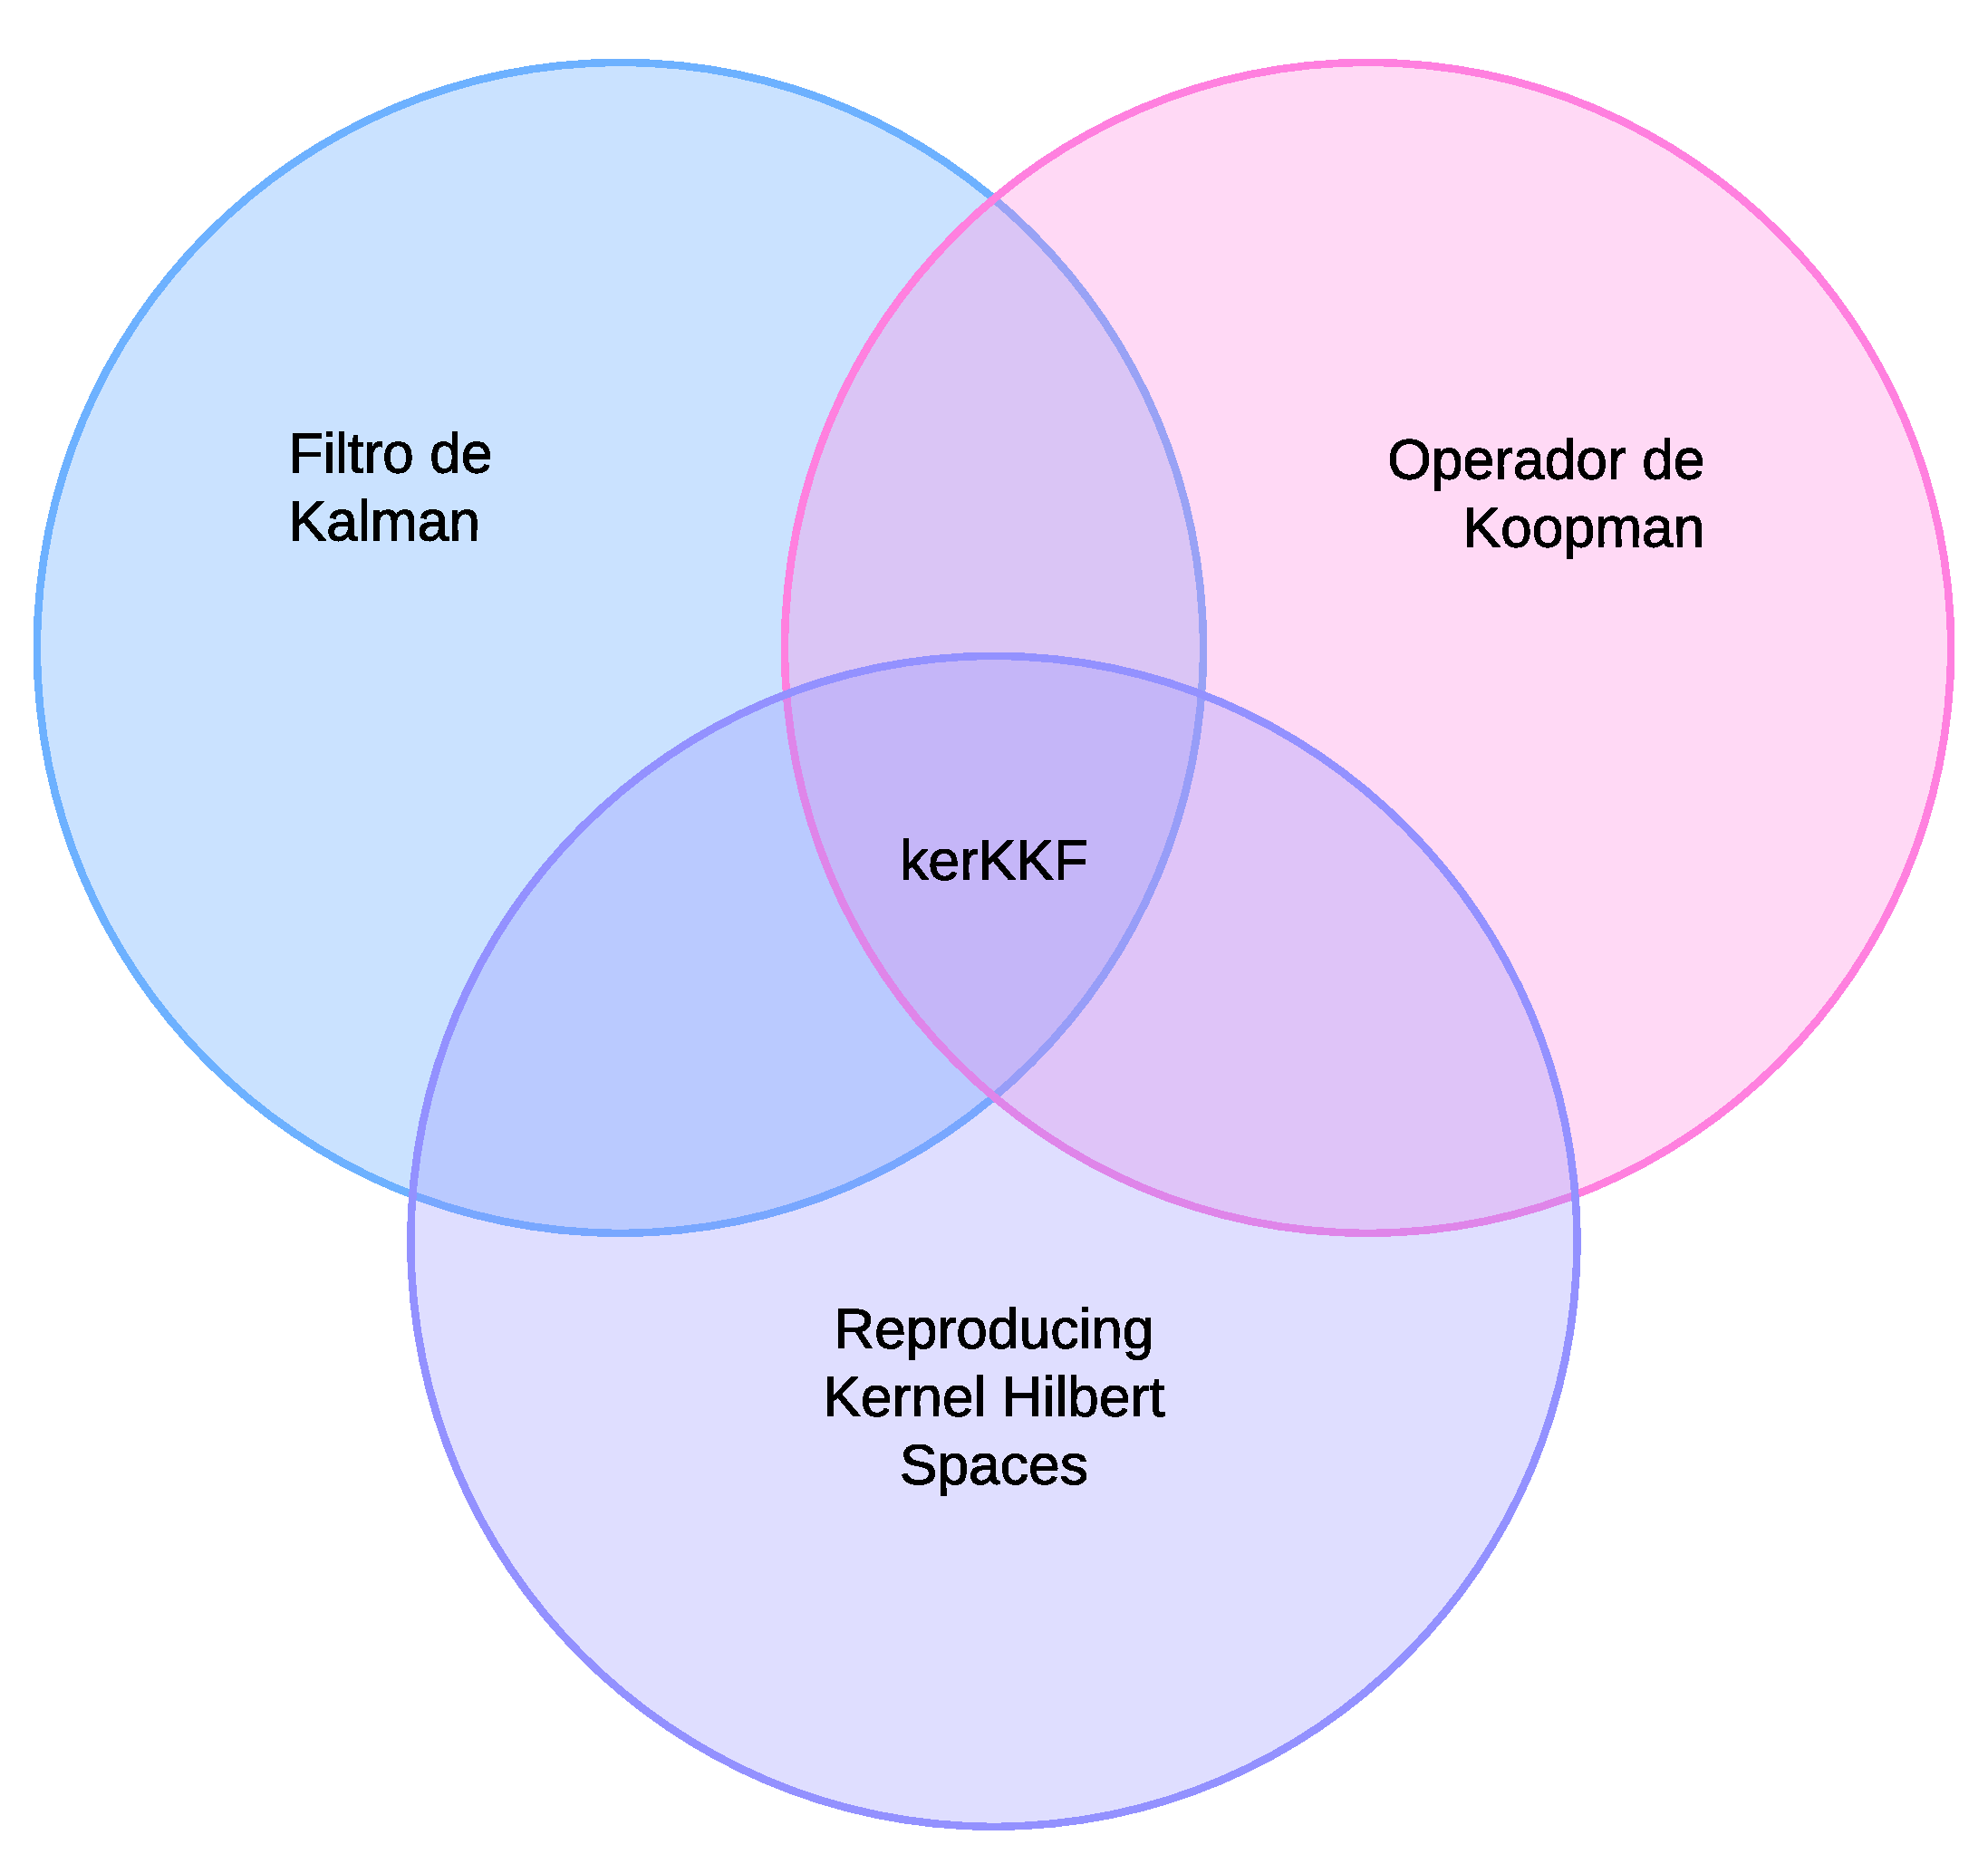
\includegraphics[width=0.9\linewidth]{img/content/chapter1/Venn_Diagram_Thesis.pdf}
        \caption{Diagrama de intersección de áreas como contribución de este trabajo.}
        \label{fig:venn_diagram}
    \end{subfigure}
    \begin{subfigure}[b]{0.45\linewidth}
        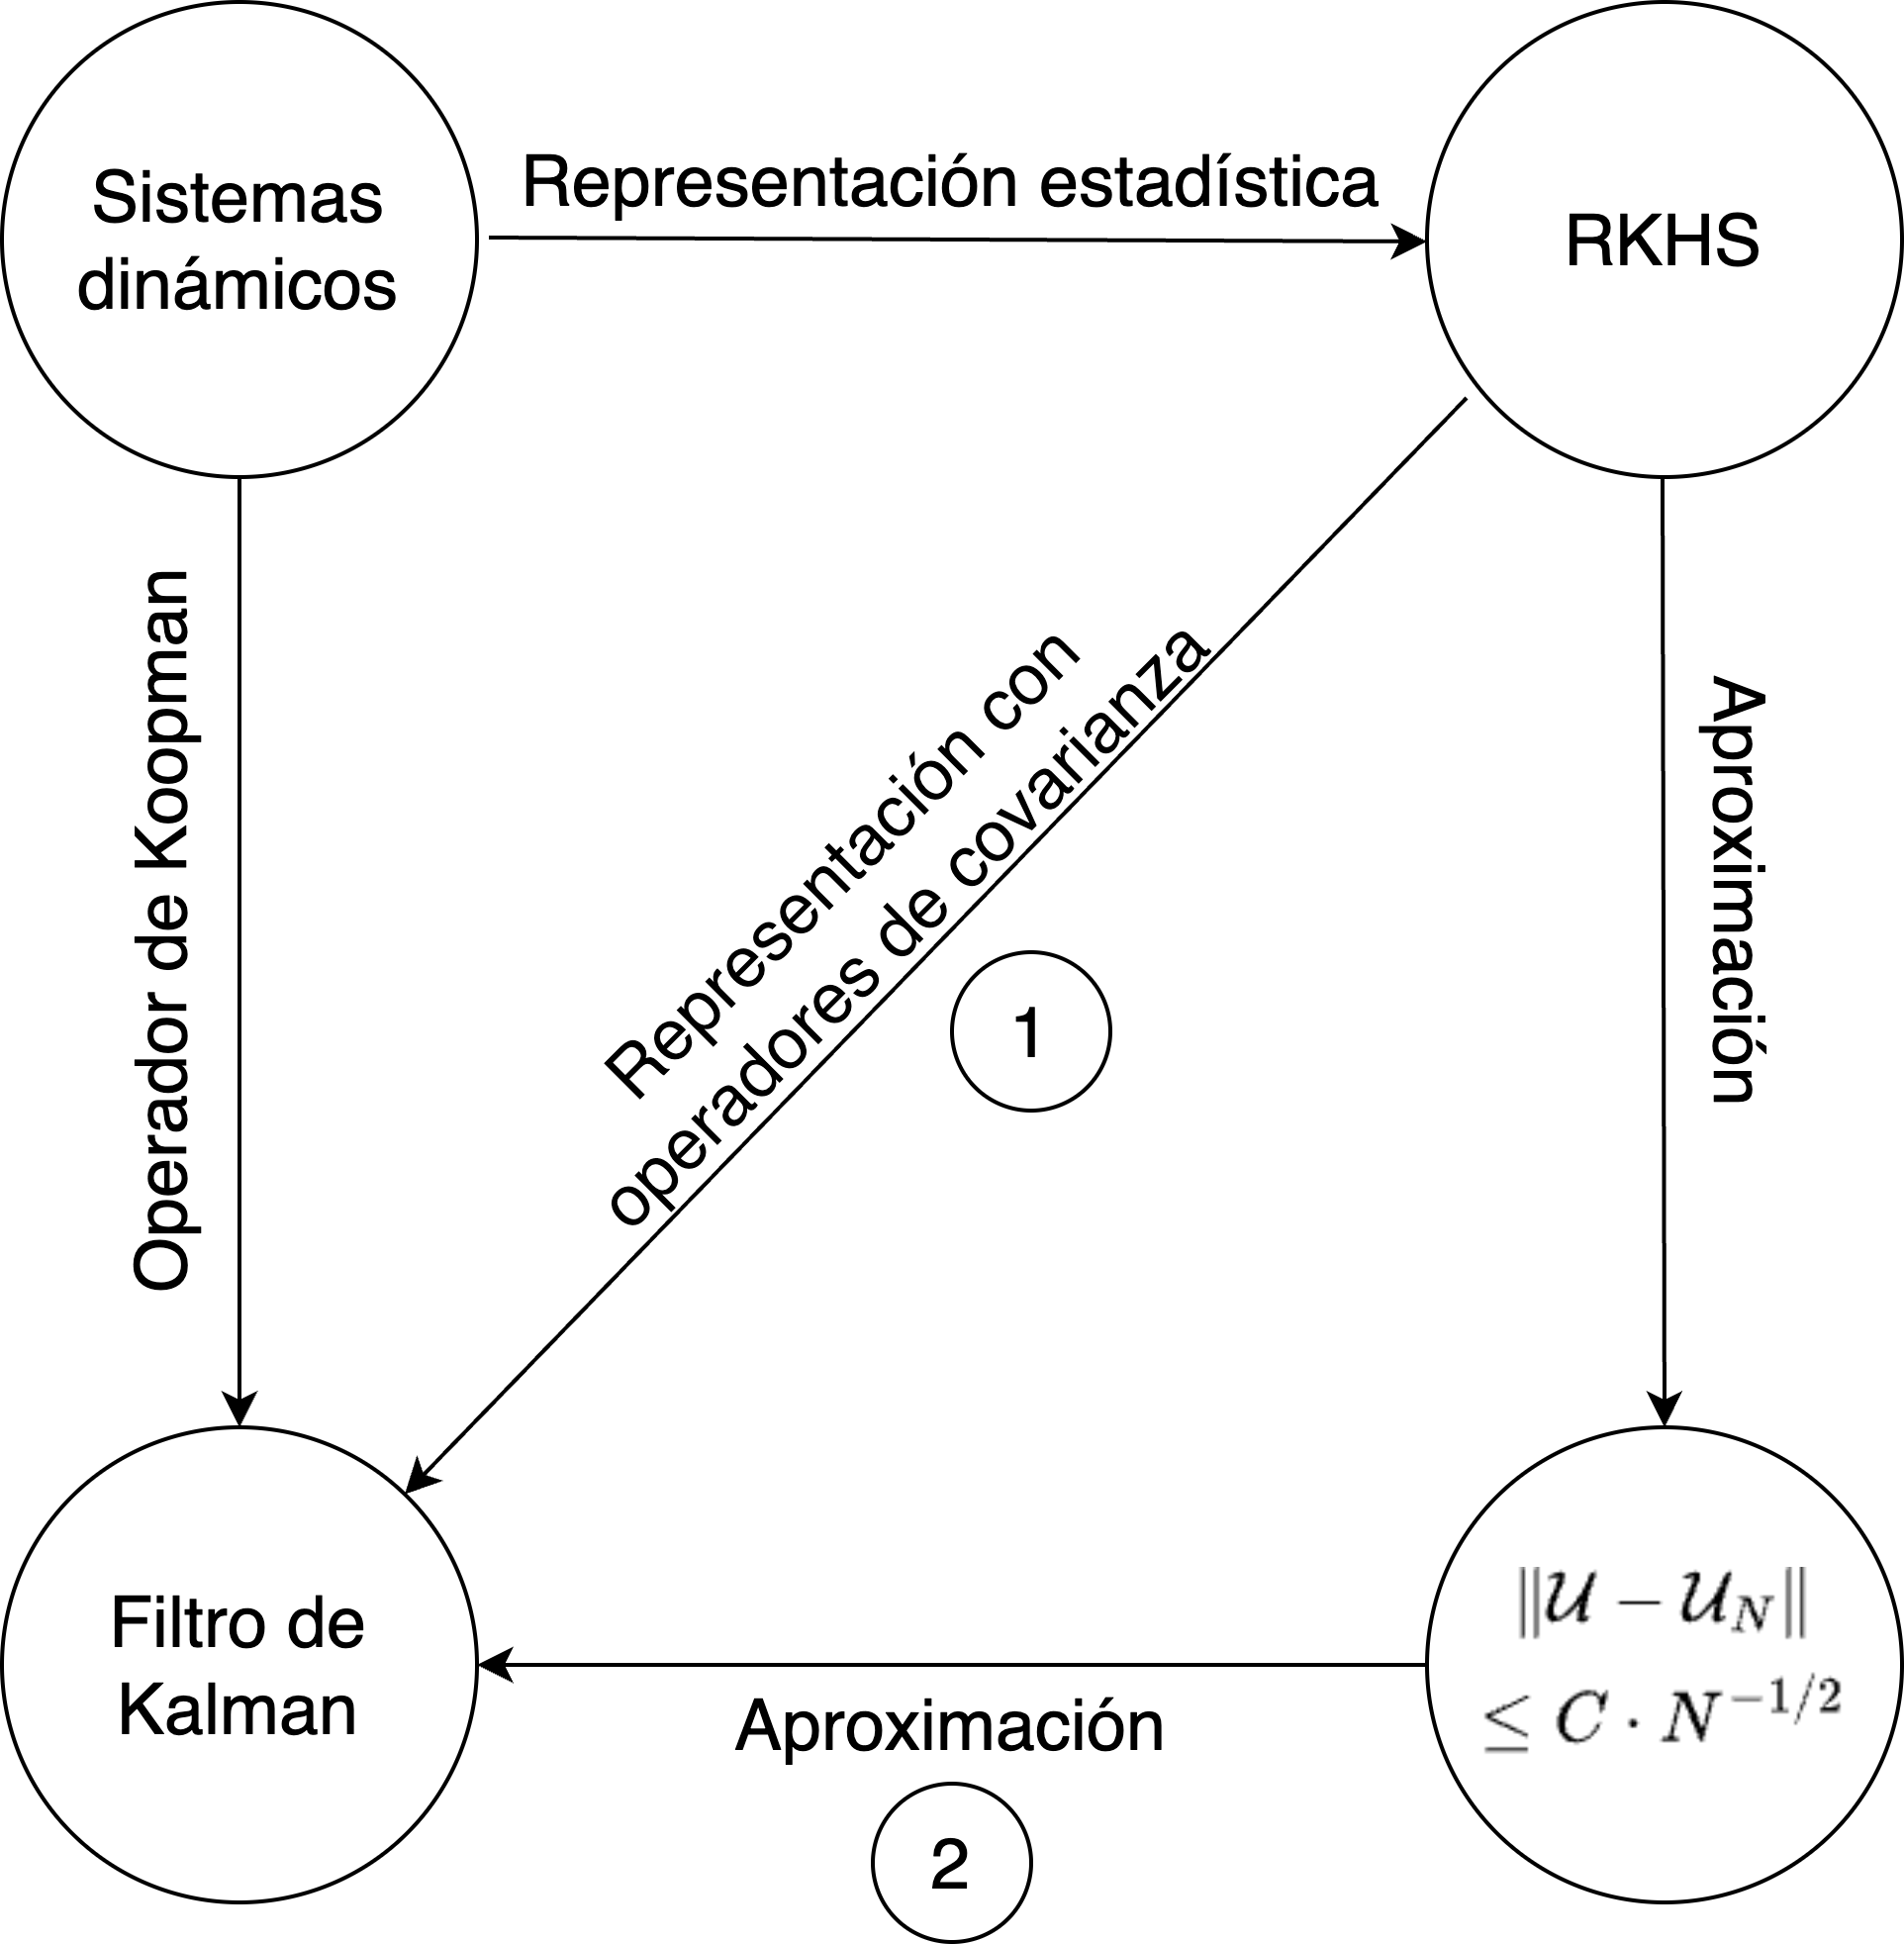
\includegraphics[width=0.9\linewidth]{img/content/chapter1/diag_contri.png}
        \caption{Diagrama de conexiones entre las áreas abordadas en este trabajo.}
        \label{fig:conexiones}
    \end{subfigure}
    \caption{Diagramas explicativos de las contribuciones de esta tesis.}
\end{figure}


% Capítulo 2: Problema resolver, relevancia, algoritmos existentes
% problemática. Estado del arte.
\chapter{Preliminares}
\section{Problema y algoritmos de filtraje}
Se considera un sistema controlado-observado estocástico a tiempo discreto
\begin{align*}
	\mathbf{x}_{k+1} &= \mathbf{f}(t_k, \mathbf{x}_k, \mathbf{u}_k, \mathbf{w}_k) \\
	\mathbf{y}_k &= \mathbf{g}(t_k, \mathbf{x}_k, \mathbf{u}_k, \mathbf{v}_k)
\end{align*}
Donde:
\begin{itemize}
	\item $\mathbf{f}: \R \times \R^{n_x} \times \R^{n_u} \times \R^{n_w} \to \R^{n_x}$ es la función de dinámica.
	\item $\mathbf{g}: \R \times \R^{n_x} \times \R^{n_u} \times \R^{n_v} \to \R^{n_y}$ es la función de observación
\end{itemize}
Siendo $n_x$ la dimensión del estado, $n_y$ la dimensión de la observación, $n_u$ la dimensión del \textit{input}, $n_w$ la dimensión del proceso estocástico en la dinámica y $n_v$ la dimensión del ruido en las observaciones. Se considera una condición inicial $\mathbf{x}_0$, por lo general desconocida sobre la que se coloca un \textit{prior} $X_0$. \\
Se supondrá que tanto $\mathbf{v}_k$ como $\mathbf{w}_k$ son vectores aleatorios centrados tal que $\mathbf{w}_k \indep \mathbf{w}_m, \, \forall k \neq m$, $\mathbf{v}_k \indep \mathbf{v}_m, \, \forall k \neq m$ y $\mathbf{w}_k \indep \mathbf{v}_k, \, \forall k$. Diremos que $\mathbf{w}$ y $\mathbf{v}$ son la perturbación en la dinámica y ruido en la medición, respectivamente. \\
El estudio de sistemas a tiempo continuo, formulados como
\begin{align*}
	\mathbf{x}'(t) &= \mathbf{f}(t, \mathbf{x}(t), \mathbf{u}(t), \mathbf{w}(t)) \\
	\mathbf{y}(t) &= \mathbf{g}(t, \mathbf{x}(t), \mathbf{u}(t), \mathbf{v}(t))
\end{align*}
muchas veces se reduce al caso discreto con esquemas de tipo Euler, por lo que durante esta tesis se mantendrá el foco en sistemas a tiempo discreto, a menos de que se necesite lo contrario. \\
El objetivo en el caso discreto será, en un instante $k$ encontrar un estimador de $\mathbf{x}_{k+\alpha}$, en base a observaciones $\{\Tilde{\mathbf{y}}_k\}_k$, que será denotado por $\hat {\mathbf{x}}_{k+\alpha}$. Dependiendo del valor de $\alpha$ el algoritmo recibirá una categoría diferente:
\begin{itemize}
	\item Predicción: $\alpha > 0$.
	\item Filtraje: $\alpha = 0$.
	\item Suavizado: $\alpha < 0$.
\end{itemize}
Así también se denotará a $\hat {\mathbf{x}}_{k_1|k_2}$ a la estimación del estado en la iteración $k_1$ dadas mediciones hasta la iteración $k_2$, entonces se dirá que $\hat{\mathbf{x}}_{k_1 | k_2}$ es un estado
\begin{itemize}
	\item Suavizado, si $k_2 > k_1$ ($t_2 > t_1$).
	\item Filtrado, si $k_2 = k_1$ ($t_2 = t_1$).
	\item Predicho, si $k_1 > k_2$ ($t_1 > t_2$).
\end{itemize}
El caso del filtraje será el centro durante este trabajo. Un algoritmo de filtraje busca estimar en el tiempo presente el estado en base a observaciones ruidosas, que puede ser entendido como el primer proceso en la estimación del estado de un sistema. \\
Posterior al filtraje de una medición ruidosa, se siguen los procesos de predicción y/o suavizado, siendo el primero la tarea poder estimar estados futuros en base al pasado, sin información del momento a estimar. Mientras que el suavizado es la capacidad de estimar momentos pasados, lo que se utiliza para mejorar las estimaciones presentes.\\
Se denota por $\mathbf{y}_{1:k}$, $\mathbf{u}_{0:k}$ a las observaciones e \textit{inputs}, respectivamente, hasta el tiempo $k \in \N$, a $k \in \N$ le llamaremos el horizonte del problema.  Notar que se considerará que no se tiene una observación de la condición inicial.\\ 
El problema de filtraje se puede formular como un problema de optimización del error cuadrático medio de la estimación, condicional a las observaciones y a los \textit{inputs}
\begin{equation*}
	(P) \quad
	\begin{cases}
		\begin{aligned}
			\text{mín} \quad & \quad \sum_{k=0}^N \E \left [ (\hat{\mathbf{x}}_{k|k} - \mathbf{x}_k)^T(\hat{\mathbf{x}}_{k|k} - \mathbf{x}_k) | \mathbf{y}_{0:k}, \, \mathbf{u}_{0:k}  \right] \\ 
			\text{s.a} \quad & \quad \mathbf{x}_{k+1} = \mathbf{f}(t_k, \mathbf{x}_k, \mathbf{u}_k, \mathbf{w}_k) \\
			\text{} \quad & \quad \mathbf{y}_k = \mathbf{g}(t_k, \mathbf{x}_k, \mathbf{u}_k, \mathbf{v}_k) \\
			\text{} \quad & \quad \mathbf{x}_0 \sim X_0
		\end{aligned}
	\end{cases}
\end{equation*}
Es entonces que el problema $(P)$ tiene como solución al estimador de mínimo error cuadrático. Es sabido de \cite{Kalman1960AProblems, Setoodeh2022NonlinearApplications} que este problema tiene un óptimo global dado por la esperanza condicional, que coincide con la noción de dicho estimador.
\begin{prop}
	El óptimo de $(P)$ viene dado por 
	\begin{equation*}
		\hat{\mathbf{x}}_{k|k} = \E \left [ \mathbf{x}_k | \mathbf{y}_{1:k}, \, \mathbf{u}_{0:k}  \right], \quad \forall k \in \{ 0, \dots, N \}
	\end{equation*}
\end{prop}
\noindent Aunque dicha cantidad no sea computable por métodos clásicos, como Monte Carlo, existen algoritmos para poder calcularla tiempo a tiempo, aunque sea de manera aproximada. 
\subsection{Caso a tiempo discreto, dinámica lineal y ruido centrado}
Para abordar el caso de sistemas dinámicos controlados-observados generales, es importante estudiar primero el caso lineal y con ruidos centrados y segundo momento finito, esto es
\begin{equation}
	\begin{cases}
		\mathbf{x}_{k+1} &= \mathbf{A}_k \mathbf{x}_k + \mathbf{B}_k \mathbf{u}_k + \mathbf{v}_k \\
		\mathbf{y}_k &= \mathbf{C}_k \mathbf{x}_k + \mathbf{D}_k \mathbf{u}_k  + \mathbf{w}_k
	\end{cases}
	\label{eq:lin_disc}
\end{equation}
con $\mathbf{A}_k \in \R^{n_x \times n_x}$, $\mathbf{B}_k \in \R^{n_x \times n_u}$, $\mathbf{C}_k \in \R^{n_y \times n_x}$, $\mathbf{D}_k \in \R^{n_y \times n_u}$,  $\mathbf{v}_k \sim \mathcal{N}(0, \mathbf{Q}_k)$ y $\mathbf{w}_k \sim \mathcal{N}(0, \mathbf{R}_k)$, $\mathbf{Q}_k \in \R^{n_x \times n_x}$, $\mathbf{R}_k \in \R^{n_y \times n_y}$. matrices de covarianzas, se tiene un algoritmo muy utilizado en ingeniería y ciencia, con suficiente fundamentos matemáticos e implementaciones eficientes, denotado el filtro de Kalman en honor a Rudolf E. Kalman, quién propuso el algoritmo por primera vez en \cite{Kalman1960AProblems}. Los detalles del algoritmo se presentan en el pseudo-código del Algoritmo \ref{alg:KF}. \\
\begin{algorithm}
	\caption{Filtro de Kalman}\label{alg:KF}
	\begin{algorithmic}[1]
		\State \textbf{Entrada:} Dinámica discreta como en (\ref{eq:lin_disc}), $\mathbf{x}_0$ \textit{prior} sobre la condición inicial, $\mathbf{y}_{1:N}$ observaciones, $\mathbf{u}_{0:N}$ \textit{inputs}.
		\State \textbf{Salida:} $(\hat{\mathbf{x}}_{k|k})_{k=0}^{N}$ estimador de la trayectoria y $(\hat{\mathbf{P}}_{k|k})_{k=0}^{N}$ matrices de covarianza.
		\State $\hat{\mathbf{x}}_{0|0}   \gets \E [\mathbf{x}_0]$
		\State $\mathbf{P}_{0|0} \gets \E [(\mathbf{x}_0 - \hat{\mathbf{x}}_{0})(\mathbf{x}_0 - \hat{\mathbf{x}}_{0})^T]$
		\For{$k = 0, \dots, N-1$}
		\State $\hat{\mathbf{x}}_{k+1|k} \gets \mathbf{A}_k \mathbf{x}_{k|k} + \mathbf{B}_k \mathbf{u}_k$
		\Comment{Estimación a priori}
		\State $\mathbf{P}_{k+1|k} \gets \mathbf{A}_k \mathbf{P}_{k|k} \mathbf{A}_k^T + \mathbf{Q}_k$
		\Comment{Error de covarianza a priori}
		\State $\hat{\mathbf{y}}_{k+1|k} \gets \mathbf{C}_{k+1} \hat{\mathbf{x}}_{k+1|k}$ 
		\Comment{Estimación de observación a priori}
		\State $\mathbf{e}_{\mathbf{y}_{k+1|k}} \gets \mathbf{y}_{k+1} - \hat{\mathbf{y}}_{k+1|k}$
		\Comment{Error a priori (innovación)}
		\State $\mathbf{K}_{k+1} \gets \mathbf{P}_{k+1|k} \mathbf{C}^T_{k+1} (\mathbf{C}_{k+1} \mathbf{P}_{k|k} \mathbf{C}^T_{k+1}+ \mathbf{R}_{k+1})^{-1}$
		\Comment{Ganancia de Kalman}
		\State $\hat{\mathbf{x}}_{k+1|k+1} \gets \hat{\mathbf{x}}_{k+1|k} + \mathbf{K}_{k+1} \mathbf{e}_{\mathbf{y}_{k+1|k}}$
		\Comment{Error a posteriori}
		\State $\mathbf{P}_{k+1|k+1} \gets (\mathbf{I} - \mathbf{K}_{k+1} \mathbf{C}_{k+1}) \mathbf{P}_{k+1|k}$
		\Comment{Error de covarianza a posteriori}
		\EndFor
	\end{algorithmic}
\end{algorithm}\\
El siguiente resultado le da toda su validez al algoritmo del Filtro de Kalman, que es probado en el artículo original \cite{Kalman1960AProblems}.
\begin{prop}
	El algoritmo del filtro de Kalman devuelve una secuencia $(\hat{\mathbf{x}}_{k|k})_k$ tal que 
	\begin{equation*}
		\hat{\mathbf{x}}_{k|k} = \E \left [ \mathbf{x}_k | \mathbf{y}_{1:k}, \, \mathbf{u}_{0:k}  \right], \quad \forall k \in \{ 0, \dots, N \}
	\end{equation*}
\end{prop}
\noindent Como consecuencia del hecho de que en el contexto Gaussiano el estimador de mínimo error cuadrático medio coincide con el estimador de máximo a posteriori, se tiene el siguiente resultado.
\begin{prop}
	El algoritmo del filtro de Kalman devuelve una secuencia $(\hat{\mathbf{x}}_{k|k})_k$ tal que 
	\begin{equation*}
		\hat{\mathbf{x}}_{k|k} \in \arg \max_{\hat{\mathbf{x}}_{k|k}} p (\hat{\mathbf{x}}_{k|k} | \mathbf{y}_{1:k}, \, \mathbf{u}_{0:k})
	\end{equation*}
\end{prop}

\subsection{Caso a tiempo discreto no lineal general}
A diferencia del caso anterior, en el caso no lineal general hay muchos algoritmos propuestos, siendo los más clásicos las variantes del filtro de Kalman, como el \textit{Extended Kalman Filter} (EKF) y el \textit{Unscented Kalman Filter} (UKF), pero se sabe que resultan ser subóptimos \cite{Setoodeh2022NonlinearApplications}.\\ 
A pesar de que dichos algoritmos reciben dinámicas no lineales, siguen suponiendo que el ruido es aditivo, centrado y Gaussiano. Se verá en secciones posteriores que esto no es un impedimento para poder ejecutarlos, pero una familia de métodos se han construido para el caso más general, cuyos representantes más famosos son los filtros de partículas.\\
Con el motivo de no extender más este informe solo se expondrá el algoritmo de EKF. Para esta sección se supondrá que la dinámica es de la forma
\begin{equation}
	\begin{aligned}
		\mathbf{x}_{k+1} &= \mathbf{f}(t_k, \mathbf{x}_k, \mathbf{u}_k) + \mathbf{w}_k \\
		\mathbf{y}_k &= \mathbf{g}(t_k, \mathbf{x}_k, \mathbf{u}_k) + \mathbf{v}_k 
	\end{aligned}
	\label{eq:no_lin_disc_add}
\end{equation}
Con $\mathbf{w}_k \sim \mathcal{N}(0, \mathbf{Q}_k)$ y $\mathbf{v}_k \sim \mathcal{N}(0, \mathbf{R}_k)$. 
El algoritmo de \textit{Extended Kalman Filter}, cuyo pseudo-código puede visualizarse en el algoritmo \ref{alg:EKF}, busca linearizar el sistema a primer orden vía su Jacobiano, tanto para $\mathbf{f}$ como para $\mathbf{g}$ de manera de generar las matrices $\mathbf{A}_k$ y $\mathbf{C}_k$ necesarias para el Filtro de Kalman, respectivamente. \\
A pesar de los simple que parece la adaptación de este algoritmo al caso no lineal, ilustra que extender el filtro de Kalman al caso no lineal se basa en una linealización de la dinámica, en este caso vía Jacobiano, pero podrían existir otras, que es en lo que se basará el filtro creado durante este trabajo.

\begin{algorithm}
	\caption{\textit{Extended Kalman Filter}}\label{alg:EKF}
	\begin{algorithmic}[1]
		\State \textbf{Entrada:} Dinámica discreta como en (\ref{eq:no_lin_disc_add}), $\mathbf{x}_0$ \textit{prior} sobre la condición inicial,  $\mathbf{y}_{1:N}$ observaciones, $\mathbf{u}_{0:N}$ \textit{inputs}.
		\State \textbf{Salida:} $(\hat{\mathbf{x}}_{k|k})_{k=0}^{N}$ estimador de la trayectoria y $(\hat{\mathbf{P}}_{k|k})_{k=0}^{N}$ matrices de covarianza.
		\State $\hat{\mathbf{x}}_{0|0}   \gets \E [\mathbf{x}_0]$
		\State $\mathbf{P}_0 \gets \E [(\mathbf{x}_0 - \hat{\mathbf{x}}_{0})(\mathbf{x}_0 - \hat{\mathbf{x}}_{0})^T]$
		\For{$k = 0, \dots, N-1$}
		\State $\mathbf{A}_k \gets \nabla _\mathbf{x} \mathbf{f} (t_k, \hat{\mathbf{x}}_{k|k}, \mathbf{u}_k)$
		\Comment{Linealización de la función de dinámica}
		
		\State $\hat{\mathbf{x}}_{k+1|k} \gets \mathbf{f}(t_k, \hat{\mathbf{x}}_{k|k}, \mathbf{u}_k)$
		\Comment{Estimación a priori}
		\State $\mathbf{P}_{k+1|k} \gets \mathbf{A}_k \mathbf{P}_{k|k} \mathbf{A}_k^T + \mathbf{Q}_k$
		\Comment{Error de covarianza a priori}
		\State $\mathbf{C}_{k+1} \gets \nabla_\mathbf{x} \mathbf{g} (t_k, \hat{\mathbf{x}}_{k+1|k}, \mathbf{u}_k)$
		\Comment{Linealización de la función de observación}
		\State $\hat{\mathbf{y}}_{k+1|k} \gets \mathbf{g}(t_k, \hat{\mathbf{x}}_{k+1|k}, \mathbf{x}_{k+1})$ 
		\Comment{Estimación de observación a priori}
		\State $\mathbf{e}_{\mathbf{y}_{k+1|k}} \gets \mathbf{y}_{k+1} - \hat{\mathbf{y}}_{k+1|k}$
		\Comment{Error a priori (innovación)}
		\State $\mathbf{K}_{k+1} \gets \mathbf{P}_{k+1|k} \mathbf{C}^T_{k+1} (\mathbf{C}_{k+1} \mathbf{P}_{k|k} \mathbf{C}^T_{k+1} + \mathbf{R}_{k+1})^{-1}$
		\Comment{Ganancia de Kalman}
		\State $\hat{\mathbf{x}}_{k+1|k+1} \gets \hat{\mathbf{x}}_{k+1|k} + \mathbf{K}_{k+1} \mathbf{e}_{y_{k+1|k}}$
		\Comment{Error a posteriori}
		\State $\mathbf{P}_{k+1|k+1} \gets (\mathbf{I} - \mathbf{K}_{k+1} \mathbf{C}_{k+1}) \mathbf{P}_{k+1|k}$
		\Comment{Error de covarianza a posteriori}
		\EndFor
	\end{algorithmic}
\end{algorithm}

El algoritmo del \textit{Unscented Kalman Filter} (UKF), pseudo-código del algoritmo \ref{alg:UKF}, se basa en generar puntos de muestra (llamados puntos sigma) alrededor de la estimación actual del estado del sistema. Estos puntos permiten representar la distribución estadística de la estimación sin necesidad de calcular derivadas. Al propagar estos puntos sigma a través del modelo no lineal, el UKF logra realizar estimaciones en el siguiente instante de tiempo, capturando de manera precisa las propiedades no lineales del sistema. Esta estrategia hace que el UKF sea una alternativa robusta al \textit{Extended Kalman Filter} (EKF) para el seguimiento y la estimación en sistemas no lineales. Aún así, el algoritmo puede ser costoso en la práctica y es necesaria una gran cantidad de puntos sigma para lograr una estimación fiable.

\begin{algorithm}
	\caption{\textit{Unscented Kalman Filter}}\label{alg:UKF}
	\begin{algorithmic}[1]
		\State \textbf{Entrada:} Dinámica discreta como en (\ref{eq:no_lin_disc_add}), $\mathbf{x}_0$ \textit{prior} sobre la condición inicial,  $\mathbf{y}_{1:N}$ observaciones, $\mathbf{u}_{0:N}$ \textit{inputs}.
		\State \textbf{Salida:} $(\hat{\mathbf{x}}_{k|k})_{k=0}^{N}$ estimador de la trayectoria y $(\hat{\mathbf{P}}_{k|k})_{k=0}^{N}$ matrices de covarianza.
		
		\State \textbf{Inicialización:}
		\State $\hat{\mathbf{x}}_{0|0}   \gets \E [\mathbf{x}_0]$
		\State $\mathbf{P}_0 \gets \E [(\mathbf{x}_0 - \hat{\mathbf{x}}_{0})(\mathbf{x}_0 - \hat{\mathbf{x}}_{0})^T]$
		
		\For{$k = 1, 2, \dots, N$}
		
		\State Calcular los puntos sigma $\chi$ usando la estimación del estado actual $\hat{\mathbf{x}}_{k-1}$ y la covarianza $\mathbf{P}_{k-1}$. Asignar pesos a los puntos sigma de acuerdo con pesos predefinidos $W_m$ (para la media) y $W_c$ (para la covarianza).
		
		\State $\chi_{k|k-1}^{(i)} \gets \mathbf{f}(t_k, \chi_{k-1}^{(i)}, \mathbf{u}_k)$
		\Comment Propagar cada punto sigma a través de la dinámica.
	
		\State $\hat{\mathbf{x}}_{k|k-1} \gets \sum_{i} W_m^{(i)} \chi_{k|k-1}^{(i)}$
		\Comment Calcular la media del estado predicho.
		
		\State Calcular la covarianza predicha:
		\[
		\mathbf{P}_{k|k-1} = \sum_{i} W_c^{(i)} \left( \chi_{k|k-1}^{(i)} - \hat{\mathbf{x}}_{k|k-1} \right) \left( \chi_{k|k-1}^{(i)} - \hat{\mathbf{x}}_{k|k-1} \right)^\top + \mathbf{Q}_k
		\]
		
		\State $\gamma_{k}^{(i)} = \mathbf{h}(t_k, \chi_{k|k-1}^{(i)}, \mathbf{u}_k)$
		\Comment{Pasar cada punto sigma predicho a través de la observación.}
		
		\State $\hat{\mathbf{y}}_k = \sum_{i} W_m^{(i)} \gamma_{k}^{(i)}$
		\Comment{Calcular la media de la medición predicha.}
		\State Calcular la covarianza de la medición:
		\[
		 \mathbf{S}_k = \sum_{i} W_c^{(i)} \left( \gamma_{k}^{(i)} - \hat{ \mathbf{y}}_k \right) \left( \gamma_{k}^{(i)} - \hat{\mathbf{y}}_k \right)^\top + \mathbf{R}_k
		\]
		\State Calcular la covarianza cruzada:
		\[
		\mathbf{C}_k = \sum_{i} W_c^{(i)} \left( \chi_{k|k-1}^{(i)} - \hat{\mathbf{x}}_{k|k-1} \right) \left( \gamma_{k}^{(i)} - \hat{\mathbf{x}}_k \right)^\top
		\]

		\State $\mathbf{K}_k = \mathbf{C}_k \mathbf{S}_k^{-1}$
		\Comment{Calcular la ganancia de Kalman.}
		\State $\hat{ \mathbf{x}}_k = \hat{ \mathbf{x}}_{k|k-1} +  \mathbf{K}_k ( \mathbf{y}_k - \hat{ \mathbf{y}}_k)$ 
		\Comment{Actualizar la estimación del estado.}
		\State $\mathbf{P}_k =  \mathbf{P}_{k|k-1} -  \mathbf{K}_k \mathbf{S}_k  \mathbf{K}_k^\top$
		\Comment{Actualizar la covarianza.}
		
		\EndFor
		
	\end{algorithmic}
\end{algorithm}

Los Filtros de Partículas (PF) o algoritmos de \textit{Sequential Monte Carlo} (SMC) \cite{Kemp2003AnMethods, Wills2023SequentialReview} son una familia de métodos que estiman el estado de sistemas dinámicos no lineales y/o no gaussianos mediante técnicas de muestreo tipo Monte Carlo. Estos algoritmos representan la distribución de probabilidad del estado mediante un conjunto de partículas, que son muestras aleatorias ponderadas según su probabilidad. La precisión de estos filtros depende críticamente del proceso de resampling, un paso fundamental que evita la degeneración de partículas al eliminar aquellas con pesos bajos y duplicar las más probables. Esto permite que los filtros de partículas mantengan una representación precisa de la distribución posterior en cada paso de tiempo, adaptándose dinámicamente a la complejidad del sistema.
Para el algoritmo se considerará que los modelos vienen representados por distribuciones de probabilidad, una de transición para la dinámica  \( p(\mathbf{x}_k | \mathbf{x}_{k-1}) \) y para la observación \( p(\mathbf{y}_k | \mathbf{x}_k) \).

\begin{algorithm}
	\caption{Filtro de Partículas}
	\begin{algorithmic}[1]
		
		\State \textbf{Entrada:} Modelo de dinámica \( p(\mathbf{x}_k | \mathbf{x}_{k-1}) \), modelo de medición \( p(\mathbf{y}_k | \mathbf{x}_k) \), observaciones \( \mathbf{y}_{1:k} \), número de partículas \( N_p \), estado inicial \( \{ \mathbf{x}_0^{(i)} \}_{i=1}^{N_p} \)
		\State \textbf{Salida:} Estimación del estado basada en la distribución ponderada de partículas \( \{ \mathbf{x}_k^{(i)}, w_k^{(i)} \}_{i=1}^{N_p} \)
		
		\For{$i = 1, \dots, N_p$}
		\State Generar la partícula inicial \( \mathbf{x}_0^{(i)} \) de la distribución inicial \( p(\mathbf{x}_0) \)
		\State Asignar el peso inicial \( w_0^{(i)} = \frac{1}{N_p} \)
		\EndFor
		
		\For{$k = 1, 2, \dots, N$}
		
		\For{$i = 1, \dots, N_p$}
		\State Muestrear \( \mathbf{x}_k^{(i)} \sim p(\mathbf{x}_k | \mathbf{x}_{k-1}^{(i)}) \) \Comment{Propagar cada partícula por la dinámica.}
		\EndFor
		
		\For{$i = 1, \dots, N_p$}
		\State \( w_k^{(i)} = w_{k-1}^{(i)} \cdot p(\mathbf{y}_k | \mathbf{x}_k^{(i)}) \) \Comment{Actualizar peso basado en la observación.}
		\EndFor
		
		\State \( w_k^{(i)} = \frac{w_k^{(i)}}{\sum_{j=1}^{N_p} w_k^{(j)}} \)
		\Comment{Normalizar los pesos.}
		
		\If{la degeneración de partículas es alta}
		\State Re-samplear las partículas \( \{ \mathbf{x}_k^{(i)}, w_k^{(i)} \}_{i=1}^{N_p} \) según sus pesos \( w_k^{(i)} \)
		\State Reiniciar pesos: \( w_k^{(i)} = \frac{1}{N_p} \) para todas las partículas
		\EndIf
		
		\EndFor
		
	\end{algorithmic}
\end{algorithm}

Un aspecto importante de los Filtros de Partículas es que su orden de convergencia ha sido demostrado como $O(N_p^{-1/2})$ \cite{Crisan2002APractitioners, Chopin2020AnCarlo}, es decir, la precisión del método aumenta proporcionalmente a la raíz cuadrada inversa del número de partículas utilizadas. Este número de partículas, que se elige como parámetro del filtro, controla directamente el error de estimación. Esta cota de error se tomará como referencia de comparación en el presente trabajo.

% RKHS
\section{Reproducing Kernel Hilbert Spaces}
Esta sección se basa en \cite{Wendland2004ScatteredApproximation} y \cite{Berlinet2004ReproducingStatistics}, aunque una versión más moderna de los resultados se puede encontrar en \cite{Saitoh2016TheoryApplications}. Sea \( \X \) un espacio topológico, y denote \(\C^\X\) al espacio de todas las funciones de \( \X \) en los números complejos. 

\begin{defn}[Reproducing Kernel Hilbert Space (RKHS)]  
Un espacio de Hilbert \( \mathcal{H} \subset \C^\X \) se dice un RKHS si existe una función \( k: \X \times \X \to \C \), llamada \textit{kernel reproduciente}, tal que:
\begin{enumerate}
    \item \( k_p \equiv K(\cdot, p) \in \mathcal{H}, \, \forall p \in E \).
    \item \( f(p) = \langle f, k_p \rangle_{\mathcal{H}}, \quad \forall p \in E, \, \forall f \in \mathcal{H}. \)
\end{enumerate}
\end{defn}

\noindent La segunda propiedad, conocida como \textit{propiedad reproduciente}, es fundamental en la teoría de los RKHS y da paso a muchas de las propiedades relevantes en estos espacios, como aquellas que se presentarán a continuación. Denotamos por \( \mathcal{H}_K(E) \) al espacio de Hilbert de funciones de \( E \) en \( \C \) cuyo kernel reproduciente es \( k \).

El siguiente lema proporciona una condición necesaria y suficiente para que un espacio de Hilbert dado posea un kernel reproduciente.

\begin{lema}
Un espacio de Hilbert \( \mathcal{H} \subset \C^\X \) posee un kernel reproduciente si y solo si los funcionales de evaluación \( e_p: \mathcal{H} \to \C \), definidos por \( e_p(f) = f(p) \), son continuos en \( \mathcal{H} \).
\end{lema}

\noindent Para construir un RKHS sobre un espacio topológico \( \X \), se introduce la siguiente definición.

\begin{defn}[Función semi-definida positiva]  
Una función \( k: \X \times \X \to \C \) se dice semi-definida positiva si para todo \( n \geq 1 \), \( (c_1, \dots, c_n) \in \C^n \), y \( (x_1, \dots, x_n) \in \X^n \), se cumple que:
\[
\sum_{i=1}^n \sum_{j=1}^n c_i \bar{c_j} K(x_i, x_j) \geq 0.
\]
\end{defn}

\noindent Esta propiedad es equivalente a que, para cada \( n \in \N \) y toda colección \( (x_1, \dots, x_n) \in \X^n \), la matriz  
\[
G = \left( k(x_i, x_j) \right)_{1 \leq i, j \leq n}
\]
sea Hermitiana y semi-definida positiva. Dicha matriz se denomina matriz Grammiana del kernel asociada a \( \{ x_i \}_{i=1}^n \), o simplemente matriz Grammiana cuando no haya lugar a confusión.

Finalmente, el siguiente lema describe cómo construir una función semi-definida positiva a partir de un espacio de Hilbert dado.

\begin{lema}
Sea \( \mathcal{H} \subset \C^\X \) un espacio de Hilbert con producto interno \( \langle \cdot, \cdot \rangle_\mathcal{H} \), y sea \( \varphi : \X \to \mathcal{H} \). Entonces, la función \( k: \X \times \X \to \C \), definida como
\[
k(x,y) = \langle \varphi(x), \varphi(y) \rangle_\mathcal{H},
\]
es semi-definida positiva.
\end{lema}

\noindent A continuación, dado un kernel \( k \) semi-definido positivo, se presentan un lema y un teorema que describen el comportamiento de un RKHS.

\begin{lema}
Sea \( \mathcal{H}_0 \) un subespacio de \( \C^\X \) en el cual se define un producto interno \( \langle \cdot, \cdot \rangle_{\mathcal{H}_0} \), con norma asociada \( \|\cdot\|_{\mathcal{H}_0} \). Entonces, para que exista un espacio de Hilbert \( \mathcal{H} \) tal que:
\begin{enumerate}
    \item[(1)] \( \mathcal{H}_0 \subset \mathcal{H} \subset \C^\X \), y la topología definida en \( \mathcal{H}_0 \) por el producto interno \( \langle \cdot, \cdot \rangle_{\mathcal{H}_0} \) coincida con la topología inducida en \( \mathcal{H}_0 \) por \( \mathcal{H} \),
    \item[(2)] \( \mathcal{H} \) posea un kernel reproduciente \( k \),
\end{enumerate}
es necesario y suficiente que:
\begin{enumerate}
    \item[(i)] Los funcionales de evaluación \( (e_t)_{t \in \X} \) sean continuos en \( \mathcal{H}_0 \),
    \item[(ii)] Cualquier sucesión de Cauchy \( (f_n) \) en \( \mathcal{H}_0 \) que converge puntualmente a cero, también converge a cero en el sentido de la norma.
\end{enumerate}
\end{lema}

\begin{teo}[Moore–Aronszajn \cite{Aronszajn1950TheoryKernels}]
Sea \( k \) una función semi-definida positiva en \( \X \times \X \). Entonces, existe un único espacio de Hilbert \( \mathcal{H} \subset \C^\X \) con \( k \) como kernel reproduciente. El subespacio \( \mathcal{H}_0 \) de \( \mathcal{H} \), generado por las funciones \( (k(\cdot, x))_{x \in \X} \), es denso en \( \mathcal{H} \), y \( \mathcal{H} \) coincide con el conjunto de funciones en \( \X \) que son límites puntuales de sucesiones de Cauchy en \( \mathcal{H}_0 \), con el producto interno definido por
\[
\langle f, g \rangle_{\mathcal{H}_0} = \sum_{i=1}^n \sum_{j=1}^m \alpha_i \bar{\beta}_j k(y_j, x_i),
\]
donde
\[
f(\cdot) = \sum_{i=1}^n \alpha_i k(\cdot, x_i), \quad g(\cdot) = \sum_{j=1}^m \beta_j k(\cdot, y_j),
\]
para \( (x_1, \dots, x_n) \in E^n \) y \( (y_1, \dots, y_m) \in \X^m \).
\end{teo}

\noindent El siguiente teorema permite transferir las propiedades de un RKHS a un espacio \( \ell^2 \), el cual resulta, en general, más sencillo de manipular.

\begin{teo}
Una función \( K: \X \times \X \to \C \) es un kernel reproduciente si y solo si existe una función \( \varphi: E \to \ell^2 (\Tilde{\X}) \), para algún espacio \( \ell^2(\Tilde{\X}) \), tal que para todo \( (x, y) \in \X \times \X \),
\[
k(x, y)= \langle \varphi(x), \varphi(y) \rangle_{\ell^2(\Tilde{\X})}.
\]
Además, el espacio \( \ell^2(\Tilde{\X}) \) es isométrico a \( \H_k(\X) \) a través de una isometría \( T: \X \to \ell^2(\Tilde{\X}) \), y la función \( \varphi \) viene dada por \( \varphi(x) = T(k(\cdot, x)) \). Dicha función \( \varphi \) se denomina el \textit{feature map} asociado a \( k \).
\end{teo}
En la literatura existen muchos kernels que son de utilidad en uno u otro contexto. A efectos de este trabajo se considerará el kernel de Matérn que, como se expondrá a lo largo de este escrito, posee muy buenas propiedades.
\begin{defn}
Se define el kernel de Matérn con parámetro de suavización \( \nu > 0 \) y ancho de banda \( \gamma > 0 \) como:
\[
k_{\nu}(x,y) = \frac{2^{1-\nu}}{\Gamma(\nu)} \left( \sqrt{2\nu} \frac{\|x-y\|}{\gamma} \right)^\nu B_\nu \left( \sqrt{2\nu} \frac{\|x-y\|}{\gamma} \right),
\]
donde \( \Gamma \) es la función Gamma y \( B_\nu \) es la función modificada de Bessel de segundo tipo de parámetro \( \nu \).

\end{defn}

El kernel de Matérn tiene una estrecha relación con los espacios de Sobolev fraccionarios, por lo que se introducen conceptos claves, como la definición de dicho espacio en $\R^d$ y la condición de cono interior.

\begin{defn}[Espacio de Sobolev fraccionario \cite{Adams2003SobolevSpaces}] Se define el espacio de Sobolev de regularidad $s > 0$ como
\[
H^s(\mathbb{R}^n) = \left\{ f \in L^2(\mathbb{R}^n) : \widehat{f}(\cdot)(1 + \|\cdot\|_2^2)^{s/2} \in L^2(\mathbb{R}^n) \right\},
\]
donde \( \widehat{f} \) denota la transformada de Fourier de \( f \).
\label{def:frac_sob}
\end{defn}

\begin{defn}[Condición de cono interior \cite{Wendland2004ScatteredApproximation}]
Un conjunto \( \Omega \subset \mathbb{R}^n \) satisface la condición del cono interior si existe un ángulo \( \theta \in (0, \pi/2) \) y un radio \( r > 0 \) tales que, para cada \( x \in \Omega \), existe \( \xi(x) \in \mathbb{R}^n \), con \( \|\xi(x)\|_2 = 1 \), de modo que el cono
\[
C(x, \xi(x), \theta, r) := \{x + \lambda y : y \in \mathbb{R}^n, \|y\| = 1, y^\top \xi(x) \geq \cos \theta, \lambda \in [0, r]\}
\]
está contenido en \( \Omega \).
\end{defn}
El siguiente teorema entrega una condición clave para los desarrollos de este trabajo, que es el hecho de que el kernel de Matérn es equivalente en norma a un espacio de Sobolev.
\begin{teo}[\cite{Wendland2004ScatteredApproximation, Tuo2016AProperties}]
Si \( \mathcal{X} \) es un conjunto compacto que satisface la condición del cono interior y \( k \) es el kernel de Matérn con parámetro \( \nu > 0 \), entonces para \( s = \nu + n/2 \) se cumple que \( \mathcal{H}_k (\mathcal{X}) \) es equivalente en norma a \( H^s (\mathcal{X}) \).
\end{teo}

\begin{obs}
    Si \( \nu = 1/2 \), se tiene que
\[
B_{1/2} (z) = \sqrt{ \frac{\pi}{2} } \frac{e^{-z}}{\sqrt{z}},
\]
por lo que se deduce que:
\[
\begin{aligned}
k (x,y) &= \frac{\sqrt{2}}{\Gamma(1/2)} \left(  \frac{\|x-y\|}{\gamma} \right)^{1/2} \sqrt{ \frac{\pi}{2} } \exp \left( -\frac{\|x-y\|}{\gamma} \right) \left(  \frac{\|x-y\|}{\gamma} \right)^{-1/2} = \exp \left( -\frac{\|x-y\|}{\gamma} \right).
\end{aligned}
\]
En consecuencia, el kernel de Matérn generaliza al kernel Laplace, y el RKHS asociado al kernel Laplace es \( H^{(n+1)/2} \).
\end{obs}
Notar que la definición \ref{def:frac_sob} no es válida cuando se tiene un subconjunto de $\R^n$, pero la deducción de esta propiedad en \cite{Wendland2004ScatteredApproximation} pasa por extender las funciones a todo $\R^n$ y luego aplicar la definición. \\
En las secciones posteriores será de interés hacer un \textit{embedding} de una distribución en un RKHS, para lo que es necesario definir el elemento medio en un RKHS y los operadores de covarianza. Las definiciones y proposiciones que siguen han sido expuestas en \cite{Fukumizu2004DimensionalitySpaces, Song2009HilbertSystems, Muandet2017KernelBeyond}. \\
Sean $\X \subset \R^n$, $\Y \subset \R^p$,  Sea $\mu$ una medida de probabilidad sobre $\X$, $\H$ un RKHS sobre $\X$ con kernel reproduciente $k$ y feature map $\Phi$ y $X$ una variable aleatoria con soporte en $\X$ y $Y$ una variable aleatoria con soporte en $\Y$.
\begin{defn}[Elemento medio \cite{Song2009HilbertSystems}]
	Se define el elemento medio en el RKHS $\H$ como
	
	\begin{equation*}
		\hat \mu = \int_\X \Phi (x) d \mu (x) \in \H
	\end{equation*}
\end{defn}
Se define el producto Kronecker en el contexto de RKHS como un operador multiplicativo y que generaliza el producto Kronecker de vectores.
\begin{defn}[Producto de Kronecker]
    El producto Kronecker en un RKHS se define como
    el siguiente operador de rango 1 para $x, y \in \X$ fijos
	$$ \Phi_\X (x) \otimes \Phi_\X(y) : \H_\X \to \H_\X$$
	\begin{equation*}
		[\Phi_\X (x) \otimes \Phi_\X(y)] \psi = \langle \psi, \Phi_\X (y) \rangle \Phi_\X (x) = \psi (y) \Phi_\X (x)
	\end{equation*}
    \label{def:kronecker}
\end{defn}
Notar que en la última igualdad se utilizó la propiedad reproduciente. Esto motiva la definición del operador de covarianza.
\begin{defn}[Operador de covarianza]
    El operador de covarianza asociado al \textit{feature map} $\Phi$ como $C_X : \H_\X \to \H_\X$ 
    \begin{equation*}
        C_X = \int_\X \Phi_\X (x) \otimes \Phi_\X (x) d \mu_\X (x)
    \end{equation*}
\end{defn}
La definición del operador de covarianza cruzada entre dos variables aleatorias será fundamental en el desarrollo posterior como embedding de las variables en un espacio de Hilbert.
\begin{defn}[Operador de covarianza cruzada]
    El operador de covarianza cruzada asociado a las variables aleatorias $X$ e $Y$ se define como el operador $C_{XY}: \H_\X \to \H_\Y$	
    \begin{equation*}
        C_{X Y} = \E [\Phi_\X (X) \otimes \Phi_\Y (Y)] = \int_\X \int_\Y \Phi_\X (x) \otimes \Phi_\Y (y) \rho_g (x, dy) d \mu_\X (x)
    \end{equation*}
\end{defn}

	El adjunto de estos operadores es sencillo de calcular
	\begin{prop}
		Sea $x \in \X$ e $y \in \Y$, luego
		
		\begin{equation*}
			\left ( \Phi_\X (x) \otimes \Phi_\Y (y) \right )^* = \Phi_\Y (y) \otimes \Phi_\X (x)
		\end{equation*}
	\end{prop}
	\begin{proof}
		Sean $h_\X \in \H_\X$, $h_\Y \in \H_\Y$, luego
		\begin{equation*}
			\langle (\Phi_\X (x) \otimes \Phi_\Y (y)) h_\Y, h_\X \rangle = \langle h_\Y (y) \Phi_\X (x), h_\X \rangle = h_\Y (y) \langle \Phi_\X (x), h_\X \rangle
		\end{equation*}
		Por propiedad reproduciente
		\begin{equation*}
			h_\Y (y) \langle  \Phi_\X (x), h_\X \rangle = h_\Y (y) h_\X (x)
		\end{equation*}
		A la vez
		\begin{equation*}
			\langle h_\Y, (\Phi_\Y (y) \otimes \Phi_\X (x)) h_\X \rangle = \langle h_\Y, h_\X (x) \Phi_\Y (y) \rangle = h_\X (x) 
			\langle h_\Y, \Phi_\Y (y) \rangle =
		\end{equation*}
		Nuevamente, por propiedad reproduciente
		\begin{equation*}
			h_\X (x) 
			\langle h_\Y, \Phi_\Y (y) \rangle =h_\X (x) h_\Y (y) 
		\end{equation*}
		Y se concluye lo pedido.
	\end{proof}
	
	\begin{cor} $(C_{X})^* = C_X$.
	\end{cor}
	Dado que la integral es lineal
	\begin{equation*}
		(C_X)^* = \int_\X (\Phi_\X (x) \otimes \Phi_\X (x))^* d \mu_\X (x) = \int_\X \Phi_\X (x) \otimes \Phi_\X (x) d \mu_\X (x) = C_X
	\end{equation*}
	\begin{cor}
		\begin{equation*}
			(C_{XX^+})^* = C_{X^+X}, \quad (C_{XY})^* = C_{YX}
		\end{equation*}
	\end{cor}
	Esto es directo ya que el operador adjunto y la esperanza son lineales:
	\begin{equation*}
		(C_{X X^+})^* = \E [(\Phi_\X (X) \otimes \Phi_\X (X^+))^*] = \E [\Phi_\X (X^+) \otimes \Phi_\X (X)] = C_{X^+X} 
	\end{equation*}
	\begin{equation*}
		(C_{X Y})^* = \E [(\Phi_\X (X) \otimes \Phi_\Y (Y))^*] = \E [\Phi_\X (Y) \otimes \Phi_\X (X)] = C_{YX} 
	\end{equation*}
La herramienta clave para poder trabajar con el embedding de la esperanza condicional en un espacio de Hilbert será el operador de embedding condicional, cuya correcta definición se revisará en una proposición posterior.
\begin{defn}[Operador de embedding condicional]
    El operador de embedding condicional entre 2 distribuciones $X$ e $Y$, en $\X$ e $\Y$, respectivamente, como el operador $C_{X|Y} : \H_\X \to \H_\Y$ que satisface
    \begin{enumerate}
        \item $\mu_{Y|x} = \mathbb{E}_{Y|X}[\Phi_\Y (Y)|X=x] = C_{Y|X}\Phi_\X (x)$.
        \item $\mathbb{E}_{Y|X}[h(Y)|X=x] = \langle h, \mu_{Y|x} \rangle$.
    \end{enumerate}
\end{defn}
El siguiente teorema indica la existencia y forma del operador de embedding condicional \cite{Fukumizu2004DimensionalitySpaces, Song2009HilbertSystems}.
\begin{teo}
    Suponiendo que \( \mathbb{E}[h(Y)|X = \cdot] \in \mathcal{H}_X \) para cualquier \( h \in \mathcal{H}_Y \) entonces se tiene que
    \[ C_{Y|X} = C_{YX} C_{X}^{-1}.\]
\end{teo}

% Operador de Koopman
\section{Operador de Koopman}
El estudio de sistemas dinámicos, tanto a tiempo continuo como a tiempo discreto, ha sido un amplio campo de estudio en diferentes áreas de la matemática, ciencia e ingeniería. En el presente escrito se aboradará su estudio, tanto teórico como computacional, con el operador de Koopman. \\ Desde un punto de vista más matemático, un trabajo pionero fue el de Koopman en 1931 \cite{Koopman1931HamiltonianSpace} en donde se define el operador de Koopman para sistemas dinámicos con espectro discreto. Lo desarrollado por Koopman fue posteriormente generalizado por Koopman y von Neumann en 1932 \cite{Koopman1932DynamicalSpectra}.\\
En los tiempos recientes, el operador de Koopman ha vuelto a surgir en la literatura para el estudio de sistemas dinámicos no lineales, motivado principalmente por los trabajos de Mezić y Budišić junto a otros colaboradores \cite{Budisic2009AnObservables, Budisic2012GeometryFlows, Budisic2012AppliedKoopmanism}. \\
Aprovechando la linealidad del operador de Koopman, aunque sea a costa de trabajar ahora en dimensión finita, es que se han propuesto técnicas para aproximar el operador vía matrices y así volver muchos problemas no lineales en tareas accesibles en un computador, en donde destacan los trabajos de Schmid \cite{Schmid2008DynamicData} en la creación del DMD y de Williams \cite{Williams2015ADecomposition} en la del EDMD.\\
Posterior a ello, trabajos más modernos se han movido a ver extensiones a otros tipos de sistemas, como sistemas con retardo o sistemas de ecuaciones en derivadas parciales, en donde no solo los trabajos de Mezić han seguido siendo relevantes \cite{Mezic2013AnalysisOperator, Mezic2020SpectrumGeometry, Mezic2022OnOperator}, sino que también los trabajos de Brunton y Kutz han marcado la pauta en ámbitos aún más aplicados \cite{Kaiser2021Data-drivenControl, Brunton2016KoopmanControl, Proctor2018GeneralizingControl, Lusch2018DeepDynamics, Kamb2020Time-delayApplications, NathanKutz2018AppliedSystems}, en donde incluso destacan ya implementaciones a nivel librería de los avances numéricos en la aproximación de Koopman \cite{Pan2024PyKoopman:Operator}.\\
Para introducir la idea y concepto del operador de Koopman a utilizar en este trabajo, se considera primero un sistema dinámico autónomo determinista.
\begin{equation}
	\mathbf{x}_{k+1} = \mathbf{f}(\mathbf{x}_k), \quad k \geq 0
	\label{eq:NL}
	\tag{NL}
\end{equation}
Con $\X \subset \R^n$ el espacio de estados. En este contexto, a las funciones $\varphi: \X \to \C$ se les denotará por \textit{observables} en $\mathcal{F}$ un espacio de Banach, con norma $||\cdot||_\mathcal{F}$. Con esto se puede definir el operador de Koopman asociado a una dinámica en tiempo discreto.
\begin{defn}[Operador de Koopman, tiempo discreto]
    El operador de Koopman asociado a $\mathbf{f}: \X \to \X$ es el operador $\U_\mathbf{f}: \mathcal{F} \to \mathcal{F}$ que se define mediante composición
    \begin{equation*}
	\U_\mathbf{f} \varphi = \varphi \circ \mathbf{f}, \quad \forall \varphi \in \mathcal{F}
    \end{equation*}
\end{defn}
\noindent El operador de Koopman da un panorama global sobre el sistema estudiado y además resulta ser un operador lineal, aunque infinito-dimensional. 
En lo que sigue se omitirá el subíndice $\mathbf{f}$ y se denotará simplemente por $\U$ y $||\U||$ será su norma de operador definida como
$$ ||\U|| = \sup \{ ||\U g||_\mathcal{F} \, : \, ||g||_\mathcal{F} = 1 \} $$
que depende del espacio $\mathcal{F}$ en donde se esté trabajando, aunque en cierto tipos de espacios se cumple lo siguiente.
\begin{prop}
	Para todo espacio de Banach $\mathcal{F}$ que contenga a las funciones constantes, se cumple que $||\U|| \geq 1$.
\end{prop}
Lo deseable para muchas aplicaciones es la continuidad del operador, incluso en muchos espacios se cumple que el operador tenga norma igual a $1$.
\begin{prop}
	Si $\mathcal{F} = L^\infty$, entonces el operador de Koopman es un operador con norma unitaria.
\end{prop}
Un caso aún más interesante, pero difícil de cumplir para un sistema dinámico cualquiera y complicado de comprobar en la práctica, es el caso de un sistema que preserve medida.
\begin{defn}[Sistema dinámico que preserva medida] Sea $\X$ un conjunto, $\mathcal{B}$ una $\sigma$-álgebra sobre $\X$, $\mu : \mathcal{B} \to [0, 1]$ una medida de probabilidad y  $F: \X \to \X$ una función medible. Se dice que $(\X, \mathcal{B}, \mu, \mathbf{f})$ preserva medida si $\mu(A) = \mu(\mathbf{f}^{-1}(A))$.
	
\end{defn}
\begin{prop}
	Sea $\mathcal{B}$ una $\sigma$-álgebra sobre $X$ y $(X, \mathcal{B}, \mu, \mathbf{f})$ un sistema dinámico que preserva medida, entonces si $\mathcal{F} = L^2 (\mu)$, se tiene que $||\U|| = 1$. Es más, $\mathcal{U}$ resulta ser un isomorfismo isométrico, esto es
	$$ \langle g, g \rangle = \langle \mathcal{U}g, \mathcal{U}g \rangle, \, \forall g \in \mathcal{F} $$
\end{prop}
Una motivación inicial para el estudio del operador de Koopman era poder analizar propiedades más explicativas de los sistemás dinámicos, como sus propiedades espectrales.
\begin{defn}[Valores y funciones propias]
	Una función propia del operador de Koopman asociado a la función $\mathbf{f}$ es una función $\phi_\lambda \in \mathcal{F} \setminus \{ 0 \}$ tal que 
	\begin{equation*}
		\U \phi_\lambda = \phi_\lambda \circ \mathbf{f} = \lambda \phi_\lambda
	\end{equation*}
	Con $\lambda \in \C$ su valor propio asociado.
\end{defn}
% \begin{prop}
% 	Para todo valor propio $\mu \in \C$ de $\U$, se tiene que $|\mu| \leq ||\U||$.
% \end{prop}
% \begin{proof}
	%     Sea $\mu \in \C$ valor propio de $\U$ y $\phi_\mu \in \mathcal{F} \setminus \{ 0 \}$ su función propia asociada, entonces
	%     $$||\mu \phi_\mu ||_\mathcal{F} = |\mu| ||\phi_\mu||_\mathcal{F} = ||\U \phi_\mu||_\mathcal{F} \leq ||\U|| \cdot ||\phi_\mu||_\mathcal{F} \leq  ||\phi_\mu||_\mathcal{F} $$
	%     Con lo que se obtiene $|\mu| \leq ||\U||$.
	% \end{proof}
Serán de interés las funciones propias y valores propios del operador de Koopman en el caso en que la dinámica del sistema sea lineal, en donde estas se corresponden con vectores y valores propios de la matriz que caracteriza el sistema.
\begin{prop}
	Si $\mathbf{f}(\mathbf{x}) = \mathbf{A}\mathbf{x}$, con $\mathbf{A} \in \R^{n \times n}$, $\mathcal{F} = C(\R^n; \C)$ y $\mathbf{A}$ posee valores propios $\{\mu_j\}_{j=1}^n$ y vectores propios por izquierda $\{ \mathbf{w}_j \}_{j=1}^n$, es decir $\mathbf{w}_j^T \mathbf{A} = \mu_j \mathbf{w}_j^T$, entonces $\{\mu_j\}_{j=1}^n$ son valores propios de $\U$ con funciones propias asociadas $\phi_j (\mathbf{x}) = \mathbf{w}_j^T \mathbf{x}$.
\end{prop}
% \begin{proof}
	%     Basta verificar que 
	%     \begin{equation*}
		%         \U \phi_j (x) = \phi_j (F(x)) = \phi_j (Ax) = w_j^T A x = \mu_j w_j^T x = \mu_j \phi_j (x)
		%     \end{equation*}
	% \end{proof}
%https://arxiv.org/pdf/1611.01209.pdf
En el contexto lineal, los valores propios $\{\mu_j\}_{j=1}^n$ y $\{ \phi_j\}_{j=1}^n$ se dicen valores y funciones propias principales, respectivamente. \\
Otra propiedad espectral importante es que el producto de funciones propias es función propia, en el caso en que esto haga sentido.
\begin{prop}
	Si $\mathcal{F}$ es cerrado para la multiplicación y $\phi_{\mu_1}, \, \phi_{\mu_2}$ son funciones propias de $\U$ con valores propios asociados $\mu_1$, $\mu_2$, respectivamente, entonces $\phi_{\mu_1} \phi_{\mu_2}$ es función propia de $\U$ con valor propio asociado $\mu_1 \mu_2$.
\end{prop}
% \begin{proof}
	%     Basta verificar que 
	%     \begin{equation*}
		%         \U(\phi_{\mu_1} \phi_{\mu_2})(x) = (\phi_{\mu_1} \phi_{\mu_2} ) (f(x)) = \phi_{\mu_1} (f(x))\phi_{\mu_2} (f(x)) = \mu_1 \phi_{\mu_1} \mu_2 \phi_{\mu_2}
		%     \end{equation*}
	%     Y notar que dado que $|\mu_1|$, $|\mu_2| \leq 1$, entonces $|\mu_1 \mu_2| \leq 1$.
	% \end{proof}
Con las propiedades espectrales del operador de Koopman, se puede entender una descomposición espectral en este contexto, siempre que el espectro sea discreto. 
\begin{defn}[Desarrollo en modos de Koopman]
Suponiendo que $\{ \phi_{\mu_j} \}_{j \geq 1}$, las funciones propias de $\U$, generan un denso en $\mathcal{F}$, entonces una expansión en modos de Koopman de una función $g$ en span$(\{ \phi_{\mu_j} \}_{j \geq 1})$ es
	\begin{equation*}
		g = \sum_{j \geq 1} \nu_j \phi_{\mu_j} 
	\end{equation*}
	A los coeficientes $\nu_j$ se les denota como los modos de Koopman de $g$.
\end{defn}
Esta definición para sistemas deterministas será la base para la definición en sistemas estocásticos que se presentará en la siguiente sección.
% El operador de Koopman permite obtener una recurrencia lineal en dimensión infinita mediante funciones observables. Se denota $g_0 \in \mathcal{F}$ y se genera la recursión
% \begin{equation}
	%      g_{k+1} = \U g_k
	%      \label{eq:koopman_linear}
	% \end{equation}
% Que es un problema lineal. Si $g_0$ es la identidad en $\mathcal{F}$ esto genera en sus evaluaciones lo siguiente
% \begin{align*}
	%     g_{1}(x_k) &= (\U g_0) (x_k) = g_0(F(x_k)) = g_0 (x_{k+1}) = x_{k+1} 
	% \end{align*}
% Es decir, al pasar la función identidad por el operador de Koopman, se génera la función \textit{shift} hacia la derecha. Así se obtiene
% \begin{prop}
	%     Si $g_0 \in \mathcal{F}$, $g_0(x) = x$, entonces se obtiene mediante la recursión
	%     $$ g_{k+1} = \U g_k $$
	%     Una secuencia de observables $\{ g_k \}_{k \geq 0} \subset \mathcal{F}$ tal que si $\{ x_k \}_{k \geq 0} \subset X$ es una secuencia generada por \ref{eq:state_aut}, entonces
	%     $$ g_n (x_k) = x_{n+k} $$
	% \end{prop}
% \begin{proof}
	%     Sea $k \in \N$ fijo, se procede por inducción. El caso base $k=1$ se demostró antes. Se supone que para $n \in \N$ $g_n (x_k) = x_{k+n}$, luego el paso inductivo es directo
	%     $$ g_{n+1}(x_k) = (\U g_n)(x_k) = g_n(F(x_k)) = g_n (x_{k+1}) = x_{n+k+1} $$
	%     Así se prueba por inducción lo pedido.
	% \end{proof}
% \begin{prop}
	%     Suponiendo que una función $g_0 \in span(\{ \phi_{\mu_j} \}_{j \geq 1})$ admite la descomposición en modos de Koopman
	%     $$g_0 = \sum_{j \geq 1} \nu_j \phi_{\mu_j}$$
	%     Y además que
	%     $$ \sum_{j \geq 1} || \nu_j ||_m ||\phi_{\mu_j}||_\mathcal{F} < \infty$$
	%     Se obtiene que la secuencia generada por \ref{eq:koopman_linear} tiene solución explícita para $k \geq 1$
	%     \begin{equation}
		%         g_k = \sum_{j \geq 1} \nu_j \mu_j^k \phi_{\mu_j}
		%         \label{eq:koopman_iter}
		%     \end{equation}
	% \end{prop}
% \begin{proof}
	%     Previo a mostrar lo pedido, hay que ver la convergencia de las series que definen a las $g_k$. Debido a la suposición de que $g_0$ está en el generado por las funciones propias de Koopman, entonces la serie de $g_0$ converge. Así
	%     \begin{align*}
		%         ||g_k|| &\leq \sum_{j \geq 1} || \nu_j ||_m \cdot |\mu_j^k| \cdot || \phi_{\mu_j} ||_\mathcal{F} \\ &\leq \max_j |\mu_j^k| \sum_{j \geq 1} || \nu_j ||_m \cdot || \phi_{\mu_j} ||_\mathcal{F} \\ & \leq \sum_{j \geq 1}  || \nu_j ||_m \cdot || \phi_{\mu_j} ||_\mathcal{F} \\
		%         &< \infty
		%     \end{align*}
	%     Es decir, la función queda bien definida y la serie converge. Ahora se prueba el caso base $k=1$:
	%     \begin{equation*}
		%         g_1 = \U g_0 = \U \left ( \sum_{j \geq 1} \nu_j \phi_{\mu_j} \right ) = \sum_{j \geq 1} \nu_j \U (\phi_{\mu_j} ) = \sum_{j \geq 1} \nu_j \mu_j \phi_{\mu_j} 
		%     \end{equation*}
	%     Así queda probado el caso base, en donde se ha utilizado la linealidad del operador de Koopman. Se supone que para $k \in \N$ se cumple que 
	%     \begin{equation*}
		%         g_k = \sum_{j \geq 1} \nu_j \mu_j^k \phi_{\mu_j}
		%     \end{equation*}
	%     Así, suponiendo que la serie converge se obtiene
	%     \begin{equation*}
		%         g_{k+1} = \U g_k = \U \left ( \sum_{j \geq 1} \nu_j \mu_j^k \phi_{\mu_j} \right ) = \sum_{j \geq 1} \nu_j \mu_j^k \U (\phi_{\mu_j}) = \sum_{j \geq 1} \nu_j \mu_j^{k+1} \phi_{\mu_j} 
		%     \end{equation*}
	%     Y por inducción queda probado lo pedido.
	% \end{proof}
\section{Dynamic Mode Decomposition y Extended Dynamic Mode Decomposition}

La \textbf{Dynamic Mode Decomposition (DMD)}, introducida originalmente en \cite{Schmid2008DynamicData}, constituye una de las primeras técnicas desarrolladas para aproximar el operador de Koopman mediante operadores de rango finito. Posteriormente, esta metodología fue mejorada con la introducción de la \textbf{Extended Dynamic Mode Decomposition (EDMD)}, presentada en \cite{Williams2015ADecomposition}, técnica que será empleada en este trabajo y que se detalla a continuación.

Considérense las realizaciones de la dinámica, usualmente denominadas \textit{snapshots}, representadas como $(\{\mathbf{x}_j\}_{j=1}^N, \{\mathbf{y}_j\}_{j=1}^N)$, donde $\mathbf{y}_j = \mathbf{f}(\mathbf{x}_j)$. Sean además $\{\mathbf{\Psi}_k\}_{k=1}^{N_K}$, con $\mathbf{\Psi}_k: \mathcal{X} \to \mathbb{C}$, funciones generadoras del espacio $\mathcal{F}_{N_K} \subset \mathcal{F}$, que está finitamente generado. Se define la función de \textit{lifting forward} $\mathbf{\Psi}: \mathcal{X} \to \mathbb{C}^{N_K}$ como  
\[
\mathbf{\Psi}(\mathbf{x}) = (\mathbf{\Psi}_1(\mathbf{x}), \dots, \mathbf{\Psi}_{N_K}(\mathbf{x}))^T.
\]
Adicionalmente, se asume la existencia de una matriz de \textit{lifting back} $\mathbf{B} \in \mathbb{C}^{n \times N_K}$ tal que  
\[
\mathbf{B} \mathbf{\Psi}(\mathbf{x}) = \mathbf{x}, \quad \forall \mathbf{x} \in \mathcal{X}.
\]

El objetivo consiste en construir una aproximación lineal de la dinámica en una dimensión $N_K$, expresada como  
\[
\mathbf{z}_{k+1} = \mathbf{K} \mathbf{z}_k.
\]
Al aplicar $\mathbf{\Psi}$ a la dinámica, se obtiene  
\[
\mathbf{\Psi}(\mathbf{y}_j) = \mathbf{\Psi}(\mathbf{f}(\mathbf{x}_j)) = (\mathcal{U}\mathbf{\Psi})(\mathbf{x}_j) = \mathbf{K} \mathbf{\Psi}(\mathbf{x}_j) + \mathbf{r}(\mathbf{x}_j),
\]
donde $\mathbf{r} \in \mathcal{F}$ es una función de residuo que se busca minimizar sobre las realizaciones. Al definir las matrices  
\[
\mathbf{P}_X = (\mathbf{\Psi}(\mathbf{x}_1) \,|\, \dots \,|\, \mathbf{\Psi}(\mathbf{x}_N)) \in \mathbb{R}^{N_K \times N}, \quad \mathbf{P}_Y = (\mathbf{\Psi}(\mathbf{y}_1) \,|\, \dots \,|\, \mathbf{\Psi}(\mathbf{y}_N)) \in \mathbb{R}^{N_K \times N},
\]
el problema se formula como una regresión lineal:
\[
\mathbf{P}_Y = \mathbf{K} \mathbf{P}_X + \mathbf{R}(\mathbf{P}_X).
\]
Este problema puede escribirse como  
\[
\min_{\mathbf{K} \in \mathbb{R}^{N_K \times N_K}} J(\mathbf{K}) = \frac{1}{2} \|\mathbf{P}_Y - \mathbf{K} \mathbf{P}_X\|_F^2,
\]
donde $\|\cdot\|_F$ denota la norma de Frobenius, definida como  
\[
\|A\|_F = \sum_{i=1}^m \sum_{j=1}^n |a_{ij}|^2, \quad A \in \mathbb{R}^{m \times n}.
\]

Si $\mathbf{P}_X$ tiene rango completo, el problema admite un único mínimo global dado por  
\[
\mathbf{K} = \mathbf{P}_Y \mathbf{P}_X^\dagger,
\]
donde $\mathbf{P}_X^\dagger$ es la pseudoinversa de Moore-Penrose, definida según el rango de la matriz:
\begin{itemize}
    \item Si $\mathbf{A} \in \mathbb{R}^{n \times m}$ es inyectiva, entonces $\mathbf{A}^T \mathbf{A}$ es invertible y  
    \[
    \mathbf{A}^\dagger = (\mathbf{A}^T \mathbf{A})^{-1} \mathbf{A}^T.
    \]
    \item Si $\mathbf{A}$ es sobreyectiva, entonces $\mathbf{A} \mathbf{A}^T$ es invertible y  
    \[
    \mathbf{A}^\dagger = \mathbf{A}^T (\mathbf{A} \mathbf{A}^T)^{-1}.
    \]
\end{itemize}

La matriz $\mathbf{K}$ constituye una aproximación finita del operador de Koopman. Denotando $\mathbf{z}_k = \mathbf{\Psi}(\mathbf{x}_k)$, se obtiene el sistema lineal en dimensión finita $N_K$:  
\[
\begin{aligned}
\mathbf{z}_{k+1} &= \mathbf{K} \mathbf{z}_k, \\
\mathbf{x}_k &= \mathbf{B} \mathbf{z}_k, \\ 
\mathbf{z}_0 &= \mathbf{\Psi}(\mathbf{x}_0).
\end{aligned}
\tag{\(L\)}
\]
Un objetivo central de este trabajo es establecer resultados que permitan demostrar que las trayectorias o soluciones del sistema \((L)\) aproximan, en algún sentido, a las de la dinámica no lineal \((\text{NL})\).

Todo lo expuesto se resume en el diagrama ilustrado en la Figura \ref{fig:KoopDiag}.  
\begin{figure}[h]
\centering
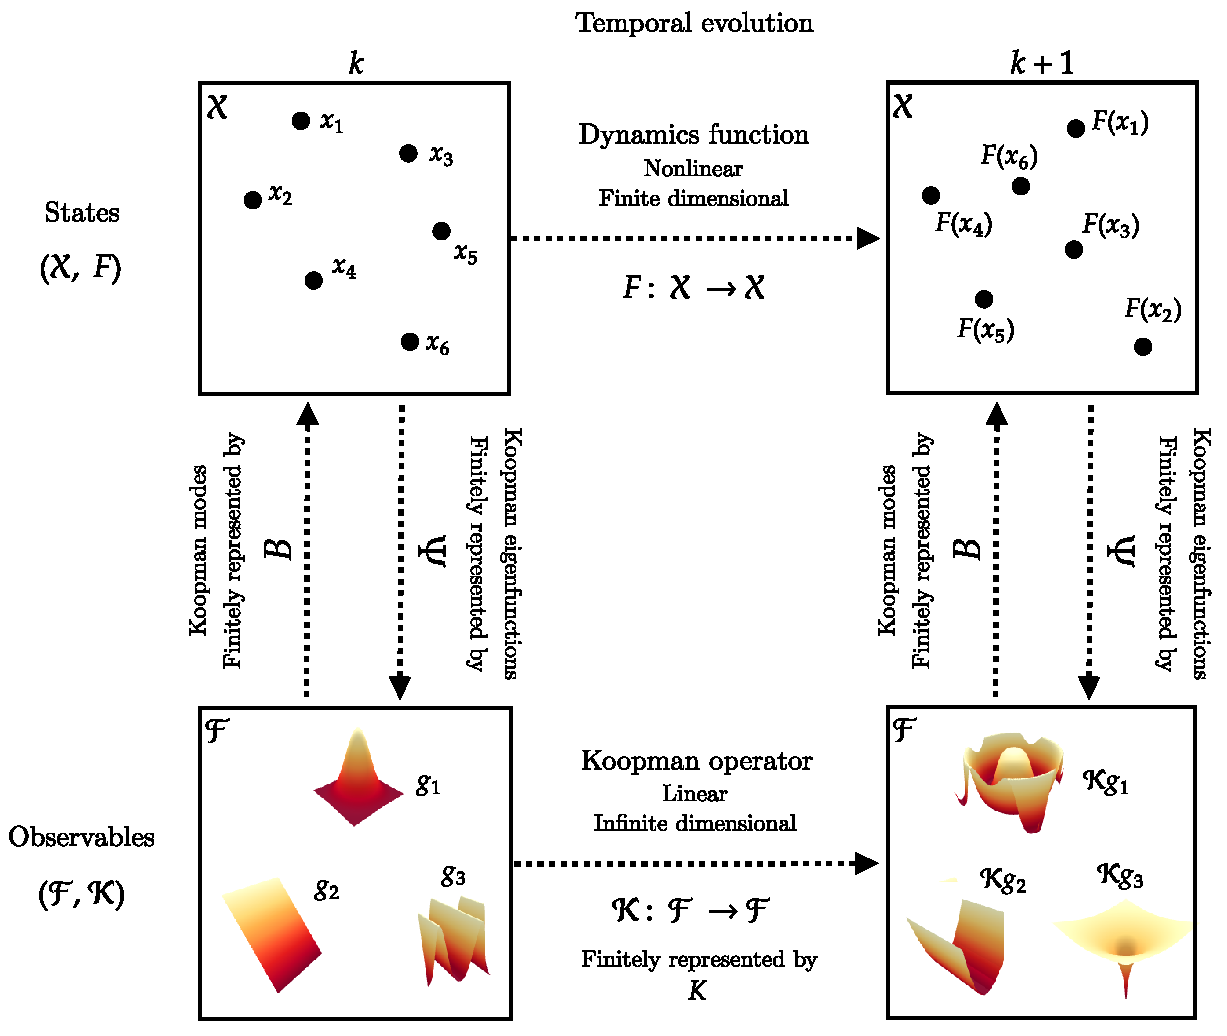
\includegraphics[scale=0.75]{img/content/chapter2/KoopDiag.pdf}
\caption{Diagrama de evolución temporal en dimensión infinita y finita, representando la dinámica mediante el operador de Koopman y sus aproximaciones. Elaboración propia, basado en \cite{Williams2015ADecomposition}.}
\label{fig:KoopDiag}
\end{figure}

\section{Aproximación de rango bajo de matrices}
La dimensión de aproximación del operador de Koopman puede ser muy alta para ciertas aplicaciones, lo que hace que ciertas operaciones se hagan muy inestables si se mantiene el rango original. Es por ello que en muchos contextos se propone bajar el rango de las matrices involucradas vía Descomposición en Valores Singulares (SVD). \\
Primero consideremos el problema de obtener la mejor matriz de rango bajo que aproxima otra matriz dada. La solución de este problema fue dada en \cite{Eckart1936TheRank}, para ello se denota por $r(\mathbf{A})$ el rango de una matriz $\mathbf{A} \in \R^{m \times n}$.

\begin{lema}
	La mejor aproximación de rango \( s \), en términos de la norma de Frobenius, para una matriz \( \mathbf{A} \) de rango \( t \) con \( t \geq s \), es decir, un minimizador global \( \hat{\mathbf{A}}^* \) de
	\[
	\min_{\hat{\mathbf{A}}} \| \mathbf{A} - \hat{\mathbf{A}} \|_F, \quad \text{s.a.} \quad r(\hat{\mathbf{A}}) \leq s
	\]
	viene dada por
	\[
	\hat{\mathbf{A}}^* = P_s (\mathbf{A}) = \mathbf{U} \Sigma_s \mathbf{V}^T,
	\]
	donde \( \Sigma_s \) es la matriz diagonal con los \( s \) valores singulares más grandes de \( \mathbf{A} \) y luego solo $0$, en donde se denota a la SVD de \( \mathbf{A} = \mathbf{U} \Sigma \mathbf{V}^T \).
\end{lema}
\noindent Es con esto que en \cite{Xiang2012OptimalMinimization} se provee una forma cerrada para un problema de regresión lineal en el que se busca que la matriz solución sea de rango bajo también, esto se formula como
\begin{equation}
	\min_{\mathbf{M}} \| \mathbf{Y} - \mathbf{M}\mathbf{X} \|_F, \quad \text{s.a.} \quad r(\mathbf{M}) \leq s
\end{equation}
\begin{prop}
	Sea la SVD de $\mathbf{X} = \mathbf{U} \Sigma \mathbf{V}^T$, con $\textbf{U} \in \R^{m \times m}$, $\mathbf{V} \in \R^{n \times n}$ matrices ortogonales y $\Sigma$ la matriz diagonal con los valores singulares. Luego, el óptimo debe cumplir
	\[
	\mathbf{V}^T \mathbf{M}^* =
	\begin{bmatrix}
		\Sigma_{r(\mathbf{X})}^{-1} P_s(\mathbf{W}_{r(\mathbf{X})}) \\
		\mathbf{a}
	\end{bmatrix},
	\]
	donde $\Sigma_{r(\mathbf{X})}$ es la matriz diagonal con los valores singulares no nulos de $\mathbf{X}$, $\mathbf{W}_{r(\mathbf{X})}$ aquella con las primeras $r(\mathbf{X})$ filas de $\mathbf{W}$, con $\mathbf{W} = \mathbf{U}^T \mathbf{Y}$.
\end{prop}
\noindent Este resultado será importante para poder trabajar matrices de alta dimensionalidad, como ocurre en el caso de EDMD.


% Capítulo 3: Kernel Extended Dynamic Mode Decomposition 
\chapter{Kernel Extended Dynamic Mode Decomposition}
En lo que sigue, se considerarán sistemas de la forma:
\begin{equation}
	\begin{aligned}
		\mathbf{x}_{k+1} &= \mathbf{f}(\mathbf{x}_k, \mathbf{w}_k), \\
		\mathbf{y}_k &= \mathbf{g}(\mathbf{x}_k, \mathbf{v}_k).
	\end{aligned}
	\label{eq:no_lin_dis_chap3}
\end{equation}
En comparación con el problema original, se omitirán explícitamente el tiempo y la entrada (\textit{input}) en la dinámica del sistema. Sin embargo, esto no implica una pérdida de generalidad. Por un lado, el tiempo puede ser incorporado como una variable de estado adicional, de manera que si se define \( \mathbf{x}_{k}^{n+1} = t_k \), entonces la evolución de esta coordenada viene dada por:
\begin{equation*}
    \mathbf{x}_{k+1}^{n+1} = \mathbf{x}_{k}^{n+1} + \Delta t_k,
\end{equation*}
donde \( \Delta t_k \) representa el paso de tiempo en el instante \( k \), el cual, en muchas aplicaciones, se asume constante.

Por otro lado, dado que la entrada \( \mathbf{u}_k \) no se considera una variable de decisión, se asumirá conocida o accesible de manera indefinida, es decir, la secuencia \( \{ \mathbf{u}_k \}_{k \geq 0} \) es completamente observable. En consecuencia, es suficiente con incorporarla como una coordenada adicional en el estado, es decir, \( \mathbf{x}_{k}^{n+1} = \mathbf{u}_k \).

El objetivo de este capítulo es presentar un marco general para el \textit{Kernel Extended Dynamic Mode Decomposition} (kEDMD) que se ajuste a los requerimientos previamente discutidos en la sección anterior. En particular, estos requerimientos incluyen:
\begin{itemize}
    \item La existencia de una función de \textit{lifting forward} que permita realizar un \textit{embedding} en un espacio de dimensión superior.
    \item Un operador que modele la evolución del sistema en tiempo discreto dentro del espacio embebido.
    \item Un operador de reconstrucción que posibilite la recuperación de las variables originales desde el espacio embebido.
    \item La representación de las observaciones en un espacio funcional de dimensión infinita.
\end{itemize}

La metodología propuesta establece una conexión entre los operadores de covarianza introducidos en los preliminares y el operador de Koopman, entendiendo este último como una herramienta más universal y transversal dentro del desarrollo del trabajo.

Finalmente, se enunciará y demostrará un teorema que cuantifica el error de aproximación del operador de Koopman en el contexto de los RKHS. Dicho resultado será utilizado posteriormente y comparado con el demostrado por Philipp et al. \cite{Philipp2024ErrorOperator}. Además, el mismo grupo de investigación ha desarrollado cotas de error en distintos contextos, lo que resulta relevante para futuras extensiones de este trabajo \cite{Philipp2023ErrorFramework, Nuske2023Finite-DataControl, Kohne2024L-errorDecomposition, Harder2024Group-ConvolutionalDecomposition, Philipp2024VarianceOperators, Peitz2025EquivarianceEquations}.

Es importante destacar que todas las construcciones presentadas en este capítulo, junto con el enfoque de formular el operador de Koopman como una herramienta transversal en el contexto de filtrado, así como la integración de cotas de error provenientes de la literatura, constituyen una contribución original de este trabajo.

\section{Operadores de Koopman en RKHS}

Sea $\B_\X$ la $\sigma$-álgebra de Borel definida sobre $\X$ y $\B_{\R^p}$ la correspondiente a $\R^p$. Se introducen las siguientes medidas de probabilidad:  
\[
\begin{aligned}
    \rho_f: \X \times \B_\X \to [0, 1], & \quad \rho_f (\mathbf{x}, A) = \P (\mathbf{f}(\mathbf{x}, \cdot ) \in A ), \\
    \rho_g: \X \times \B_\Y \to [0, 1], & \quad \rho_g(\mathbf{x}, A) = \P (\mathbf{g}(\mathbf{x}, \cdot ) \in A).
\end{aligned}
\]

En este contexto, $\rho_f$ representa la medida inducida por la dinámica del sistema, mientras que $\rho_g$ corresponde a la medida inducida por las observaciones.  
Se asume que el espacio de estados $\X$ es compacto y que existe un conjunto compacto $\Y \subseteq \R^p$ tal que  
\[
\rho_f (\mathbf{x}, \X) = 1, \quad \rho_g (\mathbf{x}, \Y) = 1, \quad \forall \mathbf{x} \in \X.
\]

Sea entonces $\B_\Y$ la $\sigma$-álgebra $\B_{\R^p}$ restringida a $\Y$. Se introduce la siguiente notación diferencial:
\[
\rho_f (\mathbf{x}, dx) = d \rho_f (\mathbf{x}, \cdot)(x), \quad \rho_g (\mathbf{x}, dy) = d \rho_g (\mathbf{x}, \cdot)(y).
\]

Adicionalmente, se consideran funciones de densidad  
\[
p_f : \X \times \X \to \R_+, \quad p_g : \X \times \Y \to \R_+,
\]
tales que, para $\mu_\X$ y $\mu_\Y$ medidas sobre $\X$ y $\Y$, respectivamente, se cumple:
\[
\rho_f (\mathbf{x}, A) = \int_A p_f (\mathbf{x}, y) \, d \mu_\X (y), \quad \rho_g (\mathbf{x}, A) = \int_A p_g (\mathbf{x}, y) \, d \mu_\Y (y).
\]

Bajo este marco, se adoptan las siguientes convenciones:
\begin{itemize}
    \item La variable aleatoria asociada a $\mu_\X$ se denota por $X$.  
    \item La variable aleatoria asociada a $\rho_f$, que describe la evolución de un estado $\mathbf{x}$ tras un paso de la dinámica, se denota por $X^+ \mid \mathbf{x}$.  
    \item La variable aleatoria asociada a $\rho_g$, que modela las observaciones condicionadas a un estado $\mathbf{x}$, se denota por $Y \mid \mathbf{x}$.  
\end{itemize}

\begin{obs}
Un ejemplo concreto de este marco es el siguiente: considérese el caso en que la dinámica del sistema está dada por  
\[
    \mathbf{f}(\mathbf{x}_k, \mathbf{w}_k) = \Tilde{\mathbf{f}}(\mathbf{x}_k) + \mathbf{w}_k,
\]
donde $\mathbf{w}_k \sim \mathcal{N}(0, \mathbf{Q}_k)$, con $\mathbf{Q}_k$ definida positiva, y donde $\mu_\X$ es la medida de Lebesgue en $\X$. En este caso, la medida $\rho_f (\mathbf{x}_k, \cdot)$ sigue una distribución normal:  
\[
    \rho_f (\mathbf{x}_k, \cdot) \sim \mathcal{N}(\Tilde{\mathbf{f}}(\mathbf{x}_k), \mathbf{Q}_k).
\]
    
En consecuencia, la densidad $p_f$ asociada toma la forma  
\[
p_f(x, y) = (2 \pi \det \mathbf{Q}_k )^{-1/2} \exp \left( -\frac{1}{2} (\Tilde{\mathbf{f}}(x) - y)^\top \mathbf{Q}_k^{-1} (\Tilde{\mathbf{f}}(x) - y) \right),
\]
la cual es acotada, incluso si $\Tilde{\mathbf{f}}$ no lo es.  
\end{obs}

Para garantizar la validez de los resultados en \cite{Philipp2024ErrorOperator}, se asumirán las siguientes hipótesis de compatibilidad:
\begin{enumerate}
    \item[a)] Sean $k_\X:\X \times \X \to \R$ y $k_\Y: \Y \times \Y \to \R$ dos \textit{kernels} simétricos, continuos, acotados y semi-definidos positivos. Se denotará por $\H_\X$ y $\H_\Y$ a los RKHS asociados a $k_\X$ y $k_\Y$, respectivamente.
    
    \item[b)] Si $\psi_\X \in L^2(\X)$ y $\psi_\Y \in L^2(\Y)$ satisfacen  
    \[
        \int_{\X \times \X} k_\X(x,y) \psi_\X (x) \psi_\X (y) d \mu_\X (x) d \mu_\X (y) = 0, 
    \]
    \[
        \int_{\Y \times \Y} k_\Y(x,y) \psi_\Y (x) \psi_\Y (y) d \mu_\Y (x) d \mu_\Y (y) = 0, 
    \]
    entonces $\psi_\X = 0$ y $\psi_\Y = 0$ casi seguro.
    
    \item[c)] Si $\psi_\X \in \H_\X$ y $\psi_\Y \in \H_\Y$ son tales que $\psi_\X(x) = 0$ para todo $x \in \X$ $\mu_\X$-casi seguro, y $\psi_\Y(y) = 0$ para todo $y \in \Y$ $\mu_\Y$-casi seguro, entonces $\psi_\X \equiv 0$ y $\psi_\Y \equiv 0$.
    
    \item[d)] Se asumen las siguientes relaciones entre $\rho_f$ y $\rho_g$ con respecto a $\mu_\X$ y $\mu_\Y$:
    \[
        \int_\X \rho_f (x, A_\X) d\mu_\X (x) \leq L_\X \mu_\X (A_\X), \quad \forall A_\X \in \B_\X,
    \]
    \[
        \int_\X \rho_g (x, A_\Y) d\mu_\X (x) \leq L_\Y \mu_\Y (A_\Y), \quad \forall A_\Y \in \B_\Y.
    \]
\end{enumerate}

Un ejemplo de un \textit{kernel} que satisface las hipótesis a) y b) es el \textit{kernel} de Matérn. La propiedad a) es garantizada por los resultados presentados en la sección anterior, mientras que la propiedad b) se deriva de la universalidad del \textit{kernel} en $L^2$. 

La hipótesis c) se satisface si $\mu_\X$ y $\mu_\Y$ tienen densidad respecto a la medida de Lebesgue, y la hipótesis d) se cumple en el caso estocástico cuando las funciones $p_f$ y $p_g$ son acotadas. 

\begin{prop}
    Si $p_f \in L^{\infty} (\X \times \X)$ y $p_g \in L^{\infty} (\X \times \Y)$, entonces:
    \[
        \int_\X \rho_f (x, A) d\mu_\X (x) \leq L_\X \mu_\X (A), \quad \int_\X \rho_g (x, A) d\mu_\X (x) \leq L_\Y \mu_\Y (A),
    \]
    donde:
    \[
        L_\X = \mu_\X (\X) \| p_f \|_\infty, \quad L_\Y = \mu_\X (\X) \| p_g \|_\infty.
    \]
\end{prop}

\begin{proof}
    Para $\rho_f$, se tiene que:
    \[
        \begin{aligned}
            \int_\X \rho_f (x, A) d\mu_\X (x) &= \int_\X \int_A d \rho_f (x, \cdot) (y) d \mu_\X (x) \\
            &= \int_\X \int_A p_f (x, y) d \mu_\X (y) d \mu_\X (x) \\
            &\leq \| p_f \|_\infty \int_\X \int_A d \mu_\X (y) d \mu_\X (x) \\ 
            &= \| p_f \|_\infty \mu_\X (\X) \mu_\X (A) \\
            &= L_\X \mu_\X (A).
        \end{aligned}
    \]
Para $\rho_g$, de manera similar, se tiene que:
    \[
        \begin{aligned}
            \int_\X \rho_g (x, A) d\mu_\X (x) &= \int_\X \int_A d \rho_g (x, \cdot) (y) d \mu_\X (x) \\
            &= \int_\X \int_A p_g (x, y) d \mu_\Y (y) d \mu_\X (x) \\
            &\leq \| p_g \|_\infty \int_\X \int_A d \mu_\Y (y) d \mu_\X (x) \\ 
            &= \| p_g \|_\infty \mu_\X (\X) \mu_\Y (A) \\
            &= L_\Y \mu_\Y (A).
        \end{aligned}
    \]
\end{proof}
En el caso en que la dinámica y la observación sean deterministas, esto es equivalente a que $\mathbf{f}(\mathbf{x}, \mathbf{w}) = \Tilde{\mathbf{f}}(\mathbf{x})$ y $\mathbf{g}(\mathbf{x}, \mathbf{v}) = \Tilde{\mathbf{g}}(\mathbf{x})$, con lo que $\rho (x, \cdot) = \delta_{\Tilde{\mathbf{f}}(x)}(\cdot)$ y $\xi (x, \cdot) = \delta_{\Tilde{\mathbf{g}}(x)}(\cdot)$. En este caso, es necesario asumir mayor regularidad sobre las funciones involucradas.

\begin{prop}
    Si $\rho (x, \cdot) = \delta_{\Tilde{\mathbf{f}}(x)}(\cdot)$ y $\xi (x, \cdot) = \delta_{\Tilde{\mathbf{g}}(x)}(\cdot)$, y $\tilde{\mathbf{f}}$ y $\tilde{\mathbf{g}}$, según corresponda, son difeomorfismos de clase $C^1$ tales que:
    \begin{equation*}
        \inf_{x \in \X} \left | \det ( D \tilde{\mathbf{f}} (x) ) \right | > 0, \quad \inf_{x \in \X} \left | \det ( D \tilde{\mathbf{g}} (x) ) \right | > 0,
    \end{equation*}
    entonces:
    \begin{equation*}
        \int_\X \rho_f (x, A) d\mu (x) \leq L_f \mu (A), \quad \int_\X \rho_g (x, A) d\mu_\X (x) \leq L_g \mu_\Y (A),
    \end{equation*}
    con:
    \begin{equation*}
        L_f = \left \| \det ( D \tilde{\mathbf{f}}^{-1} ) \right \|_\infty, \quad L_g = \left \| \det ( D \tilde{\mathbf{g}}^{-1} ) \right \|_\infty.
    \end{equation*}
\end{prop}
\begin{proof}

La demostración sigue un razonamiento similar al expuesto en \cite{Kohne2024L-errorDecomposition}. Para un conjunto $A \in \B$, se observa que $\rho_f (x, A) = \delta_{\Tilde{\mathbf{f}}(x)}(A) = \mathds{1}_A (\Tilde{\mathbf{f}}(x))$. Por lo tanto:
    \begin{equation*}
        \begin{aligned}
            \int_\X \rho_f (x, A) d\mu (x) &= \int_\X \mathds{1}_A (\Tilde{\mathbf{f}}(x)) d \mu_\X (x) \\
            &= \int_\X \mathds{1}_A (x) \left | \det ( D \Tilde{\mathbf{f}}^{-1}(x) ) \right | d \mu_\X (x) \\
            &\leq \left \| \det ( D \Tilde{\mathbf{f}}^{-1} ) \right \|_\infty \int_\X \mathds{1}_A (x) d\mu_\X (x) \\
            &= \left \| \det ( D \Tilde{\mathbf{f}}^{-1} ) \right \|_\infty \mu_\X (A) \\
            &= L_f \mu_\X (A).
        \end{aligned}
    \end{equation*}
    El caso de $\rho_g$ se demuestra de manera análoga.
\end{proof}

A continuación, se presentan las definiciones de los operadores de Koopman estocásticos para la dinámica y la observación, adaptados al caso en que se disponen de las funciones $p_f$ y $p_g$ como densidades.

\begin{defn}[Operador de Koopman estocástico para la dinámica, tiempo discreto]
	Se define el operador asociado a $\mathbf{f}$ como $\U : L^2(\X) \to L^2(\X)$, dado por:
	\begin{equation*}
		[\U h](x) = \E [h (\mathbf{f} (x, \cdot) )]  = \int_\X h(x') \rho_f (x, dx') = \int_\X h(x') p_f (x, x') d \mu_\X (x').
	\end{equation*}
\end{defn}

\begin{defn}[Operador de Koopman estocástico para la observación]
    Se define el operador asociado a $\mathbf{g}$ como $\G : L^2(\Y) \to L^2(\X)$, dado por:
	\begin{equation*}
		[\G h](x) = \E [h (\mathbf{g} (x, \cdot) )]  = \int_\Y h(y) \rho_g (x, dy) = \int_\Y h(y) p_g (x, y) d \mu_\Y (y).
	\end{equation*}
\end{defn}

Se introduce el operador de Perron-Frobenius, que posteriormente mostrará no solo una relación con el operador de Koopman, sino también la dinámica subyacente. A continuación, se presentan sus definiciones en el contexto estocástico para la dinámica y la observación.

\begin{defn}[Operador de Perron-Frobenius estocástico para la dinámica]
	Se define el operador asociado a $\mathbf{f}$ como $\mathcal{P}_\mathbf{f} : L^2(\X) \to L^2(\X)$, dado por:
	\begin{equation*}
		[\mathcal{P}_\mathbf{f} h](x) = \int_\X h(x') p_f (x', x) d \mu_\X (x').
	\end{equation*}
\end{defn}

\begin{defn}[Operador de Perron-Frobenius estocástico para la observación]
	Se define el operador asociado a $\mathbf{g}$ como $\mathcal{P}_\mathbf{g} : L^2(\X) \to L^2(\Y)$, dado por:
	\begin{equation*}
		[\mathcal{P}_\mathbf{g} h](x) = \int_\X h(y) p_g (y, x) d \mu_\X (y).
	\end{equation*}
\end{defn}

Dado que los operadores $\mathcal{P}_\mathbf{f}$ y $\mathcal{P}_\mathbf{g}$ están definidos en términos de las funciones de densidad $p_f$ y $p_g$, se cumple que:
\begin{equation*}
	\U^* = \mathcal{P}_\mathbf{f}, \quad \G^* = \mathcal{P}_\mathbf{g},
\end{equation*}
donde $\U^*$ y $\G^*$ denotan los operadores adjuntos de $\U$ y $\G$, respectivamente.

En este punto se tomará la elección de tomar $k_\Y$ como el \textit{kernel} dado por el producto interno en $\R^p$, con lo que su \textit{feature map} canónico es la función identidad en dicho espacio y $\H_\Y = \R^p$. En lo que sigue, se retomarán las definiciones de la sección anterior, pero específicas en este contexto.

\begin{defn}[Feature map canónico]
	Se definen los \textit{feature maps} canónicos de los \textit{kernels} $\Phi_\X : \X \to \H_\X$ y $\Phi_\Y : \Y \to \R^p$ como:
	\begin{equation*}
		\Phi_\X (x) = k_\X (x, \cdot), \quad \Phi_\Y (y) = k_\Y (y, \cdot) = \langle y, \cdot \rangle.
	\end{equation*}
\end{defn}

\begin{defn}
	Para $x_1, x_2 \in \X$ y $y_1, y_2 \in \Y$, se definen los operadores de rango 1 $C_{x_1,x_2} : \H_\X \to \H_\X$, $C_{y_1,y_2} : \R^p \to \R^p$ y $C_{y_1,x_1} : \H_\X \to \R^p$ como:
	\begin{equation*}
		C_{x_1, x_2} \psi = \langle \psi, \Phi_\X (x_2) \rangle \Phi_\X (x_1) = \psi (x_2) \Phi_\X (x_1),
	\end{equation*}
	\begin{equation*}
		C_{y_1, y_2} \psi = \langle \psi, \Phi_\Y (y_2) \rangle \Phi_\Y (y_1) = \psi (y_2) \Phi_\Y (y_1),
	\end{equation*}
	\begin{equation*}
		C_{y_1, x_1} \psi = \langle \psi, \Phi_\X (x_1) \rangle \Phi_\Y (y_1) = \psi (x_1) \Phi_\Y (y_1).
	\end{equation*}
\end{defn}

\begin{defn}[Operadores de covarianza]
	Se definen los operadores de covarianza 
    \begin{equation*}
        C_X : \H_\X \to \H_\X, \quad C_Y : \R^p \to \R^p
    \end{equation*} 
    como:
	\begin{equation*}
		C_X \psi = \int_\X \langle \psi, \Phi_\X (x) \rangle \Phi_\X (x) d \mu_\X (x) = \int_\X [\Phi_\X (x) \otimes \Phi_\X (x)] \psi d \mu_\X (x),
	\end{equation*}
	\begin{equation*}
		C_Y \psi = \int_\Y \langle \psi, \Phi_\Y (y) \rangle \Phi_\Y (y) d \mu_\Y (y) = \int_\Y [\Phi_\Y (y) \otimes \Phi_\Y (y)] \psi d \mu_\Y (y).
	\end{equation*}
\end{defn}

\begin{defn}[Operadores de covarianza cruzada]
    El operador de covarianza cruzada asociado a la dinámica es $C_{X X^+} : \H_\X \to \H_\X$, dado por:
	\begin{equation*}
		C_{X X^+} \psi = \int_\X \int_\X \langle \psi, \Phi_\X (y) \rangle \Phi_\X (x) d\rho_f (x, \cdot)(y) d \mu_\X (x).
	\end{equation*}
    
    El operador de covarianza cruzada asociado a la observación es $C_{\Y \X} : \H_\X \to \R^p$, dado por:
	\begin{equation*}
		C_{Y X} \psi = \int_\X \int_\Y \langle \psi, \Phi_\X (x) \rangle \Phi_\Y (y) d\rho_g (x, \cdot)(y) d \mu_\X (x).
	\end{equation*}
\end{defn}

\begin{defn}[Operadores de \textit{embedding} condicional]   
    Se definen los operadores de \textit{embedding} condicional $C_{X^+ | X} : \H_\X \to \H_\X$ y $C_{Y | X} : \H_\X \to \R^p$ como:
	\begin{equation*}
		C_{X^+ | X} = C_{X^+ X} C_X^{-1}, \quad C_{Y | X} = C_{Y X} C_X^{-1}.
	\end{equation*}
\end{defn}

Finalmente, será necesario asumir que $\U \H_\X \subset \H_\X$ y $\G \R^p \subset \H_\X$. Esto se cumple, por ejemplo, si $\H_\X$ es un espacio de Sobolev, como en el caso de que $k_\X$ sea un \textit{kernel} de Matérn. En este contexto, Köhne et al. \cite{Kohne2024L-errorDecomposition} prueban que esto se tiene cuando las funciones asociadas son difeomorfismos. A efectos de este trabajo fue necesario extender dicho resultado al caso estocástico, lo que se refleja en los siguientes dos resultados.

\begin{prop}[Invarianza Sobolev para Koopman]
	Sea $s \geq 0$, $k =\lceil s \rceil $ y $H^s(\X)$ el espacio de Sobolev sobre $\X$. Si $p_f \in C^{k,k} (\X \times \X)$ y $p_g \in C^{k,k} (\X \times \Y)$, entonces:
	\begin{equation*}
		\U H^s (\X) \subseteq H^s (\X), \quad \G \R^p \subseteq H^s (\X).
	\end{equation*}
\end{prop}

\begin{proof}
	Sea $m \in \N$, $m \leq k$ y $|\alpha| = m$ un multiíndice. Para $h \in H^m (\X)$, por el teorema de la convergencia dominada:
	\begin{equation*}
		\partial^\alpha_x (\U h)(x) = \int_\X h(y) \partial^\alpha_x p_{\mathbf{f}} (x, y) d \mu_\X (y).
	\end{equation*}
	Por lo tanto:
	\begin{equation*}
		\begin{aligned}
			\| \partial^\alpha_x (\U h) \|_{L^2}^2 & \leq \int_\X \int_\X h(y)^2 \partial^\alpha_x p_{\mathbf{f}} (x, y)^2 d \mu_\X (y) d \mu_\X (x) \\
			& \leq \| \partial^\alpha_x p_{\mathbf{f}} \|_{C^{k,k}} \mu_\X (\X) \int_\X h(y)^2 d \mu_\X (y) \\
			& \leq \| \partial^\alpha_x p_{\mathbf{f}} \|_{C^{k,k}} \mu_\X (\X) \| h \|_{\H^k (\X)}^2.
		\end{aligned}
	\end{equation*}
	Así, se concluye que $\U h \in H^m (\X)$ y:
	\begin{equation*}
		\| \U \|_{H^m \to H^m} \leq \mu_\X (\X) \sum_{|\alpha| \leq k} \| \partial^\alpha_x p_{\mathbf{f}} \|_{C^{k,k}}.
	\end{equation*}
        Es así que
        \[
        \U H^m \subseteq H^m, \, \forall m \in \{ 0, \dots, k \}.
        \]

        De un resultado de interpolación \cite{Brenner2008TheMethods} se sabe que para $\ell \in [0, k]$ real se tiene que $H^\ell$ resulta ser la interpolación entre $H^0 = L^2$ y $H^k$, esto es, para $\theta \in [0, 1]$ se tiene
        \[
        H^\ell = [H^0, H^k]_\theta = H^{(1-\theta) \cdot 0 + \theta \cdot k} = H^{\theta k}.
        \]
        Con ello, se tiene que
        \[
        \U H^\ell \subseteq H^\ell, \, \forall \ell \in [0, k],
        \]
        en particular, se tiene para todo $\ell \in [0, s]$ dado que $k = \lceil s \rceil$. El caso de $\G$ se demuestra de manera análoga.
\end{proof}

Esto lleva directamente a un resultado para la invarianza de Koopman a través de ciertos RKHS.

\begin{cor} 
\label{cor:inv_koop}
    Si $\H_\X$ es equivalente a un espacio de Sobolev $H^s$ y $p_f \in C^{k,k} (\X \times \X)$ y $p_g \in C^{k,k} (\X \times \Y)$, entonces:
	\begin{equation*}
		\U H^s (\X) \subseteq H^s (\X), \quad \G \R^p \subseteq H^s (\X).
	\end{equation*}
\end{cor}

Bajo la condición de invarianza anterior, ya fue visto en \cite{Philipp2023ErrorFramework} que el operador de Koopman se relaciona de manera directa con los operadores de covarianza en RKHS. Pero, en este contexto se explotará la forma del operador en conjunto con las propiedades de los adjuntos para probar un resultado similar, lo que será de mucha utilidad posteriormente.

\begin{teo}
\label{teo:cov_koop_equiv}
    Si 
    \begin{equation*}
        \U \H_\X \subset \H_\X, \quad \G \R^p \subset \H_\X,
    \end{equation*}
    entonces se cumple que
    \begin{equation*}
        C_{X^+ X} C_X^{-1} = C_{X^+ | X} = \U^* = \mathcal{P}_\mathbf{f}, \quad C_{Y | X} = \G^* = \mathcal{P}_\mathbf{g}.
    \end{equation*}
\end{teo}

\begin{proof}
Primero, un manejo algebraico permite establecer la siguiente relación:
\begin{equation*}
    \begin{aligned}
        C_{X X^+} \psi &= \int_\X \int_\X [\Phi_\X (x) \otimes \Phi_\X (y)] \psi \, d\rho_f (x, \cdot) (y) \, d\mu_\X (x) \\
        &= \int_\X \int_\Y \psi(y) \Phi_\X (x) \, d\rho_f (x, \cdot) (y) \, d\mu_\X (x) \\
        &= \int_\X (\U \psi)(x) \Phi_\X (x) \, d\mu_\X (x). \\
    \end{aligned}
\end{equation*}
En la última relación obtenida se obtiene el operador de rango 1 que representa al producto de Kronecker, visto en la definición \ref{def:kronecker}
\begin{equation*}
    \begin{aligned}
        C_{X X^+} \psi &= \int_\X [\Phi_\X (x) \otimes \Phi_\X (x)] (\U \psi) \, d\mu_\X (x) \\
        &= C_X \U \psi.
    \end{aligned}
\end{equation*}

Por tanto, se tiene que 
\begin{equation*}
    C_{X X^+} = C_X \U.
\end{equation*}
Notando que
\begin{equation*}
    C_X = \mathbb{E}[\Phi_\X (X) \otimes \Phi_\X (X)], \quad
    C_{X X^+} = \mathbb{E}[\Phi_\X (X) \otimes \Phi_\X (X^+)]
\end{equation*}
y que 
\begin{equation*}
    (\Phi_\X (X) \otimes \Phi_\X (X^+))^* = \Phi_\X (X^+) \otimes \Phi_\X (X),
\end{equation*}
se deduce que 
\begin{equation*}
    C_X^* = C_X \quad \text{y} \quad C_{X X^+}^* = C_{X^+X}.
\end{equation*}

Así, resulta que 
\begin{equation*}
    C_{X^+X} C_X^{-1} = \U^*,
\end{equation*}
con lo cual se concluye 
\begin{equation*}
    C_{X^+X} C_X^{-1} = C_{X^+ | X} = \U^* = \mathcal{P}_\mathbf{f}.
\end{equation*}
De forma análoga, se demuestra que
\begin{equation*}
    C_{Y | X} = \G^* = \mathcal{P}_\mathbf{g}.
\end{equation*}

Estas igualdades deben entenderse cuidadosamente y están bien definidas bajo la condición de que $C_X$ sea inyectivo \cite{Fukumizu2013KernelKernels}, lo que se verá con mayor profundidad después.
\end{proof}

\begin{obs}
    El hecho de que el operador de el operador de \textit{embedding} de la distribución condicional sea el adjunto del operador de Koopman, y no el operador de Koopman en sí mismo, está relacionado con algo ya visto por Gerlach et al., en donde indican que el operador de Koopman genera una dinámica de funciones y el operador de Perron-Frobenius una de distribuciones. Esto se explica mejor en la figura \ref{fig:koopman_exp}.
    \begin{figure}[h!]
        \centering
        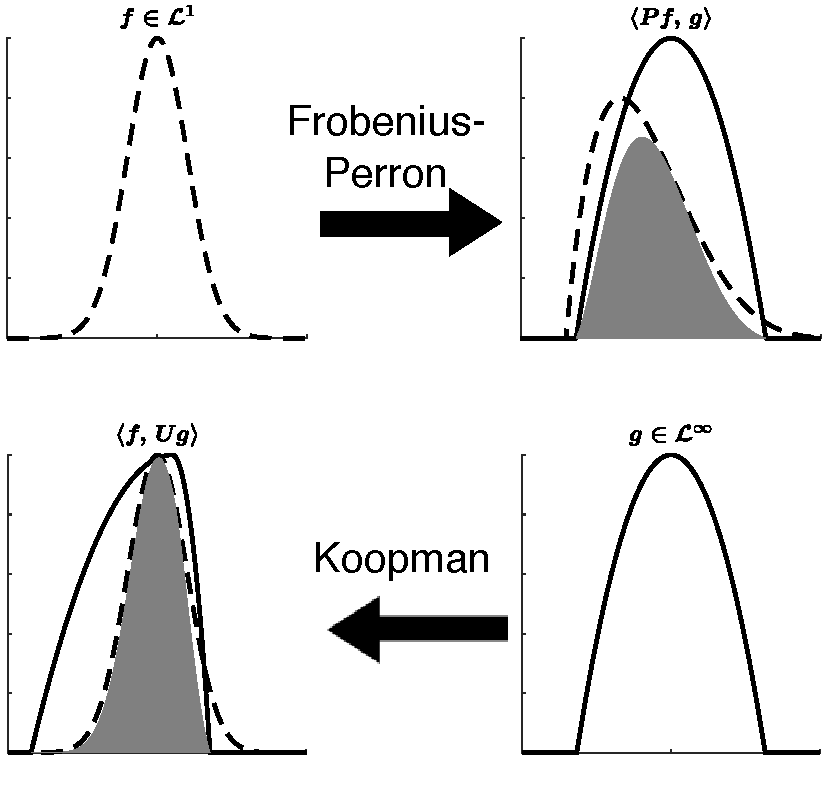
\includegraphics[width=0.5\linewidth]{img/content/chapter3/koopman_exp.pdf}
        \caption{Diagrama explicativo de la relación entre el operador de Koopman y Perron-Frobenius, obtenido de \cite{Gerlach2020TheSystems}, a su vez adaptado de \cite{Leonard2019ProbabilisticAirdrop}.}
        \label{fig:koopman_exp}
    \end{figure}
\end{obs}
Notar que, una vez realizado el \textit{embedding} a dimensión infinita de las distribuciones de probabilidad del problema, es necesario regresar al espacio de dimensión original. Por ello, se introduce un nuevo operador de Koopman que actuará como un operador de \textit{lifting back}.

Sea $\Tilde{k}_\X: \X \times \X \to \R$ el \textit{kernel} definido a partir del producto interno, con lo cual su \textit{feature map} canónico $\phi : \X \to \R^n$ está dado por la función identidad. Esto es:
\begin{equation*}
    \Tilde{k}_\X (x, y) = x^\top y, \quad \phi (x) = x.
\end{equation*}
Entonces, el operador de covarianza cruzada asociado a $X$ y a los \textit{embeddings} entre $\H_\X$ y $\R^n$, este último considerado como el RKHS asociado a $\Tilde{k}_\X$, $C_{X|X} : \H_\X \to \R^n$, debe satisfacer
\begin{equation*}
    C_{X|X} \Phi_\X (\mathbf{x}) = \mathbb{E} [\phi (X) | X = \mathbf{x}] = \mathbb{E}[ X | X = \mathbf{x}] = \mathbf{x}.
\end{equation*}

De este modo, en virtud del teorema \ref{teo:cov_koop_equiv}, se concluye que existe un operador de Koopman $\B : \R^n \to \H_\X$ tal que $C_{X|X} = \B^*$, al cual denominaremos operador de \textit{lifting back}. Este operador permitirá regresar al espacio original desde un espacio de dimensión mayor.

\section{Aproximación de operadores de Koopman}

En esta sección se describe el proceso de aproximación de los operadores de Koopman relacionados con la dinámica, observación y reconstrucción. Para ello, se consideran \( N \) puntos, representados como \( \{ x_i \}_{i=1}^N \sim \mu_\X^N \), y conjuntos de puntos adicionales \( \{ x^+_i \}_{i=1}^N \) y \( \{ y_i \}_{i=1}^N \), generados bajo las siguientes distribuciones:
\begin{equation*}
    x^+_i \sim \rho_f (x_i, \cdot), \quad y_i \sim \rho_g (x_i, \cdot), \quad i = 1, \dots, N.
\end{equation*}
Se define el espacio:
\begin{equation*}
    \H_{\X, N} = \text{span} \{\Phi_\X (x_i) : i = 1, \dots, N \},
\end{equation*}
cuya base canónica está dada por \( \{\Phi_\X (x_i) : i = 1, \dots, N \} \).

Se introducen las siguientes matrices:
\begin{equation*}
    \mathbf{X} = (x_{1} | \dots | x_N), \quad \mathbf{X}^+ = (x_{1}^+ | \dots | x_N^+), \quad \mathbf{Y} = (y_1 | \dots | y_N),
\end{equation*}
\begin{equation*}
    \Phi_N (\mathbf{X}) = (k_\X(x_i, x_j))_{i,j = 1}^N, \quad \Phi_N (\mathbf{X}^+) = (k_\X(x_i, x^+_j))_{i,j = 1}^N.
\end{equation*}
Con base en estas definiciones, se introducen los operadores:
\begin{equation*}
    C_{X}^N : \H_{\X, N} \to \H_{\X, N}, \quad C_{XX^+}^N : \H_{\X, N} \to \H_{\X, N}, \quad 
\end{equation*}
\begin{equation*}
    C_{XY}^N : \R^p \to \H_{\X, N}, \quad C_{XX}^N : \R^n \to \H_{\X, N}.
\end{equation*}
definidos como
\[
C_X^N = \frac{1}{N} \sum_{j=1}^N \Phi_\X (x_j) \otimes \Phi_\X (x_j), \quad C_{XX^+}^N = \frac{1}{N} \sum_{j=1}^N \Phi_\X (x_j) \otimes \Phi_\X (x_j^+)
\]
\[
C_{XY}^N = \frac{1}{N} \sum_{j=1}^N \Phi_\X (x_j) \otimes \Phi_\Y (y_j), \quad C_{XX}^N = \frac{1}{N} \sum_{j=1}^N \Phi_\X (x_j) \otimes \phi (x_j)
\]
Entonces las acciones de estos operadores viene dada por
\begin{equation*}
    C_{X}^N \Phi_\X (x_i) = \frac{1}{N} \sum_{j = 1}^N k_\X(x_i, x_j) \Phi_\X (x_j), \quad C_{XX^+}^N \Phi_\X (x_i) = \frac{1}{N} \sum_{j = 1}^N k_\X(x_i, x_j^+) \Phi_\X (x_j),
\end{equation*}
\begin{equation*}
        C_{XY}^N \Phi_\Y (y_i) = \frac{1}{N} \sum_{j = 1}^N k_\Y (y_i, y_j) \Phi_\X (x_j), \quad C_{XX}^N \phi (x_i) = \frac{1}{N} \sum_{j = 1}^N \langle x_i, x_j \rangle \Phi_\X (x_j).
\end{equation*}
Estos operadores están representados mediante las matrices \( \Phi_N (\mathbf{X}) \), \( \Phi_N (\mathbf{X}^+) \), \( \mathbf{Y} \) y \( \mathbf{X} \), respectivamente. A continuación, se definen los operadores:
\begin{equation*}
    \U_N : \H_{\X, N} \to \H_{\X, N}, \quad \G_N : \R^p \to \H_{\X, N}, \quad \B_N : \R^n \to \H_{\X, N},
\end{equation*}
los cuales están representados por las siguientes matrices:
\begin{equation*}
    \mathbf{U}_N = (\Phi_N (\mathbf{X}))^{-1} \Phi_N (\mathbf{X}^+)^\top,
\end{equation*}
\begin{equation*}
    \mathbf{G}_N = (\Phi_N (\mathbf{X}))^{-1} \mathbf{Y}^\top,
\end{equation*}
\begin{equation*}
    \mathbf{B}_N = (\Phi_N (\mathbf{X}))^{-1} \mathbf{X}^\top.
\end{equation*}
es decir,
\begin{equation*}
    \U_N = (C_X^N)^{-1} C_{XX^+}^N,
\end{equation*}
\begin{equation*}
    \G_N = (C_X^N)^{-1} C_{XY}^N,
\end{equation*}
\begin{equation*}
    \B_N = (C_X^N)^{-1} C_{XX}^N.
\end{equation*}
El algoritmo \ref{alg:kEDMD} se deja el detalle para poder aplicar \textit{kernel} Extended Dynamic Mode Decomposition en el ámbito computacional.

\begin{algorithm}
\caption{kEDMD($\mu_\X$, $\rho_f$, $\rho_g$, $k$, $N$)}\label{alg:kEDMD}
\begin{algorithmic}[1]
\State \textbf{Entrada:} $\mu_\X$ medida de probabilidad asociada al estado, $\rho_f$ medida de probabilidad asociada a la dinámica, $\rho_g$ medida de probabilidad asociada a la observación, $\mathbf{k}: \X \times \X \to \R$ un \textit{kernel} semidefinido positivo, $N$ dimensión de aproximación de Koopman.
\State \textbf{Salida:} $\mathbf{U}_N \in \R^{N \times N}$ aproximación del operador de Koopman, $\mathbf{\Phi}_N: \X \to \R^{N}$ función de \textit{lifting forward}, $\mathbf{G}_N \in \R^{p \times N}$ matriz de linealización de la observación y $\mathbf{B}_N \in \R^{n \times N}$ matriz de \textit{lifting back}.
\State $x \sim \mu_\X, \, i = 1, \dots, N$ \Comment{$N$ muestras independientes \textit{sampleadas} desde $\mu_\X$}
\State $x_i^+ \gets \rho_f(x_i, \cdot), \, i = 1, \dots, N$ \Comment{$N$ muestras de la dinámica}
\State $y_i \gets \rho_g(x_i, \cdot), \, i = 1, \dots, N$ \Comment{$N$ muestras de la observación}
\State $\Phi_N (\cdot) \gets k(\mathbf{X}, \cdot)$
\Comment{Función de \textit{lift forward}}
\State $\Phi_N (\mathbf{X}) \gets (\mathbf{k}(x_i, x_j))_{i,j=1}^{N}$
\State $\Phi_N (\mathbf{X}^+) \gets (\mathbf{k}(x_i, x_j^+))_{i,j=1}^{N}$
\State $\mathbf{U}_N \gets \Phi_\X (\mathbf{X})^{-1}\Phi_\X (\mathbf{X}^+)^T$
\Comment{Aproximación del operador de Koopman}
\State $\mathbf{G}_N \gets \Phi_\X (\mathbf{X})^{-1} \mathbf{Y}^T$
\Comment{Aproximación del operador de observación}
\State $\mathbf{B}_N \gets \Phi_\X (\mathbf{X})^{-1} \mathbf{X}^T$
\Comment{Matriz de \textit{lift back}}
\end{algorithmic}
\end{algorithm}

Por otra parte, se definen las siguientes normas asociadas al \textit{kernel} \( k_\X \):
\begin{equation*}
    \| k_\X \|_1 = \int_\X k_\X (x,x) d \mu_\X (x), \quad \| k_\X \|_\infty = \sup_{x \in \X} k_\X (x,x),
\end{equation*}
las cuales son finitas en el caso del \textit{kernel} de Matérn. En lo que sigue se probará una cota de error para kEDMD. Para ello primero es necesario ver que algunos de los operadores se pueden extender a $\H_\X$.

\begin{prop}
    Los operadores $C_X^N$ y $C_{XX^+}^N$ se pueden extender como operadores de $\H_\X$ en $ \H_{\X, N}$ de manera continua.
\end{prop}

\begin{proof}
    Sea $\psi \in \H_\X$ y $\varepsilon > 0$ luego por Moore-Aronszajn existen $\{ \Tilde{x}_j \}_{j=1}^m$ tales que
    \[
    \psi_m = \sum_{j=1}^m \alpha_j \Phi_\X (\Tilde{x}_j)
    \]
    cumple $\psi_m \in \H_{\X, m} := \text{span}(\{ \Phi_\X (\Tilde{x}_j), \, j=1,\dots,m \})$ y $\| \psi - \psi_m \| \leq \varepsilon$. Primero se extienden los operadores a espacios finitamente generados como $\H_{\X, m}$, para ello se hace uso de la acción de estos sobre $\Phi_\X (x_i)$, quedando
    \[
    C_X \psi_m =
    \frac{1}{N} \sum_{i=1}^m \alpha_i \sum_{j = 1}^N k_\X(\Tilde{x}_i, x_j) \Phi_\X (x_j), \quad C_{XX^+} \psi_m =
    \frac{1}{N} \sum_{i=1}^m \alpha_i \sum_{j = 1}^N k_\X(\Tilde{x}_i, x_j^+) \Phi_\X (x_j).
    \]
    Entonces se extienden a $\H_\X$ como
    \[
    C_X \psi = \lim_{m \to \infty} C_X \psi_m, \quad C_{XX^+} \psi = \lim_{m \to \infty} C_{XX^+} \psi_m,
    \]
    de forma que
    \[
    C_X \psi =
    \frac{1}{N} \sum_{i \geq 1} \alpha_i \sum_{j = 1}^N k_\X(\Tilde{x}_i, x_j) \Phi_\X (x_j), \quad C_{XX^+} \psi =
    \frac{1}{N} \sum_{i \geq 1} \alpha_i \sum_{j = 1}^N k_\X(\Tilde{x}_i, x_j^+) \Phi_\X (x_j).
    \]
    Con ello basta ver que está definido de manera continua
    \[
    \begin{aligned}
        \| C_X \psi \|^2 & \leq \frac{1}{N^2} \sum_{i \geq 1} \sum_{j=1}^N \alpha_i^2 k(\Tilde{x}_i, x_j)^2 \| \Phi_\X (x_j) \|^2 \\
        & \leq \frac{\| k \|_\infty^2}{N^2} \| \alpha \|_{\ell^2} \sum_{j=1}^N k(x_j, x_j) \\
        & \leq \frac{\| k \|_\infty^2}{N^2} \| \psi \|_{\H_\X} \sum_{j=1}^N k(x_j, x_j). \\
    \end{aligned}
    \]
    Análogamente
    \[
    \| C_{XX^+} \psi \| \leq \frac{\| k \|_\infty^2}{N^2} \| \psi \|_{\H_\X} \sum_{j=1}^N k(x_j, x_j),
    \]
    con lo que los operadores se extienden de manera continua.
\end{proof}

Una desigualdad que será clave es la desigualdad de Hoeffding, que es corolario de un teorema asociado a martingalas, probado por Pinelis en 1994.

\begin{teo}[\cite{Pinelis1994OptimumSpaces} Teorema 3.5]
Sea $(S_k)_{k \in \mathbb{N}}$ una sucesión de martingalas con valores en un espacio de Hilbert real separable $H$ tal que 
\[
\sum_{k=1}^\infty \operatorname{ess\,sup} \|S_k - S_{k-1}\|_H^2 \leq C^2
\]
para alguna constante $C^2 > 0$. Entonces, para todo $\varepsilon > 0$, se tiene
\[
\mathbb{P} \left( \sup_{k \in \mathbb{N}} \|S_k\|_H \geq \varepsilon \right) \leq 2 \exp \left( -\frac{\varepsilon^2}{2C^2} \right).
\]
\end{teo}

\begin{cor}[Desigualdad de Hoeffding en espacios de Hilbert]
Sean $\xi_1, \dots, \xi_n$ variables aleatorias independientes en un espacio de Hilbert separable $H$ tales que $\mathbb{P}$-c.t.p. $\|\xi_i\|_H \leq M$ y $\mathbb{E}[\xi_i] = 0$ para todo $1 \leq i \leq n$. Entonces, para todo $\varepsilon > 0$, se tiene
\[
\mathbb{P} \left( \left\| \frac{1}{n} \sum_{i=1}^n \xi_i \right\|_H \geq \varepsilon \right) \leq 2 \exp \left( -\frac{n\varepsilon^2}{2M^2} \right).
\]
\end{cor}

Además, será relevante la cota inferior que posee la norma de $C_X$, que está asociado con la inyectividad del mismo. Para ello primero es importante ver que $C_X$ es un operador compacto y autoadjunto, aunque se puede probar que $C_X$ es de clase Hilbert-Schmidt.

Ahora un lema probado por Philipp et al. \cite{Philipp2024ErrorOperator} será relevante para las proposiciones venideras.

\begin{lema}
    Las siguientes son equivalentes
    \begin{enumerate}
        \item $\U \H_\X \subseteq \H_\X$.
        \item $\U \in \mathcal{L}(\H_\X, \H_\X)$.
        \item $\text{Ran}(C_{XX^+}) \subseteq \text{Ran}(C_X).$
    \end{enumerate}
\end{lema}

Primero se procede de la misma forma en que lo hicieron Philipp et al. \cite{Philipp2024ErrorOperator}, utilizando la desigualdad de Hoeffding para obtener una cota de probabilidad para la aproximación del operador.

\begin{prop}
    Sean $\varepsilon > 0$ y $N \in \N$, luego con probabilidad $(1-\delta)^4$ se tiene que
    \[
    \| C_{X} - C_{X}^N \|, \, \| C_{XX^+} - C_{XX^+}^N \|, \, \| C_{XY} - C_{XY}^N \|, \, \| C_{XX} - C_{XX}^N \| \leq \varepsilon.
    \]
\end{prop}

\begin{proof}
        Primero notar que para $\psi \in \H_\X$ se tiene
    \[
    \| (\Phi_\X (x_j) \otimes \Phi_\X (x_j))\psi \|^2 = \| \psi(x_j) \Phi_\X (x_j) \|^2 \leq \| \psi \|_\infty^2 k(x_j, x_j) \leq \| k \|_\infty \| \psi \|_{\H_\X}.
    \]
    Se concluye que
    \[ \| \Phi_\X (x_j) \otimes \Phi_\X (x_j) \| \leq  \sqrt{\| k \|_\infty.} \] 
    Análogamente,
    \[
    \| \Phi_\X (x_j) \otimes \Phi_\X (x_j^+) \| \leq \sqrt{\| k \|_\infty},
    \]
     \[
    \| \Phi_\X (x_j) \otimes \Phi_\Y (y_j) \| \leq \sqrt{\| k \|_\infty},
    \]
     \[
    \| \Phi_\X (x_j) \otimes \phi (x_j) \| \leq \sqrt{\| k \|_\infty}.
    \]
    Por lo que
    \[ \| \E[ \Phi_\X (x_j) \otimes \Phi_\X (x_j)] \| \leq  \E[ \| \Phi_\X (x_j) \otimes \Phi_\X (x_j) \| ] \leq \sqrt{\| k \|_\infty}, \] 
    \[
    \| E[ \Phi_\X (x_j) \otimes \Phi_\X (x_j^+)] \| \leq E[ \| \Phi_\X (x_j) \otimes \Phi_\X (x_j^+)\|]  \leq \sqrt{\| k \|_\infty},
    \]
     \[
    \| \E [\Phi_\X (x_j) \otimes \Phi_\Y (y_j)] \| \leq \E [\| \Phi_\X (x_j) \otimes \Phi_\Y (y_j) \|]  \leq \sqrt{\| k \|_\infty},
    \]
     \[ \| \E[ \Phi_\X (x_j) \otimes \phi (x_j)] \| \leq  \E[ \| \Phi_\X (x_j) \otimes \phi (x_j) \| ] \leq \sqrt{\| k \|_\infty}. \] 
     Obteniendo que
     \[
     \| \Phi_\X (x_j) \otimes \Phi_\X (x_j) - C_X \| \leq 2 \sqrt{\| k \|_\infty},
     \]
     \[
     \| \Phi_\X (x_j) \otimes \Phi_\X (x_j^+) - C_{XX^+} \| \leq 2 \sqrt{\| k \|_\infty},
     \]
     \[
     \| \Phi_\X (x_j) \otimes \Phi_\Y (y_j) - C_{XY} \| \leq 2 \sqrt{\| k \|_\infty},
     \]
    \[
     \| \Phi_\X (x_j) \otimes \phi (x_j) - C_{XX} \| \leq 2 \sqrt{\| k \|_\infty}.
     \]

     Sea $\varepsilon > 0$ y $N \in \N$, se denota
     \[
     \delta = 2 \text{exp} \left ( - \frac{N \varepsilon^2}{8 \| k \|_\infty} \right )
     \]
     luego por desigualdad de Hoeffding se tiene que
    \[
    \P ( \| C_{X} - C_{X}^N \| > \varepsilon ) \leq \delta,
    \]
    \[
    \P ( \| C_{XX^+} - C_{XX^+}^N \| > \varepsilon ) \leq \delta,
    \]
    \[
    \P ( \| C_{XY} - C_{XY}^N \| > \varepsilon ) \leq \delta,
    \]
    \[
    \P ( \| C_{XX} - C_{XX}^N \| > \varepsilon ) \leq \delta.
    \]
    Entonces
    \[
    \P ( \| C_{X} - C_{X}^N \| \leq \varepsilon ) \geq 1-\delta,
    \]
    \[
    \P ( \| C_{XX^+} - C_{XX^+}^N \| \leq \varepsilon ) \geq 1-\delta,
    \]
    \[
    \P ( \| C_{XY} - C_{XY}^N \| \leq \varepsilon ) \geq 1-\delta,
    \]
    \[
    \P ( \| C_{XX} - C_{XX}^N \| \leq \varepsilon ) \geq 1-\delta.
    \]
    Con lo que con probabilidad al menos $(1-\delta)^4$ se tiene que
    \[
    \| C_{X} - C_{X}^N \|, \, \| C_{XX^+} - C_{XX^+}^N \|, \, \| C_{XY} - C_{XY}^N \|, \, \| C_{XX} - C_{XX}^N \| \leq \varepsilon.
    \]
\end{proof}

Algo que se usará de manera recurrente es la inyectividad de $C_X$, específicamente la cota inferior que se tiene cuando operadores lineales son inyectivos.

\begin{lema}[\cite{Christmann2008SupportMachines}]
    $C_X$ es inyectivo; de forma equivalente, existe una constante $c_1 > 0$ tal que
    \[
    \| C_X \psi \| \geq c_1 \| \psi \|, \quad \forall \psi \in \H_\X.
    \]
    A la constante $c_1$ se le denotará la constante de inyectividad de $C_X$.
\end{lema}


A continuación se presenta la cota para aproximación de los operadores de Koopman, que busca dar una cota de error de orden $O(N^{-1/2})$, con el objetivo de competir con otras cotas existentes en la literatura para filtros no lineales.

\begin{teo}[Cota para kEDMD]
\label{teo:error_koop_sqrt_N_def}
Sean $\delta \in (0, 1)$ y $N \in \N$ tales que
\[
\delta > 2 \text{exp} \left ( -\frac{Nc_1^2}{8\|k\|_\infty}\right )
\]
con $c_1$ la constante de inyectividad de $C_X$. Luego si $\U \H_\X \subset \H_\X, \, \G \R^p \subset \H_\X, \, \B \R^n \subset \H_\X$, se tiene con probabilidad $(1-\delta)^4$ que 
 \begin{equation}
    \| \U - \U_N \|_{\H_{\X} \to \H_{\X}} \leq C_\delta N^{-1/2},
    \label{eq:kEDMD_bound}
\end{equation}
\begin{equation*}
\| \G - \G_N \|_{\R^p \to \H_{\X}} \leq C_\delta N^{-1/2},
\end{equation*}
\begin{equation*}
\| \B - \B_N \|_{\R^n \to \H_{\X}} \leq C_\delta N^{-1/2},
\end{equation*}
donde 
\[
C_\delta = \left ( \frac{2}{c_1} + \frac{\sqrt{\| k \|_{\infty}}}{c_1^2}
  \right )\sqrt{8 \| k \|_\infty \ln \left ( \frac{2}{\delta}\right ) }
\]
\end{teo}

\begin{proof}
    Sea $\psi \in \H_\X$, luego
    \[
    \begin{aligned}
        \| \U \psi - \U_N \psi \| &= \| C_X^{-1} C_{XX^+} \psi - \left (C_X^N \right )^{-1} C_{XX^+}^N \psi \| \\
        & \leq \| C_X^{-1} C_{XX^+} \psi - C_X^{-1} C_{XX^+}^N \psi \| + \| C_X^{-1} C_{XX^+}^N \psi - \left (C_X^N \right )^{-1} C_{XX^+}^N \psi \|.
    \end{aligned}
    \]

    Viendo el primer término:
    \[ \| C_X^{-1} C_{XX^+} \psi - C_X^{-1} C_{XX^+}^N \psi \|, \]
    sean
    \[ \Tilde{\psi} = C_{XX^+} \psi, \quad  \Tilde{\psi}_N = C_{XX^+}^N \psi, \]
    con lo que 
    \[ \| C_X^{-1} C_{XX^+} \psi - C_X^{-1} C_{XX^+}^N \psi \| = \| C_X^{-1} \Tilde{\psi} - C_X^{-1} \Tilde{\psi}_N \|, \]
    luego sean $\hat{\psi}$ y $\hat{\psi}_N$ tales que 
    \[ C_X \hat{\psi} = \Tilde{\psi}, \quad C_X \hat{\psi}_N = \Tilde{\psi}_N \]
    que existen dado que $\text{Ran}(C_{XX^+}) \subseteq \text{Ran}(C_X)$.

    Luego, 
    \[
    \| C_X^{-1} C_{XX^+} \psi - C_X^{-1} C_{XX^+}^N \psi \| = \|\hat{\psi} - \hat{\psi}_N \|.
    \]

    Por inyectividad de $C_X$, existe $c_1$ tal que
    \[
    c_1 \| \hat{\psi} - \hat{\psi}_N  \| \leq \| C_X \hat{\psi} - C_X \hat{\psi}_N \| = \| \Tilde{\psi} - \Tilde{\psi}_N \| \leq \| C_{XX^+} - C_{XX^+}^N \| \| \psi \| \leq \varepsilon \| \psi \|,
    \]
    de lo que se obtiene que 
    \[
    \| C_X^{-1} C_{XX^+} \psi - C_X^{-1} C_{XX^+}^N \psi \| \leq \frac{\varepsilon}{c_1} \| \psi \|.
    \]

    Ahora para el término
    \[
    \| C_X^{-1} C_{XX^+}^N \psi - \left (C_X^N \right )^{-1} C_{XX^+}^N \psi \|,
    \]
    se denota
    \[
    \Tilde{\psi}_N = C_{XX^+}^N \psi,
    \]
    con lo que
    \[
    \| C_X^{-1} C_{XX^+}^N \psi - \left (C_X^N \right )^{-1} C_{XX^+}^N \psi \| = \| C_X^{-1} \Tilde{\psi}_N - \left (C_X^N \right )^{-1} \Tilde{\psi}_N \|.
    \]

    Notar que,
    \[
    \Tilde{\psi}_N \in 
   \H_{\X, N} = \text{Ran}(C_{X}^N) = \text{Ran}(C_{XX^+}^N) \subseteq \text{Ran}(C_{XX^+}) \subseteq \text{Ran}(C_X)
    \]
    por lo que $\Tilde{\psi}_N \in \text{Ran}(C_{X}^N)$ y $\Tilde{\psi}_N \in \text{Ran}(C_{X})$. Así, existen $\hat{\psi}_N$, $\hat{\psi}$ tal que
    \[
    C_X^N \hat{\psi}_N = \Tilde{\psi}_N, \quad C_X \hat{\psi} = \Tilde{\psi}_N,
    \]
    con lo que,
    \[
    \| C_X^{-1} C_{XX^+}^N \psi - \left (C_X^N \right )^{-1} C_{XX^+}^N \psi \| = \| \hat{\psi}_N - \hat{\psi}\|
    \]
    luego, $C_X^N \hat{\psi}_N = C_X \hat{\psi}$ y así
    \[
    C_X \hat{\psi} - C_X \hat{\psi}_N = C_X^N \hat{\psi}_N - C_X \hat{\psi}.
    \]
    Por inyectividad de $C_X$, se tiene que
    \[
    c_1 \| \hat{\psi} - \hat{\psi}_N \| \leq  \| C_X \hat{\psi} - C_X \hat{\psi}_N \| \leq \| C_X^N \hat{\psi}_N - C_X \hat{\psi}_N \| \leq \| C_X^N - C_X\| \| \hat{\psi}_N \| \leq \varepsilon \| \hat{\psi}_N \|,
    \]
    es decir,
    \[
    \| \hat{\psi} - \hat{\psi}_N \| \leq \frac{\varepsilon}{c_1} \| \hat{\psi}_N \|.
    \]
    Por otro lado, 
    \[
    C_X^N \hat{\psi}_N = C_X \hat{\psi}_N + (C_X^N - C_X) \hat{\psi}_N,
    \]
    y con ello
    \[
    -C_X \hat{\psi}_N = -C_X^N \hat{\psi}_N + (C_X^N - C_X) \hat{\psi}_N,
    \]
    con lo que
    \[
    \| C_X \hat{\psi}_N \| \leq \| C_X^N \hat{\psi}_N \| + \| (C_X^N - C_X) \hat{\psi}_N \| \leq \| C_X^N - C_X \| \| \hat{\psi}_N \| \leq \varepsilon \| \hat{\psi}_N \|,
    \]
    de lo que se sigue que
    \[
    \| C_X \hat{\psi}_N \| - \varepsilon \| \hat{\psi}_N \| \leq \| C_X^N \hat{\psi}_N \|.
    \]
    Por inyectividad de $C_X$ se tiene que
    \[
    c_1 \| \hat{\psi}_N \| - \varepsilon \| \hat{\psi}_N \| \leq \| C_X \hat{\psi}_N \| - \varepsilon \| \hat{\psi}_N \| \leq \| C_X^N \hat{\psi}_N \|.
    \]
    Recordando que $C_X^N \hat{\psi}_N =  \Tilde{\psi}_N$ y $\Tilde{\psi}_N = C_{XX^+}^N \psi$, se obtiene
    \[
    (c_1 - \varepsilon) \| \hat{\psi}_N \| \leq \| C_X^N \hat{\psi}_N \| = \| \Tilde{\psi}_N \| = \| C_{XX^+}^N \psi \| \leq \| C_{XX^+}^N \| \| \psi \|.
    \]
    Si $\varepsilon < c_1$, se obtiene que
    \[
    \| \hat{\psi}_N \| \leq \frac{1}{c_1 - \varepsilon}
    (\| C_{XX^+} \| + \| C_{XX^+} - C_{XX^+} \| ) \| \psi \|.
    \]

    Con todo esto
    \[
    \begin{aligned}
        \| \hat{\psi} - \hat{\psi}_N \| & \leq \frac{\varepsilon}{c_1(c_1 - \varepsilon)}
    (\| C_{XX^+} \| + \| C_{XX^+} - C_{XX^+} \| ) \| \psi \| \\
    & \leq \frac{\varepsilon}{c_1^2}
    (\| C_{XX^+} \| + \varepsilon ) \| \psi \| \\
    & \leq \frac{\varepsilon}{c_1^2}
    (\| C_{XX^+} \| + c_1 ) \| \psi \|.
    \end{aligned}
    \]
    Con lo que
    \[
    \| C_X^{-1} C_{XX^+}^N \psi - \left (C_X^N \right )^{-1} C_{XX^+}^N \psi \| \leq \frac{\varepsilon}{c_1^2}
    (\| C_{XX^+} \| + c_1 ) \| \psi \|,
    \]
    y así
    \[
    \| \U \psi - \U_N \psi \| \leq \frac{\varepsilon}{c_1} \| \psi \| + \frac{\varepsilon}{c_1^2}
    (\| C_{XX^+} \| + c_1 ) \| \psi \|,
    \]
    de lo que se concluye que
    \[
    \| \U - \U_N \| \leq \left ( \frac{1}{c_1} + \frac{1}{c_1^2}
    (\| C_{XX^+} \| + c_1 ) \right ) \varepsilon \leq \left ( \frac{1}{c_1} + \frac{1}{c_1^2}
    (\sqrt{\| k \|_{\infty}} + c_1 ) \right ) \varepsilon.
    \]

    Si
    \[
    \delta > 2\text{exp} \left ( - \frac{N c_1^2}{8 \| k \|_\infty} \right ),
    \]
    entonces
    \[
    8 \| k \|_{\infty} \ln \left ( \frac{2}{\delta} \right ) < N c_1^2,
    \]
    con lo que
    \[
    \sqrt{8 \| k \|_{\infty} \ln \left ( \frac{2}{\delta} \right )} < N^{1/2} c_1,
    \]
    así $C_\delta N^{-1/2} < c_1$. Entonces, llamando
    \[
    \varepsilon = C_\delta N^{-1/2} < c_1
    \]
    se tiene
     \[
    \| \U - \U_N \| \leq \left ( \frac{2}{c_1} + \frac{\sqrt{\| k \|_{\infty}}}{c_1^2}
  \right )\sqrt{8 \| k \|_\infty \ln \left ( \frac{2}{\delta}\right ) } N^{-1/2}.
    \]
\end{proof}

\begin{obs}
    Sobre la constante $c_1$ no se saben muchas cosas, solo que debe estar acotada por la norma del operador $C_X$, esto ya que
    \[
    c_1 \| \psi \| \leq \| C_X \psi \| \leq \| C_X\| \| \psi \| \leq \sqrt{\| k \|_\infty} \| \psi \|, \quad \forall \psi \in \H_\X \setminus \{ 0 \},
    \]
    con lo que
    \[
    c_1 \leq \sqrt{\| k \|_\infty}.
    \]

    Esto no es tanta utilidad para las cotas probadas, pero sí lo es para determinar una probabilidad máxima de éxito dado un $N \in \N$, esto ya que

    \[
    2\text{exp} \left ( - \frac{N c_1^2}{8 \| k \|_\infty} \right ) \geq 2\text{exp} \left ( - \frac{N \| k \|_\infty}{8 \| k \|_\infty} \right ) = 2\text{exp} \left ( - \frac{N}{8} \right ).
    \]
    Con lo que la probabilidad máxima de éxito viene dada por
    \[
    \delta_{\text{max}} = \left ( 1-2\text{exp} \left ( - \frac{N}{8} \right ) \right )^4,
    \]
    que converge a $1$ cuando $N \to \infty$.

    Otro aspecto relevante es que, dado $N > 1$ siempre hay un $\delta$ que cumple la relación pedida por el teorema, que es
    \[
    \delta_{\text{adm,} N} = 2\text{exp} \left ( - \frac{(N-1) c_1^2}{8 \| k \|_\infty} \right ),
    \]
    que, aunque no sea realmente conocido en la práctica debido a que $c_1$ no es conocido, describe exactamente el decaimiento exponencial de la probabilidad de fracaso, cuando $N \to \infty$.

    Además, se puede obtener una cota inferior para la constante $C_\delta$ y estimar su crecimiento
    \[
     \Tilde{C}_\delta = \frac{3}{\sqrt{\| k \|_{\infty}}}\sqrt{8 \| k \|_\infty \ln \left ( \frac{2}{\delta}\right ) } \leq \left ( \frac{2}{c_1} + \frac{\sqrt{\| k \|_{\infty}}}{c_1^2}
  \right )\sqrt{8 \| k \|_\infty \ln \left ( \frac{2}{\delta}\right ) } \leq C_\delta 
    \]
    Como se observa en la tabla \ref{tab:ctes_cota_kEDMD}, el crecimiento de esta constante es bastante lento, propio de un crecimiento logarítmico en una raíz cuadrada, mientras que la probabilidad de éxito crece exponencialmente, todo esto considerando $\delta_{\text{adm, N}}$.
    \begin{table}[h!]
\centering
\begin{tabular}{|c|c|c|}
\hline
$N$ & $(1-\delta_{\text{adm, N}})^4 \cdot 100 \%$ & $\Tilde{C}_{\delta_{\text{adm, N}}}$ \\ \hline
10 & 6.75\% & 4.50 \\ \hline
50 & 10.37\% & 10.50 \\ \hline
100 & 68.38\% & 14.92 \\ \hline
200 & 98.42\% & 21.16 \\ \hline
300 & 99.93\% & 25.94 \\ \hline
\end{tabular}
\caption{Valores de $(1-\delta_{\text{adm, N}})^4 \cdot 100 \%$ y $C_{\delta_{\text{adm, N}}}$ para diferentes valores de $N$. Asumiendo que $\|k\|_\infty = 1$ (caso del \textit{kernel} de Matérn) y $c_1 = 0.5$.}
\label{tab:ctes_cota_kEDMD}
\end{table}
\end{obs}

Lo valioso de este resultado es que da un régimen asintótico para $N$ y $\delta$, compatibilizando el hecho de que $\delta \to 0^+$ cuando $N \to \infty$, proponiendo una alternativa al resultado de Philipp et al. que, como se verá posteriormente, tiene un peor \textit{trade-off} entre la probabilidad $\delta$ y la cantidad de puntos \textit{sampleados} $N$.

\begin{teo}[Philipp et al. \cite{Philipp2024ErrorOperator}]
    Sea un \( N \in \mathbb{N} \) arbitrario. Se supone que los primeros \( N + 1 \) valores propios \( \lambda_j \) de \( C_X \) son simples, es decir, \( \lambda_{j+1} < \lambda_j \) para todo \( j = 1, \ldots, N \). Se definen:
    \[
    \delta_N = \min_{j=1, \ldots, N} \frac{\lambda_j - \lambda_{j+1}}{2}, \quad c_N = \frac{1}{\sqrt{\lambda_N}} + \frac{N + 1}{\delta_N \lambda_N} (1 + \|k_\X\|_{1}) \|k_\X \|^{1/2}_{1}.
    \]
    Sea además \( \varepsilon \in (0, \delta_N) \) y \( \delta \in (0, 1) \) arbitrarios, y \( N \geq  \frac{8\|k\|^2_\infty \ln(2/\delta)}{\varepsilon^2} \). Si 
    \begin{equation*}
        \U \H_\X \subset \H_\X, \, \G \R^p \subset \H_\X, \, \B \R^n \subset \H_\X
    \end{equation*}
    entonces, con probabilidad al menos \( (1 - \delta)^4 \), se cumple que:
    \[
    \|\U - \U_N \|_{\H_{\X, N} \to L^2(\X; \mu_\X)} \leq \sqrt{\lambda_{N+1}} \|\U \|_{\H_{X} \to \mathcal{H_\X}} + c_N \varepsilon
    \]
    \[
    \|\G - \G_N \|_{\R^p \to L^2(\X; \mu_\X)} \leq \sqrt{\lambda_{N+1}} \|\G \|_{\R^p \to \mathcal{H_\X}} + c_N \varepsilon
    \]
    \[
    \|\B - \B_N \|_{\R^n \to L^2(\X; \mu_\X)} \leq \sqrt{\lambda_{N+1}} \|\B \|_{\R^n \to \mathcal{H_\X}} + c_N \varepsilon.
    \]
    \label{teo:error_koop}
\end{teo}

Un teorema de Santin et al. permite cuantificar el decaimiento de los valores propios del \textit{kernel} de Matérn, lo que será de utilidad para derivar una cota más explícita en base al resultado de Philipp et al. 

\begin{teo}[Santin et al. \cite{Santin2016ApproximationSpaces}]
    Si $\H_\X$ es equivalente en norma a un espacio de Sobolev $H^{\nu + n/2}$ y $\lambda_j$ son los valores propios de $C_X$ en orden descendente, luego
    \begin{equation*}
        \sqrt{\lambda_{N+1}} \leq C_\nu N^{-(\nu + n)/(2n)}
    \end{equation*}
    con $C_\nu$ alguna constante que no depende de $N$.
    \label{teo:eig_val_decay}
\end{teo}

De lo demostrado por Philipp et al. se desprende el siguiente teorema, que es el caso en donde se busca que el lado derecho de las desigualdades de los operadores sea $O(N^{-1/2})$. Esta cota presenta el problema de que, para alcanzar dicho orden de convergencia, se debe acotar mucho la probabilidad de éxito, incluso no se cumple que cuando $N \to \infty$ la probabilidad tiende a $0$. 

Es más, cuando $N \to \infty$ se tiene que el lado derecho tiende a $0$, mientras que cuando $\delta \to 0^+$, el lado izquierdo tiende a infinito. Esto hace que el régimen de la cota probada por estos autores no sea asintótica, aspecto que sí tiene la cota probada en esta tesis.

\begin{teo}
    Bajo la misma hipótesis del teorema \ref{teo:error_koop}, sea $\delta \in (0, 1)$, si $\H_\X$ es equivalente en norma a $H^{\nu + n/2}$ y
    \[
    8\|k\|^2_\infty \ln(2/\delta) \leq \frac{1}{2} (N+1)^{-5/2},
    \]
    con probabilidad al menos $(1 - \delta)^4$ se tiene que:
    \begin{equation*}
        \| \U - \U_N \|_{\H_{\X, N} \to L^2(\X; \mu_\X)} \leq C N^{-1/2},
    \end{equation*}
    \begin{equation*}
    \| \G - \G_N \|_{\R^p \to L^2(\X; \mu_\X)} \leq C N^{-1/2},
    \end{equation*}
    \begin{equation*}
    \| \B - \B_N \|_{\R^n \to L^2(\X; \mu_\X)} \leq C N^{-1/2},
    \end{equation*}
    con $C$ alguna constante que no depende ni de $N$ ni de $\delta$.
    \label{teo:error_koop_sqrt_N_hip}
\end{teo}

Para la demostración es necesario un teorema de Santin et al. que cuantifica el orden de decaimiento de los valores propios del operador $C_X$, que será clave para el teorema final de esta sección.

\begin{proof}
    Se verá la demostración solo para $\U$, ya que para $\G$ y $\B$ es análogo. Del teorema \ref{teo:error_koop}, bajo las hipótesis mencionadas, para $\delta \in (0, 1)$ se tiene que con probabilidad al menos $1-\delta$
    \[
    \|\U - \U_N \|_{\H_{\X, N} \to L^2(\X; \mu_\X)} \leq \sqrt{\lambda_{N+1}} \|\U \|_{\H_{X} \to \mathcal{H_\X}} + c_N \varepsilon
    \]
    con $c_N$ definido en el enunciado del teorema $\ref{teo:error_koop}$ y con 
    \begin{equation}
        N \geq \frac{8\|k\|^2_\infty \ln(2/\delta)}{\varepsilon^2}.
        \label{eq:N_bound}
    \end{equation}

    Tomando, en virtud del teorema \ref{teo:eig_val_decay}, 
    \[
    \varepsilon = \frac{\delta_N \lambda_N}{C_\nu(N+1)} N^{-1/2} \leq \frac{\delta_N}{(N+1)N^{(\nu+n)/n}} N^{-1/2} <\delta_N,
    \]
    se tiene
    \[
    c_N \varepsilon = \frac{\delta_N \sqrt{\lambda_N}}{C_\nu (N+1) N^{1/2}} + \frac{N^{-1/2}}{C_\nu} (1 + \|k_\X\|_{1}) \|k_\X \|^{1/2}_{1}.
    \]
    Y notando que 
    \[
    \delta_N = \min_{j=1, \dots, N} \frac{\lambda_j - \lambda_{j+1}}{2} \leq \min_{j=1, \dots, N} \frac{\lambda_j}{2} = \frac{\lambda_N}{2},
    \]
    y llamando
    \[
    \Tilde{c}_1 = \frac{(1 + \|k_\X\|_{1}) \|k_\X \|^{1/2}_{1}}{C_\nu}
    \]
    se tiene
    \begingroup
    \allowdisplaybreaks
    \begin{align*}
        c_N \varepsilon & \leq  \frac{\lambda_N \sqrt{\lambda_N}}{2 C_\nu (N+1) N^{1/2}} + \frac{N^{-1/2}}{C_\nu} (1 + \|k_\X\|_{1}) \|k_\X \|^{1/2}_{1} \\ 
        & \leq \frac{(N-1)^{-3(n+\nu)/(2n)}}{2 C_\nu (N+1) N^{1/2}} + \Tilde{c}_1 N^{-1/2} \\
        & \leq \frac{(N+1)^{-3(n+\nu)/(2n)}}{2 C_\nu (N+1) N^{1/2}} + \Tilde{c}_1 N^{-1/2} \\
        & \leq \frac{1}{2C_\nu} N^{-1/2} + \Tilde{c}_1 N^{-1/2}.
    \end{align*}
    \endgroup
    
    Llamando $c_2 = 1/(2C_\nu) + \Tilde{c}_1$ se obtiene que 
    \[
    \|\U - \U_N \|_{\H_{\X, N} \to L^2(\X; \mu_\X)} \leq \sqrt{\lambda_{N+1}} \|\U \|_{\H_{X} \to \mathcal{H_\X}} + c_2 N^{-1/2},
    \]
    con lo que ocupando nuevamente el teorema \ref{teo:eig_val_decay}, se obtiene
    \[
    \|\U - \U_N \|_{\H_{\X, N} \to L^2(\X; \mu_\X)} \leq C_\nu \|\U \|_{\H_{X} \to \mathcal{H_\X}} N^{-(n+\nu)/(2n)} + c_2 N^{-1/2} \leq C_\nu \|\U \|_{\H_{X} \to \mathcal{H_\X}} N^{-1/2} + c_2 N^{-1/2}.
    \]
    Y denotando $C = C_\nu \|\U \|_{\H_{X} \to \mathcal{H_\X}} + c_2$ se obtiene 
    \[
    \|\U - \U_N \|_{\H_{\X, N} \to L^2(\X; \mu_\X)} \leq C N^{-1/2},
    \]
    en donde se ha ocupado que dado que $\nu > 0$, $N^{-(n+\nu)/(2n)} \leq N^{-n/(2n)} = N^{-1/2}$.

    Ahora, notar que de \ref{eq:N_bound} se tiene
    \begingroup
    \allowdisplaybreaks
    \begin{align*}
        8\|k\|^2_\infty \ln(2/\delta) & \leq N \varepsilon^2 \\
        & = N \frac{\delta_N \lambda_N N^{-1/2}}{c_1 (N+1)} \\
        & \leq \frac{\lambda_N^2 N^{1/2}}{2c_1 (N+1)} \\
        & \leq \frac{c_1 N^{-2(\nu+n)/n} N^{1/2}}{2c_1 (N+1)} \\
        & \leq \frac{ (N+1)^{-2(\nu+n)/n} (N+1)^{1/2}}{2 (N+1)} \\
        & \leq \frac{1}{2} (N+1)^{-(2(\nu+n)/n + 1/2)}. \\
        & \leq \frac{1}{2} (N+1)^{-(2n/n + 1/2)} \\
        & = \frac{1}{2} (N+1)^{-5/2}
    \end{align*}
    \endgroup
    Con lo que se obtiene la cota que relaciona $N$ con $\delta$.
\end{proof}

El teorema anterior se fundamenta en dos hipótesis: la invarianza de Koopman y la simplicidad de los valores propios de \( C_X \). La primera hipótesis no plantea mayores inconvenientes, dado que existen numerosos sistemas donde se cumple. Por ejemplo, en el caso de ruido aditivo normal y funciones dependientes del estado que sean suficientemente suaves, dicha invarianza puede verificarse de acuerdo con la proposición \ref{cor:inv_koop}.

Sin embargo, la hipótesis sobre la simplicidad de los valores propios de \( C_X \) resulta más restrictiva. Philipp et al. no proporcionan ejemplos específicos donde esta condición se cumpla. Además, se sabe que, en ciertos casos, como en el caso de \textit{kernel} de Matérn, los valores propios de \( C_X \) están relacionados con los del operador de Laplace-Beltrami asociado al espacio de estados \( \X \) \cite{Whittle1963StochasticDimensions, Borovitskiy2020MaternManifolds}. Este hecho sugiere que existen numerosos escenarios en los cuales la simplicidad de los valores propios podría no cumplirse.

Por completitud, se dejan ciertas proposiciones que apuntan a eliminar la hipótesis sobre los valores propios de $C_X$, aunque la cota de Philipp et al. no vaya a ser la utilizada en secciones anteriores.

\begin{prop}
    Sea $A: \H_\X \to \H_\X$ un operador compacto y autoadjunto, y sea $N \in \N$ tal que existe un valor propio $\lambda_j$, con $j < N$, cuya multiplicidad es $m > 1$. Entonces, para todo $\varepsilon \in (0, \lambda_{m+j} - \lambda_{m+j+1})$, existe un operador $B^\varepsilon: \H_\X \to \H_\X$ de rango $m$ tal que $A + B^\varepsilon$ posee los primeros $N$ valores propios simples, con las mismas funciones propias, y además $\| B^\varepsilon \| \leq C \cdot \varepsilon$, para alguna constante $C > 0$.
    \label{prop:val_prop_sim}
\end{prop}

Previo a la demostración, la intuición detrás de esta proposición es que el hecho de que haya un discreto de valores propios para un operador compacto y autoadjunto, permite acomodar valores propios con multiplicidad mayor a $1$ entre $2$ valores propios, de manera que la distancia vaya haciéndose nula, como lo explica la figura \ref{fig:simple_eig_vals}.

\begin{figure}[h!]
    \centering
    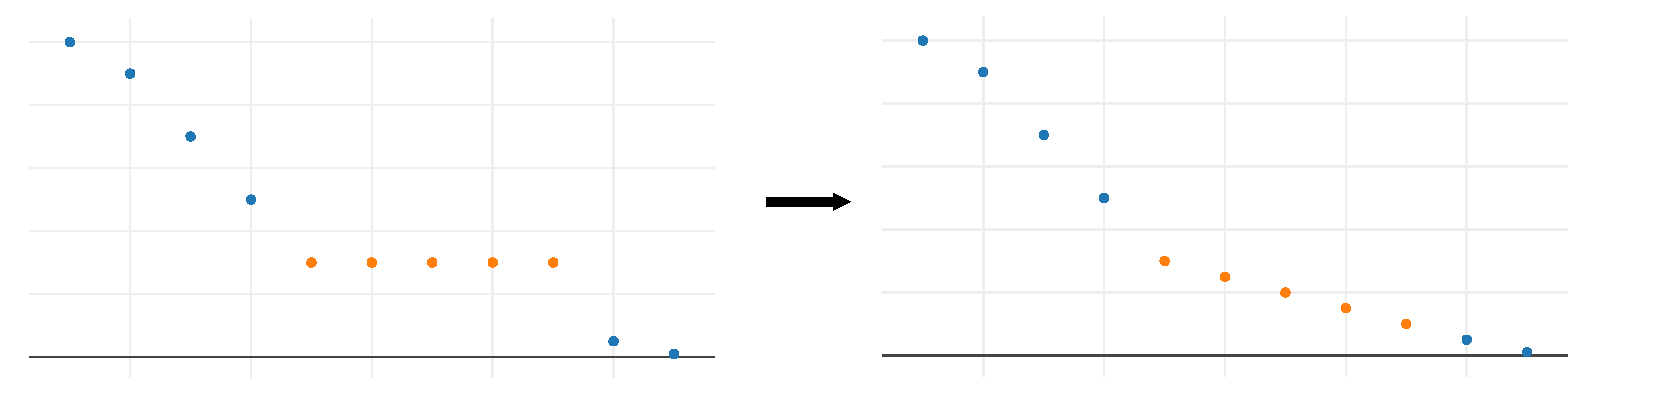
\includegraphics[width=1.0\linewidth]{img/content/chapter3/simple_eig_vals.pdf}
    \caption{Intuición de la proposición \ref{prop:val_prop_sim}. A la izquierda, en naranjo, los valores propios del operador que tienen multiplicidad mayor a $1$ y a la izquierda, en naranjo también, cómo se acomodan entre dos valores propios.}
    \label{fig:simple_eig_vals}
\end{figure}

\begin{proof}
    Dado que $\H_\X$ es un espacio de Hilbert separable y $A$ es compacto y autoadjunto, el teorema espectral \cite{Brezis2011FunctionalEquations} garantiza que $A$ posee un espectro discreto de valores propios $\{ \lambda_j \}_j$, todos positivos y decrecientes hacia $0$, con funciones propias $\{ v_j \}_j$ que constituyen una base ortonormal de $\H_\X$.

    Se definen los operadores $T_k : \H_\X \to \H_\X$ de rango $1$ como
    \[
    T_k \psi = \langle v_k, \psi \rangle v_k, \quad \psi \in \H_\X,
    \]
    los cuales son lineales y continuos. Además, satisfacen
    \[
    T_k v_\ell = \langle v_k, v_\ell \rangle v_k = \delta_{k \ell} v_k,
    \]
    donde $\delta_{k \ell}$ es la delta de Kronecker, ya que $\{ v_j \}_j$ constituye una base ortonormal.

    Sea $\varepsilon \in (0, \lambda_{m+j} - \lambda_{m+j+1})$, se define
    \[
    \varepsilon_k = \frac{\varepsilon (k-j)}{m^2 \cdot j^2}, \quad k \in \{ j, \dots , m+j \},
    \]
    que cumple $\varepsilon_k < \varepsilon < \lambda_{m+j} - \lambda_{m+j+1}$. A partir de esto, se define 
    \[
    B^\varepsilon = \sum_{k=j}^{m+j} \varepsilon_k T_k,
    \]
    el cual, al ser una suma de $m$ operadores de rango $1$ con rangos ortogonales, tiene rango $m$.

    Para \( v_\ell \) con $\ell \notin \{ j, \dots, m+j \}$, se verifica
    \[
    (C_X + B^\varepsilon) v_\ell = C_X v_\ell + B^\varepsilon v_\ell = C_X v_\ell = \lambda_\ell v_\ell.
    \]
    Es decir, $C_X + B^\varepsilon$ conserva los mismos valores propios y funciones propias de $C_X$ para $\ell \notin \{ j, \dots, m+j \}$. En cambio, para $\ell \in \{ j, \dots, m+j \}$ se tiene
    \[
    (C_X + B^\varepsilon) v_\ell = C_X v_\ell + B^\varepsilon v_\ell = \lambda_\ell v_\ell + \sum_{k=j}^{m+j} \varepsilon_k T_k v_\ell = \lambda_\ell v_\ell + \sum_{k=j}^{m+j} \varepsilon_k \delta_{k \ell} v_k = \lambda_\ell v_\ell + \varepsilon_\ell v_\ell.
    \]
    Por lo tanto,
    \[
    (C_X + B^\varepsilon)v_\ell = (\lambda_\ell + \varepsilon_\ell) v_\ell,
    \]
    lo que implica que $\Tilde{\lambda}_\ell = \lambda_\ell + \varepsilon_\ell$ es un valor propio de $C_X + B^\varepsilon$ con función propia $v_\ell$. Estos valores propios son simples ya que
    \[
    \lambda_{j-1} < \lambda_j = \lambda_j + \frac{\varepsilon (j-j)}{m^2 j^2} = \Tilde{\lambda}_j < \Tilde{\lambda}_{m+j} = \lambda_{m+j} + \frac{\varepsilon m}{m^2 j^2} < \lambda_{m+j+1}.
    \]

    En consecuencia, $C_X + B^\varepsilon$ tiene los primeros $N$ valores propios simples con las mismas funciones propias. Finalmente, para $\psi \in \H_\X$, se cumple
    \[
    \| B^\varepsilon \psi \| \leq \sum_{k=j}^{m+j} \varepsilon_k \| T_k \psi \| = \sum_{k=j}^{m+j} \varepsilon_k | \langle v_k, \psi \rangle | \| v_k \| \leq \sum_{k=j}^{m+j} \varepsilon_k \| v_k \| \| \psi \| = \sum_{k=j}^{m+j} \varepsilon_k \| \psi \|,
    \]
    con lo que
    \[
    \| B^\varepsilon \| \leq \sum_{k=j}^{m+j} \varepsilon_k  = \sum_{k=j}^{m+j} \frac{\varepsilon (k-j)}{m^2 j^2} \leq \varepsilon \sum_{k=j}^{m+j} \frac{1}{m j^2} = \frac{\varepsilon}{j^2} \leq \varepsilon \sum_{j \geq 1} \frac{1}{j^2} = C \cdot \varepsilon.
    \]

    Cabe señalar que este factor $1/j^2$ no es estrictamente necesario para una única ventana de valores propios no simples, aunque facilita la extensión de la demostración a una cantidad infinita de ventanas con dicha característica.
\end{proof}

\begin{lema}
    $C_X$ es un operador compacto y autoadjunto.
\end{lema}

\begin{proof}
    Ya se estableció previamente, en el corolario \ref{cor:CX_autoad}, que $C_X$ es autoadjunto, por lo que únicamente resta demostrar su compacidad. Sea $\{ \psi_n \}_n \subset \H_\X$ una sucesión débilmente convergente a $\psi$, es decir, para toda $\phi \in \H_\X$ y $\varepsilon > 0$, existe un $n_0 \in \N$ tal que, para $n \geq n_0$, se cumple
    \[
    \langle \psi_n - \psi, \phi \rangle \to 0.
    \]
    Se debe probar que $C_X \psi_n$ converge en norma a $C_X \psi$. Para ello, se tiene:
    \[
    \begin{aligned}
        \| C_X (\psi_n - \psi) \| & \leq \int_\X | \psi_n (x) - \psi (x) | \| \Phi_\X (x) \| d \mu_\X (x) \\
        & = \int_\X | \langle \psi_n - \psi, \Phi_\X (x) \rangle | \| \Phi_\X (x) \| d \mu_\X (x) \\
        & \leq \left ( \int_\X | \langle \psi_n - \psi, \Phi_\X (x) \rangle |^2 d \mu_\X (x) \right )^{1/2} \left ( \int_\X \| \Phi_\X (x) \|^2 d \mu_\X (x) \right )^{1/2} \\
        & = \left ( \int_\X | \langle \psi_n - \psi, \Phi_\X (x) \rangle |^2 d \mu_\X (x) \right )^{1/2} \left ( \int_\X k(x,x)^2 d \mu_\X (x) \right )^{1/2} \\
        & \to 0,
    \end{aligned}
    \]
    donde se ha aplicado la propiedad reproductora para establecer que
    \[
    \psi_n (x) - \psi (x) = \langle \psi_n - \psi, \Phi_\X (x) \rangle,
    \]
    y la desigualdad de Hölder para separar en dos integrales.
\end{proof}

\begin{teo}
    Sea $\delta \in (0, 1)$, si $\U \H_X \subset \H_X$, $\G \R^p \subset \H_X$, $\B \R^n \subset \H_X$, $\H_\X$ es equivalente en norma a $H^{\nu + n/2}$ y 
    \[
    8\|k\|^2_\infty \ln(2/\delta) \leq \frac{1}{2} (N+1)^{-5/2},
    \]
    entonces con probabilidad al menos $(1-\delta)^4$ se tiene que
     \begin{equation*}
        \| \U - \U_N \|_{\H_{\X, N} \to L^2(\X; \mu_\X)} \leq C N^{-1/2}.
    \end{equation*}
    \begin{equation*}
    \| \G - \G_N \|_{\R^p \to L^2(\X; \mu_\X)} \leq C N^{-1/2}
    \end{equation*}
    \begin{equation*}
    \| \B - \B_N \|_{\R^n \to L^2(\X; \mu_\X)} \leq C N^{-1/2}
    \end{equation*}
    con $C$ alguna constante que no depende ni de $N$ ni de $\delta$.
\end{teo}

\begin{proof}
    Ahora se elimina la hipótesis de la simplicidad de los valores propios de $C_X$, que es compacto y autoadjunto. Si se supone que existe un valor propio con multiplicidad mayor que $1$, entonces por la proposición \ref{prop:val_prop_sim}, se tiene que existe $B^\varepsilon$ de rango finito que cumple que $C_X + B^\varepsilon$ tiene los primeros $N+1$ valores propios simples, con las mismas funciones propias y $\| B^\varepsilon \| \leq C \varepsilon$. 

    Se define un nuevo aproximante de Koopman como
    \[
    \U^\varepsilon = (C_X + B^\varepsilon)^{-1} C_{XX^+}
    \]
    y su aproximante en dimensión finita respectivo es
    \[
    \U^\varepsilon_N = (C_X^N + B^\varepsilon)^{-1} C_{XX^+}^N
    \]
    donde $B^\varepsilon$ se deja sin cambios ya que es de rango finito. Estos operadores cumplen, para $\psi \in \H_\X$, que
    \[
    \begin{aligned}
        \| \U\psi - \U^\varepsilon\psi \| & = \| C_X^{-1} C_{XX^+} \psi - (C_X + B^\varepsilon)^{-1} C_{XX^+} \psi \| \\
        & = \| C_X^{-1} \Tilde{\psi} - (C_X + B^\varepsilon)^{-1} \Tilde{\psi} \| \\
        & = \| \hat{\psi} - \hat{\psi}_\varepsilon \|
    \end{aligned} 
    \]
    en donde
    \[
    C_{XX^+}\psi = \Tilde{\psi}, \quad C_X \hat{\psi} =  \Tilde{\psi}, \quad (C_X + B^\varepsilon)\hat{\psi}_\varepsilon = \Tilde{\psi}.
    \]
    Así
    \[
    C_X \hat{\psi} = (C_X + B^\varepsilon)\hat{\psi}_\varepsilon,
    \]
    con lo que
    \[
    C_X (\hat{\psi} - \hat{\psi}_\varepsilon) = B^\varepsilon \hat{\psi}_\varepsilon
    \]
    y así
    \[
    \|C_X (\hat{\psi} - \hat{\psi}_\varepsilon)\| = \|B^\varepsilon \hat{\psi}_\varepsilon\|.
    \]

    Gracias a la inyectividad de $C_X$, existe una constante $c_1$ tal que 
    \[
    \| \hat{\psi} - \hat{\psi}_\varepsilon \| \leq \frac{1}{c_1} \| C_X (\hat{\psi} - \hat{\psi}_\varepsilon) \| \leq \| B^\varepsilon \| \| \hat{\psi}_\varepsilon \| \leq C \cdot \varepsilon \| \hat{\psi}_\varepsilon \|. 
    \]
    Con ello notar que
    \[
    C_X \hat{\psi}_\varepsilon  = -B^\varepsilon \hat{\psi}_\varepsilon  + (B^\varepsilon + C_X)\hat{\psi}_\varepsilon
    \]
    así
    \[
    \| C_X \hat{\psi}_\varepsilon \| \leq \| B^\varepsilon \hat{\psi}_\varepsilon \| + \| (B^\varepsilon + C_X)\hat{\psi}_\varepsilon\| \leq C \cdot \varepsilon  \| \hat{\psi}_\varepsilon \| + \| (B^\varepsilon + C_X)\hat{\psi}_\varepsilon\|. 
    \]
    
    Utilizando la inyectividad de $C_X$
    \[
    c_1 \|\hat{\psi}_\varepsilon\| \leq \| C_X \hat{\psi}_\varepsilon \| \leq  C \cdot \varepsilon  \| \hat{\psi}_\varepsilon \| + \| (B^\varepsilon + C_X)\hat{\psi}_\varepsilon\|
    \]
    con ello
    \[
    (c_1 - C\varepsilon)  \|\hat{\psi}_\varepsilon\| \leq \| (B^\varepsilon + C_X)\hat{\psi}_\varepsilon\| = \| \Tilde{\psi} \|
    \]
    
    Tomando $\varepsilon$ tal que $c_1 - C \varepsilon > 0$ se tiene que
    \[
    \|\hat{\psi}_\varepsilon\| \leq \frac{1}{c_1 - C\varepsilon} \| \Tilde{\psi} \| = \frac{1}{c_1 - C\varepsilon} \| C_{XX^+} \psi \| \leq \frac{1}{c_1 - C\varepsilon} \| C_{XX^+} \| \| \psi \|
    \]

     Y así
    \[
     \| \U\psi - \U^\varepsilon\psi \| = \| \hat{\psi} - \hat{\psi}_\varepsilon \| \leq \frac{C \cdot \varepsilon}{c_1 - C \cdot \varepsilon} \| C_{XX^+} \| \| \psi \| \leq \frac{C \cdot \varepsilon}{c_1} \| C_{XX^+} \| \| \psi \| = c_2 \| \psi \|.
    \]

    De manera análoga, existe una constante $c_3$ tal que 

    \[
    \| \U^\varepsilon_N - \U_N \| \leq c_3 \cdot \varepsilon.
    \]
    
    Luego, al igual que antes se tiene
    \[
    \begin{aligned}
        \| \U - \U_N \| & \leq \| \U - \U^\varepsilon \| + \| \U^\varepsilon - \U_N^\varepsilon \| + \| \U_N^\varepsilon - \U_N \| \\
        & \leq c_2 \cdot \varepsilon + C N^{-1/2} + c_3 \cdot \varepsilon.
    \end{aligned}
    \]

   Tomando $\varepsilon = c_4 N^{-1/2}$, con $c_4 = c_1/(2C)$ que cumple
   \[
   C  \varepsilon = C c_4 N^{-1/2} \leq C c_4 = c_1/2 < c_1
   \]
   con lo que se cumple la condición $c_1 - C  \varepsilon > 0$, se tiene
   \[
   \| \U - \U_N \| \leq c_5 N^{-1/2}.
   \]
\end{proof}

\section{Resultados numéricos}

A pesar de que las cotas de error del \textit{kernel} Extended Dynamic Mode Decomposition serán útiles para la construcción de la cota de error para el filtro, también son interesantes por sí solas y se puede visualizar al aproximar distintos sistemas dinámicos y operadores de manera empírica.
Será de interés en esta sección no solo explorar cómo un sistema lineal puede aproximar otro sistema de interés mediante el \textit{sampleo} de datos, sino también el orden de decaimiento del error cometido en función del número de puntos \textit{sampleados} $N$.

\subsection{kEDMD para el caso lineal}

Un primer caso de interés es estudiar qué ocurre cuando se tiene un sistema lineal, esto es considerar un sistema de la forma
\begin{equation*}
    \mathbf{x}_{k+1} = \mathbf{A} \mathbf{x}_{k}.
\end{equation*}
Para este ejemplo se considera
\begin{equation*}
    \mathbf{A} = 
    \begin{pmatrix}
        1.01 & 0.04 & 0 \\
        0.01 & 1.02 & \alpha \\
        0 & 0.04 & 1.02
    \end{pmatrix}
\end{equation*}
en donde el parámetro $\alpha$ determinará el comportamiento del sistema dinámico en el tiempo. Se considera como distribución de probabilidad en $\X = \R^n$ una normal $N(0_{3}, 3 \cdot I_{3\times3})$, para la dinámica se considera un ruido normal $N(0_{3}, 10^{-7} \cdot I_{3\times3})$ y $\mathbf{x}_0 = (0.1, 0.1, 0.1)^T$ como condición inicial. Notar que en este ejemplo no se satisface la hipótesis de compacidad, pero el sistema con alta probabilidad se mantiene en un compacto en horizonte de tiempo finito.

Se compara la dinámica original con aquella linealizada vía Operador de Koopman \textit{sampleando} 2500 puntos del espacio de estados, utilizando \textit{kernel} de Matérn de parámetro $\nu = 1/2$ y un ancho de banda $\gamma = 10^{-3}$. Esto es, se compara con el sistema
\begin{align*}
    \mathbf{z}_{k+1} = & \mathbf{U}_N \mathbf{z}_k \\
    \hat{\mathbf{x}}_k = & \mathbf{B}_N \mathbf{z}_k \\
    \mathbf{z}_0 = & \Phi_N(\mathbf{x}_0)
\end{align*}

Se compara lo obtenido para $\alpha \in \{ -0.3, -0.1, 0.05\}$.
\begin{figure}[htbp]
    \centering
    \begin{subfigure}[b]{0.32\textwidth}
        \centering
        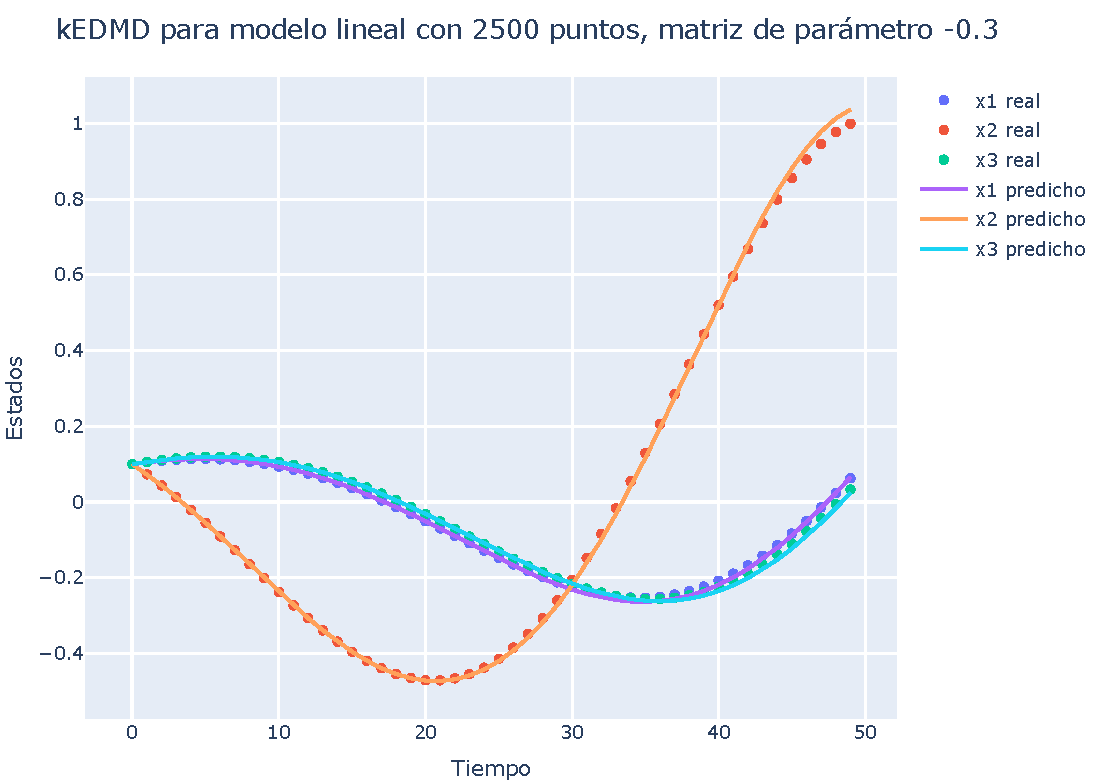
\includegraphics[width=\textwidth]{img/content/chapter3/Linear1.pdf}
        \caption{$\alpha=-0.3$}
        \label{fig:Linear1}
    \end{subfigure}
    \hfill
    \begin{subfigure}[b]{0.32\textwidth}
        \centering
        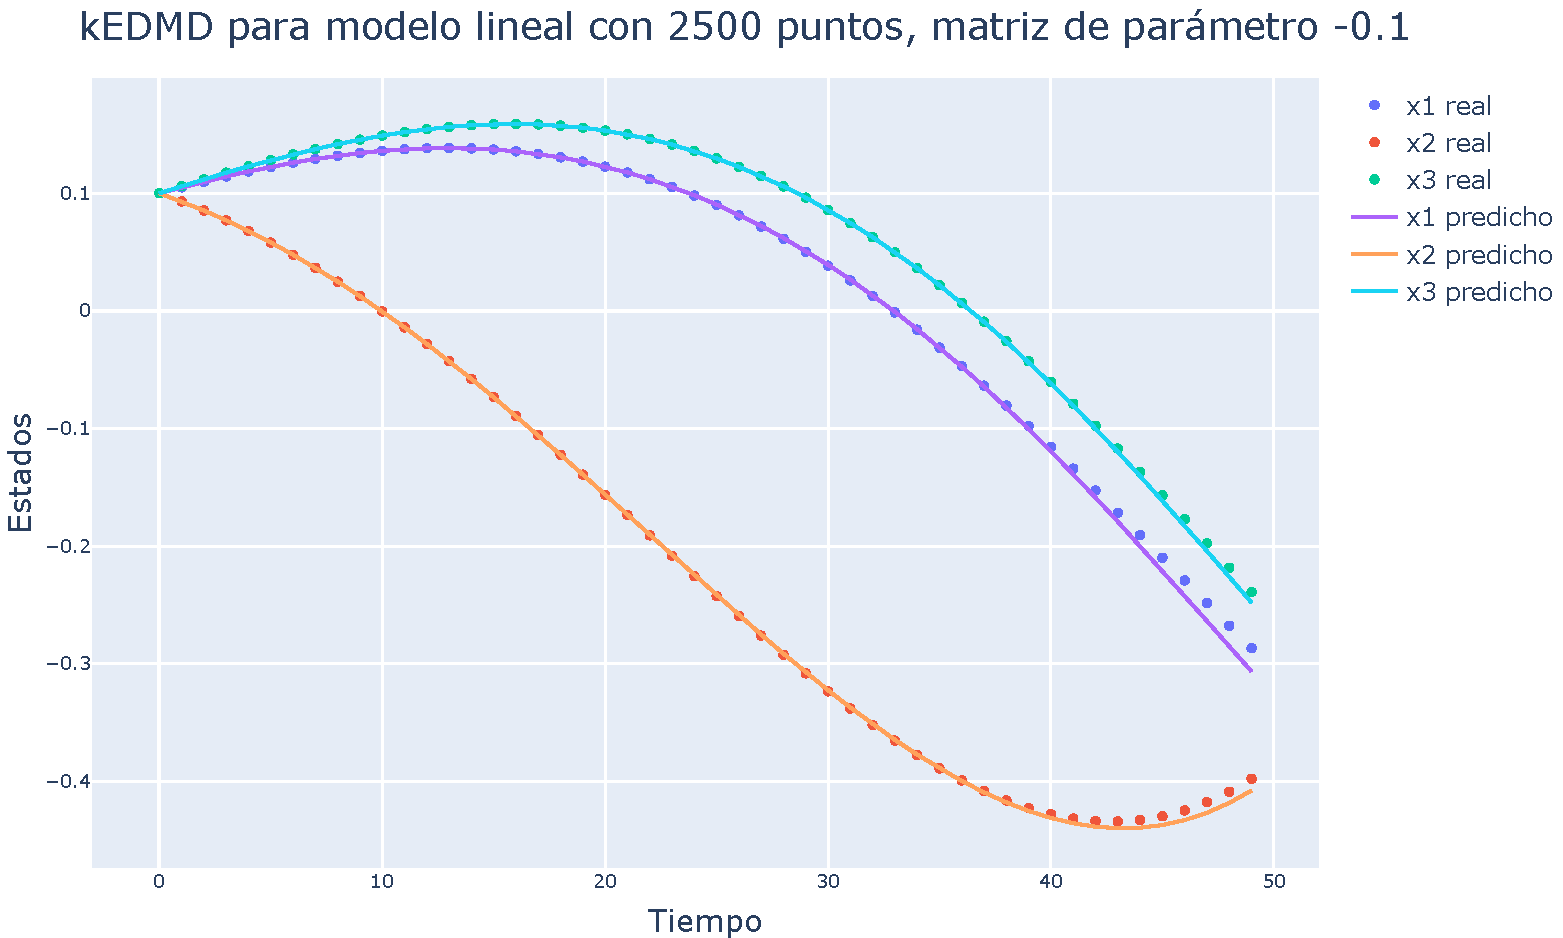
\includegraphics[width=\textwidth]{img/content/chapter3/Linear2.pdf}
        \caption{$\alpha=-0.1$}
        \label{fig:Linear2}
    \end{subfigure}
    \hfill
    \begin{subfigure}[b]{0.32\textwidth}
        \centering
        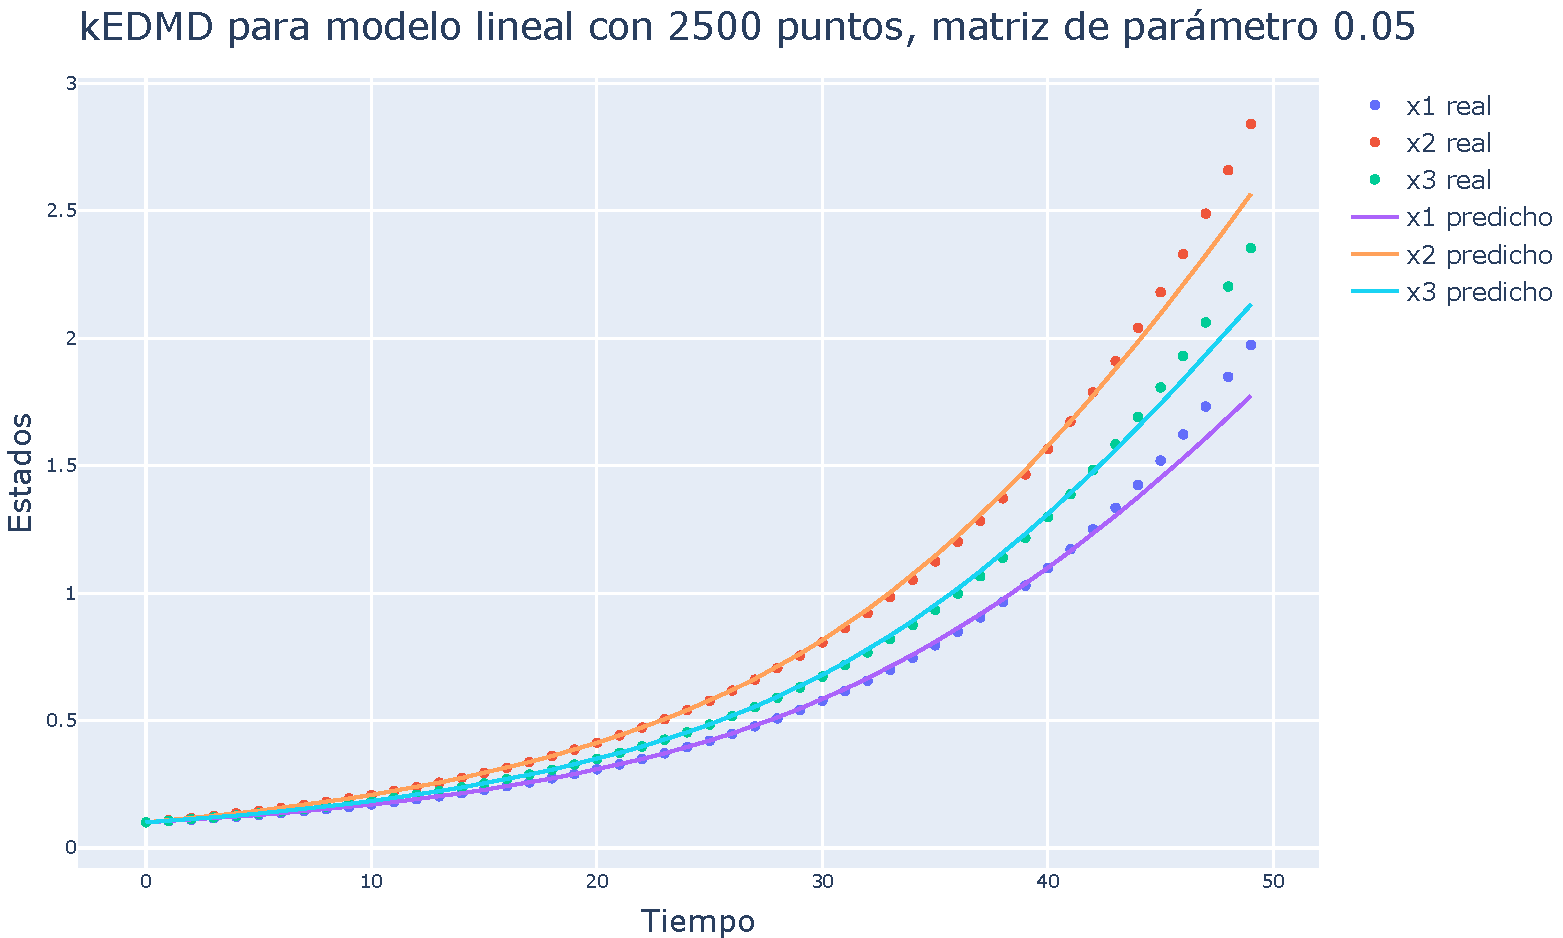
\includegraphics[width=\textwidth]{img/content/chapter3/Linear3.pdf}
        \caption{$\alpha=0.05$}
    \end{subfigure}
    \caption{Ilustración de los tres casos de $\alpha$ elegidos para la comparación entre el sistema lineal original y el sistema linealizado por Koopman a 2500 puntos \textit{sampleados} de una variable aleatoria normal. En forma de puntos se dejan los valores reales que toma el sistema y en línea continua los valores entregados por el sistema linealizado, que se consideran como predicción.}
    \label{fig:Comp_traj_lin}
\end{figure}
Aunque la cota en \eqref{eq:kEDMD_bound} no hace referencia directa a la diferencia en norma de las trayectorias, es de interés analizar el orden en que decae el error en función de $N$, para ello se calcula la diferencia en norma de las trayectorias generadas para $N \in \{ 100k : k \in \{1, \dots, 30\} \}$. 

En la figura \ref{fig:Comp_traj_lin} se observa que las trayectorias obtenidas con el sistema linealizado vía Koopman son muy cercanas a las obtenidas con el sistema lineal original, solo difiriendo en zonas donde el sistema original toma valores muy altos, lo que se puede asociar a la poca probabilidad de \textit{sampleo} que le da la distribución normal elegida a puntos muy alejados del origen. \\
Mientras que en la figura \ref{fig:ErrorLin} se observa que en realidad el orden de decaimiento del error en función de $N$ es mayor que $N^{-1/2}$, mejorando la cota mostrada en \eqref{eq:kEDMD_bound}.
\begin{figure}[h]
    \centering
    \begin{subfigure}[b]{0.32\textwidth}
        \centering
        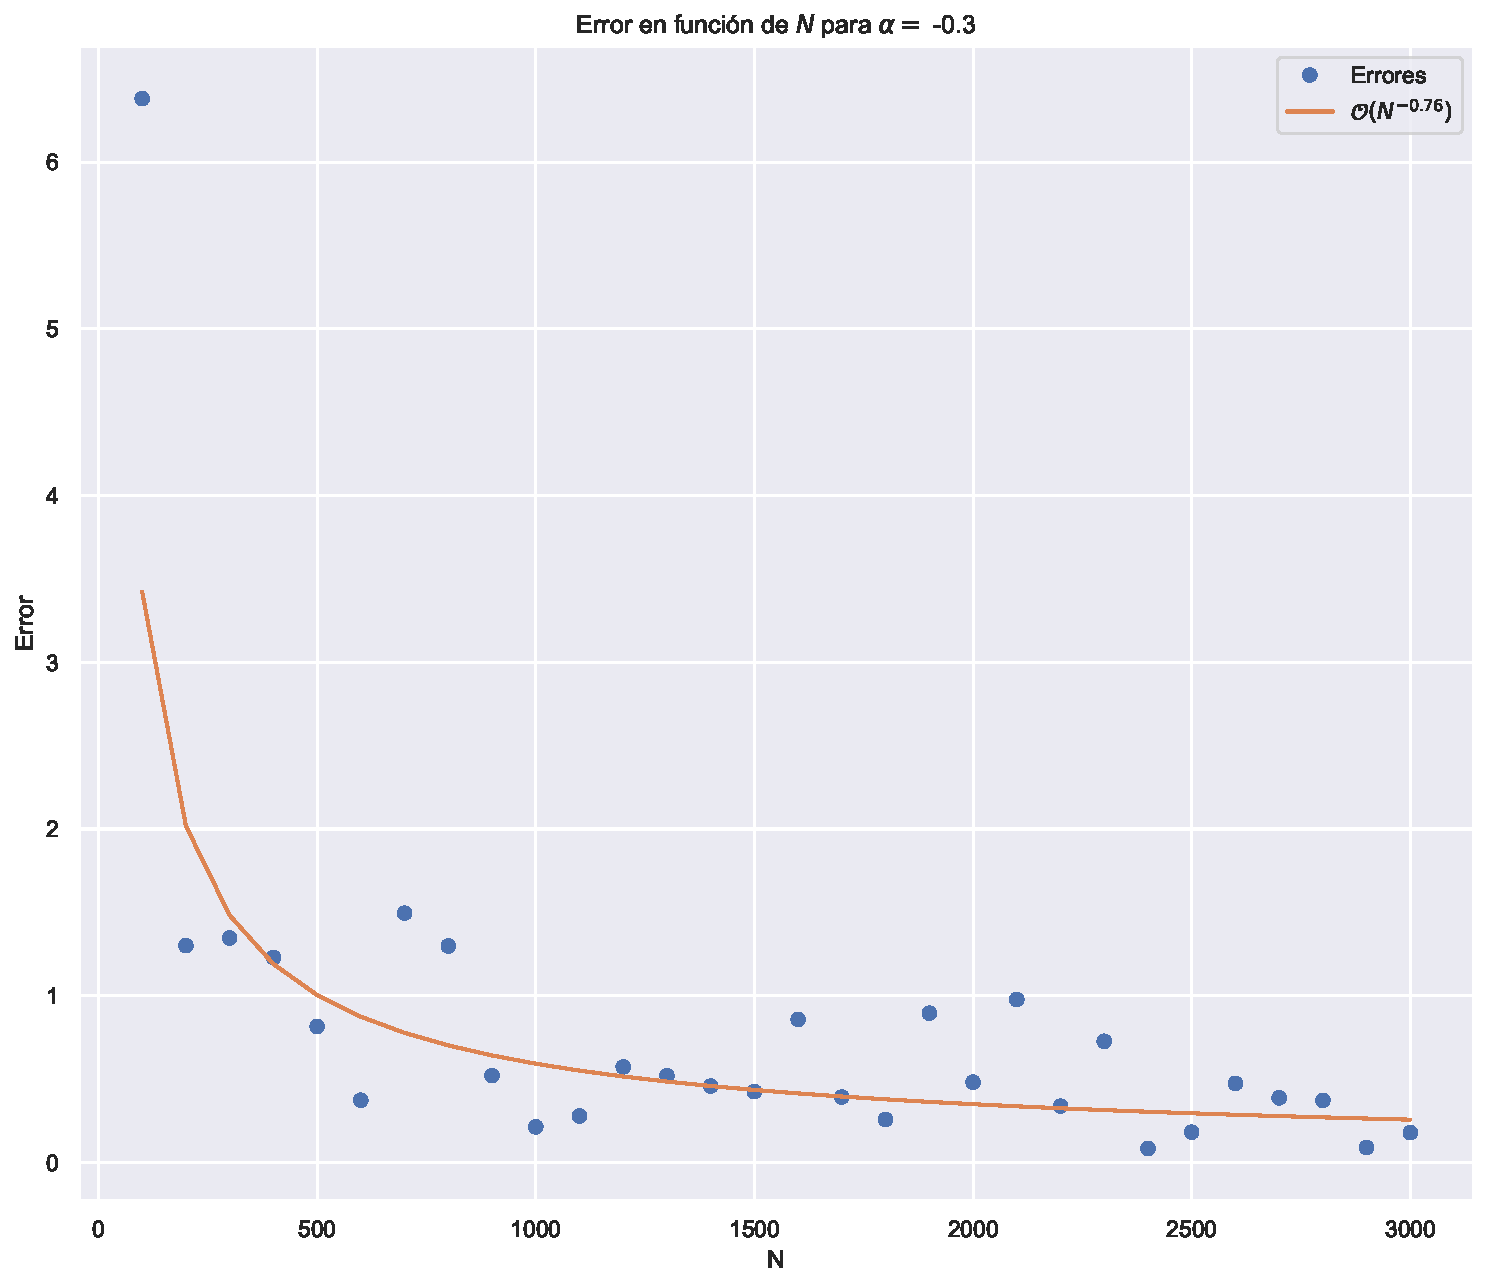
\includegraphics[width=\textwidth]{img/content/chapter3/Linear1Errors.pdf}
        \caption{$\alpha=-0.3$}
        \label{fig:Linear1Errors}
    \end{subfigure}
    \hfill
    \begin{subfigure}[b]{0.32\textwidth}
        \centering
        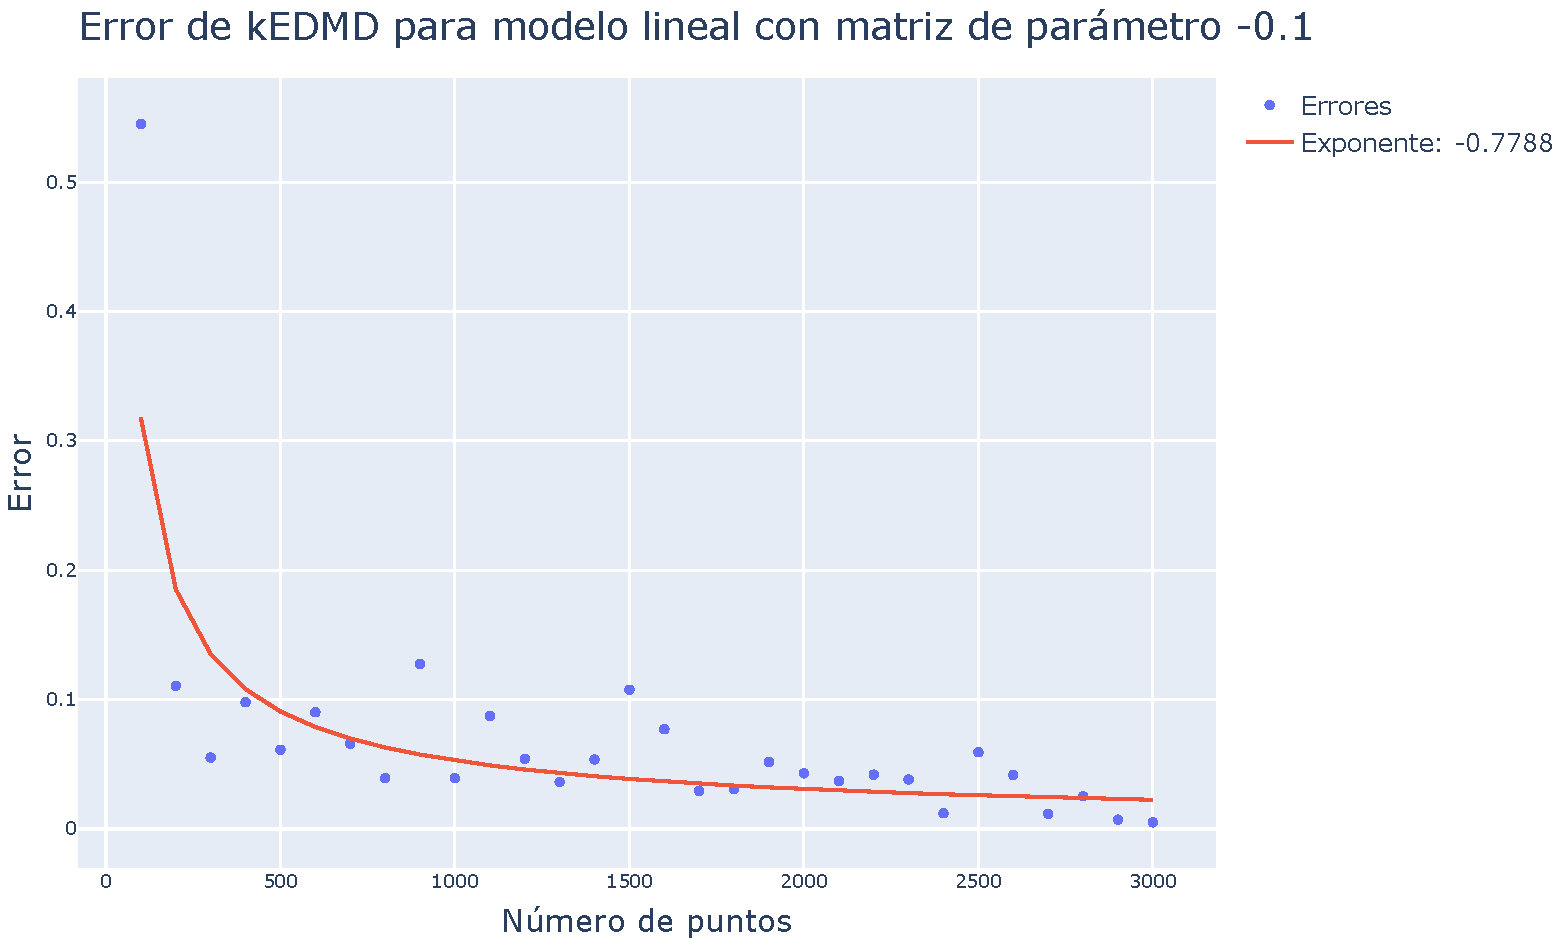
\includegraphics[width=\textwidth]{img/content/chapter3/Linear2Errors.pdf}
        \caption{$\alpha=-0.1$}
        \label{fig:Linear2Errors}
    \end{subfigure}
    \hfill
    \begin{subfigure}[b]{0.32\textwidth}
        \centering
        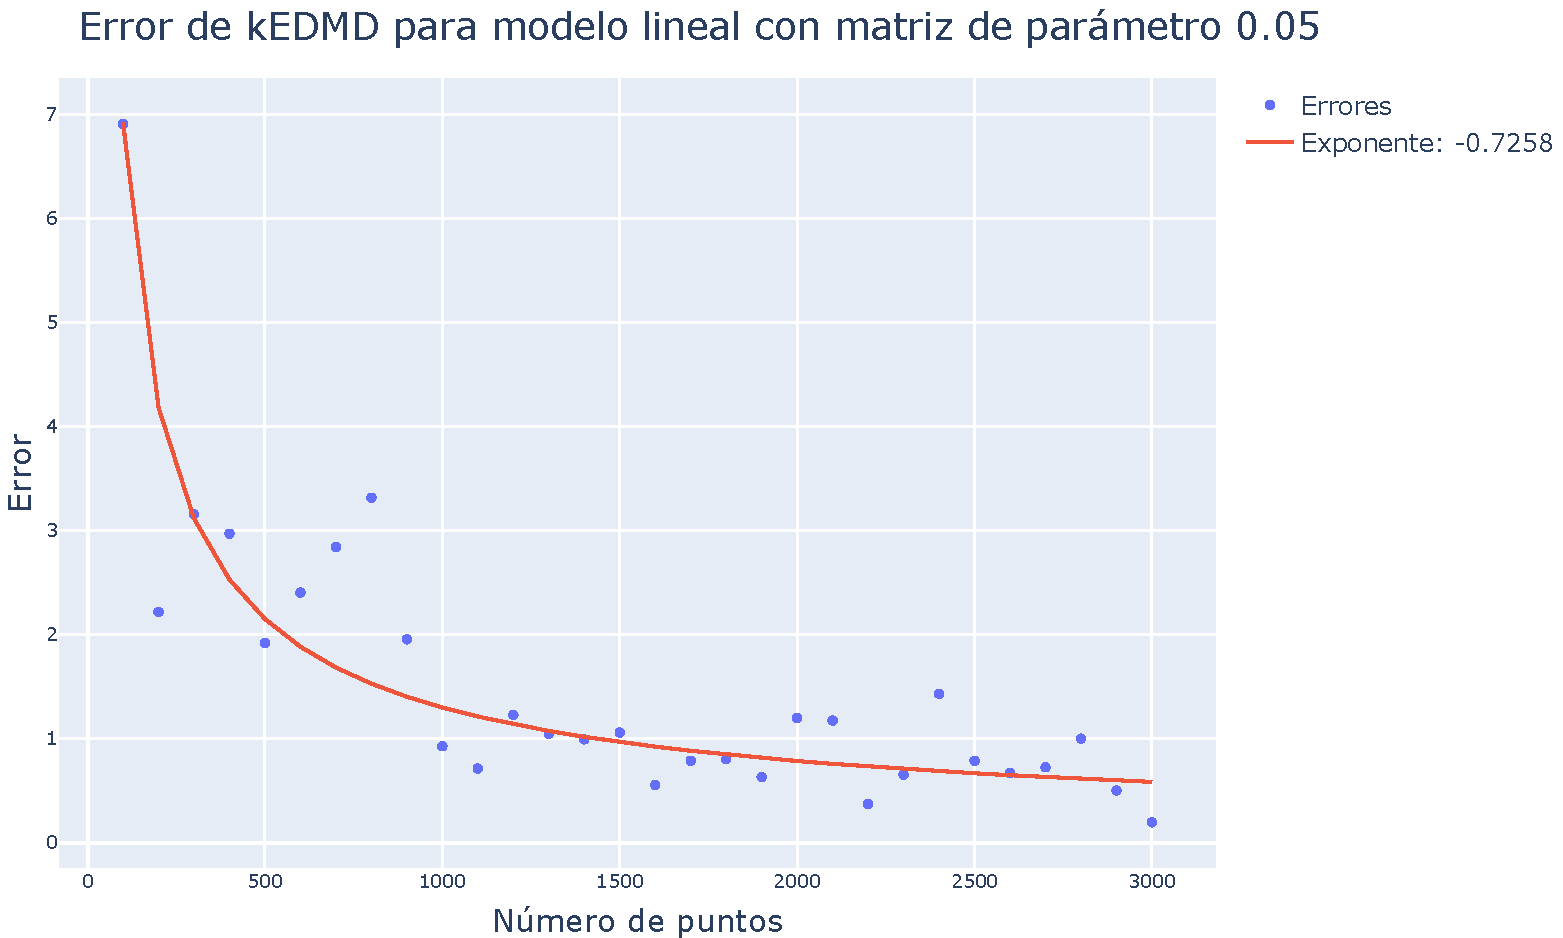
\includegraphics[width=\textwidth]{img/content/chapter3/Linear3Errors.pdf}
        \caption{$\alpha=0.05$}
        \label{fig:image3}
    \end{subfigure}
    \caption{Ilustración de los tres casos de $\alpha$ elegidos para la evolución en función de $N$ de la diferencia en norma entre el sistema lineal original y el sistema linealizado por Koopman a $N$ puntos \textit{sampleados} de una variable aleatoria normal. En forma de puntos se deja la evolución observada del error y en línea continua la mejor curva de la forma $C \cdot N^{a}$, donde $a$ es el exponente que se deja en la leyenda.}
    \label{fig:ErrorLin}
\end{figure}
\subsection{kEDMD para modelos utilizados en epidemiología}
Para esta sección se ilustrarán los resultados de kEDMD para modelos epidemiológicos de tipo SIR y SIRS. Se supondrá que la población está normalizada, esto es, que cada estado está en $[0, 1]$.\\
Dado que no se consideran nacimientos ni muertes, se puede decir que el espacio de estados de este modelo es, sin considerar los eventuales factores estocásticos, un $(n-1)$-simplex, siendo $n$ la cantidad de compartimentos considerados, que se define como el conjunto
\begin{equation*}
    \Delta_{n-1} = \left \{ x \in \R^n : \sum_{i=1}^n x_i = 1, \, x_i \geq 0, \, \forall i \in \{1, \dots, n\} \right \}.
\end{equation*}
De este conjunto se puede \textit{samplear} de manera eficiente desde una distribución Dirichlet \cite{Frigyik2010IntroductionProcesses}, y se encuentra implementado en las principales librerías con funcionalidades estadísticas como SciPy \cite{Virtanen2020SciPyPython}, que será la utilizada en este trabajo.\\
La densidad de una variable aleatoria Dirichlet con parámetros $\alpha_1, \alpha_2, \ldots, \alpha_K$ se define como:
\[
f(x_1, x_2, \ldots, x_K; \alpha_1, \alpha_2, \ldots, \alpha_K) = \frac{1}{B(\alpha)} \prod_{i=1}^{K} x_i^{\alpha_i - 1}
\]
donde $x_i \geq 0$ para todo $i$, $\sum_{i=1}^{K} x_i = 1$, y
\[
B(\alpha) = \frac{\prod_{i=1}^{K} \Gamma(\alpha_i)}{\Gamma\left(\sum_{i=1}^{K} \alpha_i\right)}
\]
es la función beta multivariable, y $\Gamma(\cdot)$ es la función gamma. En la figura \ref{fig:Dirichlet_samples} se puede apreciar la diferencia de \textit{samplear} para diferentes valores de $\alpha$. Un valor de $\alpha$ con entradas iguales genera la misma dispersión en todas las direcciones, siendo $(1, 1, 1)$ la variable aleatoria uniforme en $\Delta_{n-1}$, mientras que valores altos de $\alpha$ generan una alta concentración de muestras en el centro del conjunto. Por otro lado valores desiguales generar mayor cantidad de muestras en alguna de las caras del conjunto.
\begin{figure}[htbp]
    \centering
    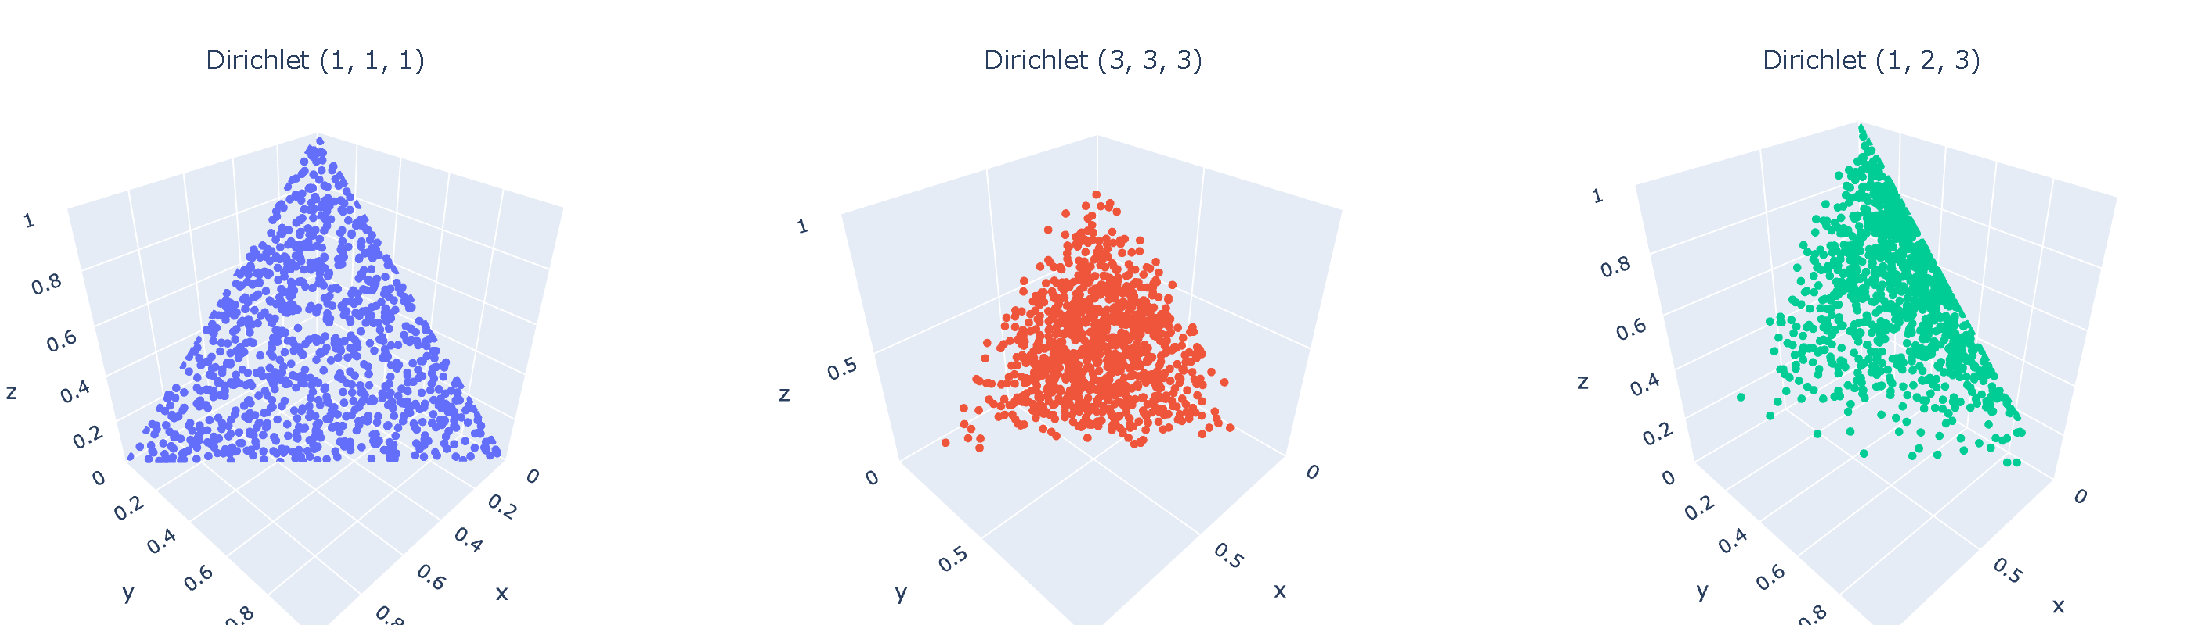
\includegraphics[width=0.95\linewidth]{img/content/chapter3/Dirichlet.pdf}
    \caption{1000 muestras de una variable aleatoria Dirichlet para diferentes valores de $\alpha$, observando dos casos de $\alpha$ con valores homogéneos y uno con valores heterogéneos, lo que provoca un desbalance de muestras.}
    \label{fig:Dirichlet_samples}
\end{figure}

Se visualizará la aproximación por kEDMD para los modelos SIR y SIRS, con la misma configuración en común, salvo, obviamente, el parámetro $\alpha$ correspondiente al segundo modelo. Se utilizó \textit{kernel} de Matérn de parámetro $\nu=1/2$ y ancho de banda $\gamma=10^{-3}$. Se utiliza una distribución Dirichlet de parámetro $(1,1,1)$ como variable aleatoria asociada al espacio de estados y ruido aditivo centrado y Gaussiano de matriz de covarianza $10^{-7} I_{3 \times 3}$, de estas distribuciones se \textit{samplearán} $N=1000$ puntos. Se toma como condición inicial $\mathbf{x}_0 = (0.9, 0.1, 0.0)$ y los resultados obtenidos se pueden ver en las figuras \ref{fig:Comp_traj_SIR} y \ref{fig:Comp_traj_SIRS}. 

Similar a lo hecho en el caso lineal, en las figuras \ref{fig:ErrorSIR} y \ref{fig:ErrorSIRS} se comparan las diferencias en norma entre las trayectorias originales y las trayectoria linealizadas, con la mejor curva de la forma $C \cdot N^{a}$, para observar si los errores andan en el orden de decaimiento en \eqref{eq:kEDMD_bound}.

Se observa nuevamente que la discrepancia entre las trayectorias en efecto anda del orden de la cota expuesta en este capítulo, incluso con decaimientos aún más rápidos.

Se comparan las trayectorias generadas por el sistema original con las generadas por kEDMD, utilizando exactamente la misma configuración del sistema anterior, solo cambiando la dinámica.

Nuevamente se observa que el orden de discrepancia de las trayectorias es de un orden similar, o incluso menor, al visto en la cota \ref{eq:kEDMD_bound}.

% Capítulo 4: Algoritmo de filtraje en tiempo discreto y estimación de parámetros
\chapter{Algoritmo de filtraje en tiempo discreto}
El hecho de que sea posible construir un sistema lineal que se asemeje significativamente a otro sistema, eventualmente no lineal, sugiere la viabilidad de emplear dicho sistema linealizado para abordar problemas de filtraje no lineal mediante el uso del Filtro de Kalman. 

En la literatura, ya existen diversas conexiones entre el Filtro de Kalman y el operador de Koopman. Por ejemplo, se ha explorado su utilización para la corrección de errores \cite{Jiang2022CorrectingFilters}, la estimación de modos de Koopman \cite{Liu2024EstimateFilter}, y la mejora de algoritmos como el Filtro de Kalman Extendido \cite{Ramadan2024ExtendedControl}. Además, algoritmos similares al que se propone en este capítulo han sido presentados y validados en diferentes aplicaciones, como se observa en \cite{Wang2022KoopmanSystem, Wang2023Innovation-saturatedOutliers, Netto2018RobustEstimation, Syed2021Koopman-basedXFEL, HuangData-DrivenFlight, Yang2025Data-DrivenPredictor}. 

Por otra parte, trabajos pioneros en la línea de observabilidad e identificación de sistemas, liderados por Surana y colaboradores, han proporcionado una base sólida en este campo, como se documenta en \cite{Surana2016KoopmanSystems, Surana2016LinearFramework}.

Por otro lado, hay enfoques que aplican la \textit{kernel Bayes Rule} a sistemas dinámicos y filtraje, donde se incluyen los trabajos de Song, Fukumizu y colaboradores \cite{Fukumizu2004DimensionalitySpaces, Fukumizu2013KernelKernels, Fukumizu2015NonparametricEmbedding, Song2009HilbertSystems, Song2013KernelModels}, lo que aparece de manera natural al demostrar la utilidad de los operadores para representar esperanzas condicionales.

Aunque el algoritmo propuesto en este capítulo no constituye una contribución original en términos de su estructura, sí lo es la justificación de su funcionamiento y convergencia bajo el supuesto de contar con un muestreo suficiente de puntos. En este contexto, se demuestra, en base a las cotas probadas anteriormente para la aproximación vía \textit{kernel} Dynamic Mode Decomposition, que un filtro subóptimo representado en dimensión finita converge al óptimo en dimensión infinita. 

El objetivo principal de este capítulo es demostrar que, bajo ciertas hipótesis, la tasa de convergencia del algoritmo es del orden de $N^{-1/2}$, lo que lo posiciona como un competidor viable frente a otros algoritmos de filtraje presentes en la literatura, tales como los filtros de partículas, discutidos previamente en la sección de preliminares.

Para ello, se propone primero descomponer el error del Filtro de Kalman aplicado a dos sistemas lineales, formulando este error en función de los datos provenientes de los sistemas. Este análisis, hasta la fecha de redacción de este trabajo, no se encuentra documentado en la literatura y, por lo tanto, constituye una contribución original de esta investigación.

Posteriormente, se construye el filtro propuesto, denominado \textit{Koopman Kalman Filter} (KKF), siguiendo una metodología análoga a la empleada en el Filtro de Kalman para sistemas lineales con mínimos cuadrados recursivos \cite{Kalman1960AProblems, Triantafyllopoulos2021BayesianBeyond}, y particularmente a como se formula en \cite{Gebhard2019} para la construcción de la denominada \textit{kernel Kalman Rule}.

Finalmente, utilizando los resultados obtenidos en el capítulo anterior junto con la descomposición del error, se demuestra la cota de error propuesta. El desempeño del filtro es evaluado en diferentes sistemas mediante una implementación en Python desarrollada específicamente para este trabajo.

Se muestran resultados numéricos del filtro en modelos epidemiológicos, tanto en problemas de filtraje con observaciones parciales como problemas de estimación de parámetros de estos modelos. El trabajo de Catalán Muñoz \cite{CatalanMunoz2022DesarrolloChile} fue una inspiración para este trabajo al aplicar Filtro de Kalman para estimación de parámetros de un modelo epidemiológico relevante para la realidad de Santiago de Chile. Cabe notar que Mezić et al. ya han aplicado técnicas relacionadas con operador de Koopman para modelos epidemiológicos \cite{Mezic2024ACases}, aunque nunca se habla de filtraje, dinámicas específicas ni estimación de parámetros. 

\section{Descomposición de error de Kalman}

El objetivo de esta sección es analizar el error que se genera entre dos reglas de Kalman, lo cual permitirá cuantificar la discrepancia entre una regla de Kalman aproximante y otra exacta, ambas definidas formalmente más adelante en esta misma sección. Para ello se asumirá que el horizonte de tiempo $T$ es finito, lo que evita tener que preocuparse por el comportamiento de las constantes para tiempos largos.

Para este propósito, se consideran dos sistemas dinámicos observados en un espacio de Hilbert con espacios de estados $E_x$ y de observaciones $E_y$, descritos por las siguientes ecuaciones:  
\begin{equation*}
	\begin{aligned}
		\mu_{i,k}  &= A_{i,k} \mu_{i,k-1} + \nu_{i,k}, \\
		y_{i,k} &= C_{i,k} \mu_{i,k} + \xi_{i,k},
	\end{aligned}
\end{equation*}
donde $A_{i,k} : E_x \to E_x$ y $C_{i,k}: E_x \to E_y$ son operadores lineales; $\nu_{i,k} \in E_x$ y $\xi_{i,k} \in E_y$ representan variables aleatorias con segundo momento finito y operadores de covarianza $\mathcal{Q}_{i,k}$ y $\mathcal{R}_{i,k}$, respectivamente. Todo esto se considera para $i \in \{1,2\}$ y $k \geq 1$.

Cada uno de estos sistemas tiene asociada una regla de Kalman, la cual está definida por las siguientes expresiones:  
\begin{equation*}
	\begin{aligned}
		\mathcal{P}_{i,k}^- &= A_{i,k}^* \mathcal{P}_{i,k-1}^+ A_{i,k} + \mathcal{Q}_{i,k}, \\
		\S_{i,k} &= C_{i,k} \mathcal{P}_{i,k}^- C_{i,k}^* + \mathcal{R}_{i,k}, \\
		\K_{i,k} &= \mathcal{P}_{i,k}^- C_{i,k} \S_{i,k}^{-1}, \\
		\mathcal{P}_{i,k}^+ &= (I - \K_{i,k} C_{i,k}) \mathcal{P}_{i,k}^-, \\
		\hat{\mu}_{i,k} &= A_{i,k} \hat{\mu}_{i,k-1} + \K_{i,k} (y_{i,k} - C_{i,k} \hat{\mu}_{i,k-1}),
	\end{aligned}
\end{equation*}
con $i \in \{1,2\}$ y $k \geq 1$. Aquí, $\mathcal{P}_{i,k}^-$ y $\mathcal{P}_{i,k}^+$ representan los operadores de covarianza del error a priori y a posteriori, respectivamente, mientras que $\K_{i,k}$ es el operador de ganancia de Kalman, todos ellos definidos en los espacios indicados. Estas reglas se inicializan como sigue:
\begin{equation*}
	\hat{\mu}_{i,0} = \mathbb{E}[\mu_{i,0}], \quad \mathcal{P}_{i,0} = \text{Cov}(\mu_{i,0}).
\end{equation*}

Con estas definiciones, se presenta un resultado clave que ilustra cómo la discrepancia en norma entre las reglas de Kalman puede descomponerse en función de las discrepancias en norma de los elementos asociados, junto con la influencia de las iteraciones previas.


\begin{teo}[Descomposición de error de Kalman]
	Sea $k \geq 1$. Si los operadores $\S_{i,k}$ son invertibles, entonces existen constantes $c_{k,j}^i$ con $j \in \{1, \dots, 7\}$, $i \in \{1, 2\}$, tales que se cumplen las siguientes desigualdades:
	\begin{equation*}
		\begin{aligned}
			\| \hat{\mu}_{1,k} - \hat{\mu}_{2,k} \| \leq & \, c_{1,k}^1 \| A_{1,k} - A_{2,k} \| + c_{2,k}^1 \| C_{1,k} - C_{2,k} \| \\ 
			&+ c_{3,k}^1 \| \mathcal{Q}_{1,k} - \mathcal{Q}_{2,k} \| + c_{4,k}^1 \| \mathcal{R}_{1,k} - \mathcal{R}_{2,k} \| \\
			&+ c_{5,k}^1 \| y_{1,k} - y_{2,k} \| + c_{6,k}^1 \| \hat{\mu}_{1,k-1} - \hat{\mu}_{2,k-1} \| \\
			&+ c_{7,k}^1 \| \mathcal{P}_{1,k-1}^+ - \mathcal{P}_{2,k-1}^+ \|,
		\end{aligned}
	\end{equation*}
	y
	\begin{equation*}
		\begin{aligned}
			\| \mathcal{P}_{1,k}^+ - \mathcal{P}_{2,k}^+ \| \leq & \, c_{1,k}^2 \| A_{1,k} - A_{2,k} \| + c_{2,k}^2 \| C_{1,k} - C_{2,k} \| \\ 
			&+ c_{3,k}^2 \| \mathcal{Q}_{1,k} - \mathcal{Q}_{2,k} \| + c_{4,k}^2 \| \mathcal{R}_{1,k} - \mathcal{R}_{2,k} \| \\
			&+ c_{5,k}^2 \| y_{1,k} - y_{2,k} \| + c_{6,k}^2 \| \hat{\mu}_{1,k-1} - \hat{\mu}_{2,k-1} \| \\
			&+ c_{7,k}^2 \| \mathcal{P}_{1,k-1}^+ - \mathcal{P}_{2,k-1}^+ \|.
		\end{aligned}
	\end{equation*}

	Aquí, las constantes $c_{k,j}^i$ son positivas y dependen de $k$ únicamente a través de las normas $\| A_{i,k} \|$, $\| C_{i,k} \|$, $\| \mathcal{Q}_{i,k} \|$, $\| \mathcal{R}_{i,k} \|$, $\| \S_{i,k}^{-1} \|$, $\| y_{i,k} \|$, $\| \hat{\mu}_{i,k-1} \|$ y $\| \mathcal{P}_{i,k-1}^+ \|$.
	\label{teo:error_kalman}
\end{teo}

\begin{proof}
Se observa que  
\begin{equation*}
	\begin{aligned}
		&	\| \hat \mu_{1,k} - \hat \mu_{2,k} \|_{E_x}  \\
		\leq & \, \| A_{1,k} \mu_{1,k-1}  - A_{2,k} \mu_{2,k-1} \|  \\
		& + \|  \K_{1,k} (y_{1,k} - C_{1,k} \hat\mu_{1,k-1}) -  \K_{2,k} (y_{2,k} - C_{2,k} \hat\mu_{2,k-1})  \|.
	\end{aligned}
\end{equation*}
El primer término, denominado \textit{error de predicción}, satisface la siguiente desigualdad:
\begin{equation*}
	\begin{aligned}
		& \| A_{1,k} \mu_{1,k-1}  - A_{2,k} \mu_{2,k-1} \|  \\
		& \leq \| A_{1,k} \mu_{1,k-1}  - A_{1,k} \mu_{2,k-1} \| + \| A_{1,k} \mu_{2,k-1}  - A_{2,k} \mu_{2,k-1} \| \\
		& \leq \| A_{1,k} \| \| \mu_{1,k-1}  - \mu_{2,k-1} \| +  \| \mu_{2,k-1} \| \| A_{1,k} - A_{2,k} \|.
	\end{aligned}
\end{equation*}
Por otro lado, el segundo término, denominado \textit{error de actualización}, cumple:
\begingroup
\allowdisplaybreaks
\begin{align*}
    & \|  \K_{1,k} (y_{1,k} - C_{1,k} \hat\mu_{1,k-1}) -  \K_{2,k} (y_{2,k} - C_{2,k} \hat\mu_{2,k-1})  \| \\
		& \leq  \| \K_{1,k} y_{1,k} -  \K_{2,k} y_{2,k}  \| + \| \K_{1,k} C_{1,k} \hat\mu_{1,k-1} - \K_{2,k} C_{2,k} \hat\mu_{2,k-1}  \| \\
		& \leq \| \K_{1,k} y_{1,k} -  \K_{1,k} y_{2,k}  \| + \| \K_{1,k} y_{2,k} -  \K_{2,k} y_{2,k}  \| \\
		& \quad + \| \K_{1,k} C_{1,k} \hat\mu_{1,k-1} - \K_{1,k} C_{2,k} \hat\mu_{2,k-1}  \| + \| \K_{1,k} C_{2,k} \hat\mu_{2,k-1} - \K_{2,k} C_{2,k} \hat\mu_{2,k-1}  \| \\
		& \leq \| \K_{1,k} \| \|  y_{1,k} - y_{2,k}  \| + \| y_{2,k} \| \| \K_{1,k}  -  \K_{2,k}  \| \\
		& \quad + \| \K_{1,k} \| \|  C_{1,k} \hat\mu_{1,k-1} - C_{2,k} \hat\mu_{2,k-1}  \| + \| C_{2,k} \hat\mu_{2,k-1} \| \| \K_{1,k}  - \K_{2,k} \| \\
		& \leq \| \K_{1,k} \| \|  y_{1,k} - y_{2,k}  \| + \| y_{2,k} \| \| \K_{1,k}  -  \K_{2,k}  \| \\
		& \quad + \| \K_{1,k} \| \left ( \|  C_{1,k} \hat\mu_{1,k-1} - C_{1,k} \hat\mu_{2,k-1}  \| + \|  C_{1,k} \hat\mu_{2,k-1} - C_{2,k} \hat\mu_{2,k-1}  \| \right ) \\
		& \quad + \| C_{2,k} \hat\mu_{2,k-1} \| \| \K_{1,k}  - \K_{2,k} \| \\
		& \leq \| \K_{1,k} \| \|  y_{1,k} - y_{2,k}  \| + \| y_{2,k} \| \| \K_{1,k}  -  \K_{2,k}  \| \\
		& \quad + \| \K_{1,k} \| \left ( \| C_{1,k}  \| \|  \hat\mu_{1,k-1} - \hat\mu_{2,k-1}  \| + \| \hat\mu_{2,k-1}  \| \| C_{1,k} - C_{2,k}  \| \right ) \\
		& \quad + \| C_{2,k} \hat\mu_{2,k-1} \| \| \K_{1,k}  - \K_{2,k} \|.
\end{align*}
\endgroup

En virtud de lo anterior, se debe analizar la diferencia en norma de los operadores de ganancia:
\begin{equation*}
	\begin{aligned}
		& \| \K_{1,k}  - \K_{2,k} \| \\
		& \leq \| \mathcal{P}_{1,k}^- C_{1,k}\S_{1,k}^{-1} -  \mathcal{P}_{2,k}^- C_{2,k} \S_{2,k}^{-1} \| \\
		& \leq \| \mathcal{P}_{1,k}^- C_{1,k}\S_{1,k}^{-1} - \mathcal{P}_{2,k}^- C_{1,k}\S_{1,k}^{-1} \| + \| \mathcal{P}_{2,k}^- C_{1,k}\S_{1,k}^{-1} - \mathcal{P}_{2,k}^- C_{2,k}\S_{2,k}^{-1} \| \\
		& \leq \| C_{1,k}\S_{1,k}^{-1} \| \| \mathcal{P}_{1,k}^- - \mathcal{P}_{2,k}^-\| + \| \mathcal{P}_{2,k}^- \| \|  C_{1,k}\S_{1,k}^{-1} -  C_{2,k}\S_{2,k}^{-1}\| \\
		& \leq \| C_{1,k}\S_{1,k}^{-1} \| \| \mathcal{P}_{1,k}^- - \mathcal{P}_{2,k}^-\| \\
		& \quad + \| \mathcal{P}_{2,k}^- \| ( \|  C_{1,k}\S_{1,k}^{-1} -  C_{1,k}\S_{2,k}^{-1}\| + \|  C_{1,k}\S_{2,k}^{-1} -  C_{2,k}\S_{2,k}^{-1}\|) \\
		& \quad + \| \mathcal{P}_{2,k}^- \| ( \|  C_{1,k} \| \| \S_{1,k}^{-1} -  \S_{2,k}^{-1}\| + \| \S_{2,k}^{-1} \| \| C_{1,k} -  C_{2,k}\|).
	\end{aligned}
\end{equation*}
En donde
\begin{equation*}
	\| \mathcal{P}_{i,k}^- \|  \leq \| A_{i,k} \|^2 \| \mathcal{P}_{i,k-1}^+\| + \| \mathcal{Q}_{i,k}\|, \quad i \in \{ 1, 2 \}.
\end{equation*}

Primero, para las diferencias en norma de los operadores de covarianza de error a priori se tiene:
\begin{equation*}
	\begin{aligned}
		& \| \mathcal{P}_{1,k}^- - \mathcal{P}_{2,k}^-\| \\
		& = \| A_{1,k}^* \mathcal{P}_{1,k-1}^+ A_{1,k} + \mathcal{Q}_{1,k} - A_{2,k}^* \mathcal{P}_{2,k-1}^+ A_{2,k} + \mathcal{Q}_{2,k}  \| \\
		& \leq \|A_{1,k}^* \mathcal{P}_{1,k-1}^+ A_{1,k} - A_{2,k}^* \mathcal{P}_{2,k}^+ A_{2,k} \| + \| \mathcal{Q}_{1,k} - \mathcal{Q}_{2,k}  \| \\
		& \leq \|A_{1,k}^* \mathcal{P}_{1,k-1}^+ A_{1,k} - A_{1,k}^* \mathcal{P}_{2,k-1}^+ A_{2,k} \| +  \|A_{1,k}^* \mathcal{P}_{2,k-1}^+ A_{2,k} - A_{2,k}^* \mathcal{P}_{2,k-1}^+ A_{2,k} \| \\ 
		& \quad + \| \mathcal{Q}_{1,k} - \mathcal{Q}_{2,k}  \| \\
		& \leq \|A_{1,k}^* \| \| \mathcal{P}_{1,k-1}^+ A_{1,k} - \mathcal{P}_{2,k-1}^+ A_{2,k} \| + \| \mathcal{P}_{2,k-1}^+ A_{2,k}  \| \|A_{1,k}^* - A_{2,k}^* \| \\ 
		& \quad + \| \mathcal{Q}_{1,k} - \mathcal{Q}_{2,k}  \| \\
		& \leq \|A_{1,k} \| \| \mathcal{P}_{1,k-1}^+ A_{1,k} - \mathcal{P}_{2,k-1}^+ A_{2,k} \| + \| \mathcal{P}_{2,k-1}^+ A_{2,k}  \| \|A_{1,k} - A_{2,k} \| \\ 
		& \quad + \| \mathcal{Q}_{1,k} - \mathcal{Q}_{2,k}  \| \\
		& \leq \|A_{1,k} \| (\| \mathcal{P}_{1,k}^+ A_{1,k} - \mathcal{P}_{1,k-1}^+ A_{2,k} \| + \| \mathcal{P}_{1,k-1}^+ A_{2,k} - \mathcal{P}_{2,k-1}^+ A_{2,k} \| ) \\
		& \quad + \| \mathcal{P}_{2,k-1}^+ \| \| A_{2,k}  \| \|A_{1,k} - A_{2,k} \| \\ 
		& \quad + \| \mathcal{Q}_{1,k} - \mathcal{Q}_{2,k}  \| \\
		& \leq \|A_{1,k} \| ( \| \mathcal{P}_{1,k-1}^+ \| \|  A_{1,k} - A_{2,k} \| + \| A_{2,k} \| \| \mathcal{P}_{1,k-1}^+  - \mathcal{P}_{2,k-1}^+  \| ) \\
		& \quad + \| \mathcal{P}_{2,k-1}^+ \| \| A_{2,k}  \| \|A_{1,k} - A_{2,k} \| \\ 
		& \quad + \| \mathcal{Q}_{1,k} - \mathcal{Q}_{2,k}  \|.
	\end{aligned}
\end{equation*}

Se analizará finalmente el término $\| \S_{1,k}^{-1} -  \S_{2,k}^{-1}\|$. Para ello, se observa que
\begin{equation*}
	\S_{1,k}^{-1} -  \S_{2,k}^{-1} = \S_{2,k}^{-1} (\S_{2,k} - \S_{1,k}) \S_{1,k}^{-1}.
\end{equation*}
A partir de esta expresión, se tiene que
\begin{equation*}
	\begin{aligned}
		\| \S_{1,k}^{-1} -  \S_{2,k}^{-1} \| & \leq  \| \S_{2,k}^{-1} (\S_{2,k} - \S_{1,k}) \S_{1,k}^{-1} \| \\
		& \leq \| \S_{1,k}^{-1} \| \|  \S_{2,k}^{-1} \| \| \S_{2,k} - \S_{1,k}\| \\
		& \leq  \| \S_{1,k}^{-1} \| \|  \S_{2,k}^{-1} \|  \| C_{1,k} \mathcal{P}_{1,k}^- C_{1,k}^* + \mathcal{R}_{1,k} - C_{2,k} \mathcal{P}_{2,k}^- C_{2,k}^* + \mathcal{R}_{2,k} \|.
	\end{aligned}
\end{equation*}
En este contexto, y de manera análoga a lo previamente demostrado, se obtiene la siguiente estimación para la expresión anterior:
\begin{equation*}
	\begin{aligned}
		\| C_{1,k} \mathcal{P}_{1,k}^- C_{1,k}^* + \mathcal{R}_{1,k} - C_{2,k} \mathcal{P}_{2,k}^- C_{2,k}^* + \mathcal{R}_{2,k} \| \\
		& \leq \|C_{1,k-1} \|  \| \mathcal{P}_{1,k-1}^+ \| \|  C_{1,k} - C_{2,k} \|  \\
            & \quad + \|C_{1,k-1} \|  \| C_{2,k} \| \| \mathcal{P}_{1,k-1}^+  - \mathcal{P}_{2,k-1}^+  \| \\
		& \quad + \| \mathcal{P}_{2,k-1}^+ \| \| C_{2,k}  \| \|C_{1,k} - C_{2,k} \| \\
		& \quad+ \| \mathcal{R}_{1,k} - \mathcal{R}_{2,k}  \|.
	\end{aligned}
\end{equation*}

\end{proof}

Con lo anterior, se concluye que, para una iteración $k$, el error depende tanto del error en la condición para la estimación del estado como del operador de covarianza del error a posteriori.

\section{Koopman Kalman Filter}

En esta sección se presenta la deducción del algoritmo de filtraje solo utilizando la teoría de RKHS junto con el operador de Koopman de manera meticulosa. Primero se deduce una dinámica del \textit{embedding}, y sus observaciones asociadas.

\begin{prop}
    El \textit{embedding} de $\{\mathbf{x}_k\}_{k=0}^T$ en $\H_\X$ satisface
    \begin{align*}
        \Phi_\X (\mathbf{x}_{k+1}) &= C_{X^+|X} \Phi_\X (\mathbf{x}_k) + \zeta_k \\
        \mathbf{y}_k &= C_{Y|X} \Phi_\X (\mathbf{x}_k) + \nu_k,
    \end{align*}
    donde $\zeta_k$ y $\nu_k$ son realizaciones de variables aleatorias a valores en $\H_\X$ y $\R^p$, respectivamente, ambas con media nula y segundo momento finito, con operador de covarianza $\mathcal{Q}_k : \H_\X \to \H_\X$ y matriz de covarianza $\mathcal{R}_k \in \R^{p \times p}$ semidefinida positiva, respectivamente. Si además, $\mathbf{g}$ cumple que
    \begin{equation}
    \label{eq:condi_g}
        \E[\| (\mathbf{g}(\mathbf{x}, \cdot) - \E[\mathbf{g}(\mathbf{x}, \cdot)])^\top v \|] = 0 \iff v = 0
    \end{equation}
    entonces $\mathcal{R}_k \in \R^{p \times p}$ es definida positiva.
\end{prop}

\begin{proof}
    Primero para la dinámica
    \begin{equation*}
	\begin{aligned}
		\Phi_\X (\mathbf{x}_{k+1}) &= \Phi_\X (\mathbf{f}(\mathbf{x}_k, \mathbf{w}_k)) \\
        &= \E[\Phi_\X (X^+) | X = \mathbf{x}_k] + \Phi_\X (\mathbf{f}(\mathbf{x}_k, \mathbf{w}_k)) - \E[\Phi_\X (X^+) | X = \mathbf{x}_k]\\
        &= C_{X^+|X} \Phi_\X (\mathbf{x}_k) + \zeta_k
	\end{aligned}
\end{equation*}
donde 
\begin{equation*}
    \zeta_k = \Phi_\X (\mathbf{f}(\mathbf{x}_k, \mathbf{w}_k)) - \E[\Phi_\X (X^+) | X = \mathbf{x}_k]
\end{equation*}
es una variable aleatoria infinita dimensional cuyo operador de covarianza está acotado y se denota por 
\[
\mathcal{Q}_k := \int_\X \Phi_\X (x) \otimes \Phi_\X(x) d \rho_f (\mathbf{x}_k,x). 
\]
Además, esta variable aleatoria tiene media nula, esto ya que
\begin{equation*}
    \mathbf{f}(\mathbf{x}_k, \mathbf{w}_k) \sim X^+ | X = \mathbf{x}_k,
\end{equation*}
con lo que
\begin{equation*}
    \begin{aligned}
         \E[\zeta_k] &= \E[\Phi_\X (\mathbf{f}(\mathbf{x}_k, \mathbf{w}_k))] - \E[\E[\Phi_\X (X^+) | X = \mathbf{x}_k]] \\
         &= \E[\E[\Phi_\X (X^+) | X = \mathbf{x}_k]] - \E[\E[\Phi_\X (X^+) | X = \mathbf{x}_k]] \\
         &= 0.
    \end{aligned}
\end{equation*}
De manera análoga, para el \textit{embedding} de la observación se tiene
\begin{equation*}
	\begin{aligned}
		\Phi_\Y (\mathbf{y}_{k}) &= \Phi_\Y (\mathbf{g}(\mathbf{x}_k, \mathbf{v}_k)) \\
        &= \E[\Phi_\Y (Y) | X = \mathbf{x}_k] + \Phi_\Y (\mathbf{g}(\mathbf{x}_k, \mathbf{v}_k)) - \E[\Phi_\Y (Y) | X = \mathbf{x}_k]\\
        &= C_{Y|X} \Phi_\X (\mathbf{x}_k) + \nu_k
	\end{aligned}
\end{equation*}
donde $\nu_k$ es una variable aleatoria infinita dimensional cuyo operador de covarianza está acotado, denotado por
\[
\mathcal{R}_k := \E[ (\mathbf{g}(\mathbf{x}, \cdot) - \E[\mathbf{g}(\mathbf{x}, \cdot)])^\top (\mathbf{g}(\mathbf{x}, \cdot) - \E[\mathbf{g}(\mathbf{x}, \cdot)]) ],
\]
que es semidefinida positiva ya que
\[
v^\top \E[ (\mathbf{g}(\mathbf{x}, \cdot) - \E[\mathbf{g}(\mathbf{x}, \cdot)])^\top (\mathbf{g}(\mathbf{x}, \cdot) - \E[\mathbf{g}(\mathbf{x}, \cdot)]) ] v = \E[\| (\mathbf{g}(\mathbf{x}, \cdot) - \E[\mathbf{g}(\mathbf{x}, \cdot)])^\top v \|^2] \geq 0,
\]
y si cumple \ref{eq:condi_g}, se cumple $\mathcal{R}_k $ es definida positiva. Y está centrada ya que
\begin{equation*}
    \mathbf{g}(\mathbf{x}_k, \mathbf{v}_k) \sim Y | X = \mathbf{x}_k
\end{equation*}
con lo que
\begin{equation*}
    \begin{aligned}
         \E[\nu_k] &= \E[\Phi_\Y (\mathbf{g}(\mathbf{x}_k, \mathbf{v}_k))] - \E[\E[\Phi_\Y (Y) | X = \mathbf{x}_k]] \\
         &= \E[\E[\Phi_\Y (Y) | X = \mathbf{x}_k]] - \E[\E[\Phi_\Y (Y) | X = \mathbf{x}_k]] \\
         &= 0.
    \end{aligned}
\end{equation*}
\end{proof}

\begin{obs}
    En lo que sigue se supondrá que se cumple \ref{eq:condi_g}, lo que hará que se satisfaga la hipótesis del teorema \ref{teo:error_kalman} sobre la invertibilidad de los $\mathcal{S}_k$ al ser suma de una matriz simétrica semidefinida positiva y una matriz simétrica definida positiva, argumento que también se verá en la deducción del operador de ganancia de Kalman. 
    
    Un ejemplo en donde esto se cumple es cuando $\mathbf{g}$ es aditiva y el ruido tiene matriz de covarianza definida positiva, esto es, si
    \[
    \mathbf{g}(\mathbf{x}, \mathbf{v}) = \Tilde{\mathbf{g}}(\mathbf{x}) + \mathbf{v}
    \]
    entonces
    \[
    \E[\mathbf{g}(\mathbf{x, \cdot)}] = \Tilde{\mathbf{g}}(\mathbf{x}),
    \]
    así
    $\mathcal{R}_k = \E[\mathbf{v_k} \mathbf{v_k}^\top]$, que es definida positiva.
\end{obs}

Siguiendo un procedimiento similar al utilizado en \cite{Gebhard2019}, se define
\begin{equation*}
	\hat{\mu}_k = \mathbb{E} [\Phi_\X (\mathbf{x}_k) | \mathbf{y}_{1:k}], \quad \mathcal{P}_{k} = \text{Cov}(\Phi_\X(\mathbf{x}_k) - \hat{\mu}_k)
\end{equation*}
con inicialización dada por
\begin{equation*}
	\hat{\mu}_0 = \hat{\mu}_0^- = \mathbb{E} [\Phi_\X (\mathbf{x}_0)], \quad \mathcal{P}_{0} = \text{Cov}(\Phi_\X (\mathbf{x}_0) - \hat{\mu}_0).
\end{equation*}
Se define también una forma para la predicción
\begin{equation*}
	\hat{\mu}_{k+1}^- = \mathbb{E} [\Phi_\X (\mathbf{x}_{k+1}) | \mathbf{y}_{1:k}], \quad \mathcal{P}_{k+1}^- = \text{Cov}(\Phi_\X (\mathbf{x}_{k+1}) - \hat{\mu}_{k+1}^-),
\end{equation*}
con lo que se entrega una forma más cerrada e iterativa para estos elementos.

\begin{prop}[Sobre la predicción]
    $\hat{\mu}_{k+1}^- $ y $\mathcal{P}_{k+1}^-$ satisfacen
    \[
    \hat{\mu}_{k+1}^- = C_{X^+|X} \hat{\mu}_k, \quad \mathcal{P}_{k+1}^- = C_{X^+|X} \mathcal{P}_k (C_{X^+|X})^* + \mathcal{Q}_{k+1}
    \]
\end{prop}

\begin{proof}
    Lo primero es directo de la \textit{kernel} Bayes Rule \cite{Fukumizu2013KernelKernels}, es decir
\begin{equation*}
	\hat{\mu}_{k+1}^- = \mathbb{E} [\Phi_\X (\mathbf{x}_{k+1}) | \mathbf{y}_{1:k}] = C_{X^+|X} \mathbb{E} [\Phi_\X (\mathbf{x}_{k}) | \mathbf{y}_{1:k}] = C_{X^+|X} \hat{\mu}_k.
\end{equation*}
A partir de esto, y utilizando la independencia de $\zeta_k$ con respecto a $\Phi_\X (\mathbf{x}_k)$, se obtiene
\begin{equation*}
	\begin{aligned}
		\mathcal{P}_{k+1}^- &= \text{Cov}(\Phi_\X (\mathbf{x}_{k+1}) - \hat{\mu}_{k+1}^-)  \\
		&= \text{Cov}(C_{X^+|X}\Phi_\X (\mathbf{x}_{k}) + \zeta_{k+1} - C_{X^+|X}\hat{\mu}_{k}) \\
		&= C_{X^+|X} \text{Cov} (\Phi_\X (\mathbf{x}_{k}) - \hat{\mu}_{k})C_{X^+|X}^* + \text{Cov}(\zeta_{k+1}) \\
		&= C_{X^+|X} \mathcal{P}_k (C_{X^+|X})^* + \mathcal{Q}_{k+1}
	\end{aligned}
\end{equation*}
\end{proof}

Posteriormente, se debe proyectar sobre las observaciones para obtener la estimación a posteriori, es decir,
\begin{equation*}
	\hat{\mu}_{k+1}^- = \mathbb{E} [\Phi_\X (\mathbf{x}_{k+1}) | \mathbf{y}_{1:k}] \quad \text{se actualiza a} \quad \hat{\mu}_{k+1} = \mathbb{E} [\Phi_\X (\mathbf{x}_{k+1}) | \mathbf{y}_{1:k+1}].
\end{equation*}

Por lo que se debe agregar un factor de proyección, que indique la dirección a proyectar, por lo que propone un operador $\K_k : \mathbb{R}^p \to \mathcal{H}_\X$, denominado el operador de ganancia de Kalman, tal que
\begin{equation*}
	\hat{\mu}_{k+1} = \hat{\mu}_{k+1}^- + \K_{k+1} (\mathbf{y}_{k+1} - C_{Y|X} \hat{\mu}_{k+1}^-).
\end{equation*}
En Gebhardt et al. \cite{Gebhard2019} se deduce que $\hat{\mu}_k$ es un estimador insesgado de $\mu_k$, para todo $k$ y además una expresión para el operador de ganancia, que se deja a continuación por completitud de la deducción del filtro, en donde se ha ajustado la notación a lo presentado anteriormente.

\begin{prop}[Sobre la actualización, Adaptación de Gebhardt et al. \cite{Gebhard2019}]
\label{prop:unbias_kalman_operator}
    El estimador $\hat{\mu}_k$ es insesgado para $\mu_k$, para todo $k$ y el operador de ganancia de Kalman $\K_k: \R^p \to \H_\X$ viene dado por
    \begin{equation*}
        \mathcal{K}_k = \mathcal{P}^-_{k}C_{Y|X}^*(C_{Y|X}\mathcal{P}^-_{k}C_{Y|X}^* + \mathcal{R}_k)^{-1}.
    \end{equation*}
    Además, el operador de covarianza de error a posteriori viene dado por
    \begin{equation*}
    \mathcal{P}_k = (I - \K_k C_{Y|X})\mathcal{P}^-_{k}.
\end{equation*}
\end{prop}
\begin{proof}
    Denotando $\varepsilon_k^- = \hat{\mu}_k^- - \mu_k \in \H_\X$ el error a priori y $\varepsilon_k^+ = \hat{\mu}_k - \mu_k \in \H_\X$ el error a posteriori, se tiene lo siguiente
    \begin{align*}
    \varepsilon_k^+ &= \hat{\mu}_k - \mu_k \\
                &=\hat{\mu}_{k}^- + \K_{k} (\mathbf{y}_{k} - C_{Y|X} \hat{\mu}_{k}^-) - \mu_k \\
                &= \varepsilon_k^- +  \K_{k} \mathbf{y}_{k} - \K_k C_{Y|X} \hat{\mu}_{k}^- \\
                &= \varepsilon_k^- +  \K_{k} \mathbf{y}_{k} - \K_k C_{Y|X} \hat{\mu}_{k}^- + \K_k C_{Y|X} \mu_k - \K_k C_{Y|X} \mu_k\\
                &= \varepsilon_k^- + \K_k C_{Y|X} (-\hat{\mu}_{k}^- + \mu_k) + \K_{k} \mathbf{y}_{k} - \K_k C_{Y|X} \mu_k\\
                &= \varepsilon_k^- - \K_k C_{Y|X}  \varepsilon_k^- + \K_{k} \mathbf{y}_{k} - \K_k C_{Y|X} \mu_k\\
                &= ( I - \K_k C_{Y|X} ) \varepsilon_k^- + \K_{k} (\mathbf{y}_{k} - C_{Y|X} \mu_k)\\
                &= ( I - \K_k C_{Y|X} ) \varepsilon_k^- + \K_{k} \nu_k
\end{align*}

Primero se probará que $\E[\varepsilon_k^-] = 0$, esto por inducción. En primer lugar, para $k=0$ se tiene por construcción, con lo que el caso el caso base queda probado. Suponiendo que se cumple para $k \in \N$, se propone probarlo para $k+1$. Notando que 
\begin{equation*}
    \varepsilon_{k+1}^- = \hat{\mu}_{k+1}^- - \mu_{k+1} = C_{X^+|X} \hat{\mu}_k - C_{X^+|X} \mu_k - \zeta_k,
\end{equation*}
se tiene que
\begin{equation*}
    \E[\varepsilon_{k+1}^-] = C_{X^+|X} \E [\hat{\mu}_k] - \E[\zeta_k] = C_{X^+|X} \E[\varepsilon^+_k],
\end{equation*}
ya que las variables aleatorias $\zeta_k$ son centradas. Con ello
\begin{equation*}
    \E[\varepsilon^+_k] = ( I - \K_k C_{Y|X} ) \E[\varepsilon_k^-] + \K_{k} \E[\nu_k] = 0,
\end{equation*}
ya los $\nu_k$ son centrados y por la hipótesis de inducción $\E[\varepsilon_k^-] = 0$. Luego por principio de inducción queda probado que $\E[\varepsilon_k^-] = 0$, para todo $k$.  Haciendo la misma manipulación de antes, se prueba que $\E[\varepsilon^+_k] = 0$, para todo $k$, con lo que el estimado $\hat{\mu}_k$ es insesgado para $\mu_k$.

Ahora para el operador de ganancia se debe recordar que en el problema de filtraje se busca minimizar la pérdida cuadrática esperada asociada a la estimación de la trayectoria, la que viene dada por
\begin{equation*}
    \E[(\hat{\mu}_{k} - \mu_{k})^* (\hat{\mu}_{k} - \mu_{k}) ] = \E [ (\varepsilon_k^+)^* \varepsilon_k^+ ].
\end{equation*}
Dado que el estimador es insesgado, esto se puede reformular como la minimización de la traza de la covarianza de error a posteriori $\mathcal{P}_k$, es decir
\begin{align*}
\min_{\K_k} \mathbb{E}[(\varepsilon_k^+)^* \varepsilon_k^+] &= \min_{\K_k} \text{Tr} \mathbb{E}[\varepsilon_k^+(\varepsilon_k^+)^*] \\
&= \min_{\K_k} \text{Tr} \mathcal{P}_{k}.
\end{align*}
Sustituyendo la expresión para el error a posteriori se tiene que
\begin{align*}
\mathcal{P}_k &= \mathbb{E}[\varepsilon^+_k(\varepsilon^+_k)^*] \\
&= \mathbb{E}[((I - \K_k C_{Y|X})\varepsilon^-_k - \K_k \nu_k)((I - \K_k C_{Y|X})\varepsilon^-_k - \K_k \nu_k)^*] \\
&= (I - \K_k C_{Y|X})\mathbb{E}[\varepsilon^-_k(\varepsilon^-_k)^*](I - \K_k C_{Y|X})^* 
- \K_k\mathbb{E}[\nu_k(\varepsilon^-_k)^*](I - \K_k C_{Y|X})^* \\
&\quad - (I - \K_k C_{Y|X})\mathbb{E}[\varepsilon^-_k\nu_k^*]\K_k^* + \K_k\mathbb{E}[\nu_k\nu_k^*]\K_k^*.
\end{align*}
Dado que se asume que el ruido del operador de observación es independiente del error de estimación y dado que se asumió que la estimación a priori tiene media cero, se obtiene
\begin{equation*}
\mathbb{E}[\nu_k(\varepsilon^-_k)^*] = \mathbb{E}[\nu_k]\mathbb{E}[(\varepsilon^-_k)^*] = \mathbb{E}[(\varepsilon^-_k)^*]\mathbb{E}[\nu_k] = \mathbb{E}[\varepsilon^-_k\nu_k^*] = 0.
\end{equation*}

Con esta perspectiva, el operador de covarianza posterior puede reformularse como
\begin{equation*}
\mathcal{P}_k = (I - \K_k C_{Y|X})\mathcal{P}^-_{k}(I - \K_k C_{Y|X})^* + \K_k \mathcal{R}_k \K_k^*,
\end{equation*}
donde $\mathcal{R}_k = \mathbb{E}[\nu_k\nu_k^*]$ es la covarianza del ruido asociado a la observación. Tomando la derivada de la traza del operador de covarianza con respecto del operador de ganancia e igualándola a cero se obtiene
\begin{align*}
2(I - \K_k C_{Y|X})\mathcal{P}^-_{k}(-C_{Y|X}^*) + 2\K_k \mathcal{R}_k &= 0,
\end{align*}
que es equivalente a 
\begin{equation}
    -(I - \K_k C_{Y|X})\mathcal{P}^-_{k}C_{Y|X}^* + \K_k \mathcal{R}_k = 0.
    \label{eq:kalman_gain_rel}
\end{equation}

Con esto
\begin{align*}
\K_k C_{Y|X}\mathcal{P}^-_{k}C_{Y|X}^* + \K_k \mathcal{R}_k &= \K^-_{k}C_{Y|X}^*, \\
\K_k(C_{Y|X}\mathcal{P}^-_{k}C_{Y|X}^* + \mathcal{R}_k) &= \mathcal{P}^-_{k}C_{Y|X}^* .
\end{align*}
Aquí la decisión $\H_\Y = (\R^p)^*$ cobra sentido, ya que entonces, dado que $\mathcal{R}_k$ es una matriz simétrica definida positiva, es invertible, como $C_{Y|X}\mathcal{P}^-_{k}C_{Y|X}^*$ es una matriz simétrica semidefinida positiva, entonces el término que acompaña a $\K_k$ es invertible y por tanto
\begin{equation*} 
\K_k = \mathcal{P}^-_{k}C_{Y|X}^*(C_{Y|X}\mathcal{P}^-_{k}C_{Y|X}^* + \mathcal{R}_k)^{-1}.
\end{equation*}
Con lo que se obtiene la expresión requerida para el operador de ganancia de Kalman. 

Recobrando la expresión para el operador de covarianza de error a posteriori
\begin{equation*}
\mathcal{P}_k = (I - \K_k C_{Y|X})\mathcal{P}^-_{k}(I - \K_k C_{Y|X})^* + \K_k \mathcal{R}_k \K_k^*,
\end{equation*}
se obtiene que
\begin{equation*}
\mathcal{P}_k = (I - \K_k C_{Y|X})\mathcal{P}^-_{k} - (I - \K_k C_{Y|X})\mathcal{P}^-_{k} C_{Y|X}^* \K_k^* + \K_k \mathcal{R}_k \K_k^*,
\end{equation*}
y con ello
\begin{equation*}
\mathcal{P}_k = (I - \K_k C_{Y|X})\mathcal{P}^-_{k} + (-(I - \K_k C_{Y|X})\mathcal{P}^-_{k} C_{Y|X}^*  + \K_k \mathcal{R}_k) \K_k^*,
\end{equation*}
que, recordando de \eqref{eq:kalman_gain_rel} que se tiene
\begin{equation*}
    -(I - \K_k C_{Y|X})\mathcal{P}^-_{k} C_{Y|X}^*  + \K_k \mathcal{R}_k
\end{equation*}
se llega a que
\begin{equation*}
    \mathcal{P}_k = (I - \K_k C_{Y|X})\mathcal{P}^-_{k}.
\end{equation*}
\end{proof}

Entonces, con expresiones cerradas para el operador de ganancia de Kalman y los operadores de covarianza de error, las ecuaciones para cada iteración se expresan como
\begin{equation*}
	\begin{aligned}
		\hat{\mu}_{k+1}^- & = C_{X^+|X} \hat{\mu}_{k}, \\
		\mathcal{P}_{k+1}^- & = C_{X^+|X} \mathcal{P}_k (C_{X^+|X})^* + \mathcal{Q}_{k+1}, \\
		\S_{k+1} & = C_{Y|X} \mathcal{P}_{k+1}^- (C_{Y|X})^* + \mathcal{R}_{k+1}, \\
		\K_{k+1} & = \mathcal{P}_{k+1}^- (C_{Y|X})^* \S_{k+1}^{-1}, \\
		\mathcal{P}_{k+1} & = (I - \K_{k+1} C_{Y|X}) \mathcal{P}_{k+1}^-, \\
		\hat{\mu}_{k+1} &= C_{X^+|X} \hat{\mu}_k + \K_{k+1} (\mathbf{y}_{k+1} - C_{Y|X} \hat{\mu}_{k+1}^-),
	\end{aligned}
\end{equation*}
con las condiciones iniciales
\begin{equation*}
	\hat{\mu}_0 = \E [\Phi_\X (\mathbf{x}_0)], \quad \mathcal{P}_{0} = \text{Cov}(\Phi_\X (\mathbf{x}_0) - \hat{\mu}_0).
\end{equation*}
Ahora, expresando todo en términos del operador de Koopman, gracias a que
\begin{equation*}
	C_{X^+|X} = \U^*, \quad C_{Y|X} = \G^*,
\end{equation*}
se obtiene que
\begin{equation*}
	\begin{aligned}
		\hat{\mu}_{k+1}^- & = \U^* \hat{\mu}_{k}, \\
		\mathcal{P}_{k+1}^- & = \U^* \mathcal{P}_k \U + \mathcal{Q}_{k+1}, \\
		\S_{k+1} & = \G^* \mathcal{P}_{k+1}^- \G + \mathcal{R}_{k+1}, \\
		\K_{k+1} & = \mathcal{P}_{k+1}^- \G \S_{k+1}^{-1}, \\
		\mathcal{P}_{k+1} & = (I - \K_{k+1} \G^*) \mathcal{P}_{k+1}^-, \\
		\hat{\mu}_{k+1} &= \U^* \hat{\mu}_k + \K_{k+1} (\mathbf{y}_{k+1} - \G^* \hat{\mu}_{k+1}^-).
	\end{aligned}
\end{equation*}
Ahora se proponen las siguiente aproximaciones que poseen representación en dimensión finita en base a lo visto en el capítulo anterior
\begin{equation*}
	\begin{aligned}
		\hat{\mu}_{N, k+1}^- & = \U^*_N \hat{\mu}_{N, k}, \\
		\mathcal{P}_{N, k+1}^- & = \U^*_N \mathcal{P}_{N,k} \U_N + \mathcal{Q}_{N, k+1}, \\
		\K_{N,k+1} & = \mathcal{P}_{N, k+1}^- \G_N (\G^*_N \mathcal{P}_{N, k+1}^- \G_N + \mathcal{R}_{N, k+1})^{-1}, \\
		\mathcal{P}_{N, k+1} & = (I - \K_{N,k+1} \G_N^*) \mathcal{P}_{N,k+1}^-, \\
		\hat{\mu}_{N,k+1} &= \U_N^* \hat{\mu}_{N,k} + \K_{N,k+1} (\mathbf{y}_{k+1} - \G^*_N \hat{\mu}_{N,k+1}^-).
	\end{aligned}
\end{equation*}
En donde $\mathcal{Q}_{N,k+1}$, $\mathcal{R}_{N,k+1}$ son los estimadores insesgados de $\mathcal{Q}_{k+1}$ y $\mathcal{R}_{k+1}$, respectivamente, es decir:
\begin{equation}
	\mathcal{Q}_{N,k+1} = \frac{1}{N-1}\sum_{j=1}^N (z_{1,j} - \bar{z}_1)(z_{1,j} - \bar{z}_1)^\top, \quad \mathcal{R}_{N,k+1} = \frac{1}{N-1}\sum_{j=1}^N (z_{2,j} - \bar{z}_2)(z_{2,j} - \bar{z}_2)^\top,
	\label{eq: emp_covars}
\end{equation}
donde $\{ z_{1,j} \}_{j=1}^N \sim \zeta_k^N$, $\{ z_{2,j} \}_{j=1}^N \sim \nu_k^N$ y 
\begin{equation*}
	\bar{z}_i = \frac{1}{N} \sum_{j=1}^N z_{i,j}.
\end{equation*}
Si $X_0$ es la distribución dada para la condición inicial y $\{ x_j \}_{j=1}^N \sim X_0$, entonces la inicialización viene dada por:
\begin{equation}
	\hat{\mu}_{N,0} = \frac{1}{N} \sum_{j=1}^N \Phi_\X(x_{k}), \quad \mathcal{P}_{N,0} = \frac{1}{N-1} \sum_{j=1}^N (\Phi_\X(x_{k}) - \hat{\mu}_{N,0})^2.
	\label{eq: mean_element_covar}
\end{equation}

Es con todo esto que se concluye la deducción del filtro, tanto en dimensión infinita como su representante en dimensión infinita, para este último se puede encontrar su pseudo-código en el algoritmo \ref{alg:KKF}.

\begin{algorithm}[h]
\caption{Cov($W, N, h$)}\label{alg:AppCov}
\begin{algorithmic}[1]
\State \textbf{Entrada:} $W$ ley de una variable \textit{sampleable} con soporte en un conjunto $\Omega$, $N \geq 2$ cantidad de muestras a tomar, $h:\Omega \to \R^d$ función.
\Ensure $\hat{\Sigma} \in \R^{d \times d}$ estimación de matriz de covarianzas de $h(W)$.
\State $\{ \mathbf{w}_i \}_{i=1}^N \sim W^N$ \Comment{$N$ muestras independientes de $W$} 
\State $\hat{h} = \frac{1}{N} \sum_{i=1}^N h (\mathbf{w}_i)$ \Comment{Promedio empírico}
\State $\hat{\Sigma} = \frac{1}{N-1} \sum_{i=1}^N (h (\mathbf{w}_i) - \hat{h})^T(h (\mathbf{w}_i) - \hat{h})$  \Comment{Covarianza muestral insesgada}
\end{algorithmic}
\end{algorithm}

\begin{algorithm}[h]
\caption{Kernel Kalman Koopman Filter (KKF)}\label{alg:KKF}
\begin{algorithmic}[1]
\State \textbf{Entrada:} Dinámica discreta como en (\ref{eq:no_lin_dis_chap3}), $\mathbf{x}_0$ \textit{prior} sobre la condición inicial, $\mathbf{y}_{1:N}$ observaciones, $\mathbf{k}:\X \times \X \to \R$ \textit{kernel} semidefinido positivo, $N$ dimensión de aproximación del operador de Koopman y $n_{\text{samples}}$ cantidad de muestras para aproximar las matrices de covarianza.
\State \textbf{Salida:} $(\hat{\mathbf{x}}_{k|k})_{k=0}^{N}$ estimador de la trayectoria y $(\hat{\mathbf{P}}^{\mathbf{x}}_{k|k})_{k=0}^{N}$ matrices de covarianza de error.
\State $\mathbf{U}_N, \, \Phi_N (\cdot), \, \mathbf{G}_N, \mathbf{B}_N \gets $ kEDMD($\mu_\X$, $\rho_f$, $\rho_g$, $k$, $N$)
\State $\hat{\mathbf{x}}_{0|0}   \gets \E [\mathbf{x}_0]$ \Comment{Estimación de la condición inicial para $\mathbf{x}$}
\State $\hat{\mathbf{z}}_{0|0}   \gets \mathbf{\Phi}_N(\hat{\mathbf{x}}_{0|0})$ \Comment{Estimación de la condición inicial para $\mathbf{z}$}
\State $\hat{\mathbf{P}}^\mathbf{x}_{0|0} \gets \E [(\mathbf{x}_0 - \hat{\mathbf{x}}_{0})(\mathbf{x}_0 - \hat{\mathbf{x}}_{0})^T]$ \Comment{Covarianza de error inicial para $\mathbf{x}$}
\State $\hat{\mathbf{P}}^\mathbf{z}_{0|0} \gets$ Cov($\mathbf{x}_0$, $n_{\text{samples}}, \mathbf{\Phi}_N$) \Comment{Covarianza de error inicial para $\mathbf{z}$}
\For{$k = 0, \dots, N-1$}
    \State $\hat{\mathbf{x}}_{k+1|k} \gets \Tilde{\mathbf{f}}(\mathbf{x}_{k|k})$
    \Comment{Estimación a priori para $\mathbf{x}$}
    \State $\hat{\mathbf{z}}_{k+1|k} \gets \mathbf{\Phi}_N(\hat{\mathbf{x}}_{k+1|k})$
    \Comment{Estimación a priori para $\mathbf{z}$}
    \State $\mathbf{Q}_k \gets $ Cov($\mathbf{w}_k$, $n_{\text{samples}}, \mathbf{\Phi}_N(\mathbf{f}(\mathbf{x}_{k|k}, \cdot))$) 
    \Comment{Covarianza de la dinámica para $\mathbf{z}$}
    \State $\mathbf{P}^{\mathbf{z}}_{k+1|k} \gets \mathbf{U} \mathbf{P}^{\mathbf{z}}_{k|k} \mathbf{U}^T + \mathbf{Q}_k$
    \Comment{Error de covarianza a priori}
    \State $\hat{\mathbf{y}}_{k+1|k} \gets \Tilde{\mathbf{g}}(\hat{\mathbf{x}}_{k+1|k})$ 
    \Comment{Estimación de observación a priori}
    \State $\mathbf{e}_{\mathbf{y}_{k+1|k}} \gets \mathbf{y}_{k+1} - \hat{\mathbf{y}}_{k+1|k}$
    \Comment{Error a priori (innovación)}
    \State $\mathbf{R}_{k+1} \gets $ Cov($\mathbf{v}_k$, $n_{\text{samples}}, \mathbf{g}(\mathbf{x}_{k+1|k}, \cdot)$) 
    \Comment{Covarianza de la observación para $\mathbf{z}$}
    \State $ \mathbf{S}_{k+1} \gets \mathbf{C} \mathbf{P}^{\mathbf{z}}_{k|k} \mathbf{C}^T + \mathbf{R}_{k+1}$
    \Comment{Covarianza residual para $\mathbf{z}$}
    \State $\mathbf{K}_{k+1} \gets \mathbf{P}^{\mathbf{z}}_{k+1|k} \mathbf{C}^T$Cholesky$(\mathbf{S}_{k+1})^{-1}$
    \Comment{Ganancia de Kalman}
    \State $\hat{\mathbf{z}}_{k+1|k+1} \gets \hat{\mathbf{z}}_{k+1|k} + \mathbf{K}_{k+1} \mathbf{e}_{\mathbf{y}_{k+1|k}}$
    \Comment{Estimación a posteriori para $\mathbf{z}$}
    \State $\hat{\mathbf{x}}_{k+1|k+1} \gets \mathbf{B}\hat{\mathbf{z}}_{k+1|k+1}$
    \Comment{\textit{Lift back} para el estado}
    \State $\mathbf{P}^\mathbf{z}_{k+1|k+1} \gets (\mathbf{I} - \mathbf{K}_{k+1} 
    \mathbf{C}) \mathbf{P}^{\mathbf{z}}_{k+1|k}$
    \Comment{Error de covarianza a posteriori para $\mathbf{z}$}
    \State $\mathbf{P}^\mathbf{x}_{k+1|k+1} \gets \mathbf{B}\mathbf{P}^\mathbf{z}_{k+1|k+1} \mathbf{B}^T$
    \Comment{\textit{Lift back} para la covarianza}
\EndFor
\end{algorithmic}
\end{algorithm}

\section{Cota de error del filtro}

El primer paso para deducir la cota de error es dejar la discrepancia en norma de los elementos a comparar, en un cierto instante $k$, en función del instante anterior $k-1$ y en función de los operadores involucrados.

\begin{prop}
	Para $k \geq 1$, existen constantes $c_{k,j}^i$ con $j \in \{ 1, \dots, 6\}$, $i \in \{ 1, 2\}$ tales que
	\begin{equation*}
		\begin{aligned}
			\| \hat \mu_{k} - \hat \mu_{N,k}  \| \leq & \, c_{1,k}^1 \| \U - \U_N \| +  c_{2,k}^1 \| \G - \G_N \| \\ 
			&+ c_{3,k}^1 \| \mathcal{Q}_{k} - \mathcal{Q}_{N, k} \| +c_{4,k}^1 \| \mathcal{R}_{k} - \mathcal{R}_{N, k} \| \\
			& + c_{5,k}^1 \| \hat \mu_{k-1} - \hat \mu_{N, k-1} \| + c_{6,k}^1 \| \mathcal{P}_{k-1} - \mathcal{P}_{N, k-1} \|,
		\end{aligned}
	\end{equation*}
	\begin{equation*}
		\begin{aligned}
			\| \mathcal{P}_{k} - \mathcal{P}_{N,k} \| \leq & \, c_{1,k}^2 \| \U - \U_N \| +  c_{2,k}^2 \| \G - \G_N \| \\ 
			&+ c_{3,k}^2 \| \mathcal{Q}_{k} - \mathcal{Q}_{N, k} \| +c_{4,k}^2 \| \mathcal{R}_{k} - \mathcal{R}_{N, k} \| \\
			& + c_{5,k}^2 \| \hat \mu_{k-1} - \hat \mu_{N, k-1} \| + c_{6,k}^2 \| \mathcal{P}_{k-1} - \mathcal{P}_{N, k-1} \|.
		\end{aligned}
	\end{equation*}
	En donde las constantes $c_{k,j}^i$ son positivas y dependen de $k$ solo a través de $\| \U \| $, $\| \G \| $, $\| \mathcal{Q}_{k} \| $, $\| \mathcal{R}_{k} \| $, $\| \S_{k}^{-1} \| $, $\| \hat{\mu}_{k-1} \| $ y $\| \mathcal{P}_{k-1} \| $.
	\label{prop:err_KKF_1}
\end{prop}

\begin{proof}
    Esto es directo del teorema \ref{teo:error_kalman}, notando que los $\mathcal{S}_k$ son invertibles al ser $\mathcal{R}_k$ una matriz simétrica definida positiva. Ocupando
    \begin{equation*}
        A_{1,k} = \U, \quad A_{2,k} = \U_N 
    \end{equation*}
    \begin{equation*}
        C_{1,k} = \G, \quad C_{2,k} = \G_N 
    \end{equation*}
    \begin{equation*}
        \mathcal{Q}_{1,k} = \mathcal{Q}_k, \quad \mathcal{Q}_{2,k} = \mathcal{Q}_{N, k}
    \end{equation*}
    \begin{equation*}
        \mathcal{R}_{1,k} = \mathcal{R}_k, \quad \mathcal{R}_{2,k} = \mathcal{R}_{N, k}
    \end{equation*}
    \begin{equation*}
        y_{1, k} = y_{2, k} = \mathbf{y}_k.
    \end{equation*}
    Es decir, no se tiene el error por diferencia en las observaciones, ya que se considera que ambos sistemas tienen las mismas observaciones.
\end{proof}

Esto da paso directo a poder hacer inducción para poder dejar todo en función de un único orden de decaimiento del error, para lo que se utilizará el resultado probado en el capítulo anterior para la convergencia de kEDMD. 

\begin{teo}
    Sean $\delta \in (0, 1)$ y $N \in \N$ tales que
\[
\delta > 2 \text{exp} \left ( -\frac{Nc_1^2}{8\|k\|_\infty}\right )
\]
con $c_1$ la constante de inyectividad de $C_X$. Si $\U \H_\X \subset \H_\X$, $\G (\R^p)^* \subset \H_\X$ y $\B (\R^n)^* \subseteq \H_\X$, entonces existen constantes $C_{k,\delta}^1$ y $C_{k,\delta}^2$, tales que con probabilidad al menos $(1 - \delta)^4$ ocurre que
	\begin{equation*}
		\begin{aligned}
			\| \hat \mu_{k} - \hat \mu_{N,k}  \| \leq & \, C_{k, \delta}^1 N^{-1/2}
		\end{aligned}
	\end{equation*}
	\begin{equation*}
		\begin{aligned}
			\| \mathcal{P}_{k} - \mathcal{P}_{N,k}  \| \leq & \, C_{k, \delta}^2 N^{-1/2} 
		\end{aligned}
	\end{equation*}
	En donde las constantes $C_{k,\delta}^j = \Tilde{C}_k^j C_\delta$, con $C_\delta$ la constante definida en el teorema \ref{teo:error_koop_sqrt_N_def} y las $\Tilde{C}_k^j$ son positivas y dependen de $k$ solo a través de $\| \U \| $, $\| \G \| $, $\| \mathcal{Q}_{j} \| $, $\| \mathcal{R}_{j} \| $, $\| \S_{k}^{-1} \| $, $\| \hat{\mu}_{j} \| $ y $\| \mathcal{P}_{j} \| $, con $j \in \{ 0, \dots, k-1\}$.
    \label{teo:teo_KKF_2}
\end{teo}

Antes de probar esta proposición, se enuncia un lema que permite dar cotas para los elementos y operadores cuya norma se puede acotar por algo de orden $N^{-1/2}$, que son resultados conocidos en la literatura.
\begin{lema}[Zhou et al. \cite{Zhou2019ASpaces}] Sea $N \in \N$ y $\mathcal{Q}_{N,0}$, $\mathcal{R}_{N,0}$, $\mu_{N,0}$, $\mathcal{P}_{N,0}$, definidos en \ref{eq: emp_covars} y \ref{eq: mean_element_covar}, respectivamente, luego existe una constante $C$ tal que
	\begin{equation*}
		\| \hat{\mu}_0 - \hat{\mu}_{N,0} \|_{\H_\X}, \, \|  \mathcal{P}_{0} -  \mathcal{P}_{N,0}\|_{HS}, \, \, \| \mathcal{Q}_{k} - \mathcal{Q}_{N, k} \|_{HS}, \| \mathcal{R}_{k} - \mathcal{R}_{N, k} \|_{HS} \leq C\cdot N^{-1/2}
	\end{equation*}
	que, sin pérdida de generalidad, se puede tomar común para todas las cotas.
	\label{lema:oper_sqrt_N}
\end{lema}
Ahora se procede con la demostración de la Proposición \ref{teo:teo_KKF_2}.
\begin{proof}
	Gracias a la proposición \ref{prop:err_KKF_1} y el lema \ref{lema:oper_sqrt_N} se obtiene que existen constantes $c_{k,j}^i$ con $j \in \{ 1, \dots, 6\}$, $i \in \{ 1, 2\}$ tales que
	\begin{equation*}
		\begin{aligned}
			\| \hat \mu_{k} - \hat \mu_{N,k}  \| \leq & \, c_{1,k}^1 \| \U - \U_N \| +  c_{2,k}^1 \| \G - \G_N \| \\ 
			&+ c_{3,k}^1 C N^{-1/2}+c_{4,k}^1 C N^{-1/2} \\
			& + c_{5,k}^1 \| \hat \mu_{k-1} - \hat \mu_{N, k-1} \| + c_{6,k}^1 \| \mathcal{P}_{k-1} - \mathcal{P}_{N, k-1} \|,
		\end{aligned}
	\end{equation*}
	\begin{equation*}
		\begin{aligned}
			\| \mathcal{P}_{k} - \mathcal{P}_{N,k} \| \leq & \, c_{1,k}^2 \| \U - \U_N \| +  c_{2,k}^2 \| \G - \G_N \| \\ 
			&+ c_{3,k}^2 C N^{-1/2}+c_{4,k}^2 C N^{-1/2} \\
			& + c_{5,k}^2 \| \hat \mu_{k-1} - \hat \mu_{N, k-1} \| + c_{6,k}^2 \| \mathcal{P}_{k-1} - \mathcal{P}_{N, k-1} \|.
		\end{aligned}
	\end{equation*}
	Por teorema \ref{teo:error_koop_sqrt_N_def} entonces se concluye que con probabilidad $(1-\delta)^4$ existen constantes $C^1_{1, k, \delta}$ y $C^2_{1, k, \delta}$, dependientes de $\delta$, tales que
	\begin{equation*}
		\begin{aligned}
			\| \hat \mu_{k} - \hat \mu_{N,k}  \| \leq & \, C_{1,k, \delta}^1 N^{-1/2} + C_{2,k, \delta}^1 \| \hat \mu_{k-1} - \hat \mu_{N, k-1} \| + C_{3,k, \delta}^1 \| \mathcal{P}_{k-1}  - \mathcal{P}_{N, k-1}  \|,
		\end{aligned}
	\end{equation*}
	\begin{equation*}
		\begin{aligned}
			\| \mathcal{P}_{k} - \mathcal{P}_{N,k}  \| \leq & \, C_{1,k, \delta}^2 N^{-1/2} + C_{2,k, \delta}^2 \| \hat \mu_{k-1} - \hat \mu_{N, k-1} \| + C_{3,k, \delta}^2 \| \mathcal{P}_{k-1} - \mathcal{P}_{N,k-1} \|.
		\end{aligned}
	\end{equation*}
	Para propagar el error hasta la condición inicial se procede por inducción. Para ello primero el caso base $k=1$ que se tiene directo por el teorema \ref{teo:error_kalman} aplicado a $k=1$.\\
	Se supone entonces que para $k \in \N$ se cumple 
	\begin{equation*}
		\begin{aligned}
			\| \hat \mu_{k} - \hat \mu_{N,k}  \| \leq & \, C_{1,k,\delta}^1 N^{-1/2} + C_{2,k,\delta}^1 \| \hat \mu_{0} - \hat \mu_{N, 0} \| + C_{3,k,\delta}^1 \| \mathcal{P}_{0}  - \mathcal{P}_{N, 0}  \|
		\end{aligned}
	\end{equation*}
	\begin{equation*}
		\begin{aligned}
			\| \mathcal{P}_{k} - \mathcal{P}_{N,k}  \| \leq & \, C_{1,k,\delta}^2 N^{-1/2} + C_{2,k,\delta}^2 \| \hat \mu_{0} - \hat \mu_{N, 0} \| + C_{3,k,\delta}^2 \| \mathcal{P}_{0} - \mathcal{P}_{N, 0} \|
		\end{aligned}
	\end{equation*}
	Ahora se prueba para $k+1$, que basta hacerlo para $\| \hat \mu_{k+1} - \hat \mu_{N,k+1}  \|$, para la otra cota análoga. Por el desarrollo anterior, se tiene que
	\begin{equation*}
	\begin{aligned}
		\| \hat \mu_{k+1} - \hat \mu_{N,k+1}  \| \leq & \, C_{1,k+1,\delta}^1 N^{-1/2} + c_{5,k+1}^1 \| \hat \mu_{1, k} - \hat \mu_{2, k} \| + c_{6,k+1}^1 \| \mathcal{P}_{k}  - \mathcal{P}_{N, k}  \| 
	\end{aligned}
	\end{equation*}
	Ocupando la hipótesis inductiva
	\begin{equation*}
	\begin{aligned}
		\leq & \, C_{1,k,\delta}^1 N^{-1/2} \\
		& + c_{5,k+1}^1 (C_{1,k}^1 N^{-1/2} + C_{2,k,\delta}^1 \| \hat \mu_{0} - \hat \mu_{N, 0} \| + C_{3,k,\delta}^1 \| \mathcal{P}_{0}  - \mathcal{P}_{N, 0}  \|) \\
		& + c_{6,k+1}^1 (C_{1,k,\delta}^2 N^{-1/2} + C_{2,k,\delta}^2 \| \hat \mu_{0} - \hat \mu_{N, 0} \| + C_{3,k,\delta}^2 \| \mathcal{P}_{0} - \mathcal{P}_{N, 0} \|) \\
		= & \, C_{1,k+1,\delta}^1 N^{-1/2} + C_{2,k+1,\delta}^1 \| \hat \mu_{0} - \hat \mu_{N, 0} \| + C_{3,k+1,\delta}^1 \| \mathcal{P}_{0} - \mathcal{P}_{N, 0} \|
	\end{aligned}
	\end{equation*}
	Usando el lema \ref{lema:oper_sqrt_N} se obtiene que existe una constante $C_{k+1,\delta}^1$ tal que
	\begin{equation*}
		\begin{aligned}
			\| \hat \mu_{k+1} - \hat \mu_{N,k+1}  \| \leq & \, C_{k+1,\delta}^1 N^{-1/2}
		\end{aligned}
	\end{equation*}
\end{proof}

Ahora se debe estudiar el error inducido por volver al espacio de dimensión original mediante el operador de \textit{lifting back} $\B : (\R^n)^* \to \X$ definido en la sección anterior, que cumple
\begin{equation*}
    \B^* \Phi_\X (\mathbf{x}) = \mathbf{x}.
\end{equation*}
Se propone entonces el estimador exacto del problema como
\begin{equation*}
    \hat{\mathbf{x}}_{k} = \B^* \hat{\mu}_{k}
\end{equation*}
que en la práctica es inaccesible, pero que se aproxima por el estimador
\begin{equation*}
    \hat{\mathbf{x}}_{N, k} = \B^*_{N} \hat{\mu}_{N,k}.
\end{equation*}
Este será el estimador que entregará el algoritmo de filtraje KKF. Además, recordando que la matriz de covarianza de error a posteriori del problema está definida por
\begin{equation*}
    \mathbf{P}_{k} = \E[ (\hat{\mathbf{x}}_k - \mathbf{x}_k) (\hat{\mathbf{x}}_k - \mathbf{x}_k)^\top ],
\end{equation*}
con lo que se obtiene que
\begin{equation*}
    \begin{aligned}
        \mathbf{P}_{k} & = \E[ (\hat{\mathbf{x}}_k - \mathbf{x}_k) (\hat{\mathbf{x}}_k - \mathbf{x}_k)^\top ] \\
        & = \E[ (\B^* \Phi_\X (\hat{\mathbf{x}}_k) - \B^* \Phi_\X (\mathbf{x}_k)) (\B^* \Phi_\X (\hat{\mathbf{x}}_k) - \B^* \Phi_\X (\mathbf{x}_k))^\top ] \\
        & = \B^* \E[ (\Phi_\X (\hat{\mathbf{x}}_k) - \Phi_\X (\mathbf{x}_k)) (\Phi_\X (\hat{\mathbf{x}}_k) -  \Phi_\X (\mathbf{x}_k))^* ] \B \\
        & = \B^* \E[ (\mu_k - \hat{\mu}_{k}) (\mu_k - \hat{\mu}_{k})^*] \B \\
        & = \B^* \mathcal{P}_k \B.
    \end{aligned}
\end{equation*}

En virtud de ello se define la matriz de covarianza de error a posteriori aproximante como
\begin{equation*}
    \mathbf{P}_{N, k} = \B^*_{N} \mathcal{P}_{N, k} \B_{N}
\end{equation*}
Con esto se puede deducir de manera sencilla la cota de error deseada para la aproximación del filtro.

\begin{teo}[Error de KKF]
   Sean $\delta \in (0, 1)$ y $N \in \N$ tales que
\[
\delta > 2 \text{exp} \left ( -\frac{Nc_1^2}{8\|k\|_\infty}\right )
\]
con $c_1$ la constante de inyectividad de $C_X$. Si $\U \H_\X \subset \H_\X$, $\G (\R^p)^* \subset \H_\X$ y $\B (\R^n)^* \subseteq \H_\X$, entonces existen constantes $\Tilde{C}^1_{k,\delta}$, $\Tilde{C}^2_{k,\delta}$ tales que con probabilidad al menos $(1 - \delta)^4$ ocurre que
    \begin{equation*}
        \| \hat{\mathbf{x}}_k - \hat{\mathbf{x}}_{N, k} \| \leq \Tilde{C}^1_{k,\delta} N^{-1/2},
    \end{equation*}
    \begin{equation*}
        \| \mathbf{P}_k - \mathbf{P}_{N, k} \| \leq \Tilde{C}^2_{k,\delta} N^{-1/2}.
    \end{equation*}
    \label{teo:error_KKF_fin}
\end{teo}
\begin{proof}
    Primero para el término asociado a la estimación del estado
    \begin{equation*}
        \begin{aligned}
            \| \hat{\mathbf{x}}_k - \hat{\mathbf{x}}_{N, k} \| & = \| \B^* \hat{\mu}_{k} - \B^*_{N} \hat{\mu}_{N,k} \| \\
            & = \| \B^* \hat{\mu}_{k} - \B^* \hat{\mu}_{N, k} + \B^* \hat{\mu}_{N, k} - \B^*_{N} \hat{\mu}_{N,k} \| \\
            & \leq \| \B^* \hat{\mu}_{k} - \B^* \hat{\mu}_{N, k}\| + \|\B^* \hat{\mu}_{N, k} - \B^*_{N} \hat{\mu}_{N,k} \| \\
            & \leq \| \B^* \| \| \hat{\mu}_{k} -  \hat{\mu}_{N, k}\| + \|\B^* - \B^*_{N}  \| \|\hat{\mu}_{N,k} \|.
        \end{aligned}
    \end{equation*}
    Entonces, por teoremas \ref{teo:error_koop_sqrt_N_def} y \ref{teo:teo_KKF_2} se tiene que con probabilidad $(1-\delta)^4$ existen constantes $C_\delta$, $C_{k,\delta}^1$ tales que 
    \begin{equation*}
         \| \hat{\mathbf{x}}_k - \hat{\mathbf{x}}_{N, k} \| \leq \| \B \| C_{k,\delta}^1 N^{-1/2} + \| \hat{\mu}_{N, k} \| C_\delta N^{-1/2} = \Tilde{C}_{k,\delta}^1 N^{-1/2}
    \end{equation*}
    donde se ha utilizado $\| \B^* \| \leq \| \B \|$, $\| \B^* - \B^*_N \| \leq \| \B - \B_N \|$ y denotado $\Tilde{C}_{k}^1 = \| \B \| C_k^1 + \| \hat{\mu}_{N, k} \| C_\delta N^{-1/2}$. Ahora para la matriz de covarianza de error a posteriori
    \begin{equation*}
        \begin{aligned}
            \| \mathbf{P}_k - \mathbf{P}_{N, k} \| & = \| \B^*\mathcal{P}_k \B - \B^*_N \mathcal{P}_{N, k} \B_N \| \\
            & = \| \B^*\mathcal{P}_k \B - \B^*_N \mathcal{P}_k \B + \B^*_N \mathcal{P}_k \B - \B^*_N \mathcal{P}_{N, k} \B_N \| \\
            & \leq \| \B^*\mathcal{P}_k \B - \B^*_N \mathcal{P}_k \B \| + \| \B^*_N \mathcal{P}_k \B - \B^*_N \mathcal{P}_{N, k} \B_N \| \\
            & \leq \| \B^* - \B^*_N  \| \| \mathcal{P}_k \B \| + \| \B^*_N \| \| \mathcal{P}_k \B - \mathcal{P}_{N, k} \B_N \| \\
            & = \| \B - \B_N  \| \| \mathcal{P}_k \B \| + \| \B_N \| \| \mathcal{P}_k \B -\mathcal{P}_k \B_N + \mathcal{P}_k \B_N - \mathcal{P}_{N, k} \B_N \| \\
            & \leq \| \B - \B_N  \| \| \mathcal{P}_k \B \| + \| \B_N \| \left (\| \mathcal{P}_k \B -\mathcal{P}_k \B_N \| + \| \mathcal{P}_k \B_N - \mathcal{P}_{N, k} \B_N \| \right ) \\
            & \leq \| \B - \B_N  \| \| \mathcal{P}_k \B \| + \| \B_N \| \left ( \| \mathcal{P}_k \B -\mathcal{P}_k \B_N \| + \| \mathcal{P}_k \B_N - \mathcal{P}_{N, k} \B_N \| \right ) \\
            & \leq \| \B - \B_N  \| \| \mathcal{P}_k \B \| + \| \B_N \| \left ( \| \B - \B_N \| \| \mathcal{P}_k \| + \| \mathcal{P}_k - \mathcal{P}_{N, k} \| \| \B_N \| \right ).
        \end{aligned}
    \end{equation*}
    Usando nuevamente los teoremas \ref{teo:error_koop_sqrt_N_def} y \ref{teo:teo_KKF_2} se tiene que probabilidad $(1-\delta)^4$ existen constantes $C_\delta$, $C_{k,\delta}^2$ tales que 
    \begin{equation*}
        \| \mathbf{P}_k - \mathbf{P}_{N, k} \| \leq C_{k,\delta}^2 \| \mathcal{P}_k \B \| N^{-1/2} + \| \B_N \| \left ( C_\delta \| \mathcal{P}_k \| + C_{k,\delta}^2 \| \B_N \| \right ) N^{-1/2}
    \end{equation*}
    y además
    \begin{equation*}
        \| \B_N \| = \| \B_N - \B + \B \| \leq \| \B_N - \B \| + \| \B \| \leq C_\delta N^{-1/2} + \| \B \| 
    \end{equation*}
    con lo que se obtiene
    \begin{equation*}
        \begin{aligned}
            \| \mathbf{P}_k - \mathbf{P}_{N, k} \| & \leq C_{k,\delta}^2 \| \mathcal{P}_k \B \| N^{-1/2} + (C_\delta N^{-1/2} + \| \B \|) \left ( C_\delta \| \mathcal{P}_k \| + C_{k,\delta}^2 (C_\delta N^{-1/2} + \| \B \|) \right ) N^{-1/2} \\
            & \leq \left ( C_{k,\delta}^2 \| \mathcal{P}_k \B \| + (C_\delta N^{-1/2} + \| \B \|) \left ( C_\delta \| \mathcal{P}_k \| + C_{k,\delta}^2 (C_\delta N^{-1/2} + \| \B \|) \right ) \right ) N^{-1/2} \\
            & \leq \left ( C_{k,\delta}^2 \| \mathcal{P}_k \B \| + (C_\delta + \| \B \|) \left ( C_\delta \| \mathcal{P}_k \| + C_{k,\delta}^2 (C_\delta  + \| \B \|) \right ) \right ) N^{-1/2}
        \end{aligned}
    \end{equation*}
    con lo que denotando $\Tilde{C}_{k,\delta}^2 = C_{k,\delta}^2 \| \mathcal{P}_k \B \| + (C_\delta + \| \B \|) \left ( C_\delta \| \mathcal{P}_k \| + C_{k,\delta}^2 (C_\delta + \| \B \|) \right )$ se tiene que 
    \begin{equation*}
        \| \mathbf{P}_k - \mathbf{P}_{N, k} \| \leq \Tilde{C}_{k,\delta}^2 N^{-1/2}
    \end{equation*}
    completando el resultado.
\end{proof}
Con esta cota, en conjunto con otros desarrollos realizados en secciones anteriores, se puede probar el siguiente resultado sobre el sesgo y el error del estimador.

\begin{teo}
    Sean $\delta \in (0, 1)$ y $N \in \N$ tales que
\[
\delta > 2 \text{exp} \left ( -\frac{Nc_1^2}{8\|k\|_\infty}\right )
\]
con $c_1$ la constante de inyectividad de $C_X$. Si $\U \H_\X \subset \H_\X$, $\G (\R^p)^* \subset \H_\X$ y $\B (\R^n)^* \subseteq \H_\X$, entonces existen constantes $\hat{C}^1_{k,\delta}$ y $\hat{C}^2_{k,\delta}$ tales que con probabilidad al menos $(1 - \delta)^4$ ocurre que 
    \begin{enumerate}
        \item El sesgo del estimador $\hat{\mathbf{x}}_{N, k}$, para la trayectoria $\mathbf{x}_k$, está acotado por $\hat{C}^1_{k,\delta} N^{-1/2}$, esto es
    \begin{equation*}
        \left \| \E \left [ \hat{\mathbf{x}}_{N, k} - \mathbf{x}_k \right] \right \| \leq \hat{C}^1_{k,\delta} N^{-1/2}
    \end{equation*}
        \item El estimador $\hat{\mathbf{x}}_{N, k}$ es un $\hat{C}^2_{k,\delta} N^{-1/2}$-mínimo del problema de filtraje, esto es
    \begin{equation*}
        \E \left [ (\hat{\mathbf{x}}_{N, k} - \mathbf{x}_k)^\top (\hat{\mathbf{x}}_{N, k} - \mathbf{x}_k) \right] \leq  \E \left [ (\hat{\mathbf{x}}_{k} - \mathbf{x}_k)^\top (\hat{\mathbf{x}}_{k} - \mathbf{x}_k) \right] + \hat{C}^2_{k,\delta} N^{-1/2}
    \end{equation*}
    \end{enumerate}
\end{teo}
\begin{proof}
    Primero para el punto 1. se tiene que
    \begin{equation*}
        \begin{aligned}
            \| \E [\hat{\mathbf{x}}_{N, k} - \mathbf{x}_k] \| & = \| \E [ \B^*_N \hat{\mu}_{N,k} - \B^*_N \hat{\mu}_{k} + \B^*_N \hat{\mu}_{k} - \B^* \hat{\mu}_k + \B^* \hat{\mu}_k - \B^* \mu_k ] \| \\
            &  = \| \E [ \B^*_N \hat{\mu}_{N,k} - \B^*_N \hat{\mu}_{k} ] + \E [\B^*_N \hat{\mu}_{k} - \B^* \hat{\mu}_k ] + \E [\B^* \hat{\mu}_k - \B^* \mu_k ] \| \\
            & = \| \E [ \B^*_N \hat{\mu}_{N,k} - \B^*_N \hat{\mu}_{k} ] + \E [\B^*_N \hat{\mu}_{k} - \B^* \hat{\mu}_k ] + \B^* \E [ \hat{\mu}_k - \mu_k ] \|.
        \end{aligned}
    \end{equation*}
    Gracias a la proposición \ref{prop:unbias_kalman_operator} se tiene que $\hat{\mu}_k$ es insesgado para $\mu_k$ con lo que
    \begin{equation*}
        \begin{aligned}
            \| \E [\hat{\mathbf{x}}_{N, k} - \mathbf{x}_k] \| 
            & = \| \E [ \B^*_N \hat{\mu}_{N,k} - \B^*_N \hat{\mu}_{k} ] + \E [\B^*_N \hat{\mu}_{k} - \B^* \hat{\mu}_k ] + \B^* \E [ \hat{\mu}_k - \mu_k ] \| \\
            & = \| \E [ \B^*_N \hat{\mu}_{N,k} - \B^*_N \hat{\mu}_{k} ] + \E [\B^*_N \hat{\mu}_{k} - \B^* \hat{\mu}_k ] \| \\
            & \leq  \E [ \| \B^*_N \hat{\mu}_{N,k} - \B^*_N \hat{\mu}_{k} \| ] + \E [\| \B^*_N \hat{\mu}_{k} - \B^* \hat{\mu}_k \|] \\
            & \leq \E [\| \B^*_N \| \| \hat{\mu}_{N,k} - \hat{\mu}_{k}\|] + \E[\| \B^*_N - \B^* \| \| \hat{\mu}_k \|] \\
            & \leq \hat{C}^1_{k,\delta} N^{-1/2}
        \end{aligned}
    \end{equation*}
    donde se han utilizado nuevamente los teoremas \ref{teo:error_koop_sqrt_N_def} y \ref{teo:teo_KKF_2} para decir que dicha constante $\hat{C}^1_{k,\delta}$ existe con probabilidad a lo menos $(1-\delta)^4$. Para probar el punto 2. notar que
    \begin{equation*}
        \E [ (\hat{\mathbf{x}}_{N, k} - \mathbf{x}_k)^\top (\hat{\mathbf{x}}_{N, k} - \mathbf{x}_k) ] = \E [\hat{\mathbf{x}}_{N, k}^\top \hat{\mathbf{x}}_{N, k}] - 2 \E [\hat{\mathbf{x}}_{N, k}^\top \mathbf{x}_k] + \E[\mathbf{x}_k^\top \mathbf{x}_k]
    \end{equation*}
    \begin{equation*}
        \E [ (\hat{\mathbf{x}}_{k} - \mathbf{x}_k)^\top (\hat{\mathbf{x}}_{k} - \mathbf{x}_k) ] = \E [\hat{\mathbf{x}}_{k}^\top \hat{\mathbf{x}}_{k}] - 2 \E [\hat{\mathbf{x}}_{k}^\top \mathbf{x}_k] + \E[\mathbf{x}_k^\top \mathbf{x}_k].
    \end{equation*}
    Restando ambas se tiene 
    \begin{equation*}
        \begin{aligned}
            \E & [ (\hat{\mathbf{x}}_{N, k} - \mathbf{x}_k)^\top (\hat{\mathbf{x}}_{N, k} - \mathbf{x}_k) ] - \E [ (\hat{\mathbf{x}}_{k} - \mathbf{x}_k)^\top (\hat{\mathbf{x}}_{k} - \mathbf{x}_k) ] \\
            & =  \E [\hat{\mathbf{x}}_{N, k}^\top \hat{\mathbf{x}}_{N, k}] - \E [\hat{\mathbf{x}}_{k}^\top \hat{\mathbf{x}}_{k}] + 2 \E [(\hat{\mathbf{x}}_{k} - \hat{\mathbf{x}}_{N, k})^T \mathbf{x}_k] \\
            & = \E [(\hat{\mathbf{x}}_{N, k} - \hat{\mathbf{x}}_{k})^\top (\hat{\mathbf{x}}_{N, k} + \hat{\mathbf{x}}_{k})] + 2 \E [(\hat{\mathbf{x}}_{k} - \hat{\mathbf{x}}_{N, k})^T \mathbf{x}_k]
        \end{aligned}   
    \end{equation*}
    Notar que dado que $\hat{\mathbf{x}}_k$ es óptimo del problema de filtraje, se tiene que 
    \begin{equation*}
        0 \leq \E [ (\hat{\mathbf{x}}_{N, k} - \mathbf{x}_k)^\top (\hat{\mathbf{x}}_{N, k} - \mathbf{x}_k) ] - \E [ (\hat{\mathbf{x}}_{k} - \mathbf{x}_k)^\top (\hat{\mathbf{x}}_{k} - \mathbf{x}_k) ].
    \end{equation*}
    Por lo que, y utilizando Cauchy-Schwarz se tiene
    \begin{equation*}
        \begin{aligned}
            0 & \leq \E [(\hat{\mathbf{x}}_{N, k} - \hat{\mathbf{x}}_{k})^\top (\hat{\mathbf{x}}_{N, k} + \hat{\mathbf{x}}_{k})] + 2 \E [(\hat{\mathbf{x}}_{k} - \hat{\mathbf{x}}_{N, k})^T \mathbf{x}_k] \\
            & \leq \E [\| \hat{\mathbf{x}}_{N, k} - \hat{\mathbf{x}}_k \| \| \hat{\mathbf{x}}_{N, k} + \hat{\mathbf{x}}_k \|] + 2 \E [\| \hat{\mathbf{x}}_{N, k} - \hat{\mathbf{x}}_k \| \| \mathbf{x}_k \| ] \\
            & \leq \E [\| \hat{\mathbf{x}}_{N, k} - \hat{\mathbf{x}}_k \| ( \| \hat{\mathbf{x}}_{N, k} \| + \| \hat{\mathbf{x}}_k \|)] + 2 \E [\| \hat{\mathbf{x}}_{N, k} - \hat{\mathbf{x}}_k \| \| \mathbf{x}_k \| ] \\
            & \leq \hat{C}^2_{k,\delta} N^{-1/2}
        \end{aligned}
    \end{equation*}
    donde se han utilizado nuevamente los teoremas \ref{teo:error_koop_sqrt_N_def} y \ref{teo:teo_KKF_2} para decir que dicha constante $\hat{C}^2_{k,\delta}$ existe con probabilidad a lo menos $(1-\delta)^4$. Con ello
    \begin{equation*}
        \E [ (\hat{\mathbf{x}}_{N, k} - \mathbf{x}_k)^\top (\hat{\mathbf{x}}_{N, k} - \mathbf{x}_k) ] - \E [ (\hat{\mathbf{x}}_{k} - \mathbf{x}_k)^\top (\hat{\mathbf{x}}_{k} - \mathbf{x}_k) ] \leq \hat{C}^2_{k,\delta} N^{-1/2}, \quad \forall k \in \{ 0, \dots, T \},
    \end{equation*}
    denotando
    \[
    \hat{C}^2_\delta := \sup_{k \in \{ 0, \dots,T\} } \hat{C}^2_{k,\delta},
    \]
    se obtiene que
    \begin{equation*}
        \E [ (\hat{\mathbf{x}}_{N, k} - \mathbf{x}_k)^\top (\hat{\mathbf{x}}_{N, k} - \mathbf{x}_k) ] \leq \E [ (\hat{\mathbf{x}}_{k} - \mathbf{x}_k)^\top (\hat{\mathbf{x}}_{k} - \mathbf{x}_k) ] + \hat{C}^2_{k,\delta} N^{-1/2}
    \end{equation*}
    por lo que $\hat{\mathbf{x}}_{N, k}$ es $\hat{C}^2_{\delta} N^{-1/2}$-mínimo del problema de filtraje.
\end{proof}

\section{Consecuencias}

\subsection{Extended Dynamic Mode Decomposition Kalman Filters}

Cabe notar que, en virtud del teorema \ref{teo:error_kalman}, el error del filtro se desglosa en 

\begin{equation}
    \text{Error filtro } \leq \text{ Error EDMD } + \text{ Error aproximando promedios}.
    \label{eq:error_explicacion}
\end{equation}

El primer término depende de la manera de realizar EDMD, siendo kEDMD la que tiene como cota de error $O(N^{-1/2})$. Mientras que el segundo está asociado a aproximar elementos como $\mathcal{P}_0$, $\mathcal{Q}_k$ y $\mathcal{R}_k$, lo que comete un error del orden $O(N^{-1/2})$, característico del Teorema Central del Límite (TCL) y, por tanto, el error que cometen los algoritmos basados en métodos de Monte Carlo. 

Esto, de alguna manera, impone una cota de error base para el filtro si es que se basa en este tipo de métodos. No importan cuán buena sea la cota de error de EDMD si es que no se puede superar esta barrera propia del TCL.

Es por ello que parece ser que kEDMD comete la menor cota de error posible, al nivel del TCL y por tanto el filtro creado, KKF, parece estar dentro de una clase óptima de filtros que alcanzan a esta cota, impuesta de manera natural en un sistema donde los promedios se aproximan a tasa $N^{-1/2}$.

Es más, la metodología de demostración crea algo de manera más directa, dada una forma de realizar Dynamic Mode Decomposition, existe un filtro asociado de manera instantanea, que tendrá un error de acuerdo a \ref{eq:error_explicacion}. Esta clase de filtros que nacen de una manera de hacer EDMD se pueden denominar los \textbf{Extended Dynamic Mode Decomposition Kalman Filters (EDMD-KF)}. Idea que, vista con esta generalidad, no se ha encontrado a día de hoy en literatura. 

\subsection{Metodología de Estimación de Parámetros}

Partiendo de la existencia de un algoritmo de filtraje, es posible desarrollar una metodología para la estimación de parámetros constantes y desconocidos en un sistema dinámico en tiempo discreto. 

La idea detrás de este enfoque radica en que, si el sistema o el algoritmo logra integrar de manera efectiva la premisa de que debe existir un parámetro que se ajuste a las observaciones, entonces con la estabilización proporcionada por el operador de ganancia de Kalman, debería permitir que el parámetro constante se aproxime a su valor real conforme las iteraciones temporales del algoritmo de filtraje tiendan a infinito.

De manera formal, si el sistema tiene $n_p$ parámetros sujetos a estimación, es decir, desconocidos en la práctica, denotados por $\mathbf{p} \in \R^{n_p}$, entonces se agregan como estados que tienen derivada discreta nula, con un ruido aditivo centrado en $0$ y segundo momento finito, esto es
\begin{equation*}
    \mathbf{x}_{k+1}^{n+i} = \mathbf{x}_{k}^{n+1} + \Tilde{\mathbf{w}}_k^i, \quad i = 1, \dots, n_p,
\end{equation*}
este ruido $\mathbf{w}_k^i$ ayudará a la convergencia del parámetro a través de las iteraciones. Lo esperado es que
\begin{equation*}
    \mathbf{x}_{k}^{n+1} \to \mathbf{p}_{i}, \quad k \to \infty
\end{equation*}
y esto se observará en experimentos numéricos.

Este enfoque no es novedoso y ya ha sido explorado en la literatura, por ejemplo en \cite{Deng2013AdaptiveObjects, Jiang2007AEstimation, Kandepu2008ApplyingEstimation}. Sin embargo, en esta sección se propone una reinterpretación de dicha metodología para la estimación de parámetros. Además, se busca establecer una equivalencia con los métodos existentes en otras áreas de la literatura, como aquellos empleados en investigaciones aplicadas en las que se enfrenta incertidumbre sobre un parámetro a partir de observaciones. Un ejemplo destacado de estas técnicas son los algoritmos tipo Markov Chain Monte Carlo (MCMC) \cite{Sammut2010EncyclopediaLearning}.

Como ocurre en muchas aplicaciones, en particular aquellas que serán de interés en este trabajo, la cantidad de observaciones disponibles es finita, y en muchos casos extremadamente limitada. Por esta razón, considerar la posibilidad de que el algoritmo de filtraje pueda converger al parámetro real en el límite cuando las iteraciones temporales tienden a infinito no resulta una opción válida en este contexto.

Por ello, se propone realizar el filtraje de manera iterativa. En este enfoque, se establece un prior como condición inicial, permitiendo que el algoritmo de filtraje complete todas las iteraciones temporales disponibles. Posteriormente, el último elemento producido por el filtro se utiliza como una nueva condición inicial, aprovechando la matriz de covarianza de error en la última iteración como matriz de covarianza para la condición inicial y la dinámica, lo que haría que el mismo método regule su variabilidad.

Eso se puede repetir todas las veces que sean necesarias y debería, en teoría, converger eventualmente al parámetro original. Este comportamiento será evaluado empíricamente en las gráficas y elementos que se presentarán a continuación.

Es más, y haciendo un análogo con el algoritmo de Markov Chain Monte Carlo (MCMC), se puede aprovechar la paralelización de procesos, utilizando todos los núcleos disponibles para generar múltiples filtros que se ejecuten en paralelo. De este modo, se pueden obtener estimaciones distintas para cada uno de los parámetros, lo que potencialmente mejora la precisión y la robustez del proceso de estimación.

Notar que, para cada hilo o subproceso, se genera una serie de tiempos, en los cuales la unidad temporal corresponde al número de iteraciones que se asignen al algoritmo iterativo. En cada uno de estos tiempos se generará una estimación distinta para el parámetro. Esto da lugar, de manera natural, a una distribución de probabilidad que debería concentrarse en torno al parámetro real. A partir de esta distribución, se eliminarán las primeras iteraciones del algoritmo, las cuales se considerarán como iteraciones de \textit{warm-up} o calentamiento, un procedimiento comúnmente utilizado también en el contexto de Markov Chain Monte Carlo y como lo hacen ciertos \textit{frameworks} que implementan este método \cite{Patil2010PyMC:Python, Carpenter2017Stan:Language, Burkner2017Brms:Stan, Abril-Pla2023PyMC:Python}.

\begin{algorithm}[h]
\caption{ParamEstim($\mathbf{x}_0$, $\mathbf{p}_0$, $\mathbf{y}$, $\text{iters}$)}
\label{alg:ParamEstim}
\begin{algorithmic}[1]
\State \textbf{Entrada:} $\mathbf{\mathbf{x}}_0$ prior sobre los estados, $\mathbf{Q}_0$ covarianza a priori sobre los estados, $\mathbf{\mathbf{p}}_0$ prior sobre el parámetro, $\mathbf{\Tilde{P}}_0$ covarianza a priori sobre los estados, $\text{iters}$ la cantidad de iteraciones.
\State \textbf{Salida:} $\mathbf{\hat{p}} \in \R^{(\text{iters}+1)\times n_p}$ estimación de los parámetros en cada iteración.
\State $\hat{\mathbf{x}}_{0,:} \gets \hat{\mathbf{x}}_0$.
\State $\hat{\mathbf{p}}_{0,:} \gets \hat{\mathbf{p}}_0$.
\State Tomar como prior inicial para KKF $$\Tilde{\mathbf{x}} \gets (\hat{\mathbf{x}}_{0}, \hat{\mathbf{p}}_{0,:}).$$
\State Tomar como covarianza inicial para KKF 
\begin{equation*}
    \mathbf{P} = \begin{pmatrix}
        \mathbf{Q}_0 & 0 \\
        0            & \Tilde{\mathbf{P}}_0
    \end{pmatrix}
\end{equation*}
\For{k=1, \dots, \text{iters}} \\
    \quad $\hat{\mathbf{x}}, \, \hat{\mathbf{P}} \gets $ KKF($\Tilde{\mathbf{x}}, \mathbf{P}, \mathbf{y})$. \Comment{$\mathbf{y}$ corresponden a las observaciones.} \\
    \quad $\hat{\mathbf{p}}_{k,:} \gets \hat{\mathbf{x}}_{-1,n_p:}$ \Comment{Última iteración del filtro en las últimas $n_p$ entradas.} \\
    \quad $\Tilde{\mathbf{x}} \gets (\hat{\mathbf{x}}_{0}, \hat{\mathbf{p}}_{k,:})$ \\
    \quad Actualizar la matriz de covarianzas como
    \begin{equation*}
    \mathbf{P} = \begin{pmatrix}
        \mathbf{Q}_0 & 0 \\
        0            & \hat{\mathbf{P}}_{n_p:, n_p:}
    \end{pmatrix}
\end{equation*}
    \quad donde $\hat{\mathbf{P}}_{n_p:, n_p:}$ es la submatriz cuadradada en el último bloque de tamaño $n_p \times n_p$.
\EndFor
\end{algorithmic}
\end{algorithm}

En el algoritmo \ref{alg:ParamEstim} se puede observar el pseudo-código para la estimación de parámetros constantes propuestos y que se verá aplicado en la siguiente sección.

\section{Resultados numéricos}

A continuación se presentan los resultados numéricos para los aspectos presentados del filtro creado. Se implementan además los filtros de Kalman, Extended Kalman, Unscented Kalman y Filtro de Partículas con Importance Resampling, todas son implementaciones propias y están basadas en \cite{Setoodeh2022NonlinearApplications}.

\subsection{Comparación el filtro de Kalman en el caso lineal}

Se compara el KKF con el filtro de Kalman, el cual entrega la solución analítica para el problema de filtraje en el caso en que la dinámica y la observación sean de la forma
\begin{equation*}
    \begin{aligned}
        \mathbf{x}_{k+1} &= \mathbf{A} \mathbf{x}_k + \mathbf{w}_k \\
        \mathbf{y}_k &= \mathbf{C} \mathbf{x}_k + \mathbf{v}_k.
    \end{aligned}
\end{equation*}
Para este experimento se utilizaron las matrices de la forma
\begin{equation*}
    \mathbf{A} =
    \begin{pmatrix}
        1.01 & 0.01 & 0.0 \\
        0.01 & 1.02 & \alpha \\
        0.0 & 0.04 & 1.02
    \end{pmatrix},
    \quad  \mathbf{C} = 
    \begin{pmatrix}
        1 & 0 & 0 \\
        0 & 1 & 0
    \end{pmatrix},
\end{equation*}
es decir, se supone que se observan el primer y el segundo estado, siendo el tercero el que se encuentra completamente oculto. Notar que este sistema cumple ser observable en el sentido usual del control \cite{Trelat2013ControleApplications}, que es que la matriz de observabilidad del sistema
\begin{equation*}
    \mathcal{O} = \begin{pmatrix}
        C \\
        CA \\
        \vdots \\
        CA^{n-1}
    \end{pmatrix},
\end{equation*}
tenga rango completo, donde $n$ es la dimensión del estado, en este caso $n=3$. Se corrobora que el cálculo de la matriz de observabilidad en este caso entrega
\[
\mathcal{O} =
\begin{pmatrix}
1 & 0 & 0 \\
0 & 1 & 0 \\
1.01 & 0.01 & 0 \\
0.01 & 1.02 & \alpha \\
1.0202 & 0.0203 & 0.01\alpha \\
0.0203 & 0.04\alpha + 1.0405 & 2.04\alpha
\end{pmatrix}.
\]
que es una matriz de rango completo al tener columnas linealmente independientes.

En las figuras \ref{fig:kalman_vs_kerKKF_01}, \ref{fig:kalman_vs_kerKKF_001} y \ref{fig:kalman_vs_kerKKF_025} se muestran los resultados del filtro de Kalman y KKF para tres casos de $\alpha$ para la matriz $\mathbf{A}$, comparando con la trayectoria real sin ruido, ni de dinámica ni de observación.

Se utiliza como condición inicial real del sistema $\mathbf{x}_0 = (1,1,1)$ y un prior sobre la condición inicial $\hat{\mathbf{x}}_0$ con media $(0.8, 1.2, 0.9)$ y matriz de covarianza diagonal con entradas $(0.01, 0.01, 0.01)$. Se utilizan como variables aleatorias para la dinámica y observación un ruido normal aditivo, centrado en el origen y con matrices de covarianza
\begin{equation*}
    \mathbf{Q} = \text{diag}(0.01, 0.01, 0.01), \quad \mathbf{R} = \text{diag}(0.01, 0.01),
\end{equation*}
respectivamente.

Se simula el sistema por $30$ unidades de tiempo y para la aproximación de los operadores se utiliza $N=500$. En las tablas \ref{tab:errores_alpha_01}, \ref{tab:errores_alpha_001} y \ref{tab:errores_alpha_m025} se muestran los errores que cometen tanto el filtro de Kalman como KKF con respecto a la curva real, en norma y por cada estado.



\begin{table}[h]
    \caption{Errores del filtro de Kalman y KKF con respecto a la trayectoria real, para distintos valores de $\alpha$.}
    \begin{subtable}{.49\linewidth}
        \centering
    \caption{$\alpha = -0.1$}
    \begin{tabular}{|c|c|c|}
    \hline
    \textbf{Estado} & \textbf{Kalman} & \textbf{KKF} \\ \hline
    Estado 1 & 0.3588 & 0.3909 \\ \hline
    Estado 2 & 0.4347 & 0.4624 \\ \hline
    Estado 3 & 0.4195 & 0.2238 \\ \hline
    \end{tabular}
    \label{tab:errores_alpha_01}
    \end{subtable}
    \begin{subtable}{.49\linewidth}
        \centering
    \caption{$\alpha = 0.01$}
    \begin{tabular}{|c|c|c|}
    \hline
    \textbf{Estado} & \textbf{Kalman} & \textbf{KKF} \\ \hline
    Estado 1 & 0.3588 & 0.3912 \\ \hline
    Estado 2 & 0.4242 & 0.4264 \\ \hline
    Estado 3 & 0.7550 & 0.5928 \\ \hline
    \end{tabular}
    \label{tab:errores_alpha_001}
    \end{subtable}
    \begin{subtable}{\linewidth}
        \centering
        \caption{$\alpha = -0.25$}
        \begin{tabular}{|c|c|c|}
        \hline
        \textbf{Estado} & \textbf{Kalman} & \textbf{KKF} \\ \hline
        Estado 1 & 0.3588 & 0.3906 \\ \hline
        Estado 2 & 0.4592 & 0.5241 \\ \hline
        Estado 3 & 0.3679 & 0.2485 \\ \hline
        \end{tabular}
        \label{tab:errores_alpha_m025}
            \end{subtable}
\end{table}

Con el objetivo de visualizar la cota de error probada en el teorema \ref{teo:error_KKF_fin} se prueba ejecutar el filtro para distintos valores de $N$, manteniendo todo el resto de valores. Se prueba esto para $N \in \{10, 50, 100, 200, 300, 500, 1000, 1500, 2000\}$ y luego se ajusta una curva de la forma $C_1 \cdot N ^{-C_2}$, donde lo esperado es que $C_2$ sea, al menos, $0.5$.

En las figuras \ref{fig:linear_error_01}, \ref{fig:linear_error_001} y \ref{fig:linear_error_025} se muestran los resultados de este experimento, en donde se observa que, en efecto, el orden de decaimiento del error en función de $N$ es cercano a $1/2$, lo que cumple la cota de error vista en el teorema $\ref{teo:error_KKF_fin}$.

\begin{figure}[h!]
    \centering
    \begin{subfigure}[b]{0.49\textwidth}
        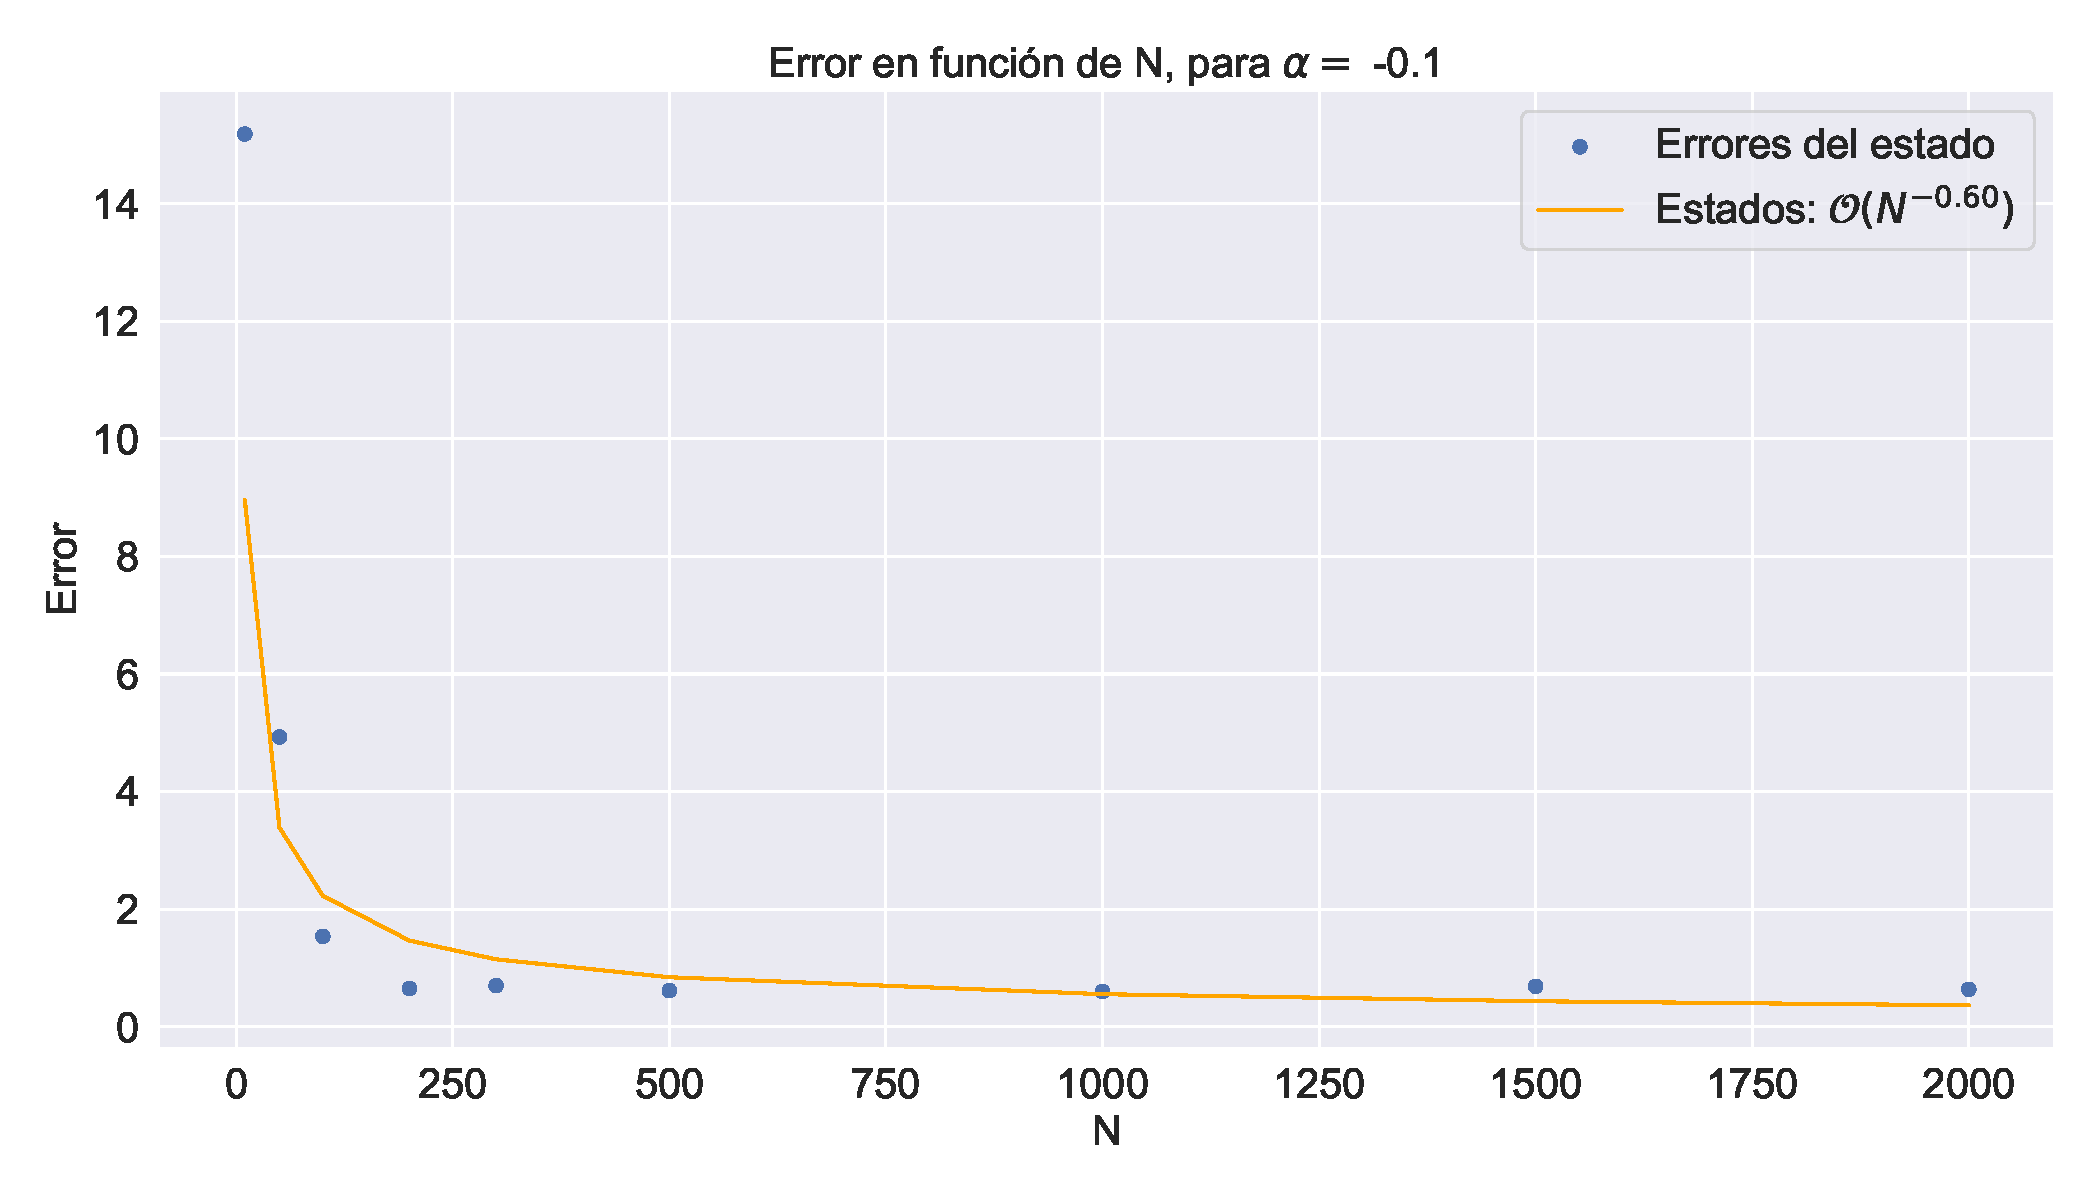
\includegraphics[width=\linewidth]{img/content/chapter4/linear_error_01.pdf}
    \caption{$\alpha = -0.1$}
    \label{fig:linear_error_01}
    \end{subfigure}
     \begin{subfigure}[b]{0.49\textwidth}
         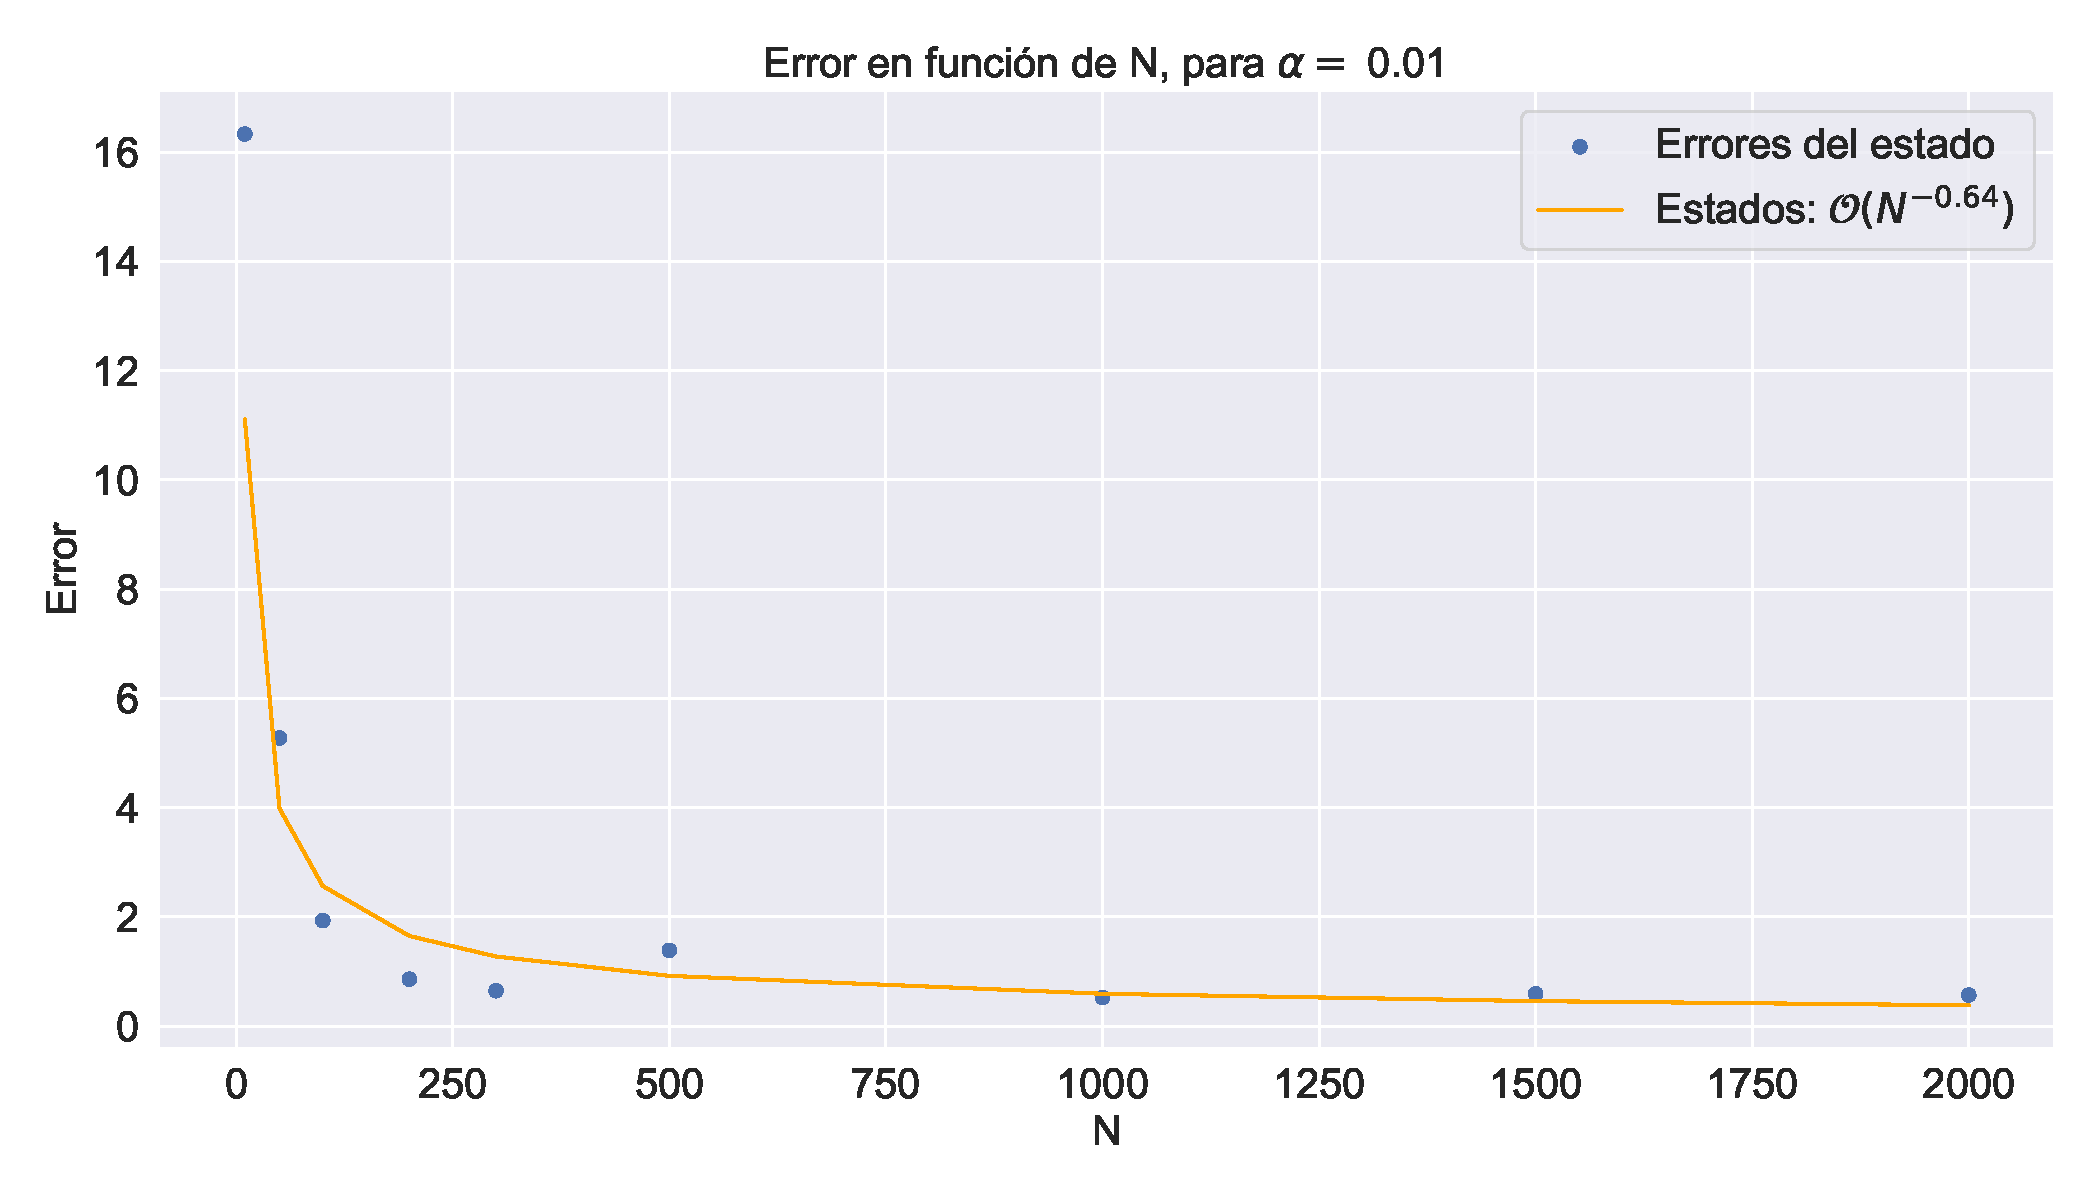
\includegraphics[width=\linewidth]{img/content/chapter4/linear_error_001.pdf}
    \caption{$\alpha = 0.01$}
    \label{fig:linear_error_001}
    \end{subfigure}
     \begin{subfigure}[b]{0.49\textwidth}
        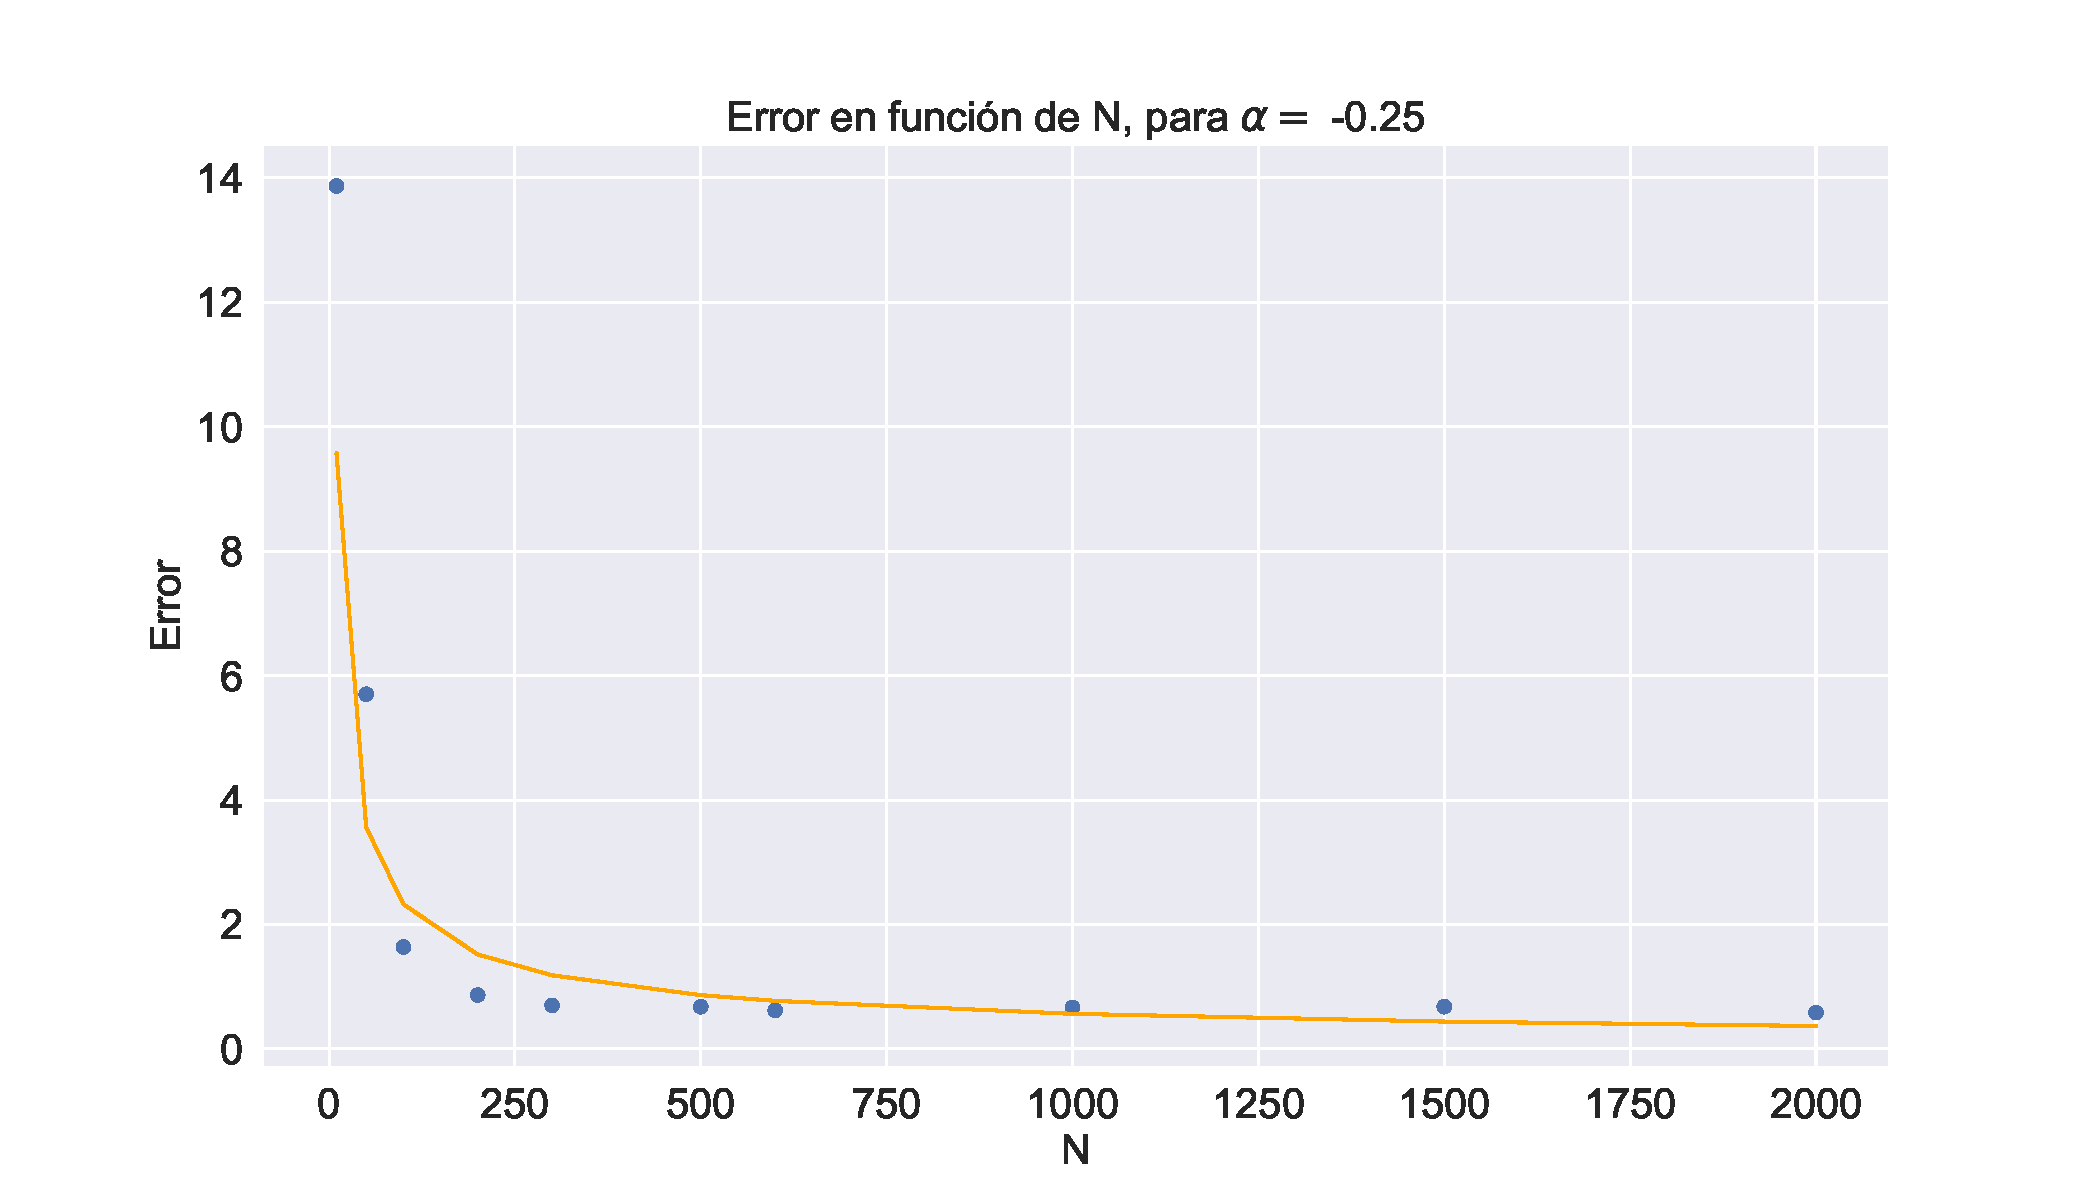
\includegraphics[width=\linewidth]{img/content/chapter4/linear_error_025.pdf}
    \caption{$\alpha = -0.25$}
    \label{fig:linear_error_025}
    \end{subfigure}    
    \caption{Error en norma para el estado en función de $N$ para distintos valores de $\alpha$.}
\end{figure}

\subsection{Comparación para modelos epidemiológicos con otros filtros}

Ahora se compara el filtro con otros filtros no lineales presentados en los preliminares, que vendrían siendo Extended Kalman Filter (EKF), Unscented Kalman Filter (UKF) y Particle Filters (PF), que, tal como se mencionó antes, son implementación propia para este trabajo. 

El sistema a considerar es el sistema SIR ya visto anteriormente
\begin{equation*}
    \begin{aligned}
    S_{k+1} &= S_k -\beta S_k I_k, \\
    I_{k+1} &= I_k + \beta S_k I_k - \gamma I_k, \\
    S_{k+1} &= R_k + \gamma I_k,
    \end{aligned}
\end{equation*}
en donde para esta subsección se considerarán $\beta$ y $\gamma$ conocidos y que la función de observación es
\begin{equation*}
    \mathbf{g}(S, I, R) = I,
\end{equation*}
es decir, solo se observan los infectados.

Se estudia primero el caso en que se prueban los filtros para $\beta = 1.0$ y $\gamma = 0.3$ y ruidos normales centrados con matrices de covarianza
\begin{equation*}
    \mathbf{Q} = \text{diag}(\sigma, \sigma, \sigma), \quad \mathbf{R} = \text{diag}(\sigma),
\end{equation*}
en donde $\sigma$ variará en cada experimento para poder visualizar cómo se comporta cada filtro en presencia de mayor ruido.

Se utiliza como condición inicial real $\mathbf{x}_0 = (0.9, 0.1, 0.0)$, prior para la condición inicial una variable aleatoria normal centrada en $\hat{\mathbf{x}}_0 = (0.9, 0.05, 0.05)$ con matriz de covarianza $\mathbf{Q}_0 = (0.01, 0.01, 0.01)$. Para el EKF se utilizan diferencias finitas centradas para la aproximación del Jacobiano de la dinámica con precisión $\varepsilon=10^{-6}$, para PF se utilizaron $N_p = 5000$ partículas y para KKF se utilizó $N=1000$ como dimensión de aproximación de los operadores. En las figuras \ref{fig:nonlinear_filters_sir_sigma_01}, \ref{fig:nonlinear_filters_sir_sigma_001} y \ref{fig:nonlinear_filters_sir_sigma_0001} se observan los resultados para $\sigma \in \{0.1, 0.01, 0.001\}$, seguido de las tablas \ref{tab:errores_sigma_01}, \ref{tab:errores_sigma_001} y \ref{tabla:errores_sigma_0001} que contienen el detalle de los errores para cada estado y cada filtro.

\begin{figure}[h!]
    \centering
    \begin{subfigure}[b]{0.49\textwidth}
        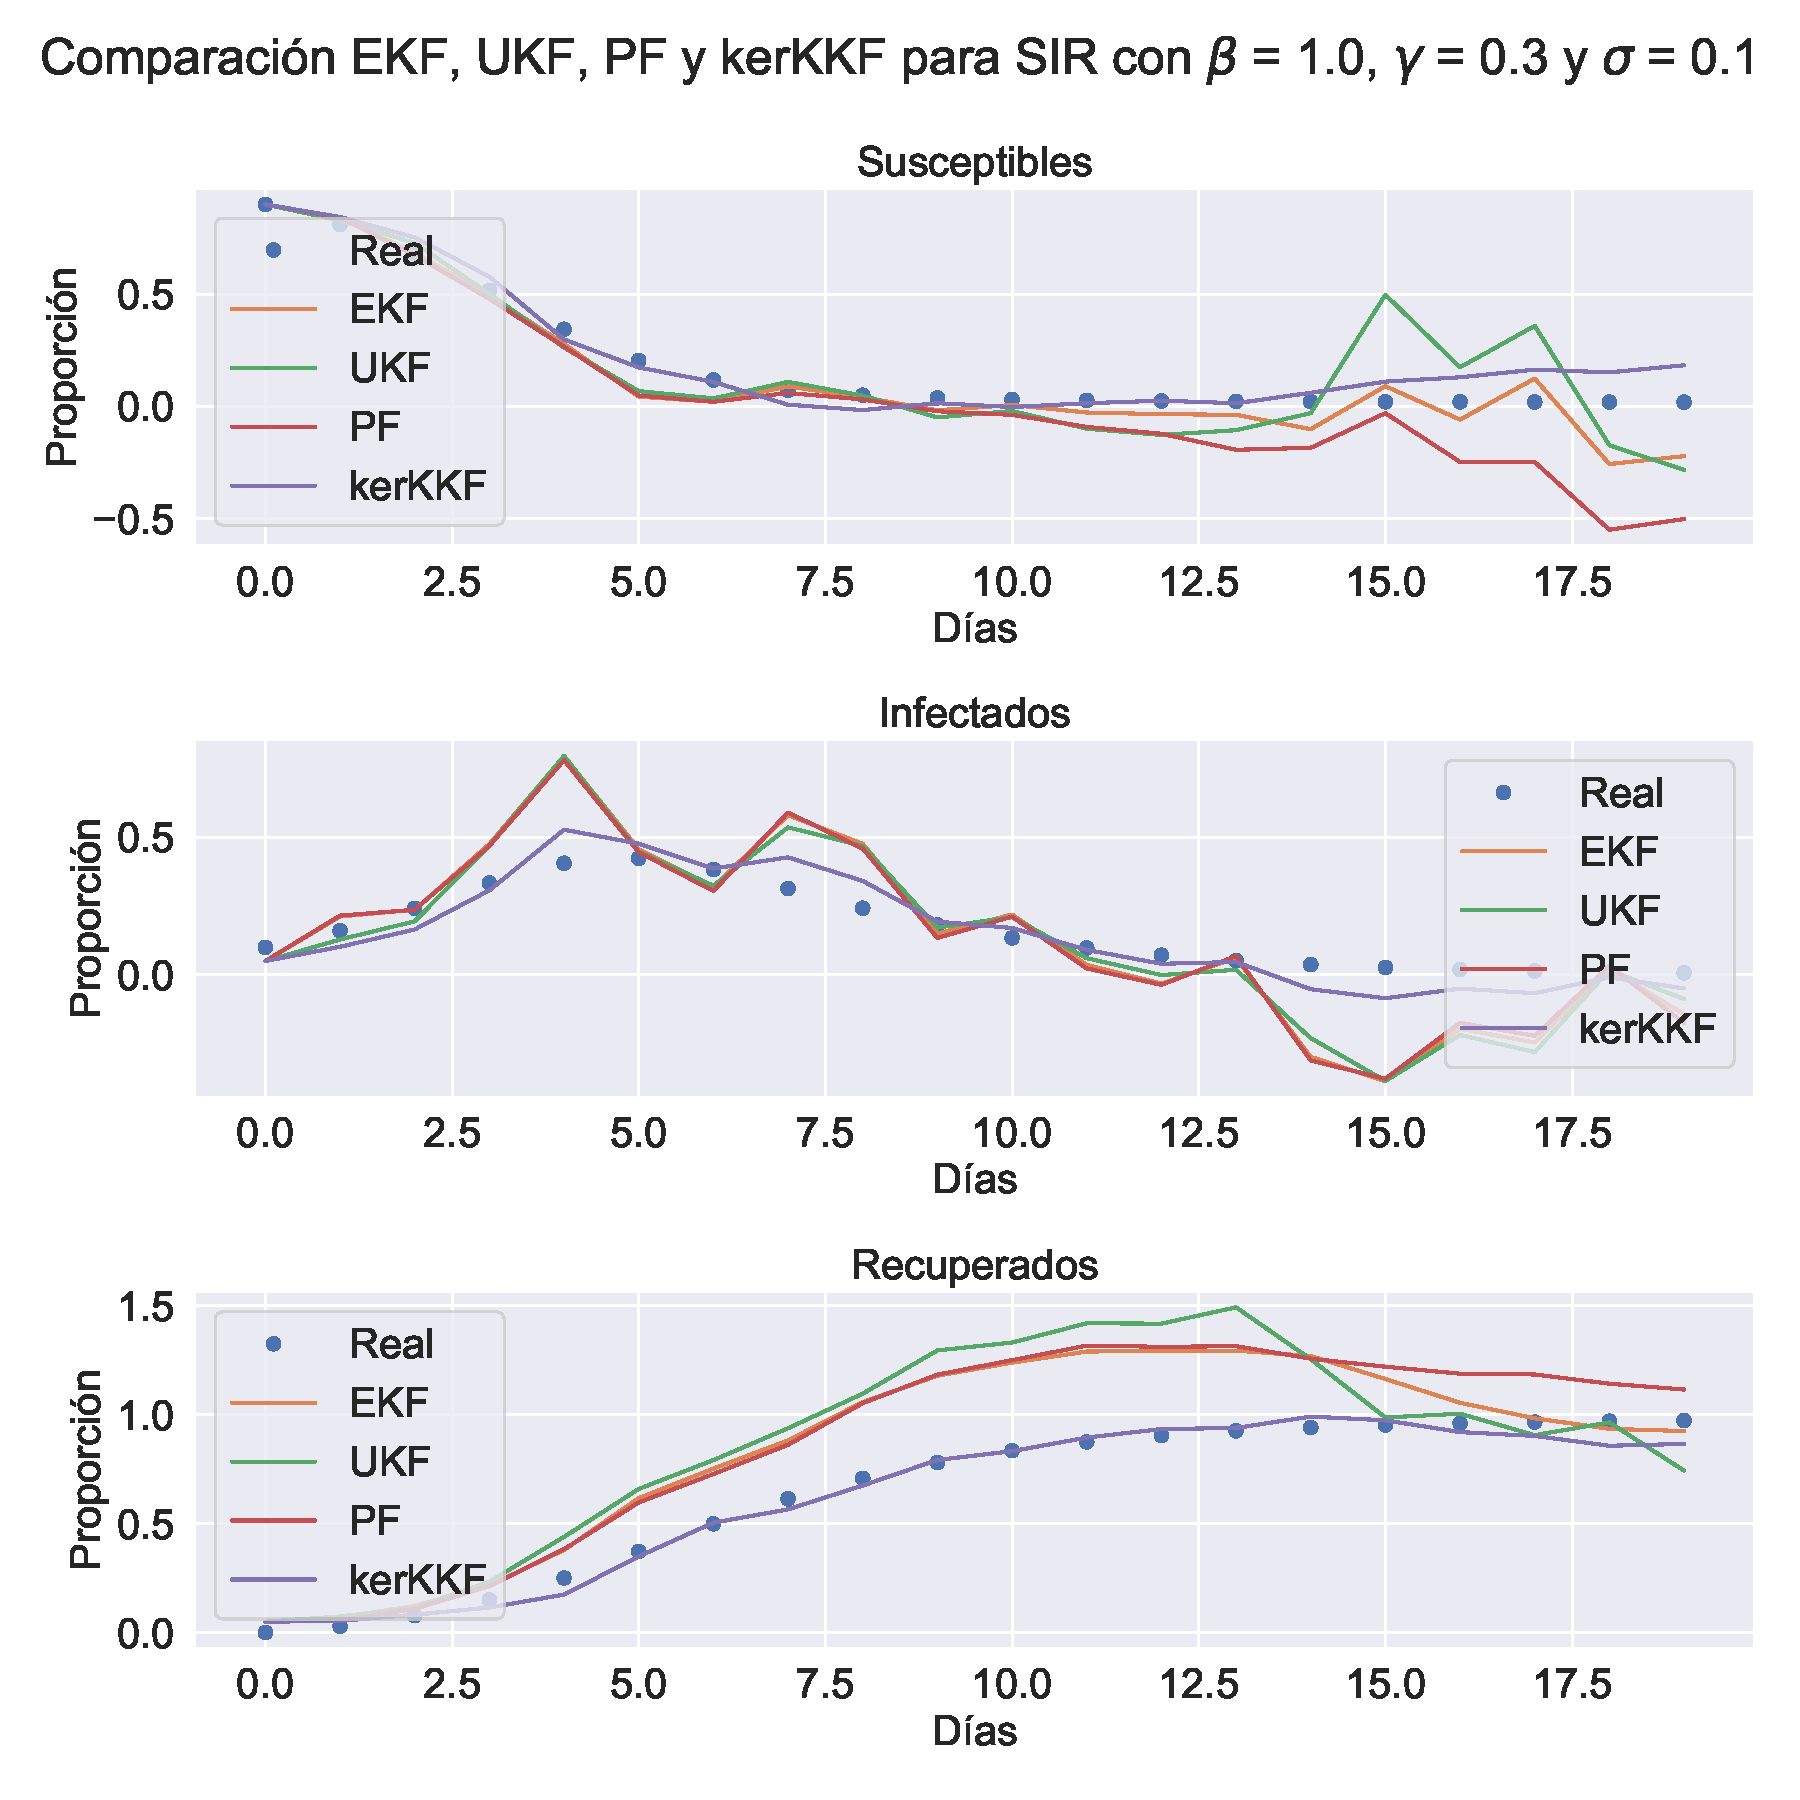
\includegraphics[width=0.9\linewidth]{img/content/chapter4/nonlinear_filters_sir_sigma_01.pdf}
    \caption{$\sigma = 0.1$.}
    \label{fig:nonlinear_filters_sir_sigma_01}
    \end{subfigure}
    \begin{subfigure}[b]{0.49\textwidth}
        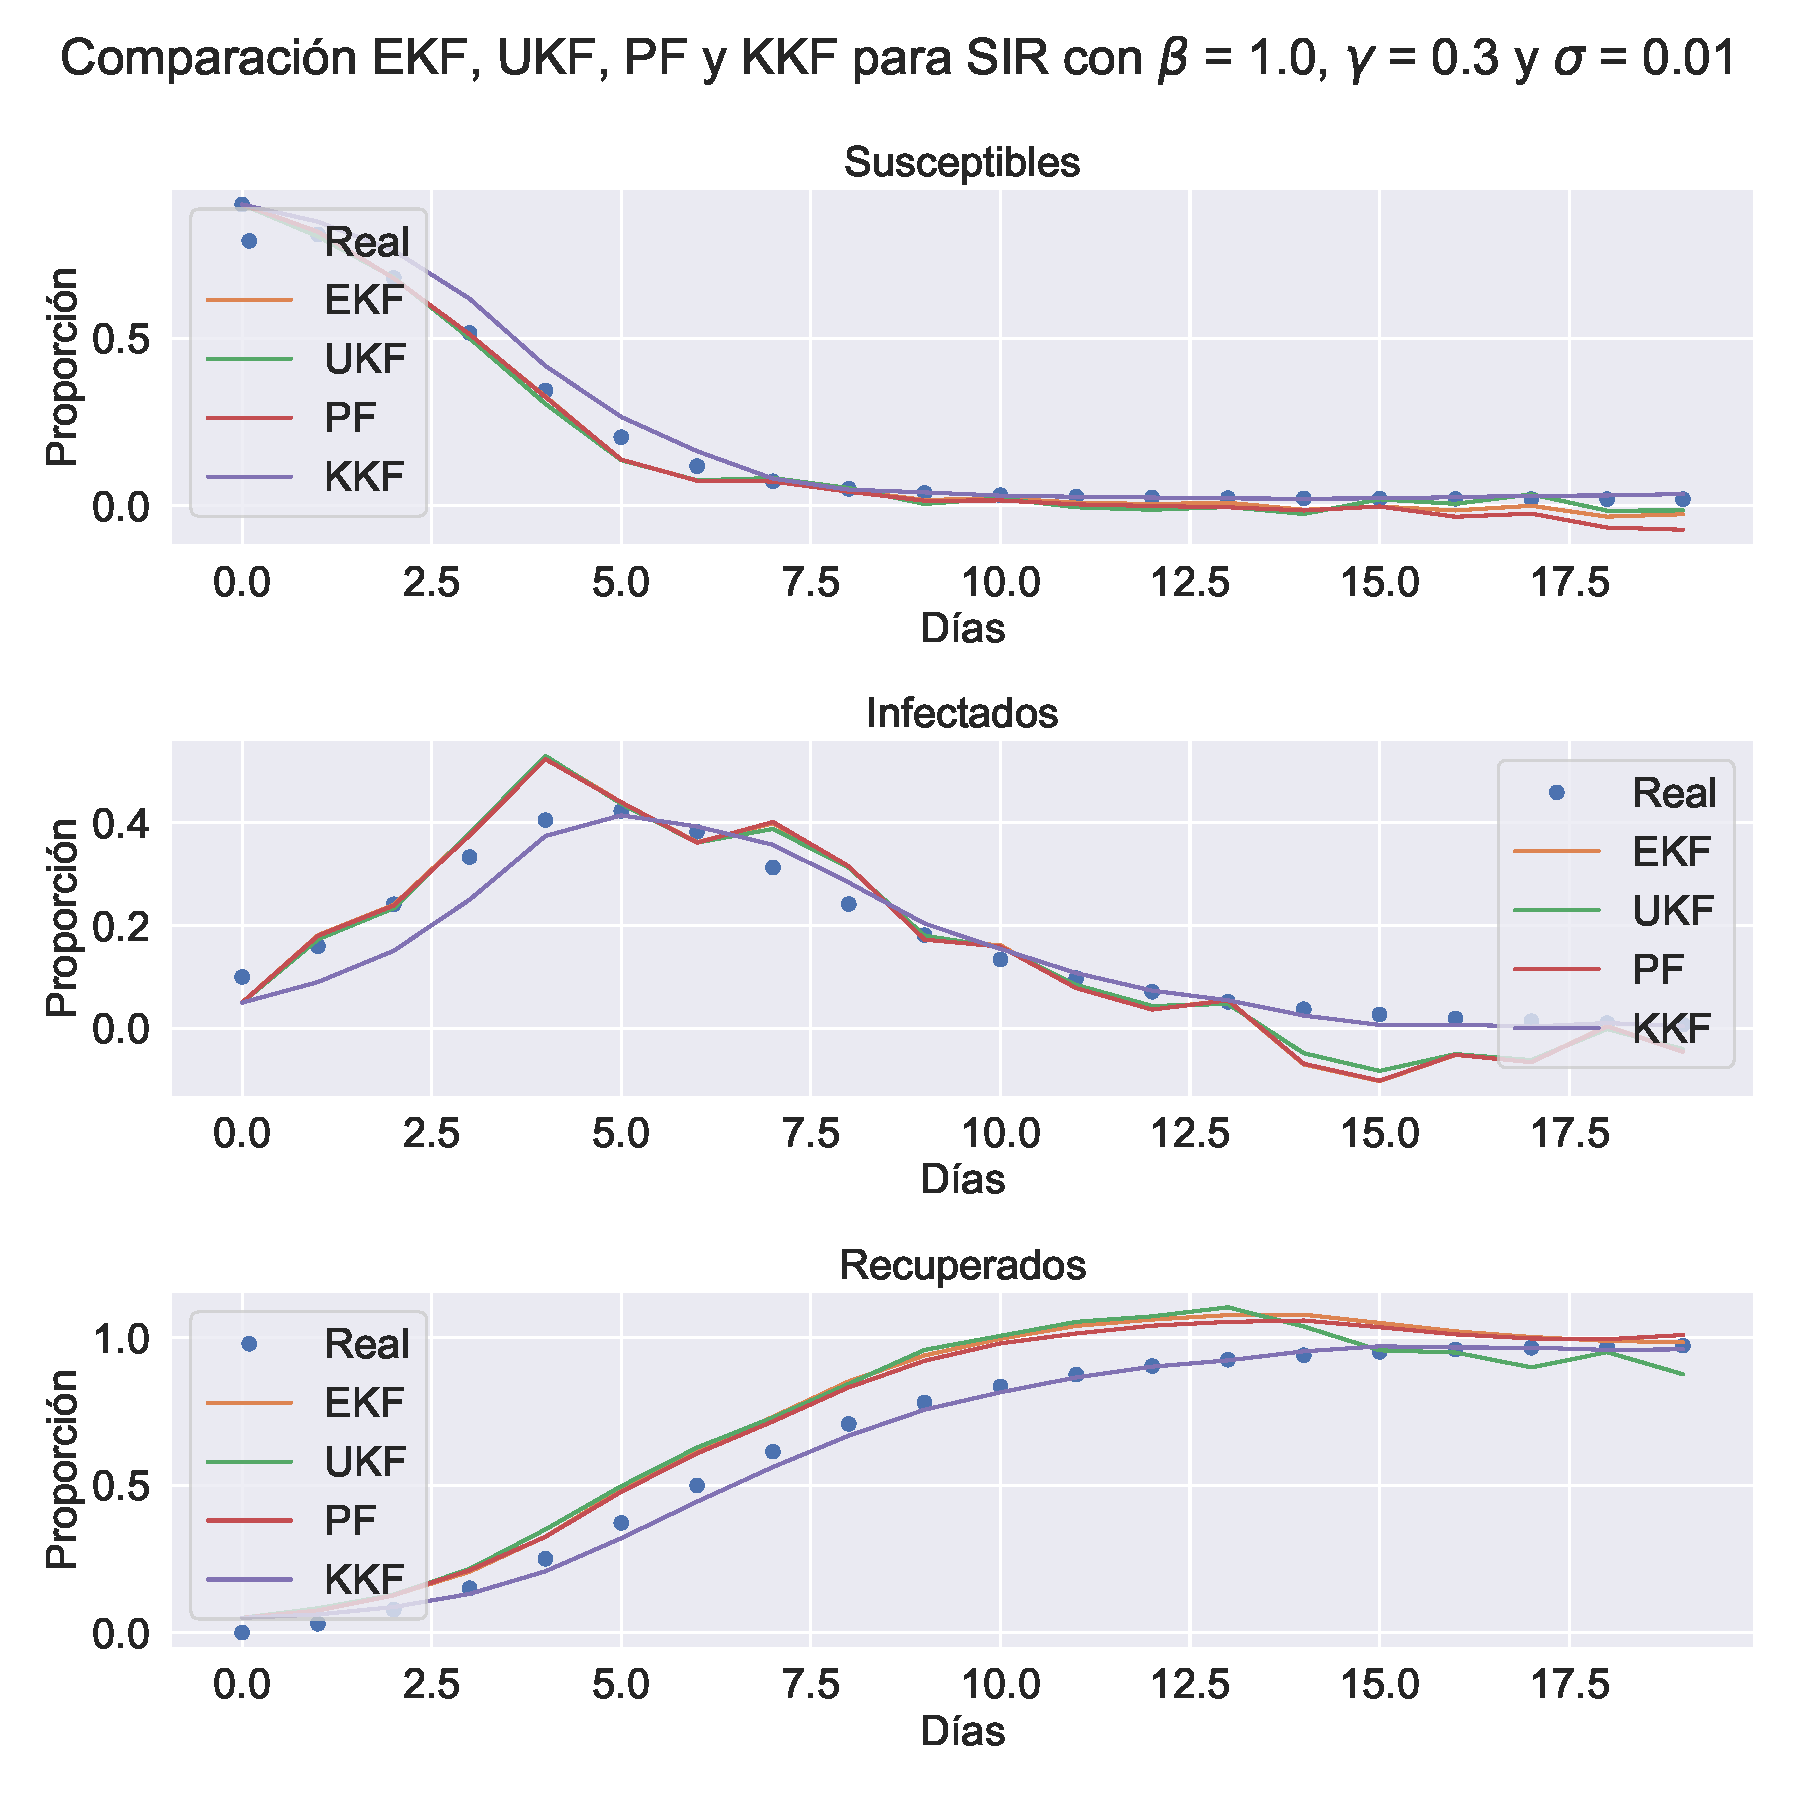
\includegraphics[width=0.9\linewidth]{img/content/chapter4/nonlinear_filters_sir_sigma_001.pdf}
    \caption{$\sigma = 0.01$.}
    \label{fig:nonlinear_filters_sir_sigma_001}
    \end{subfigure}
    \begin{subfigure}[b]{0.49\textwidth}
        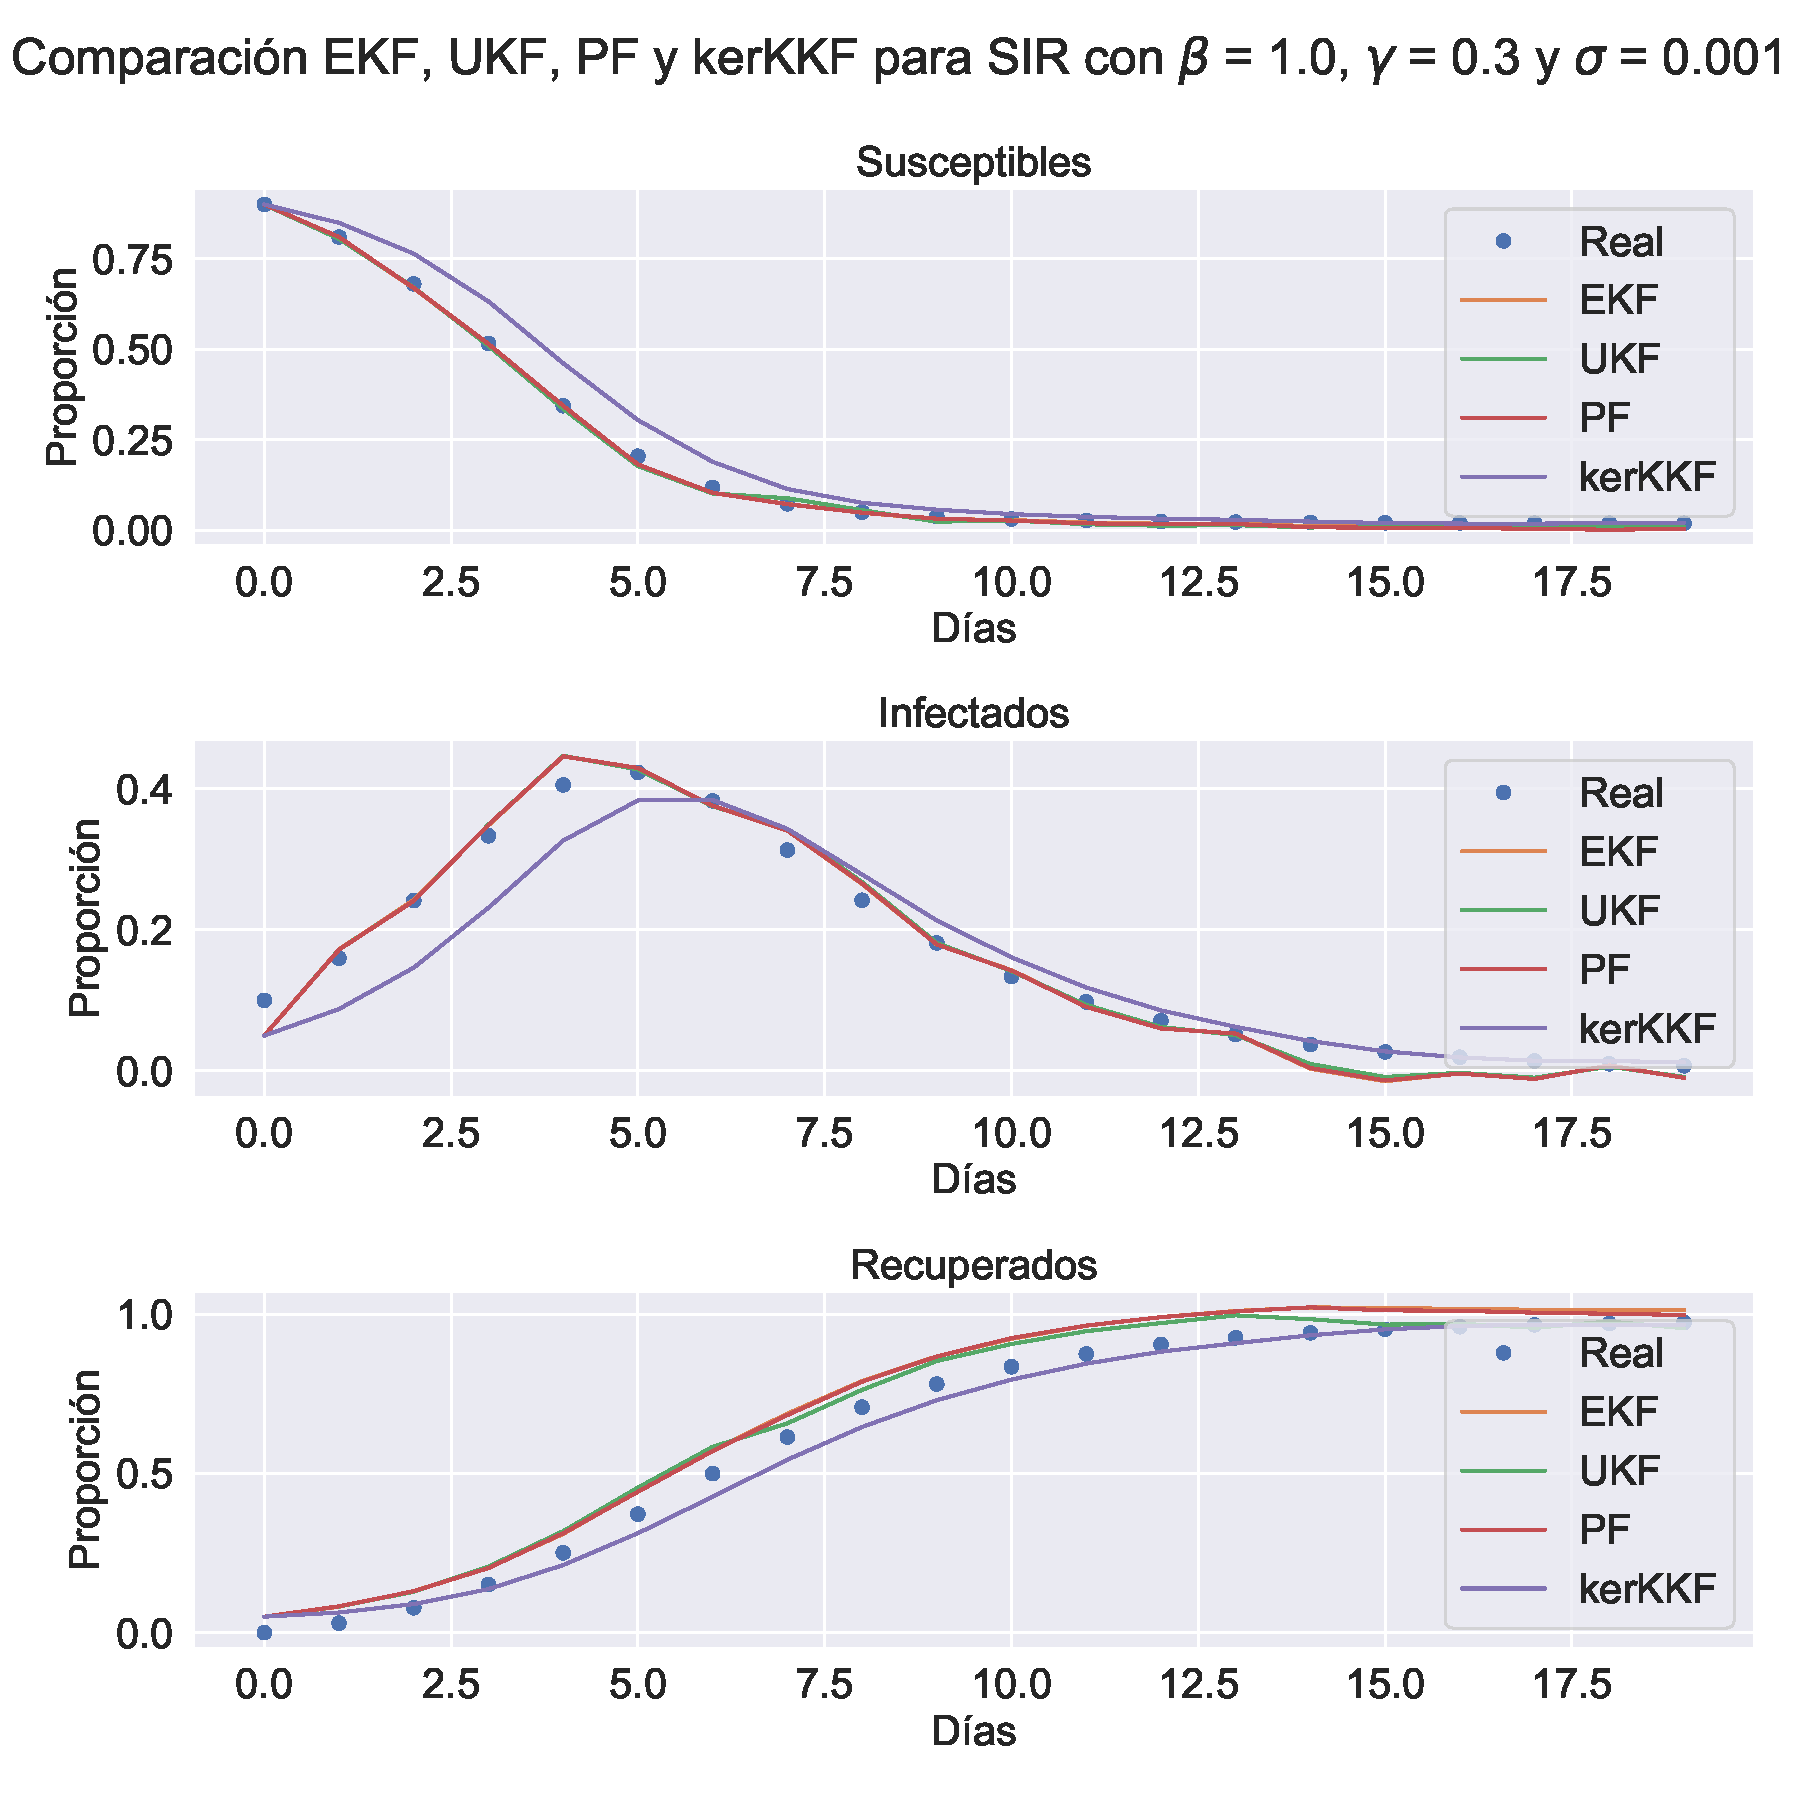
\includegraphics[width=0.9\linewidth]{img/content/chapter4/nonlinear_filters_sir_sigma_0001.pdf}
    \caption{$\sigma = 0.001$.}
    \label{fig:nonlinear_filters_sir_sigma_0001}
    \end{subfigure}
    \caption{Comparación de resultados de las trayectorias generadas por los filtros EKF (naranja), UKF (verde), PF (rojo) y KKF (púrpura), junto con la trayectoria real (puntos azules) sin ruidos, ni de dinámica ni de observación, esto para cada uno de los estados del modelo SIR. $\sigma$ es variable para (a), (b) y (c), mientras que $\beta = 1.0$ y $\gamma = 0.3$ fijos.}
\end{figure}

\begin{table}[h!]
    \caption{Errores de los distintos filtros con respecto a la trayectoria real, para distintos valores de la diagonal de la matriz de covarianza del ruido de dinámica $\sigma$.}
    \begin{subtable}{\linewidth}
        \centering
    \caption{$\sigma = 0.1$}
    \begin{tabular}{|c|c|c|c|c|}
    \hline
    \textbf{Estado} & \textbf{EKF} & \textbf{UKF} & \textbf{PF} & \textbf{KKF} \\ \hline
    S & 0.4757 & 0.7738 & 0.9571 & 0.3330 \\ \hline
    I & 0.8665 & 0.8300 & 0.8553 & 0.3015 \\ \hline
    R & 1.1360 & 1.4221 & 1.2151 & 0.2209 \\ \hline
    \end{tabular}
    \label{tab:errores_sigma_01}
    \end{subtable}
    \begin{subtable}{\linewidth}
        \centering
    \caption{$\sigma = 0.01$}
    \begin{tabular}{|c|c|c|c|c|}
    \hline
    \textbf{Estado} & \textbf{EKF} & \textbf{UKF} & \textbf{PF} & \textbf{KKF} \\ \hline
    S & 0.1277 & 0.1328 & 0.1783 & 0.1737 \\ \hline
    I & 0.2801 & 0.2565 & 0.2779 & 0.1709 \\ \hline
    R & 0.4881 & 0.5135 & 0.4337 & 0.1329 \\ \hline
    \end{tabular}
    \label{tab:errores_sigma_001}
    \end{subtable}
    \begin{subtable}{\linewidth}
        \centering
    \caption{$\sigma = 0.001$}
    \begin{tabular}{|c|c|c|c|c|}
    \hline
    \textbf{Estado} & \textbf{EKF} & \textbf{UKF} & \textbf{PF} & \textbf{KKF} \\ \hline
    S & 0.0417 & 0.0528 & 0.0493 & 0.2320 \\ \hline
    I & 0.1023 & 0.0985 & 0.1022 & 0.1996 \\ \hline
    R & 0.3070 & 0.2489 & 0.2983 & 0.1710 \\ \hline
    \end{tabular}
    \label{tabla:errores_sigma_0001}
    \end{subtable}
\end{table}

Se observa que KKF logra superar en error a todos los otros filtros con creces en el caso en que $\sigma \in \{ 0.1, 0.01\}$, aunque para el caso en donde hay menor ruido los resultados son bastante similares. Esto mostraría que el filtro tiene un mejor desempeño en comparación con los otros filtros en escenarios de mayor incertidumbre.

Se muestra ahora el caso en que $\sigma = 0.01$ fijo y varía el parámetro $\beta \in \{0.6, 0.9, 1.5\}$, en donde el objetivo es ver cómo cambian los resultados en función de $\beta$, que es en algún sentido el parámetro que cuantifica la no linealidad del sistema. Dado que $\gamma$ en realidad representa una relación lineal, se deja fijo en $\gamma = 0.3$. Se utilizan los mismos valores para todo el resto de configuraciones. Los resultados se pueden apreciar en las figuras \ref{fig:nonlinear_filters_sir_beta_06}, \ref{fig:nonlinear_filters_sir_beta_09} y \ref{fig:nonlinear_filters_sir_beta_15}, y en las tablas \ref{tab:errores_beta_gamma_06}, \ref{tab:errores_beta_gamma_09} y \ref{tab:errores_beta_gamma_15}.

Además, se midió el error en norma de los filtros para $50$ valores de $\beta$ entre $0.1$ y $2.5$ equiespaciados, manteniendo todo el resto de parámetros sin cambios. El resultado se puede observar en la figura \ref{fig:nonlinear_filters_sir_error_beta}, en donde KKF tiene un mejor desempeño a nivel general.

\subsection{Estimación de parámetros de modelos epidemiológicos}

A continuación se prueba la metodología para estimación de parámetros, que se compara con Markov Chain Monte Carlo, utilizando como \textit{samplers} Differential Evolution Metropolis (DEMetropolisZ) \cite{terBraak2008DifferentialChains}, que es un \textit{sampler} no basado en gradiente, y No-U-Turn Sampler (NUTS) \cite{Hoffman2014TheCarlo}, que está basado en gradiente y además es de los más utilizados cuando hay un sistema dinámico subyacente implementado en PyMC \cite{Patil2010PyMC:Python}.

Para DEMetropolisZ se utilizarán 20000 iteraciones de \textit{warm up}, es decir, no se utilizarán para la estimación y 20000 para estimación como tal. Mientras que para NUTS se utilizaron 150 y 150, respectivamente. Para la aproximación de Koopman, en los tres sistemas donde se probó, se utilizará $N=100$. Se realizaron 300 iteraciones del algoritmo \ref{alg:ParamEstim}, de las cuales la primera mitad se tomó como \textit{warm up} y la segunda mitad se considerará para la estimación. Para los 3 algoritmos, se hará el mismo procedimiento 8 veces en paralelo.

Se prueba la metodología de estimación de parámetros para el modelo SIR \eqref{eq:SIR}, esto es, lograr una estimación para $\beta$ y $\gamma$ en base a observaciones, tal como se encuentra en el algoritmo \ref{alg:ParamEstim}. Por lo que se considera el modelo con estados aumentados, que es

\begin{equation*}
    \begin{aligned}
        S_{k+1} &= S_k - \beta_k S_k I_k + \mathbf{w}_k^1 \\
        I_{k+1} &= I_k + \beta_k S_k I_k - \gamma_k I_k + \mathbf{w}_k^2 \\
        R_{k+1} &= R_k + \gamma_k I_k + \mathbf{w}_k^3 \\
        \beta_{k+1} &= \beta_k + \mathbf{w}_k^4 \\
        \gamma_{k+1} &= \gamma_k + \mathbf{w}_k^5
    \end{aligned}
\end{equation*}

Se utilizan como parámetros reales $\beta=1.3$ y $\gamma=0.5$, se utiliza como condición inicial para el estado aumentado $\mathbf{x}_0 = (0.9, 0.1, 0.0, 1.3, 0.5)$, y se entrega también como media del prior de la condición inicial $\hat{\mathbf{x}}_0 = (0.9, 0.1, 0.0, 0.1, 0.1)$, con matriz de covarianza inicial
\begin{equation*}
    \mathbf{Q}_0 = \text{diag}(0.001, 0.001, 0.001, 1, 1).
\end{equation*}

Es decir, se entrega como condición inicial para los parámetros $0.1$ y se espera que el algoritmo converja a los parámetros reales. Se considera que los estados observables son $S$ e $I$, es decir
\begin{equation*}
    \mathbf{g}(S, I, R, \beta, \gamma) = (S, I)
\end{equation*}
y se consideran ruidos normales aditivos, centrados y con matrices de covarianza, para la dinámica y la observación, respectivamente
\begin{equation*}
    \mathbf{Q} = \text{diag}(0.001, 0.001, 0.001, 1, 1), \quad \mathbf{R} = \text{diag}(0.001, 0.001).
\end{equation*}

Se simula el sistema a $20$ unidades de tiempo y para muestrear puntos desde el estado se utiliza una variable aleatoria cuyas primeras tres entradas vienen desde una Dirichlet de parámetro $(1,1,1)$ y las otras dos desde Uniformes en $[0.5, 1.5]$ y $[0.1, 0.5]$, respectivamente. 

Se realizan $300$ iteraciones para el procedimiento expuesto en el algoritmo \ref{alg:ParamEstim}. Este procedimiento se hace $8$ veces en paralelo, por lo que hay $8$ filtros, que se denotarán cadenas, que están estimando el parámetro en paralelo. 

En la figura \ref{fig:param_estim_SIR} se muestra el resultado del filtro en la última iteración y la evolución del parámetro estimado en función de las iteraciones, todo esto solo para la primera cadena de manera ilustrativa. En la figura \ref{fig:density_param_estim_SIR} se muestran las densidades de probabilidad generadas por cada cadena, comparadas con el valor real del parámetro. Si estas se promedian, queda una densidad de probabilidad que es mucho más robusta para la estimación del parámetro, resultado que se puede observar en la figura \ref{fig:mean_density_param_estim_SIR}.



\begin{figure}[h!]
    \centering
    \begin{subfigure}[b]{0.8\textwidth}
        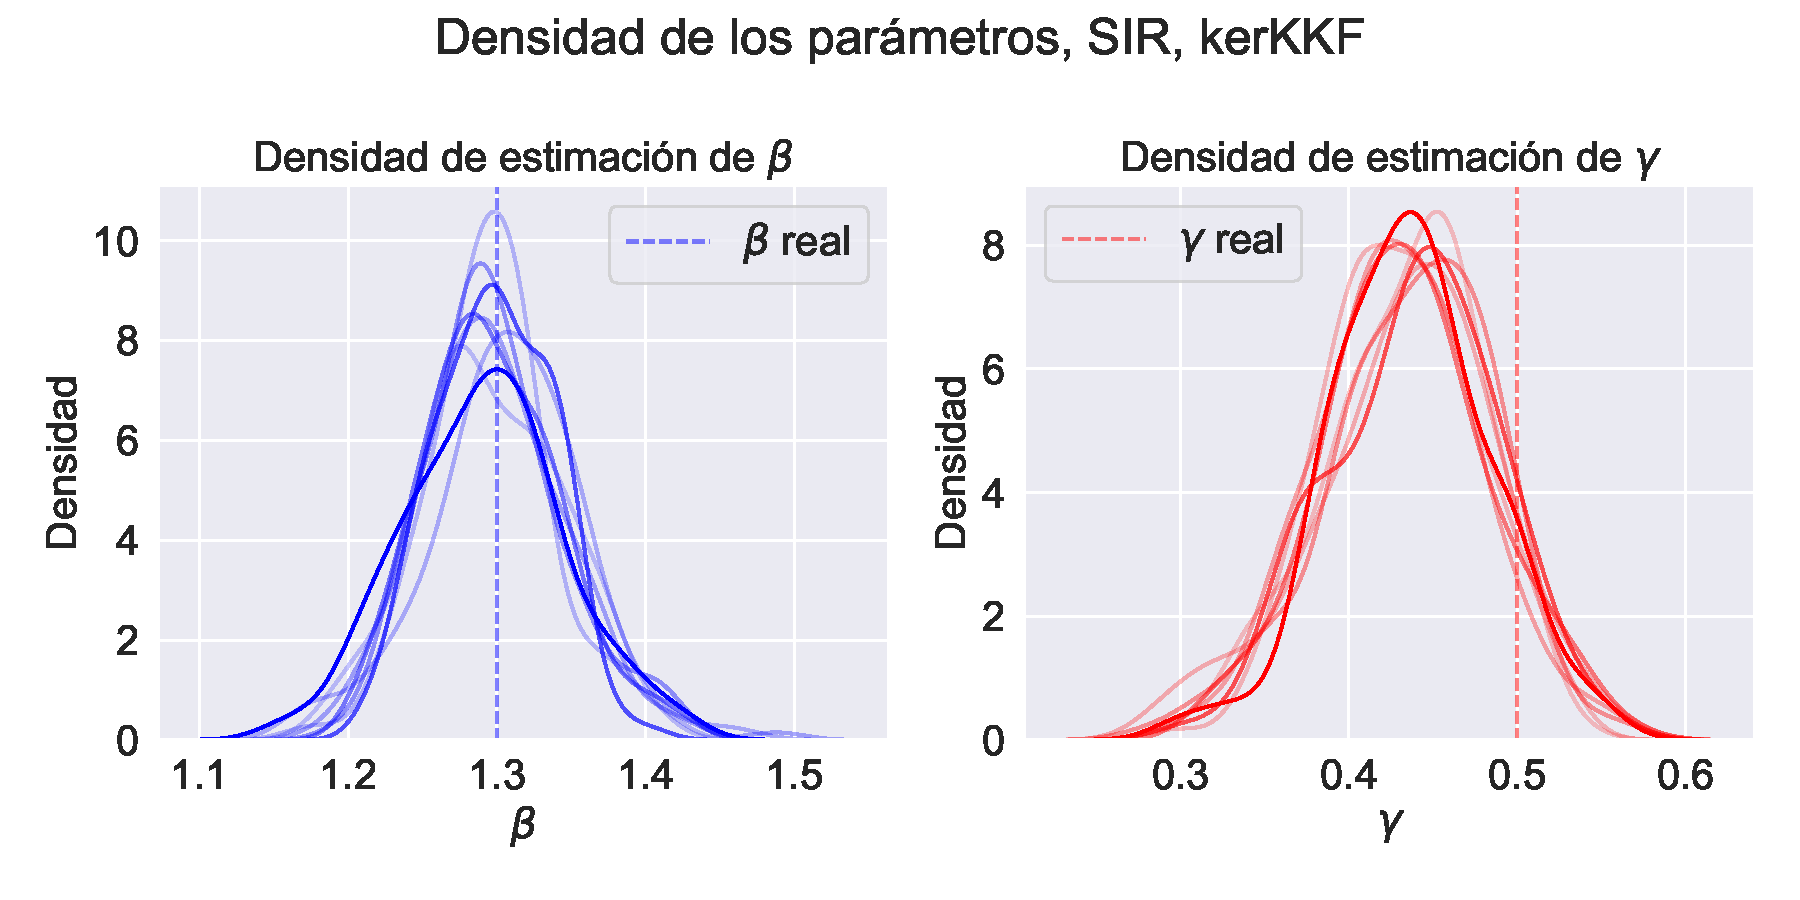
\includegraphics[width=\linewidth]{img/content/chapter4/nonlinear_filters_sir_params_density.pdf}
        \caption{}
        \label{fig:density_param_estim_SIR}
    \end{subfigure}
    \begin{subfigure}[b]{0.8\textwidth}
        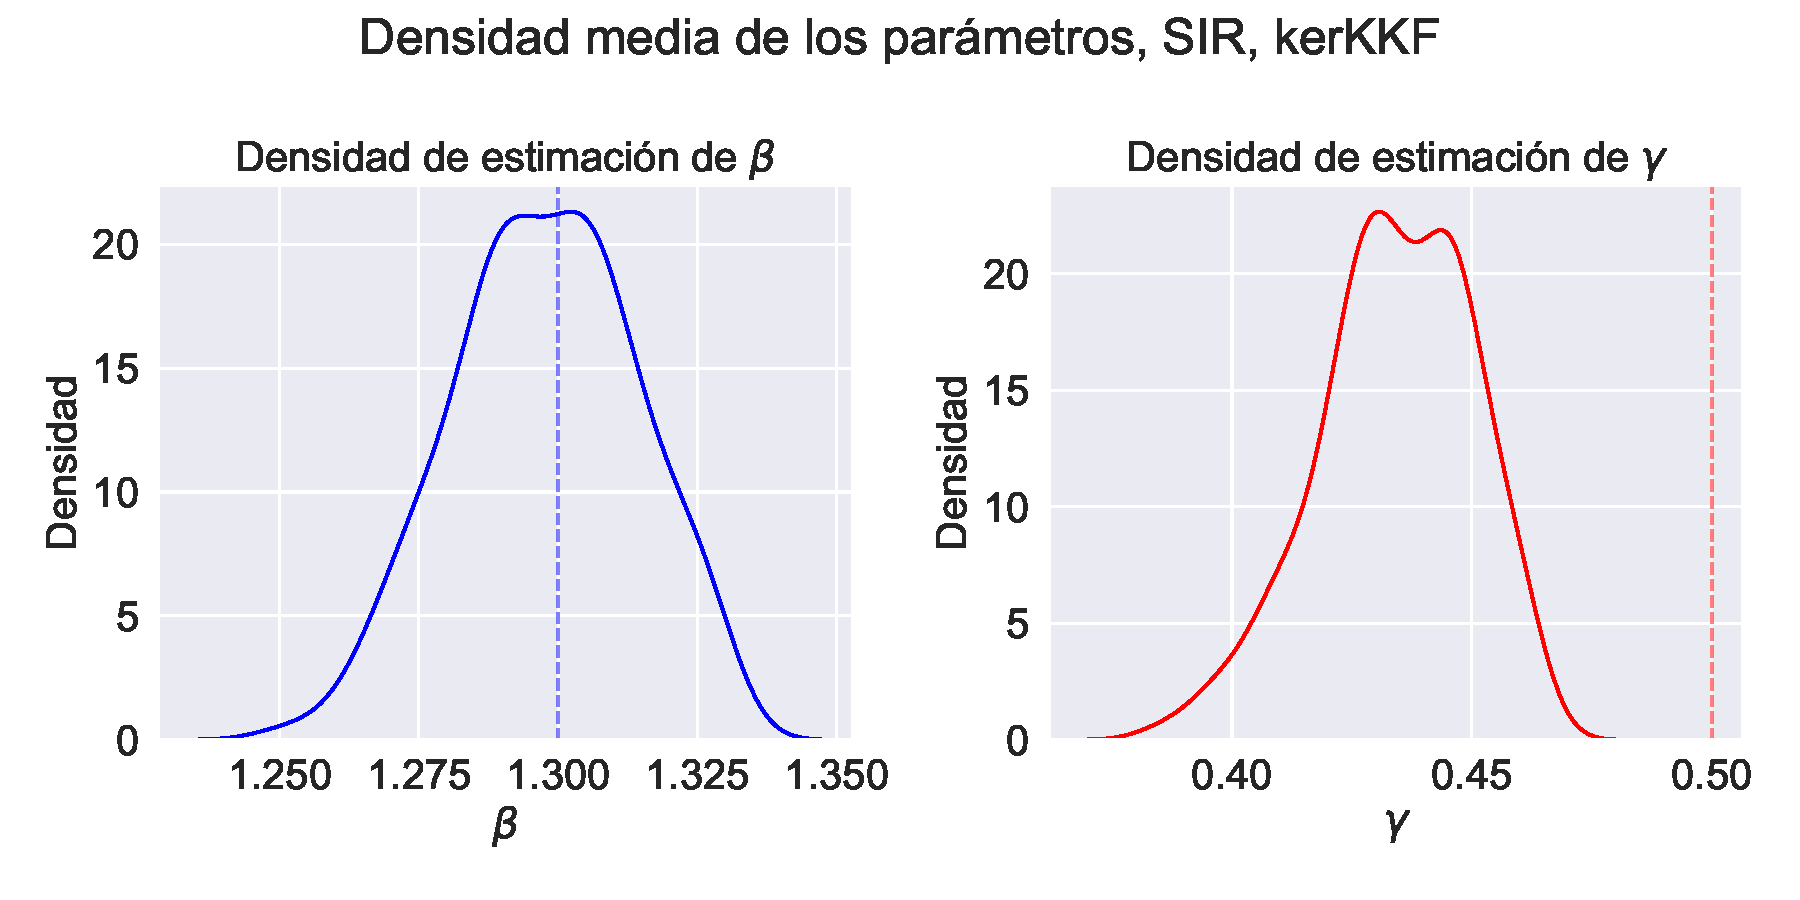
\includegraphics[width=\linewidth]{img/content/chapter4/nonlinear_filters_sir_params_density_mean.pdf}
        \caption{}
        \label{fig:mean_density_param_estim_SIR}
    \end{subfigure}
    \caption{A la izquierda el resultado para $\beta$ y a la derecha para $\gamma$, parámetros del modelo SIR \eqref{eq:SIR}. En línea punteada vertical se encuentra el valor real del parámetro. \\
    (a) Densidades de probabilidad creadas por cada cadena solo considerando las iteraciones posteriores al \textit{warm up}. Por cada una son $8$ densidades correspondientes a cada cadena. \\
    (b) Densidades de probabilidad resultante de promediar las $8$ densidades creadas por cada cadena.}
    
\end{figure}

Se repite el mismo procedimiento con el modelo SIRS para estimar sus parámetros $\alpha$, $\beta$ y $\gamma$, que con el estado aumentado queda
\begin{equation*}
    \begin{aligned}
        S_{k+1} &= S_k - \beta_k S_k I_k + \alpha_k R_k + \mathbf{w}_k^1 \\
        I_{k+1} &= I_k + \beta_k S_k I_k - \gamma_k I_k + \mathbf{w}_k^2 \\
        R_{k+1} &= R_k + \gamma_k I_k - \alpha_k R_k + \mathbf{w}_k^3 \\
        \alpha_{k+1} &= \alpha_k + \mathbf{w}_k^4 \\
        \beta_{k+1} &= \beta_k + \mathbf{w}_k^5 \\
        \gamma_{k+1} &= \gamma_k + \mathbf{w}_k^6.
    \end{aligned}
\end{equation*}

Para el experimento se utilizaron como valores reales reales $\alpha = 0.2$, $\beta = 1.4$, $\gamma = 0.4$ y condición inicial para el resto de estados $(S_0, I_0, R_0) = (0.9, 0.1, 0.0)$. Se entrega como prior para la condición inicial una normal centrada en $\hat{\mathbf{x}}_k = (0.9, 0.1, 0.0, 0.1, 0.1, 0.1)$ con matriz de covarianza
\[
\mathbf{Q}_0 = \text{diag}(0.01, 0.01, 0.01, 10, 10, 10).
\]

Como función de observación ahora se considera que únicamente es posible observar a los infectados, es decir
\[
\mathbf{g}(S, I, R, \alpha, \beta, \gamma) = I,
\]
por lo que se tiene menos información incluso para este caso que para el anterior, en que se deseaba estimar menos parámetros.

Como distribuciones asociadas a la dinámica y la observación se utiliza un ruido normal aditivo, centrado y con matriz de covarianza y varianza, respectivamente
\[
\mathbf{Q} = \text{diag}(0.001, 0.001, 0.001, 10, 10, 10), \quad \mathbf{R} = 0.01
\]
dado que para la observación es necesaria una variable univariada.

Para muestrear desde el estado se utiliza una variable aleatoria cuyas primeras tres entradas provienen de una Dirichlet de parámetro $(1,1,1)$ y las otras tres de variables aleatorias uniformes en $[0.1, 1.0]$, $[0.1, 0.5]$ y $[0.1, 0.5]$, respectivamente. Se simula el sistema a $20$ unidades temporales.

En la figura \ref{fig:nonlinear_filters_sirs_params} se observa la solución de KKF para el sistema, esto para la última iteración del algoritmo \ref{alg:ParamEstim} y en la primera cadena de las $8$ muestreadas, mientras que en la figura \ref{fig:nonlinear_filters_sirs_params_evolution} se puede ver la evolución del parámetro a través de las iteraciones, esto también para la primera cadena.

Análogo a lo hecho antes, se puede convertir la evolución del parámetro a través de las iteraciones del algoritmo en una densidad de probabilidad, para la cual se consideran solo la segunda mitad de las iteraciones, dejando la primera mitad como \textit{warm up}. Esto se puede ver en la figura \ref{fig:nonlinear_filters_sirs_params_density}, en donde se dejan las $8$ cadenas y en la figura \ref{fig:nonlinear_filters_sirs_params_density_mean} la cadena media para cada uno de los parámetros.

El algoritmo logra acercarse mucho a los parámetros reales de cada sistema, dejando al menos el parámetro real en su intervalo de confianza de nivel $95$\%.

Por último, se prueba para el modelo SEIR, que tiene 4 estados y 4 parámetros por estimar, $\alpha$, $\beta$, $\gamma$ y $\delta$.
\begin{equation*}
    \begin{aligned}
        S_{k+1} &= S_k - \beta_k S_k I_k + \alpha_k R_k + \mathbf{w}_k^1 \\
        E_{k+1} &= E_k + \beta_k S_k I_k - \delta_k E_k + \mathbf{w}_k^2 \\
        I_{k+1} &= I_k + \delta_k E_k - \gamma_k I_k + \mathbf{w}_k^3 \\
        R_{k+1} &= R_k + \gamma_k I_k - \alpha_k R_k + \mathbf{w}_k^4 \\
        \alpha_{k+1} &= \alpha_k + \mathbf{w}_k^5 \\
        \beta_{k+1} &= \beta_k + \mathbf{w}_k^6 \\
        \gamma_{k+1} &= \gamma_k + \mathbf{w}_k^7 \\
        \delta_{k+1} &= \delta_k + \mathbf{w}_k^8.
    \end{aligned}
\end{equation*}
Se simula el sistema a $20$ unidades de tiempo suponiendo que solo se observan los susceptibles y los infectados, es decir,
\begin{equation*}
    g(S, E, I, R, \alpha, \beta, \gamma, \delta) = (S, I).
\end{equation*}

Se puede ver en las figuras \ref{fig:nonlinear_filters_seir_params_density} y \ref{fig:nonlinear_filters_seir_params_density_mean} las densidades de probabilidad que se generan al estimar parámetros. Para poder estudiar el error en las trayectorias, se \textit{samplean} 30 muestras de parámetros desde las densidades de probabilidad generadas, con lo que se obtiene error promedio, desviación estándar para el error, error mínimo y error máximo, esto para cada modelo y cada método, lo que se puede observar en las tablas \ref{tab:metricas_traj_SIR}, \ref{tab:metricas_traj_SIRS} y \ref{tab:metricas_traj_SEIR}, mientras que las trayectorias \textit{sampleadas} se pueden encontrar en las figuras \ref{fig:SIR_traj_params}, \ref{fig:SIRS_traj_params} y \ref{fig:SEIR_traj_params}.

Se observa el rendimiento de los 3 algoritmos, para los 3 sistemas, es bastante similar, solo que KKF entrega intervalos de confianza más pequeños. El aspecto más relevante, por lejos, es el hecho de que KKF es mucho más rápido que DEMetropolisZ y NUTS, siendo incluso casi 10 veces más rápido que NUTS para el modelo SEIR. Esto es un aspecto relevante a considerar dado que NUTS, muy utilizado en muchas aplicaciones de modelos epidemiológicos para estimar parámetros, usualmente demora horas para poder ejecutarse y debe llevarse a supercomputadores. Puede que esta nueva metodología sea más eficiente en este sentido y logre aligerar tareas de computo muy tediosas y disminuir las horas de espera.

\begin{table}[h!]
    \centering
    \caption{Estimación de parámetros del modelo SIR (IC 95\%).} 
    \begin{tabular}{|c|c|c|c|c|}
    \hline
    \textbf{Parámetro} & \textbf{Real} & \textbf{DEMetropolisZ} & \textbf{NUTS} & \textbf{KKF}  \\ \hline
    $\beta$ & 1.3 & 1.59 (0.96, 2.22) & 1.33 (1.31, 1.35) & 1.39 (1.35, 1.42) \\ \hline
    $\gamma$ & 0.5 & 0.69 (0.23, 1.16) & 0.45 (0.44, 0.46) & 0.47 (0.45, 0.49) \\ \hline
    \end{tabular}
    \label{tab:SIR_params}
\end{table}

\begin{table}[h!]
    \centering
    \caption{Estimación de parámetros del modelo SIRS (IC 95\%).} 
    \begin{tabular}{|c|c|c|c|c|}
    \hline
    \textbf{Parámetro}& \textbf{Real} & \textbf{DEMetropolisZ} & \textbf{NUTS} & \textbf{KKF}  \\ \hline
    $\alpha$ & 0.2 & 0.31 (-0.25, 0.88) & 0.17 (0.16, 0.18) & 0.19 (0.17, 0.21) \\ \hline
    $\beta$ & 1.3 & 1.4 (0.88, 1.92) & 1.34 (1.31, 1.36) & 1.3 (1.24, 1.36) \\ \hline
    $\gamma$ & 0.5 & 0.57 (0.22, 0.93) & 0.51 (0.50, 0.52) & 0.44 (0.40, 0.48) \\ \hline
    \end{tabular}
    \label{tab:SIRS_params}
\end{table}

\begin{table}[h!]
    \centering
    \caption{Estimación de parámetros del modelo SEIR (IC 95\%).} 
    \begin{tabular}{|c|c|c|c|c|}
    \hline
    \textbf{Parámetro}& \textbf{Real} & \textbf{DEMetropolisZ} & \textbf{NUTS} & \textbf{KKF}  \\ \hline
    $\alpha$ & 0.2 & 0.92 (0.54, 1.31) & 0.15 (0.13, 0.16) & 0.09 (0.08, 0.10) \\ \hline
    $\beta$ & 1.3 & 2.0 (1.96, 2.03) & 1.27 (1.2, 1.35) & 0.99 (0.95, 1.03) \\  \hline
    $\gamma$ & 0.4 & 0.55 (0.44, 0.66) & 0.47 (0.44, 0.51)
 & 0.37 (0.36, 0.38)\\ \hline
    $\delta$ & 0.5 & 0.37 (0.25, 0.50) & 0.39 (0.37, 0.40) & 0.64 (0.62, 0.66)\\ \hline
    \end{tabular}
    \label{tab:SEIR_params}
\end{table}

\begin{table}[h!]
    \centering
    \begin{tabular}{|c|c|c|c|}
    \hline
    \textbf{Métrica} & \textbf{DEMetropolisZ} & \textbf{NUTS} & \textbf{KKF} \\
    \hline
    Error promedio & 0.730 & 0.170 & 0.190 \\
    \hline
Desviación estándar & 0.369 & 0.015 & 0.023 \\
    \hline
Error mínimo & 0.212 & 0.137 & 0.156 \\
    \hline
Error máximo & 2.029 & 0.203 & 0.240 \\
    \hline
    \end{tabular}
    \caption{Métricas para trayectorias \textit{sampleadas} del modelo SIR.}
    \label{tab:metricas_traj_SIR}
\end{table}

\begin{table}[h!]
    \centering
    \begin{tabular}{|c|c|c|c|}
\hline
\textbf{Métrica} & \textbf{DEMetropolisZ} & \textbf{NUTS} & \textbf{KKF} \\
\hline
Error promedio & 1.150 & 0.160 & 0.260 \\
\hline
Desviación estándar & 0.654 & 0.015 & 0.110 \\
\hline
Error mínimo & 0.450 & 0.131 & 0.030 \\
\hline
Error máximo & 3.590 & 0.192 & 0.511 \\
\hline
\end{tabular}
    \caption{Métricas para trayectorias \textit{sampleadas} del modelo SIRS.}
    \label{tab:metricas_traj_SIRS}
\end{table}

\begin{table}[h!]
    \centering
    \begin{tabular}{|c|c|c|c|}
\hline
\textbf{Métrica} & \textbf{DEMetropolisZ} & \textbf{NUTS} & \textbf{KKF} \\
\hline
Error promedio & 1.120 & 0.190 & 0.240 \\
\hline
Desviación estándar & 0.280 & 0.079 & 0.013 \\
\hline
Error mínimo & 0.612 & 0.082 & 0.215 \\
\hline
Error máximo & 1.749 & 0.464 & 0.269 \\
\hline
\end{tabular}
    \caption{Métricas para trayectorias \textit{sampleadas} del modelo SEIR.}
    \label{tab:metricas_traj_SEIR}
\end{table}

\begin{table}[h!]
    \centering
    \caption{Tiempos de ejecución para los distintos métodos y modelos, para estimación de parámetros, en segundos.} 
    \begin{tabular}{|c|c|c|c|}
    \hline
    \textbf{Modelo} & \textbf{DEMetropolisZ} & \textbf{NUTS} & \textbf{KKF}  \\ \hline
    \textbf{SIR} & 104.1 & 112.00 & 28.3 \\ \hline
    \textbf{SIRS} & 120.6 & 237.7 & 31.5 \\ \hline
    \textbf{SEIR} & 127.8 & 508.6 & 73.6 \\ \hline
    \end{tabular}
    \label{tab:ex_times}
\end{table}

% Capítulo 5: Algoritmo de filtraje en tiempo continuo
% \chapter{Algoritmo de filtraje en tiempo continuo}
% En sus inicios, este trabajo de tesis prometía crear un algoritmo que fuese competitivo, a nivel de resultados numéricos, con los que existen en la literatura, como EKF, UKF y PF. La idea subyacente era aprovechar el poder de la linealización provista por \textit{kernel} Extended Dynamic Mode Decomposition para hacer Filtro de Kalman sobre ese nuevo sistema, esperando que eso aproximara bien la solución del problema de filtraje original.

Una vez cumplido este objetivo, una profundización de los aspectos teóricos del filtro, junto con una exploración más amplia de la literatura y el estado del arte, permitieron vislumbrar una cota teórica para el error del filtro y sus consecuencias.

Es así que esta investigación pasó de entregar una mera herramienta computacional, ya propuesta por otros autores, a una que además tiene cotas de error teóricas que, no solo no han sido demostradas a la fecha de entrega de este escrito, sino que no tantos métodos de filtraje tienen cotas de error y muchos están basados en heurísticas de las cuáles no se sabe en qué casos pueden fallar. Estas cotas de error componen la más importante innovación de este trabajo, posicionándose dentro de aquellos métodos simples de implementar con certificaciones teóricas.

Es más, de este trabajo se desprende de manera importante una metodología de la cuál, dada una linealización del sistema con una cota de error, se puede desprender una cota de error para el filtro. Es en este contexto que entonces los objetos relevantes a estudiar son las distintas maneras de hacer Extended Dynamic Mode Decomposition (EDMD), de donde \textit{kernel} Extended Dynamic Mode Decomposition, expuesta en este trabajo, resulta ser aquella con mayor estudio en la literatura y que resulta tener cotas de error, aunque sean recientes para este trabajo. Es esta clase de nuevos filtros basados en EDMD la que se ha denominado en este trabajo como Extended Dynamic Mode Decomposition Kalman Filters (EDMD-KF).

Además, el trabajar con \textit{kernels} permitió explorar la potencia de los RKHS para llevar las ideas estadísticas de dimensión finita, eventualmente no lineales, a otras lineales pero en dimensión infinita. Esto además revive su potencial para problemas de filtraje, lo que ya había sido explorado por Song y Fukumizu, junto con colaboradores.

Todo esto danza entorno a la literatura del operador de Koopman que, más viva que nunca, sigue entregando nuevas técnicas para su aproximación, lo que daría nuevas vías para la creación de nuevos filtros. Lo que no deja de impresionar es todo lo que la simple idea detrás del operador, una composición de funciones, haya provocado y todas las consecuencias que puede tener.

Más allá del aspecto teórico, se observa a lo largo de los experimentos numéricos que el filtro vence, en cuánto a error de aproximar el estado subyacente y filtrar el ruido, a los otros filtros probados en el contexto de distintas dinámicas de contagios que, aunque cambie la cantidad de estados y las interacciones, todas tienen en común una interacción no lineal común entre una población susceptible y una infectada, que resulta ser cuadrática y que además se puede caracterizar en un único parámetro.

Esta ventaja en cuánto a precisión se acentúa en escenarios de alta incertidumbre, en donde los ruidos de dinámica y observación son altos. Esto incluso frente a Filtros de Partículas, los que probablemente son los predominantes en la literatura de Filtros con cotas de error. Queda pendiente de este trabajo comparar con los Ensemble Kalman Filters \cite{Evensen1994SequentialStatistics}, también basados en métodos tipo Monte Carlo.

Incluso, este método, configurado y pensado de manera correcta, al utilizarse para estimar parámetros, logra obtener un mejor rendimiento que \textit{samplers} como Differential Evolution Metropolis y muy similares a los de NUTS, en el contexto de Markov Chain Monte Carlo, en cuanto a resultados, pero en tiempo incluso menor, lo que podría acelerar procesos de estimación de parámetros, que para muchos modelos demora del orden de horas.

Además, este trabajo logró mejorar la cota que presentaron Philipp et al. \cite{Philipp2024ErrorOperator}, lo que era uno de los mejores resultados encontrados a la fecha, provista por un equipo completo dedicado a encontrar cotas para el EDMD.

A pesar de ello, lo hecho durante este trabajo tiene ciertos aspectos por completar y que deben trabajarse en el futuro, por ejemplo, la observabilidad, que es crucial en el concepto del Filtro de Kalman lineal en dimensión finita. En dimensión infinita y en sistemas estocásticos se han explorado ideas que generalicen estas nociones, como la observabilidad en distribución \cite{Massiani2024Data-DrivenSystems} que está relacionada también con los \textit{kernels}, en específico con los \textit{kernels} característicos \cite{Sriperumbudur2010OnMeasures, Sriperumbudur2011UniversalityMeasures}, que es una clase \textit{kernels} que incluye a los \textit{kernels} universales, de los cuáles Matérn forma parte.

El aspecto de la observabilidad, en un contexto similar con Koopman, ya ha sido estudiado por Surana y colaboradores \cite{Surana2016LinearFramework}, por lo que seguir esas direcciones puede ser útil en el futuro. La observabilidad conlleva a la estabilización de sistemas, lo que es crítico para el buen funcionamiento del filtro para sistemas lineales, incluso para sistemas de dimensión infinita \cite{Afshar2024ExtendedSystems}.

En el aspecto práctico, el filtro aún tiene hiperparámetros que deben tener una metodología para elegirse y que tenga un sustento teórico. En primer lugar se encuentra el \textit{kernel}, en donde Matérn no es la única opción, sino que también existen opciones como \textit{kernels} de soporte compacto, como los propuestos por Wendland \cite{Wendland1995PiecewiseDegree}, y que también generan como RKHS un espacio de Sobolev.

Para el caso del \textit{kernel} de Matérn, falta elegir los hiperparámetros $\nu$ y $\gamma$. Sobre el primero, lo único que se sabe es que cuando $\nu \to \infty$ el \textit{kernel} de Matérn converge al \textit{kernel} Gaussiano \cite{Rasmussen2005GaussianLearning}, que se sabe no tiene tan buenas propiedades aproximantes, lo que parece apuntar a que $\nu$ pequeño es la mejor opción, coincidiendo con los buenos resultados numéricos presentados. Mientras tanto, para el otro parámetro, el ancho de banda $\gamma$, se puede seleccionar maximizando la verosimilitud con respecto a un conjunto de datos de entrenamiento \cite{Rasmussen2005GaussianLearning}.

Además de ello, el procedimiento expuesto en este trabajo depende fuertemente de multiplicación es inversión de matrices, lo que implica muchas operaciones $O(N^3)$, mientras que se gana una precisión de $O(N^{-1/2})$. Una alternativa a la aproximación por \textit{kernel} Extended Dynamic Decomposition es aquella realizada por Neural Dynamic Mode Decomposition (NDMD) \cite{Xiong2024KoopmanEquations, Frion2023LeveragingData, Terao2021ExtendedEquations}, lo que puede reducir el costo de las operaciones realizadas posterior al entrenamiento de la red. Incluso, una idea similar a la expuesta en \cite{Li2022Data-DrivenNetworks, Liu2024NeuralSystems, Garmaev2024DeepModelling} puede asemejarse a lo que sería un análogo del filtro propuesto en esta tesis, pero aproximando el operador de Koopman vía redes neuronales. 

Un inconveniente es que todas las ideas que utilizan aprendizaje no presentan ninguna cota de error hasta el momento, como sí se hizo en este trabajo, por lo que faltaría avanzar en poder entregar una cota de error para NDMD, de lo que se desprendería de manera directa, con lo hecho en el capítulo 4, una cota de error para el filtro en función de la cantidad de neuronas de la capa oculta de la red.

% Capítulo 6: Discusiones y conclusiones
\chapter{Discusiones, conclusiones y trabajo futuro}
En sus inicios, este trabajo de tesis prometía crear un algoritmo que fuese competitivo, a nivel de resultados numéricos, con los que existen en la literatura, como EKF, UKF y PF. La idea subyacente era aprovechar el poder de la linealización provista por kernel Extended Dynamic Mode Decomposition para hacer Filtro de Kalman sobre ese nuevo sistema, esperando que eso aproximara bien la solución del problema de filtraje original.

Una vez cumplido este objetivo, una profundización de los aspectos teóricos del filtro, junto con una exploración más amplia de la literatura y el estado del arte, permitieron vislumbrar una cota teórica para el error del filtro y sus consecuencias.

Es así que esta investigación pasó de entregar una mera herramienta computacional, ya propuesta por otros autores, a una que además tiene cotas de error teóricas que, no solo no han sido demostradas a la fecha de entrega de este escrito, sino que no tantos métodos de filtraje tienen cotas de error y muchos están basados en heurísticas de las cuáles no se sabe en qué casos pueden fallar. Estas cotas de error componen la más importante innovación de este trabajo, posicionándose dentro de aquellos métodos simples de implementar con certificaciones teóricas.

Es más, de este trabajo se desprende de manera importante una metodología de la cuál, dada una linealización del sistema con una cota de error, se puede desprender una cota de error para el filtro. Es en este contexto que entonces los objetos relevantes a estudiar son las distintas maneras de hacer Extended Dynamic Mode Decomposition, de donde kernel Extended Dynamic Mode Decomposition, expuesta en este trabajo, resulta ser aquella con mayor estudio en la literatura y que resulta tener cotas de error, aunque sean recientes para este trabajo. Es esta clase de nuevos filtros basados en eDMD la que se ha denominado en este trabajo como Extended Dynamic Mode Decomposition Kalman Filters (eDMD-KF).

Además, el trabajar con \textit{kernels} permitió explorar la potencia de los RKHS para llevar las ideas estadísticas de dimensión finita, eventualmente no lineales, a otras lineales pero en dimensión infinita. Esto además revive su potencial para problemas de filtraje, lo que ya había sido explorado por Song y Fukumizo, junto con colaboradores.

Todo esto danza entorno a la literatura del operador de Koopman que, más viva que nunca, sigue entregando nuevas técnicas para su aproximación, lo que daría nuevas vías para la creación de nuevos filtros. Lo que no deja de impresionar es todo lo que la simple idea detrás del operador, una composición de funciones haya provocado.

Más allá del aspecto teórico, se observa a lo largo de los experimentos numéricos que el filtro vence, en cuánto a error de aproximar el estado subyacente y filtrar el ruido, a los otros filtros probados en el contexto de distintas dinámicas de contagios que, aunque cambie la cantidad de estados y las interacciones, todas tienen en común una interacción no lineal común entre una población susceptible y una infectada, que resulta ser cuadrática y que además se puede caracterizar en un único parámetro.

Esta ventaja en cuánto a precisión se acentúa en escenarios de alta incertidumbre, en donde los ruidos de dinámica y observación son altos. Esto incluso frente a Filtros de Partículas, los que probablemente son los predominantes en la literatura de Filtros con cotas de error. Queda pendiente de este trabajo comparar con los Ensemble Kalman Filters \cite{Evensen1994SequentialStatistics}, también basados en métodos tipo Monte Carlo.

Incluso, este método, configurado y pensado de manera correcta, al utilizarse para estimar parámetros, logra obtener un rendimiento similar a \textit{samplers} como Differential Evolution Metropolis y NUTS, en el contexto de Markov Chain Monte Carlo, en cuanto a resultados, pero en tiempo incluso menor, lo que podría acelerar procesos de estimación de parámetros, que para muchos modelos demora del orden de horas.

A pesar de ello, lo hecho durante este trabajo tiene ciertos aspectos por completar y que deben trabajarse en el futuro. En el aspecto teórico, aún hace falta comprobar la hipótesis de la simplicidad de los valores propios del operador $C_X$, que es clave en el teorema \ref{teo:error_koop} probado por Phillip et al. \cite{Philipp2024ErrorOperator}. 

Otro aspecto es el de la observabilidad, que es crucial en el concepto del Filtro de Kalman lineal en dimensión finita. En dimensión infinita y en sistemas estocásticos se han explorado ideas que generalicen estas nociones, como la observabilidad en distribución \cite{Massiani2024Data-DrivenSystems} que está relacionada también con los \textit{kernels}, en específico con los \textit{kernels} característicos \cite{Sriperumbudur2010OnMeasures, Sriperumbudur2011UniversalityMeasures}, que es una clase \textit{kernels} que incluye a los \textit{kernels} universales, de los cuáles Matérn forma parte.

El aspecto de la observabilidad, en un contexto similar con Koopman, ya ha sido estudiado por Surana y colaboradores \cite{Surana2016LinearFramework}, por lo que seguir esas direcciones puede ser útil en el futuro. La observabilidad conlleva a la estabilización de sistemas, lo que es crítico para el buen funcionamiento del filtro para sistemas lineales, incluso para sistemas de dimensión infinita \cite{Afshar2024ExtendedSystems}.

En el aspecto práctico, el filtro aún tiene hiperparámetros que deben tener una metodología para elegirse y que tenga un sustento teórico. En primer lugar se encuentra el \textit{kernel}, en donde Matérn no es la única opción, sino que también existen opciones como \textit{kernels} de soporte compacto, como los propuestos por Wendland \cite{Wendland1995PiecewiseDegree}, y que también generan como RKHS un espacio de Sobolev.

Para el caso del \textit{kernel} de Matérn, falta elegir los hiperparámetros $\nu$ y $\gamma$. El primero, a pesar de que las cotas teóricas apuntan a tomarlo suficientemente grande, en la práctica esto provoca malos resultados de aproximación, lo que puede estar relacionado con el hecho de que cuando $\nu \to \infty$ el kernel de Matérn converge al \textit{kernel} Gaussiano \cite{Rasmussen2005GaussianLearning}, que se sabe no tiene tan buenas propiedades aproximantes. Mientras tanto, para el otro parámetro, el ancho de banda $\gamma$, se puede seleccionar maximizando la verosimilitud con respecto a un conjunto de datos de entrenamiento \cite{Rasmussen2005GaussianLearning}.

Además de ello, el procedimiento expuesto en este trabajo depende fuertemente de multiplicación es inversión de matrices, lo que implica muchas operaciones $O(N^3)$, mientras que se gana una precisión de $O(N^{-1/2})$. Una opción kernel Extended Dynamic Decomposition es el neural Dynamic Mode Decomposition (nDMD) \cite{Xiong2024KoopmanEquations, Frion2023LeveragingData, Terao2021ExtendedEquations}, lo que puede reducir el costo de las operaciones realizadas posterior al entrenamiento de la red. Incluso, una idea similar a la expuesta en \cite{Li2022Data-DrivenNetworks, Liu2024NeuralSystems, Garmaev2024DeepModelling} puede asemejarse a lo que sería un análogo del filtro propuesto en esta tesis, pero aproximando el operador de Koopman vía redes neuronales. 

Un inconveniente es que todas las ideas expuestas antes no presentan ninguna cota de error, como sí se hizo en este trabajo, por lo que faltaría avanzar en poder entregar una cota de error para nDMD, de lo que se desprendería de manera directa, con lo hecho en el capítulo 4, una cota de error para el filtro en función de la cantidad de neuronas de la capa oculta de la red.

\begin{appendixd}
    \chapter{Resultados numéricos capítulo 3}

\section{kEDMD para modelos epidemiológicos}

\begin{figure}[htbp]
    \centering
    \begin{subfigure}[b]{0.45\textwidth}
        \centering
        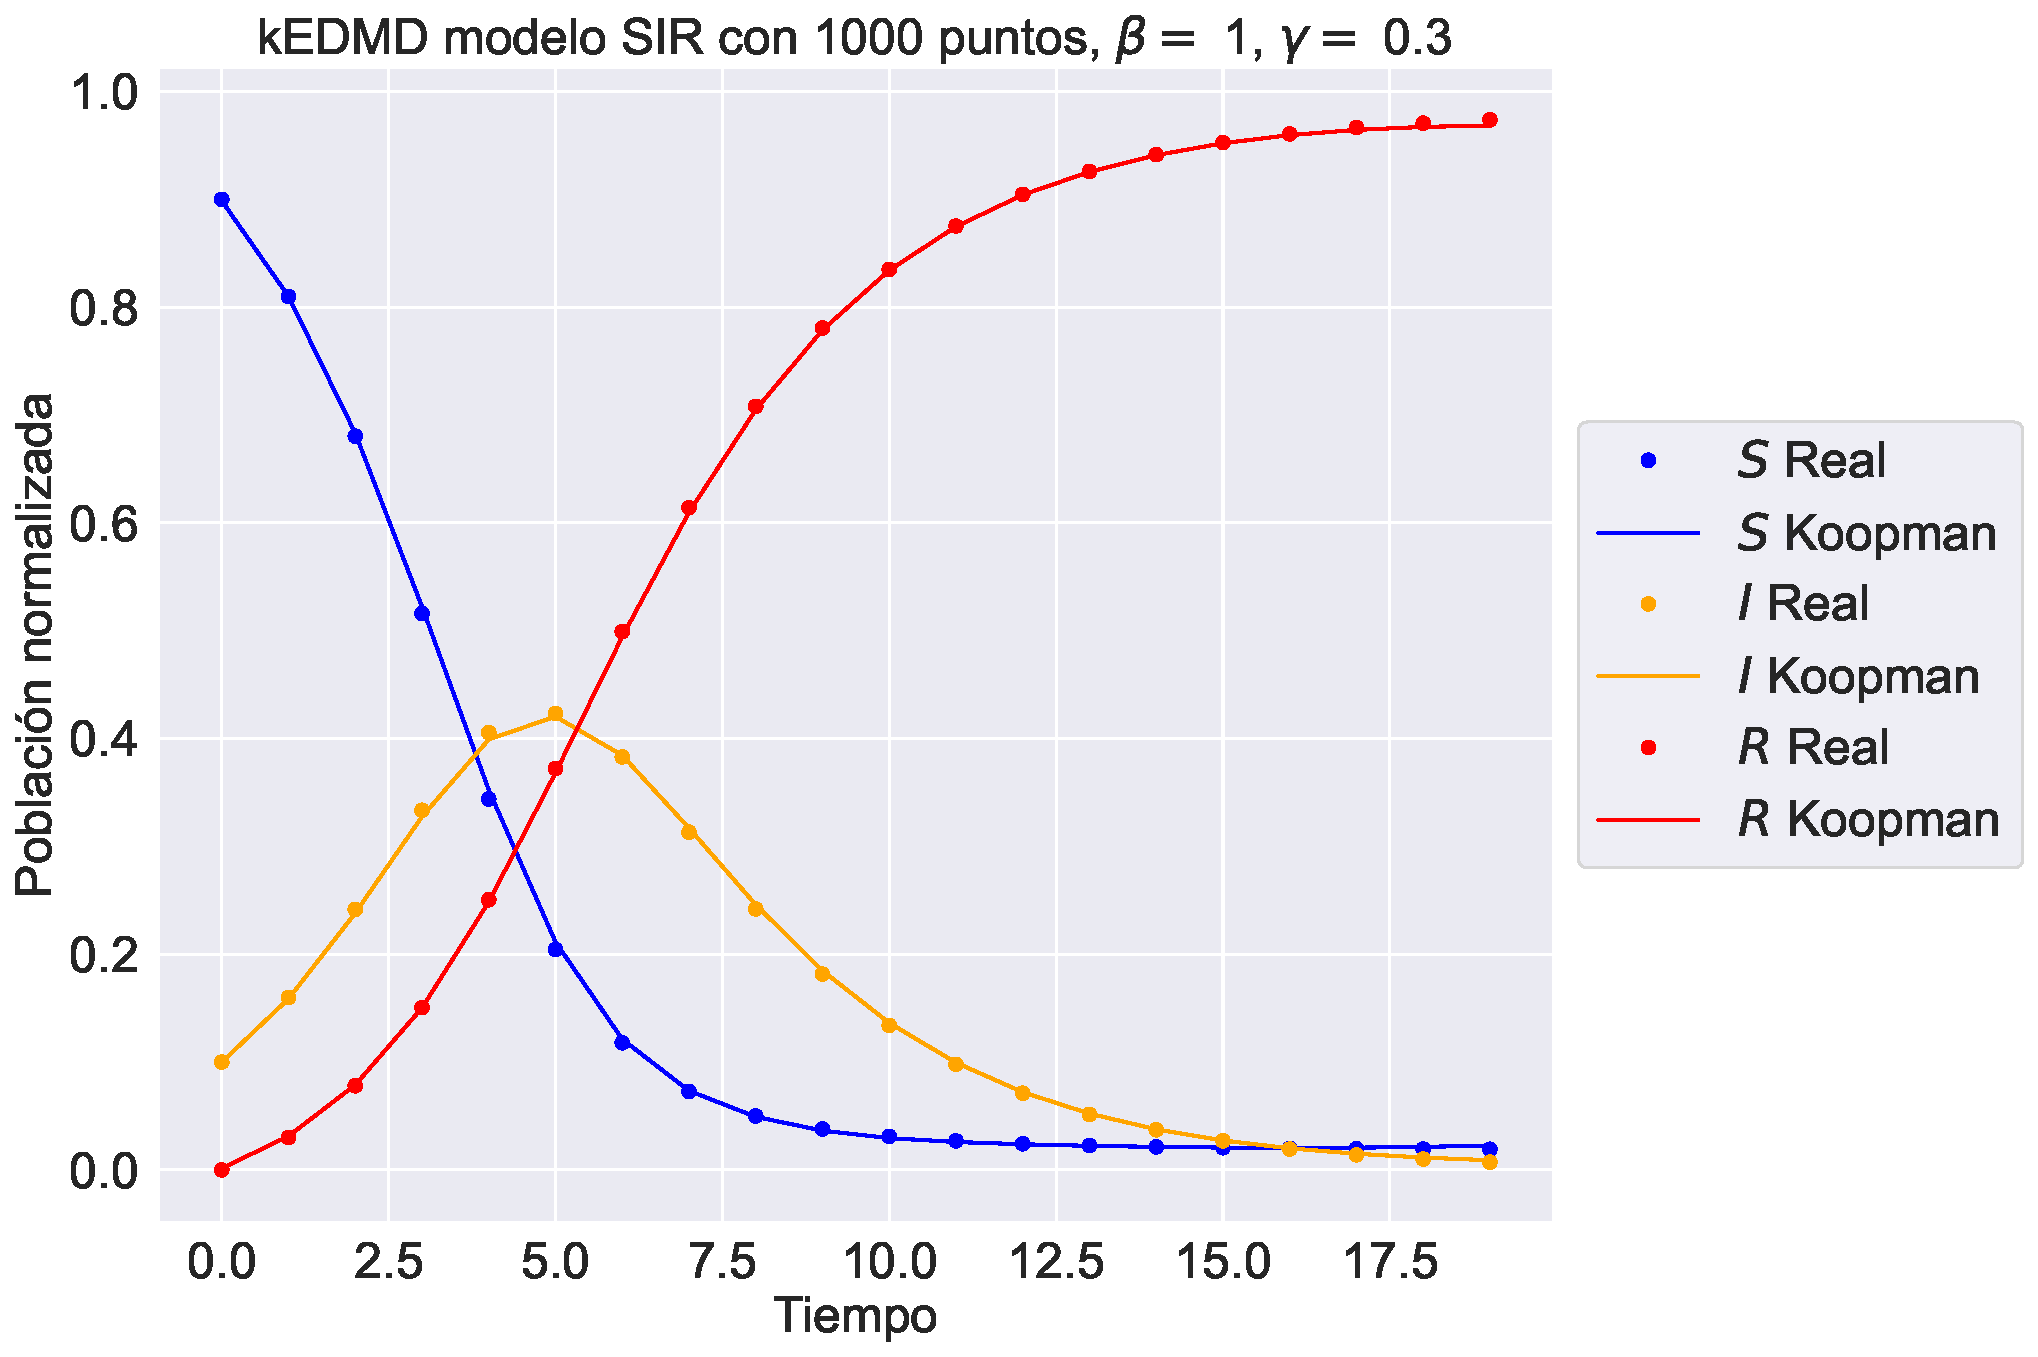
\includegraphics[width=\textwidth]{img/content/chapter3/SIR1.pdf}
        \caption{$\alpha=-0.3$}
        \label{fig:image1}
    \end{subfigure}
    \hfill
    \begin{subfigure}[b]{0.45\textwidth}
        \centering
        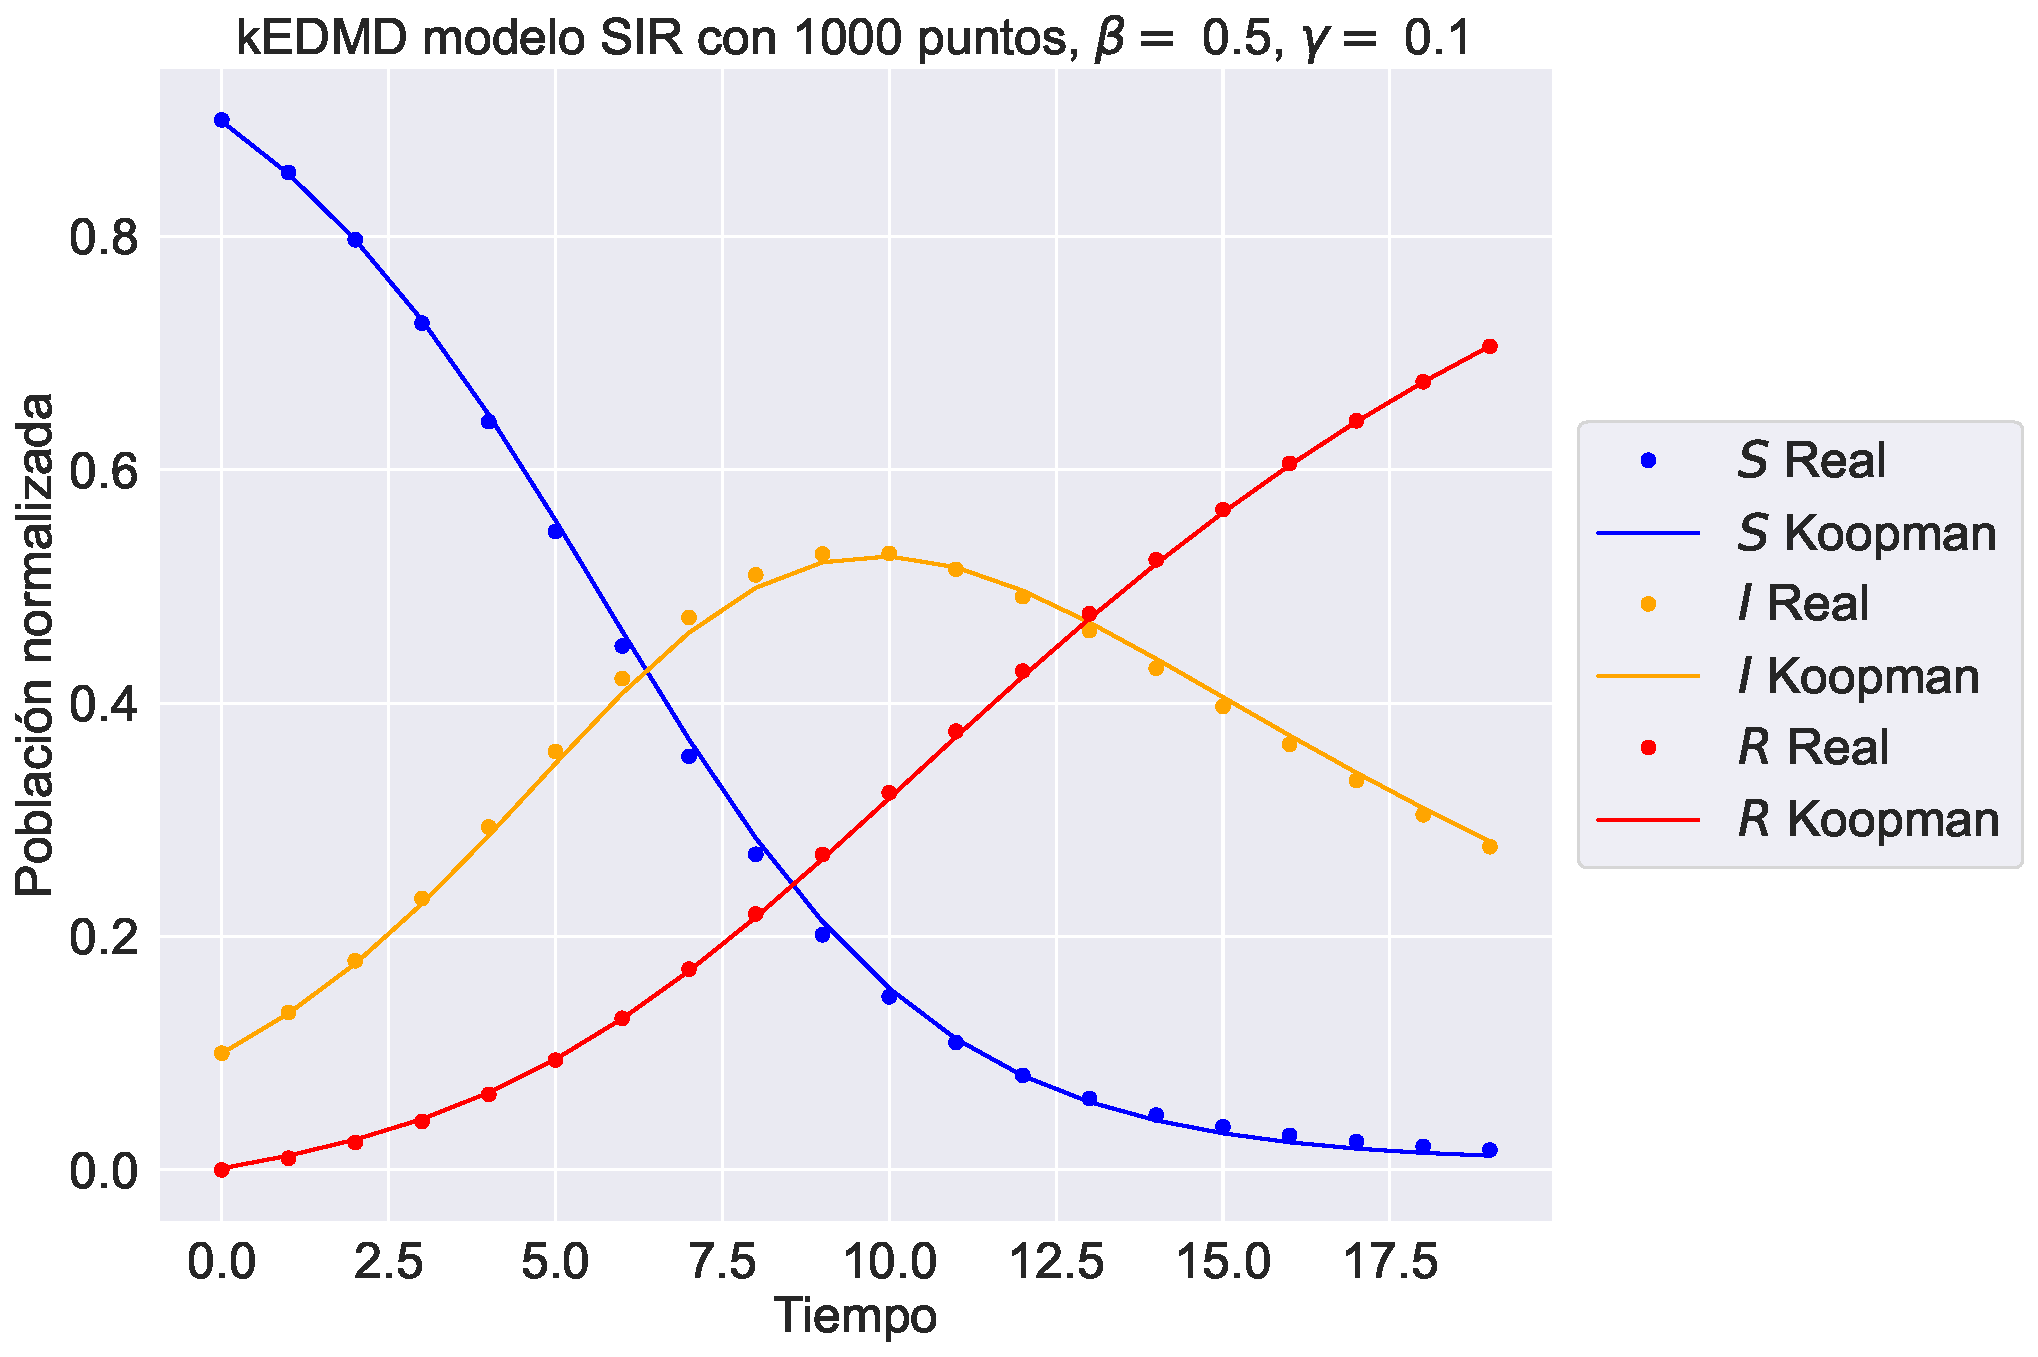
\includegraphics[width=\textwidth]{img/content/chapter3/SIR2.pdf}
        \caption{$\alpha=-0.1$}
        \label{fig:image2}
    \end{subfigure}
    \hfill
    \begin{subfigure}[b]{0.45\textwidth}
        \centering
        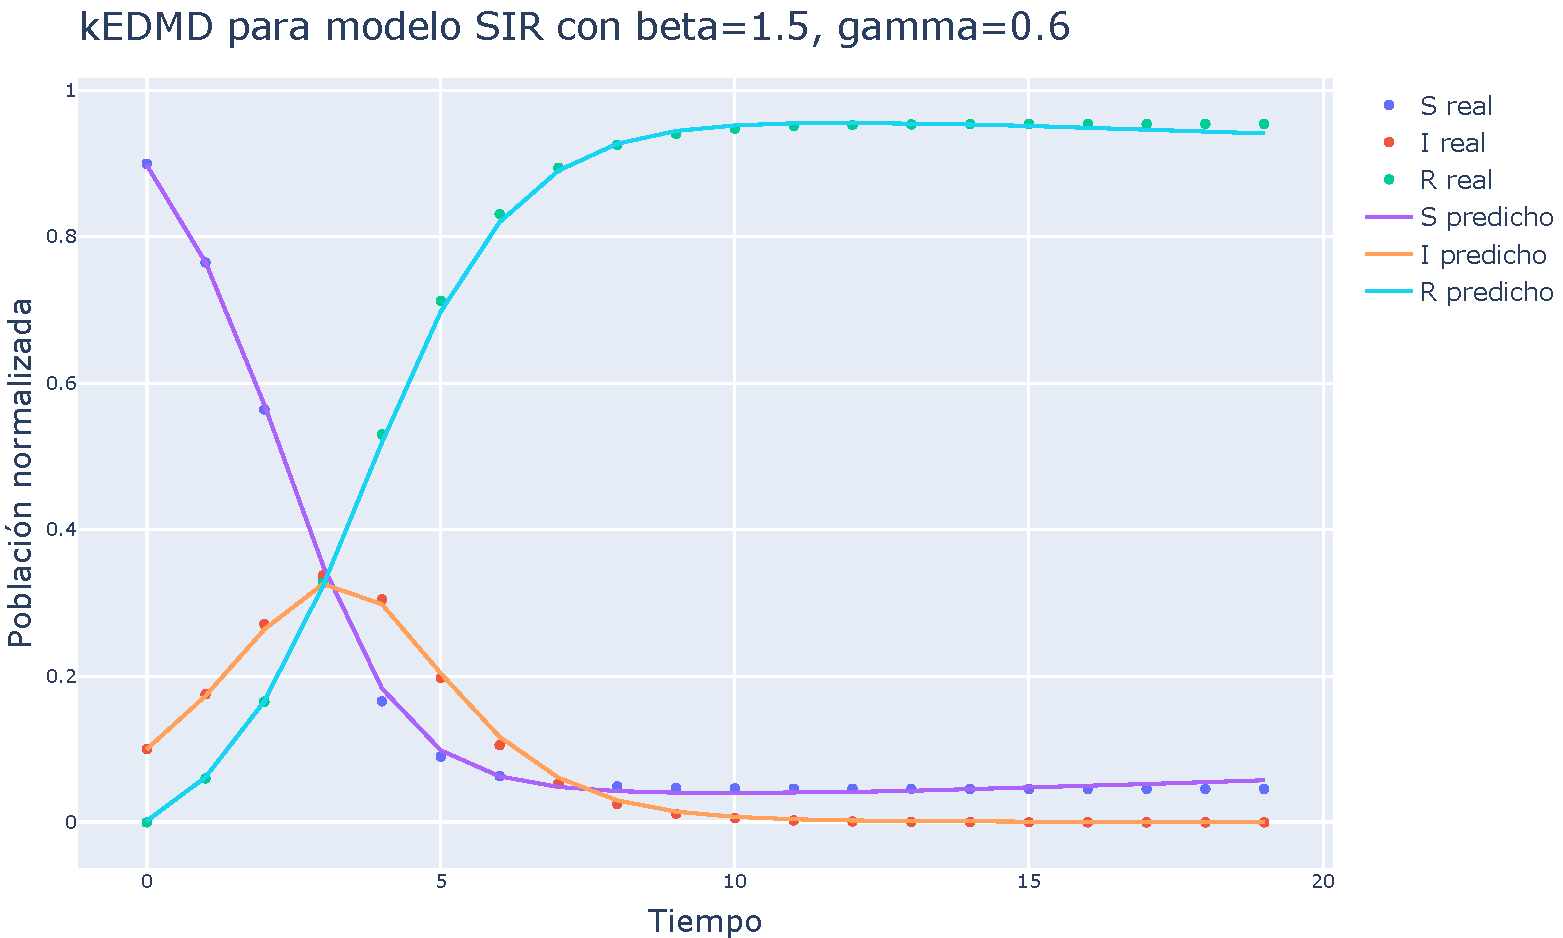
\includegraphics[width=\textwidth]{img/content/chapter3/SIR3.pdf}
        \caption{$\alpha=0.05$}
    \end{subfigure}
    \caption{Ilustración de los tres casos de $\beta$ y $\gamma$ elegidos para la comparación entre el sistema no lineal original y el sistema linealizado por Koopman a 1000 puntos \textit{sampleados} de una variable aleatoria Dirichlet. En forma de puntos se dejan los valores reales que toma el sistema y en línea continua los valores entregados por el sistema linealizado, que se consideran como predicción.}
    \label{fig:Comp_traj_SIR}
\end{figure}

\begin{figure}[h]
    \centering
    \begin{subfigure}[b]{0.32\textwidth}
        \centering
        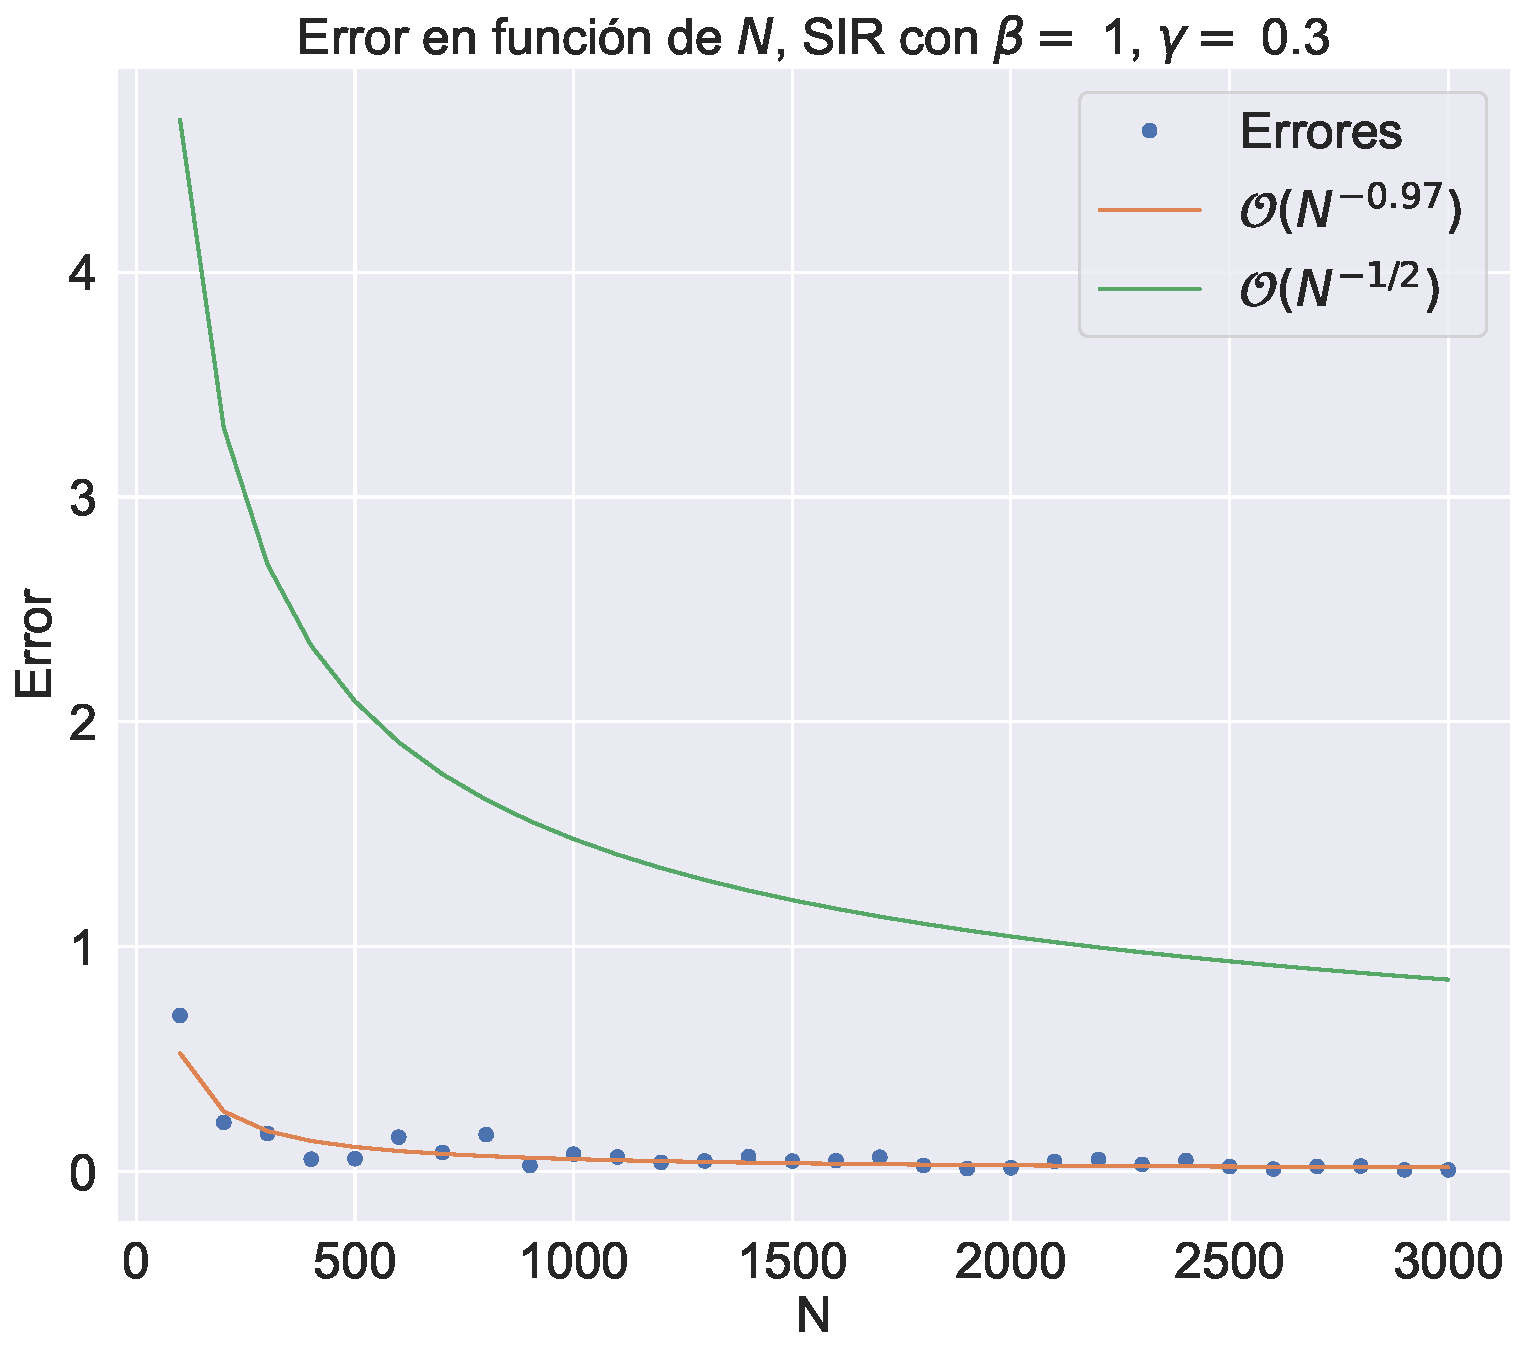
\includegraphics[width=\textwidth]{img/content/chapter3/SIR1Errors.pdf}
        \caption{$\beta=-0.3$, $\gamma=0.3$}
    \end{subfigure}
    \hfill
    \begin{subfigure}[b]{0.32\textwidth}
        \centering
        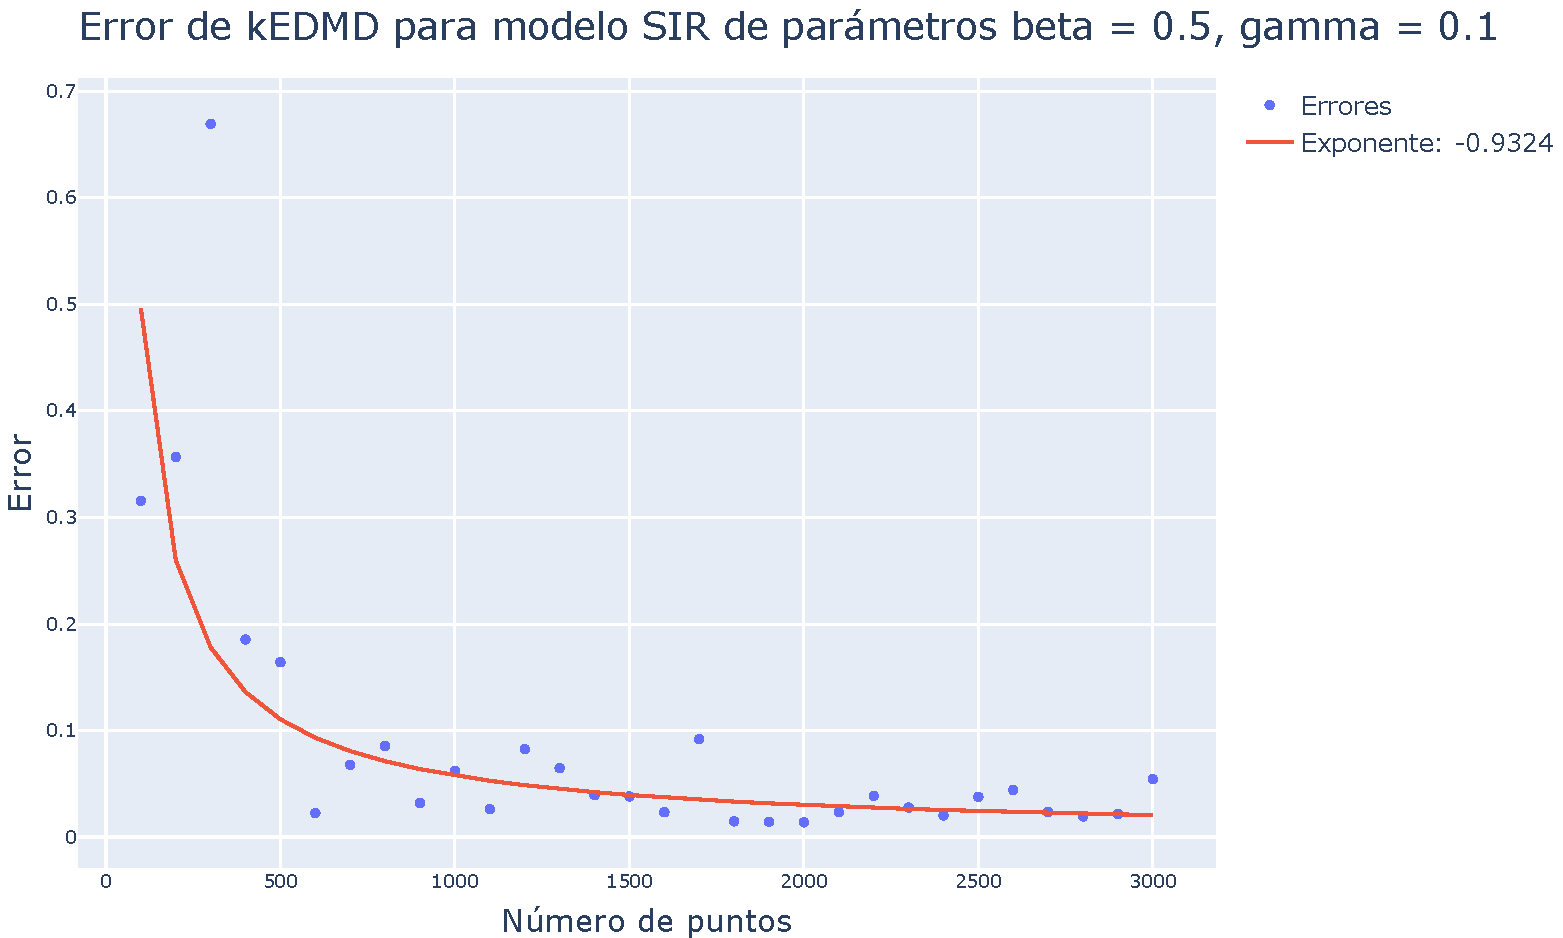
\includegraphics[width=\textwidth]{img/content/chapter3/SIR2Errors.pdf}
        \caption{$\beta=0.5$, $\gamma=0.1$}
    \end{subfigure}
    \hfill
    \begin{subfigure}[b]{0.32\textwidth}
        \centering
        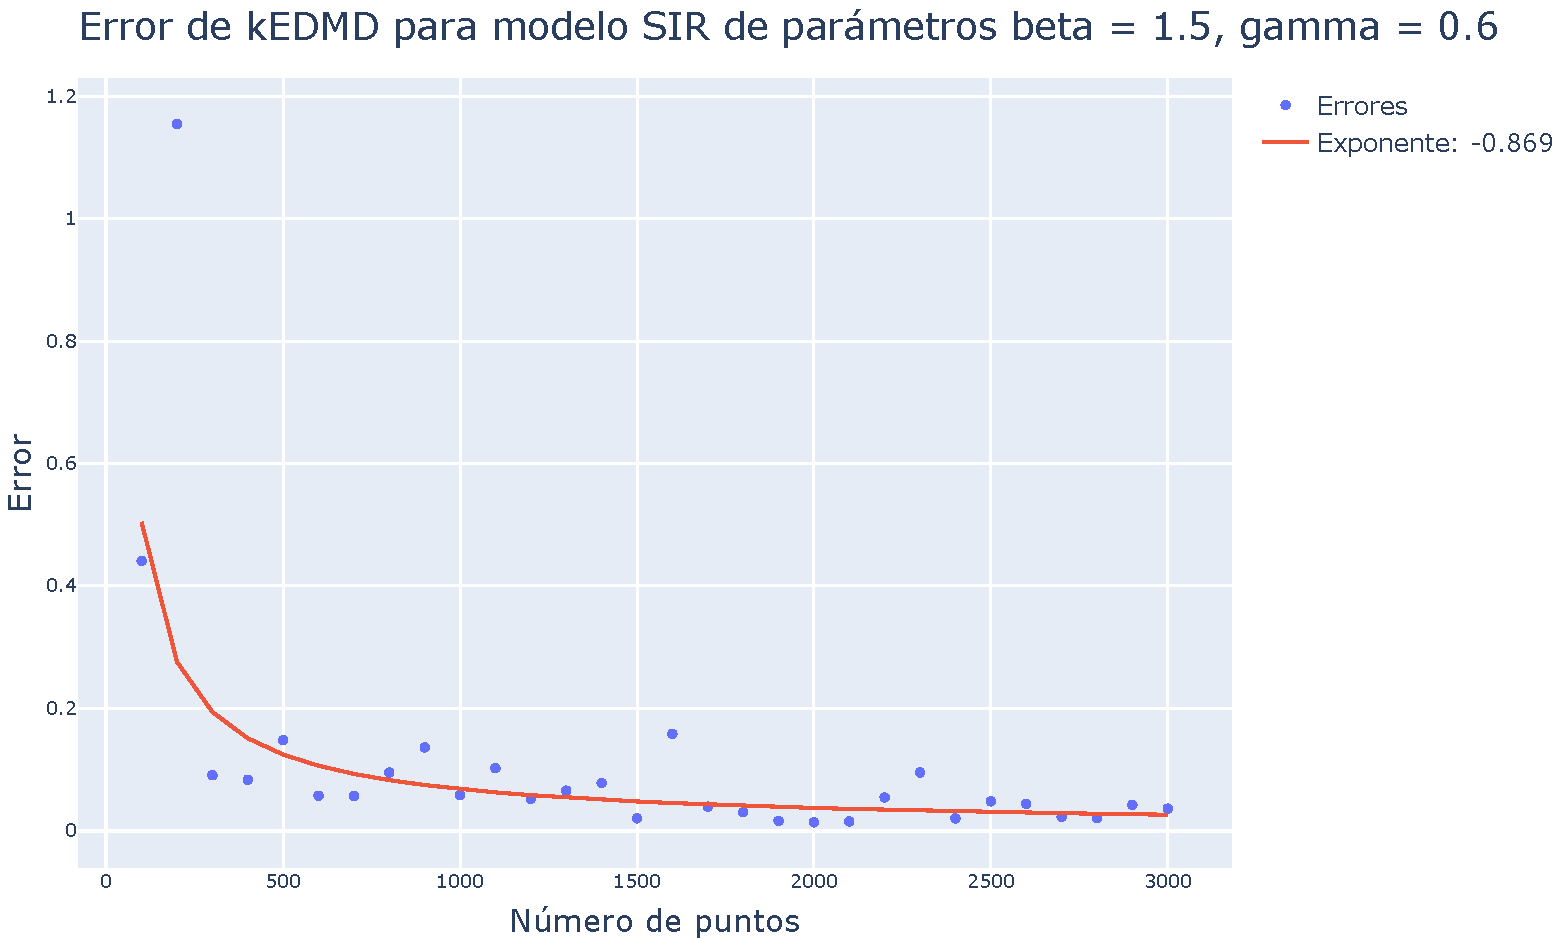
\includegraphics[width=\textwidth]{img/content/chapter3/SIR3Errors.pdf}
        \caption{$\beta=1.5$, $\gamma=0.6$}
    \end{subfigure}
    \caption{Ilustración de los tres casos del modelo SIR elegido para la evolución en función de $N$ de la diferencia en norma entre el sistema lineal original y el sistema linealizado por Koopman a $N$ puntos,  \textit{sampleados} de una variable aleatoria normal. En forma de puntos se deja la evolución observada del error y en línea continua la mejor curva de la forma $C \cdot N^{a}$, donde $a$ es el exponente que se deja en la leyenda.}
    \label{fig:ErrorSIR}
\end{figure}

\begin{figure}[h]
    \centering
    \begin{subfigure}[b]{0.45\textwidth}
        \centering
        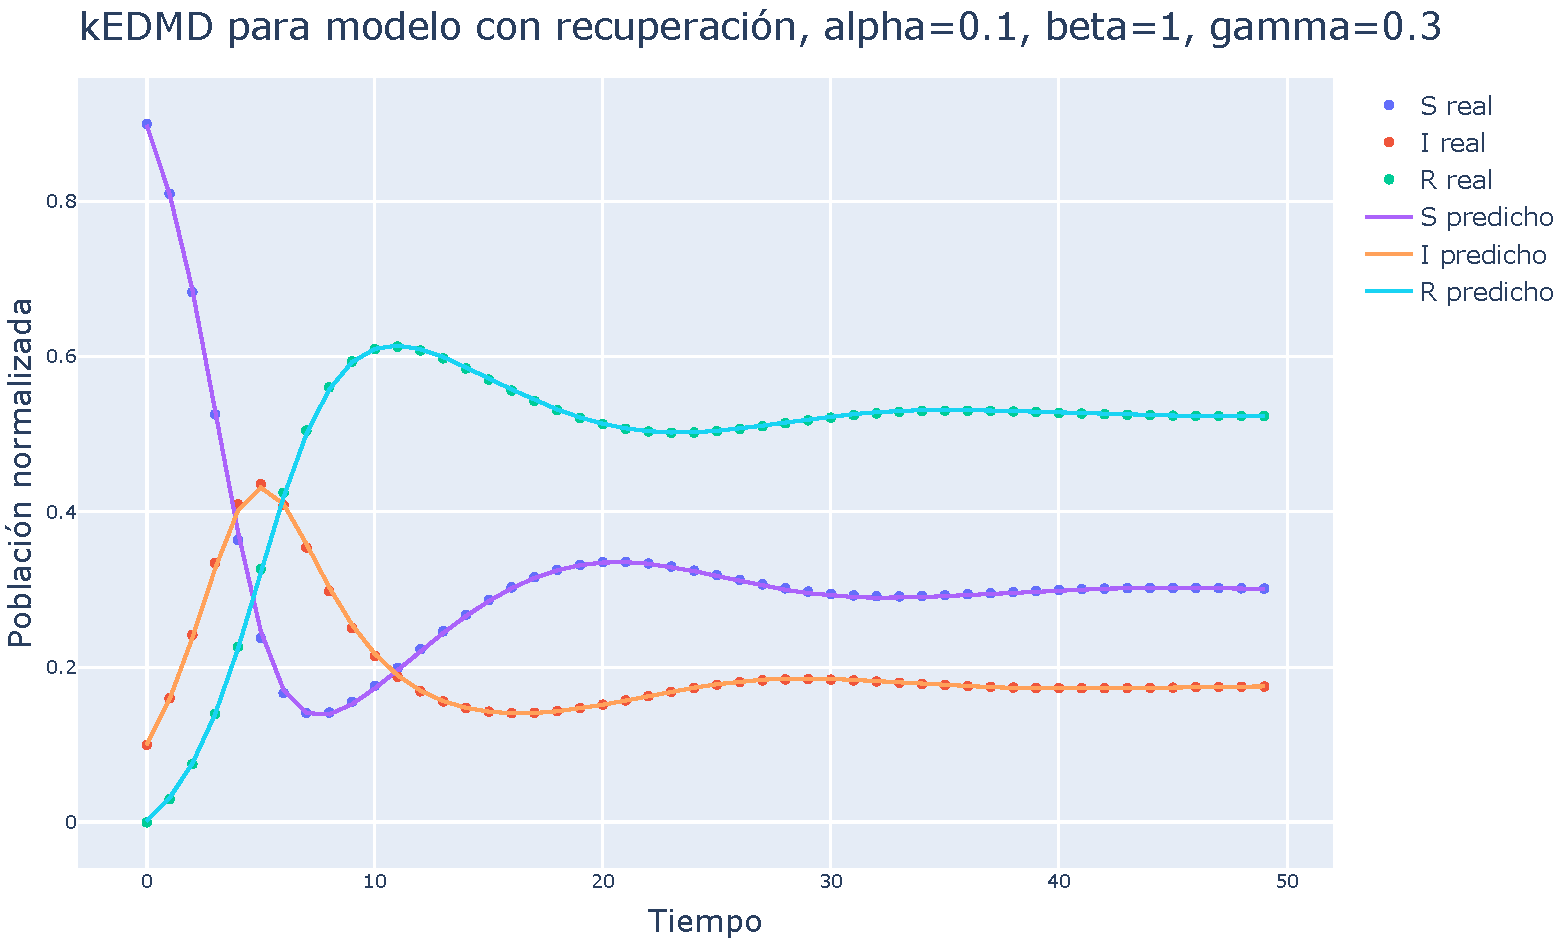
\includegraphics[width=\textwidth]{img/content/chapter3/SIR_rec1.pdf}
        \caption{$\alpha=-0.3$}
        \label{fig:image1}
    \end{subfigure}
    \hfill
    \begin{subfigure}[b]{0.45\textwidth}
        \centering
        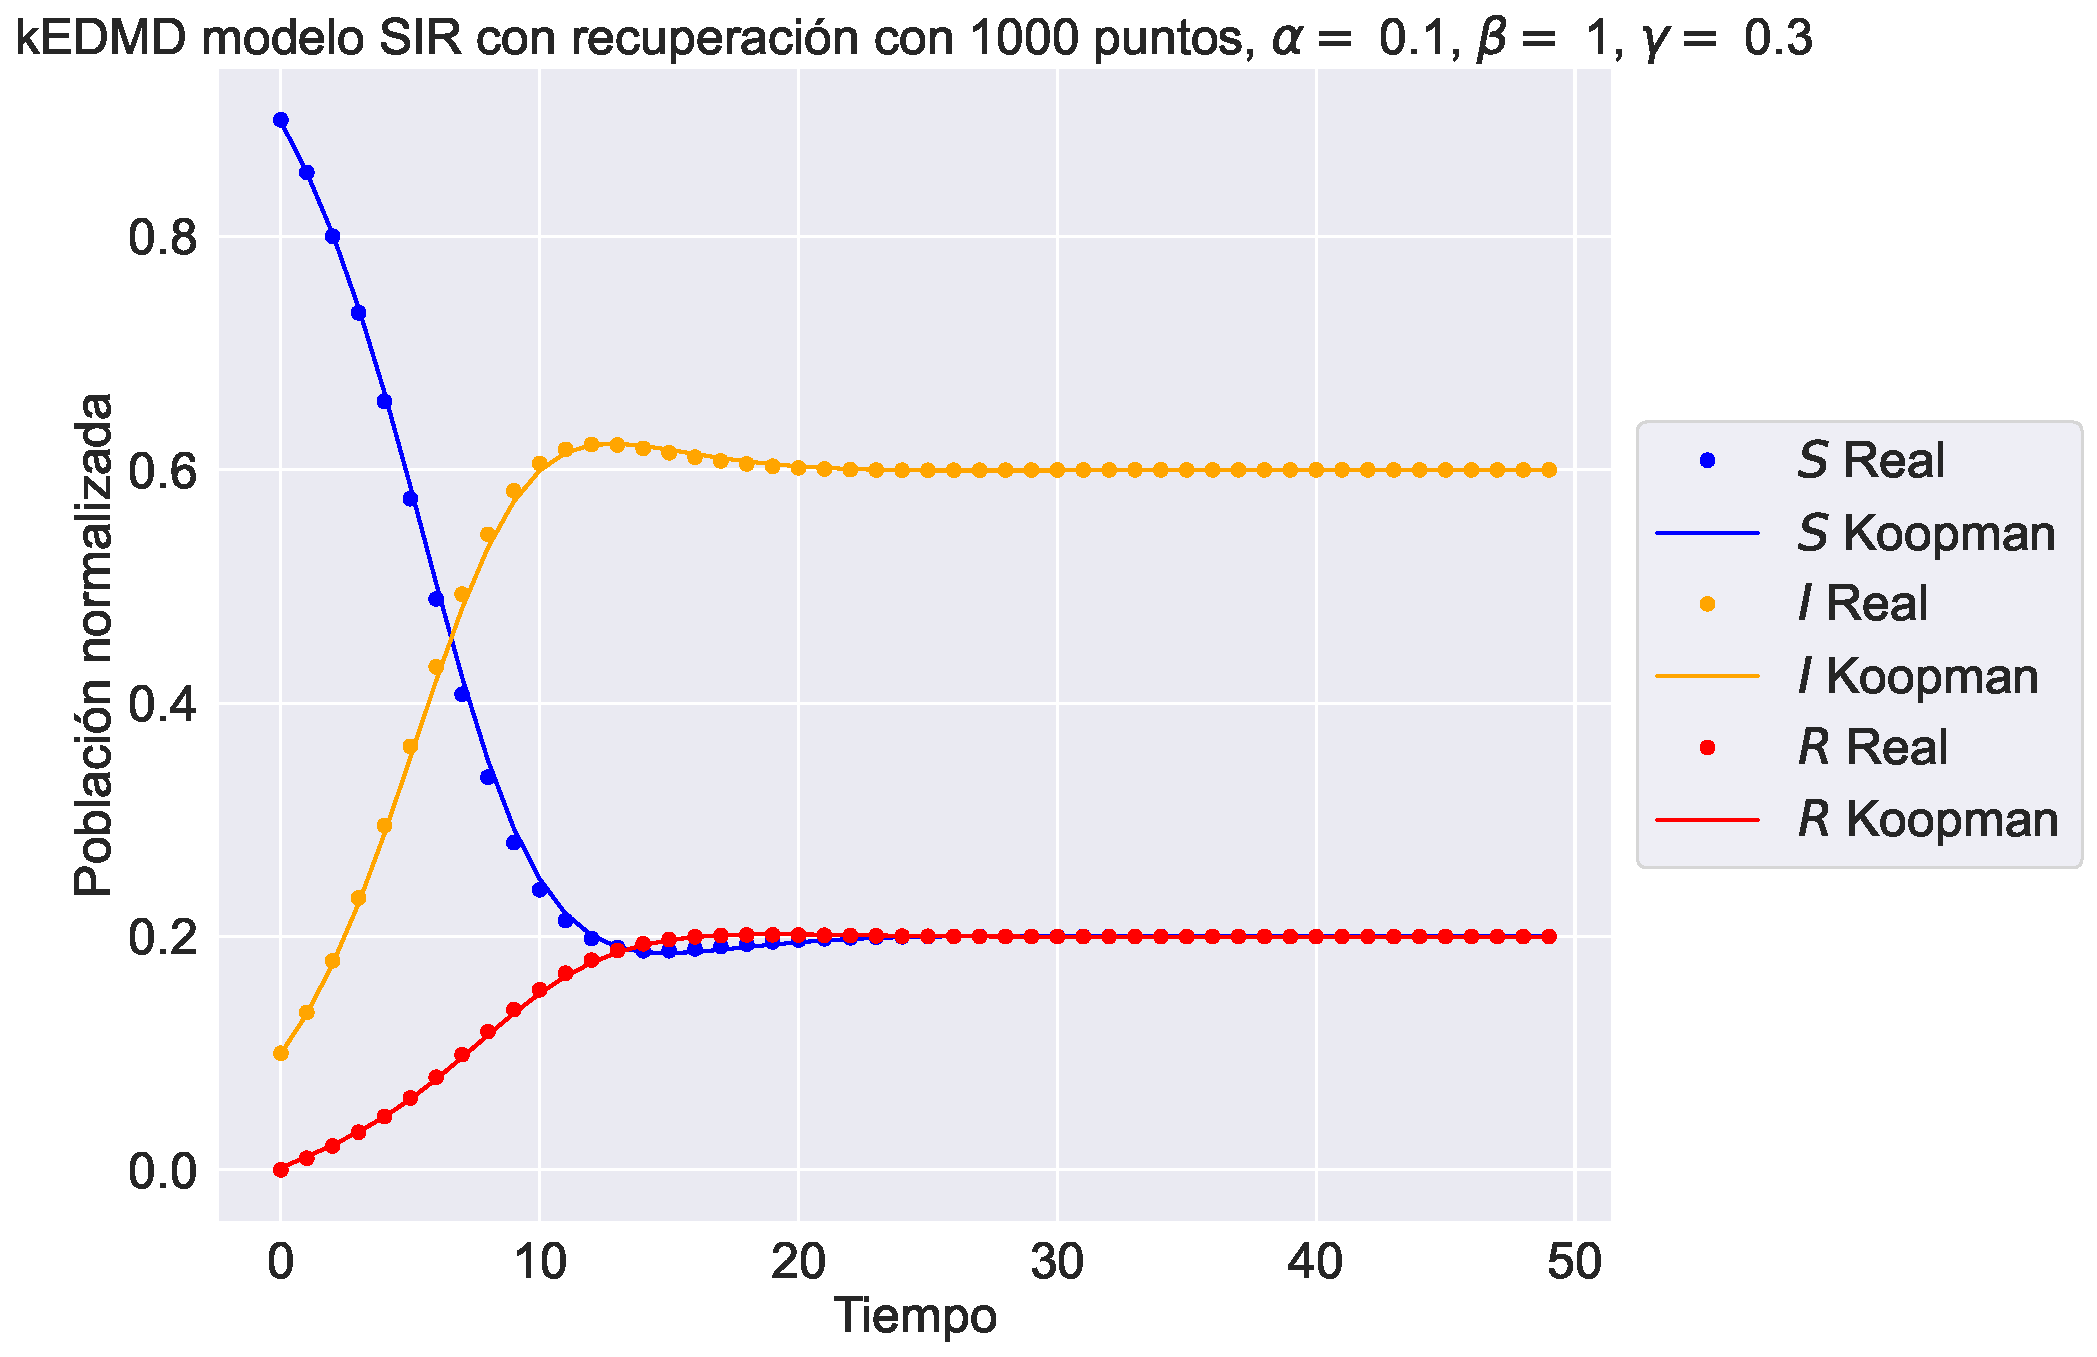
\includegraphics[width=\textwidth]{img/content/chapter3/SIR_rec2.pdf}
        \caption{$\alpha=-0.1$}
        \label{fig:image2}
    \end{subfigure}
    \hfill
    \begin{subfigure}[b]{0.45\textwidth}
        \centering
        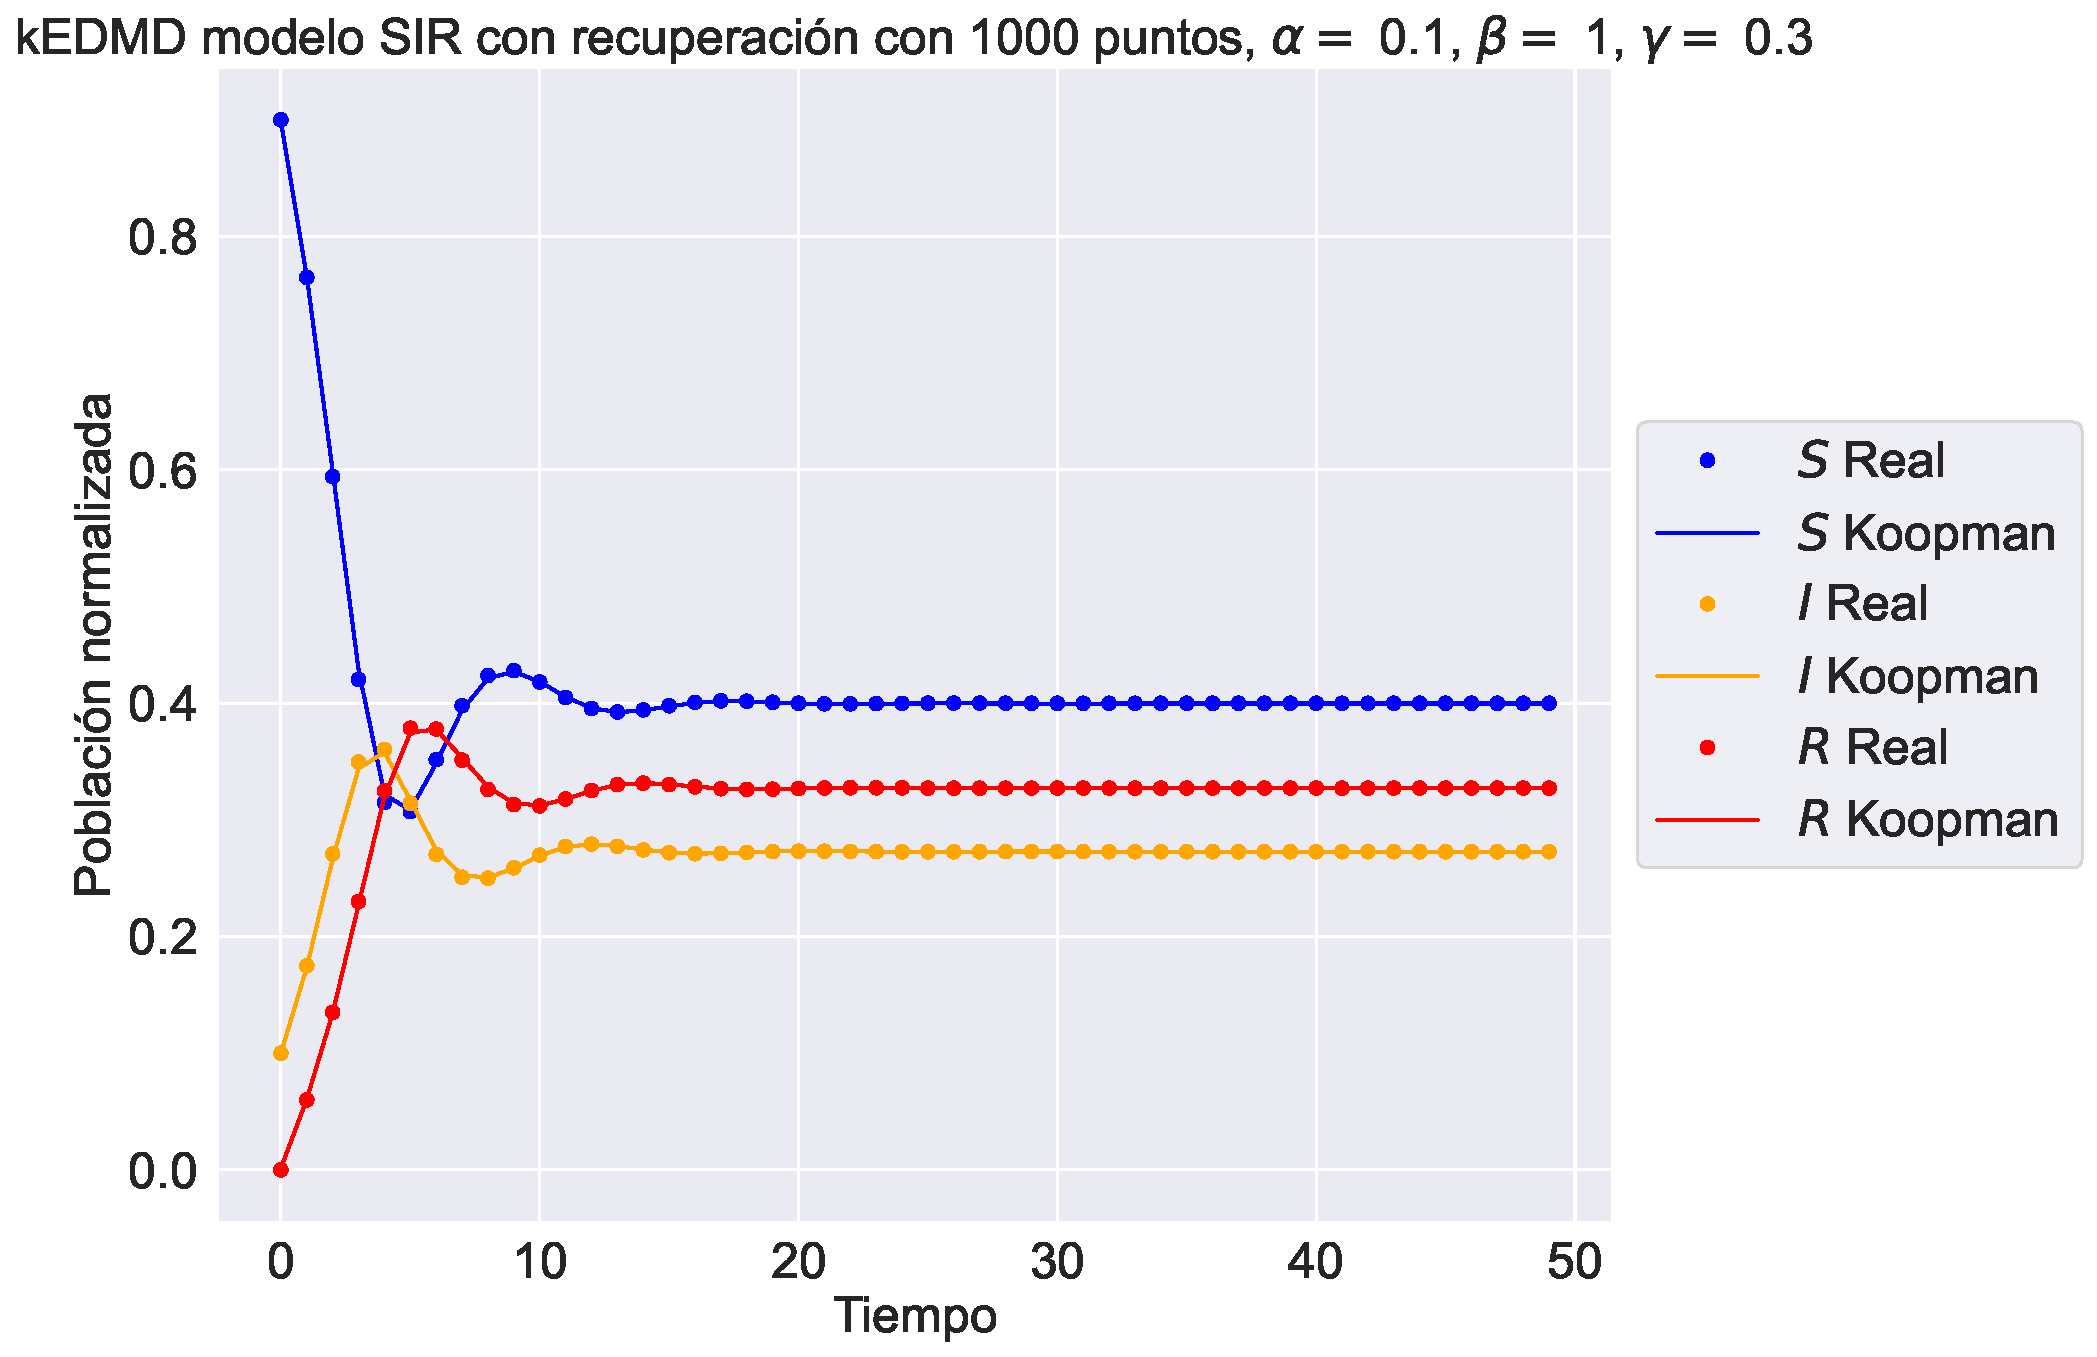
\includegraphics[width=\textwidth]{img/content/chapter3/SIR_rec3.pdf}
        \caption{$\alpha=0.05$}
    \end{subfigure}
    \caption{Ilustración de los tres casos de $\beta$ y $\gamma$ elegidos para la comparación entre el sistema no lineal original y el sistema linealizado por Koopman a 1000 puntos \textit{sampleados} de una variable aleatoria Dirichlet. En forma de puntos se dejan los valores reales que toma el sistema y en línea continua los valores entregados por el sistema linealizado, que se consideran como predicción.}
    \label{fig:Comp_traj_SIR}
\end{figure}
\begin{figure}[h]
    \centering
    \begin{subfigure}[b]{0.32\textwidth}
        \centering
        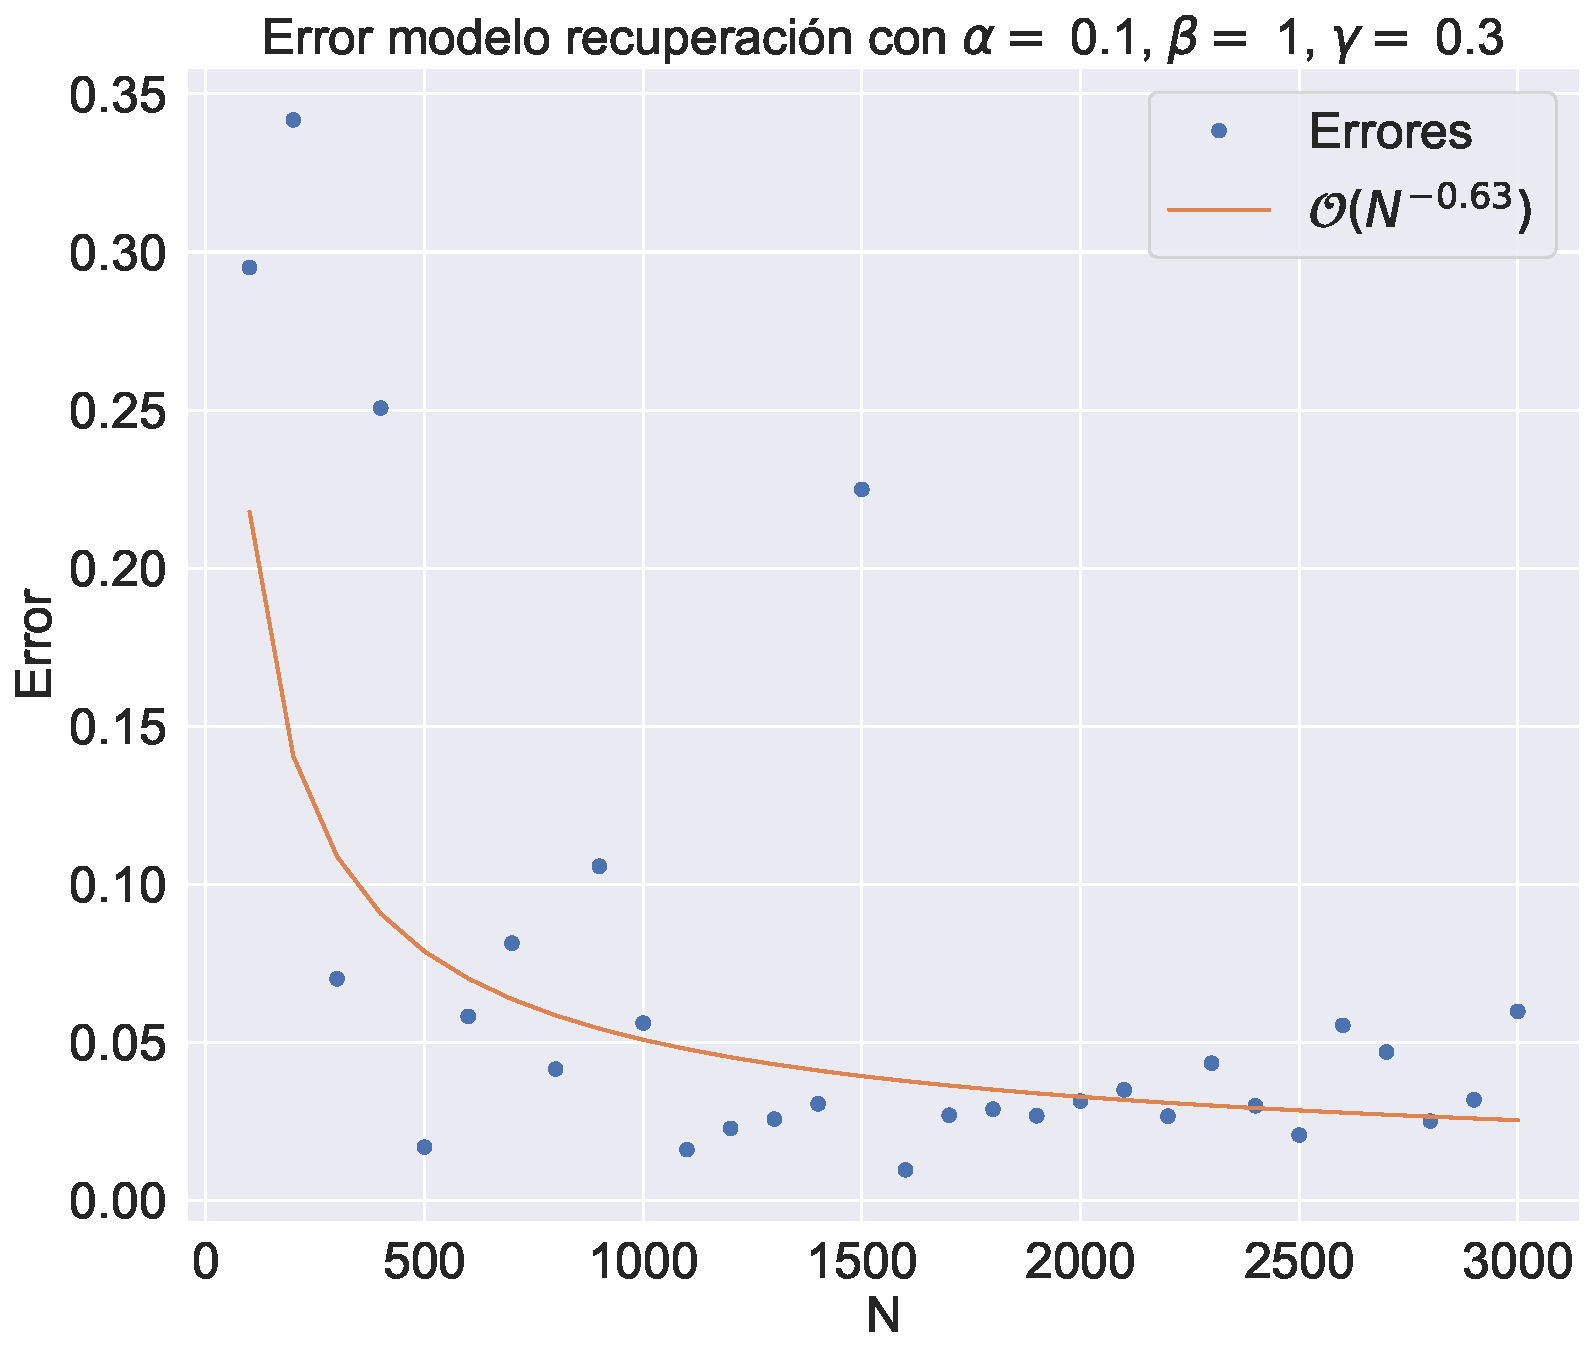
\includegraphics[width=\textwidth]{img/content/chapter3/SIR_rec1Errors.pdf}
        \caption{$\alpha=0.1$, $\beta=1$, $\gamma=0.3$}
    \end{subfigure}
    \hfill
    \begin{subfigure}[b]{0.32\textwidth}
        \centering
        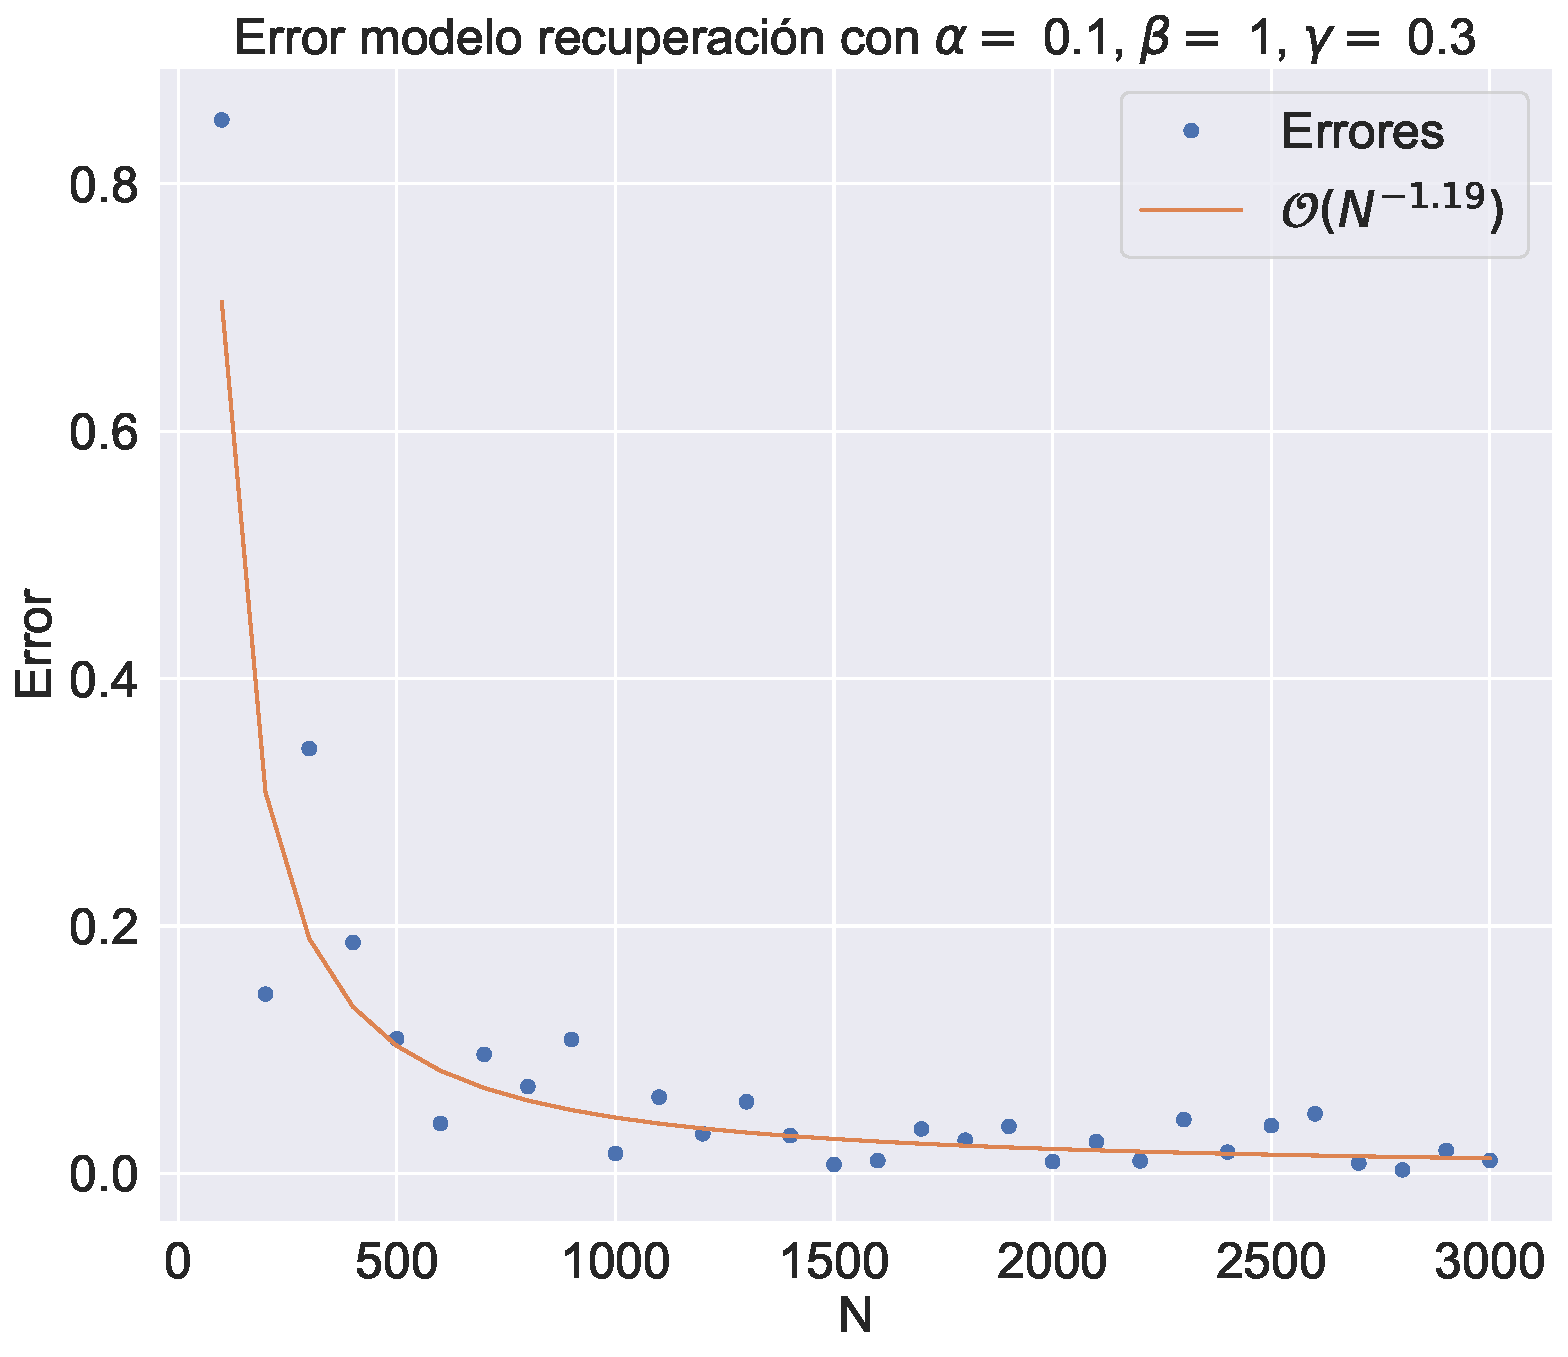
\includegraphics[width=\textwidth]{img/content/chapter3/SIR_rec2Errors.pdf}
        \caption{$\alpha=0.3$, $\beta=1$, $\gamma=0.3$}
    \end{subfigure}
    \hfill
    \begin{subfigure}[b]{0.32\textwidth}
        \centering
        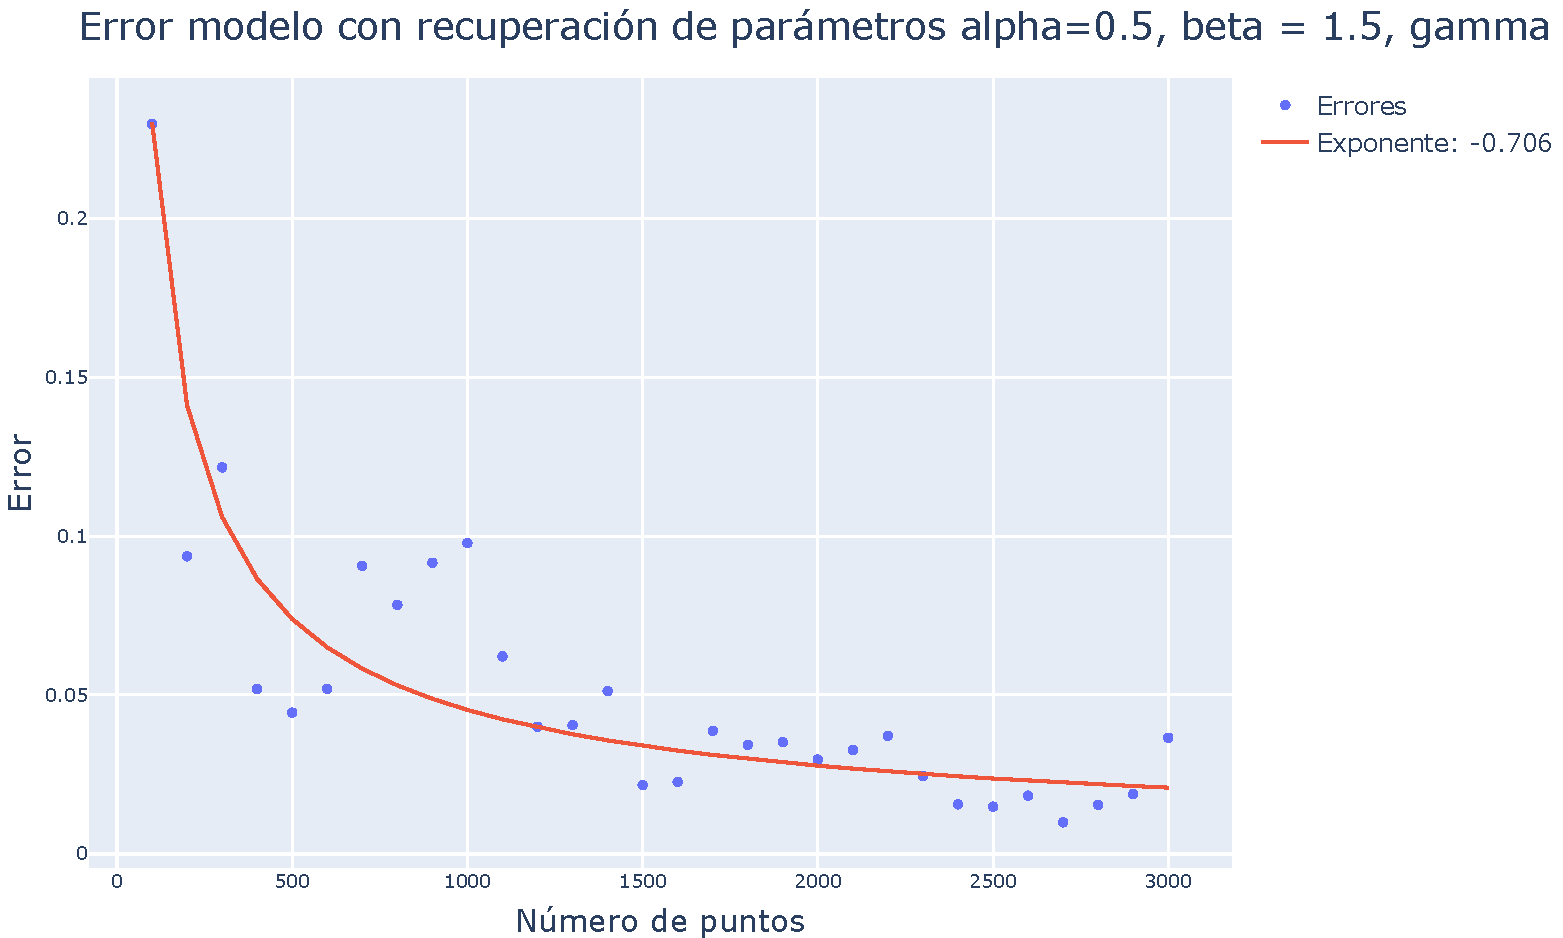
\includegraphics[width=\textwidth]{img/content/chapter3/SIR_rec3Errors.pdf}
        \caption{$\alpha=0.05$}
    \end{subfigure}
    \caption{Ilustración de los tres casos del modelo SIR con pérdida de inmunidad elegido para la evolución en función de $N$ de la diferencia en norma entre el sistema lineal original y el sistema linealizado por Koopman a $N$ puntos,  \textit{sampleados} de una variable aleatoria normal. En forma de puntos se deja la evolución observada del error y en línea continua la mejor curva de la forma $C \cdot N^{a}$, donde $a$ es el exponente que se deja en la leyenda.}
    \label{fig:ErrorSIR_rec}
\end{figure}


\chapter{Resultados numéricos capítulo 4}

\section{Comparación con el Filtro de Kalman}

\begin{figure}[h!]
    \centering
    \begin{subfigure}[b]{0.49\textwidth}
        \centering
        \includegraphics[width=0.75\linewidth]{img/content/chapter4/kalman_vs_kerKKF_01.pdf}
    \caption{$\alpha = -0.1$.}
    \label{fig:kalman_vs_kerKKF_01}
    \end{subfigure}
    \begin{subfigure}[b]{0.49\textwidth}
        \centering \includegraphics[width=0.75\linewidth]{img/content/chapter4/kalman_vs_kerKKF_001.pdf}
    \caption{$\alpha = 0.01$.}
    \label{fig:kalman_vs_kerKKF_001}
    \end{subfigure}
    \begin{subfigure}[b]{0.49\textwidth}
        \centering \includegraphics[width=0.75\linewidth]{img/content/chapter4/kalman_vs_kerKKF_025.pdf}
    \caption{$\alpha = -0.25$.}
    \label{fig:kalman_vs_kerKKF_025}
    \end{subfigure}
    \caption{Comparación de Kalman con kerKKF para distintos valores de $\alpha$. En azul el resultado del sistema simulado sin ruidos ni de dinámica ni observación, en naranja la solución del filtro de Kalman y en verde la de kerKKF.}
\end{figure}

\section{Comparación con otros filtros para modelos epidemiológicos}

\begin{figure}[h!]
    \centering
    \begin{subfigure}[b]{0.49\textwidth}
        \includegraphics[width=\linewidth]{img/content/chapter4/nonlinear_filters_sir_beta_06.pdf}
    \caption{$\beta = 0.6$.}
    \label{fig:nonlinear_filters_sir_beta_06}
    \end{subfigure}
    \begin{subfigure}[b]{0.49\textwidth}
        \includegraphics[width=\linewidth]{img/content/chapter4/nonlinear_filters_sir_beta_09.pdf}
    \caption{$\beta = 0.9$.}
    \label{fig:nonlinear_filters_sir_beta_09}
    \end{subfigure}
    \begin{subfigure}[b]{0.49\textwidth}
        \includegraphics[width=\linewidth]{img/content/chapter4/nonlinear_filters_sir_beta_15.pdf}
    \caption{$\beta = 1.5$.}
    \label{fig:nonlinear_filters_sir_beta_15}
    \end{subfigure}
    \caption{Comparación de resultados de las trayectorias generadas por los filtros EKF (naranja), UKF (verde), PF (rojo) y kerKKF (púrpura), junto con la trayectoria real (puntos azules) sin ruidos, ni de dinámica ni de observación, esto para cada uno de los estados del modelo SIR. $\beta$ varía en cada caso para (a), (b) y (c), mientras que $\gamma = 0.3$ y $\sigma = 0.01$ fijos.}
\end{figure}

\begin{table}[h!]
    \caption{Errores para distintos valores de $\beta$, parámetro que representa la no linealidad del sistema. Esto para $\gamma = 0.3$ y $\sigma = 0.01$ fijos.}
    \begin{subtable}{\linewidth}
        \centering
    \caption{Errores para $\beta = 0.6$ y $\gamma = 0.3$}
    \begin{tabular}{|c|c|c|c|c|}
    \hline
    \textbf{Estado} & \textbf{EKF} & \textbf{UKF} & \textbf{PF} & \textbf{kerKKF} \\ \hline
    S & 0.2442 & 0.2379 & 0.3305 & 0.1629 \\ \hline
    I & 0.2904 & 0.2815 & 0.2903 & 0.1352 \\ \hline
    R & 0.4874 & 0.5503 & 0.4732 & 0.1210 \\ \hline
    \end{tabular}
    \label{tab:errores_beta_gamma_06}
    \end{subtable}
    \begin{subtable}{\linewidth}
        \centering
    \caption{Errores para $\beta = 0.9$ y $\gamma = 0.3$}
    \begin{tabular}{|c|c|c|c|c|}
    \hline
    \textbf{Estado} & \textbf{EKF} & \textbf{UKF} & \textbf{PF} & \textbf{kerKKF} \\ \hline
    S & 0.1486 & 0.1533 & 0.2195 & 0.1672 \\ \hline
    I & 0.2808 & 0.2590 & 0.2798 & 0.1628 \\ \hline
    R & 0.4866 & 0.5246 & 0.4907 & 0.1300 \\ \hline
    \end{tabular}
    \label{tab:errores_beta_gamma_09}
    \end{subtable}
    \begin{subtable}{\linewidth}
        \centering
    \caption{Errores para $\beta = 1.5$ y $\gamma = 0.3$}
    \begin{tabular}{|c|c|c|c|c|}
    \hline
    \textbf{Estado} & \textbf{EKF} & \textbf{UKF} & \textbf{PF} & \textbf{kerKKF} \\ \hline
    S & 0.0885 & 0.2296 & 0.2292 & 0.1906 \\ \hline
    I & 0.2834 & 0.2788 & 0.2816 & 0.1934 \\ \hline
    R & 0.4671 & 0.5295 & 0.4042 & 0.1435 \\ \hline
    \end{tabular}
    \label{tab:errores_beta_gamma_15}
    \end{subtable}
\end{table}

\begin{figure}[h!]
    \centering
    \includegraphics[width=0.9\linewidth]{img/content/chapter4/nonlinear_filters_sir_error_beta.pdf}
    \caption{Error en norma de EKF (azul), UKF (naranja), PF (verde) y kerKKF (rojo) para distintos valores de $\beta$ entre $0.1$ y $2.5$. Eje y en escala logarítmica.}
    \label{fig:nonlinear_filters_sir_error_beta}
\end{figure}

\newpage

\section{Comparación con métodos de Markov Chain Monte Carlo}


\begin{figure}[h!]
    \centering
    \begin{subfigure}[b]{0.49\textwidth}
    \centering
         \includegraphics[width=0.8\linewidth]{img/content/chapter4/nonlinear_filters_sir_params.pdf}
    \caption{}
    \end{subfigure}
   \begin{subfigure}[b]{0.49\textwidth}
   \centering
       \includegraphics[width=0.8\linewidth]{img/content/chapter4/nonlinear_filters_sir_params_evolution.pdf}
       \caption{}
   \end{subfigure}
    \caption{Resultado para modelo SIR \eqref{eq:SIR}. \\
    (a) Resultado de kerKKF para estimación de parámetros, primera cadena. \\
    (b) Evolución de la estimación de los parámetros a través de las iteraciones del algoritmo de estimación, primera cadena. De color rojo, el régimen de \textit{warm up}, mientras que en naranja se encuentran que sí serán consideradas para la estimación. En azul se encuentra el valor real del parámetro.}
    \label{fig:param_estim_SIR}
\end{figure}

\begin{figure}[h!]
    \centering
    \begin{subfigure}[b]{0.8\textwidth}
        \centering\includegraphics[width=0.8\linewidth]{img/content/chapter4/nonlinear_filters_sir_params_density.pdf}
    \caption{Densidades de las 8 cadenas.}
    \label{fig:nonlinear_filters_sir_params_density}
    \end{subfigure}
        
    \begin{subfigure}[b]{0.8\textwidth}
        \centering \includegraphics[width=0.8\linewidth]{img/content/chapter4/nonlinear_filters_sir_params_density_mean.pdf}
    \caption{Densidad promedio entre las 8 cadenas.}
    \label{fig:nonlinear_filters_sir_params_density_mean}
    \end{subfigure}
    \caption{Densidades de estimación para los parámetros del modelo SIR.}
\end{figure}

\begin{figure}[h!]
    \centering
    \begin{subfigure}[b]{0.49\textwidth}
         \centering
         \includegraphics[height=0.9\linewidth]{img/content/chapter4/nonlinear_filters_sir_rec_params.pdf}
         \caption{}
         \label{fig:nonlinear_filters_sir_rec_params}
    \end{subfigure}
    \begin{subfigure}[b]{0.49\textwidth}
         \centering \includegraphics[height=0.9\linewidth]{img/content/chapter4/nonlinear_filters_sir_rec_params_evolution.pdf}
         \caption{}
         \label{fig:nonlinear_filters_sir_rec_params_evolution}
    \end{subfigure}
    \caption{Resultado para modelo SIR con pérdida de inmunidad \eqref{eq:SIR_rec}. \\
    (a) Resultado de kerKKF para estimación de parámetros, primera cadena. \\
    (b) Evolución de la estimación de los parámetros a través de las iteraciones del algoritmo de estimación, primera cadena. De color rojo, el régimen de \textit{warm up}, mientras que en naranja se encuentran que sí serán consideradas para la estimación. En azul se encuentra el valor real del parámetro.}
    \label{fig:SIR_inmun}
\end{figure}

\begin{figure}[h]
    \centering
    \begin{subfigure}[b]{0.8\textwidth}
        \centering \includegraphics[width=0.8\linewidth]{img/content/chapter4/nonlinear_filters_sir_rec_params_density.pdf}
    \caption{Densidades de las 8 cadenas.}
    \label{fig:nonlinear_filters_sir_rec_params_density}
    \end{subfigure}
    \begin{subfigure}[b]{0.8\textwidth}
        \centering \includegraphics[width=0.8\linewidth]{img/content/chapter4/nonlinear_filters_sir_rec_params_density_mean.pdf}
    \caption{Densidad promedio entre las 8 cadenas.}
    \label{fig:nonlinear_filters_sir_rec_params_density_mean}
    \end{subfigure}
    \caption{Densidades de estimación para los parámetros del modelo SIR con pérdida de inmunidad.}
\end{figure}

\begin{figure}[h]
    \centering
    \begin{subfigure}[b]{0.49\textwidth}
         \includegraphics[height=0.9\linewidth]{img/content/chapter4/nonlinear_filters_seir_params.pdf}
         \caption{}
         \label{fig:nonlinear_filters_sir_rec_params}
    \end{subfigure}
    \begin{subfigure}[b]{0.49\textwidth}
         \includegraphics[height=0.9\linewidth]{img/content/chapter4/nonlinear_filters_seir_params_evolution.pdf}
         \caption{}
         \label{fig:nonlinear_filters_seir_params_evolution}
    \end{subfigure}
    \caption{Resultado para modelo SEIR \eqref{eq:SEIR}. \\
    (a) Resultado de kerKKF para estimación de parámetros, primera cadena. \\
    (b) Evolución de la estimación de los parámetros a través de las iteraciones del algoritmo de estimación, primera cadena. De color rojo, el régimen de \textit{warm up}, mientras que en naranja se encuentran que sí serán consideradas para la estimación. En azul se encuentra el valor real del parámetro.}
    \label{fig:SEIR}
\end{figure}

\begin{figure}[h]
    \centering
    \begin{subfigure}[b]{0.8\textwidth}
        \centering \includegraphics[width=0.8\linewidth]{img/content/chapter4/nonlinear_filters_seir_params_density.pdf}
    \caption{Densidades de las 8 cadenas.}
    \label{fig:nonlinear_filters_sir_rec_params_density}
    \end{subfigure}
    \begin{subfigure}[b]{0.8\textwidth}
        \centering \includegraphics[width=0.8\linewidth]{img/content/chapter4/nonlinear_filters_seir_params_density_mean.pdf}
    \caption{Densidad promedio entre las 8 cadenas.}
    \label{fig:nonlinear_filters_seir_params_density_mean}
    \end{subfigure}
    \caption{Densidades de estimación para los parámetros del modelo SEIR.}
\end{figure}

\begin{figure}[h]
    \centering
    \begin{subfigure}[b]{0.49\linewidth}
        \centering \includegraphics[height=0.7\linewidth]{img/content/chapter4/DEMetropolis_sir_params_trace.pdf}
        \caption{DEMetropolisZ, 20000 iteraciones de estimación y 20000 de \textit{warm up}.}
        \label{fig:DEMetropolis_sir_rec_params_trace}
    \end{subfigure}
    \begin{subfigure}[b]{0.49\linewidth}
        \centering \includegraphics[height=0.7\linewidth]{img/content/chapter4/NUTS_sir_params_trace.pdf}
        \caption{NUTS, 150 iteraciones de estimación y 150 de \textit{warm up}.}
        \label{fig:NUTS_sir_params_trace}
    \end{subfigure}
    \caption{Evolución de los parámetros de SIR para una cadena de MCMC. Se muestran las iteraciones posteriores a las de \textit{warm up}, en naranjo el valor estimado del parámetro y en línea punteada el valor real.}
    \label{fig:MCMC_sir_params_trace}
\end{figure}

\begin{figure}[h]
    \centering
    \begin{subfigure}[b]{\linewidth}
        \centering
        \includegraphics[width=0.55\linewidth]{img/content/chapter4/DEMetropolis_sir_params_density.pdf}
        \caption{Densidad de las 8 cadenas.}
    \end{subfigure}
     \begin{subfigure}[b]{\linewidth}
        \centering
        \includegraphics[width=0.55\linewidth]{img/content/chapter4/DEMetropolis_sir_params_density_mean.pdf}
        \caption{Densidad de las 8 cadenas.}
    \end{subfigure}
    \caption{Densidad de los parámetros del modelo SIR estimados con MCMC con \textit{sampler} DEMEtropolisZ.}
\end{figure}

\begin{figure}[h]
    \centering
    \begin{subfigure}[b]{\linewidth}
        \centering
        \includegraphics[width=0.55\linewidth]{img/content/chapter4/NUTS_sir_params_density.pdf}
        \caption{Densidad de las 8 cadenas.}
    \end{subfigure}
     \begin{subfigure}[b]{\linewidth}
        \centering
        \includegraphics[width=0.55\linewidth]{img/content/chapter4/NUTS_sir_params_density_mean.pdf}
        \caption{Densidad de las 8 cadenas.}
    \end{subfigure}
    \caption{Densidad de los parámetros del modelo SIR estimados con MCMC con \textit{sampler} NUTS.}
\end{figure}

\begin{figure}[h]
    \centering
    \begin{subfigure}[b]{0.49\linewidth}
        \centering
        \includegraphics[width=\linewidth]{img/content/chapter4/DEMetropolis_sir_rec_params_trace.pdf}
        \caption{DEMetropolisZ, 20000 iteraciones de estimación y 20000 de \textit{warm up}.}
        \label{fig:NUTS_sir_rec_params_trace}
    \end{subfigure}
    \begin{subfigure}[b]{0.49\linewidth}
        \centering
        \includegraphics[width=\linewidth]{img/content/chapter4/NUTS_sir_rec_params_trace.pdf}
        \caption{NUTS, 150 iteraciones de estimación y 150 de \textit{warm up}.}
        \label{fig:NUTS_sir_rec_params_trace}
    \end{subfigure}
    \caption{Evolución de los parámetros de SIR con pérdida de inmunidad para una cadena de MCMC. Se muestran las iteraciones posteriores a las de \textit{warm up}, en naranjo el valor estimado del parámetro y en línea punteada el valor real.}
    \label{fig:MCMC_sir_params_trace}
\end{figure}

\begin{figure}[h]
    \centering
    \begin{subfigure}[b]{\linewidth}
        \centering
        \includegraphics[width=0.55\linewidth]{img/content/chapter4/DEMetropolis_sir_rec_params_density.pdf}
        \caption{Densidad de las 8 cadenas.}
    \end{subfigure}
     \begin{subfigure}[b]{\linewidth}
        \centering
        \includegraphics[width=0.55\linewidth]{img/content/chapter4/DEMetropolis_sir_rec_params_density_mean.pdf}
        \caption{Densidad promedio entre las 8 cadenas.}
    \end{subfigure}
    \caption{Densidad de los parámetros del modelo SIR con pérdidad de inmunidad estimados con MCMC con \textit{sampler} DEMetropolisZ.}
\end{figure}

\begin{figure}[h]
    \centering
    \begin{subfigure}[b]{\linewidth}
        \centering
        \includegraphics[width=0.55\linewidth]{img/content/chapter4/NUTS_sir_rec_params_density.pdf}
        \caption{Densidad de las 8 cadenas.}
    \end{subfigure}
     \begin{subfigure}[b]{\linewidth}
        \centering
        \includegraphics[width=0.55\linewidth]{img/content/chapter4/NUTS_sir_rec_params_density_mean.pdf}
        \caption{Densidad promedio entre las 8 cadenas.}
    \end{subfigure}
    \caption{Densidad de los parámetros del modelo SIR con pérdida de inmunidad estimados con MCMC con \textit{sampler} NUTS.}
\end{figure}

\begin{figure}[h]
    \centering
    \begin{subfigure}[b]{0.49\linewidth}
        \centering
        \includegraphics[width=\linewidth]{img/content/chapter4/DEMetropolis_seir_params_trace.pdf}
        \caption{DEMetropolisZ, 20000 iteraciones de estimación y 20000 de \textit{warm up}.}
        \label{fig:NUTS_seir_params_trace}
    \end{subfigure}
    \begin{subfigure}[b]{0.49\linewidth}
        \centering
        \includegraphics[width=\linewidth]{img/content/chapter4/NUTS_seir_params_trace.pdf}
        \caption{NUTS, 150 iteraciones de estimación y 150 de \textit{warm up}.}
        \label{fig:NUTS_seir_params_trace}
    \end{subfigure}
    \caption{Evolución de los parámetros de SEIR para una cadena de MCMC. Se muestran las iteraciones posteriores a las de \textit{warm up}, en naranjo el valor estimado del parámetro y en línea punteada el valor real.}
    \label{fig:MCMC_seir_params_trace}
\end{figure}

\begin{figure}[h]
    \centering
    \begin{subfigure}[b]{\linewidth}
        \centering
        \includegraphics[width=0.55\linewidth]{img/content/chapter4/DEMetropolis_seir_params_density.pdf}
        \caption{Densidad de las 8 cadenas.}
    \end{subfigure}
     \begin{subfigure}[b]{\linewidth}
        \centering
        \includegraphics[width=0.55\linewidth]{img/content/chapter4/DEMetropolis_seir_params_density_mean.pdf}
        \caption{Densidad promedio entre las 8 cadenas.}
    \end{subfigure}
    \caption{Densidad de los parámetros del modelo SEIR estimados con MCMC con \textit{sampler} DEMEtropolisZ.}
\end{figure}

\begin{figure}[h]
    \centering
    \begin{subfigure}[b]{\linewidth}
        \centering
        \includegraphics[width=0.55\linewidth]{img/content/chapter4/NUTS_seir_params_density.pdf}
        \caption{Densidad de las 8 cadenas.}
    \end{subfigure}
     \begin{subfigure}[b]{\linewidth}
        \centering
        \includegraphics[width=0.55\linewidth]{img/content/chapter4/NUTS_seir_params_density_mean.pdf}
        \caption{Densidad promedio entre las 8 cadenas.}
    \end{subfigure}
    \caption{Densidad de los parámetros del modelo SEIR estimados con MCMC con \textit{sampler} NUTS.}
\end{figure}
\end{appendixd}


\bibliographystyle{plain}
\bibliography{library}

% FIN DEL DOCUMENTO
\end{document}